\documentclass[UTF8,fontset=none,a4paper,11pt]{ctexart}

% 字体设置：优先使用系统字体，回退到默认字体
% CI环境使用fontspec自动检测系统字体
\IfFontExistsTF{Songti SC}{
  \setCJKmainfont{Songti SC}
}{
  \IfFontExistsTF{Noto Serif CJK SC}{
    \setCJKmainfont{Noto Serif CJK SC}
  }{
    \setCJKmainfont{FandolSong}
  }
}

\IfFontExistsTF{Heiti SC}{
  \setCJKsansfont{Heiti SC}
  \setCJKmonofont{Heiti SC}
}{
  \IfFontExistsTF{Noto Sans CJK SC}{
    \setCJKsansfont{Noto Sans CJK SC}
    \setCJKmonofont{Noto Sans CJK SC}
  }{
    \setCJKsansfont{FandolHei}
    \setCJKmonofont{FandolHei}
  }
}

\IfFontExistsTF{texgyrepagella-regular.otf}{
  \setmainfont{texgyrepagella}[
    UprightFont=*-regular.otf,
    BoldFont=*-bold.otf,
    ItalicFont=*-italic.otf,
    BoldItalicFont=*-bolditalic.otf
  ]
}{
  \setmainfont{Latin Modern Roman}
}
\IfFontExistsTF{texgyreheros-regular.otf}{
  \setsansfont{texgyreheros}[
    UprightFont=*-regular.otf,
    BoldFont=*-bold.otf,
    ItalicFont=*-italic.otf,
    BoldItalicFont=*-bolditalic.otf
  ]
}{
  \setsansfont{Latin Modern Sans}
}
\IfFontExistsTF{texgyrecursor-regular.otf}{
  \setmonofont{texgyrecursor}[
    UprightFont=*-regular.otf,
    BoldFont=*-bold.otf,
    ItalicFont=*-italic.otf,
    BoldItalicFont=*-bolditalic.otf
  ]
}{
  \setmonofont{Latin Modern Mono}
}

\usepackage{geometry}
\usepackage{amsmath,amssymb,amsthm,mathtools}
\usepackage{booktabs,tabularx,longtable,array}
\usepackage{xcolor}
\usepackage{titlesec}
\usepackage{titling}
\usepackage{fancyhdr}
\usepackage{mdframed}
\usepackage{tocloft}
\usepackage{caption}
\usepackage{hyperref}
\usepackage{enumitem}
\usepackage{tikz}
\usetikzlibrary{arrows.meta,positioning,calc,decorations.pathreplacing}

\geometry{margin=2.5cm}
\definecolor{ink}{HTML}{263238}
\definecolor{mainblue}{HTML}{174A67}
\definecolor{accentblue}{HTML}{2A7F9E}
\definecolor{theoremgold}{HTML}{9A6811}
\definecolor{examplepurple}{HTML}{65529B}
\definecolor{muted}{HTML}{66737A}
\definecolor{definitionbg}{HTML}{F2F7FA}
\definecolor{theorembg}{HTML}{FFF8E8}
\definecolor{propositionbg}{HTML}{F1F8F6}
\definecolor{examplebg}{HTML}{F7F4FB}
\definecolor{remarkbg}{HTML}{F5F6F7}
% 术语导航使用低饱和度底色，区分层级而不把整页变成彩色海报。
\definecolor{navgroupbg}{HTML}{EAF2F5}
\definecolor{navtopicbg}{HTML}{F2F6F8}
\definecolor{navtagbg}{HTML}{E9F2F5}
\color{ink}
\hypersetup{
  colorlinks=true,
  linkcolor=mainblue,
  citecolor=accentblue,
  urlcolor=accentblue
}

% 字体和版式的层级规则：正文用宋体，结构标签用黑体，数学保持独立的公式字体。
% 定理环境使用“标题字体 + 侧边色带”，避免整页都依赖粗体来制造重点。
\newtheoremstyle{foundation-definition}
  {9pt}{9pt}{\normalfont}{0pt}{\sffamily\bfseries\color{mainblue}}
  {}{0.55em}{\thmname{#1}\thmnumber{~#2}\thmnote{\,（#3）}}
\newtheoremstyle{foundation-theorem}
  {10pt}{10pt}{\normalfont}{0pt}{\sffamily\bfseries\color{theoremgold}}
  {}{0.55em}{\thmname{#1}\thmnumber{~#2}\thmnote{\,（#3）}}
\newtheoremstyle{foundation-proposition}
  {8pt}{8pt}{\normalfont}{0pt}{\sffamily\bfseries\color{accentblue}}
  {}{0.55em}{\thmname{#1}\thmnumber{~#2}\thmnote{\,（#3）}}
\newtheoremstyle{foundation-example}
  {8pt}{8pt}{\normalfont}{0pt}{\sffamily\bfseries\color{examplepurple}}
  {}{0.55em}{\thmname{#1}\thmnumber{~#2}\thmnote{\,（#3）}}
\newtheoremstyle{foundation-remark}
  {7pt}{7pt}{\normalfont}{0pt}{\sffamily\bfseries\color{muted}}
  {}{0.55em}{\thmname{#1}\thmnumber{~#2}\thmnote{\,（#3）}}

\theoremstyle{foundation-definition}
\newtheorem{definition}{定义}[section]
\theoremstyle{foundation-theorem}
\newtheorem{theorem}[definition]{正式定理}
\theoremstyle{foundation-proposition}
\newtheorem{proposition}[definition]{正式命题}
\theoremstyle{foundation-example}
\newtheorem{example}[definition]{例子}
\theoremstyle{foundation-remark}
\newtheorem{remark}[definition]{说明}
\theoremstyle{foundation-theorem}
\newtheorem{corollary}[definition]{推论}

\mdfdefinestyle{definition-frame}{
  backgroundcolor=definitionbg, linecolor=mainblue, linewidth=1.3pt,
  leftline=true, rightline=false, topline=false, bottomline=false,
  skipabove=8pt, skipbelow=8pt, innerleftmargin=10pt, innerrightmargin=8pt,
  innertopmargin=7pt, innerbottommargin=7pt
}
\mdfdefinestyle{theorem-frame}{
  backgroundcolor=theorembg, linecolor=theoremgold, linewidth=1.3pt,
  leftline=true, rightline=false, topline=false, bottomline=false,
  skipabove=8pt, skipbelow=8pt, innerleftmargin=10pt, innerrightmargin=8pt,
  innertopmargin=7pt, innerbottommargin=7pt
}
\mdfdefinestyle{proposition-frame}{
  backgroundcolor=propositionbg, linecolor=accentblue, linewidth=1.1pt,
  leftline=true, rightline=false, topline=false, bottomline=false,
  skipabove=7pt, skipbelow=7pt, innerleftmargin=10pt, innerrightmargin=8pt,
  innertopmargin=6pt, innerbottommargin=6pt
}
\mdfdefinestyle{example-frame}{
  backgroundcolor=examplebg, linecolor=examplepurple, linewidth=1.1pt,
  leftline=true, rightline=false, topline=false, bottomline=false,
  skipabove=7pt, skipbelow=7pt, innerleftmargin=10pt, innerrightmargin=8pt,
  innertopmargin=6pt, innerbottommargin=6pt
}
\mdfdefinestyle{remark-frame}{
  backgroundcolor=remarkbg, linecolor=muted, linewidth=0.9pt,
  leftline=true, rightline=false, topline=false, bottomline=false,
  skipabove=6pt, skipbelow=6pt, innerleftmargin=10pt, innerrightmargin=8pt,
  innertopmargin=5pt, innerbottommargin=5pt
}
\surroundwithmdframed[style=definition-frame]{definition}
\surroundwithmdframed[style=theorem-frame]{theorem}
\surroundwithmdframed[style=proposition-frame]{proposition}
\surroundwithmdframed[style=example-frame]{example}
\surroundwithmdframed[style=remark-frame]{remark}
\surroundwithmdframed[style=theorem-frame]{corollary}

% 章节层级：section 是路线中的“模块”，subsection 是学习单元，paragraph 是局部任务标签。
\titleformat{\section}
  {\Large\bfseries\sffamily\color{mainblue}}
  {\colorbox{mainblue}{\strut\color{white}\thesection}}
  {0.75em}{}
  [\vspace{2pt}{\color{accentblue}\titlerule[0.8pt]}]
\titleformat{\subsection}
  {\large\bfseries\sffamily\color{accentblue}}
  {\thesubsection}{0.7em}{}
\titleformat{\subsubsection}
  {\normalsize\bfseries\sffamily\color{examplepurple}}
  {\thesubsubsection}{0.65em}{}
\titleformat{\paragraph}[runin]
  {\normalsize\bfseries\sffamily\color{theoremgold}}
  {}{0pt}{}[\quad]
\titlespacing*{\section}{0pt}{2.0ex plus .5ex minus .2ex}{1.2ex}
\titlespacing*{\subsection}{0pt}{1.6ex plus .4ex minus .2ex}{0.75ex}
\titlespacing*{\subsubsection}{0pt}{1.2ex plus .3ex minus .1ex}{0.5ex}
\titlespacing*{\paragraph}{0pt}{1.0ex plus .2ex minus .1ex}{0.5em}

\pretitle{\begin{center}\sffamily\color{mainblue}\Huge\bfseries}
\posttitle{\par\end{center}\vspace{0.6em}{\color{accentblue}\hrule height 1pt}\vspace{0.8em}}
\preauthor{\begin{center}\sffamily\large\color{muted}}
\postauthor{\par\end{center}}
\predate{\begin{center}\sffamily\small\color{muted}}
\postdate{\par\end{center}}

\pagestyle{fancy}
\fancyhf{}
\fancyhead[L]{\small\sffamily\color{muted}走向可变黎曼曲面}
\fancyhead[R]{\small\sffamily\color{muted}\nouppercase{\leftmark}}
\fancyfoot[C]{\small\sffamily\color{mainblue}\thepage}
\renewcommand{\headrulewidth}{0.35pt}
\renewcommand{\footrulewidth}{0pt}
\renewcommand{\sectionmark}[1]{\markboth{#1}{}}
\setlength{\headheight}{14pt}
\setlength{\parindent}{2em}
\setlength{\parskip}{0.25em}
\renewcommand{\arraystretch}{1.18}
\renewcommand{\cftsecfont}{\small\sffamily\bfseries\color{mainblue}}
\renewcommand{\cftsecpagefont}{\small\sffamily\bfseries\color{mainblue}}
\renewcommand{\cftsubsecfont}{\footnotesize\sffamily\color{accentblue}}
\renewcommand{\cftsubsecpagefont}{\footnotesize\sffamily\color{muted}}
\setlength{\cftbeforesecskip}{3pt}
\setlength{\cftbeforesubsecskip}{0pt}
\setlength{\cftsecnumwidth}{2.3em}
\setlength{\cftsubsecnumwidth}{3.2em}
\renewcommand{\cftdotsep}{2}
\captionsetup[figure]{font=small,labelfont={sf,bf,color=mainblue},
  textfont={sf,color=muted},labelsep=period}

\newcommand{\C}{\mathbb C}
\newcommand{\R}{\mathbb R}
\newcommand{\Z}{\mathbb Z}
\newcommand{\T}{\mathcal T}
\newcommand{\M}{\mathcal M}
\newcommand{\Mod}{\operatorname{Mod}}
\newcommand{\term}[2]{\hyperref[#1]{#2}}
\newcolumntype{N}{>{\normalfont\raggedright\arraybackslash}p{0.55\textwidth}}
\newcolumntype{E}{>{\footnotesize\sffamily\color{muted}\raggedright\arraybackslash}p{0.26\textwidth}}
\newcolumntype{K}{>{\footnotesize\sffamily\color{muted}\raggedright\arraybackslash}p{0.15\textwidth}}
\newcommand{\navgroup}[2]{%
  % 组标题至少和下一条主题行同页，避免在页底留下孤立的“模块 n”。
  % 预留模块带及其第一条主题行，避免页底只留下一个孤立标题。
  \noalign{\Needspace{7\baselineskip}\penalty 10000\relax}%
  \addlinespace[7pt]
  \multicolumn{3}{@{}l@{}}{%
    \colorbox{navgroupbg}{%
      \makebox[\dimexpr\linewidth-2\fboxsep\relax][l]{%
        \colorbox{mainblue}{\strut\color{white}\sffamily\bfseries\small #1}%
        \hspace{0.7em}{\sffamily\bfseries\small\color{mainblue}#2}%
      }%
    }%
  }\\[-1pt]
  \multicolumn{3}{@{}l@{}}{\color{accentblue}\rule{\linewidth}{0.45pt}}\\[-4pt]%
  \noalign{\penalty 10000\relax}}
% 类型徽标帮助读者先判断入口的证明等级；正文术语仍保持普通字重。
\newcommand{\navkind}[1]{%
  \begingroup
  \setlength{\fboxsep}{2pt}%
  % 类型名称可能包含多个并列层级；用可换行盒，避免徽标撑破中间列。
  \colorbox{navtagbg}{%
    \parbox{\dimexpr\linewidth-4pt\relax}{\centering
      \strut\textcolor{mainblue}{\sffamily\bfseries\scriptsize #1}\strut}}%
  \endgroup}
% 主题标签只承担导航分组，不替代正文定义；术语本身保持普通字重。
\newcommand{\navtopic}[1]{%
  \par\vspace{0.7pt}%
  \noindent\colorbox{navtopicbg}{\strut\hspace{2pt}%
    \sffamily\bfseries\scriptsize\color{muted}#1\hspace{3pt}}%
  \par\vspace{1.2pt}}
\newcommand{\moduleguide}[3]{%
\begin{mdframed}[backgroundcolor=definitionbg,linecolor=mainblue,linewidth=1.5pt,
  leftline=true,rightline=false,topline=false,bottomline=false,
  skipabove=9pt,skipbelow=10pt,innerleftmargin=10pt,innerrightmargin=8pt,
  innertopmargin=7pt,innerbottommargin=7pt]
{\sffamily\bfseries\color{mainblue}本模块导航}\par\smallskip
\begin{description}[style=nextline,leftmargin=2.8cm]
  \item[进入前] #1
  \item[本模块产出] #2
  \item[出口检查] #3
\end{description}
\end{mdframed}}
\newenvironment{answerkey}{%
\begin{mdframed}[backgroundcolor=examplebg,linecolor=examplepurple,linewidth=1.0pt,
  leftline=true,rightline=false,topline=false,bottomline=false,
  skipabove=7pt,skipbelow=8pt,innerleftmargin=10pt,innerrightmargin=8pt,
  innertopmargin=6pt,innerbottommargin=6pt]
{\sffamily\bfseries\color{examplepurple}答案提示与自检}\par\smallskip\small
}{\end{mdframed}}

\tikzset{
  routebox/.style={draw=blue!55!black,fill=blue!5,rounded corners,align=center,
    minimum height=0.85cm,text width=2.05cm,font=\small},
  conceptbox/.style={draw=black!55,fill=yellow!8,rounded corners,align=center,
    minimum height=0.7cm,text width=2.2cm,font=\small},
  diagramarrow/.style={-{Latex[length=2mm]},thick},
  lightarrow/.style={-{Latex[length=1.8mm]},draw=blue!60!black},
  figurelabel/.style={font=\small,align=center}
}

\title{走向可变黎曼曲面的完整入门路线}
\author{从高中数学到 Teichmüller 理论的概念、定理与研究接口}
\date{第一版：\today}

\begin{document}

\maketitle

\begin{abstract}
本文把抽象代数、复分析、拓扑和几何整理成一条连续的学习旅途，目标是让初学者从函数、坐标和图形出发，逐步理解 Teichmüller 关于“可变黎曼曲面”的研究路线。每个模块只在第一次出现时定义自己的概念，然后通过例子、正式定理和接口把它交给下一模块。文中严格区分直观解释、定义、已知定理和本文尚未展开证明的高级结论。本文不把模空间、解析族、周期映射、映射类群或模函数混成同一个对象，也不声称已经完成 Teichmüller 高级定理的证明。
\end{abstract}

\tableofcontents
\clearpage

\section{路线总图：我们究竟要研究什么}

\subsection{从一张纸上的图形开始}

想象一张可以画坐标的纸。我们可以在纸上画曲线，给点编号，测量距离，也可以把纸拉伸、压缩或换一种坐标。高中数学通常研究某个固定平面和其中的函数；本路线更进一步，研究的是：

\begin{quote}
当一张曲面上的局部坐标规则可以改变时，哪些改变算同一种？所有允许的改变能否组织成一个空间？这些曲面能否组成一个随参数变化的整体族？
\end{quote}

为了回答这个问题，必须依次建立六种语言：

\begin{enumerate}[label=(\arabic*)]
  \item 集合与函数：说明对象是什么以及映射如何工作；
  \item 代数与群作用：说明变换如何组合、对称性如何取商；
  \item 复分析：说明局部复坐标和全纯变化；
  \item 拓扑：说明连续变形、洞、同伦和标记；
  \item 几何与微分形式：说明长度、曲率、积分和周期；
  \item 模空间与变形理论：说明如何把许多复结构组织成空间和族。
\end{enumerate}

最后，这些语言汇合为
\[
\begin{gathered}
\text{参考拓扑曲面}
\longrightarrow
\text{复结构}
\longrightarrow
\text{标记黎曼曲面}
\longrightarrow
\T(S)
\longrightarrow
\T(S)/\Mod(S)
\longrightarrow
\text{模空间与解析族}
\end{gathered}
\]

\begin{remark}[路线总图中的预告记号]\label{rem:roadmap-notation}
上面的 \(S\) 暂时表示一张固定的参考拓扑曲面；“固定”只是说先选定底层形状，
并不表示它已经带有复结构。记号
\term{def:teich}{Teichmüller 空间} \(\T(S)\)、
\term{def:mapping-class}{映射类群} \(\Mod(S)\)、
\(\M_{\mathrm{set}}(S)\) 和 \(\M(S)\) 也先作路线预告：
\(\T(S)\) 将表示保留标记的黎曼曲面等价类，\(\Mod(S)\) 将表示参考曲面的
方向保持自同胚按同位取类所得的群，\(\M_{\mathrm{set}}(S)\) 将表示先取轨道的集合商，
而 \(\M(S)\) 只在进一步赋予拓扑、复结构或族的几何实现后使用。它们不是同一个对象，
正式定义与关系分别留到拓扑、黎曼曲面和模空间模块。

同样，后文会写 \(\pi:\mathcal X\to B\)：这里 \(\mathcal X\) 是可能随参数变化的总空间，
\(B\) 是参数空间，\(\pi\) 把总空间中的点送到它所属的参数；“解析族”的正式条件尚未在此处施加。
因此，本图只告诉读者要建立哪些对象，不把预告记号当作已经证明的高级定理。
\end{remark}

\begin{figure}[htbp]
\centering
\begin{tikzpicture}[node distance=0.18cm and 0.12cm]
  \node[routebox] (top) {参考\\拓扑曲面};
  \node[routebox,right=of top] (complex) {复结构\\局部坐标};
  \node[routebox,right=of complex] (marked) {标记\\黎曼曲面};
  \node[routebox,right=of marked] (teich) {$\T(S)$\\保留标记};
  \node[routebox,right=of teich] (quot) {$\T(S)/\Mod(S)$\\忘掉标记};
  \node[routebox,right=of quot] (family) {模空间\\解析族};
  \foreach \a/\b in {top/complex,complex/marked,marked/teich,teich/quot,quot/family}
    \draw[diagramarrow] (\a) -- (\b);
\end{tikzpicture}
\caption{整条路线的“信息流”：先固定底层形状，再加入局部复坐标，最后研究复结构如何变化并组成族。}
\label{fig:route-overview}
\end{figure}

图~\ref{fig:route-overview} 中的箭头表示“增加或组织信息”，不表示每一步都是简单的函数。特别是从 \(\T(S)\) 到模空间的箭头是按映射类群取轨道的商操作；从模空间到解析族则需要额外的几何构造。

\paragraph{主干与支线。}
上面的编号便于顺读，但实际依赖关系不是一条直线。最短主干是
\[
\text{基础语言}\longrightarrow\text{分析与拓扑}\longrightarrow
\text{黎曼曲面}\longrightarrow\T(S)\longrightarrow
\M_{\mathrm{set}}(S),
\]
而 Riemann--Roch/周期、低亏格模函数以及测度--Beltrami
分别是可以并行推进的支线。支线中的高级定理不会被伪装成主干定义：
读者可以先获得 Teichmüller 主线的对象边界，再回头深化这些工具。

\begin{figure}[htbp]
\centering
\begin{tikzpicture}[node distance=0.28cm and 0.65cm]
  \node[routebox,text width=3.0cm] (basic) {基础语言\\集合、函数、证明};
  \node[routebox,text width=3.0cm,below=of basic] (analysis) {分析与线性代数\\极限、矩阵、复数};
  \node[routebox,text width=3.0cm,below=of analysis] (top) {拓扑曲面\\同伦、亏格、标记};
  \node[routebox,text width=3.0cm,below=of top] (rs) {黎曼曲面\\复结构、全纯映射};
  \node[routebox,text width=3.0cm,below=of rs] (teich) {Teichmüller 主干\\\(\T(S)\)、\(\Mod(S)\)、模空间};
  \draw[diagramarrow] (basic)--(analysis);
  \draw[diagramarrow] (analysis)--(top);
  \draw[diagramarrow] (top)--(rs);
  \draw[diagramarrow] (rs)--(teich);
  \node[conceptbox,text width=3.3cm,right=of analysis] (period) {周期支线\\微分形式、Riemann--Roch、周期映射};
  \node[conceptbox,text width=3.3cm,right=of rs] (jbranch) {低亏格支线\\格、\(j\)-不变量、模函数};
  \node[conceptbox,text width=3.3cm,right=of teich] (qc) {研究预览\\测度、Beltrami、拟共形};
  \draw[lightarrow,dashed] (analysis.east)--(period.west);
  \draw[lightarrow,dashed] (rs.east)--(jbranch.west);
  \draw[lightarrow,dashed] (teich.east)--(qc.west);
  \node[figurelabel,below=0.24cm of teich,text width=8.0cm,align=center]
    {实线是主干依赖；虚线是可并行的高级支线，不是高中阶段的必修门槛。};
\end{tikzpicture}
\caption{从基础到 Teichmüller 理论的“主干加支线”学习图。}
\label{fig:main-branches}
\end{figure}

\clearpage
\section{术语导航：点击回到第一次严格定义}

本节是一个可点击的学术索引，不重复正文中的概念说明。索引中的术语只负责把读者送到正文；
严格内容仍以落点处的环境标题、编号和公式为准。若某个词只作为历史名称或研究目标出现，
它不会被伪装成已经形式化或已经证明的结论。

\begin{mdframed}[backgroundcolor=remarkbg,linecolor=accentblue,linewidth=1.0pt,
  leftline=true,rightline=false,topline=false,bottomline=false,
  skipabove=7pt,skipbelow=8pt,innerleftmargin=10pt,innerrightmargin=8pt,
  innertopmargin=6pt,innerbottommargin=6pt]
\small
\textcolor{mainblue}{\sffamily\bfseries 使用方式}\par\smallskip
\begin{tabularx}{\dimexpr\linewidth-20pt\relax}{@{}>{\sffamily\bfseries\color{accentblue}}p{1.35cm}@{\hspace{0.55em}}X@{}}
点击 & 蓝色术语会跳到正文中该词的第一次正式入口。\\
判定 & 以落点处的“定义／正式定理／正式命题／说明”标题为准；索引不替代证明。\\
阅读 & 先看左列术语，再看中列类型，最后用右列确认它在 Teichmüller 路线中的位置。
\end{tabularx}
\par\smallskip
\begin{tabular}{@{}>{\sffamily\bfseries\color{mainblue}}p{1.8cm}@{\hspace{0.4em}}cccc@{}}
入口色标 &
\colorbox{mainblue}{\strut\footnotesize\sffamily\bfseries\color{white}定义} &
\colorbox{theoremgold}{\strut\footnotesize\sffamily\bfseries\color{white}正式定理} &
\colorbox{accentblue}{\strut\footnotesize\sffamily\bfseries\color{white}正式命题/推论} &
\colorbox{muted}{\strut\footnotesize\sffamily\bfseries\color{white}说明/状态边界}
\end{tabular}\par\smallskip
\smallskip
\textcolor{muted}{\footnotesize
表中省略 \texttt{def}/\texttt{thm}/\texttt{prop}/\texttt{rem} 前缀；灰色小标题只是本行的阅读索引，
模块色带表示学习阶段。它们都不是新的数学定义。}
\par\smallskip
\textcolor{muted}{\footnotesize\sffamily
建议按“模块带 $\rightarrow$ 主题标签 $\rightarrow$ 蓝色术语 $\rightarrow$ 入口类型 $\rightarrow$ 路线接口”的顺序读表；
点击术语后，用返回键即可回到本索引。}
\end{mdframed}

\begingroup
\footnotesize
\renewcommand{\arraystretch}{1.04}
\setlength{\LTpre}{2pt}
\setlength{\LTpost}{4pt}
\setlength{\tabcolsep}{0pt}
% 导航区单独提高链接的可见度；正文中的 \term 仍沿用正文链接颜色。
\renewcommand{\term}[2]{\hyperref[#1]{\textcolor{accentblue}{\normalfont\mdseries #2}}}
\begin{longtable}{@{}N@{\hspace{0.015\textwidth}}K@{\hspace{0.015\textwidth}}E@{}}
\toprule
 {\sffamily\bfseries\color{mainblue}点击术语（第一次正式入口）}
  & {\sffamily\bfseries\color{mainblue}入口类型}
  & {\sffamily\bfseries\color{mainblue}路线接口} \\
\midrule
\endfirsthead
\toprule
{\sffamily\bfseries\color{mainblue}点击术语（第一次正式入口）}
  & {\sffamily\bfseries\color{mainblue}入口类型}
  & {\sffamily\bfseries\color{mainblue}路线接口} \\
\midrule
\endhead
\midrule
\multicolumn{3}{r@{}}{\footnotesize\sffamily\color{muted}续下页}\\
\endfoot
\bottomrule
\endlastfoot
\navgroup{模块 0}{数学语言预备工具箱}
\navtopic{数、集合与逻辑}\term{def:set-membership}{集合、元素与空集}、\term{def:subset}{子集}、\term{def:set-builder-notation}{集合描述式}、\term{def:set-operations}{集合运算与补集}、\term{def:number-systems}{数系}、\term{def:real-number}{实数}、\term{def:ordered-relation}{序关系}、\term{def:upper-bound}{上界}、\term{def:supremum}{最小上界}、\term{def:real-completeness}{完备性}、\term{def:interval}{区间}、\term{def:absolute-value}{绝对值}、\term{def:logic-symbols}{逻辑连接词与量词} & \navkind{定义} & 先固定元素、子集、集合运算、数、量词和极限所需的语言 \\
\navtopic{坐标与直积}\term{def:ordered-pair}{有序对}、\term{def:cartesian-product}{直积}、\term{def:projection-map}{投影映射} & \navkind{定义} & 先固定有序坐标、直积对象和坐标投影 \\
\navtopic{函数与复合}\term{def:set-function}{集合与函数}、\term{def:image-set}{像集}、\term{def:preimage}{原像}、\term{def:fiber}{纤维}、\term{def:function-composition}{函数复合}、\term{def:identity-map}{恒等映射}、\term{def:function-graph-formal}{函数的集合论图像} & \navkind{定义} & 再固定定义域、陪域、输入输出规则与复合次序 \\
\term{def:injective}{单射}、\term{def:surjective}{满射}、\term{def:bijective}{双射}、\term{def:inverse-map}{逆映射}、\term{def:finite-set}{有限集合}、\term{def:cardinality}{基数}、\term{def:left-inverse}{左逆}、\term{def:right-inverse}{右逆} & \navkind{定义} & 在同一 \(f:X\to Y\) 下区分无碰撞、无遗漏和逐一匹配 \\
\term{def:sequence}{数列}、\term{def:sequence-limit}{数列极限}、\term{def:function-limit}{函数极限}、\term{def:function-graph}{函数图像}、\term{def:parametric-curve}{参数曲线}、\term{def:coordinate}{坐标}、\term{def:vector}{向量}、\term{def:distance}{距离}、\term{def:matrix-read}{矩阵的读法}、\term{def:derivative}{导数}、\term{def:integral}{积分} & \navkind{定义} & 为分析、几何和矩阵运算提供共同的计算入口 \\
\navtopic{极限的性质与连续性}\term{prop:sequence-limit-unique}{极限唯一性}、\term{prop:convergent-sequence-bounded}{收敛数列有界}、\term{thm:squeeze-sequence}{夹逼定理}、\term{prop:sequence-limit-algebra}{极限运算规则}、\term{def:domain-accumulation-point}{定义域聚点}、\term{def:pointwise-continuity}{点态连续性}、\term{prop:limit-continuity-bridge}{极限--连续性桥接} & \navkind{命题／定理／定义} & 说明极限为何可计算，并把去心极限接到函数的实际值 \\
% 模块标题由 \navgroup 的最小留白规则管理；不在模块 0 后强制换页，
% 以免前一页只剩最后一条主题行而下一页仍有大块空白。
\navgroup{模块 1}{集合、函数与“什么算相同”}
\navtopic{关系与等价}\term{def:restriction-map}{限制映射}、\term{def:inclusion-map}{包含映射}、\term{def:codomain-restriction}{陪域缩小}、\term{def:relation}{二元关系}、\term{def:relation-properties}{自反、对称、传递关系}、\term{def:equivalence}{等价关系}、\term{def:equivalence-class}{等价类}、\term{def:representative}{代表元} & \navkind{定义} & 从映射的局部改变进入“哪些对象视为相同” \\
\navtopic{商与结构保持}\term{def:partition}{集合分割}、\term{def:power-set}{幂集}、\term{def:quotient}{商集}、\term{def:quotient-map}{商映射}、\term{def:integer-quotient}{模 \(n\) 的整数商集}、\term{def:well-defined-quotient}{良定义}、\term{thm:quotient-descent-iff}{商上下降的充要条件}、\term{def:structure-preserving-map}{结构保持映射}、\term{def:isomorphism}{结构同构}、\term{prop:quotient-descent}{商上的下降判据} & \navkind{定义／定理} & 构造集合商，并为商群、轨道商和模空间的“下降”固定模板 \\
\navgroup{模块 2}{对称性、群、线性代数与复数预备}
\navtopic{群与作用}\term{def:binary-operation}{二元运算}、\term{def:group}{群}、\term{def:abelian-group}{交换群}、\term{def:group-order}{群的阶}、\term{def:element-order}{元素的阶}、\term{def:cyclic-group}{循环群}、\term{def:subgroup}{子群}、\term{def:center}{群的中心}、\term{def:coset}{陪集}、\term{def:subgroup-index}{子群指数}、\term{def:conjugation}{群共轭}、\term{def:normal-subgroup}{正规子群}、\term{def:quotient-group}{商群}、\term{def:group-action}{群作用}、\term{def:action-kernel}{作用的核}、\term{def:faithful-action}{忠实作用}、\term{def:sym-group-general}{对称群}、\term{def:orbit}{轨道}、\term{def:stabilizer}{稳定子}、\term{def:action-quotient}{作用商}、\term{prop:cyclic-subgroup}{循环子群的基本性质}、\term{thm:lagrange}{拉格朗日定理} & \navkind{定义／定理} & 描述可组合的对称变换、固定点和轨道 \\
\term{def:group-hom}{群同态}、\term{def:group-isomorphism}{群同构}、\term{def:kernel}{核}、\term{def:image-subgroup}{同态像}、\term{thm:first-isomorphism}{第一同构定理}、\term{prop:orbit-stabilizer-bijection}{轨道--稳定子双射}、\term{prop:orbit-quotient-descent}{轨道商的下降判别} & \navkind{定义／命题} & 把结构保持映射和取商连接起来 \\
\term{def:ring}{环}、\term{def:commutative-ring}{交换环}、\term{def:field}{域}、\term{def:ideal}{理想}、\term{def:quotient-ring}{商环}、\term{def:ring-hom}{环同态}、\term{def:ring-kernel}{环同态的核}、\term{def:ring-image}{同态的像}、\term{def:ring-isomorphism}{环同构}、\term{def:zero-divisor}{零因子}、\term{def:integral-domain}{整环}、\term{def:ring-characteristic}{环的特征}、\term{def:module}{模}、\term{def:submodule}{子模}、\term{def:quotient-module}{商模}、\term{def:module-hom}{模同态}、\term{def:module-isomorphism}{模同构}、\term{thm:ring-first-isomorphism}{环的第一同构定理}、\term{thm:module-first-isomorphism}{模的第一同构定理} & \navkind{定义／定理} & 组织加法、乘法和标量作用 \\
\term{def:vector-space}{向量空间}、\term{def:linear-map}{线性映射}、\term{def:bilinear-map}{双线性映射}、\term{def:inner-product}{内积与范数}、\term{def:hermitian-inner-product}{Hermitian 内积}、\term{def:basis-dimension}{基与维数}、\term{def:dual-space}{对偶空间与协向量}、\term{def:multilinear-map}{多线性映射}、\term{def:alternating-map}{交替映射}、\term{def:eigenpair}{特征值与特征向量}、\term{def:linear-kernel}{核}、\term{def:linear-image}{像}、\term{def:linear-rank}{秩}、\term{prop:linear-rank-nullity}{秩--零化度公式}、\term{def:matrix-space}{矩阵空间}、\term{def:determinant}{行列式}、\term{def:invertible-matrix}{可逆矩阵}、\term{def:general-linear-group}{一般线性群}、\term{def:special-linear-group}{特殊线性群} & \navkind{定义／命题} & 为矩阵、微分和张量提供线性代数底座 \\
\term{def:psl}{\(\mathrm{SL}_2\) 与 \(\mathrm{PSL}_2\)}、\term{def:projective-linear-group}{\(\mathrm{PGL}_2\)}、\term{def:projective-special-linear-group}{\(\mathrm{PSL}_2\)}、\term{def:projective-line}{射影直线}、\term{def:upper-half-plane}{上半平面}、\term{prop:upper-half-plane-basic}{上半平面的基本拓扑性质}、\term{def:mobius}{Möbius 变换}、\term{prop:projective-action}{射影作用下降}、\term{def:complex-number}{复数}、\term{def:complex-conjugate}{复共轭}、\term{def:complex-modulus}{复数的模} & \navkind{定义／命题} & 为射影作用、复坐标和模群模型准备代数语言 \\
% 模块 3 的入口若留在页底会与第一条复分析主题分离；这里显式整组换页。
\noalign{\break}
\navgroup{模块 3}{复分析、局部复坐标与复结构}
\navtopic{复坐标与共形性}\term{def:complex-exponential}{复指数}、\term{def:entire-function}{整函数}、\term{prop:complex-exponential-basic}{复指数的收敛与基本法则}、\term{thm:euler-formula}{Euler 公式}、\term{def:polar-form}{极坐标形式}、\term{prop:polar-multiplication}{极坐标乘法法则}、\term{def:punctured-plane}{穿孔复平面}、\term{def:complex-logarithm}{复对数支}、\term{prop:complex-exponential-fibers}{复指数的周期与纤维}、\term{def:complex-derivative}{复导数}、\term{def:holomorphic}{全纯函数}、\term{def:partial-derivative}{偏导数}、\term{def:total-differential}{多元实微分}、\term{def:jacobian-matrix}{Jacobian 矩阵}、\term{prop:complex-differential-cr}{Cauchy--Riemann 判据}、\term{prop:complex-jacobian-modulus}{复导数与实 Jacobian 的关系}、\term{prop:holomorphic-composition}{全纯映射的复合}、\term{def:conformal}{共形映射}、\term{prop:conformal-angle}{共形映射的角度性质} & \navkind{定义／命题} & 说明复可微性、全纯性和角度保持的局部机制 \\
\term{thm:cauchy-integral-theorem}{Cauchy 积分定理}、\term{thm:cauchy-integral-formula}{Cauchy 积分公式} & \navkind{正式定理} & 把全纯函数的局部微分条件提升为闭曲线积分和点值公式 \\
\navtopic{分析底座与积分}\term{def:metric-space}{度量空间}、\term{def:analysis-foundations}{数列收敛与度量连续性}、\term{def:cauchy-complete}{Cauchy 列与完备性}、\term{def:uniform-convergence}{一致收敛}、\term{def:l1-integrability}{绝对可积函数与 \(L^1\)}、\term{def:c1-function}{\(C^1\) 函数}、\term{def:series-convergence}{无穷级数收敛}、\term{def:complex-domain}{复平面区域}、\term{def:piecewise-smooth-curve}{分段光滑曲线}、\term{def:complex-line-integral}{复曲线积分}、\term{def:primitive-complex}{原函数}、\term{def:interior}{内点集}、\term{def:closure}{闭包}、\term{def:topological-boundary}{拓扑边界}、\term{def:dense-subset}{稠密子集}、\term{rem:interior-closure-boundary-quickcheck}{三者一眼检查}、\term{prop:interior-closure-boundary}{内点、闭包与边界的互相刻画} & \navkind{定义／命题} & 补足极限、连续、曲线积分和区域边界；用邻域判据统一开、闭与边界 \\
\navtopic{级数、奇点与留数}\term{def:taylor-series}{Taylor 级数}、\term{def:taylor-expansion}{Taylor 展开}、\term{thm:taylor-expansion}{全纯函数 Taylor 展开}、\term{cor:holomorphic-analytic}{全纯函数的局部解析性}、\term{cor:holomorphic-zero-discrete}{非零全纯函数的零点离散性}、\term{def:power-series}{复幂级数}、\term{def:convergence-radius}{收敛半径}、\term{thm:power-series-radius}{幂级数收敛半径定理}、\term{def:isolated-singularity}{孤立奇点}、\term{def:removable-singularity}{可去奇点}、\term{def:pole}{极点}、\term{def:essential-singularity}{本性奇点}、\term{def:meromorphic}{亚纯函数}、\term{thm:isolated-singularity-tests}{孤立奇点判别定理}、\term{def:laurent-series}{Laurent 级数}、\term{def:residue}{留数}、\term{prop:simple-pole-residue}{一阶极点留数公式}、\term{def:winding-number}{绕数}、\term{prop:winding-number-simple-curve}{简单闭曲线绕数性质}、\term{thm:argument-principle}{辩值原理} & \navkind{定义／命题／定理／推论} & 连接局部奇点、零极点计数和全纯函数的级数展开 \\
\navtopic{变换支线}\term{def:indicator-function}{示性函数}、\term{def:interval-length}{区间长度}、\term{def:translation-reflection}{平移与反射算子}、\term{thm:tonelli-fubini-interface}{Tonelli--Fubini 交换接口}、\term{thm:dominated-convergence-interface}{支配收敛接口}、\term{def:convolution}{卷积}、\term{prop:convolution-basic}{卷积基本性质}、\term{def:one-sided-convolution}{单边卷积}、\term{def:fourier-transform}{Fourier 变换}、\term{prop:fourier-l1-properties}{\(L^1\) Fourier 基本性质}、\term{def:schwartz-space}{Schwartz 空间}、\term{thm:fourier-inversion}{Fourier 反演定理}、\term{def:exponential-order}{指数阶函数}、\term{def:laplace-transform}{Laplace 变换}、\term{prop:laplace-half-plane}{Laplace 收敛半平面} & \navkind{定义／命题／定理} & 把函数重新编码为卷积、频率参数和 Laplace 参数；这些是分析支线，不替代复结构定义 \\
\term{def:topology}{拓扑}、\term{def:continuous-map}{连续映射}、\term{def:closed-set}{闭集}、\term{def:basic-planar-models}{基本平面与曲面模型}、\term{def:hausdorff}{Hausdorff 条件}、\term{def:second-countable}{第二可数性}、\term{def:topological-manifold}{拓扑流形}、\term{def:coordinate-chart}{坐标图}、\term{def:atlas}{图册}、\term{def:compatible-charts}{相容坐标图}、\term{def:complex-atlas}{复图册}、\term{def:complex-structure}{复结构}、\term{prop:complex-atlas-cocycle}{复图册的过渡恒等式}、\term{prop:complex-structure-maximality}{极大复图册的唯一性}、\term{def:riemann-surface}{黎曼曲面}、\term{def:holomorphic-map}{黎曼曲面间的全纯映射}、\term{prop:holomorphic-coordinate-independence}{全纯映射的坐标独立性}、\term{def:biholomorphic}{双全纯映射}、\term{def:open-map}{开映射}、\term{def:closed-map}{闭映射}、\term{def:topological-embedding}{拓扑嵌入}、\term{def:local-homeomorphism}{局部同胚}、\term{prop:bijective-topological-equivalences}{双射的逆连续、开性与闭性}、\term{def:quotient-topology}{商拓扑}、\term{def:topological-quotient-map}{拓扑商映射}、\term{prop:quotient-topology-characterization}{商拓扑与商映射的对应}、\term{prop:quotient-continuity-descent}{商映射的连续性下降}、\term{def:homeomorphism}{同胚}、\term{def:local-bijection}{局部双射与局部双全纯}、\term{prop:local-homeomorphism-open}{局部同胚是开映射}、\term{prop:local-homeomorphism-bijection-homeomorphism}{局部同胚加双射得到同胚}、\term{thm:compact-continuous-injection-embedding}{紧致源到 Hausdorff 目标的嵌入判据}、\term{thm:compact-continuous-bijection}{紧致 Hausdorff 下的连续双射}、\term{rem:map-properties-orthogonal}{映射性质的正交读法} & \navkind{定义／定理} & 把平面上的局部复分析拼成曲面上的复结构，并固定连续映射与同胚入口 \\
% 模块标题由 \navgroup 的最小留白规则管理；不再把整组强制推到新页，
% 以免导航表在上一页留下不必要的大块空白。
\navtopic{结构保持的可逆性}\term{prop:structural-equivalence-hierarchy}{结构保持的可逆性层次} & \navkind{正式命题} & 把连续、光滑、全纯和同伦等价放在同一张类型检查表中 \\
\navgroup{模块 4}{拓扑、曲面、同伦和标记}
\navtopic{分支与不变量}\term{rem:topology-branches}{点集、代数、几何、微分与低维拓扑}、\term{def:topological-invariant}{拓扑不变量} & \navkind{说明／定义} & 在同胚和局部坐标之后，进入曲面的标准模型与拓扑分支 \\
\navtopic{变形、闭路与基本群}\term{def:homotopy}{同伦}、\term{def:homotopy-class}{映射的同伦类}、\term{def:isotopy}{同位}、\term{def:orientation-preserving-isotopy}{方向保持同位}、\term{def:fixed-endpoint-homotopy}{固定端点同伦}、\term{def:homotopy-equivalence}{同伦等价映射}、\term{def:homotopy-equivalent-spaces}{同伦等价空间}、\term{def:contractible}{可缩空间}、\term{def:connected}{连通}、\term{def:path-connected}{路径连通}、\term{def:simply-connected}{单连通}、\term{def:fundamental-group}{基本群}、\term{def:path-concatenation}{路径拼接}、\term{def:reverse-path}{反向路径} & \navkind{定义／命题} & 记录连续变形、闭路和基本拓扑不变量 \\
\navtopic{定向、覆盖与基点}\term{def:local-orientation-class}{二维局部定向类}、\term{prop:pi1-induced-map}{基本群诱导同态}、\term{prop:pi1-basepoint-change}{基本群基点变换}、\term{def:covering-map}{覆盖映射}、\term{prop:covering-local-homeomorphism}{覆盖映射的局部性质}、\term{thm:path-lifting}{路径提升定理} & \navkind{定义／命题／定理} & 说明方向选择、局部覆盖、路径提升和基点改变如何连接 \\
\navtopic{曲面模型与标记}\term{def:triangulation}{三角剖分}、\term{def:cell-decomposition}{胞腔分解}、\term{def:euler-characteristic}{欧拉示性数}、\term{def:genus}{亏格}、\term{def:connected-sum}{连通和}、\term{def:standard-surface}{标准曲面}、\term{def:surface-orientation}{曲面定向}、\term{def:orientation-preserving}{方向保持映射}、\term{def:marking}{标记}、\term{def:orientation-preserving-homeomorphism-group}{方向保持自同胚群}、\term{def:mapping-class}{映射类群}、\term{def:topological-invariant}{拓扑不变量}、\term{def:compact}{紧致性}、\term{thm:surface-classification}{紧致可定向曲面的分类} & \navkind{定义／正式定理} & 由曲面分类进入 Teichmüller 的标记和映射类群；正式定理说明亏格 \(g\) 为什么能作为闭可定向曲面的离散拓扑标签 \\
\navgroup{模块 5}{几何、微分形式与周期}
\navtopic{光滑流形与微分}\term{def:n-dimensional-topological-manifold}{\(n\) 维拓扑流形}、\term{def:smooth-manifold}{光滑流形}、\term{def:smooth-map}{光滑映射}、\term{def:local-diffeomorphism}{局部微分同胚}、\term{def:tangent-space}{切空间}、\term{def:manifold-differential}{流形上的微分}、\term{prop:tangent-space-coordinate-vector}{切空间的坐标表示}、\term{prop:differential-coordinate-matrix}{微分的 Jacobian 表示}、\term{prop:differential-functoriality}{切映射的函子性}、\term{def:diffeomorphism}{微分同胚}、\term{def:ck-diffeomorphism}{\(C^k\) 微分同胚}、\term{thm:inverse-function}{逆函数定理}、\term{def:submersion}{浸没}、\term{def:immersion}{浸入}、\term{def:regular-value}{正则值} & \navkind{定义／定理} & 把局部微分、秩和全局几何可逆性分层 \\
\navtopic{度量、场与曲率}\term{def:manifold-with-boundary}{带边界流形与边界}、\term{def:manifold-orientation}{流形定向}、\term{def:volume-form}{体积形式}、\term{def:metric}{黎曼度量}、\term{def:vector-field}{向量场}、\term{def:vector-calculus-triad}{标量场、向量场与方向导数}、\term{def:gradient}{梯度}、\term{def:divergence}{散度}、\term{def:curl}{旋度}、\term{def:riemannian-divergence}{黎曼流形上的散度}、\term{def:differential-one-form}{函数的微分}、\term{def:musical-isomorphism}{升降指标}、\term{def:connection}{联络}、\term{def:lie-bracket}{Lie 括号}、\term{def:geodesic}{测地线}、\term{def:curvature-tensor}{曲率张量}、\term{def:gaussian-curvature}{高斯曲率}、\term{def:hessian}{Hessian 矩阵}、\term{def:laplace-operator}{Laplace 算子} & \navkind{定义} & 先固定标量场、向量场、协向量与梯度/散度/旋度的输入输出类型，再进入曲率和微分算子 \\
\navtopic{张量、旋量与形式}\term{def:clifford-algebra}{Clifford 代数}、\term{def:orthogonal-special-orthogonal}{正交群与特殊正交群}、\term{def:spin-group}{Spin 群}、\term{def:spin-structure}{Spin 结构}、\term{def:spinor}{旋量的定位}、\term{prop:tensor-spinor-type-check}{张量—旋量类型边界}、\term{def:tensor-product}{张量积}、\term{def:tensor}{张量}、\term{def:tensor-field}{张量场}、\term{def:form}{微分形式}、\term{def:wedge-product}{楔积}、\term{def:exterior-derivative}{外微分}、\term{def:closed-form}{闭形式}、\term{def:exact-form}{恰当形式}、\term{def:hodge-star}{Hodge 星}、\term{prop:vector-form-dictionary}{向量场与微分形式的转换字典} & \navkind{定义／命题} & 区分向量、协向量、张量、旋量和外微分运算；形式拉回与 Hodge 星负责把坐标公式接到不变量语言 \\
\navtopic{链、同调与周期}\term{def:circulation-flux}{环流与通量}、\term{def:laplace-operator}{Laplace 算子}、\term{prop:hodge-laplace}{Hodge 星与 Laplace 关系}、\term{def:form-pullback}{形式拉回}、\term{def:form-integral}{形式积分}、\term{def:standard-simplex}{标准单形}、\term{def:boundary-operator}{边界算子}、\term{def:boundary-orientation}{边界诱导定向}、\term{def:singular-chain}{奇异链}、\term{def:chain-pushforward}{奇异链推前}、\term{prop:boundary-pushforward}{推前与边界相容}、\term{prop:boundary-square-zero}{边界的边界为零} & \navkind{定义／命题} & 把局部环流、通量和形式积分送入链与边界的统一记账 \\
\navtopic{Stokes 与周期配对}\term{thm:chain-stokes}{链上的 Stokes 公式}、\term{thm:stokes}{Stokes 定理}、\term{def:homology}{奇异同调}、\term{def:real-homology}{实系数奇异同调}、\term{def:singular-cohomology}{奇异上同调}、\term{prop:cochain-square-zero}{余边界平方为零}、\term{def:de-rham-cohomology}{de Rham 上同调}、\term{def:period}{周期}、\term{prop:period-pairing}{周期配对}、\term{prop:period-naturality}{周期配对的自然性} & \navkind{命题／定理} & 把积分变成边界公式、同调/上同调配对和周期数据 \\
\navgroup{模块 6}{黎曼曲面、双曲几何、全纯微分与 Riemann--Roch}
\navtopic{双曲模型与分解}\term{thm:uniformization-surface}{均匀化定理}、\term{def:riemannian-completeness}{黎曼完备性}、\term{thm:hopf-rinow}{Hopf--Rinow 定理}、\term{def:hyperbolic-metric}{双曲度量}、\term{def:simple-closed-curve}{简单闭曲线}、\term{def:essential-simple-closed-curve}{本质简单闭曲线}、\term{def:curve-isotopy}{曲线同位}、\term{def:pair-of-pants}{三孔球面}、\term{def:pants-decomposition}{裤子分解}、\term{def:fenchel-nielsen}{Fenchel--Nielsen 坐标}、\term{def:lattice-torus}{格与复环面}、\term{def:lattice-quotient-parallelogram}{格商与基本平行四边形} & \navkind{定义／定理} & 从双曲模型和复环面进入黎曼曲面的全局结构 \\
\navtopic{除子、微分与线丛}\term{def:order-divisor}{函数局部阶数}、\term{prop:order-additivity}{局部阶数的乘法法则}、\term{def:order-differential}{微分局部阶数}、\term{def:meromorphic-differential}{亚纯微分}、\term{def:divisor}{除子}、\term{def:principal-canonical-divisor}{典范除子}、\term{def:linear-equivalence-divisor}{除子的线性等价}、\term{def:divisor-space}{除子函数空间}、\term{def:divisor-line-bundle}{除子线丛}、\term{def:line-bundle}{线丛与典范丛}、\term{def:cocycle-condition}{cocycle 粘合条件} & \navkind{定义／命题} & 组织零点、极点、全纯微分、线丛和截面 \\
\navtopic{交叉、周期与 Riemann--Roch}\term{def:transverse-intersection}{横截相交}、\term{def:intersection-pairing}{曲面的交叉配对}、\term{def:symplectic-homology-basis}{辛同调基}、\term{thm:normalized-differentials}{归一化全纯微分}、\term{def:siegel-upper-half-space}{Siegel 上半空间}、\term{def:symplectic-group}{整数辛群}、\term{def:symplectic-period-transform}{整数辛群与周期矩阵变换}、\term{def:jacobian}{Jacobian}、\term{def:torelli-principle}{Torelli 型比较}、\term{def:period-matrix}{周期矩阵}、\term{def:period-map}{周期映射}、\term{rem:period-map-status}{周期映射的三层状态}、\term{thm:riemann-roch}{Riemann--Roch}、\term{thm:canonical-divisor-degree}{典范除子次数与全纯微分维数}、\term{thm:meromorphic-divisor-degree-zero}{主除子次数为零} & \navkind{定义／命题／定理} & 把同调基、归一化微分和周期矩阵接到分类问题 \\
\navtopic{周期矩阵的类型检查}\term{def:complex-matrix-components}{周期矩阵的线性代数记号}、\term{prop:positive-definite-complex-test}{实正定性的复向量检验}、\term{prop:period-table-normalization}{原始周期表到归一化周期矩阵}、\term{thm:siegel-action-well-defined}{Siegel 上半平面上的辛作用} & \navkind{定义／命题／定理} & 解释 \(g\times2g\) 原始周期表、\(g\times g\) 归一化矩阵与正定性 \\
\navgroup{模块 7}{模问题、标记、映射类群与模函数}
\navtopic{标记与轨道}\term{def:marked-riemann}{标记黎曼曲面}、\term{def:marked-riemann-equivalence}{标记黎曼曲面等价}、\term{def:teich}{Teichmüller 空间}、\term{def:teich-action}{映射类群作用}、\term{prop:teich-action-well-defined}{作用的良定义与群公理}、\term{prop:teich-orbits-unmarked}{轨道与无标记同构类}、\term{def:set-moduli}{集合轨道商}、\term{def:elliptic-lattice-classification}{复椭圆曲线的格基分类} & \navkind{定义／命题} & 保留标记后分类复结构，再用轨道商忘掉标记 \\
\navtopic{模空间与模函数}\term{def:moduli}{模空间}、\term{def:coarse-moduli-space}{粗模空间}、\term{def:fine-moduli-space}{细模空间}、\term{def:compactification}{紧化}、\term{def:level-structure}{level structure}、\term{def:orbifold}{轨形}、\term{def:cusp}{尖点}、\term{def:discrete-mobius-group}{离散 Möbius 群}、\term{def:parabolic-fixed-point}{抛物固定点}、\term{def:scaling-matrix}{尺度矩阵}、\term{def:cusp-width}{尖点宽度}、\term{def:cusp-local-parameter}{尖点局部参数}、\term{def:q-expansion}{\(q\)-展开}、\term{def:modular-weight}{模变换权}、\term{def:modular-function}{模函数}、\term{prop:modular-invariant-descent}{模不变函数的下降}、\term{def:modular-form}{模形式}、\term{def:j-invariant}{\(j\)-不变量} & \navkind{定义／命题} & 严格区分参数空间、商的几何实现和其上的不变量函数 \\
\navgroup{模块 8}{解析族、模函子和普适性}
\navtopic{复族与纤维}\term{def:complex-manifold}{复流形}、\term{def:complex-submanifold}{复子流形}、\term{def:complex-holomorphic-map}{复流形间的全纯映射}、\term{def:complex-submersion}{复次浸没}、\term{def:base-fiber}{基、总空间与纤维}、\term{def:proper-map}{proper 适当映射}、\term{def:weak-family}{弱族}、\term{def:analytic-family}{解析族}、\term{def:smooth-compact-analytic-family}{光滑紧致解析族}、\term{thm:fiber-submanifold}{次浸没的纤维定理}、\term{thm:ehresmann}{Ehresmann 局部平凡性} & \navkind{定义／定理} & 从单个曲面进入随参数变化的族 \\
\navtopic{粘合、拉回与单值化}\term{def:trivial-family}{平凡族与局部平凡族}、\term{def:holomorphic-automorphism-group}{全纯自同构群}、\term{def:section}{族的截面}、\term{def:family-isomorphism}{族同构}、\term{def:groupoid}{群胚}、\term{def:local-system}{局部系统}、\term{def:monodromy}{monodromy}、\term{def:pullback}{拉回族}、\term{prop:pullback-fiber}{拉回纤维的显式识别}、\term{def:cartesian-square}{纤维积的泛性质} & \navkind{定义／命题} & 说明纤维如何粘合、运输和沿参数变换拉回 \\
\navtopic{函子与普适性}\term{def:category}{范畴}、\term{def:functor}{函子}、\term{def:natural-transformation}{自然变换}、\term{def:test-space}{测试空间}、\term{def:test-natural}{测试空间上的自然规则}、\term{def:moduli-functor}{模函子}、\term{def:fixed-genus-moduli-functor}{固定亏格模函子}、\term{def:representable}{普适族与可表示性}、\term{def:moduli-stack}{模栈} & \navkind{定义} & 把“分类对象”提升为“分类所有族”，并保留自同构信息 \\
% 模块 9 的索引内容较短；让新的模块带规则决定它与前一页的衔接。
\navgroup{模块 9}{拟共形变形与 Teichmüller 核心}
\navtopic{可测微分与拉伸}\term{def:measurable}{可测函数}、\term{def:linfty}{\(L^\infty\)}、\term{def:weak-derivative}{分布、弱导数与 Sobolev 空间}、\term{def:elliptic-equation}{椭圆型方程}、\term{def:weak-complex-derivative}{弱复导数与 Wirtinger 算子}、\term{def:map-beltrami-coefficient}{映射的 Beltrami 系数}、\term{def:beltrami-differential}{Beltrami 数据局部系数}、\term{def:beltrami-tensor}{Beltrami 数据张量}、\term{def:singular-values}{奇异值} & \navkind{定义} & 把可测变形数据写成局部微分和方向性拉伸 \\
\navtopic{Beltrami 方程与距离}\term{def:beltrami}{Beltrami 方程}、\term{def:qc-distortion}{拟共形畸变}、\term{prop:qc-denominator-orientation}{畸变分母与方向保持}、\term{def:quasiconformal}{平面拟共形映射}、\term{def:surface-quasiconformal}{曲面拟共形映射}、\term{prop:qc-composition}{拟共形复合与逆映射}、\term{def:quadratic-differential}{二次微分}、\term{def:quadratic-trajectory}{二次微分轨迹}、\term{prop:quadratic-trajectory-criterion}{轨线的自然坐标判据}、\term{def:pseudometric}{伪度量}、\term{def:extremal-map}{极值映射}、\term{def:teich-admissible-map}{Teichmüller 允许映射}、\term{def:teich-distance}{Teichmüller 距离}、\term{prop:log-distortion-additivity}{对数畸变的加法记账} & \navkind{定义／命题} & 进入 Teichmüller 的解析变形和距离 \\
\iffalse
\navgroup{模块 0}{基础语言：集合、函数、坐标与计算}
\term{def:set-function}{集合与函数}、\term{def:function-graph-formal}{函数的集合论图像}、\term{def:injective}{单射}、\term{def:surjective}{满射}、\term{def:bijective}{双射}、\term{rem:map-four-step-check}{单满双四步检查台}、\term{rem:map-arrow-notation}{单满双的箭头记号}、\term{prop:single-surj-independent}{单射与满射的独立性}、\term{def:image-set}{像集}、\term{def:preimage}{原像}、\term{def:fiber}{纤维}、\term{def:inverse-map}{逆映射}、\term{prop:image-fiber-criterion}{像集、纤维与陪域缺口的对应}、\term{prop:map-set-theoretic-criterion}{单满双的集合运算判据}、\term{prop:fiber-single-surj-bijective}{纤维的单满双判据}、\term{rem:single-surj-bijective-read}{单满双的统一读法}、\term{def:finite-set}{有限集合}、\term{def:cardinality}{基数}、\term{prop:finite-single-surj}{有限集单射满射等价}、\term{def:left-inverse}{左逆}、\term{def:right-inverse}{右逆}、\term{prop:one-sided-inverse}{单侧逆判据}、\term{prop:cancellation-injective-surjective}{单射与满射的消去判据}、\term{rem:map-property-card}{单满双性质卡片}、\term{prop:bijective-inverse}{双射逆映射判据}、\term{prop:composition-function-types}{复合的单满双传递}、\term{prop:composition-image-criterion}{复合的像与单满判据}、\term{prop:map-image-factorization}{映射到像集的分解}、\term{def:restriction-map}{限制映射}、\term{def:inclusion-map}{包含映射}、\term{def:codomain-restriction}{陪域缩小}、\term{def:ordered-pair}{有序对}、\term{def:cartesian-product}{直积}、\term{def:projection-map}{投影映射}、\term{rem:structure-map-overview}{结构保持映射（路线预览）}、\term{def:partition}{集合分割}、\term{def:structure-preserving-map}{结构保持映射}、\term{def:isomorphism}{结构同构}、\term{prop:quotient-descent}{商上的下降判据} & 把对象、输入、输出和映射说清楚 \\
\term{def:number-systems}{数系}、\term{def:real-number}{实数}、\term{def:interval}{区间}、\term{def:absolute-value}{绝对值}、\term{def:logic-symbols}{集合和逻辑符号} & 让读者先能读懂“对象属于哪里、条件是什么” \\
\term{def:integer-divisibility}{整除}、\term{def:parity}{偶数与奇数}、\term{def:prime-number}{素数}、\term{def:integer-quotient}{模 \(n\) 的整数商集} & 读懂同余、整数商和最小的数论证明 \\
\term{def:sequence}{数列}、\term{def:sequence-limit}{数列极限}、\term{def:function-limit}{函数极限}、\term{def:function-graph}{函数图像}、\term{def:parametric-curve}{参数曲线}、\term{def:coordinate}{坐标}、\term{def:vector}{向量}、\term{def:distance}{距离} & 为连续、导数、曲线和矩阵提供共同的图形语言 \\
\term{def:matrix-read}{矩阵的读法}、\term{def:derivative}{导数}、\term{def:integral}{积分} & 解释后文反复出现的数组、线性变换、局部变化率和累积量 \\
\term{def:function-composition}{函数复合}、\term{def:identity-map}{恒等映射} & 读懂“先做哪个变换”、群乘法和坐标变换 \\
\term{rem:basic-equivalences}{同态、同构、同胚与同伦（路线预览）} & 区分“保持运算”“保持拓扑”和“连续变形”这几种不同的相同性 \\
\navgroup{模块 1}{等价、商与抽象代数}
\term{def:relation}{二元关系}、\term{def:relation-properties}{自反、对称、传递关系}、\term{def:equivalence}{等价关系}、\term{def:equivalence-class}{等价类}、\term{def:representative}{代表元}、\term{def:partition}{集合分割}、\term{def:power-set}{幂集}、\term{def:quotient}{商集}、\term{def:quotient-map}{商映射}、\term{def:well-defined-quotient}{良定义}、\term{thm:quotient-descent-iff}{商上下降的充要条件}、\term{rem:quotient-common-interface}{不同商的共同接口}、\term{ex:orbit-not-quotient-group}{轨道商不自动是商群} & 把“什么算相同”形式化并构造商，区分集合商、拓扑商、商群与轨道商 \\
\term{def:binary-operation}{二元运算}、\term{def:group}{群}、\term{def:abelian-group}{交换群}、\term{def:group-order}{群的阶}、\term{def:element-order}{元素的阶}、\term{def:cyclic-group}{循环群}、\term{def:subgroup}{子群}、\term{def:center}{群的中心}、\term{def:coset}{陪集}、\term{def:subgroup-index}{子群指数}、\term{def:conjugation}{群共轭}、\term{def:normal-subgroup}{正规子群}、\term{def:quotient-group}{商群}、\term{def:group-action}{群作用}、\term{def:action-kernel}{作用的核}、\term{def:faithful-action}{忠实作用}、\term{def:sym-group-general}{集合的对称群}、\term{def:orbit}{轨道}、\term{def:stabilizer}{稳定子}、\term{def:action-quotient}{作用商}、\term{prop:cyclic-subgroup}{循环子群的基本性质}、\term{prop:orbit-stabilizer-bijection}{轨道--稳定子双射}、\term{prop:orbit-quotient-descent}{轨道商的下降判别}、\term{thm:lagrange}{拉格朗日定理} & 描述可组合的对称变换及其商 \\
\term{def:group-hom}{群同态}、\term{def:group-isomorphism}{群同构}、\term{def:kernel}{核}、\term{def:image-subgroup}{同态像}、\term{thm:first-isomorphism}{第一同构定理}、\term{rem:homomorphism-structure-bridge}{同态的统一读法}、\term{def:matrix-space}{矩阵空间}、\term{def:determinant}{行列式}、\term{def:invertible-matrix}{可逆矩阵}、\term{def:general-linear-group}{一般线性群}、\term{def:special-linear-group}{特殊线性群}、\term{prop:matrix-invertibility}{矩阵可逆判据}、\term{def:psl}{\(\mathrm{SL}_2\) 与 \(\mathrm{PSL}_2\)}、\term{def:projective-linear-group}{\(\mathrm{PGL}_2\)}、\term{def:projective-special-linear-group}{\(\mathrm{PSL}_2\)}、\term{prop:psl-pgl-comparison}{\(\mathrm{PSL}_2\) 与 \(\mathrm{PGL}_2\) 的比较} & 比较群、矩阵和射影对称 \\
\term{def:ring}{环}、\term{def:commutative-ring}{交换环}、\term{def:field}{域}、\term{def:ideal}{理想}、\term{def:quotient-ring}{商环}、\term{def:ring-hom}{环同态}、\term{def:ring-kernel}{环同态的核}、\term{def:ring-image}{环同态的像}、\term{def:ring-isomorphism}{环同构}、\term{prop:ring-kernel-ideal}{核是理想}、\term{thm:ring-first-isomorphism}{环的第一同构定理}、\term{def:zero-divisor}{零因子}、\term{def:integral-domain}{整环}、\term{prop:mod-n-field}{素数模判据}、\term{def:ring-characteristic}{环的特征}、\term{def:module}{模}、\term{def:submodule}{子模}、\term{def:quotient-module}{商模}、\term{def:module-hom}{模同态}、\term{def:module-kernel}{模同态的核}、\term{def:module-image}{模同态的像}、\term{def:module-isomorphism}{模同构}、\term{thm:module-first-isomorphism}{模的第一同构定理} & 把加法、乘法和标量作用组织起来，并连接线性代数 \\
\term{def:vector-space}{向量空间}、\term{def:linear-map}{线性映射}、\term{def:basis-dimension}{基与维数}、\term{prop:matrix-representation}{矩阵表示}、\term{def:linear-kernel}{线性映射的核}、\term{def:linear-image}{线性映射的像}、\term{def:linear-rank}{秩}、\term{prop:linear-rank-nullity}{秩--零化度公式}、\term{def:matrix-space}{矩阵空间}、\term{def:projective-line}{射影直线}、\term{def:upper-half-plane}{上半平面}、\term{def:mobius}{Möbius 变换}、\term{prop:projective-action}{射影作用下降}、\term{def:hermitian-inner-product}{Hermitian 内积}、\term{def:clifford-algebra}{Clifford 代数}、\term{def:orthogonal-special-orthogonal}{正交群与特殊正交群}、\term{def:spin-group}{Spin 群}、\term{def:spin-structure}{Spin 结构} & 连接置换、线性代数、整数矩阵和复平面作用 \\
\navgroup{模块 2}{复分析与分析基础}
\term{def:complex-number}{复数}、\term{def:complex-conjugate}{复共轭}、\term{def:complex-modulus}{复数的模}、\term{def:complex-exponential}{复指数}、\term{thm:euler-formula}{Euler 公式}、\term{def:polar-form}{极坐标形式}、\term{prop:polar-multiplication}{极坐标乘法法则}、\term{def:punctured-plane}{穿孔复平面}、\term{def:complex-logarithm}{复对数支}、\term{prop:complex-exponential-fibers}{复指数的周期与纤维}、\term{def:complex-derivative}{复导数}、\term{def:holomorphic}{全纯函数}、\term{def:total-differential}{多元实微分}、\term{def:jacobian-matrix}{Jacobian 矩阵}、\term{def:complex-multiplication-linear-map}{复数乘法型实线性映射}、\term{prop:continuous-partials-differentiable}{连续偏导的可微性判据}、\term{prop:complex-differential-cr}{Cauchy--Riemann 判据}、\term{prop:complex-jacobian-modulus}{复导数与实 Jacobian 的关系}、\term{prop:complex-first-order-model}{复线性一阶模型}、\term{prop:holomorphic-composition}{全纯映射的复合}、\term{def:partial-derivative}{偏导数}、\term{def:discrete-subset}{离散子集}、\term{def:isolated-singularity}{孤立奇点}、\term{def:removable-singularity}{可去奇点}、\term{def:pole}{极点}、\term{def:essential-singularity}{本性奇点}、\term{def:meromorphic}{亚纯函数}、\term{def:oriented-angle}{平面有向角}、\term{def:conformal}{共形映射}、\term{prop:conformal-angle}{共形映射的角度性质}、\term{def:complex-domain}{复平面区域}、\term{def:piecewise-smooth-curve}{分段光滑曲线}、\term{def:complex-closed-curve}{闭曲线}、\term{def:simple-closed-curve}{简单闭曲线}、\term{def:positive-orientation}{正向}、\term{def:complex-line-integral}{复曲线积分}、\term{prop:reverse-curve-integral}{反向曲线积分}、\term{def:primitive-complex}{原函数}、\term{prop:primitive-uniqueness}{原函数的唯一性（差为常数）}、\term{prop:primitive-path-integral}{原函数端点公式}、\term{def:interior}{内点集}、\term{def:closure}{闭包}、\term{def:topological-boundary}{拓扑边界} & 把复分析放到曲面上 \\
\term{def:metric-space}{距离与度量空间}、\term{def:analysis-foundations}{数列收敛与度量连续性}、\term{def:cauchy-complete}{Cauchy 列与完备性}、\term{def:uniform-convergence}{一致收敛}、\term{def:derivative}{导数}、\term{def:integral}{积分}、\term{def:c1-function}{\(C^1\) 函数}、\term{def:series-convergence}{无穷级数收敛} & 说明复分析中的极限、积分和级数究竟依赖哪些实分析事实 \\
\navgroup{模块 3}{拓扑、复结构与曲面}
\term{def:hausdorff}{Hausdorff 条件}、\term{def:second-countable}{第二可数性}、\term{def:topological-manifold}{拓扑流形}、\term{def:homeomorphism}{同胚}、\term{def:coordinate-chart}{坐标图}、\term{def:atlas}{图册}、\term{def:compatible-charts}{相容坐标图}、\term{def:complex-atlas}{复图册}、\term{def:complex-structure}{复结构}、\term{prop:complex-atlas-cocycle}{复图册的过渡恒等式}、\term{prop:complex-structure-maximality}{极大复图册的唯一性}、\term{def:riemann-surface}{黎曼曲面}、\term{def:holomorphic-map}{黎曼曲面间的全纯映射}、\term{prop:holomorphic-coordinate-independence}{全纯映射的坐标独立性}、\term{def:biholomorphic}{双全纯映射}、\term{def:local-bijection}{局部双射与局部双全纯} & 把局部复坐标拼成曲面，并区分局部与全局的可逆性 \\
\term{def:open-map}{开映射}、\term{def:closed-map}{闭映射}、\term{def:topological-embedding}{拓扑嵌入}、\term{def:local-homeomorphism}{局部同胚}、\term{prop:continuous-closed-preimage}{连续性的闭集原像判据}、\term{prop:continuous-composition}{连续映射的复合与恒等}、\term{prop:bijective-topological-equivalences}{双射的逆连续、开性与闭性}、\term{def:homeomorphism}{同胚}、\term{prop:local-homeomorphism-open}{局部同胚是开映射}、\term{prop:local-homeomorphism-bijection-homeomorphism}{局部同胚加双射得到同胚}、\term{thm:compact-continuous-injection-embedding}{紧致源到 Hausdorff 目标的嵌入判据}、\term{rem:map-properties-orthogonal}{映射性质的正交读法}、\term{def:quotient-topology}{商拓扑}、\term{def:topological-quotient-map}{拓扑商映射}、\term{prop:quotient-topology-characterization}{商拓扑与商映射的对应}、\term{prop:quotient-continuity-descent}{商映射的连续性下降}、\term{def:basic-planar-models}{基本平面与曲面模型}、\term{thm:compact-continuous-bijection}{紧致 Hausdorff 下的连续双射} & 补足连续、局部可逆、嵌入和商映射的区别，并固定后文使用的基本模型 \\
\term{rem:topology-branches}{点集、代数、几何、微分与低维拓扑}、\term{def:topological-invariant}{拓扑不变量} & 说明同一个空间可以从不同层次观察，以及各分支如何接入 Teichmüller 路线 \\
\term{def:homotopy}{同伦}、\term{prop:homotopy-joint-continuity}{同伦的联合连续性}、\term{def:homotopy-class}{映射的同伦类}、\term{def:isotopy}{同位}、\term{prop:isotopy-inverse-family}{同位的连续逆映射族}、\term{prop:isotopy-implies-homotopy-not-converse}{同位比同伦更强}、\term{def:orientation-preserving-isotopy}{方向保持同位}、\term{def:fixed-endpoint-homotopy}{固定端点同伦}、\term{def:homotopy-equivalence}{同伦等价映射}、\term{def:homotopy-equivalent-spaces}{同伦等价空间}、\term{def:contractible}{可缩空间与带基点收缩}、\term{prop:homotopy-equivalence-space-equivalence}{同伦等价是空间关系}、\term{def:connected}{连通}、\term{def:path-connected}{路径连通}、\term{prop:path-connected-connected}{路径连通蕴含连通}、\term{def:simply-connected}{单连通}、\term{def:fundamental-group}{基本群}、\term{def:path-concatenation}{路径拼接}、\term{prop:path-concatenation-continuous}{路径拼接保持连续}、\term{def:reverse-path}{反向路径}、\term{def:triangulation}{三角剖分}、\term{def:cell-decomposition}{胞腔分解}、\term{def:euler-characteristic}{欧拉示性数}、\term{def:genus}{亏格}、\term{def:connected-sum}{连通和}、\term{def:standard-surface}{标准曲面}、\term{def:marking}{标记}、\term{def:surface-orientation}{曲面定向}、\term{def:orientation-preserving}{方向保持映射}、\term{def:orientation-preserving-homeomorphism-group}{方向保持自同胚群}、\term{def:mapping-class}{映射类群} & 记录闭路和自同胚的连续变形 \\
\term{def:neighborhood}{邻域}、\term{def:closed-set}{闭集}、\term{def:compact}{紧致性}、\term{def:path-loop}{路径与闭路}、\term{prop:continuous-image-compact-connected}{连续像保持紧致与连通}、\term{prop:compact-closed-hausdorff}{Hausdorff 空间中紧致集闭} & 把“局部靠近”“整体有限”和“沿曲面行走”分别说清楚 \\
\navgroup{模块 4}{微分几何与高维微积分}
\term{def:n-dimensional-topological-manifold}{\(n\) 维拓扑流形}、\term{def:smooth-manifold}{光滑流形}、\term{def:smooth-map}{光滑映射}、\term{def:diffeomorphism}{微分同胚}、\term{def:ck-diffeomorphism}{\(C^k\) 微分同胚}、\term{def:local-diffeomorphism}{局部微分同胚}、\term{def:tangent-space}{切空间}、\term{prop:tangent-space-coordinate-vector}{切空间的坐标表示}、\term{def:manifold-differential}{流形上的微分}、\term{prop:differential-coordinate-matrix}{微分的 Jacobian 表示}、\term{prop:differential-functoriality}{切映射的函子性}、\term{def:manifold-with-boundary}{带边界流形与边界}、\term{def:manifold-orientation}{流形定向}、\term{def:volume-form}{体积形式}、\term{def:metric}{黎曼度量}、\term{def:vector-field}{向量场}、\term{def:gradient}{梯度}、\term{def:connection}{联络}、\term{def:lie-bracket}{Lie 括号}、\term{def:geodesic}{测地线}、\term{def:curvature-tensor}{曲率张量}、\term{def:gaussian-curvature}{高斯曲率}、\term{prop:immersion-submersion-global-separation}{浸入浸没与全局单满性的区分}、\term{prop:equal-dimension-full-rank}{等维满秩判据}、\term{thm:inverse-function}{逆函数定理}、\term{cor:full-rank-local-diffeomorphism}{满秩推出局部微分同胚}、\term{prop:biholo-diffeo-homeo}{双全纯、微分同胚与同胚的层次关系} & 为长度、方向和微分运算提供位置 \\
\term{def:multivariable-calculus}{高维函数、Jacobian、微分与秩}、\term{def:total-differential}{全微分与 Jacobian 的一般定义}、\term{def:inner-product}{内积与范数}、\term{def:linear-kernel}{核}、\term{def:linear-image}{像}、\term{def:linear-rank}{秩与零化度}、\term{def:submersion}{浸没}、\term{def:immersion}{浸入}、\term{def:regular-value}{正则值}、\term{def:vector-calculus-triad}{标量场、向量场与方向导数}、\term{def:gradient}{梯度}、\term{rem:vector-calculus-types}{梯度、散度、旋度的类型与维度边界}、\term{def:riemannian-divergence}{黎曼流形上的散度}、\term{prop:gradient-direction-derivative}{梯度与方向导数}、\term{def:hessian}{Hessian 矩阵}、\term{def:musical-isomorphism}{升降指标}、\term{prop:vector-form-dictionary}{向量场与微分形式的转换字典} & 解释 \(DF\)、\(dF_p\)、链式法则和浸没/浸入符号 \\
\term{def:bilinear-map}{双线性映射}、\term{def:dual-space}{对偶空间与协向量}、\term{def:multilinear-map}{多线性映射}、\term{def:alternating-map}{交替映射}、\term{def:eigenpair}{特征值与特征向量}、\term{def:tensor-product}{张量积}、\term{def:tensor}{张量}、\term{def:tensor-field}{张量场}、\term{def:spinor}{旋量的定位} & 区分标量、向量、协向量、张量和依赖 Spin 结构的旋量 \\
\navgroup{模块 5}{微分形式、同调与复分析工具}
\term{def:differential-one-form}{函数的微分}、\term{def:form}{微分形式}、\term{def:wedge-product}{楔积}、\term{def:exterior-derivative}{外微分}、\term{def:closed-form}{闭形式}、\term{def:exact-form}{恰当形式}、\term{def:hodge-star}{Hodge 星}、\term{prop:vector-form-dictionary}{向量场与微分形式的转换字典}、\term{def:circulation-flux}{环流与通量}、\term{def:hessian}{Hessian 矩阵}、\term{def:laplace-operator}{Laplace 算子}、\term{prop:hodge-laplace}{Hodge 星与 Laplace 关系}、\term{def:form-pullback}{形式拉回}、\term{def:form-integral}{形式积分}、\term{def:standard-simplex}{标准单形}、\term{def:singular-chain}{奇异链}、\term{def:chain-pushforward}{奇异链推前}、\term{def:boundary-operator}{边界算子}、\term{prop:boundary-pushforward}{推前与边界相容}、\term{prop:boundary-square-zero}{边界的边界为零}、\term{def:chain-complex}{链复形}、\term{def:boundary-orientation}{边界诱导定向}、\term{def:smooth-chain-integral}{光滑奇异链上的形式积分}、\term{thm:chain-stokes}{链上的 Stokes 公式}、\term{thm:stokes}{Stokes 定理}、\term{def:homology}{奇异同调}、\term{def:real-homology}{实系数奇异同调}、\term{def:singular-cohomology}{奇异上同调}、\term{prop:cochain-square-zero}{余边界平方为零}、\term{def:de-rham-complex}{de Rham 复形}、\term{def:de-rham-cohomology}{de Rham 上同调}、\term{rem:period-smooth-representatives}{周期的光滑代表元条件}、\term{def:period}{周期}、\term{prop:period-pairing}{周期配对}、\term{prop:period-naturality}{周期配对的自然性} & 把积分与全局拓扑信息连接起来；周期矩阵和周期映射在下一模块正式构造 \\
\term{def:taylor-series}{Taylor 级数}、\term{def:taylor-expansion}{Taylor 展开}、\term{thm:taylor-expansion}{全纯函数的 Taylor 展开}、\term{cor:holomorphic-analytic}{全纯函数的局部解析性}、\term{cor:holomorphic-zero-discrete}{非零全纯函数的零点离散性}、\term{def:power-series}{复幂级数}、\term{def:convergence-radius}{收敛半径}、\term{thm:power-series-radius}{幂级数收敛半径定理}、\term{def:laurent-series}{Laurent 级数}、\term{def:residue}{留数}、\term{prop:simple-pole-residue}{一阶极点的留数公式}、\term{def:winding-number}{绕数}、\term{prop:winding-number-simple-curve}{简单闭曲线的绕数性质}、\term{thm:argument-principle}{辩值原理}、\term{def:convolution}{卷积}、\term{def:one-sided-convolution}{单边卷积}、\term{def:fourier-transform}{Fourier 变换}、\term{def:schwartz-space}{Schwartz 空间}、\term{thm:fourier-inversion}{Fourier 反演定理}、\term{def:laplace-transform}{Laplace 变换} & 连接局部奇点、零极点计数、积分和频率/谱参数 \\
\navgroup{模块 6}{黎曼曲面、双曲几何、全纯微分与周期}
\term{thm:uniformization-surface}{均匀化定理}、\term{def:hyperbolic-metric}{双曲度量}、\term{def:riemannian-completeness}{黎曼完备性}、\term{thm:hopf-rinow}{Hopf--Rinow 定理}、\term{def:pants-decomposition}{裤子分解}、\term{def:fenchel-nielsen}{Fenchel--Nielsen 坐标} & 从双曲模型和复环面进入黎曼曲面的全局结构 \\
\term{def:lattice-torus}{格与复环面}、\term{def:lattice-quotient-parallelogram}{格商与基本平行四边形}、\term{def:transverse-intersection}{横截相交}、\term{def:intersection-pairing}{曲面的交叉配对}、\term{def:symplectic-homology-basis}{辛同调基}、\term{def:siegel-upper-half-space}{Siegel 上半空间}、\term{def:symplectic-group}{整数辛群}、\term{def:symplectic-period-transform}{整数辛群与周期矩阵变换}、\term{thm:normalized-differentials}{归一化全纯微分}、\term{def:jacobian}{Jacobian}、\term{def:torelli-principle}{Torelli 型比较}、\term{def:period-map}{周期映射}、\term{rem:period-map-status}{周期映射的三层状态} & 组织周期、同调基和周期矩阵的离散变换，并说明周期数据何时才成为映射 \\
\term{def:order-divisor}{函数局部阶数}、\term{def:order-differential}{微分局部阶数}、\term{def:meromorphic-differential}{亚纯微分}、\term{def:divisor}{除子}、\term{def:principal-canonical-divisor}{典范除子}、\term{def:linear-equivalence-divisor}{除子的线性等价}、\term{def:divisor-space}{除子函数空间}、\term{def:divisor-line-bundle}{除子线丛}、\term{def:line-bundle}{线丛与典范丛}、\term{def:cocycle-condition}{cocycle 粘合条件}、\term{thm:riemann-roch}{Riemann--Roch}、\term{thm:canonical-divisor-degree}{典范除子次数与全纯微分维数} & 组织零点、极点、全纯微分、线丛和维数公式 \\
\navgroup{模块 7}{Teichmüller、映射类群与模空间}
\term{def:marked-riemann}{标记黎曼曲面}、\term{def:marked-riemann-equivalence}{标记黎曼曲面等价}、\term{def:teich}{Teichmüller 空间}、\term{def:elliptic-lattice-classification}{复椭圆曲线的格基分类} & 保留标记后分类复结构，并用亏格一模型校准“参数—对象—换基” \\
\term{def:teich-action}{映射类群作用}、\term{prop:teich-orbits-unmarked}{轨道与无标记同构类} & 通过改变标记把 \(\Mod(S)\) 作用到 \(\T(S)\) \\
\term{def:moduli}{模空间}、\term{def:set-moduli}{集合轨道商}、\term{def:coarse-moduli-space}{粗模空间}、\term{def:fine-moduli-space}{细模空间}、\term{def:compactification}{紧化}、\term{def:level-structure}{level structure}、\term{def:orbifold}{orbifold/轨形}、\term{def:cusp}{尖点}、\term{def:cusp-local-parameter}{尖点局部参数}、\term{def:modular-function}{模函数}、\term{def:modular-form}{模形式}、\term{def:j-invariant}{\(j\)-不变量} & 分别表示分类空间与其上的不变量函数 \\
\navgroup{模块 8}{解析族与范畴接口}
\term{def:weak-family}{弱族}、\term{def:analytic-family}{解析族}、\term{def:smooth-compact-analytic-family}{光滑紧致解析族}、\term{def:base-fiber}{基、总空间与纤维}、\term{def:proper-map}{proper 适当映射}、\term{thm:fiber-submanifold}{次浸没的纤维定理}、\term{thm:ehresmann}{Ehresmann 局部平凡性}、\term{def:pullback}{拉回族}、\term{def:fixed-genus-moduli-functor}{固定亏格模函子}、\term{def:representable}{普适族与可表示性} & 从单个对象进入随参数变化的族 \\
\term{def:complex-manifold}{复流形}、\term{def:complex-submanifold}{复子流形}、\term{def:complex-holomorphic-map}{复流形间全纯映射}、\term{def:complex-submersion}{复次浸没}、\term{def:family-isomorphism}{族同构}、\term{def:groupoid}{群胚}、\term{rem:family-isomorphism-groupoid}{族同构群胚}、\term{def:category}{范畴}、\term{def:functor}{函子}、\term{def:natural-transformation}{自然变换}、\term{def:test-space}{测试空间}、\term{def:test-natural}{测试空间上的自然规则} & 让参数空间和总空间也能承载复解析结构 \\
\term{def:trivial-family}{平凡族与局部平凡族}、\term{def:section}{族的截面}、\term{def:local-system}{局部系统}、\term{def:monodromy}{monodromy}、\term{def:cartesian-square}{纤维积的泛性质} & 说明纤维如何粘合，以及拉回为什么是唯一的 \\
\navgroup{模块 9}{拟共形变形与 Teichmüller 距离}
\term{def:measurable}{可测函数}、\term{def:linfty}{\(L^\infty\)}、\term{def:weak-derivative}{分布、弱导数与 Sobolev 空间} & 允许只在几乎处处定义的变形数据 \\
\term{def:weak-complex-derivative}{弱复导数与 Wirtinger 算子}、\term{def:map-beltrami-coefficient}{映射的 Beltrami 系数}、\term{def:beltrami-differential}{Beltrami 数据局部系数}、\term{def:singular-values}{奇异值}、\term{prop:beltrami-phase-direction}{Beltrami 系数的模与相位} & 把实微分写成 \(f_z,f_{\bar z}\)，并计算方向性拉伸 \\
\term{def:beltrami}{Beltrami 方程}、\term{def:beltrami-tensor}{Beltrami 数据张量}、\term{def:qc-distortion}{拟共形畸变}、\term{prop:qc-denominator-orientation}{畸变分母与方向保持}、\term{def:quasiconformal}{平面拟共形映射}、\term{def:surface-quasiconformal}{曲面拟共形映射}、\term{prop:qc-composition}{拟共形复合与逆映射}、\term{def:teich-admissible-map}{Teichmüller 允许映射}、\term{def:teich-distance}{Teichmüller 距离}、\term{def:quadratic-differential}{二次微分} & 进入 Teichmüller 的解析变形核心 \\
\fi
\bottomrule
\end{longtable}
\endgroup

% 术语导航是独立的索引单元；收束后另起页，避免下一节从表格尾部半句开始。
\clearpage
\subsection{每个模块都使用同一个四步格式}

为了避免只给术语，下面每个模块都明确四件事：

\begin{description}[style=nextline,leftmargin=2.8cm]
  \item[直观入口]
  用高中生熟悉的图形、函数、坐标或变换建立感觉；它不是证明。
  \item[正式对象]
  给出定义、符号和对象之间的关系；这是以后严谨讨论和证明时要反复调用的层。
  \item[定理边界]
  说明哪些内容是正式定理、本文只陈述不证明，哪些内容仍是研究目标。
  \item[交接接口]
  明确本模块产出什么，下一模块为什么需要它。
\end{description}

% 八问表是一个完整的提示框，至少保留标题、表格和结语在同一页。
\Needspace{24\baselineskip}
\begin{remark}[一个概念的“八问闭环”]
以后遇到任何新概念，不要只背一句定义，按下面八问走一遍：
\[
\begin{array}{c|c}
\text{问题}&\text{要得到的答案}\\
\hline
1.\ \text{它是什么类型的对象？}&\text{集合、数、映射、群、空间、函数还是族？}\\
2.\ \text{它的正式定义是什么？}&\text{把每个量词、定义域、陪域和结构写全}\\
3.\ \text{它为什么这样定义？}&\text{指出定义要捕捉的直观现象或要排除的错误}\\
4.\ \text{最小例子是什么？}&\text{用一个能逐项计算的模型验证读法}\\
5.\ \text{最小反例是什么？}&\text{说明删掉一个条件会在哪里失败}\\
6.\ \text{有哪些等价判据？}&\text{把抽象定义换成纤维、坐标、方程或图形语言}\\
7.\ \text{它能推出什么？}&\text{列出已证明的性质、定理和推论，并注明假设}\\
8.\ \text{下一步怎样使用？}&\text{说明它进入哪一个商、复合、积分或研究对象}
\end{array}
\]
若其中一问没有答案，概念就还没有真正进入可使用状态。直观图只能回答第三、四问的一部分，
不能代替第二、五、七问；一个定理也不能代替定义本身。
\end{remark}

读到新符号时，先问：
\[
\text{它是什么对象？}\qquad
\text{允许什么映射？}\qquad
\text{哪些对象被视为相同？}
\]
例如，\(\T(S)\) 是一个参数空间，\(\Mod(S)\) 是一个群，\(\pi:\mathcal X\to B\) 是描述族的投影；三者不能互换。

\subsection{进入路线所需的高中基础}

本文件不把高中基础当作隐藏门槛。若读者还没有系统学过实数、平面坐标、向量、矩阵、函数、参数方程、极限、导数和积分，先阅读下面的“模块零”即可。还应逐步学会读懂
\[
x\in X,\qquad X\subseteq Y,\qquad
\forall x,\qquad \exists x
\]
这样的集合和量词符号。

如果其中一部分不熟，不必退出路线；模块零会把它们拆成可检查的小台阶。大学数学的关键困难通常不是计算量，而是准确区分对象、假设和结论。

\Needspace{16\baselineskip}
\subsection{先学会读公式和证明}

数学公式首先是一种压缩的句子。下面的对照表足以支撑前几章的阅读：

\begin{center}
{\small
\begin{tabularx}{\textwidth}{p{0.20\textwidth}p{0.25\textwidth}X}
\toprule
\text{写法} & \text{读法} & \text{它告诉我们什么} \\
\midrule
\(x\in X\) & \(x\) 属于 \(X\) & \(x\) 是集合 \(X\) 中的一个对象 \\
\(X\subseteq Y\) & \(X\) 是 \(Y\) 的子集 & \(X\) 中的每个对象也在 \(Y\) 中 \\
\(f:X\to Y\) & \(f\) 从 \(X\) 映到 \(Y\) & 输入属于 \(X\)，输出属于 \(Y\) \\
\(f(x)\) & \(f\) 在 \(x\) 处的值 & 一个具体输入对应的输出 \\
\(g\circ f\) & 先 \(f\) 后 \(g\) & \((g\circ f)(x)=g(f(x))\) \\
\(\operatorname{id}_X\) & \(X\) 上的恒等映射 & \(\operatorname{id}_X(x)=x\) \\
\(\forall,\ \exists\) & 对所有，存在 & 量词决定结论的适用范围 \\
\(:=\) & 定义为 & 右边不是需要证明的结论，而是新符号的约定 \\
\(\cong,\ \simeq\) & 同构，同伦等价 & 具体含义必须回到所在章节的定义 \\
\bottomrule
\end{tabularx}
}
\end{center}

例如，“\(f:X\to Y\) 是双射”是对 \(f\) 的性质；“\(f(x):=x^2\)”则是在定义一个函数。读证明时，把每句话标成三类之一：\emph{假设}（现在允许使用什么）、\emph{推理}（用了哪条定义或定理）、\emph{结论}（最终得到什么）。如果一行公式看不懂，先把它翻译成这三类普通话，再回到符号计算。

\begin{example}[一个最小的证明模板]
要证明两个偶数之和仍是偶数，先写假设：\(a=2m\)、\(b=2n\)，其中 \(m,n\in\mathbb Z\)。然后计算
\[
a+b=2m+2n=2(m+n).
\]
因为 \(m+n\in\mathbb Z\)，所以 \(a+b\) 仍是 \(2\) 的倍数。这个例子很简单，却展示了全文反复使用的模板：
\[
\text{写出定义}\longrightarrow\text{代入假设}\longrightarrow\text{整理}\longrightarrow\text{回到定义得结论}.
\]
\end{example}

阅读本文件时，不必一次记住所有定理。每个模块先掌握“对象是什么、例子是什么、它交给下一模块什么”；第二遍再补证明和练习。带有“高级结论”字样的段落只要求知道结论的用途和假设，不要求把它当作已经由本章证明的事实。

\clearpage
\section{模块零：数学语言预备工具箱}

\moduleguide{不要求先修大学数学；只需愿意把一个符号翻译成一句普通话。}{会读数系、区间、集合条件、映射的定义域与陪域、单射/满射/双射、函数图像、极限、坐标、向量、矩阵、导数和积分的最低定义。}{给定一个新公式，能指出每个字母属于什么集合、映射是否单射或满射、极限表达什么趋近、矩阵如何作用在向量上，并能画出相应的简单图形。}

本模块不是把高中课程完整重讲一遍，而是搭一座“过桥”。每一节都按同一顺序读：先看图形直觉，再看正式写法，最后做一个能检查是否真的理解的练习。这里的“正式”表示以后可以在证明中引用；并不表示我们已经从公理重新构造了整个实数系统。

\subsection{集合、元素与子集：所有对象的容器语言}

在读数系、直积和函数之前，必须先区分三种不同的句子：\(x\in A\) 说的是一个对象是否属于集合，\(A\subseteq B\) 说的是一个集合是否被另一个集合包含，而 \(A=B\) 说的是两个集合是否有完全相同的元素。它们都使用集合，但比较的对象层次不同。

\begin{definition}[集合、元素、空集与单元素集]\label{def:set-membership}
在本导论的工作层次，\term{def:set-membership}{集合}是一个可以讨论“哪些对象是它的元素”的数学对象；\(x\in A\) 表示 \(x\) 是集合 \(A\) 的元素，\(x\notin A\) 表示它不是元素。集合由元素关系决定：
\[
A=B\quad\Longleftrightarrow\quad
\forall x\,(x\in A\Longleftrightarrow x\in B).
\]
这条逐元素判据是集合语言中的外延性原则：集合的身份不由画法、排列顺序或名称决定，而由成员关系决定。\term{def:set-membership}{空集} \(\varnothing\) 定义为没有任何元素的集合，即
\[
\forall x\quad x\notin\varnothing.
\]
给定对象 \(a\)，\term{def:set-membership}{单元素集} \(\{a\}\) 定义为
\[
\forall x\quad (x\in\{a\}\Longleftrightarrow x=a).
\]
所以 \(\varnothing\) 有零个元素，而 \(\{\varnothing\}\) 有一个元素；这个元素本身是空集。花括号表示“把对象作为元素放进去”，不能把 \(a\) 和 \(\{a\}\) 当成同一个对象。
\end{definition}

\Needspace{15\baselineskip}
\begin{definition}[子集与真子集]\label{def:subset}
设 \(A,B\) 是集合。称 \(A\) 是 \(B\) 的\term{def:subset}{子集}，记作 \(A\subseteq B\)，如果
\[
A\subseteq B\quad\Longleftrightarrow\quad
\forall x\,(x\in A\Longrightarrow x\in B).
\]
称 \(A\) 是 \(B\) 的\term{def:subset}{真子集}，记作 \(A\subsetneq B\)，如果 \(A\subseteq B\) 且 \(A\ne B\)。子集关系比较的是“集合对集合”；例如 \(a\in A\) 与 \(\{a\}\subseteq A\) 是两种不同类型的陈述，后者还需要先知道 \(a\in A\)。
\end{definition}

\begin{definition}[集合描述式]\label{def:set-builder-notation}
设 \(X\) 是集合，\(P(x)\) 是关于 \(x\) 的条件。集合描述式
\[
\{x\in X:P(x)\}
\]
定义为所有属于 \(X\) 且满足 \(P\) 的元素组成的集合：
\[
y\in\{x\in X:P(x)\}\quad\Longleftrightarrow\quad
y\in X\text{ 且 }P(y)\text{ 成立}.
\]
冒号和竖线在这里都读作“满足”。左侧的 \(x\) 是占位符，不是集合中额外出现的元素；例如 \(\{x\in\mathbb R:x^2<1\}\) 与 \(\{t\in\mathbb R:t^2<1\}\) 是同一个集合。
\end{definition}

\begin{proposition}[子集关系的三条基本性质]\label{prop:subset-basic-laws}
对任意集合 \(A,B,C\)，有
\[
\varnothing\subseteq A,\qquad A\subseteq A,
\qquad
(A\subseteq B\text{ 且 }B\subseteq C)\Longrightarrow A\subseteq C,
\]
并且
\[
A=B\quad\Longleftrightarrow\quad A\subseteq B\text{ 且 }B\subseteq A.
\]
因此，证明集合相等的标准方法是双重包含；证明真子集则还要排除相等的情形。
\end{proposition}

\begin{proof}
空集没有元素，所以“任意 \(x\in\varnothing\) 都属于 \(A\)”没有反例，故 \(\varnothing\subseteq A\)。显然每个 \(x\in A\) 都属于 \(A\)，所以 \(A\subseteq A\)。若 \(x\in A\)，由 \(A\subseteq B\) 得 \(x\in B\)，再由 \(B\subseteq C\) 得 \(x\in C\)，故 \(A\subseteq C\)。最后，若 \(A=B\)，逐元素判据立即给出双重包含；反过来，双重包含说明任意对象属于 \(A\) 当且仅当属于 \(B\)，再用逐元素判据得到 \(A=B\)。
\end{proof}

\begin{corollary}[空集与单元素集的包含判据]\label{cor:empty-singleton-subset}
对任意集合 \(A\) 和对象 \(a\)，有
\[
A=\varnothing\quad\Longleftrightarrow\quad A\subseteq\varnothing,
\qquad
\{a\}\subseteq A\quad\Longleftrightarrow\quad a\in A.
\]
第一条说“没有元素”可以用“被空集包含”来表达；第二条把一个单元素集合的整体包含，化成对唯一元素的一次成员检查。
\end{corollary}

\begin{proof}
若 \(A=\varnothing\)，则 \(A\subseteq\varnothing\)；反过来，若 \(A\subseteq\varnothing\)，则 \(A\) 没有元素，故由逐元素判据 \(A=\varnothing\)。又因为 \(x\in\{a\}\) 当且仅当 \(x=a\)，所以 \(\{a\}\subseteq A\) 当且仅当其唯一元素 \(a\) 属于 \(A\)。
\end{proof}

\begin{example}[元素关系和子集关系的最小对照]
令 \(A=\{1,2\}\)。则
\[
1\in A,\qquad \{1\}\subseteq A,\qquad 1\not\subseteq A,
\qquad \{1,3\}\not\subseteq A.
\]
第一句比较“对象—集合”，第二、三、四句比较“集合—集合”。特别是 \(1\not\subseteq A\) 不是说 \(1\) 不在 \(A\) 中，而是说把数字 \(1\) 当作左侧集合来谈子集并不成立；数学句子的两边必须先有正确的对象类型。
\end{example}

\begin{figure}[htbp]
\centering
\begin{tikzpicture}[x=1cm,y=1cm]
  \begin{scope}[xshift=-3.0cm]
    \draw[draw=mainblue!75!black,fill=blue!4,thick,rounded corners=3pt]
      (-1.65,-1.15) rectangle (1.65,1.25);
    \node[font=\small\bfseries,mainblue] at (0,0.98) {集合 \(A\)};
    \fill[accentblue] (-0.65,0.28) circle (2.4pt);
    \node[font=\small] at (-0.18,0.28) {\(x\in A\)};
    \fill[red!70!black] (0.72,-0.45) circle (2.4pt);
    \node[font=\small] at (1.18,-0.45) {\(y\notin A\)};
    \node[figurelabel] at (0,-1.52) {元素关系：点是否在容器里};
  \end{scope}
  \begin{scope}[xshift=3.15cm]
    \draw[draw=black!60,fill=black!3,thick,rounded corners=3pt]
      (-1.75,-1.15) rectangle (1.75,1.25);
    \node[font=\small\bfseries] at (0,0.98) {全集 \(U\)};
    \draw[draw=accentblue!85!black,fill=blue!12,thick]
      (0,0.05) ellipse (0.88 and 0.62);
    \node[font=\small\bfseries,accentblue!85!black] at (0,0.08) {\(A\)};
    \node[figurelabel] at (0,-1.52) {子集关系：一个容器整体落在另一个容器内};
  \end{scope}
\end{tikzpicture}
\caption{“元素属于集合”和“集合包含于集合”是两个层次的关系。左图中的点可以逐个检查；右图中的椭圆表示所有 \(A\) 的元素都在 \(U\) 中。}
\label{fig:membership-vs-subset}
\end{figure}

\Needspace{7\baselineskip}
\begin{remark}[阅读集合公式的固定顺序]
遇到一个新集合时，先问三件事：它的元素是什么类型？元素来自哪个母集合？条件筛掉了哪些元素？例如 \(X\times[0,1]\) 的元素不是一个数字，而是 \((x,t)\) 这样的有序对；其中 \(x\in X\)，\(t\in[0,1]\)。这一层类型检查会在函数、商集、群作用和模空间中反复出现。
\end{remark}

\Needspace{14\baselineskip}
\paragraph{入口练习。}
\begin{enumerate}[label=集合练习\arabic*：]
  \item 令 \(A=\{1,2,3\}\)。分别判断 \(2\in A\)、\(\{2\}\subseteq A\)、\(2\subseteq A\) 和 \(\{2,4\}\subseteq A\)。
  \item 把 \(\{x\in\mathbb Z:-2\le x<3\}\) 列举出来，并写出其中一个真子集。
  \item 把集合 \(C=\{0,2,4,6\}\) 写成一个以 \(\mathbb N\) 为母集合的集合描述式；再说明为什么更换占位字母不会改变集合。
  \item 写出链复形中连续两条箭头的类型，并解释 \(\partial^2=0\) 为什么保证
    \(\operatorname{im}\partial\subseteq\ker\partial\)。再把同样的逻辑写成 de Rham 复形的形式。
\end{enumerate}

\begin{answerkey}
集合练习1：前两句正确，第三句不是同类型的子集陈述，第四句错误，因为 \(4\notin A\)。集合练习2 的答案为 \(\{-2,-1,0,1,2\}\)，例如 \(\{-2,-1,0,1\}\subsetneq\{-2,-1,0,1,2\}\)。集合练习3 可写为
\[
C=\{n\in\mathbb N:n\text{ 为偶数且 }0\le n\le6\};
\]
把 \(n\) 换成 \(k\) 只改变占位符名称，不改变逐元素判据。
\end{answerkey}

\Needspace{16\baselineskip}
\subsection{数从哪里来：数系、数轴和运算}

\begin{definition}[数系]\label{def:number-systems}
本导论采用如下数系记号：
\[
\mathbb N=\{0,1,2,\ldots\},\qquad
\mathbb Z=\{\ldots,-2,-1,0,1,2,\ldots\},
\]
\[
\mathbb Q=\left\{\frac pq:p,q\in\mathbb Z,\ q\ne0\right\},
\qquad
\mathbb R=\text{实数的集合}.
\]
这里约定 \(0\in\mathbb N\)；有些教材从 \(1\) 开始，需要以教材的约定为准。记
\[
\mathbb N_{\ge1}:=\mathbb N\setminus\{0\}=\{1,2,3,\ldots\}
\]
为正整数集合。\(\mathbb Q\) 中的数可以写成整数的比，不能这样写的实数称为无理数，例如 \(\sqrt2\)。
包含关系
\[
\mathbb N\subseteq\mathbb Z\subseteq\mathbb Q\subseteq\mathbb R
\]
表示“每个自然数也是整数，每个整数也是有理数，每个有理数也是实数”，并不表示这些集合相等。
\end{definition}

\begin{definition}[有序关系的工作语言]\label{def:ordered-relation}
在实数中，\(a<b\) 表示 \(a\) 严格小于 \(b\)，\(a\le b\) 表示
\(a<b\) 或 \(a=b\)。这里的大小关系必须满足基本的可比性和传递性：
\[
\text{任意 }a,b\text{ 可比较},\qquad
a\le b\le c\Longrightarrow a\le c,
\]
并且加法、乘法与大小相容：若 \(a\le b\)，则 \(a+r\le b+r\)；若
\(0\le a\)、\(0\le b\)，则 \(0\le ab\)。后文写 \(a<b\)、区间和“有上界”时，
默认使用这套序关系。
\end{definition}

\Needspace{12\baselineskip}
\begin{definition}[上界与最小上界]\label{def:upper-bound-supremum}\label{def:upper-bound}\label{def:supremum}
设 \(A\subseteq\mathbb R\)。若某个实数 \(u\) 满足
\[
a\le u\qquad(\forall a\in A),
\]
则称 \(u\) 是 \(A\) 的一个\term{def:upper-bound}{上界}；若 \(A\) 至少有一个上界，
则称 \(A\) 有上界。若 \(s\) 是 \(A\) 的上界，并且任何上界 \(u\) 都满足
\(s\le u\)，则 \(s\) 称为 \(A\) 的\term{def:supremum}{最小上界}，记作
\(\sup A=s\)。最小上界不一定属于 \(A\)：例如
\[
\sup(0,1)=1,\qquad 1\notin(0,1).
\]
“最小”是在所有上界中比较大小，不是说 \(A\) 中存在一个最大的元素。
\end{definition}

\Needspace{10\baselineskip}
\begin{definition}[实数的工作定义]\label{def:real-number}\label{def:real-completeness}
在本路线中，\(\mathbb R\) 的正式工作含义是一个可以进行加、减、乘、除（除数不为零）
的数系，运算满足通常的交换、结合、分配和单位元规则，大小关系使用
\term{def:ordered-relation}{上面规定的序关系}，并且满足\term{def:real-completeness}{完备性}：
每个非空且有上界的实数集合都有\term{def:supremum}{最小上界}。这个最后性质使数轴没有
“缺口”；严格构造它需要 Dedekind 分割或 Cauchy 列，本导论不展开构造。
\end{definition}

\begin{proposition}[实数完备性的具体含义]\label{prop:real-completeness-concrete}
设 \(A\subseteq\mathbb R\) 非空且有上界。则存在唯一的实数 \(s\)，使
\[
s=\sup A.
\]
这条性质不是说 \(A\) 一定有最大元素，而是说所有上界中存在一个最小者。
例如 \(A=(0,1)\) 没有最大元素，但其最小上界是 \(1\)。
\end{proposition}

\begin{proof}
存在性正是实数完备性的内容。若 \(s\) 和 \(t\) 都是 \(A\) 的最小上界，
则 \(s\le t\)（因为 \(t\) 是上界）且 \(t\le s\)（因为 \(s\) 是上界），
所以 \(s=t\)，得到唯一性。
\end{proof}

\begin{proposition}[有理数轴存在缺口]\label{prop:rational-incompleteness}
令
\[
A_{\mathbb Q}:=\{q\in\mathbb Q:q\ge0,\ q^2<2\}.
\]
这个集合在 \(\mathbb Q\) 中非空且有上界，但在 \(\mathbb Q\) 中没有最小上界。
\end{proposition}

\begin{proof}
它非空，因为 \(0\in A_{\mathbb Q}\)；它有上界，例如 \(2\) 是上界。
若 \(s\in\mathbb Q\) 是其最小上界，则不能有 \(s^2<2\)：可取足够小的正有理数
\(\varepsilon\)，使 \((s+\varepsilon)^2<2\)，于是 \(s+\varepsilon\in A_{\mathbb Q}\)，
与 \(s\) 是上界矛盾。也不能有 \(s^2>2\)：可取足够小的正有理数
\(\varepsilon\)，使 \((s-\varepsilon)^2>2\)；若 \(q\in A_{\mathbb Q}\) 且
\(q>s-\varepsilon\)，则 \(q\ge0\) 给出 \(q^2>(s-\varepsilon)^2>2\)，矛盾。
所以 \(s-\varepsilon\) 也是上界，并且比 \(s\) 小，和最小性矛盾。故必须有
\(s^2=2\)，但这与命题~\ref{prop:sqrt-two-irrational} 矛盾。
\end{proof}

这个例子解释“完备性”的必要性：\(\mathbb Q\) 中的数轴在
\(\sqrt2\) 的位置出现缺口，而 \(\mathbb R\) 把这个缺口补上。极限、连续性和积分
之所以稳定，正是因为工作空间不能在这种位置突然缺数。

\Needspace{5\baselineskip}
复数 \(\mathbb C\) 将在模块二正式定义；它包含 \(\mathbb R\)，但一般不能比较大小，所以不要把“复数更大或更小”当作有意义的问题。

\begin{figure}[htbp]
\centering
\begin{tikzpicture}[node distance=0.35cm and 0.8cm]
  \node[conceptbox,text width=1.7cm] (n) {$\mathbb N$\\计数数};
  \node[conceptbox,right=of n,text width=1.7cm] (z) {$\mathbb Z$\\可有负号};
  \node[conceptbox,right=of z,text width=1.7cm] (q) {$\mathbb Q$\\整数之比};
  \node[conceptbox,right=of q,text width=1.7cm] (r) {$\mathbb R$\\完整数轴};
  \draw[diagramarrow] (n) -- (z);
  \draw[diagramarrow] (z) -- (q);
  \draw[diagramarrow] (q) -- (r);
  \node[figurelabel,below=0.35cm of q,text width=8.2cm] {每个箭头表示“左边的数也可以当作右边的数”；反向一般不成立。};
\end{tikzpicture}
\caption{数系的嵌套关系。}
\label{fig:number-systems}
\end{figure}

\begin{definition}[整数整除]\label{def:integer-divisibility}
对整数 \(a,b\)，若存在整数 \(k\) 使
\[
b=ak,
\]
就说 \(a\) 整除 \(b\)，记作 \(a\mid b\)。因此“\(n\mid(a-b)\)”不是一个新的运算，而是在说差 \(a-b\) 是 \(n\) 的整数倍。
\end{definition}

\begin{definition}[偶数与奇数]\label{def:parity}
整数若能写成 \(2k\) 的形式，就称为偶数；若能写成 \(2k+1\) 的形式，就称为奇数，其中 \(k\in\mathbb Z\)。这两个定义把整数按是否含有一个额外的 \(1\) 分成两类。
\end{definition}

\begin{definition}[素数]\label{def:prime-number}
大于 \(1\) 且正因数只有 \(1\) 和自身的整数称为素数，例如 \(2,3,5,7\)。素数是整数乘法中不能再分解为两个更小正整数乘积的基本因子；这里的“不能再分解”是算术性质，不是说它没有任何整数因子。
\end{definition}

\begin{example}[整除的三个读法]
\[
\begin{aligned}
3&\mid12 &&\text{因为 }12=3\cdot4,\\
2&\mid(10-4) &&\text{因为 }10-4=2\cdot3,\\
5&\nmid12 &&\text{因为不存在整数 }k\text{ 使 }12=5k.
\end{aligned}
\]
以后看到 \(a\mid b\)，先把它翻译成“存在一个整数倍数关系”，再进行计算。
\end{example}

\begin{proposition}[\(\sqrt2\) 不是有理数]\label{prop:sqrt-two-irrational}
不存在整数 \(p,q\)（\(q\ne0\)）使 \(\sqrt2=p/q\)。
\end{proposition}

\begin{proof}
反设可以约分到 \(p,q\) 互质，并且 \(p^2=2q^2\)。于是 \(p^2\) 为偶数，从而 \(p\) 为偶数；写成 \(p=2r\)，代回得 \(q^2=2r^2\)，所以 \(q\) 也是偶数。这与 \(p,q\) 互质矛盾。这里使用的初等事实是：整数的平方为偶数，当且仅当整数本身为偶数。
\end{proof}

\paragraph{读这个证明。}
“反设”表示先假定结论不成立；“约分到互质”是选取一个最简代表；最后得到矛盾，说明最初假设不能成立。这种“假设\(\to\)推出矛盾\(\to\)否定假设”的结构以后会多次出现。

\Needspace{12\baselineskip}
\subsection{大小、区间、绝对值与开闭端点}

\Needspace{8\baselineskip}
\begin{definition}[区间]\label{def:interval}
对实数 \(a<b\)，开区间、闭区间和半开区间分别是
\[
(a,b)=\{x\in\mathbb R:a<x<b\},
\quad
[a,b]=\{x\in\mathbb R:a\le x\le b\},
\]
\[
[a,b)=\{x:a\le x<b\},
\qquad
(a,b]=\{x:a<x\le b\}.
\]
圆括号表示端点不包括在内，方括号表示端点包括在内；\(\infty\) 不是一个实数，因此无穷远端只能使用圆括号。
\end{definition}

\begin{definition}[绝对值]\label{def:absolute-value}
对实数 \(x\)，绝对值定义为
\[
|x|=\begin{cases}x,&x\ge0,\\-x,&x<0,\end{cases}
\]
它表示 \(x\) 到数轴原点的距离。更一般地，\(|x-a|<r\) 等价于 \(a-r<x<a+r\)。
\end{definition}

\begin{definition}[有序对]\label{def:ordered-pair}
有序对 \((x,y)\) 记录两个位置不同的分量：第一分量是 \(x\)，第二分量是 \(y\)。形式上，
\[
(x,y)=(x',y')\quad\Longleftrightarrow\quad x=x'\text{ 且 }y=y'.
\]
因此即使 \(X=Y\)，一般也有 \((x,y)\ne(y,x)\)。这和无序的二元集合
\(\{x,y\}\) 不同：无序集合不记录先后位置，而有序对记录。
\end{definition}

\begin{definition}[笛卡尔积]\label{def:cartesian-product}
设 \(X,Y\) 是集合。它们的\term{def:cartesian-product}{笛卡尔积}（也称直积）定义为
\[
X\times Y=\{(x,y):x\in X,\ y\in Y\}.
\]
这里的元素是上一条定义中的\term{def:ordered-pair}{有序对}：第一坐标来自 \(X\)，第二坐标来自
\(Y\)。特别地，
\[
\mathbb R^2=\mathbb R\times\mathbb R
\]
就是所有平面坐标 \((x,y)\) 的集合；而 \(X\times[0,1]\) 记录一个
\(X\) 中的点和一个时间参数。
\end{definition}

\begin{definition}[投影映射]\label{def:projection-map}
设 \(X,Y\) 是集合。直积上的第一投影和第二投影分别定义为
\[
\operatorname{pr}_X:X\times Y\to X,\quad \operatorname{pr}_X(x,y)=x,
\qquad
\operatorname{pr}_Y:X\times Y\to Y,\quad \operatorname{pr}_Y(x,y)=y.
\]
当 \(X,Y\) 按顺序编号时，第一投影也常记作 \(\pi_1\)，第二投影记作 \(\pi_2\)。
投影只保留一个坐标，因此通常不是单射；若另一因子非空，它们都是满射。
\end{definition}

\begin{proposition}[有序对与笛卡尔积的基本判据]
对任意元素和集合，有
\[
\begin{aligned}
 (x,y)=(x',y')&\Longleftrightarrow x=x'\text{ 且 }y=y',\\
 (x,y)\in X\times Y&\Longleftrightarrow x\in X\text{ 且 }y\in Y,\\
 X\times Y=\varnothing&\Longleftrightarrow X=\varnothing\text{ 或 }Y=\varnothing.
\end{aligned}
\]
第一条是“坐标逐个相等”，第二条是直积定义的逐项展开，第三条说明只要有一边没有元素，就没有办法组成有序对。
\end{proposition}

\begin{proof}
第一条是有序对把顺序记录下来的基本性质；第二条直接由直积的定义得到。若 \(X=\varnothing\) 或 \(Y=\varnothing\)，显然没有元素同时来自两者，所以直积为空。反过来，若 \(X,Y\) 都非空，取 \(x\in X\)、\(y\in Y\)，则 \((x,y)\in X\times Y\)，故直积不为空。
\end{proof}

\begin{remark}[直积不是“相乘”，而是“配对”]
有限集合的记号有时会让人误以为 \(X\times Y\) 是数字乘法。它首先是一个集合：每个元素都是一对 \((x,y)\)。只有在 \(X,Y\) 有限时，才可以进一步谈元素个数，并得到
\[
|X\times Y|=|X|\,|Y|.
\]
这条计数公式是因为每个 \(x\in X\) 都对应一整行配对
\(\{x\}\times Y\)，而这些行彼此不重叠；它不是笛卡尔积的定义。以后看到 \(X\times Y\) 时，先问“它的元素是什么”，再问“它有多少元素”。
\end{remark}

\begin{proposition}[有限直积的计数]
若 $X$ 有 $m$ 个元素、$Y$ 有 $n$ 个元素，则 $X\times Y$ 有 $mn$ 个元素。
换言之，在有限情形下
\[
  |X\times Y|=|X|\,|Y|.
\]
这里的乘法只是在计算有序对的数量；它不改变直积的对象类型。
\end{proposition}

\begin{proof}
对每个 $x\in X$，定义第一坐标固定的行
\[
  R_x:=\{x\}\times Y=\{(x,y):y\in Y\}.
\]
从 $Y$ 到 $R_x$ 的对应 $y\mapsto(x,y)$ 是双射，所以每一行有 $n$ 个元素。
若 $x\ne x'$，则 $R_x\cap R_{x'}=\varnothing$：否则同一个有序对会同时满足
第一坐标为 $x$ 和第一坐标为 $x'$，与有序对相等判据矛盾。另一方面，每个
$(x,y)\in X\times Y$ 恰好属于行 $R_x$，所以 $X\times Y$ 正好由 $m$ 个彼此不交的
$n$ 元行组成，元素总数为 $mn$。
\end{proof}

\Needspace{10\baselineskip}
\begin{remark}[多重直积与坐标元组]
有限多个集合的直积按同样方式定义：
\[
X_1\times\cdots\times X_n
=\{(x_1,\ldots,x_n):x_i\in X_i\text{ 对每个 }i\}.
\]
若所有因子相同，写作 \(X^n=X\times\cdots\times X\)；这里的上标表示“有 \(n\) 个坐标因子”，
不是乘法幂。于是 \(\mathbb R^n\) 的元素是 \(n\)-元组，\(\mathbb R^n\to\mathbb R^m\)
的映射把 \(n\) 个输入坐标组织成 \(m\) 个输出坐标。这个记号正是高维微积分中
\(F:\mathbb R^n\to\mathbb R^m\) 的集合论基础。
\end{remark}

\begin{example}[直积的逐项读法]
若 \(X=\{a,b\}\)、\(Y=\{0,1,2\}\)，则
\[
X\times Y=\{(a,0),(a,1),(a,2),(b,0),(b,1),(b,2)\}.
\]
这里 \((a,1)\) 与 \((1,a)\) 不是同一种写法；后者甚至不属于
\(X\times Y\)，因为它的第一坐标不在 \(X\) 中。
\end{example}

\begin{figure}[htbp]
\centering
\begin{tikzpicture}[x=1cm,y=1cm]
  % 左侧：笛卡尔积的有限模型。列是第一坐标，行是第二坐标。
  \node[font=\bfseries] at (0.5,3.15) {$X\times Y$：所有有序对};
  \draw[draw=black!55,fill=black!2] (-1.05,-0.55) rectangle (2.05,2.55);
  \draw[black!35] (-0.02,-0.55) -- (-0.02,2.55);
  \draw[black!35] (1.02,-0.55) -- (1.02,2.55);
  \draw[black!35] (-1.05,0.48) -- (2.05,0.48);
  \draw[black!35] (-1.05,1.52) -- (2.05,1.52);
  \node[font=\small\bfseries] at (0.50,2.78) {第一坐标 $x\in X$};
  \node[font=\small] at (-0.52,2.30) {$a$};
  \node[font=\small] at (0.50,2.30) {$b$};
  \node[font=\small\bfseries,rotate=90] at (-1.37,1.00) {第二坐标 $y\in Y$};
  \node[font=\small] at (-0.82,2.02) {$0$};
  \node[font=\small] at (-0.82,1.00) {$1$};
  \node[font=\small] at (-0.82,-0.02) {$2$};
  \node[font=\small] at (-0.52,2.02) {$(a,0)$};
  \node[font=\small] at (0.50,2.02) {$(b,0)$};
  \node[font=\small,draw=orange!75!black,fill=orange!15,rounded corners=1pt,
        inner sep=3pt] (pair) at (-0.52,1.00) {$(a,1)$};
  \node[font=\small] at (0.50,1.00) {$(b,1)$};
  \node[font=\small] at (-0.52,-0.02) {$(a,2)$};
  \node[font=\small] at (0.50,-0.02) {$(b,2)$};

  % 右侧：两个坐标投影的目标集合。
  \node[font=\bfseries] at (4.50,3.15) {两个坐标投影};
  \node[font=\small\bfseries] at (4.50,2.78) {$X$};
  \node[draw=blue!55!black,fill=blue!7,minimum width=1.25cm,
        minimum height=0.62cm,rounded corners=2pt] (xa) at (4.10,2.12) {$a$};
  \node[draw=black!45,fill=black!3,minimum width=1.25cm,
        minimum height=0.62cm,rounded corners=2pt] at (4.10,1.32) {$b$};
  \node[font=\small\bfseries] at (4.50,0.70) {$Y$};
  \node[draw=black!45,fill=black!3,minimum width=1.25cm,
        minimum height=0.62cm,rounded corners=2pt] at (4.10,0.08) {$0$};
  \node[draw=blue!55!black,fill=blue!7,minimum width=1.25cm,
        minimum height=0.62cm,rounded corners=2pt] (yone) at (4.10,-0.72) {$1$};
  \node[draw=black!45,fill=black!3,minimum width=1.25cm,
        minimum height=0.62cm,rounded corners=2pt] at (4.10,-1.52) {$2$};

  \draw[diagramarrow,blue!65!black] (pair.east) to[bend left=16]
    node[above,sloped,font=\scriptsize] {$\operatorname{pr}_{X}$} (xa.west);
  \draw[diagramarrow,red!65!black] (pair.east) to[bend right=20]
    node[below,sloped,font=\scriptsize] {$\operatorname{pr}_{Y}$} (yone.west);
\end{tikzpicture}
\caption{笛卡尔积与坐标投影的有限模型。左侧每一个格子都是一个有序对；高亮的
$(a,1)$ 经过第一投影得到 $a$，经过第二投影得到 $1$。因此直积首先是“配对后的集合”，
而不是数字乘法。}
\label{fig:cartesian-product-projections}
\end{figure}

\Needspace{9\baselineskip}
\begin{remark}[读图：从直积到坐标]
图~\ref{fig:cartesian-product-projections}把定义
\term{def:projection-map}{投影映射}写成了可以逐项检查的有限模型：
\[
\operatorname{pr}_{X}:X\times Y\longrightarrow X,\quad (x,y)\longmapsto x,
\qquad
\operatorname{pr}_{Y}:X\times Y\longrightarrow Y,\quad (x,y)\longmapsto y.
\]
固定第一坐标 $x$，得到一行 $\{x\}\times Y$；固定第二坐标 $y$，得到一列
$X\times\{y\}$。在 $\mathbb R^2=\mathbb R\times\mathbb R$ 中，这两种固定分别对应
竖直坐标线与水平坐标线的集合论原型。这个小图也提供了后面阅读
$f:X\to Y$ 的规则：先辨认输入集合、输出集合，再辨认每个输入被送到哪个输出。
\end{remark}

\begin{figure}[htbp]
\centering
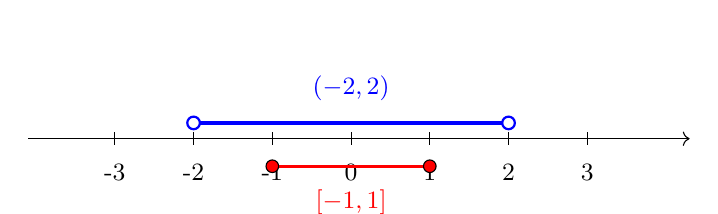
\begin{tikzpicture}[x=1cm,y=1cm]
  \draw[->] (-4.1,0) -- (4.3,0);
  \foreach \x in {-3,-2,-1,0,1,2,3}
    \draw (\x,0.08)--(\x,-0.08) node[below=0.12cm] {\small \x};
  \draw[blue,very thick] (-2,0.2)--(2,0.2);
  \draw[fill=white,draw=blue,thick] (-2,0.2) circle (0.08);
  \draw[fill=white,draw=blue,thick] (2,0.2) circle (0.08);
  \node[blue,above=0.16cm] at (0,0.2) {\small \((-2,2)\)};
  \draw[red,very thick] (-1,-0.35)--(1,-0.35);
  \draw[fill=red] (-1,-0.35) circle (0.08);
  \draw[fill=red] (1,-0.35) circle (0.08);
  \node[red,below=0.18cm] at (0,-0.35) {\small \([-1,1]\)};
\end{tikzpicture}
\caption{开区间不取端点，闭区间取端点；同一条数轴同时表示集合和距离。}
\label{fig:intervals}
\end{figure}

\begin{remark}[开集和闭集的第一眼读法]
在数轴上，一个集合 \(U\subseteq\mathbb R\) 是开集，是指它的每个点周围都能放进一个小开区间而不跑出 \(U\)：对每个 \(x\in U\)，存在 \(r>0\) 使 \((x-r,x+r)\subseteq U\)。集合 \(F\) 是闭集，是指它的补集 \(\mathbb R\setminus F\) 是开集。于是 \((a,b)\) 是开集，\([a,b]\) 是闭集；“开”与“闭”不是“有没有边界”的日常说法，而是两条精确定义。一般拓扑空间中的开集会在模块三重新正式定义。
\end{remark}

\subsection{集合符号和逻辑连接词}

\begin{definition}[集合运算与补集]\label{def:set-operations}
交集和并集分别为
\[
A\cap B=\{x:x\in A\text{ 且 }x\in B\},\qquad
A\cup B=\{x:x\in A\text{ 或 }x\in B\}.
\]
差集与补集分别为
\[
A\setminus B=\{x:x\in A\text{ 且 }x\notin B\},
\qquad
A^c:=X\setminus A\quad(A\subseteq X).
\]
所有这些运算都依赖于一个已经指定的母集合或全集；补集不是“所有不在 \(A\) 中的抽象对象”，而是“在当前全集 \(X\) 中但不在 \(A\) 中的元素”。
\end{definition}

\begin{definition}[逻辑连接词与量词]\label{def:logic-symbols}
\(P\Rightarrow Q\) 表示“若 \(P\)，则 \(Q\)”；\(P\Leftrightarrow Q\) 表示两者互相推出；\(\neg P\)、\(P\land Q\)、\(P\lor Q\) 分别表示“非 \(P\)”、“\(P\) 且 \(Q\)”和“\(P\) 或 \(Q\)”。\(\forall\) 表示“对所有”，\(\exists\) 表示“存在”，而 \(\exists!\) 表示“存在唯一”。\(:=\) 表示“定义为”，不是待证明的等式。
\end{definition}

\begin{remark}[充分、必要、逆命题与逆否命题]
命题 \(P\Rightarrow Q\) 读作“\(P\) 是 \(Q\) 的充分条件”，也读作“\(Q\) 是 \(P\) 的必要条件”。
它只规定从 \(P\) 到 \(Q\) 的方向；把方向反过来的 \(Q\Rightarrow P\) 是逆命题，通常不能自动成立。
而
\[
P\Rightarrow Q
\quad\Longleftrightarrow\quad
\neg Q\Rightarrow\neg P
\]
是逆否命题，二者逻辑等价。比如“\(n\) 能被 \(4\) 整除 \(\Rightarrow n\) 为偶数”是真的，
其逆命题“\(n\) 为偶数 \(\Rightarrow n\) 能被 \(4\) 整除”是假的；其逆否命题“\(n\) 不是偶数
\(\Rightarrow n\) 不能被 \(4\) 整除”是真的。只有同时证明 \(P\Rightarrow Q\) 和
\(Q\Rightarrow P\)，才能写 \(P\Leftrightarrow Q\)。证明中“必要”“充分”“当且仅当”
分别对应不同的方向，不能靠中文语感互换。
\end{remark}

\begin{proposition}[集合相等的证明模板]
要证明 \(A=B\)，可以证明两次包含：
\[
A\subseteq B\quad\text{且}\quad B\subseteq A.
\]
并且对任意 \(A,B\subseteq X\)，补集 \(A^c=X\setminus A\) 满足
\[
(A\cup B)^c=A^c\cap B^c,\qquad
(A\cap B)^c=A^c\cup B^c.
\]
这些等式的证明不是比较图形大小，而是任取 \(x\in X\)，逐步把“属于左边”翻译成同一个逻辑命题。
\end{proposition}

\begin{proof}
若 \(x\in(A\cup B)^c\)，则 \(x\notin A\cup B\)，所以 \(x\notin A\) 且
\(x\notin B\)，即 \(x\in A^c\cap B^c\)；反向推理相同。第二个 De Morgan 等式同理。
双重包含判据直接来自集合相等的逐元素定义。
\end{proof}

\begin{figure}[htbp]
\centering
\begin{tikzpicture}[x=1cm,y=1cm]
  \begin{scope}[xshift=-3.2cm]
    \draw[fill=blue!18,draw=blue!65!black,thick] (0,0) circle (1.0);
    \draw[fill=red!18,draw=red!65!black,thick] (1.0,0) circle (1.0);
    \node[blue!70!black] at (-0.45,0.68) {\(A\)};
    \node[red!70!black] at (1.45,0.68) {\(B\)};
    \node[figurelabel] at (0.5,-1.35) {\(A\cup B\)：至少属于一个};
  \end{scope}
  \begin{scope}[xshift=3.0cm]
    \draw[fill=blue!18,draw=blue!65!black,thick] (0,0) circle (1.0);
    \draw[fill=red!18,draw=red!65!black,thick] (1.0,0) circle (1.0);
    \node[blue!70!black] at (-0.45,0.68) {\(A\)};
    \node[red!70!black] at (1.45,0.68) {\(B\)};
    \node[figurelabel] at (0.5,-1.35) {\(A\cap B\)：同时属于两个};
  \end{scope}
\end{tikzpicture}
\caption{并集与交集的 Venn 图直觉：并集扩大“允许范围”，交集缩小到“共同范围”。}
\label{fig:set-operations-venn}
\end{figure}

\begin{example}[量词顺序为什么重要]
“对每个学生，都存在一本他喜欢的书”写作
\[
\forall x\in\text{学生},\ \exists y\in\text{书}:\ x\text{喜欢 }y.
\]
“存在一本书，所有学生都喜欢它”写作
\[
\exists y\in\text{书},\ \forall x\in\text{学生}:\ x\text{喜欢 }y.
\]
两句话的量词顺序不同，含义也不同。读极限定义时，\(\forall\varepsilon\,\exists N\) 的顺序同样不能交换。
\end{example}

\subsection{函数、图像和参数：不要把公式当成图形本身}

\Needspace{18\baselineskip}
\begin{definition}[函数]\label{def:set-function}
设 \(X,Y\) 是集合。一个从 \(X\) 到 \(Y\) 的\term{def:set-function}{映射}（或函数）是一个规则
\[
f:X\longrightarrow Y
\]
它给每个 \(x\in X\) 指定唯一的 \(f(x)\in Y\)。\(X\) 称为定义域，\(Y\) 称为陪域；
因此，一个映射的完整声明至少包含三项：输入集合 \(X\)、输出被允许落入的集合
\(Y\)，以及把每个 \(x\in X\) 送到某个 \(f(x)\in Y\) 的规则。箭头左边是定义域，
箭头右边是陪域；陪域不是“实际已经用到的输出”。
例如 \(x^2:\mathbb R\to\mathbb R\) 和
\(x^2:\mathbb R\to[0,\infty)\) 的计算规则相同，但它们是两个不同的映射，因为陪域不同。
两个映射只有在定义域和陪域都相同、且每个输入的输出都相同时，才称为同一个映射。
因此函数不是一个孤立的代数公式：改变定义域、陪域或允许的输入，可能改变它的性质。
\end{definition}

\begin{definition}[像集]\label{def:image-set}
设 \(f:X\to Y\) 是映射。\(f\) 的\term{def:image-set}{像集}定义为
\[
f(X):=\{f(x):x\in X\}\subseteq Y.
\]
它记录实际至少被一个输入命中的目标。于是总有 \(f(X)\subseteq Y\)，并且
\(f\) 满射当且仅当 \(f(X)=Y\)；改变陪域而不改变规则，可能改变这个等式是否成立。
\end{definition}

\Needspace{12\baselineskip}
\begin{definition}[原像]\label{def:preimage}
设 \(f:X\to Y\) 是映射。若 \(V\subseteq Y\)，其
\term{def:preimage}{原像}定义为
\[
  f^{-1}(V):=\{x\in X:f(x)\in V\}.
\]
它是把目标集合向输入端拉回的集合运算；这里的 \(f^{-1}(V)\) 不表示已经存在一个逆函数。
\end{definition}

\begin{definition}[纤维]\label{def:fiber}
设 \(f:X\to Y\) 是映射，\(y\in Y\)。\(y\) 在 \(f\) 下的
\term{def:fiber}{纤维}定义为
\[
  f^{-1}(\{y\})=\{x\in X:f(x)=y\}.
\]
纤维可能为空、恰有一个元素，或含有多个元素。只有当 \(f\) 是双射时，
才可以把同一个符号 \(f^{-1}\) 进一步解释为从 \(Y\) 到 \(X\) 的逆映射；此时
\[
  f^{-1}(\{y\})=\{f^{-1}(y)\}.
\]
\end{definition}

\Needspace{12\baselineskip}
\begin{definition}[函数复合]\label{def:function-composition}
若 \(f:X\to Y\)、\(g:Y\to Z\)，则可以先用 \(f\) 再用 \(g\)，得到复合映射
\[
  g\circ f:X\longrightarrow Z,
  \qquad (g\circ f)(x):=g(f(x)).
\]
这里的书写顺序从右向左读：先看 \(f\)，再看 \(g\)。只有前一个映射的陪域与后一个映射的定义域接得上，复合才有意义。
\end{definition}

\begin{definition}[恒等映射]\label{def:identity-map}
\(X\) 上的\term{def:identity-map}{恒等映射}定义为
\[
  \operatorname{id}_X:X\longrightarrow X,
  \qquad \operatorname{id}_X(x):=x.
\]
它什么也不改变；因此对任意 \(f:X\to Y\)，都有
\[
  f\circ\operatorname{id}_X=f,
  \qquad \operatorname{id}_Y\circ f=f.
\]
这些等式是后面定义逆映射、同态和群作用时的类型检查工具。
\end{definition}

\Needspace{13\baselineskip}
\begin{remark}[怎样逐字读懂箭头 \(f:X\to Y\)]\label{rem:map-arrow-reading}
读 \(f:X\to Y\) 时，可以把它翻译成一句完整的话：
“允许从 \(X\) 中拿任何一个输入；规则 \(f\) 必须给它恰好一个输出；这个输出必须属于
\(Y\)。”这句话包含三个不同的检查：
\begin{enumerate}[label=(\arabic*)]
  \item 每个输入都有输出：否则它不是定义在整个 \(X\) 上的函数；
  \item 每个输入只有一个输出：这是函数的“单值性”，不是单射性；
  \item 输出落在 \(Y\) 中：这是陪域约束，不要求 \(Y\) 中每个元素都真的出现。
\end{enumerate}
只有在这三层都成立之后，才有意义再问“是否单射”或“是否满射”。换句话说，
“单值”“单射”“满射”分别是函数存在、禁止输入碰撞、覆盖整个陪域这三个不同问题。
这里的术语对应英文 \emph{function/map}、\emph{injective (one-to-one)}、
\emph{surjective (onto)} 和 \emph{bijective}；英文括号只用于识别文献，不改变中文定义。
\end{remark}

\Needspace{18\baselineskip}
\begin{definition}[函数的集合论图像]\label{def:function-graph-formal}
设 \(X,Y\) 是集合。一个子集 \(\Gamma\subseteq X\times Y\) 恰好是某个从 \(X\) 到 \(Y\) 的函数的图像，当且仅当它满足两条条件：
\begin{enumerate}[label=(\alph*)]
  \item \textbf{全定义（存在性）：} 对每个 \(x\in X\)，至少存在一个 \(y\in Y\)，使得 \((x,y)\in\Gamma\)；
  \item \textbf{单值（唯一性）：} 对每个 \(x\in X\)，若 \((x,y_1)\in\Gamma\) 且 \((x,y_2)\in\Gamma\)，则 \(y_1=y_2\)。
\end{enumerate}
第一条说每个允许的输入都必须有输出，第二条说同一个输入不能同时被规定两个不同的输出。
两条合在一起就是
\[
  \forall x\in X\;\exists!\,y\in Y:\ (x,y)\in\Gamma,
\]
其中 \(\exists!\) 读作“存在唯一”。于是可把这个函数写成
\[
  f_\Gamma(x)=y\quad\Longleftrightarrow\quad (x,y)\in\Gamma.
\]
反过来，任意函数 \(f:X\to Y\) 都确定唯一的集合
\[
  \Gamma_f=\{(x,f(x)):x\in X\}\subseteq X\times Y.
\]
因此“函数是规则”和“函数是满足全定义、单值条件的有序对集合”是同一个对象的两种读法：前一种方便计算，后一种方便做集合论证明。
\end{definition}

\Needspace{18\baselineskip}
\begin{example}[全定义与单值分别防止什么错误]
取 \(X=\{1,2\}\)、\(Y=\{a,b,c\}\)。
\[
  \Gamma_1=\{(1,a),(2,b)\}
\]
满足全定义和单值条件，所以它表示一个函数 \(X\to Y\)；它的像集是 \(\{a,b\}\)，因而不是满射。
\[
  \Gamma_2=\{(1,a)\}
\]
不是从 \(X\) 到 \(Y\) 的函数图像，因为输入 \(2\) 没有输出；这是违反全定义。
\[
  \Gamma_3=\{(1,a),(1,b),(2,c)\}
\]
也不是函数图像，因为同一个输入 \(1\) 被送到两个不同输出；这是违反单值。
这三个例子要区分三件事：\(\Gamma_1\) 是函数但可能不满射，\(\Gamma_2\) 连函数都不是，\(\Gamma_3\) 也连函数都不是。只有先确认对象确实是函数，才有意义继续问它是否单射、满射或双射。
\end{example}

\begin{figure}[htbp]
\centering
\begin{tikzpicture}[x=1cm,y=1cm]
  % 函数图像作为 X	imes Y 中的格点集合。
  \node[font=\bfseries] at (0.85,2.12) {$\Gamma_f\subseteq X\times Y$};
  \draw[draw=black!55,fill=black!2] (-0.60,-1.50) rectangle (2.30,1.50);
  \draw[black!35] (0.37,-1.50) -- (0.37,1.50);
  \draw[black!35] (1.34,-1.50) -- (1.34,1.50);
  \draw[black!35] (-0.60,-0.50) -- (2.30,-0.50);
  \draw[black!35] (-0.60,0.50) -- (2.30,0.50);
  \node[font=\small\bfseries] at (0.85,1.78) {输入列 $x\in X$};
  \node[font=\small] at (-0.11,1.20) {$1$};
  \node[font=\small] at (0.85,1.20) {$2$};
  \node[font=\small] at (1.82,1.20) {$3$};
  \node[font=\small\bfseries,rotate=90] at (-0.98,0) {输出行 $y\in Y$};
  \node[font=\small] at (-0.37,1.00) {$a$};
  \node[font=\small] at (-0.37,0.00) {$b$};
  \node[font=\small] at (-0.37,-1.00) {$c$};
  \fill[blue!70!black] (-0.11,1.00) circle (2.6pt);
  \fill[blue!70!black] (0.85,-1.00) circle (2.6pt);
  \fill[blue!70!black] (1.82,-1.00) circle (2.6pt);
  \node[font=\scriptsize,blue!70!black] at (0.85,-1.82)
    {$\Gamma_f=\{(1,a),(2,c),(3,c)\}$};

  \node[font=\bfseries] at (5.50,2.12) {从格点读性质};
  \node[draw=blue!45!black,fill=blue!4,rounded corners=2pt,
        align=left,text width=4.70cm,inner sep=6pt,font=\small] at (5.50,0.15)
    {$\bullet$ 每列恰一点 $\Longleftrightarrow$ 函数；\\[3pt]
     $\bullet$ 每行至多一点 $\Longleftrightarrow$ 单射；\\[3pt]
     $\bullet$ 每行至少一点 $\Longleftrightarrow$ 满射；\\[3pt]
     $\bullet$ 每列、每行都恰一点 $\Longleftrightarrow$ 双射。};
\end{tikzpicture}
\caption{函数图像的格点模型。例中每一列恰有一个格点，所以它确实定义了
一个函数；第三行有两个格点，第二行没有格点，因此该函数不是单射，也不是满射。
这把函数、单射、满射、双射统一放回同一个集合 $X\times Y$ 中检查。}
\label{fig:function-graph-fiber-criteria}
\end{figure}

\Needspace{13\baselineskip}
\subsection{单射、满射与双射：无碰撞、无遗漏、逐一匹配}

这三个词只描述映射的性质，不是三种新的映射对象。必须先写出完整的
\(f:X\to Y\)，再讨论它；只写 \(f(x)=x^2\) 而不写定义域和陪域，问题通常还没有说完整。

\begin{definition}[单射、满射与双射的正式定义]
设 \(f:X\to Y\) 是一个已经给定的映射。

\begin{enumerate}[label=(\arabic*)]
  \item \label{def:injective}若
  \[
    \forall x_1,x_2\in X,\qquad
    f(x_1)=f(x_2)\Longrightarrow x_1=x_2,
  \]
  则称 \(f\) 是\term{def:injective}{单射}（injective）。它禁止两个不同输入发生碰撞。

  \item \label{def:surjective}若
  \[
    \forall y\in Y\ \exists x\in X,\qquad f(x)=y,
  \]
  则称 \(f\) 是\term{def:surjective}{满射}（surjective）。它要求陪域中的每一个目标都被命中，
  等价地要求 \(f(X)=Y\)。

  \item \label{def:bijective}若 \(f\) 同时是单射和满射，则称 \(f\) 是\term{def:bijective}{双射}（bijective）。
\end{enumerate}

这三个定义的量词方向不同：单射比较“任意两个输入”，满射从“任意目标”寻找一个输入，
双射把这两项同时要求。它们都必须相对于同一个定义域 \(X\)、同一个陪域 \(Y\) 来理解。
\end{definition}

\Needspace{18\baselineskip}
\begin{remark}[单满双的核心判定表]\label{rem:map-core-table}
这是本节唯一需要反复调用的主线。对每个目标 \(y\in Y\)，记
\[
  X_y:=f^{-1}(\{y\})=\{x\in X:f(x)=y\}.
\]
它表示“哪些输入被送到 \(y\)”。从输入端看，函数已经要求每个 \(x\) 恰有一个输出；从输出端看，才继续检查下面三种性质：
\begin{center}
\small
\begin{tabularx}{\textwidth}{p{0.16\textwidth}p{0.27\textwidth}p{0.25\textwidth}X}
\toprule
性质 & 正式要求 & 箭头图像 & 失败时寻找什么 \\
\midrule
函数（单值）
& 每个 \(x\) 是否有且只有一个 \(f(x)\)
& 每个输入只有一根箭头出去
& 一个输入没有输出，或分叉到两个输出 \\
单射
& 每个 \(X_y\) 至多有一个元素
& 不同输入不能撞到同一目标
& 找 \(x_1\ne x_2\) 但 \(f(x_1)=f(x_2)\) \\
满射
& 每个 \(X_y\) 至少有一个元素
& 陪域中的每个目标都有箭头射入
& 找 \(y\in Y\) 使 \(X_y=\varnothing\) \\
双射
& 每个 \(X_y\) 恰有一个元素
& 没有碰撞，也没有遗漏
& 只要出现碰撞或遗漏就不是双射 \\
\bottomrule
\end{tabularx}
\end{center}
因此，“单值、单射、满射”不是三个近义词：它们依次检查
“输入是否有唯一输出”“输出是否至多一个输入”“陪域目标是否至少有一个输入”。
这张表也解释了记忆句：单射消灭碰撞，满射消灭遗漏，双射同时消灭两种障碍。
\end{remark}

\Needspace{16\baselineskip}
\begin{remark}[单满双的固定四步检查台]\label{rem:map-four-step-check}
初学时不要把“单射、满射、双射”当成三个需要凭感觉记忆的形容词。
对一个完整映射 \(f:X\to Y\)，固定按下面四步走：
\begin{center}
\small
\begin{tabularx}{\textwidth}{p{0.16\textwidth}p{0.27\textwidth}p{0.22\textwidth}X}
\toprule
\text{检查顺序}&\text{正式问题}&\text{直观画面}&\text{证明或反例的动作}\\
\midrule
0.\ \text{先确认函数}
&\(\forall x\in X\ \exists!y\in Y,\ f(x)=y\)
&每个输入恰有一根箭头出去
&检查没有遗漏输入，也没有一输入分叉\\
1.\ \text{检查单射}
&\(f(x_1)=f(x_2)\Rightarrow x_1=x_2\)
&两根箭头不能撞到同一目标
&证明：任取输入对；反例：找一对碰撞\\
2.\ \text{检查满射}
&\(\forall y\in Y\ \exists x\in X,\ f(x)=y\)
&每个目标至少有一根箭头射入
&证明：任取目标解方程；反例：找一个空目标\\
3.\ \text{检查双射}
&单射且满射
&每个目标恰有一根箭头射入
&同时完成前两项，或构造双侧逆\\
\bottomrule
\end{tabularx}
\end{center}
第 \(0\) 步是“它是不是函数”，不是单射性；第 \(1\) 步从两个输入向内比较，
第 \(2\) 步从一个目标向外寻找原像。方向不同，量词也不同：
\[
\underbrace{\forall x_1,x_2}_{\text{任意两输入}}\quad\text{对比}\quad
\underbrace{\forall y\ \exists x}_{\text{任意目标找一个输入}}.
\]
这也是为什么证明单射通常从 \(f(x_1)=f(x_2)\) 开始，而证明满射通常从
“任取 \(y\in Y\)”开始。双射不是“特别快的函数”，而是同时没有碰撞、没有遗漏。
\end{remark}

\begin{example}[把四步检查完整走一遍]
令
\[
f:\{1,2,3,4\}\longrightarrow\{a,b,c\},\qquad
1\mapsto a,\quad2\mapsto b,\quad3\mapsto c,\quad4\mapsto c.
\]
第 \(0\) 步：四个输入各有且只有一个输出，所以它是函数。第 \(1\) 步：
\(f(3)=f(4)=c\)，但 \(3\ne4\)，所以它不是单射。第 \(2\) 步：
\(a,b,c\) 都被命中，所以它是满射。第 \(3\) 步：因为它不是单射，
所以它不是双射。

把它改写成纤维会更清楚：
\[
f^{-1}(\{a\})=\{1\},\qquad
f^{-1}(\{b\})=\{2\},\qquad
f^{-1}(\{c\})=\{3,4\}.
\]
三个目标的纤维都非空，所以满射；\(c\) 的纤维有两个元素，所以不单射。
这里的“纤维”不是另一种映射，而是从目标 \(y\) 回头收集所有满足 \(f(x)=y\)
的输入。后面的纤维判据会把这一读法证明成一般定理。
\end{example}

\begin{remark}[公式、图像、定义域和陪域的四层读法]
看到 \(f(x)=x^2\) 时，至少要问四个问题：规则是什么（把 \(x\) 变成 \(x^2\)），定义域是什么（允许哪些输入），陪域是什么（输出被声明放在哪个集合），以及它的集合论图像是什么（哪些有序对被收集起来）。例如
\[
  x^2:\mathbb R\to\mathbb R
  \qquad\text{和}\qquad
  x^2:\mathbb R\to[0,\infty)
\]
使用同一条计算规则和同一组有序对，但陪域不同；所以前者不是满射，后者是满射。单射性则由图像中是否出现“同一输入的不同输出”之外的另一种碰撞来判断：这里 \(1\) 与 \(-1\) 产生同一输出，因此两者都不是单射。这个层次区别正是后面讨论商映射、坐标变换和模空间映射时必须保持的类型意识。
\end{remark}

\begin{remark}[单、满、双的箭头记号与逻辑位置]\label{rem:map-arrow-notation}
在很多教材中，映射的性质会直接写进箭头：
\[
  X\mathrel{\hookrightarrow}Y
  \quad\text{表示单射},\qquad
  X\mathrel{\twoheadrightarrow}Y
  \quad\text{表示满射},\qquad
  X\xrightarrow{\ \sim\ }Y
  \quad\text{表示双射}.
\]
严格地说，这些记号都是对一个已经给定的函数 $f:X\to Y$ 的简写：
\begin{center}
\begin{tabularx}{\textwidth}{p{0.25\textwidth}p{0.31\textwidth}X}
\toprule
书写 & 完整翻译 & 它没有额外声称什么 \\
\midrule
$f:X\to Y$ & $f$ 是从 $X$ 到 $Y$ 的函数 & 不自动单射，也不自动满射 \\
$f:X\hookrightarrow Y$ & $f:X\to Y$ 且 $f$ 单射 & 不自动满射；$Y$ 可能还有未命中元素 \\
$f:X\twoheadrightarrow Y$ & $f:X\to Y$ 且 $f$ 满射 & 不自动单射；不同输入可能发生碰撞 \\
$f:X\xrightarrow{\ \sim\ }Y$ & $f:X\to Y$ 且 $f$ 双射 & 才能得到唯一的双侧逆映射 $f^{-1}:Y\to X$ \\
\bottomrule
\end{tabularx}
\end{center}
这里的“单”“满”不是说一个函数有三种不同的输出方式，而是对同一个函数提出的三种不同问题：
从输出端回看，是否至多有一个输入（单射）；是否至少有一个输入（满射）；是否恰好有一个输入（双射）。
因此必须先确认 $f$ 的定义域、陪域和函数规则，再读取箭头上的性质。特别是
\(\hookrightarrow\) 在拓扑学中有时还被作者专门约定为“拓扑嵌入”；在本段集合论语境中，
它只表示单射，拓扑嵌入的连续性和子空间条件要到后文另行加入。
\end{remark}

\begin{proposition}[单射与满射在一般集合中彼此独立]\label{prop:single-surj-independent}
在不附加有限性或等势条件时，单射性和满射性互不推出：
\[
\text{单射}\not\Longrightarrow\text{满射},\qquad
\text{满射}\not\Longrightarrow\text{单射}.
\]
例如
\[
  s:\mathbb N\to\mathbb N,\quad s(n)=n+1
\]
是单射但不是满射，因为 $0$ 没有原像；而
\[
  q:\mathbb N\to\mathbb N,\quad q(n)=\lfloor n/2\rfloor
\]
是满射但不是单射，因为 $q(0)=q(1)=0$。因此“单”和“满”是两个独立的布尔性质，
而“双射”正是它们同时成立：
\[
  \text{双射}=\text{单射}\;\land\;\text{满射}.
\]
只有在额外知道 $X,Y$ 是有限且 $|X|=|Y|$ 时，才可以用后文的有限计数定理把单射和满射互相推出。
\end{proposition}

\begin{proof}
对 $s$，若 $s(n)=s(m)$，则 $n+1=m+1$，从而 $n=m$，故 $s$ 单射；但 $s(n)\ge1$，
所以 $0$ 不在像集中，故不满射。对 $q$，任给 $k\in\mathbb N$，取 $n=2k$，则
\(q(n)=\lfloor 2k/2\rfloor=k\)，故 $q$ 满射；另一方面
\(q(0)=q(1)=0\) 且 $0\ne1$，故 $q$ 不单射。
\end{proof}

\begin{example}[同一个箭头为什么必须写全]
考虑同一条规则 $r(x)=x^2$。下面三行不是“同一个映射的三种叫法”，而是三个定义域或陪域不同的映射：
\[
  \mathbb R\xrightarrow{\ r\ }\mathbb R,
  \qquad
  \mathbb R\xrightarrow{\ r\ }[0,\infty),
  \qquad
  [0,\infty)\xrightarrow{\ r\ }[0,\infty).
\]
第一行既不单射也不满射；第二行满射但不单射；第三行是双射。变化的不是计算公式，
而是“允许哪些输入”和“把哪些目标宣告为陪域”。所以在后文看到
\(f:X\to Y\)、\(f:X\hookrightarrow Y\) 或 \(f:X\xrightarrow{\sim}Y\) 时，箭头左右的集合和箭头本身必须一起阅读。
\end{example}

\begin{proposition}[单射、满射与双射的纤维判据]\label{prop:fiber-single-surj-bijective}
设 \(f:X\to Y\) 是映射。对每个 \(y\in Y\)，记纤维
\[
  X_y:=f^{-1}(\{y\})=\{x\in X:f(x)=y\}.
\]
则
\[
\begin{array}{rcl}
 f\text{ 是单射} &\Longleftrightarrow& X_y\text{ 至多含有一个元素}\quad(\forall y\in Y),\\[0.25em]
 f\text{ 是满射} &\Longleftrightarrow& X_y\text{ 至少含有一个元素}\quad(\forall y\in Y),\\[0.25em]
 f\text{ 是双射} &\Longleftrightarrow& X_y\text{ 恰好含有一个元素}\quad(\forall y\in Y).
\end{array}
\]
这里暂时不用集合基数记号，只数“没有、一个、还是多个”；后文正式定义基数后，
这三行也可简写为 \(|X_y|\le1\)、\(|X_y|\ge1\) 和 \(|X_y|=1\)。
空纤维正是陪域中没有被命中的点。
\end{proposition}

\begin{proof}
若 \(f\) 单射，某个纤维中若有 \(x_1,x_2\)，则
\(f(x_1)=f(x_2)=y\)，从而 \(x_1=x_2\)，故每个纤维至多一个元素。反过来，若每个纤维至多一个元素，
由 \(f(x_1)=f(x_2)=y\) 可知 \(x_1,x_2\in X_y\)，所以 \(x_1=x_2\)。
满射的定义正是每个 \(y\in Y\) 至少有一个原像，即每个纤维非空。双射同时满足前两项，
于是每个纤维恰含一个元素；反向也同理。
\end{proof}

\begin{remark}[单满双的统一读法]\label{rem:single-surj-bijective-read}
纤维语言把三种性质压缩成一条数量链：空纤维对应陪域遗漏，含有两个不同元素的纤维对应输入碰撞；因此单射要求“没有多于一个”，满射要求“没有空的”，双射要求“每个恰好一个”。正式的等价证明见\term{prop:fiber-single-surj-bijective}{纤维的单满双判据}。若集合还带有拓扑、光滑或复结构，单满双只描述底层集合，还必须另行检查连续、光滑或全纯等条件。
\end{remark}

\begin{definition}[逆映射]\label{def:inverse-map}
设 \(f:X\to Y\) 是双射。对每个 \(y\in Y\)，由于满射性至少存在一个
\(x\in X\) 使 \(f(x)=y\)，由于单射性这样的 \(x\) 至多有一个；因此可以定义
\term{def:inverse-map}{逆映射}
\[
  f^{-1}:Y\longrightarrow X,
  \qquad f^{-1}(y):=\text{满足 }f(x)=y\text{ 的唯一 }x.
\]
这里的 \(f^{-1}\) 是一个新的映射，定义域与陪域都与 \(f\) 交换；它不是原像运算
\(V\mapsto f^{-1}(V)\) 的缩写。由定义，
\[
  f^{-1}\circ f=\operatorname{id}_X,
  \qquad f\circ f^{-1}=\operatorname{id}_Y.
\]
\end{definition}

\begin{remark}[函数、单射、满射与双射的四层量词链]\label{rem:map-quantifier-chain}
量词的方向是最可靠的记忆工具：函数是“\(\forall x\in X\,\exists!y\in Y\)”；单射是“任意两个输入若输出相同，则输入相同”；满射是“\(\forall y\in Y\,\exists x\in X\)”；双射是后两者同时成立。单值性发生在输入端，单射性和满射性发生在输出端，不能把三个“每个”混读。
\end{remark}

\begin{proposition}[像集、纤维与陪域缺口的对应]\label{prop:image-fiber-criterion}
设 \(f:X\to Y\) 是映射，并对 \(y\in Y\) 记纤维为
\(X_y=f^{-1}(\{y\})\)。则
\[
  f(X)=\{y\in Y:X_y\ne\varnothing\},
  \qquad
  Y\setminus f(X)=\{y\in Y:X_y=\varnothing\}.
\]
更一般地，对任意 \(V\subseteq Y\)，
\[
  f^{-1}(V)=\bigcup_{y\in V}X_y.
\]
因此：满射性是在问“有没有空纤维”；单射性是在问“有没有含两个不同元素的纤维”；
双射性是在问“每个纤维是否恰好含一个元素”。
\end{proposition}

\begin{proof}
对任意 \(y\in Y\)，有
\[
 y\in f(X)
 \Longleftrightarrow \exists x\in X,\ f(x)=y
 \Longleftrightarrow X_y\ne\varnothing.
\]
对两边取 \(Y\) 中的补集，得到第二个等式。再对任意 \(x\in X\) 计算：
\[
 x\in f^{-1}(V)
 \Longleftrightarrow f(x)\in V
 \Longleftrightarrow x\in X_{f(x)}\text{ 且 }f(x)\in V
 \Longleftrightarrow x\in\bigcup_{y\in V}X_y.
\]
这说明原像集合确实是把 \(V\) 中每个目标的纤维全部收集起来。
\end{proof}

\begin{proposition}[单满双的集合运算判据]\label{prop:map-set-theoretic-criterion}
设 \(f:X\to Y\) 是映射。对任意 \(A\subseteq X\) 和 \(B\subseteq Y\)，总有
\[
A\subseteq f^{-1}(f(A)),\qquad f(f^{-1}(B))\subseteq B.
\]
其中两条包含关系的差异分别来自“可能发生碰撞”和“可能存在遗漏”。更精确地，
\[
\begin{array}{rcl}
f\text{ 单射}
&\Longleftrightarrow&
f^{-1}(f(A))=A\quad(\forall A\subseteq X),\\[0.35em]
f\text{ 满射}
&\Longleftrightarrow&
f(f^{-1}(B))=B\quad(\forall B\subseteq Y),\\[0.35em]
f\text{ 双射}
&\Longleftrightarrow&
\text{上面两类等式都对所有子集成立}.
\end{array}
\]
因此，单射可以理解为“先取像再取原像不会把不同输入混在一起”，满射可以理解为
“先取原像再取像不会让陪域中的目标凭空消失”。
\end{proposition}

\begin{proof}
若 \(x\in A\)，则 \(f(x)\in f(A)\)，所以 \(x\in f^{-1}(f(A))\)，得到第一条包含关系。
若 \(y\in f(f^{-1}(B))\)，则存在 \(x\in X\)，使 \(x\in f^{-1}(B)\) 且 \(f(x)=y\)；
由原像定义 \(f(x)\in B\)，故 \(y\in B\)，得到第二条包含关系。

若 \(f\) 单射，取 \(x\in f^{-1}(f(A))\)，则存在 \(a\in A\) 使
\(f(x)=f(a)\)；单射性给出 \(x=a\)，故 \(x\in A\)，于是第一条包含关系成为等式。
反之，若对所有 \(A\) 都有 \(f^{-1}(f(A))=A\)，取
\(A=\{x_1\}\)。若 \(f(x_1)=f(x_2)\)，则
\(x_2\in f^{-1}(f(\{x_1\}))=\{x_1\}\)，所以 \(x_2=x_1\)，故 \(f\) 单射。

若 \(f\) 满射，取 \(y\in B\)。存在 \(x\in X\) 使 \(f(x)=y\)，于是
\(x\in f^{-1}(B)\)，从而 \(y\in f(f^{-1}(B))\)；结合第二条包含关系得到等式。
反之，若对所有 \(B\) 都有 \(f(f^{-1}(B))=B\)，取 \(B=\{y\}\)。等式说明
\(y\in f(f^{-1}(\{y\}))\)，故存在 \(x\in X\) 使 \(f(x)=y\)，于是 \(f\) 满射。
双射的结论就是把单射和满射两项合并。
\end{proof}

\begin{remark}[为什么保留两个不同的判据]
前面的\term{prop:fiber-single-surj-bijective}{纤维的单满双判据}回答的是“单射、满射、
双射分别等价于什么”；本命题回答的是“像集和原像集合由哪些纤维组成”。二者不重复：
前者是检验映射类型的三条门槛，后者是计算像集、原像和陪域中遗漏部分的集合公式。
在后面的商映射、投影和解析族中，常常先算纤维，再用这两个不同层次的结论判断性质。
\end{remark}

\Needspace{15\baselineskip}
\begin{remark}[“单值”与“单射”不是同一件事]
“单值”是\term{def:function-graph-formal}{函数图像}的基本要求：一个输入只能有一个输出，
否则它甚至还不是函数。例如
\[
  \{(1,a),(2,a)\}\quad\text{是函数图像，}
  \qquad
  \{(1,a),(1,b)\}\quad\text{不是函数图像（若 }a\ne b\text{）。}
\]
但前一个函数不是单射，因为两个不同输入 \(1,2\) 碰撞到了同一个输出 \(a\)。
因此要按两个不同层次阅读：
\[
\begin{array}{c|c|c}
\text{问题}&\text{检查方向}&\text{失败时的现象}\\
\hline
\text{它是不是函数？}&\text{一个输入向外看}&\text{一个输入没有输出，或有两个输出}\\
\text{它是不是单射？}&\text{两个输入向内比较}&\text{两个不同输入得到同一输出}\\
\text{它是不是满射？}&\text{一个陪域元素向内寻找}&\text{某个目标没有任何原像}
\end{array}
\]
在实平面图像中，第一问对应“竖直线不能穿过两个点”（竖线检验）；第二问对应“水平线不能穿过两个点”（水平线检验）。
水平线检验只适用于已经给定为实函数图像的情形，不能取代一般集合上的量词定义。
\end{remark}

\Needspace{11\baselineskip}
\begin{remark}[三种性质的否定：证明和反例各需要什么]
把定义中的量词完整地翻转，可以得到三种性质的否定：
\[
\begin{array}{rcl}
f\text{ 不是单射}
&\Longleftrightarrow&
\exists x_1,x_2\in X,\quad x_1\ne x_2\ \text{且}\ f(x_1)=f(x_2),\\[0.35em]
f\text{ 不是满射}
&\Longleftrightarrow&
\exists y\in Y,\quad\forall x\in X,\ f(x)\ne y,\\[0.35em]
f\text{ 不是双射}
&\Longleftrightarrow&
(f\text{ 不是单射})\ \text{或}\ (f\text{ 不是满射}).
\end{array}
\]
所以证明单射时，必须从“任意一对输入发生同一输出”推出输入相等；证明满射时，
必须从“任意目标输出”反解出一个合法输入。反例的工作量恰好相反：单射只需找到
一对碰撞输入，满射只需找到一个没有原像的陪域元素。这里的“任意”和“存在一个”
是逻辑上的不同，不是写作风格上的不同。
\end{remark}

\begin{example}[三种性质的最小模型]
令 \(X=\{1,2,3\}\)、\(Y=\{a,b,c,d\}\)。
\[
\begin{array}{c|c|c}
\text{映射（含定义域/陪域）}&\text{像集}&\text{性质}\\
\hline
f_1:\{1,2,3\}\to\{a,b,c,d\},\quad
1\mapsto a,\ 2\mapsto b,\ 3\mapsto c&\{a,b,c\}&\text{单射但不满射}\\
f_2:\{1,2,3\}\to\{a,b,c,d\},\quad
1\mapsto a,\ 2\mapsto a,\ 3\mapsto b&\{a,b\}&\text{既不单射也不满射}\\
f_3:\{1,2,3,4\}\to\{a,b,c\},\quad
1\mapsto a,\ 2\mapsto b,\ 3\mapsto c,\ 4\mapsto c&\{a,b,c\}&\text{满射但不单射}
\end{array}
\]
最后一行使用的定义域是 \(\{1,2,3,4\}\)，而陪域是 \(\{a,b,c\}\)，故它展示的是
“有碰撞但没有遗漏”；若把同一条规则的陪域改成 \(\{a,b,c,d\}\)，它立刻不再满射。
这个例子说明：判断满射时，不能只看公式和像的“形状”，必须把声明中的陪域写在眼前。
\end{example}

\Needspace{10\baselineskip}
\begin{example}[同一条公式怎样产生不同的映射类型]
下面每一行都是不同的映射，因为定义域或陪域的声明不同：
\[
\begin{array}{c|c|c|c}
\text{映射}&\text{单射}&\text{满射}&\text{理由}\\
\hline
x^2:\mathbb R\to\mathbb R&\text{否}&\text{否}&1,-1\text{ 碰撞；负数没有原像}\\
x^2:\mathbb R\to[0,\infty)&\text{否}&\text{是}&y\ge0\text{ 时可取 }x=\sqrt y\text{; 仍有碰撞}\\
x^2:[0,\infty)\to[0,\infty)&\text{是}&\text{是}&y\ge0\text{ 时唯一取 }x=\sqrt y\\
\sin:\mathbb R\to[-1,1]&\text{否}&\text{是}&\sin 0=\sin(2\pi)\text{; 每个 }y\in[-1,1]\text{ 有原像}
\end{array}
\]
第三行是双射，逆映射为 \(y\mapsto\sqrt y\)。第四行虽然满射，却不是单射；“周期性”给出了无穷多组碰撞。
这个表格体现一个重要原则：\emph{公式本身不携带完整的映射类型；映射类型属于“公式加定义域、陪域”的整体。}
\end{example}

\begin{definition}[有限集合]\label{def:finite-set}
集合 \(X\) 称为\term{def:finite-set}{有限集合}，是指存在某个 \(n\in\mathbb N\)，使 \(X\) 与
\(\{0,1,\ldots,n-1\}\) 之间存在双射。这里先定义“有限”这一性质；用来表示元素个数的基数记号在下一条定义中固定。
\end{definition}

\begin{definition}[基数]\label{def:cardinality}
若有限集合 \(X\) 与 \(\{0,1,\ldots,n-1\}\) 之间存在双射，则这个唯一的 \(n\) 记为
\(|X|=n\)，称为 \(X\) 的\term{def:cardinality}{基数}。空集的基数是 \(|\varnothing|=0\)。
两个有限集合满足 \(|X|=|Y|\)，当且仅当它们之间存在双射；这把“数目相同”转成了一个关于映射性质的正式结论。
\end{definition}

\begin{proposition}[有限集合的基数障碍]
设 \(X,Y\) 是有限集合，\(f:X\to Y\)。
\begin{enumerate}[label=(\alph*)]
  \item 若 \(f\) 是单射，则 \(|X|\le |Y|\)；
  \item 若 \(f\) 是满射，则 \(|Y|\le |X|\)；
  \item 因而若 \(|X|>|Y|\)，不存在从 \(X\) 到 \(Y\) 的单射；若 \(|X|<|Y|\)，不存在从 \(X\) 到 \(Y\) 的满射。
\end{enumerate}
这里的“障碍”不是凭直觉数箭头，而是把单射的“无碰撞”或满射的“无遗漏”与有限计数结合起来的正式结论。
\end{proposition}

\begin{proof}
单射把 \(X\) 中的不同元素送到 \(Y\) 中的不同元素，故像集有 \(|X|\) 个元素，而像集包含于 \(Y\)，得到 \(|X|\le |Y|\)。
满射意味着 \(Y=f(X)\)，每个目标都至少由一个输入覆盖，因此目标元素的数量不超过输入元素数量，得到 \(|Y|\le |X|\)。第三条是前两条的逆否命题。
\end{proof}

\Needspace{13\baselineskip}
\begin{remark}[单满双的检查顺序与反例模板]
面对一个具体函数，三个性质对应三种不同的检查动作：
\begin{center}
\begin{tabularx}{\textwidth}{p{0.17\textwidth}p{0.38\textwidth}X}
\toprule
性质 & 证明时要做什么 & 否定它只需找到什么 \\
\midrule
单射 & 任取 \(x_1,x_2\in X\)，从 \(f(x_1)=f(x_2)\) 推出 \(x_1=x_2\) & 一对不同输入 \(x_1\ne x_2\) 却有同一输出 \\
满射 & 任取 \(y\in Y\)，解方程 \(f(x)=y\)，并证明解 \(x\) 在 \(X\) 中 & 一个陪域元素 \(y\in Y\) 根本没有原像 \\
双射 & 同时完成前两项，或直接写出双向逆映射 & 碰撞或遗漏任意一种即可 \\
\bottomrule
\end{tabularx}
\end{center}
这里“任取”与“找一个”不能交换：证明单射和满射时分别面对任意的输入对、任意的目标输出；构造反例时只需提供一个具体见证。特别要再次强调，满射永远是相对于陪域 \(Y\) 而不是相对于公式本身讨论的。
\end{remark}

\Needspace{8\baselineskip}
\begin{remark}[空集边界不能省略]
若 \(X=\varnothing\)，从 \(X\) 到任意 \(Y\) 的映射只有一个，而且它自动是单射；
它只有在 \(Y=\varnothing\) 时才是满射。若 \(Y=\varnothing\)，只有当 \(X=\varnothing\)
时才存在映射 \(X\to Y\)。因此许多“投影”“常值映射”的简洁结论都会额外假设
相关集合非空；这不是技术性装饰，而是量词在空集上的真实行为。
\end{remark}

\begin{proposition}[每个映射都分解为“到像集的满射”再“包含进陪域”]
\label{prop:map-image-factorization}
设 \(f:X\to Y\)，令 \(I=f(X)\)。定义
\[
\widetilde f:X\longrightarrow I,\qquad \widetilde f(x)=f(x),
\qquad
\iota:I\hookrightarrow Y,\qquad \iota(u)=u.
\]
则
\[
f=\iota\circ\widetilde f,
\]
\(\widetilde f\) 总是满射，\(\iota\) 总是单射。此外，
\[
\begin{array}{c|c}
\text{\(f\) 的性质}&\text{等价描述}\\
\hline
\text{单射}&\widetilde f\text{ 是双射}\\
\text{满射}&I=Y\text{，也就是 }\iota\text{ 也是满射}\\
\text{双射}&\widetilde f\text{ 与 }\iota\text{ 都是双射}
\end{array}
\]
这不是把一个映射换成另一个映射，而是把“实际覆盖了哪些目标”和“陪域还允许哪些目标”
分开记录。
\end{proposition}

\begin{proof}
由 \(I=f(X)\) 的定义，\(\widetilde f(x)\) 的值确实属于 \(I\)，且每个 \(u\in I\)
都有某个 \(x\in X\) 使 \(\widetilde f(x)=u\)，所以 \(\widetilde f\) 满射。
\(\iota\) 是子集包含映射，因而单射。对任意 \(x\in X\)，
\((\iota\circ\widetilde f)(x)=\iota(f(x))=f(x)\)，故分解成立。
\(\widetilde f\) 单射正是 \(f\) 单射；它已知满射，所以前者双射当且仅当 \(f\) 单射。
最后，\(\iota\) 满射当且仅当 \(I=Y\)，而这正是 \(f\) 满射的定义。
\end{proof}

\begin{example}[“碰撞”和“遗漏”在分解中分别在哪里]
考虑
\[
f:\mathbb R\longrightarrow\mathbb R,\qquad f(x)=x^2.
\]
它的像集是 \(I=[0,\infty)\)，所以分解为
\[
\mathbb R\xrightarrow{\ \widetilde f\ }[0,\infty)
\lhook\joinrel\xrightarrow{\ \iota\ }\mathbb R.
\]
第一步 \(\widetilde f\) 是满射但不是单射：\(1\) 和 \(-1\) 发生碰撞；
第二步 \(\iota\) 是单射但不是满射：负数被陪域允许，却没有被命中。
于是原映射同时出现“碰撞”和“遗漏”。这个例子把单射问题放在第一步、满射问题放在
第二步，正是判定单满双时最有用的结构图。
\end{example}

\begin{proposition}[有限集合中的三者等价]\label{prop:finite-single-surj}
设 \(X,Y\) 是有限集合，且 \(|X|=|Y|\)。对任意映射 \(f:X\to Y\)，下列条件等价：
\[
f\text{ 单射}\quad\Longleftrightarrow\quad
f\text{ 满射}\quad\Longleftrightarrow\quad
f\text{ 双射}.
\]
这里的前提 \(|X|=|Y|\) 不可省略；它是有限计数原理的结果，不适用于一般无限集合。
例如 \(\mathbb N\to\mathbb N,\ n\mapsto n+1\) 是单射却不是满射，因为 \(0\) 没有原像；
\(\mathbb N\to\mathbb N,\ n\mapsto\lfloor n/2\rfloor\) 是满射却不是单射。
\end{proposition}

\begin{proof}
有限集合中，若单射，则不同输入产生 \(|X|\) 个不同输出；由于 \(Y\) 只有同样多的
\(|Y|=|X|\) 个元素，这些输出必然正好用完 \(Y\)，故满射。若满射，则 \(Y\) 的每个
元素都有原像；若有两个不同输入落到同一输出，就会使不同输入的数量超过可用目标的
数量，故必须单射。双射按定义等价于两者同时成立。
\end{proof}

\begin{figure}[htbp]
\centering
\begin{tikzpicture}[x=1cm,y=0.72cm]
  \begin{scope}[xshift=-4.8cm]
    \node[figurelabel] at (0,3.4) {单射但不满射};
    \node[circle,draw,inner sep=1.2pt] (ixone) at (-0.55,2.5) {\scriptsize \(x_1\)};
    \node[circle,draw,inner sep=1.2pt] (ixtwo) at (-0.55,1.55) {\scriptsize \(x_2\)};
    \node[circle,draw,inner sep=1.2pt] (ixthree) at (-0.55,0.6) {\scriptsize \(x_3\)};
    \node[circle,draw,inner sep=1.2pt] (iyone) at (0.55,2.5) {\scriptsize \(y_1\)};
    \node[circle,draw,inner sep=1.2pt] (iytwo) at (0.55,1.55) {\scriptsize \(y_2\)};
    \node[circle,draw,inner sep=1.2pt] (iythree) at (0.55,0.6) {\scriptsize \(y_3\)};
    \node[circle,draw,inner sep=1.2pt] (iyfour) at (0.55,-0.35) {\scriptsize \(y_4\)};
    \draw[diagramarrow] (ixone)--(iytwo);
    \draw[diagramarrow] (ixtwo)--(iyone);
    \draw[diagramarrow] (ixthree)--(iyfour);
    \node[figurelabel] at (0,-0.95) {无碰撞；\(y_3\) 未被命中};
  \end{scope}
  \begin{scope}
    \node[figurelabel] at (0,3.4) {满射但不单射};
    \node[circle,draw,inner sep=1.2pt] (sxone) at (-0.55,2.5) {\scriptsize \(x_1\)};
    \node[circle,draw,inner sep=1.2pt] (sxtwo) at (-0.55,1.55) {\scriptsize \(x_2\)};
    \node[circle,draw,inner sep=1.2pt] (sxthree) at (-0.55,0.6) {\scriptsize \(x_3\)};
    \node[circle,draw,inner sep=1.2pt] (sxfour) at (-0.55,-0.35) {\scriptsize \(x_4\)};
    \node[circle,draw,inner sep=1.2pt] (syone) at (0.55,2.0) {\scriptsize \(y_1\)};
    \node[circle,draw,inner sep=1.2pt] (sytwo) at (0.55,0.75) {\scriptsize \(y_2\)};
    \node[circle,draw,inner sep=1.2pt] (sythree) at (0.55,-0.35) {\scriptsize \(y_3\)};
    \draw[diagramarrow] (sxone)--(syone);
    \draw[diagramarrow] (sxtwo)--(syone);
    \draw[diagramarrow] (sxthree)--(sytwo);
    \draw[diagramarrow] (sxfour)--(sythree);
    \node[figurelabel] at (0,-0.95) {无遗漏；\(x_1,x_2\) 发生碰撞};
  \end{scope}
  \begin{scope}[xshift=4.8cm]
    \node[figurelabel] at (0,3.4) {双射};
    \node[circle,draw,inner sep=1.2pt] (bxone) at (-0.55,2.5) {\scriptsize \(x_1\)};
    \node[circle,draw,inner sep=1.2pt] (bxtwo) at (-0.55,1.55) {\scriptsize \(x_2\)};
    \node[circle,draw,inner sep=1.2pt] (bxthree) at (-0.55,0.6) {\scriptsize \(x_3\)};
    \node[circle,draw,inner sep=1.2pt] (byone) at (0.55,2.5) {\scriptsize \(y_1\)};
    \node[circle,draw,inner sep=1.2pt] (bytwo) at (0.55,1.55) {\scriptsize \(y_2\)};
    \node[circle,draw,inner sep=1.2pt] (bythree) at (0.55,0.6) {\scriptsize \(y_3\)};
    \draw[diagramarrow] (bxone)--(bytwo);
    \draw[diagramarrow] (bxtwo)--(bythree);
    \draw[diagramarrow] (bxthree)--(byone);
    \node[figurelabel] at (0,-0.95) {无碰撞，也无遗漏};
  \end{scope}
\end{tikzpicture}
\caption{单射、满射与双射的具体箭头图：先看是否碰撞，再看陪域是否有遗漏。}
\label{fig:function-types}
\end{figure}

\begin{proposition}[双射恰好具有逆映射]\label{prop:bijective-inverse}
映射 \(f:X\to Y\) 是双射，当且仅当存在唯一映射 \(f^{-1}:Y\to X\)，满足
\[
f^{-1}\circ f=\operatorname{id}_X,\qquad
f\circ f^{-1}=\operatorname{id}_Y.
\]
\end{proposition}

\begin{proof}
若 \(f\) 是双射，则对每个 \(y\in Y\)，存在唯一 \(x\in X\) 使 \(f(x)=y\)；
定义 \(f^{-1}(y)=x\)，两条复合等式立即成立。反之，若这样的 \(f^{-1}\) 存在，
则 \(f(x_1)=f(x_2)\) 时对两边作用 \(f^{-1}\) 得 \(x_1=x_2\)，所以 \(f\) 单射；
对任意 \(y\in Y\)，取 \(x=f^{-1}(y)\)，则 \(f(x)=y\)，所以 \(f\) 满射。
最后说明唯一性：若 \(k:Y\to X\) 也满足
\(k\circ f=\operatorname{id}_X\) 和 \(f\circ k=\operatorname{id}_Y\)，则对任意 \(y\in Y\)，
\[
  k(y)=k\bigl(f(f^{-1}(y))\bigr)
      =(k\circ f)(f^{-1}(y))=f^{-1}(y).
\]
故 \(k=f^{-1}\)。
\end{proof}

\Needspace{12\baselineskip}
\begin{remark}[三种情形下“逆”的含义不同]\label{rem:inverse-three-cases}
“求逆”容易把三个不同问题混在一起。若 \(f\) 是单射但不满射，\(f^{-1}\) 可以作为
\[
f(X)\longrightarrow X
\]
的函数，但通常不能写成 \(Y\to X\)，因为 \(Y\setminus f(X)\) 中的目标没有原像。
若 \(f\) 是满射但不单射，每个 \(y\in Y\) 至少有一个原像，但某些 \(y\) 有多个原像，
所以不存在由 \(y\) 唯一决定的逆函数；只有在额外给出“为每个 \(y\) 选择一个原像”的规则
时，才能得到一个右逆，而这个选择一般不是唯一的，也不是双射意义下的逆。若 \(f\) 既不单射
也不满射，这两种障碍同时存在。
因此，符号 \(f^{-1}(\{y\})\) 总是可以表示纤维，而把 \(f^{-1}(y)\) 当作一个确定的
逆函数值，则必须先证明 \(f\) 双射。
\end{remark}

\begin{proposition}[复合映射对单满双性质的传递]\label{prop:composition-function-types}
设 \(f:X\to Y\)、\(g:Y\to Z\)。则：
\begin{enumerate}[label=(\alph*)]
  \item 若 \(f\) 和 \(g\) 都是单射，则 \(g\circ f\) 是单射；
  \item 若 \(f\) 和 \(g\) 都是满射，则 \(g\circ f\) 是满射；
  \item 若 \(g\circ f\) 是单射，则 \(f\) 是单射；
  \item 若 \(g\circ f\) 是满射，则 \(g\) 是满射；
  \item 若 \(f\) 和 \(g\) 都是双射，则 \(g\circ f\) 是双射，且
  \[
    (g\circ f)^{-1}=f^{-1}\circ g^{-1}.
  \]
\end{enumerate}
其余把单射性或满射性反向推回 \(g\) 或 \(f\) 的方向一般不成立：复合可能掩盖中间映射的遗漏或碰撞。
\end{proposition}

\begin{proof}
若 \(g(f(x_1))=g(f(x_2))\)，先由 \(g\) 单射得 \(f(x_1)=f(x_2)\)，再由 \(f\) 单射得
\(x_1=x_2\)，证明 (a)。若 \(z\in Z\)，由 \(g\) 满射取 \(y\in Y\) 使 \(g(y)=z\)，
再由 \(f\) 满射取 \(x\in X\) 使 \(f(x)=y\)，故 \(g(f(x))=z\)，证明 (b)。
若 \(f(x_1)=f(x_2)\)，则复合的单射性给出 \(x_1=x_2\)，证明 (c)。若 \(z\in Z\)，
复合满射性给出某个 \(x\in X\) 使 \(g(f(x))=z\)，令 \(y=f(x)\)，便有 \(g(y)=z\)，
证明 (d)。若 \(f,g\) 都是双射，则 (a)、(b) 同时成立，所以复合是双射；直接计算
\[
  (f^{-1}\circ g^{-1})\circ(g\circ f)=\operatorname{id}_X,
  \qquad
  (g\circ f)\circ(f^{-1}\circ g^{-1})=\operatorname{id}_Z,
\]
故由双射逆映射判据得到所写的逆公式。
\end{proof}

\begin{proposition}[复合的精确像、单射与满射判据]
\label{prop:composition-image-criterion}
设 \(f:X\to Y\)、\(g:Y\to Z\)。则
\[
  (g\circ f)(X)=g(f(X)),
\]
并且
\begin{align*}
  g\circ f\text{ 满射}
  &\Longleftrightarrow g(f(X))=Z,\\
  g\circ f\text{ 单射}
  &\Longleftrightarrow
  \left\{
  \begin{array}{l}
  f\text{ 单射，且}\vspace{0.2em}\\
  u_1,u_2\in f(X),\ g(u_1)=g(u_2)\Rightarrow u_1=u_2.
  \end{array}\right.
\end{align*}
因此，\(g\circ f\) 满射只要求 \(g\) 覆盖 \(Z\) 所需的那一部分中间值；
\(g\) 在 \(Y\setminus f(X)\) 上如何取值并不影响复合的满射性。类似地，
判断复合的单射性时，只需检查 \(g\) 在实际中间像集 \(f(X)\) 上是否制造碰撞。
\end{proposition}

\begin{proof}
对像集，按定义有
\[
  z\in(g\circ f)(X)
  \Longleftrightarrow \exists x\in X,\ z=g(f(x))
  \Longleftrightarrow z\in g(f(X)).
\]
第一条等价式随即由满射的定义得到。若 \(g\circ f\) 单射，先令
\(f(x_1)=f(x_2)\)，便得到 \(g(f(x_1))=g(f(x_2))\)，从而 \(x_1=x_2\)，故 \(f\) 单射；
若 \(u_i=f(x_i)\in f(X)\) 且 \(g(u_1)=g(u_2)\)，则复合的单射性给出
\(x_1=x_2\)，所以 \(u_1=u_2\)。反过来，若这两项成立且
\(g(f(x_1))=g(f(x_2))\)，先由第二项得 \(f(x_1)=f(x_2)\)，再由 \(f\) 单射得
\(x_1=x_2\)。
\end{proof}

\begin{example}[为什么其余方向不能补上]
“\(f\) 单射所以 \(g\circ f\) 单射”是错的：取
\(X=\{1,2\}\)、\(Y=\{a,b\}\)，令 \(f(1)=a,f(2)=b\)，再令
\(g(a)=g(b)=0\)，则 \(f\) 单射而 \(g\circ f\) 把两个输入都送到 \(0\)。
同样，“\(g\) 满射所以 \(g\circ f\) 满射”也不对：取
\(Y=\{a,b\}\)、\(Z=\{0,1\}\)，令 \(g(a)=0,g(b)=1\)，但令
\(f:X\to Y\) 的像只包含 \(a\)，则复合只命中 \(0\)。
这两个反例分别说明：单射性可能被后一个映射制造的碰撞破坏，满射性可能因为前一个映射没有把中间点全部送到而失效。
\end{example}

\Needspace{14\baselineskip}
\begin{definition}[左逆]\label{def:left-inverse}
设 \(f:X\to Y\) 是映射。若存在映射 \(r:Y\to X\)，使
\[
 r\circ f=\operatorname{id}_X,
\]
则称 \(r\) 是 \(f\) 的\term{def:left-inverse}{左逆}；它表示先用 \(f\) 送出，再用 \(r\) 可以恢复原输入。
\end{definition}

\begin{definition}[右逆]\label{def:right-inverse}
设 \(f:X\to Y\) 是映射。若存在映射 \(s:Y\to X\)，使
\[
 f\circ s=\operatorname{id}_Y,
\]
则称 \(s\) 是 \(f\) 的\term{def:right-inverse}{右逆}；它表示陪域中的每个目标都能由 \(s\) 选出一个原像。
\end{definition}

\begin{remark}[左逆与右逆的命名]
左逆和右逆的名称取决于它们出现在复合式的哪一侧，不是说它们本身一定是双射。
\end{remark}

\begin{proposition}[单射与满射的单侧逆判据]\label{prop:one-sided-inverse}
若 \(f:X\to Y\) 有左逆，则 \(f\) 是单射；若 \(f\) 有右逆，则 \(f\) 是满射。
若 \(f\) 是双射，则其左逆和右逆都等于唯一的逆映射 \(f^{-1}\)。
\end{proposition}

\begin{proof}
若 \(r\circ f=\operatorname{id}_X\)，且 \(f(x_1)=f(x_2)\)，则
\[
x_1=r(f(x_1))=r(f(x_2))=x_2,
\]
所以 \(f\) 单射。若 \(f\circ s=\operatorname{id}_Y\)，对任意 \(y\in Y\) 有
\(y=f(s(y))\)，所以 \(f\) 满射。最后，若 \(f\) 双射，前面的逆映射命题给出唯一
\(f^{-1}\)，任何左逆或右逆都必须与它相同。
\end{proof}

\begin{proposition}[单射与满射的消去判据]\label{prop:cancellation-injective-surjective}
设 \(f:X\to Y\) 是映射。下列两个充要条件分别成立：
\begin{align*}
 f\text{ 单射}
 &\Longleftrightarrow
 \Bigl[\text{对任意集合 }Z\text{ 及任意 }u,v:Z\to X,\quad
 f\circ u=f\circ v\Longrightarrow u=v\Bigr],\\
 f\text{ 满射}
 &\Longleftrightarrow
 \Bigl[\text{对任意集合 }Z\text{ 及任意 }u,v:Y\to Z,\quad
 u\circ f=v\circ f\Longrightarrow u=v\Bigr].
\end{align*}
第一条说：若 \(f\) 单射，把两个映射先送进 \(f\) 后仍然相同，则它们原来就相同；
第二条说：若 \(f\) 满射，两个定义在 \(Y\) 上的映射只要在 \(f\) 的像上相同，就必然在整个
\(Y\) 上相同。它们是单满双判据在“比较映射”层面的版本。
\end{proposition}

\begin{proof}
若 \(f\) 单射，且 \(f\circ u=f\circ v\)，则对每个 \(z\in Z\)，
\[
 f(u(z))=(f\circ u)(z)=(f\circ v)(z)=f(v(z)),
\]
由单射性得到 \(u(z)=v(z)\)，故 \(u=v\)。反之，若对所有 \(Z,u,v\) 都有该消去性质，
取 \(Z=\{\ast\}\)，令 \(u(\ast)=x_1\)、\(v(\ast)=x_2\)。当 \(f(x_1)=f(x_2)\) 时，
有 \(f\circ u=f\circ v\)，于是 \(u=v\)，从而 \(x_1=x_2\)，故 \(f\) 单射。

若 \(f\) 满射，且 \(u\circ f=v\circ f\)，任取 \(y\in Y\)，由满射性取 \(x\in X\) 使
\(f(x)=y\)，则
\[
u(y)=u(f(x))=(u\circ f)(x)=(v\circ f)(x)=v(f(x))=v(y),
\]
故 \(u=v\)。反之，若该消去性质成立，取 \(Z=\{0,1\}\)，并假设某个
\(y_0\in Y\) 没有原像。定义
\[
u(y)=0\quad(\forall y\in Y),\qquad
v(y)=\begin{cases}1,&y=y_0,\\0,&y\ne y_0.
\end{cases}
\]
由于 \(f(x)\ne y_0\) 对所有 \(x\in X\) 成立，有 \(u\circ f=v\circ f\)；消去性质却给出
\(u=v\)，与 \(u(y_0)=0\ne1=v(y_0)\) 矛盾。因此不存在这样的 \(y_0\)，\(f\) 满射。
\end{proof}

\begin{remark}[把单满双放在一张“性质卡片”上]\label{rem:map-property-card}
对 \(f:X\to Y\)，可以按下面的顺序读懂所有常用说法：
\begin{center}
\begin{tabularx}{\textwidth}{p{0.19\textwidth}p{0.34\textwidth}X}
\toprule
说法 & 形式要求 & 直观问题 \\
\midrule
函数 & \(\forall x\in X\,\exists!y\in Y\) 使 \(f(x)=y\) & 每个输入是否恰好得到一个输出？ \\
单射 & \(f(x_1)=f(x_2)\Rightarrow x_1=x_2\) & 不同输入会不会碰撞？ \\
满射 & \(\forall y\in Y\,\exists x\in X:f(x)=y\) & 陪域中是否有遗漏？ \\
双射 & 单射且满射 & 每个目标是否恰好对应一个输入？ \\
有左逆 & \(r\circ f=\operatorname{id}_X\) & 能否从 \(f(x)\) 恢复原输入？ \\
有右逆 & \(f\circ s=\operatorname{id}_Y\) & 能否为每个目标选出一个原像？ \\
同构 & 双射并保持所指定结构 & 结构是否完全可逆地对应？ \\
\bottomrule
\end{tabularx}
\end{center}
最后一行不是集合论中的新性质：必须先说明是在群、环、模、拓扑空间、光滑流形还是黎曼曲面
的类别中讨论；例如群同构还要保持乘法，拓扑同胚还要要求逆映射连续，双全纯映射还要要求正向与逆向
都全纯。故“单满双”回答的是底层集合的对应方式，而“同构”回答的是带结构的对象是否完全对应。
\end{remark}

\begin{remark}[左逆、右逆与单满双的另一种语言]
若存在 \(r:Y\to X\) 使 \(r\circ f=\operatorname{id}_X\)，则 \(f\) 必为单射：对
\(f(x_1)=f(x_2)\) 两边作用 \(r\) 即得 \(x_1=x_2\)。若存在
\(s:Y\to X\) 使 \(f\circ s=\operatorname{id}_Y\)，则 \(f\) 必为满射：任意
\(y\in Y\) 都是 \(f(s(y))\)。当 \(f\) 是双射时，左逆和右逆合并为同一个唯一逆映射；但在一般集合中，单射或满射是否能选出某种单侧逆，还涉及空集和选择代表的问题，所以初学时不要把“单射就自动有逆函数”当成定义。
\end{remark}

\begin{corollary}[把陪域缩到像集]\label{cor:restriction-to-image}
任意映射 \(f:X\to Y\) 都可以唯一地看成满射
\[
f:X\longrightarrow f(X).
\]
在这个新陪域下，它是双射，当且仅当原来的 \(f\) 是单射。若 \(f\) 原本是单射，
逆映射的正确形式是 \(f^{-1}:f(X)\to X\)，而不是在尚未证明满射时写成 \(Y\to X\)。
\end{corollary}

\begin{proof}
按像集的定义，每个 \(f(x)\) 都属于 \(f(X)\)，所以新映射确实存在；且每个
\(y\in f(X)\) 都有某个 \(x\in X\) 满足 \(f(x)=y\)，故它满射。结合单射定义，
它双射当且仅当 \(f\) 单射。
\end{proof}

\Needspace{24\baselineskip}
\begin{example}[五种基本映射的类型卡片]
下面的例子把“单射检查输入端、满射检查陪域端”的原则具体化。每一行都必须先写出
定义域和陪域；只写公式而不写箭头，无法完整判断映射类型。

\begin{center}
\begin{tabularx}{\textwidth}{p{0.26\textwidth}p{0.25\textwidth}p{0.22\textwidth}X}
\toprule
映射 & 定义 & 单射性 & 满射性 \\
\midrule
恒等映射
\(\operatorname{id}_X:X\to X\)
& \(x\mapsto x\)
& 总是单射
& 总是满射，因而总是双射 \\
包含映射
\(\iota:A\hookrightarrow X\)
& \(a\mapsto a\)，其中 \(A\subseteq X\)
& 总是单射
& 当且仅当 \(A=X\) \\
常值映射
\(c:X\to Y\)
& \(x\mapsto y_0\)，固定 \(y_0\in Y\)
& 当且仅当 \(X\) 至多一个元素
& 当且仅当 \(X\ne\varnothing\) 且 \(Y=\{y_0\}\) \\
直积投影
\(\pi_X:X\times Y\to X\)
& \((x,y)\mapsto x\)
& 若 \(X,Y\) 非空，当且仅当 \(Y\) 只有一个元素
& 若 \(Y\) 非空，总是满射 \\
商映射
\(q:X\to X/{\sim}\)
& \(x\mapsto [x]_{\sim}\)
& 当且仅当每个等价类只有一个元素
& 总是满射 \\
\bottomrule
\end{tabularx}
\end{center}

这里商映射的满射性不是一个额外定理：商集 \(X/{\sim}\) 的元素本来就被定义为
某些等价类 \([x]_{\sim}\)，所以每个商集元素都有代表元 \(x\)。相反，它通常不是
单射，因为同一个等价类中的不同代表元会被压到同一点。这正是“取商”在集合层面
丢弃代表元差异的最简模型。

直积投影则展示了另一个方向：当 \(Y\) 非空时，给定 \(x\in X\)，任选一个
\(y_0\in Y\) 就有 \(\pi_X(x,y_0)=x\)，因此它满射；若 \(Y\) 有两个不同元素
\(y_1\ne y_2\)，则 \((x,y_1)\ne(x,y_2)\) 却有相同像 \(x\)，因此它不是单射。
若不假设非空，必须回到量词定义处理边界：例如 \(\varnothing\to\varnothing\)
是双射，而当 \(X\ne\varnothing\)、\(Y=\varnothing\) 时，投影的定义域为空，
它仍是单射却不是满射。不要把“投影通常满射”误读成没有条件的定理。
\end{example}

\Needspace{13\baselineskip}
\begin{remark}[一个可重复使用的判定流程]
对任何新出现的 \(f:X\to Y\)，可以固定使用下面四步：

\begin{enumerate}[label=\arabic*.]
  \item 先确认它确实是函数：每个 \(x\in X\) 有且只有一个输出；
  \item 判单射：设 \(f(x_1)=f(x_2)\)，看能否推出 \(x_1=x_2\)；
  \item 判满射：任取 \(y\in Y\)，解 \(f(x)=y\)，并检查所得 \(x\) 确实属于 \(X\)；
  \item 两项都成立才称双射；这时才可以把 \(f^{-1}:Y\to X\) 当作逆映射。
\end{enumerate}

这个流程也解释了为什么后文会反复出现“定义域、陪域、像集和纤维”：它们分别回答
输入从哪里来、目标允许在哪里、实际覆盖了什么、一个目标有多少个原像。若把其中任何
一个省略，单射、满射或双射的判断就可能改变。
\end{remark}

\begin{example}[同一公式可以有不同的单满双性质]
\[
f:\mathbb R\to\mathbb R,\quad f(x)=x^2
\]
既不是单射也不是满射：\(f(1)=f(-1)\)，而负实数不在像集中；
\[
g:\mathbb R\to[0,\infty),\quad g(x)=x^2
\]
是满射但不是单射；而
\[
h:\mathbb R\to\mathbb R,\quad h(x)=x^3
\]
是双射。\(f\) 与 \(g\) 的公式相同，但陪域不同，所以满射性不同。
\end{example}

\begin{definition}[函数图像]\label{def:function-graph}
当 \(X\subseteq\mathbb R\) 时，函数 \(f:X\to Y\) 的图像是平面中的点集
\[
\Gamma_f=\{(x,f(x)):x\in X\}\subseteq\mathbb R^2.
\]
公式、函数和图像是三个不同对象：公式是写规则的一种方式，函数还包括定义域和陪域，图像是把函数画在坐标平面后的点集。
\end{definition}

\begin{definition}[参数曲线]\label{def:parametric-curve}
参数曲线是由一个参数空间和一个映射给出的曲线描述。最基本的情形是
\[
\gamma:I\longrightarrow\mathbb R^2,
\qquad
\gamma(t)=(x(t),y(t)),
\]
其中 \(I\subseteq\mathbb R\) 是参数区间。参数 \(t\) 同时决定平面点的两个坐标；
因此参数曲线常常不是纵坐标函数的图像，例如圆周可以写成
\(\gamma(t)=(\cos t,\sin t)\)。
\end{definition}

\begin{figure}[htbp]
\centering
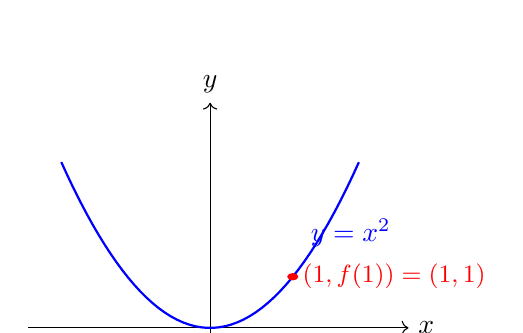
\begin{tikzpicture}[x=1.05cm,y=0.65cm]
  \draw[->] (-2.2,0) -- (2.4,0) node[right] {$x$};
  \draw[->] (0,-0.3) -- (0,4.4) node[above] {$y$};
  \draw[blue,thick,domain=-1.8:1.8,samples=50] plot (\x,{\x*\x});
  \node[blue,above right] at (1.1,1.4) {$y=x^2$};
  \draw[red,fill=red] (1,1) circle (0.06);
  \node[red,right] at (1,1) {\small \((1,f(1))=(1,1)\)};
\end{tikzpicture}
\caption{函数图像只画出满足 \(y=f(x)\) 的点；它不是函数规则的全部替代品。}
\label{fig:function-graph}
\end{figure}

\subsection{数列和极限：无限过程的精确说法}

\begin{definition}[数列]\label{def:sequence}
数列是按正整数编号的一串数，写作
\[
(a_n)_{n\ge1}=a_1,a_2,a_3,\ldots.
\]
也可以把它看成一个函数 \(a:\mathbb N_{\ge1}\to\mathbb R\)，其中 \(a(n)=a_n\)。
下标表示输入编号，不表示乘法。
\end{definition}

\begin{definition}[数列极限]\label{def:sequence-limit}
对数列 \((a_n)\)，写 \(a_n\to L\) 或 \(\lim_{n\to\infty}a_n=L\)，正式意思是：对每个 \(\varepsilon>0\)，都存在正整数 \(N\)，使得只要 \(n\ge N\)，就有
\[
|a_n-L|<\varepsilon.
\]
\(\varepsilon\) 是预先给定的任意小误差，\(N\) 可以依赖于 \(\varepsilon\)，但不能依赖于后来选择的 \(n\)。符号 \(n\to\infty\) 不是说“到达一个叫无穷大的数”，而是说编号可以大到超过任何预先给定的界。
\end{definition}

\begin{figure}[htbp]
\centering
\begin{tikzpicture}[x=0.7cm,y=1cm]
  \draw[->] (0,0) -- (9.3,0) node[right] {$n$};
  \draw[->] (0,0) -- (0,2.0) node[above] {$a_n$};
  \draw[gray,dashed] (0,1.25) -- (9,1.25) node[right] {\small \(L+\varepsilon\)};
  \draw[gray,dashed] (0,0.75) -- (9,0.75) node[right] {\small \(L-\varepsilon\)};
  \draw[blue,thick] plot coordinates {(0.7,0.3) (1.5,1.75) (2.3,0.55) (3.1,1.45) (3.9,0.82) (4.7,1.20) (5.5,0.94) (6.3,1.08) (7.1,0.98) (7.9,1.03) (8.7,1.0)};
  \draw[red,thick] (0,1)--(9,1) node[right] {\small \(L\)};
  \draw[<->,red] (8.9,0.75)--(8.9,1.0) node[midway,right] {\tiny \(\varepsilon\)};
  \node[align=left,text width=4.8cm,below=0.35cm] at (4.7,0) {\small 只要 \(n\) 足够大，所有点都落进\(L\)周围的误差带。};
\end{tikzpicture}
\caption{极限的图像直觉：不是最后一个点等于 \(L\)，而是后面的所有点都能被压进任意窄的带状区域。}
\label{fig:sequence-limit}
\end{figure}

\Needspace{8\baselineskip}
\begin{proposition}[一个最基本的极限]\label{prop:one-over-n-limit}
\[
\lim_{n\to\infty}\frac1n=0.
\]
\end{proposition}

\begin{proof}
给定 \(\varepsilon>0\)，取正整数 \(N>1/\varepsilon\)。当 \(n\ge N\) 时，\(0<1/n\le1/N<\varepsilon\)，所以 \(|1/n-0|<\varepsilon\)。这正是定义中 \(\forall\varepsilon\,\exists N\) 的要求。
\end{proof}

\begin{definition}[函数极限]\label{def:function-limit}
设 \(f\) 至少在 \(a\) 的某个去心邻域有定义。\(\lim_{x\to a}f(x)=L\) 表示对每个 \(\varepsilon>0\)，存在 \(\delta>0\)，使
\[
0<|x-a|<\delta\quad\Longrightarrow\quad |f(x)-L|<\varepsilon.
\]
这里 \(x\) 不必等于 \(a\)，所以函数在 \(a\) 处的值和趋近 \(a\) 时的极限是两个不同问题。
\end{definition}

\begin{figure}[htbp]
\centering
\begin{tikzpicture}[x=0.9cm,y=0.9cm]
  \begin{scope}[xshift=-3.5cm]
    \draw[->] (-2.2,0)--(2.2,0) node[right] {\(x\)};
    \draw[red,very thick] (-0.55,0)--(0.55,0);
    \draw[red,fill=red] (0,0) circle (0.06);
    \draw[<->,blue,thick] (-0.55,-0.35)--(0.55,-0.35)
      node[midway,below,font=\scriptsize] {\(\delta\)};
    \node[figurelabel] at (0,-1.0) {输入端：\(a-\delta<x<a+\delta\)};
    \node[font=\scriptsize] at (0,0.25) {\(a\)};
  \end{scope}
  \draw[diagramarrow] (-1.25,0.2)--(0.15,0.2) node[midway,above,font=\scriptsize] {\(f\)};
  \begin{scope}[xshift=3.0cm]
    \draw[->] (-2.2,0)--(2.2,0) node[right] {\(y\)};
    \draw[blue,very thick] (-0.65,0)--(0.65,0);
    \draw[blue,fill=blue] (0,0) circle (0.06);
    \draw[<->,red,thick] (-0.65,-0.35)--(0.65,-0.35)
      node[midway,below,font=\scriptsize] {\(\varepsilon\)};
    \node[figurelabel] at (0,-1.0) {输出端：\(L-\varepsilon<f(x)<L+\varepsilon\)};
    \node[font=\scriptsize] at (0,0.25) {\(L\)};
  \end{scope}
\end{tikzpicture}
\caption{\(\varepsilon\)-\(\delta\) 的几何读法：先给定输出端的误差带，再寻找输入端足够小的邻域，使函数把它送进误差带。}
\label{fig:epsilon-delta-neighborhood}
\end{figure}

\subsubsection{极限的纪律：唯一性、夹逼、运算与连续性}

前面的定义说明了“趋近”是什么意思，但还没有说明极限为什么可以被计算。
下面四组结果是初学者最常用、也最容易被一句“显然”掩盖的逻辑接口。
它们都建立在同一个量词结构上；因此后文把它们当作正式工具使用时，会明确标出
假设，而不把图形直觉当作证明。

\begin{proposition}[极限的唯一性]\label{prop:sequence-limit-unique}
若实数数列 \((a_n)\) 同时满足 \(a_n\to L\) 和 \(a_n\to M\)，则
\[
L=M.
\]
也就是说，在固定的距离 \(d(x,y)=|x-y|\) 下，一个数列不能有两个不同的极限。
\end{proposition}

\begin{proof}
反设 \(L\ne M\)，取 \(\varepsilon=|L-M|/3>0\)。由 \(a_n\to L\)，存在
\(N_1\)，使 \(n\ge N_1\) 时 \(|a_n-L|<\varepsilon\)；由 \(a_n\to M\)，存在
\(N_2\)，使 \(n\ge N_2\) 时 \(|a_n-M|<\varepsilon\)。当
\(n\ge\max\{N_1,N_2\}\) 时，三角不等式给出
\[
|L-M|\le |L-a_n|+|a_n-M|<2\varepsilon
=\frac23|L-M|,
\]
矛盾。因此 \(L=M\)。
\end{proof}

\begin{proposition}[收敛数列一定有界]\label{prop:convergent-sequence-bounded}
若 \(a_n\to L\)，则存在常数 \(C>0\)，使对所有 \(n\) 都有
\[
|a_n|\le C.
\]
这里“有界”只表示所有项落在某个固定区间 \([-C,C]\) 内，并不表示数列已经收敛到
某个特定值。
\end{proposition}

\begin{proof}
取 \(\varepsilon=1\)，并把相应的 \(N\) 增大到至少 \(2\)。当 \(n\ge N\) 时，
\[
|a_n|\le |a_n-L|+|L|<|L|+1.
\]
前 \(N-1\) 项只有有限多个，令
\[
C=\max\{|a_1|,\ldots,|a_{N-1}|,|L|+1\}.
\]
则尾部和有限个初始项都被同一个 \(C\) 控制，故结论成立。
\end{proof}

\begin{theorem}[夹逼定理]\label{thm:squeeze-sequence}
设三个实数数列满足：存在 \(N_0\)，使得当 \(n\ge N_0\) 时
\[
a_n\le b_n\le c_n,
\]
并且 \(a_n\to L\)、\(c_n\to L\)。那么
\[
b_n\to L.
\]
“最终满足不等式”就足够；前面有限多个 \(n\) 的行为不会改变极限。
\end{theorem}

\begin{proof}
给定 \(\varepsilon>0\)。由 \(a_n\to L\)，存在 \(N_1\)，使
\(n\ge N_1\) 时 \(L-\varepsilon<a_n\)；由 \(c_n\to L\)，存在 \(N_2\)，使
\(n\ge N_2\) 时 \(c_n<L+\varepsilon\)。当
\[
n\ge N=\max\{N_0,N_1,N_2\}
\]
时，合并三组不等式得到
\[
L-\varepsilon<a_n\le b_n\le c_n<L+\varepsilon.
\]
于是 \(|b_n-L|<\varepsilon\)，这正是 \(b_n\to L\) 的定义。
\end{proof}

\begin{proposition}[极限的线性、乘法与商规则]\label{prop:sequence-limit-algebra}
若 \(a_n\to A\)、\(b_n\to B\)，且 \(\lambda\in\mathbb R\)，则
\[
\begin{aligned}
a_n+b_n&\longrightarrow A+B, &
\lambda a_n&\longrightarrow\lambda A,\\
a_nb_n&\longrightarrow AB.
\end{aligned}
\]
若另外 \(B\ne0\)，并且从某一项开始 \(b_n\ne0\)，则
\[
\frac{a_n}{b_n}\longrightarrow\frac AB.
\]
商规则的“分母最终不为零”不是装饰性条件；若分母可以无限接近零，
商可能没有有限极限。
\end{proposition}

\begin{proof}
加法由
\[
|a_n+b_n-(A+B)|\le |a_n-A|+|b_n-B|
\]
和 \(\varepsilon/2\) 的选择直接得到；数乘同理。由
\term{prop:convergent-sequence-bounded}{收敛数列有界}，存在 \(C>0\) 使
\(|b_n|\le C\)。乘法的误差分解为
\[
a_nb_n-AB=b_n(a_n-A)+A(b_n-B).
\]
给定 \(\varepsilon>0\)，令 \(n\) 足够大，使
\[
|a_n-A|<\frac{\varepsilon}{2(C+1)},\qquad
|b_n-B|<\frac{\varepsilon}{2(|A|+1)}.
\]
则
\[
|a_nb_n-AB|
\le C|a_n-A|+|A||b_n-B|<\varepsilon.
\]
最后，\(B\ne0\) 时，\(b_n\to B\) 意味着从某一项开始
\(|b_n-B|<|B|/2\)，所以 \(|b_n|\ge |B|/2\)，并且
\[
\left|\frac1{b_n}-\frac1B\right|
=\frac{|b_n-B|}{|b_n||B|}
\le \frac{2}{|B|^2}|b_n-B|\longrightarrow0.
\]
再将 \(a_n\to A\) 与 \(1/b_n\to1/B\) 代入已经证明的乘法规则，即得商规则。
\end{proof}

\begin{definition}[定义域的聚点]\label{def:domain-accumulation-point}
设 \(D\subseteq\mathbb R\)。点 \(a\in\mathbb R\) 称为 \(D\) 的聚点，如果
\[
\forall\delta>0\ \exists x\in D,\qquad 0<|x-a|<\delta.
\]
它不要求 \(a\in D\)：例如 \(0\) 是 \((0,1)\) 的聚点，但不属于 \((0,1)\)。
这个条件排除了“去心邻域里根本没有定义域点”造成的空洞极限。
\end{definition}

\begin{definition}[点态连续性]\label{def:pointwise-continuity}
设 \(D\subseteq\mathbb R\)，\(f:D\to\mathbb R\)，且 \(a\in D\)。称 \(f\) 在 \(a\)
处连续，如果
\[
\forall\varepsilon>0\ \exists\delta>0\ \forall x\in D,\qquad
|x-a|<\delta\Longrightarrow |f(x)-f(a)|<\varepsilon.
\]
与\term{def:function-limit}{函数极限}相比，这里允许 \(x=a\)，并且输出的比较对象是
函数的实际值 \(f(a)\)，而不是另行给定的 \(L\)。
\end{definition}

\begin{proposition}[极限与连续性的桥接]\label{prop:limit-continuity-bridge}
设 \(a\) 是 \(D\) 的聚点，\(f:D\to\mathbb R\)，且 \(a\in D\)。则
\[
f\text{ 在 }a\text{ 处连续}
\quad\Longleftrightarrow\quad
\lim_{\substack{x\to a\\x\in D}}f(x)=f(a).
\]
这只是把同一个 \(\varepsilon\)--\(\delta\) 条件在 \(x=a\) 与 \(x\ne a\) 两种情形下拆开，
不是把“函数值”和“极限”混成一个新对象。
\end{proposition}

\begin{proof}
若 \(f\) 在 \(a\) 处连续，给定 \(\varepsilon>0\) 取连续性定义中的 \(\delta\)。
当 \(0<|x-a|<\delta\) 时当然也有 \(|x-a|<\delta\)，故
\(|f(x)-f(a)|<\varepsilon\)，于是去心极限等于 \(f(a)\)。

反过来，若去心极限等于 \(f(a)\)，给定 \(\varepsilon>0\) 取相应的 \(\delta\)。
对于 \(x\in D\) 且 \(|x-a|<\delta\)，若 \(x\ne a\)，使用极限条件；
若 \(x=a\)，则 \(|f(x)-f(a)|=0<\varepsilon\)。两种情形合起来正是连续性定义。
\end{proof}

\begin{remark}[一张“极限工具链”]
唯一性告诉我们结果不会依赖于证明路线；夹逼把难算的对象夹在两个易算对象之间；
运算规则允许逐项计算；连续性桥接则说明“先取函数值再逼近”和“先逼近再取值”
在何时一致。四者共同构成从定义到计算的最短闭环。
\end{remark}

\Needspace{15\baselineskip}
\begin{figure}[htbp]
\centering
\begin{tikzpicture}[node distance=0.35cm and 0.55cm]
  \node[routebox,text width=2.35cm] (def) { \(\varepsilon\)--\(N\)\\定义 };
  \node[routebox,text width=2.35cm,right=of def] (unique) {唯一性\\结果不分叉};
  \node[routebox,text width=2.35cm,below=of unique] (squeeze) {夹逼\\控制中间项};
  \node[routebox,text width=2.35cm,left=of squeeze] (algebra) {运算规则\\逐项计算};
  \node[routebox,text width=2.35cm,right=of unique] (continuity) {连续性\\极限等于函数值};
  \draw[diagramarrow] (def)--(unique);
  \draw[diagramarrow] (unique)--(continuity);
  \draw[diagramarrow] (def)--(algebra);
  \draw[diagramarrow] (def)--(squeeze);
  \draw[diagramarrow] (algebra)--(continuity);
  \draw[diagramarrow] (squeeze)--(continuity);
\end{tikzpicture}
\caption{极限的四个工作接口：每个箭头表示“在相应假设下可以调用”，不表示四条结果彼此等价。}
\label{fig:limit-property-chain}
\end{figure}

\subsection{坐标、向量和距离：把图形变成可计算对象}

\begin{definition}[坐标]\label{def:coordinate}
平面坐标把一个点写成有序对 \((x,y)\in\mathbb R^2\)。有序很重要：通常 \((x,y)\ne(y,x)\)。
更一般地，\(\mathbb R^n\) 中的点由 \(n\) 个坐标组成，写成 \((x_1,\ldots,x_n)\)。
\end{definition}

\begin{definition}[向量]\label{def:vector}
在选定坐标后，从原点指向点 \((x,y)\) 的箭头可看成向量
\[
v=\begin{pmatrix}x\\y\end{pmatrix}.
\]
向量可以逐坐标相加，也可以乘实数；它表示位移或方向，而不是一个固定位置。
\end{definition}

\begin{definition}[欧氏距离]\label{def:distance}
对向量 \(v=(x,y)\)，其欧氏长度（范数）为
\[
\|v\|=\sqrt{x^2+y^2},
\]
两点 \(p=(x_1,y_1)\)、\(q=(x_2,y_2)\) 的距离为
\[
d(p,q)=\|q-p\|=\sqrt{(x_2-x_1)^2+(y_2-y_1)^2}.
\]
距离是两个点之间的数；向量 \(q-p\) 是从 \(p\) 指向 \(q\) 的位移。二者相关，但对象类型不同。
\end{definition}

\begin{figure}[htbp]
\centering
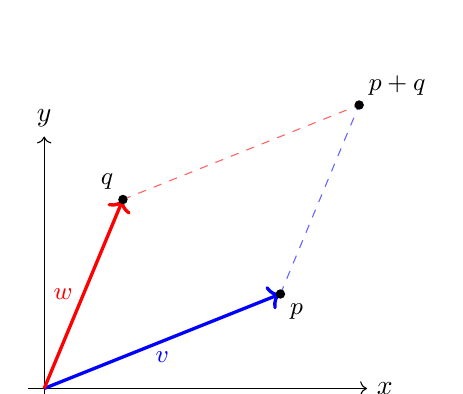
\begin{tikzpicture}[x=1cm,y=1cm]
  \draw[->] (-0.2,0) -- (4.1,0) node[right] {$x$};
  \draw[->] (0,-0.2) -- (0,3.2) node[above] {$y$};
  \draw[->,blue,very thick] (0,0)--(3,1.2) node[midway,below] {\small \(v\)};
  \draw[->,red,very thick] (0,0)--(1,2.4) node[midway,left] {\small \(w\)};
  \draw[blue!60,dashed] (3,1.2)--(4,3.6);
  \draw[red!60,dashed] (1,2.4)--(4,3.6);
  \fill (3,1.2) circle (0.06) node[below right] {\small \(p\)};
  \fill (1,2.4) circle (0.06) node[above left] {\small \(q\)};
  \fill (4,3.6) circle (0.06) node[above right] {\small \(p+q\)};
\end{tikzpicture}
\caption{向量相加可以画成平行四边形的对角线；坐标把几何关系转成代数计算。}
\label{fig:vector-addition}
\end{figure}

\subsection{矩阵：数字表格如何变成变换}

\Needspace{10\baselineskip}
\begin{definition}[矩阵的读法]\label{def:matrix-read}
一个 \(m\times n\) 矩阵是一个有 \(m\) 行、\(n\) 列的数字表格，写作
\[
A=(a_{ij})=\begin{pmatrix}
a_{11}&\cdots&a_{1n}\\
\vdots&&\vdots\\
a_{m1}&\cdots&a_{mn}
\end{pmatrix}.
\]
\(a_{ij}\) 是第 \(i\) 行第 \(j\) 列的数。矩阵可以乘向量；例如
\[
\begin{pmatrix}a&b\\c&d\end{pmatrix}
\begin{pmatrix}x\\y\end{pmatrix}
=\begin{pmatrix}ax+by\\cx+dy\end{pmatrix}.
\]
因此一个矩阵可以把平面中的点/向量送到另一个点/向量。矩阵相乘表示连续做两个线性变换；单位矩阵表示“不改变”，可逆矩阵表示存在一个变换可以撤回。行列式、可逆性的完整定义和群结构在模块二正式展开。
\end{definition}

\begin{figure}[htbp]
\centering
\begin{tikzpicture}[x=1.05cm,y=1.05cm]
  \draw[->] (-0.2,0)--(2.7,0);
  \draw[->] (0,-0.2)--(0,2.6);
  \draw[gray!60] (0,0)--(1,0)--(1,1)--(0,1)--cycle;
  \node[align=center] at (0.5,-0.35) {\small 原来的\\\small 单位正方形};
  \draw[blue,very thick] (0,0)--(1.7,0.3)--(2.2,1.7)--(0.5,1.4)--cycle;
  \node[blue,align=center] at (1.35,1.85) {\small 矩阵作用后的\\\small 平行四边形};
  \draw[->,thick] (1.1,-0.9)--(1.65,-0.9) node[midway,below] {\small \(A\)};
\end{tikzpicture}
\caption{矩阵的几何意义：它把基向量决定的单位正方形送到由两列向量张成的平行四边形。}
\label{fig:matrix-action}
\end{figure}

\subsection{导数与积分：局部变化和整体累积}

\begin{definition}[导数]\label{def:derivative}
若函数 \(u\) 在 \(x_0\) 附近有定义，\(u\) 在 \(x_0\) 处的导数是差商的极限
\[
u'(x_0)=\lim_{h\to0}\frac{u(x_0+h)-u(x_0)}h,
\]
其中 \(h\) 是一个趋近于零但不等于零的小位移。它表示曲线在 \(x_0\) 处的瞬时变化率，也就是切线斜率。多变量函数的导数会把一个输入方向的变化率组织成线性映射；这就是后文 \(DF\) 和 \(dF_p\) 的来源。
\end{definition}

\begin{definition}[积分]\label{def:integral}
定积分
\[
\int_a^b u(x)\,dx
\]
可以先理解为把区间 \([a,b]\) 切成很多小段，把每段的“高度\(\times\)宽度”相加，再让小段宽度趋于零的极限。它是带方向的累积量：若 \(u\) 在横轴下方，贡献为负。严格的 Riemann 积分和曲线积分会在模块三、五中分别说明。
\end{definition}

\begin{figure}[htbp]
\centering
\begin{tikzpicture}[x=0.85cm,y=0.72cm]
  \draw[->] (-0.2,0)--(7.2,0) node[right] {$x$};
  \draw[->] (0,-0.2)--(0,3.6) node[above] {$y$};
  \draw[blue,thick,domain=0.2:6.7,samples=50] plot (\x,{0.25+0.18*\x+0.05*\x*\x});
  \foreach \x in {1,2,3,4,5,6}
    \draw[blue!35,fill=blue!10] (\x,0) rectangle (\x+0.8,{0.25+0.18*(\x+0.4)+0.05*(\x+0.4)*(\x+0.4)});
  \node[align=center] at (3.5,-0.65) {\small 矩形面积相加\\\small \(\longrightarrow\) 积分};
  \draw[red,thick] (2.8,1.5)--(4.0,2.25);
  \node[red,above] at (3.8,2.2) {\small 切线斜率 \(u'(x_0)\)};
\end{tikzpicture}
\caption{导数看一个点附近的局部斜率，积分把许多小贡献累积成整体量。}
\label{fig:derivative-integral}
\end{figure}

\begin{remark}[本模块的核心翻译表]
\[
\begin{array}{c|c|c}
\text{符号} & \text{普通话} & \text{后文用途}\\
\hline
\varepsilon,\delta & \text{允许的误差和输入范围} & \text{极限、连续、复导数}\\
\|v\|,d(p,q) & \text{长度和两点距离} & \text{度量空间、拟共形畸变}\\
A v & \text{矩阵对向量的作用} & \text{群作用、坐标变化、Jacobian}\\
u'(x) & \text{局部变化率} & \text{全纯函数、曲率、变形}\\
\int u\,dx & \text{连续累积} & \text{Green、Stokes、周期}\\
\end{array}
\]
同一个符号可能在不同章节有更高级的版本，但每次都要回到“对象类型”来判断含义。
\end{remark}

\subsection{练习与出口检查}

\paragraph{基础练习。}
\begin{enumerate}[label=M0.\arabic*.]
  \item 把 \(\{x\in\mathbb R:-2\le x<3\}\) 写成区间记号，并在数轴上标出两个端点。
  \item 判断 \(\mathbb Q\subseteq\mathbb R\) 和 \(\mathbb R\subseteq\mathbb Q\) 哪一个正确，并说明 \(\sqrt2\) 在哪里。
  \item 把“存在一个正整数 \(N\)，使所有 \(n\ge N\) 都满足 \(|a_n-L|<\varepsilon\)”翻译成含有 \(\exists,\forall\) 的句子。
  \item 计算 \(\begin{pmatrix}1&2\\0&1\end{pmatrix}\begin{pmatrix}x\\y\end{pmatrix}\)，并解释它对平面点做了什么。
  \item 对 \(u(x)=x^2\)，用差商写出 \(u'(1)\)，先不要急于计算极限；指出其中的输入变化量是什么。
  \item 分别判断 \(x^2:\mathbb R\to\mathbb R\)、\(x^2:\mathbb R\to[0,\infty)\) 和
    \(x^3:\mathbb R\to\mathbb R\) 的单射性、满射性和双射性，并指出陪域在哪里改变了结论。
  \item 设 \(X\ne\varnothing\)、\(Y\ne\varnothing\)，判断投影
    \(\pi_1:X\times Y\to X\) 何时单射、何时满射；再说明 \(X=\varnothing\) 时为什么要单独讨论。
  \item 设 \(f:X\to Y\) 且 \(X,Y\) 都有限并满足 \(|X|=|Y|=4\)。若已知 \(f\) 是单射，能否
    直接断定它满射？若已知它不是满射，能否断定它不是单射？说明所用定理的前提。
  \item 判断是否存在单射 \(\{1,2,3,4\}\to\{a,b,c\}\)，并用“碰撞”语言说明理由；再判断
    是否存在满射 \(\{1,2,3\}\to\{a,b,c,d\}\)。
  \item 分别判断
    \[
    u:\mathbb Z\to\mathbb Z,\ n\mapsto 2n,\qquad
    v:\mathbb Z\to\mathbb N,\ n\mapsto |n|,\qquad
    w:[0,\infty)\to[0,\infty),\ x\mapsto x^2
    \]
    是单射、满射还是双射；每一个判断都写出一个证明或一个反例。
  \item 对任意 \(f:X\to Y\)，令 \(I=f(X)\)。写出
    \(X\to I\to Y\) 的两个映射，并说明哪一步自动满射、哪一步自动单射。
    再对 \(f(x)=x^2:\mathbb R\to\mathbb R\) 指出“碰撞”和“遗漏”分别发生在哪里。
  \item 对 \(f:\mathbb R\to[0,\infty)\)、\(f(x)=x^2\)，判断它是否有左逆或右逆；
    再对 \(g:[0,\infty)\to[0,\infty)\)、\(g(x)=x^2\)，写出其唯一的左逆和右逆。
  \item 设 \(a_n\to L\) 且 \(a_n\to M\)。用 \(\varepsilon/3\) 的方法证明
    \(L=M\)，并说明为什么“极限唯一”不是定义本身，而是由定义推出的命题。
  \item 设 \(a_n=-1/n\)、\(b_n=\sin n/n\)、\(c_n=1/n\)。验证最终不等式
    \(a_n\le b_n\le c_n\)，再用夹逼定理求 \(\lim b_n\)。
  \item 不展开高次乘法，直接用极限运算规则计算
    \[
    \lim_{n\to\infty}\left(2+\frac1n\right)\left(3-\frac2n\right).
    \]
    指出其中哪一步使用了“收敛数列有界”。
  \item 设
    \[
    f(x)=\begin{cases}x^2,&x\ne1,\\ 7,&x=1.\end{cases}
    \]
    计算 \(\lim_{x\to1}f(x)\)，并判断 \(f\) 在 \(1\) 处是否连续；说明“极限存在”
    与“连续”为什么不是同一句话。
  \item 说明数列 \(a_n=(-1)^n\) 不收敛。提示：若它收敛，偶数项和奇数项分别应该
    收敛到什么；也可以直接选择一个固定的 \(\varepsilon\) 制造矛盾。
\end{enumerate}

\Needspace{18\baselineskip}
\begin{answerkey}
M0.1 的区间是 \([-2,3)\)：\(-2\) 处用实心端点，\(3\) 处用空心端点。
M0.2 中只有 \(\mathbb Q\subseteq\mathbb R\) 正确；\(\sqrt2\in\mathbb R\setminus\mathbb Q\)。
M0.3 应写成
\(\exists N\in\mathbb N\,\forall n\in\mathbb N,\,
(n\geq N\Rightarrow |a_n-L|<\varepsilon)\)。
M0.4 的矩阵把 \((x,y)\) 送到 \((x+2y,y)\)，是沿水平方向的剪切。
M0.5 的差商是 \(((1+h)^2-1)/h=2+h\)，输入变化量就是 \(h\)，极限为 \(2\)。
M0.6 第一个既不单射也不满射；第二个满射但不单射；第三个是双射。差别来自陪域以及公式本身的单调性/值域。
M0.7 在 \(X,Y\) 都非空时，\(\pi_1\) 总是满射；它单射当且仅当 \(Y\) 只有一个元素。
若 \(Y\) 有两个不同元素 \(y_1,y_2\)，取任意 \(x\in X\)，则
\(\pi_1(x,y_1)=\pi_1(x,y_2)\)，所以不单射。若 \(X=\varnothing\)，投影是
\(\varnothing\to\varnothing\)，自动是双射。
M0.8 在有限且等势的前提下，单射、满射、双射等价，所以已知单射可断定满射；已知不是满射，
也可由这组三者等价关系反向推出不是单射。这里必须用到 \(|X|=|Y|<\infty\)。
M0.9 不存在从四元素集合到三元素集合的单射；四个输入若都不碰撞就需要四个不同输出，
但陪域只有三个元素。不存在从三元素集合到四元素集合的满射，因为至少有一个目标元素没有原像。
M0.10 \(u\) 是单射但不是满射：\(u(n)=u(m)\) 给出 \(2n=2m\)，故 \(n=m\)；但奇数没有原像。
\(v\) 是满射但不是单射：每个 \(k\in\mathbb N\) 都有 \(v(k)=k\)，但
\(v(1)=v(-1)\)。\(w\) 是双射：它单调递增，故单射；任意 \(y\geq0\) 都有唯一
\(x=\sqrt y\geq0\)，故满射。
M0.11 令 \(I=f(X)\)，则
\(\widetilde f:X\to I,\ x\mapsto f(x)\) 自动满射，包含映射
\(\iota:I\hookrightarrow Y,\ u\mapsto u\) 自动单射，并且
\(f=\iota\circ\widetilde f\)。对 \(x^2:\mathbb R\to\mathbb R\)，第一步中
\(1,-1\) 碰撞，第二步中每个负数都被陪域允许但没有原像。
M0.12 \(f\) 不是单射，所以没有左逆；但它是满射，取
\(s(y)=\sqrt y\) 即有 \(f\circ s=\operatorname{id}_{[0,\infty)}\)，所以它有右逆。
\(g\) 是双射，且 \(g^{-1}(y)=\sqrt y\) 同时是唯一左逆和唯一右逆。
M0.13 取 \(\varepsilon=|L-M|/3\)。两个收敛条件在同一个足够大的 \(n\) 上同时成立，
三角不等式会给出 \(|L-M|<2|L-M|/3\)，矛盾，所以 \(L=M\)。
这说明唯一性是定理，而不是把“极限”一词换一种写法。
M0.14 因为 \(-1\le\sin n\le1\)，所以
\(-1/n\le\sin n/n\le1/n\)，两端都趋于 \(0\)，故中间数列也趋于 \(0\)。
M0.15 由 \(1/n\to0\) 和极限运算规则，
\[
\left(2+\frac1n\right)\left(3-\frac2n\right)\longrightarrow2\cdot3=6.
\]
乘法误差证明中需要知道 \(3-2/n\) 这一因子有界；这正是收敛数列有界命题的作用。
M0.16 去心邻域内 \(f(x)=x^2\)，故 \(\lim_{x\to1}f(x)=1\)，但 \(f(1)=7\)，
所以 \(f\) 在 \(1\) 处不连续。极限只看 \(x\ne1\) 的附近，连续性还要求贴合实际值。
M0.17 偶数项恒为 \(1\)，奇数项恒为 \(-1\)。若全数列收敛，两个子列必须有相同极限，
但这里分别为 \(1\) 和 \(-1\)，故不收敛；也可取 \(\varepsilon=1/2\) 直接违反定义。
自检时必须同时说出端点、量词、映射的定义域/陪域、向量坐标和矩阵输入输出，不能只给最后数值。
\end{answerkey}

\paragraph{出口检查。}
读者若能回答下面五句话，便可以进入模块一：
\[
\begin{gathered}
\text{开区间为什么不包括端点}\qquad
\text{“}\lim a_n=L\text{”为什么不要求某个 }a_n\text{ 等于 }L\\
\text{极限为什么唯一}\qquad
\text{什么时候可以使用夹逼定理}\qquad
\text{函数极限何时等于函数值}\\
\text{点和向量有什么不同}\qquad
\text{矩阵为什么可以看成变换}\qquad
\text{导数和积分分别看局部还是整体}
\end{gathered}
\]
如果暂时答不出，不必回到整本书，只回到本模块对应的小节和图~\ref{fig:intervals}、
图~\ref{fig:sequence-limit}、图~\ref{fig:limit-property-chain}、图~\ref{fig:matrix-action}。

\clearpage
\section{模块一：集合、函数与“什么算相同”}

\moduleguide{只需会读集合、函数和简单证明；不要求先学抽象代数。}{会区分对象、结构、映射和等价关系，并能解释为什么要构造商。}{能用自己的话说明“同态、同构、同胚、同伦”比较的对象分别是什么。}

\subsection{从函数到数学对象}

函数 \(f(x)=x^2\) 把输入 \(x\) 送到输出 \(x^2\)。抽象数学保留这个“输入--输出”思想，但允许输入和输出是点、曲线、矩阵、集合甚至另一个函数。

\begin{remark}[集合与函数的回收]
模块零已经正式定义集合上的映射、定义域、陪域、像集、单射、满射、双射及逆映射。
本模块把这些对象放进“什么算相同”的框架中；之后的群同态、同构、同胚和同伦，
都是在增加结构或改变比较层次。
\end{remark}

\begin{example}[投影、包含与常值映射]
若 \(X\ne\varnothing\) 且 \(Y\ne\varnothing\)，第一投影
\[
\pi_1:X\times Y\longrightarrow X,\qquad \pi_1(x,y)=x
\]
是满射；在当前的非空假设下，它当且仅当 \(Y\) 只有一个元素时是单射。包含映射
\[
\iota:A\hookrightarrow B,\qquad \iota(a)=a
\]
总是单射，但只有 \(A=B\) 时才是满射。若 \(X\ne\varnothing\)，常值映射
\(c:X\to Y\) 的像集只有一个点，因此除非 \(Y\) 只有一个元素，否则它不是满射；
除非 \(X\) 至多有一个元素，否则它不是单射。它们把量词定义变成了可以直接画出的模型。
若不假设 \(X\ne\varnothing\)，则 \(X=\varnothing\) 时投影是空映射，需按空集边界单独判断。
\end{example}

\begin{remark}[复合与恒等映射已在模块零定义]\label{rem:function-composition-recall}
函数复合与恒等映射已经在模块零的
\term{def:function-composition}{正式定义}中给出。本模块只反复使用它们，不再重复定义：
复合按“先右后左”读取，恒等映射什么也不改变。
\end{remark}

\begin{definition}[限制映射]\label{def:restriction-map}
设 \(f:X\to Y\)，\(A\subseteq X\)。把输入限制在 \(A\) 上得到
\[
f|_A:A\to Y,\qquad f|_A(a)=f(a),
\]
称为 \(f\) 在 \(A\) 上的\term{def:restriction-map}{限制映射}。它改变了定义域，通常也会改变满射性；
若原来的 \(f\) 单射，则 \(f|_A\) 仍单射，但即使 \(f\) 满射，\(f|_A\) 也可能不满射。
\end{definition}

\begin{definition}[包含映射]\label{def:inclusion-map}
设 \(A\subseteq X\)。子集 \(A\) 到 \(X\) 的\term{def:inclusion-map}{包含映射}是
\[
\iota_A^X:A\to X,\qquad \iota_A^X(a)=a.
\]
它总是单射；只有当 \(A=X\) 时才是满射。
\end{definition}

\begin{definition}[陪域缩小]\label{def:codomain-restriction}
设 \(f:X\to Y\)，且 \(f(X)\subseteq B\subseteq Y\)。同一条规则的\term{def:codomain-restriction}{陪域缩小}
是
\[
f_B:X\to B,\qquad f_B(x)=f(x).
\]
它不会改变输入或输出的实际数值，却可能改变“是否满射”的答案，因为满射总是
相对于当前写出的陪域 \(B\) 判断。最小的合法陪域是像集 \(f(X)\)。
\end{definition}

\begin{remark}[三种改变映射声明的操作]
限制映射改变定义域，包含映射把一个子集作为定义域嵌入较大的陪域，陪域缩小改变陪域；
它们都可能保持原来的计算规则，但不是同一个操作。后面的性质表分别说明它们如何影响
单射与满射。
\end{remark}

\begin{proposition}[限制与陪域缩小的基本性质]
设 \(f:X\to Y\)、\(A\subseteq X\)，且 \(f(X)\subseteq B\subseteq Y\)。则
\[
\begin{array}{c}
f\text{ 单射}\Longrightarrow f|_A\text{ 单射},\\[0.2em]
f_B\text{ 满射}\Longleftrightarrow f(X)=B,\\[0.2em]
f_B\text{ 单射}\Longleftrightarrow f\text{ 单射}.
\end{array}
\]
特别地，\(f|_A\) 是否满射要比较 \(f(A)\) 与 \(Y\)，而 \(f_B\) 是否满射要比较
\(f(X)\) 与新陪域 \(B\)；两者改变的是不同一端的类型数据。
\end{proposition}

\begin{proof}
若 \(f|_A(a_1)=f|_A(a_2)\)，则 \(f(a_1)=f(a_2)\)，由 \(f\) 单射得
\(a_1=a_2\)。由满射定义，\(f_B\) 满射正好意味着每个 \(b\in B\) 都属于
\(f(X)\)，即 \(f(X)=B\)。陪域缩小不改变公式和定义域，所以 \(f_B\) 与 \(f\)
具有相同的碰撞关系，单射性等价。
\end{proof}

\begin{proposition}[复合的结合律]
若 \(f:X\to Y\)、\(g:Y\to Z\)、\(h:Z\to W\)，则
\[
h\circ(g\circ f)=(h\circ g)\circ f.
\]
\end{proposition}

\begin{proof}
对每个 \(x\in X\)，两边都等于 \(h(g(f(x)))\)。函数相等的意思是定义域相同且每个输入的输出都相同。
\end{proof}

\begin{figure}[htbp]
\centering
\begin{tikzpicture}[node distance=0.42cm and 0.72cm]
  \node[conceptbox,minimum width=2.0cm] (x) {\(x\in X\)\\输入};
  \node[conceptbox,right=of x,minimum width=2.0cm] (y) {\(f(x)\in Y\)\\中间结果};
  \node[conceptbox,right=of y,minimum width=2.0cm] (z) {\(g(f(x))\in Z\)\\最终输出};
  \draw[diagramarrow] (x) -- node[above,font=\scriptsize] {\(f\)} (y);
  \draw[diagramarrow] (y) -- node[above,font=\scriptsize] {\(g\)} (z);
  \draw[lightarrow,dashed,bend left=32] (x.north) to node[above,font=\scriptsize] {\(g\circ f\)} (z.north);
  \node[figurelabel,below=0.32cm of y] {复合映射把多步流程压缩成一条箭头；箭头方向决定先后顺序};
\end{tikzpicture}
\caption{函数复合的流程图：先应用 \(f\)，再应用 \(g\)，结果才是 \(g\circ f\)。}
\label{fig:function-composition-flow}
\end{figure}

\begin{remark}[结构和保持结构的路线预览]\label{rem:structure-map-overview}
在集合上额外指定的运算、距离、拓扑、坐标或复坐标规则称为结构。若一个映射保持正在讨论的结构，就称为相应类别中的结构保持映射。这里先只记住这个总原则；群同态、线性映射、同胚和全纯映射的正式条件将在各自模块中给出。因此本段是路线预览，不把后文术语假装成已经完成的定义。
\end{remark}

\begin{remark}[直积在本模块中的回收]
前面的笛卡尔积定义是后文二元关系和同伦的基础。这里再次使用它时，
\(R\subseteq X\times X\) 表示“关系是有序对的集合”，而
\(X\times[0,1]\) 表示“点加时间”的参数空间；不再把直积当作新对象重新定义。
\end{remark}

\begin{center}
{\small
\begin{tabularx}{\textwidth}{p{0.22\textwidth}p{0.30\textwidth}X}
\toprule
对象上增加的结构 & 常见的保持结构的映射 & 这一层主要关心什么 \\
\midrule
只给集合 & 任意函数 & 输入和输出如何对应 \\
代数运算（群、环、模） & 同态 & 运算、单位元和标量作用是否被保持 \\
拓扑（开集、邻域） & 连续映射、同胚 & 哪些性质在连续变形下不变 \\
光滑结构 & 光滑映射、微分同胚 & 能否求导、比较切向量和曲率 \\
复结构 & 全纯映射、双全纯映射 & 哪些坐标变化尊重复分析 \\
\bottomrule
\end{tabularx}
}
\end{center}

这张表不是把不同理论排成一条“谁更真实”的等级，而是说明：每增加一层结构，就增加一批可提问的问题，也增加一批必须保持的条件。

\begin{remark}[同态、同构、同胚与同伦的路线预览]\label{rem:basic-equivalences}
下面四个词都含有“相同”的意味，但它们比较的对象、保持的信息和逻辑层次不同。此处只给阅读地图；
群同态的正式公式在模块二，连续映射和同胚的正式定义已在模块三， 同伦的正式定义在模块四。

\begin{description}[leftmargin=3.2cm,style=nextline]
  \item[同态（homomorphism）]
  若两个对象带有同一种运算，映射只需保持这些运算，就称为同态。它不要求单射或满射，因此可能把不同元素合并，也可能没有覆盖整个目标；正式群论例子见模块二。

  \item[同构（isomorphism）]
  在一个指定的结构类别中，双射且正向、逆向都保持该类别结构的映射称为同构。
  对只含运算的代数类别，逆向保持性可由双射和正向保持性证明；对拓扑、光滑和复解析类别，
  则必须明确检查逆映射的连续、光滑或全纯性。这里“同构”不是脱离背景的词：必须先说明保持的是群运算、环运算、线性结构还是别的结构。

  \item[同胚（homeomorphism）]
  在拓扑空间中，双射若连续且逆映射也连续，就称为同胚。同胚保持开集、邻域、连通性和洞的拓扑信息，但一般不保持距离、角度或曲率；正式定义见模块四。

  \item[同伦（homotopy）]
  同伦首先比较两个映射，而不是两个点集：它允许一个映射随时间参数连续变成另一个映射。同伦等价比同胚更粗，记录可连续收缩的整体形状；正式的参数映射和端点条件见模块四。
\end{description}
\end{remark}

\begin{remark}[四个词的关系不能混用]
可以把四个概念放在下面的“保持信息”表中。表中的“强”不是严格的全序，而是提醒我们：不同类别的结构没有一个自动适用的共同标准。

\begin{center}
{\setlength{\tabcolsep}{3pt}
\begin{tabular}{p{0.18\textwidth}|p{0.27\textwidth}|p{0.25\textwidth}|p{0.20\textwidth}}
\toprule
词语 & 比较的对象 & 需要保持什么 & 是否要求可逆 \\
\midrule
同态 & 代数对象之间的映射 & 运算与单位元等代数规则 & 不要求 \\
同构 & 同一结构类别中的对象 & 该类别的全部指定结构 & 要求双射；正、逆两向都保持结构 \\
同胚 & 拓扑空间之间的映射 & 连续性和拓扑结构 & 要求连续双射且逆连续 \\
同伦 & 两个连续映射之间的变形 & 变形过程的连续性 & 不要求每个中间映射可逆 \\
\bottomrule
\end{tabular}
}
\end{center}

例如，圆盘与一点同伦等价，却不可能同胚：圆盘有许多点，而一点只有一个点。另一方面，两个同胚的曲面未必已经配备了同样的黎曼度量；两个双全纯同构的黎曼曲面则还要求复结构也被保持。以后遇到“相同”时，必须先问：是在代数、拓扑、光滑、度量还是复解析类别中相同？
\end{remark}

\paragraph{读图与读式的习惯。}
“\(f:X\to Y\) 是同态”只说明 \(f\) 保持指定运算；“\(f\) 是同构”还要补充双射，
并按类别检查逆映射的结构保持性；“\(f\) 是同胚”则把运算换成拓扑，并要求连续性及逆连续性；
“\(f_0\simeq f_1\)”的对象是两张箭头，而不是一张箭头。这个句法差别会在基本群、映射类群和
Teichmüller 空间中反复出现。

\subsection{等价关系和商}

如果两种画法只差一个不重要的选择，我们希望把它们归为一类。

\begin{definition}[二元关系]\label{def:relation}
设 \(X\) 是集合。\(X\) 上的一个\term{def:relation}{二元关系}是笛卡尔积
\(X\times X\) 的子集 \(R\subseteq X\times X\)；写作 \(xRy\) 表示
\((x,y)\in R\)。因此，“\(x\) 与 \(y\) 相关”并不是一句模糊的语言，
而是一个可以检验真假的命题。
\end{definition}

\begin{definition}[关系的三种基本性质]\label{def:relation-properties}
设 \(R\subseteq X\times X\) 是集合 \(X\) 上的二元关系。我们分别说：
\begin{enumerate}[label=(\alph*)]
  \item \(R\) \textbf{自反}，如果 \(\forall x\in X,\ xRx\)；
  \item \(R\) \textbf{对称}，如果 \(\forall x,y\in X,\ xRy\Rightarrow yRx\)；
  \item \(R\) \textbf{传递}，如果 \(\forall x,y,z\in X,\ (xRy\land yRz)\Rightarrow xRz\)。
\end{enumerate}
这三条是可以分别检验的性质；一个关系可以满足其中一条或两条，却不满足另外一条。
\end{definition}

\begin{remark}[关系与函数不是同一类对象]
关系 \(R\subseteq X\times X\) 只回答“两个元素是否相关”，同一个 \(x\) 可以与零个、一个或
多个 \(y\) 相关；它不要求给出唯一输出。函数 \(f:X\to Y\) 则是有序对集合
\(\Gamma_f\subseteq X\times Y\) 的特殊情形：每个 \(x\in X\) 恰好对应一个 \(y\in Y\)。
因此，函数可以看作一种特殊关系，但一般关系不是函数。关系的自反、对称、传递性也
分别是关于输入对、交换顺序和三段链的条件，不能与函数的单值性或单射性混用。
\end{remark}

\begin{definition}[等价关系]\label{def:equivalence}
集合 \(X\) 上的关系 \(\sim\) 若对所有 \(x,y,z\in X\) 满足
\[
\underbrace{x\sim x}_{\text{自反性}},\qquad
\underbrace{x\sim y\Rightarrow y\sim x}_{\text{对称性}},\qquad
\underbrace{(x\sim y\ \text{且}\ y\sim z)\Rightarrow x\sim z}_{\text{传递性}},
\]
分别称为自反性、对称性和传递性；满足三者就叫\term{def:equivalence}{等价关系}。
\end{definition}

\begin{example}[同一个集合上的关系可以保留不同信息]
在 \(X=\{1,2,3\}\) 上考虑四种关系：
\[
\begin{array}{c|c|c|c|c}
\text{关系}&\text{自反}&\text{对称}&\text{传递}&\text{它表达的意思}\\
\hline
x=y&\text{是}&\text{是}&\text{是}&\text{只把同一个元素视为相同}\\
\text{任意 }xRy&\text{是}&\text{是}&\text{是}&\text{把所有元素视为同一类}\\
x\le y&\text{是}&\text{否}&\text{是}&\text{有方向的大小比较}\\
|x-y|\le1&\text{是}&\text{是}&\text{否}&\text{相近，但相近不一定可传递}
\end{array}
\]
前两种是等价关系，分别产生三个单元素类和一个三元素类；后两种不是等价关系，
所以不能直接把它们的“相关对象”当作等价类分割。这个表说明“关系”是总容器，
等价关系只是其中特别适合做分类的一种。
\end{example}

\begin{definition}[等价类与代表元]\label{def:equivalence-class}\label{def:representative}
现在设 \(\sim\) 已经是 \(X\) 上的\term{def:equivalence}{等价关系}，且 \(x\in X\)。定义
\[
[x]_{\sim}:=\{y\in X:y\sim x\}
\]
为 \(x\) 的\term{def:equivalence-class}{等价类}。类中的任意元素都称为这个类的一个
\term{def:representative}{代表元}。代表元只是“用来写出这个类的一个成员”，不是理论选出的唯一元素；
若 \(y\sim x\)，那么 \(x\) 与 \(y\) 是同一个等价类的两个代表元。
\end{definition}

\begin{definition}[幂集与集合的分割]\label{def:power-set}\label{def:partition}
集合 \(X\) 的\term{def:power-set}{幂集}是所有 \(X\) 的子集组成的集合：
\[
\mathcal P(X):=\{A:A\subseteq X\}.
\]
一个子集族 \(\mathcal B\subseteq\mathcal P(X)\) 称为 \(X\) 的一个\term{def:partition}{分割}
（或划分），如果满足：
\begin{enumerate}[label=(\alph*)]
  \item 每个块 \(B\in\mathcal B\) 都非空；
  \item 每个元素都被覆盖，即 \(\displaystyle\bigcup_{B\in\mathcal B}B=X\)；
  \item 不同块不重叠，即 \(B,C\in\mathcal B\) 且 \(B\cap C\ne\varnothing\) 时必有 \(B=C\)。
\end{enumerate}
\(\mathcal B\) 中的元素称为块。第二条说没有遗漏，第三条说没有重复归类。
当 \(X=\varnothing\) 时，空的子集族 \(\mathcal B=\varnothing\) 按上述约定是空集的分割；
对非空 \(X\)，分割至少含有一个非空块。这里的“分割”是集合论对象，不是把
\(X\) 切成几何图形；几何切割只是帮助形成直观的例子。
\end{definition}

\begin{definition}[商集与商映射]\label{def:quotient}\label{def:quotient-map}
设 \(\sim\) 是集合 \(X\) 上的等价关系。所有等价类组成\term{def:quotient}{商集}
\[
X/{\sim}=\{[x]_{\sim}:x\in X\}.
\]
商集的元素不是原来的单个 \(x\)，而是整个等价类。把 \(x\) 送到它的等价类的映射
\[
q:X\longrightarrow X/{\sim},\qquad q(x)=[x]_{\sim},
\]
称为\term{def:quotient-map}{商映射}。它忘掉的是“同一类内选了哪个代表元”，保留的是代表元所属的类。
等价关系的等价类会形成 \(X\) 的一个分割；这是后面的正式命题，而不是商集定义中额外假定的条件。
\end{definition}

\begin{definition}[模 \(n\) 的整数商集]\label{def:integer-quotient}
设 \(n\ge1\) 是正整数。在 \(\mathbb Z\) 上定义
\[
a\sim_n b
\quad\Longleftrightarrow\quad
a\equiv b\pmod n
\quad\Longleftrightarrow\quad
n\mid(a-b).
\]
这就是“相差 \(n\) 的整数倍”。后面的命题会验证它是等价关系；其等价类商集记为
\[
\mathbb Z/n\mathbb Z:=\mathbb Z/{\sim_n},
\]
并把 \(a\) 所在的类写作 \([a]\)。因此 \(\mathbb Z/n\mathbb Z\) 的元素是余数类，
不是单个整数；例如 \([a]=[a+n]\)。
\end{definition}

\begin{proposition}[等价关系与集合分割的对应]\label{prop:equivalence-partition-correspondence}
若 \(\sim\) 是 \(X\) 上的等价关系，则
\[
\mathcal B_\sim=\{[x]_\sim:x\in X\}
\]
是 \(X\) 的一个分割。反过来，若 \(\mathcal B\) 是 \(X\) 的一个分割，定义
\[
x\sim_{\mathcal B}y
\quad\Longleftrightarrow\quad
\text{存在 }B\in\mathcal B\text{ 使 }x\in B\text{ 且 }y\in B,
\]
则 \(\sim_{\mathcal B}\) 是等价关系，而且它的等价类恰好是 \(\mathcal B\) 的各个块。
因此，给出等价关系与给出“把 \(X\) 分成互不重叠的块”是同一份信息的两种编码；
商集 \(X/{\sim}\) 可以看作这些块组成的集合。
\end{proposition}

\begin{proof}
先设 \(\sim\) 是等价关系。自反性给出每个 \(x\) 属于 \([x]_\sim\)，所以这些类覆盖
\(X\)；类本身非空。若 \([x]_\sim\cap[y]_\sim\ne\varnothing\)，取
\(u\) 在交集中，则 \(u\sim x\)、\(u\sim y\)，由对称性和传递性得 \(x\sim y\)，
从而 \([x]_\sim=[y]_\sim\)，满足不重叠条件。

反过来设 \(\mathcal B\) 是分割。每个 \(x\in X\) 由覆盖性属于某个块 \(B\)，所以
\(x\sim_{\mathcal B}x\)。若 \(x\sim_{\mathcal B}y\)，同一个块也给出
\(y\sim_{\mathcal B}x\)。若 \(x\sim_{\mathcal B}y\)、\(y\sim_{\mathcal B}z\)，
\(x,y\) 所在的块与 \(y,z\) 所在的块都含有 \(y\)，由不重叠条件它们相等，故
\(x\sim_{\mathcal B}z\)。最后，\(x\) 的等价类正好是包含 \(x\) 的那个块：
若 \(y\sim_{\mathcal B}x\)，它们在同一块中；反之由同一块中的任意元素都与 \(x\)
相关，故二者相等。
\end{proof}

\Needspace{15\baselineskip}
\begin{figure}[htbp]
\centering
\begin{tikzpicture}[x=1cm,y=1cm]
  \begin{scope}[xshift=-4.4cm]
    \node[font=\small\bfseries,mainblue] at (0,1.55) {关系：谁与谁相关};
    \node[draw=accentblue!75!black,fill=blue!8,circle,inner sep=2.6pt] (rone) at (-0.52,0.75) {\(1\)};
    \node[draw=accentblue!75!black,fill=blue!8,circle,inner sep=2.6pt] (rthree) at (0.52,0.75) {\(3\)};
    \node[draw=muted,fill=black!4,circle,inner sep=2.6pt] (rtwo) at (-0.52,-0.25) {\(2\)};
    \node[draw=muted,fill=black!4,circle,inner sep=2.6pt] (rfour) at (0.52,-0.25) {\(4\)};
    \draw[accentblue!75!black,very thick] (rone) -- node[above,font=\scriptsize] {\(1\sim3\)} (rthree);
    \node[figurelabel] at (0,-1.05) {先规定等价关系 \(\sim\)};
  \end{scope}

  \draw[diagramarrow,accentblue!75!black] (-2.65,0.25) -- node[above,font=\scriptsize] {按关系分块} (-1.35,0.25);

  \begin{scope}[xshift=0]
    \node[font=\small\bfseries,mainblue] at (0,1.55) {分割：互不重叠的块};
    \node[draw=accentblue!75!black,fill=blue!10,rounded corners=2pt,minimum width=1.25cm,minimum height=0.55cm] (b13) at (0,0.75) {\(\{1,3\}\)};
    \node[draw=muted,fill=black!4,rounded corners=2pt,minimum width=1.25cm,minimum height=0.55cm] (b2) at (0,-0.05) {\(\{2\}\)};
    \node[draw=muted,fill=black!4,rounded corners=2pt,minimum width=1.25cm,minimum height=0.55cm] (b4) at (0,-0.85) {\(\{4\}\)};
    \node[figurelabel] at (0,-1.38) {每个元素恰在一个块中};
  \end{scope}

  \draw[diagramarrow,accentblue!75!black] (1.35,0.25) -- node[above,font=\scriptsize] {把块当作新元素} (2.65,0.25);

  \begin{scope}[xshift=4.4cm]
    \node[font=\small\bfseries,mainblue] at (0,1.55) {商集：块成为商点};
    \node[draw=accentblue!75!black,fill=blue!10,circle,inner sep=2.6pt] at (0,0.75) {\([1]=[3]\)};
    \node[draw=muted,fill=black!4,circle,inner sep=2.6pt] at (0,-0.05) {\([2]\)};
    \node[draw=muted,fill=black!4,circle,inner sep=2.6pt] at (0,-0.85) {\([4]\)};
    \node[figurelabel] at (0,-1.38) {\(q:X\to X/{\sim}\), \(x\mapsto[x]\)};
  \end{scope}
\end{tikzpicture}
\caption{等价关系、分割与商集的三层读法。关系先决定哪些元素应被放在同一块；分割把这种分类写成互不重叠的子集族；商集再把每个块当作一个新元素。}
\label{fig:relation-partition-quotient}
\end{figure}

\begin{proposition}[等价类的逐项判别]\label{prop:equivalence-class-basic}
若 \(\sim\) 是 \(X\) 上的等价关系，则对任意 \(x,y\in X\)，
\[
[x]_\sim=[y]_\sim
\Longleftrightarrow x\sim y
\Longleftrightarrow [x]_\sim\cap[y]_\sim\ne\varnothing.
\]
此外，商映射
\[
q:X\to X/{\sim},\qquad q(x)=[x]_\sim
\]
是满射，并且每个商元素的纤维正好是一个等价类：
\[
q^{-1}(\{[x]_\sim\})=[x]_\sim.
\]
\end{proposition}

\begin{proof}
若 \(x\sim y\)，对任意 \(u\in[x]_\sim\)，有 \(u\sim x\sim y\)，故
\(u\in[y]_\sim\)，反向包含同理，所以两类相等。若两类有公共元素 \(u\)，则
\(u\sim x\)、\(u\sim y\)，由对称性和传递性得 \(x\sim y\)。类相等时自反地有
\(x\in[x]_\sim=[y]_\sim\)，故 \(x\sim y\)。商映射的满射性来自商集的定义：
任意商元素本来就是某个 \([x]_\sim\)。最后，
\(u\in q^{-1}(\{[x]_\sim\})\) 当且仅当 \([u]_\sim=[x]_\sim\)，再用前面的等价关系即可。
\end{proof}

\begin{example}[关系不自动就是等价关系]
在 \(\mathbb Z\) 上，关系 \(aRb\Longleftrightarrow a\mid b\) 具有自反性，但一般不对称：
\(2\mid4\)，而 \(4\nmid2\)，所以它不是等价关系。关系
\[
aRb\Longleftrightarrow |a-b|\le1
\]
具有自反性和对称性，却不具有传递性，因为 \(0R1\)、\(1R2\)，但 \(0\not R2\)。
这说明“相似”“相距不远”“可以整除”都可能是关系，却只有同时满足三条公理时才会产生通常意义的等价类分割。
\end{example}

\begin{proposition}[映射的纤维自动给出等价关系]\label{prop:fibers-equivalence}
对任意映射 \(f:X\to Y\)，定义
\[
x\sim_f x'\quad\Longleftrightarrow\quad f(x)=f(x').
\]
则 \(\sim_f\) 是 \(X\) 上的等价关系，而且 \(x\) 的等价类正好是 \(f(x)\) 的纤维：
\[
[x]_{\sim_f}=f^{-1}(\{f(x)\}).
\]
反过来，若 \(\sim\) 是等价关系，则其商映射 \(q:X\to X/{\sim}\) 满足
\[
x\sim x'\quad\Longleftrightarrow\quad q(x)=q(x').
\]
因此“把相同输出的输入归为一类”和“把等价输入归为一类”是同一个商化机制的两种方向。
\end{proposition}

\begin{proof}
等式 \(f(x)=f(x)\) 给出自反性；等式的对称性给出对称性；若
\(f(x)=f(x')\)、\(f(x')=f(x'')\)，则 \(f(x)=f(x'')\)，给出传递性。
等价类公式只是把两边的定义逐项展开。对商映射，若 \(x\sim x'\)，前面的等价类判据给出
\([x]_\sim=[x']_\sim\)，即 \(q(x)=q(x')\)；反过来若两类相等，同一判据给出 \(x\sim x'\)。
\end{proof}

\begin{definition}[在商上定义良定]\label{def:well-defined-quotient}
设 \(q:X\to X/{\sim}\) 是商映射。若我们想用代表元写一个公式
\[
\bar f([x]_{\sim})=\Phi(x),
\]
它称为在商上\emph{良定义}，是指换一个同一等价类中的代表元不会改变结果：
\[
x\sim x'\Longrightarrow \Phi(x)=\Phi(x').
\]
这条检验必须在公式真正定义 \(\bar f\) 之前完成；否则同一个商元素可能被赋予两个不同的输出。良定义只保证“结果不依赖代表元”，不自动保证 \(\bar f\) 单射、满射、连续或保持其他结构。
\end{definition}

\begin{example}[一个公式为什么可能在商上失效]
在 \(\mathbb Z/2\mathbb Z\) 上尝试定义
\[
\bar u([n])=n.
\]
这不是良定义的，因为 \([0]=[2]\)，但公式给出 \(0\ne2\)。相反，
\[
\bar v([n])=(-1)^n
\]
是良定义的：若 \([n]=[m]\)，则 \(n-m\) 为偶数，从而
\((-1)^n=(-1)^m\)。这里要检查的不是“能否写出一个公式”，而是公式对同一等价类的所有代表元是否给出同一结果。
\end{example}

\begin{theorem}[商上下降的充要条件]\label{thm:quotient-descent-iff}
设 \(q:X\to X/{\sim}\) 是集合商映射，\(\Phi:X\to Y\) 是任意映射。以下两件事等价：
\begin{enumerate}[label=(\alph*)]
  \item 存在唯一映射 \(\bar\Phi:X/{\sim}\to Y\)，使
  \[
  \Phi=\bar\Phi\circ q;
  \]
  \item \(\Phi\) 在每个等价类上取常值，即
  \[
  x\sim x'\Longrightarrow\Phi(x)=\Phi(x').
  \]
\end{enumerate}
当条件成立时，下降映射必由
\[
\bar\Phi([x]_{\sim})=\Phi(x)
\]
给出。这里“下降”表示先把 \(X\) 中的等价点识别，再在商集上留下一个不依赖代表元的映射。
\end{theorem}

\begin{proof}
(a) \(\Rightarrow\) (b)：若 \(x\sim x'\)，则 \(q(x)=q(x')\)，故
\[
\Phi(x)=\bar\Phi(q(x))=\bar\Phi(q(x'))=\Phi(x').
\]
(b) \(\Rightarrow\) (a)：按公式定义 \(\bar\Phi([x]_\sim)=\Phi(x)\)。若
\([x]_\sim=[x']_\sim\)，则 \(x\sim x'\)，由 (b) 得 \(\Phi(x)=\Phi(x')\)，所以
\(\bar\Phi\) 良定义。于是 \((\bar\Phi\circ q)(x)=\bar\Phi([x]_\sim)=\Phi(x)\)。
最后，若 \(\Psi\) 也满足 \(\Phi=\Psi\circ q\)，则对每个商元素 \([x]_\sim\) 有
\(\Psi([x]_\sim)=\Psi(q(x))=\Phi(x)=\bar\Phi([x]_\sim)\)，故 \(\Psi=\bar\Phi\)。
\end{proof}

\begin{remark}[下降定理的三种读法]
这个定理可以从三个角度使用：
\begin{enumerate}[label=(\arabic*)]
  \item \textbf{代表元读法：} 换代表元不改变 \(\Phi(x)\)，所以公式良定义；
  \item \textbf{纤维读法：} \(\Phi\) 在商映射 \(q\) 的每条纤维上为常值；
  \item \textbf{图表读法：} \(\Phi\) 可以唯一分解为先取商 \(q\)，再应用 \(\bar\Phi\)。
\end{enumerate}
它只解决“能否在商上定义一个映射”，不自动解决 \(\bar\Phi\) 是否单射、满射、连续、
光滑或全纯；这些是得到下降映射之后的下一层问题。
\end{remark}

\begin{remark}[检查一个“结构保持映射”的固定模板]\label{rem:structure-preserving-check}
遇到“\(f\) 保持结构”时，按下面四步读，而不要把“同构”理解成一种无背景的相似：
\begin{enumerate}[label=(\arabic*)]
  \item \textbf{先列结构：}对象上究竟给了群乘法、环的加乘法、模的标量作用、拓扑开集，
  还是复坐标图？
  \item \textbf{再写保持公式：}例如群要求 \(f(gh)=f(g)f(h)\)，模要求
  \(f(rm)=rf(m)\)，拓扑要求连续性，复几何要求局部坐标表达式全纯。
  \item \textbf{再检查底层集合性质：}结构保持本身通常不保证单射或满射；要称为同构，
  还必须另行证明 \(f\) 是双射。
  \item \textbf{最后检查逆：}在群、环和模中，双射同态的逆会自动保持结构；在拓扑和复结构中，
  则必须把逆映射连续或全纯写入条件（或使用已经证明的等价判据）。
\end{enumerate}
因此“同态”和“同构”的关系必须按类别读取：
\[
\text{代数同构}=\text{运算保持双射}
\quad\text{（逆保持性由命题~\ref{prop:bijective-algebraic-map-inverse}推出），}
\]
\[
\text{拓扑/光滑/复解析同构}
=\text{双射}+\text{正向保持}+\text{逆向保持}.
\]
“结构保持”这一短语随类别改变，不能把群同态公式套到拓扑空间或黎曼曲面上。
\end{remark}

\begin{definition}[结构保持映射的类别化定义]\label{def:structure-preserving-map}
设 \(A,B\) 是同一类带结构对象。若 \(f:A\to B\) 满足该类别所规定的保持条件，
则称 \(f\) 为结构保持映射。这个词没有脱离类别的唯一公式；严格使用时必须先列出
\emph{允许检查的结构数据}，再逐项验证：
\[
\begin{array}{c|c}
\text{类别}&\text{结构保持的正式检查}\\
\hline
\text{群}&f(gh)=f(g)f(h),\quad f(e_G)=e_H\\
\text{环（取保单位元约定）}&f(a+b)=f(a)+f(b),\ f(ab)=f(a)f(b),\ f(1_R)=1_S\\
\text{\(R\)-模}&f(m+n)=f(m)+f(n),\quad f(rm)=rf(m)\\
\text{拓扑空间}&f\text{ 连续，即目标开集的原像开}\\
\text{黎曼曲面}&\text{局部复坐标表达式全纯}
\end{array}
\]
表中的第二列不是一条适用于所有类别的统一公式，而是“保持结构”在各类别中的具体展开。
其中群、环、模的公式是代数运算的保持；拓扑和黎曼曲面的条件则是连续性或局部全纯性，
不能把某一行的公式套到另一行。
\end{definition}

\begin{remark}[有限签名下的公式读法]\label{rem:structure-signature-formulas}
为了看清“保持”究竟在保持什么，先考虑一个带有限个运算和关系的代数结构。
对每个 \(n\)-元运算 \(\omega\)，记
\(\omega_A:A^n\to A\)、\(\omega_B:B^n\to B\)；对每个 \(m\)-元关系 \(R\)，记
\(R_A\subseteq A^m\)、\(R_B\subseteq B^m\)。映射 \(f:A\to B\) 保持运算，正式地说是
\[
 f\bigl(\omega_A(a_1,\ldots,a_n)\bigr)
 =\omega_B\bigl(f(a_1),\ldots,f(a_n)\bigr).
\]
若关系只要求正向保持，则条件是
\[
 (a_1,\ldots,a_m)\in R_A
 \Longrightarrow
 (f(a_1),\ldots,f(a_m))\in R_B.
\]
因此“保持结构”不是“图形看起来相似”，而是一个或一组可以代入检查的等式或蕴含。
群同态、环同态和模同态正是这个模板的具体实例；拓扑、光滑和复结构不能简单压缩成
有限个代数运算，所以仍须回到上表及后文的专门定义。\end{remark}

\begin{proposition}[双射代数保持映射的逆保持运算]\label{prop:bijective-algebraic-map-inverse}
设 \(f:A\to B\) 是同一运算签名下的双射，并且对每个 \(n\)-元运算 \(\omega\) 满足
\[
f\bigl(\omega_A(a_1,\ldots,a_n)\bigr)
=\omega_B\bigl(f(a_1),\ldots,f(a_n)\bigr).
\]
则 \(f^{-1}:B\to A\) 也保持这些运算。也就是说，在只含运算的代数类别中，
常可把“同构”写成“保持运算的双射”；这里的逆映射保持性是一个可证明的结论，
不是拓扑和复解析类别中的自动事实。
\end{proposition}

\begin{proof}
任取 \(b_1,\ldots,b_n\in B\)。由 \(f\) 满射，存在 \(a_i=f^{-1}(b_i)\)。
代入保持公式得
\[
f\bigl(\omega_A(f^{-1}(b_1),\ldots,f^{-1}(b_n))\bigr)
=\omega_B(b_1,\ldots,b_n).
\]
两边作用 \(f^{-1}\)，即
\[
f^{-1}\bigl(\omega_B(b_1,\ldots,b_n)\bigr)
=\omega_A(f^{-1}(b_1),\ldots,f^{-1}(b_n)),
\]
故 \(f^{-1}\) 保持运算。\end{proof}

\begin{definition}[结构同构]\label{def:isomorphism}
在已经指定的结构类别中，若 \(f:A\to B\) 是双射，并且 \(f\) 与
\(f^{-1}\) 都满足该类别的结构保持条件，则称 \(f\) 为\term{def:isomorphism}{同构}。
同构的两个对象在该理论中被视为“完全相同”。“结构保持条件”必须先说清楚：
群同构保持群乘法和单位元，环同构还要保持加法、乘法和单位元，线性同构保持线性组合；
拓扑同胚要求正向与逆向都连续，微分同胚要求正向与逆向都光滑，双全纯映射要求正向与逆向都全纯。
对于只含运算的代数类别，命题~\ref{prop:bijective-algebraic-map-inverse}说明：
“结构保持双射”已经足以推出逆映射保持运算；但在拓扑、光滑和复解析类别中，
不能省略逆映射的条件。因此严格的统一读法是
\[
\text{同构}
=\text{双射}+\text{正向结构保持}+\text{逆向结构保持},
\]
而不是脱离类别地把“同构”理解成普通双射。
\end{definition}

\begin{proposition}[结构保持映射可复合]\label{prop:structure-preserving-composition}
在同一个结构类别中，恒等映射保持结构；若 \(f:A\to B\)、\(g:B\to C\) 都保持结构，
则 \(g\circ f:A\to C\) 也保持结构。
\end{proposition}

\begin{proof}
恒等映射把每个结构数据送回自身。以群为例，
\[
(g\circ f)(ab)=g(f(a)f(b))=g(f(a))g(f(b))
=(g\circ f)(a)(g\circ f)(b).
\]
环和模的加法、乘法、标量作用逐项使用同样的代入；拓扑连续性使用
\((g\circ f)^{-1}(U)=f^{-1}(g^{-1}(U))\)；复结构则在局部坐标中使用全纯映射的复合。
\end{proof}

\Needspace{12\baselineskip}
\begin{corollary}[下降映射的唯一公式与性质]\label{prop:quotient-descent}
在定理~\ref{thm:quotient-descent-iff} 的条件下，下降映射唯一地写成
\[
\bar\Phi([x]_{\sim})=\Phi(x),\qquad \Phi=\bar\Phi\circ q.
\]
此外，
\[
\begin{aligned}
\bar\Phi\text{ 单射}
&\Longleftrightarrow
\bigl(\Phi(x)=\Phi(x')\Longrightarrow x\sim x'\bigr),\\
\bar\Phi\text{ 满射}
&\Longleftrightarrow
\Phi\text{ 满射}.
\end{aligned}
\]
第一条说 \(\Phi\) 的纤维不能比等价类更大；第二条说下降过程本身不会改变实际像集。
\end{corollary}

\begin{proof}
唯一公式和分解式直接由定理~\ref{thm:quotient-descent-iff} 给出。若
\(\bar\Phi\) 单射且 \(\Phi(x)=\Phi(x')\)，则
\(\bar\Phi(q(x))=\bar\Phi(q(x'))\)，所以 \(q(x)=q(x')\)，即 \(x\sim x'\)。
反之，若 \(\Phi(x)=\Phi(x')\) 蕴含 \(x\sim x'\)，且
\(\bar\Phi([x])=\bar\Phi([x'])\)，则 \(\Phi(x)=\Phi(x')\)，从而
\([x]=[x']\)，所以 \(\bar\Phi\) 单射。

最后，由 \(q\) 的满射性，
\[
\bar\Phi(X/{\sim})
=\{\bar\Phi(q(x)):x\in X\}
=\{\Phi(x):x\in X\}
=\Phi(X).
\]
因此 \(\bar\Phi\) 是否覆盖 \(Y\) 与 \(\Phi\) 是否覆盖 \(Y\) 完全等价。
\end{proof}

这几层定义给出整个路线的基本框架：
\[
\text{集合}+\text{结构}+\text{保持结构的映射}
\longrightarrow
\text{等价关系}+\text{商}.
\]
抽象代数、拓扑、几何和复分析的差别，主要就在于它们选择了不同的结构、映射和等价关系。

\begin{example}[整数模 \(n\)]
规定 \(a\sim b\) 当且仅当 \(n\mid(a-b)\)。这表示 \(a,b\) 除以 \(n\) 的余数相同。商集 \(\Z/n\Z\) 的元素是等价类，不是某一个被偏爱的代表数字。
\end{example}

\Needspace{18\baselineskip}
\begin{remark}[四种“商”必须分层阅读]\label{rem:quotient-layers}
同一个“把等价对象识别起来”的思想会出现在不同结构层，但它们不是同一个定义：
\[
\begin{array}{c|c|c}
\text{名称}&\text{先保留什么}&\text{额外要求}\\
\hline
\text{集合商}&\text{等价类作为新点}&\text{只需等价关系}\\
\text{拓扑商}&\text{商集上的开集}&\text{商拓扑或拓扑商映射}\\
\text{商群}&\text{陪集上的群运算}&\text{被识别的子群必须正规}\\
\text{轨道商}&\text{群作用的轨道}&\text{先由作用产生等价关系，再研究商结构}
\end{array}
\]
所以“商”不是一个自动带着所有结构的黑箱。集合商只回答“哪些点被视为同一点”；
拓扑商还要回答“识别后哪些集合是开集”；商群还要回答“运算是否与代表元无关”；
轨道商则把等价关系的来源固定为群作用。后文讨论模空间时，还必须继续检查这个商
是否是普通空间、轨形，或需要其他几何结构。
\end{remark}

\begin{remark}[商的共同接口：先取纤维，再检查要保留的结构]\label{rem:quotient-common-interface}
为了避免把不同的“商”混成一个对象，可以始终按下面的顺序阅读。设
\(q:X\to Q\) 是一个满射；它把 \(X\) 中所有具有相同输出的点压到同一个
\(q\)-纤维。由
\[
x\sim_q x'\quad\Longleftrightarrow\quad q(x)=q(x')
\]
得到的等价类正是 \(q\) 的纤维。于是商的第一层永远是集合论的：
\[
\text{原对象 }X
\xrightarrow{\ q\ }
\text{等价类组成的集合 }Q.
\]
接下来才逐层询问“原来有哪些结构能否留下来”。下面的表格是阅读商对象时的检查顺序：
\begin{center}
\small
\begin{tabularx}{\textwidth}{p{0.16\textwidth}p{0.24\textwidth}p{0.25\textwidth}X}
\toprule
\text{层次}&\text{等价关系的来源}&\text{商上要保留的资料}&\text{额外检查}\\
\midrule
\text{集合商}&任意等价关系&只保留等价类&确实是等价关系\\
\text{拓扑商}&集合商上的等价关系&哪些商集是开集&商拓扑及下降映射的连续性\\
\text{商群}&正规子群的陪集关系&陪集的群乘法&正规性与代表元独立性\\
\text{轨道商}&群作用产生的轨道关系&轨道作为商点&作用先给关系，拓扑或几何结构另行构造\\
\text{模空间商}&同构或映射类群轨道&复、拓扑、解析族等资料&几何结构、稳定子和良定性\\
\bottomrule
\end{tabularx}
\end{center}
例如，集合商的元素 \([x]\) 不会因为 \(X\) 原来是拓扑空间就自动拥有合适的拓扑；
商群的陪集 \(gN\) 也不会因为 \(G\) 是群就自动可以相乘。所谓
\term{def:well-defined-quotient}{良定义}，正是在检查换一个同一等价类中的代表元后，
结果是否仍然相同。

对映射而言，统一的测试公式是
\[
\begin{array}{rcl}
\bar f:Q\to Y\text{ 存在}
&\Longleftrightarrow&
f\text{ 在每条 }q\text{-纤维上取常值},\\[2mm]
\bar f\text{ 单射}
&\Longleftrightarrow&
f(x)=f(x')\Longrightarrow q(x)=q(x'),\\[2mm]
\bar f\text{ 满射}
&\Longleftrightarrow&
f\text{ 满射}.
\end{array}
\]
第一行是定理~\ref{thm:quotient-descent-iff}，后两行是推论
\ref{prop:quotient-descent}；它们把“能否下降”“下降后是否单射”“下降后是否满射”
明确分成三个问题。后续再问连续、光滑、全纯或保持群运算，不能由这三行自动推出。
\end{remark}

\begin{example}[轨道商不自动是商群]\label{ex:orbit-not-quotient-group}
取 \(S_3\) 作用在 \(X=\{1,2,3\}\) 上，作用就是置换对元素的自然作用。这个作用是传递的，
因为任意 \(i,j\in X\) 都存在置换 \(g\) 使 \(g(i)=j\)。因此只有一个轨道：
\[
X/S_3=\bigl\{\,\{1,2,3\}\,\bigr\}.
\]
这是一个只有一个元素的集合商。但从 \(S_3\) 的乘法并没有得到一个“轨道乘法”：
轨道的元素是子集 \(\{1,2,3\}\)，而不是 \(S_3\) 的陪集，公式
\((G\cdot x)(G\cdot y)=G\cdot(xy)\) 甚至没有定义，因为 \(x,y\) 不在同一个群中。

另一方面，\(A_3\trianglelefteq S_3\)，所以
\[
S_3/A_3=\{A_3,(12)A_3\}
\]
确实是一个有两个元素的\emph{商群}（商群的正式定义将在模块二给出），同构于
\(\mathbb Z/2\mathbb Z\)。这里的两个商都来自“识别”思想，但原材料不同：
\(X/S_3\) 是群作用在集合上产生的轨道商，\(S_3/A_3\) 是正规子群产生的陪集商群。
这个例子说明“有群在作用”不等于“轨道商就是群”，必须先检查商点究竟是什么以及要保留哪一种运算。
\end{example}

\begin{figure}[htbp]
\centering
\begin{tikzpicture}[node distance=0.45cm and 1.15cm]
  \node[conceptbox] (a0) {$0,4,8,\ldots$};
  \node[conceptbox,below=of a0] (a1) {$1,5,9,\ldots$};
  \node[conceptbox,below=of a1] (a2) {$2,6,10,\ldots$};
  \node[conceptbox,below=of a2] (a3) {$3,7,11,\ldots$};
  \node[conceptbox,right=of a1] (q) {$\mathbb Z/4\mathbb Z$\\四个等价类};
  \draw[lightarrow] (a0.east) -- (q.west);
  \draw[lightarrow] (a1.east) -- (q.west);
  \draw[lightarrow] (a2.east) -- (q.west);
  \draw[lightarrow] (a3.east) -- (q.west);
  \node[figurelabel,below=0.12cm of q] {商映射忘掉“转了多少整圈”};
\end{tikzpicture}
\caption{等价关系把许多代表元压缩为同一个等价类；箭头表示商映射，而不是把每个整数变成一个新的整数。}
\label{fig:quotient-intuition}
\end{figure}

\paragraph{初学者必须会做的事。}
给出一个关系后，能逐项检查自反、对称、传递；给出一个商后，能说明被识别掉的信息是什么。以后出现的拓扑商、群作用商、Teichmüller 空间和模空间，都沿用这一逻辑，但商上还要额外保留拓扑、复结构或几何结构。

\subsection{学习单元：定义、证明、推论与练习}

\paragraph{定义回收。}
本模块的核心不是“把几个数放在一起”，而是\term{def:equivalence}{等价关系}和
\term{def:quotient}{商集}：先规定何时两个对象相同，再把每个对象送到它的等价类；
若映射对代表元无差别，便可用\term{prop:quotient-descent}{下降判据}把它放到商上。

\begin{proposition}[模 \(n\) 同余确实是等价关系]\label{prop:mod-equivalence}
对固定正整数 \(n\)，定义 \(a\sim b\) 当且仅当 \(n\mid(a-b)\)。这个关系满足自反性、对称性和传递性。
\end{proposition}

\begin{proof}
因为 \(a-a=0\)，所以 \(n\mid(a-a)\)，得到自反性。若 \(n\mid(a-b)\)，则 \(a-b=nk\)，于是 \(b-a=-nk\)，得到对称性。若 \(n\mid(a-b)\) 且 \(n\mid(b-c)\)，则
\[
a-c=(a-b)+(b-c)
\]
也是 \(n\) 的倍数，得到传递性。
\end{proof}

\paragraph{推论。}
每个整数恰好落入一个余数类
\[
[0],[1],\dots,[n-1],
\]
因此 \(\mathbb Z/{\sim}\) 可以用 \(n\) 个余数类表示。这里“用代表元表示”不等于“代表元就是商集元素”：例如 \([1]=[1+n]\)，它们是同一个商集元素。

\paragraph{具象化说明。}
把整数想成钟面上的位置。模 \(12\) 时，\(1,13,25\) 都指向同一个钟面位置；商集忘掉的是“转了多少整圈”，保留下来的是钟面上的位置。

\paragraph{练习。}
\begin{enumerate}[label=M1.\arabic*.]
  \item 写出 \(\mathbb Z/4\mathbb Z\) 的全部等价类，并证明 \([2]=[14]\)。
  \item 说明函数 \(q:\mathbb Z\to\mathbb Z/n\mathbb Z\)、\(q(a)=[a]\) 为什么是满射。
  \item 判断关系 \(a\sim b\Longleftrightarrow a-b\) 是偶数是否为等价关系，并写出商集。
  \item 设 \(f:X\to Y\) 为单射、\(A\subseteq X\)。证明限制映射
    \(f|_A:A\to Y\) 仍是单射，并给出一个 \(f\) 满射但 \(f|_A\) 不满射的例子。
  \item 证明两个双射的复合仍是双射，并写出 \((g\circ f)^{-1}\) 与
    \(f^{-1},g^{-1}\) 的关系。
  \item 在集合 \(X=\{1,2,3\}\) 上定义“元素相等”与“所有元素都相等”两种关系，分别检查它们是否为等价关系，并说明商集有几个元素。
  \item 设 \(X=\{1,2,3,4\}\)，给出分割
    \(\mathcal B=\{\{1,3\},\{2\},\{4\}\}\)。按
    \(x\sim_{\mathcal B}y\Longleftrightarrow x,y\text{ 属于同一块}\)
    写出所有等价类，并验证这个关系的传递性。
\end{enumerate}

\begin{answerkey}
M1.1 的四个类为 \([0],[1],[2],[3]\)，且 \(14-2=12\) 被 \(4\) 整除，所以 \([14]=[2]\)。
M1.2 任意商类 \([a]\) 都由 \(a\) 的原像得到，故 \(q\) 满射；它通常不是单射。
M1.3 “差为偶数”是等价关系，商集是偶数类和奇数类。
M1.4 若 \(f(a_1)=f(a_2)\) 且 \(a_1,a_2\in A\subseteq X\)，由 \(f\) 单射得 \(a_1=a_2\)，
所以限制仍单射。例如恒等映射 \(\operatorname{id}_{\mathbb R}:\mathbb R\to\mathbb R\) 满射，
但限制到 \((0,\infty)\to\mathbb R\) 不满射。
M1.5 逆映射为 \((g\circ f)^{-1}=f^{-1}\circ g^{-1}\)，证明时逐项验证左右复合得到恒等映射。
M1.6 “元素相等”给出三个单元素等价类；“所有元素都相等”给出一个等价类 \(X\)。
M1.7 等价类为 \([1]=[3]=\{1,3\}\)、\([2]=\{2\}\)、\([4]=\{4\}\)。
若 \(x\sim_{\mathcal B}y\)、\(y\sim_{\mathcal B}z\)，则包含 \(x,y\) 的块和包含
\(y,z\) 的块都有公共元素 \(y\)，由分割的“不重叠”条件它们是同一个块，故
\(x\sim_{\mathcal B}z\)；这就是传递性。
\end{answerkey}

\subsection{本模块的定理边界与交接}

这一模块的正式内容是\term{def:set-function}{集合、函数}和\term{def:equivalence}{等价关系}的定义以及基本集合论证明。它还没有告诉我们“曲面是什么”或“复结构是什么”。它交给下一模块的接口是：
\[
\text{对象集合}
\longrightarrow
\text{结构保持映射}
\longrightarrow
\text{等价关系}
\longrightarrow
\text{商映射}.
\]
下一模块把“可组合的结构保持映射”进一步要求为群，并研究群作用产生的轨道商。

\clearpage
\section{模块二：对称性、群和群作用}

\moduleguide{先完成模块一，特别是函数复合、双射、等价关系和商集合。}{会定义群、子群、正规子群、商群、群作用，并读懂 \(\mathrm{GL}_2\)、\(\mathrm{SL}_2\)、\(\mathrm{PSL}_2\) 的层次。}{能把“先作用再取轨道商”和“把标量矩阵识别掉”分别说清楚，并完成一个轨道--稳定子计算。}

\subsection{把变换组合起来}

正方形可以旋转和翻转。做两次变换仍然得到一个正方形对称；有一个“不做任何事”的变换；每个变换都可以反向撤销。这种组合系统就是群的几何原型。

\begin{definition}[二元运算]\label{def:binary-operation}
设 \(X\) 是集合。一个从 \(X\times X\) 到 \(X\) 的映射
\[
\star:X\times X\longrightarrow X,
\qquad (a,b)\longmapsto a\star b
\]
称为\term{def:binary-operation}{二元运算}。它把两个输入合成为一个仍在同一集合中的输出；例如整数加法、矩阵乘法和函数复合都可以在相应的集合上成为二元运算。这里的“二元”指输入有两个，不是指集合只有两个元素。
\end{definition}

在群中，二元运算的闭合性写成
\[
\cdot:G\times G\longrightarrow G.
\]
这表示任意两个 \(G\) 中的元素经过这条规则得到的 \(gh\) 仍属于 \(G\)。结合律
\[
(gh)k=g(hk)
\]
说明三次运算的分组方式不影响结果，但不表示 \(gh=hg\)；交换律是另一个独立条件。

\begin{remark}[读群时必须同时读集合和运算]
“\(G\) 是一个群”不是只说 \(G\) 这堆元素，而是说有一个二元运算已经被指定。
同一个集合可以在不同运算下成为不同的群，甚至在某个运算下不是群。例如
\((\mathbb Z,+)\) 是群，但 \((\mathbb Z,\times)\) 不是群，因为 \(2\) 没有整数乘法逆元。
群运算通常写成乘法 \(gh\)，但也可以写成加法 \(g+h\)。加法记号下，单位元写作 \(0\)，逆元写作 \(-g\)，
而“\(gh\)”的顺序问题变成“\(g+h\)”是否等于“\(h+g\)”。所以“乘法群”不一定是数字乘法，
“交换群”也不等于“使用加法记号”。
\end{remark}

\begin{definition}[群]\label{def:group}
群是一个集合 \(G\) 连同一个\term{def:binary-operation}{二元运算}
\[
\cdot:G\times G\longrightarrow G,\qquad (g,h)\longmapsto gh,
\]
满足对所有 \(g,h,k\in G\)：结合律 \((gh)k=g(hk)\)；存在一个 \(e\in G\)，使
\(eg=ge=g\)；并且对每个 \(g\in G\)，存在 \(g^{-1}\in G\)，使
\(gg^{-1}=g^{-1}g=e\)。第一条控制多步组合，第二条提供“不做任何事”，第三条保证每个变换可撤回。
群元素可以是数字、矩阵、置换或几何变换。
\end{definition}

\begin{definition}[交换群]\label{def:abelian-group}
若群 \(G\) 还满足
\[
gh=hg\qquad(g,h\in G),
\]
则称 \(G\) 为\term{def:abelian-group}{交换群}或阿贝尔群。交换性是群公理之外的额外性质；群的运算使用乘法记号，也不意味着它一定交换。
\end{definition}

\begin{example}[三个层次的群例子]
\(\mathbb Z\) 在加法下是无限交换群；\(\mathbb Z/n\mathbb Z\) 在加法下是有限交换群；
正方形的四个旋转在复合下组成循环群 \(C_4\)，但这些旋转作为函数的复合仍然是一个群运算。
这三个例子提醒我们：群的元素不必是数，群的运算也不必是通常的乘法；“可逆且可组合”才是核心。
\end{example}

\begin{definition}[群的阶]\label{def:group-order}
若群 \(G\) 是有限集合，则 \(G\) 的\term{def:group-order}{阶}定义为元素的个数
\[
|G|.
\]
例如 \(|C_4|=4\)。若 \(G\) 是无限集合，则说 \(G\) 是无限群；这时不能把“阶”当作一个有限整数来使用。
\end{definition}

\begin{definition}[元素的阶与循环群]\label{def:element-order}\label{def:cyclic-group}
设 \(g\in G\)。若存在最小正整数 \(m\) 使
\[
g^m=e,
\]
则称 \(m\) 为元素 \(g\) 的\term{def:element-order}{阶}，记作 \(\operatorname{ord}(g)=m\)；
若不存在这样的正整数，则规定 \(\operatorname{ord}(g)=\infty\)。由 \(g\) 的所有整数次幂组成的子群
\[
\langle g\rangle=\{g^n:n\in\mathbb Z\}
\]
称为由 \(g\) 生成的循环子群。若 \(G=\langle g\rangle\) 对某个 \(g\) 成立，则称
\(G\) 为\term{def:cyclic-group}{循环群}，并称 \(g\) 为一个生成元。
\end{definition}

\begin{example}[阶的两种读法]
在加法群 \(\mathbb Z/6\mathbb Z\) 中，元素 \([2]\) 的阶是 \(3\)，因为
\[
[2]+[2]+[2]=[6]=[0],
\]
而 \([2]\) 与 \([2]+[2]=[4]\) 都不是 \([0]\)。相反，\([1]\) 的阶是 \(6\)，它生成整个
\(\mathbb Z/6\mathbb Z\)。这里乘法记号中的 \(g^n\) 在加法记号下写成 \(ng\)。
\end{example}

\begin{proposition}[循环子群的基本性质]\label{prop:cyclic-subgroup}
对任意 \(g\in G\)，\(\langle g\rangle\) 是 \(G\) 的子群。若
\(\operatorname{ord}(g)=m<\infty\)，则
\[
\langle g\rangle=\{e,g,g^2,\ldots,g^{m-1}\},
\qquad
|\langle g\rangle|=m.
\]
\end{proposition}

\begin{proof}
整数次幂满足 \(g^ag^b=g^{a+b}\)，并且 \((g^a)^{-1}=g^{-a}\)，所以
\(\langle g\rangle\) 含单位元、对乘法封闭且对取逆封闭。若 \(g^i=g^j\) 且
\(0\leq i<j<m\)，则 \(g^{j-i}=e\)，与 \(m\) 的最小性矛盾；因此上式中的 \(m\) 个元素互不相同。
任意整数次幂都可用除以 \(m\) 的余数化为其中一个，因此它们恰好组成整个循环子群。
\end{proof}

\begin{definition}[子群]\label{def:subgroup}
设 \(G\) 是群。子集 \(H\subseteq G\) 若在同一个乘法下本身也是群，就称为
\(G\) 的\term{def:subgroup}{子群}，记作 \(H\leq G\)。这里的“本身也是群”使用
\(G\) 的同一运算、同一单位元和同一逆元；它不是只要是任意子集就自动成立。
后面的子群判别命题会说明：非空以及 \(ab^{-1}\in H\) 的单一条件足以检查这一要求。
\end{definition}

\begin{definition}[群的中心]\label{def:center}
设 \(G\) 是群。它的中心定义为
\[
Z(G)=\{z\in G:\ zg=gz\ \text{对所有 }g\in G\}.
\]
因此，中心中的元素与群里的每一个元素都可交换；它们是“对所有对称变换都不改变次序”的特殊元素。
注意：中心不是“几何图形的中心”，而是由群运算定义的代数对象。
\end{definition}

\begin{proposition}[群的单位元、逆元与逆序公式]\label{prop:group-identities}
群的单位元唯一，任意元素的逆元唯一，并且
\[
(gh)^{-1}=h^{-1}g^{-1}.
\]
\end{proposition}

\begin{proof}
若 \(e,e'\) 都是单位元，则 \(e=ee'=e'\)。若 \(u,v\) 都是 \(g\) 的逆元，则
\[
u=ue=u(gv)=(ug)v=ev=v.
\]
直接计算
\[
(gh)(h^{-1}g^{-1})=e,\qquad
(h^{-1}g^{-1})(gh)=e
\]
即得逆元公式。
\end{proof}

\begin{proposition}[子群判别法]\label{prop:subgroup-criterion}
若 \(H\subseteq G\) 非空，且对任意 \(a,b\in H\) 都有 \(ab^{-1}\in H\)，则 \(H\) 是
\(G\) 的子群。
\end{proposition}

\begin{proof}
取 \(a=b\) 得到单位元 \(e=bb^{-1}\in H\)；取 \(a=e\) 得到 \(b^{-1}\in H\)。
对于任意 \(a,b\in H\)，由于 \(b^{-1}\in H\)，再次应用判别条件于 \(a\) 和 \(b^{-1}\)，
得到 \(a(b^{-1})^{-1}=ab\in H\)。因此 \(H\) 对乘法和取逆封闭，并含有单位元，故为子群。
\end{proof}

\begin{proposition}[中心是正规子群]\label{prop:center-normal}
对任意群 \(G\)，中心 \(Z(G)\) 是 \(G\) 的正规子群。
\end{proposition}

\begin{proof}
若 \(z\in Z(G)\)，则 \(gzg^{-1}=zgg^{-1}=z\)，所以
\(gZ(G)g^{-1}\subseteq Z(G)\)；对 \(g^{-1}\) 应用同样论证得到反向包含，故
\(gZ(G)g^{-1}=Z(G)\)。
\end{proof}

\begin{definition}[陪集]\label{def:coset}
设 \(N\leq G\)，\(g\in G\)。\(N\) 的左陪集是
\[
gN=\{gn:n\in N\},
\]
也就是把 \(N\) 中每个元素左乘 \(g\) 后得到的集合；右陪集类似地写作 \(Ng\)。陪集是集合，不是群元素；不同代表元可能给出同一个陪集。
\end{definition}

\begin{definition}[群共轭]\label{def:conjugation}
设 \(N\leq G\)，\(g\in G\)。集合
\[
gNg^{-1}=\{gng^{-1}:n\in N\}
\]
称为 \(N\) 在 \(g\) 下的\term{def:conjugation}{群共轭}。群共轭把子群或元素搬到群内部的另一个位置，是判断正规性的基本操作。
\end{definition}

\begin{example}[整数加法群中的陪集]
在群 \((\mathbb Z,+)\) 中，\(2\mathbb Z=\{2k:k\in\mathbb Z\}\) 是子群，两个陪集是
\[
0+2\mathbb Z=\{\ldots,-4,-2,0,2,4,\ldots\},
\qquad
1+2\mathbb Z=\{\ldots,-3,-1,1,3,5,\ldots\}.
\]
它们把整数分成偶数和奇数两类；这正是商群 \(\mathbb Z/2\mathbb Z\) 的两个元素。这里的“加上 \(2\mathbb Z\)”不是只加一个数，而是把一个集合整体平移。
\end{example}

\Needspace{9\baselineskip}
\begin{definition}[子群指数]\label{def:subgroup-index}
设 \(H\leq G\)。左陪集的集合记作
\[
G/H:=\{gH:g\in G\}.
\]
它的元素是陪集而不是 \(G\) 中的点；若这个集合有限，则其元素个数
\[
[G:H]:=|G/H|
\]
称为 \(H\) 在 \(G\) 中的\term{def:subgroup-index}{指数}。这里的记号暂时只表示左陪集的集合；
只有在 \(H\trianglelefteq G\) 时，它才自动带有商群结构。
\end{definition}

\begin{proposition}[陪集分割与等势]\label{prop:coset-partition}
设 \(H\leq G\)。任意两个左陪集 \(gH,kH\) 要么相等，要么不相交；并且对每个
\(g\in G\)，左乘映射
\[
L_g:H\longrightarrow gH,\qquad h\longmapsto gh
\]
是双射。因此每个左陪集与 \(H\) 有相同的基数；当 \(G\) 有限时，
\[
|G|=[G:H]\,|H|.
\]
\end{proposition}

\begin{proof}
若 \(x\in gH\cap kH\)，则 \(x=gh_1=kh_2\)，从而
\(k^{-1}g=h_2h_1^{-1}\in H\)。于是
\(gH=kH\)；这证明不同陪集不能有交集。映射 \(L_g\) 的逆映射是
\(L_{g^{-1}}\) 限制在 \(gH\) 上，所以它是双射。最后，有限群 \(G\) 被
\([G:H]\) 个互不相交、每个大小为 \(|H|\) 的陪集分割，故得到计数公式。
\end{proof}

\begin{theorem}[拉格朗日定理]\label{thm:lagrange}
若 \(G\) 是有限群、\(H\leq G\)，则
\[
|H|\mid |G|,
\qquad
[G:H]=\frac{|G|}{|H|}.
\]
特别地，对任意 \(g\in G\)，元素的阶满足
\[
\operatorname{ord}(g)=|\langle g\rangle|\mid |G|.
\]
\end{theorem}

\begin{proof}
第一式正是上一个命题的有限计数公式。由于 \(\langle g\rangle\leq G\)，将
\(H=\langle g\rangle\) 代入即可得到元素阶整除群阶。
\end{proof}

\begin{figure}[htbp]
\centering
\begin{tikzpicture}[x=1cm,y=1cm]
  \node[figurelabel] at (0,1.45) {\(G\) 被陪集分成互不重叠的等大小块};
  \node[draw=blue!55!black,fill=blue!7,rounded corners=2pt,
        minimum width=2.15cm,minimum height=0.72cm] (h) at (-3.2,0) {\(H\)};
  \node[draw=blue!55!black,fill=blue!7,rounded corners=2pt,
        minimum width=2.15cm,minimum height=0.72cm] (g) at (0,0) {\(gH\)};
  \node[draw=blue!55!black,fill=blue!7,rounded corners=2pt,
        minimum width=2.15cm,minimum height=0.72cm] (k) at (3.2,0) {\(kH\)};
  \node[font=\small] at (-3.2,-0.75) {\(|H|\) 个元素};
  \node[font=\small] at (0,-0.75) {\(|H|\) 个元素};
  \node[font=\small] at (3.2,-0.75) {\(|H|\) 个元素};
  \draw[diagramarrow] (-4.5,-1.2)--(4.5,-1.2);
  \node[font=\small,align=center] at (0,-1.55)
    {\(\displaystyle |G|=\underbrace{|H|+\cdots+|H|}_{[G:H]\text{ 个陪集}}\)};
\end{tikzpicture}
\caption{陪集先给出集合层面的分割；拉格朗日定理只使用这一步的计数，还没有使用正规性。}
\label{fig:coset-partition-lagrange}
\end{figure}

\Needspace{9\baselineskip}
\begin{definition}[正规子群]\label{def:normal-subgroup}
设 \(N\leq G\) 是已经定义的子群。它称为正规子群，记作 \(N\trianglelefteq G\)，如果
\[
gNg^{-1}=N\qquad(g\in G).
\]
等价地，对所有 \(g\in G\) 有 \(gN=Ng\)。正规性保证左陪集的乘法可以不依赖代表元；这正是商群能够存在的原因。
\end{definition}

\begin{definition}[商群]\label{def:quotient-group}
设 \(N\trianglelefteq G\) 是正规子群。所有左陪集先组成商集
\[
G/N=\{gN:g\in G\}.
\]
在这个集合上定义
\[
(gN)(hN)=(gh)N
\]
并由正规性保证其良定义；所得对象称为\term{def:quotient-group}{商群}。商群的元素不是 \(G\) 中的单个元素，而是被 \(N\) 识别后的陪集。
\end{definition}

\begin{proposition}[正规性的等价判据与商群运算]\label{prop:normal-quotient}
对 \(N\leq G\)，以下条件等价：
\[
N\trianglelefteq G
\quad\Longleftrightarrow\quad
gN=Ng\ \text{对所有 }g\in G.
\]
若这些条件成立，则陪集乘法
\[
(gN)(hN):=(gh)N
\]
是良定义的群运算。若 \(N\) 不是正规子群，则一般不能在所有左陪集上用这个公式定义商群。
\end{proposition}

\begin{proof}
若 \(gNg^{-1}=N\)，两边右乘 \(g\) 得 \(gN=Ng\)；反过来，若
\(gN=Ng\)，两边右乘 \(g^{-1}\) 得 \(gNg^{-1}=N\)。
若 \(gN=g'N\)、\(hN=h'N\)，则可写成 \(g'=gn_1\)、\(h'=hn_2\)，其中
\(n_1,n_2\in N\)。正规性允许把 \(n_1\) 穿过 \(h\)：存在 \(n_1'\in N\) 使
\(n_1h=hn_1'\)。于是
\[
g'h'=gn_1hn_2=ghn_1'n_2\in ghN,
\]
所以 \(g'h'N=ghN\)，公式与代表元无关。结合律、单位陪集 \(N\) 和逆陪集
\(g^{-1}N\) 都从 \(G\) 的群公理继承。若 \(N\) 不正规，左陪集与右陪集可能不同，
\(N\) 无法在搬动代表元时保持不变，代表元独立性便可能失败。
\end{proof}

\begin{example}[一个非正规子群]
在 \(S_3\) 中，\(H=\{e,(12)\}\) 是一个二阶子群，但不是正规子群，因为
\[
(123)H(123)^{-1}=\{e,(23)\}\ne H.
\]
因此不能把所有左陪集直接按 \((gH)(kH)=(gk)H\) 组成商群。这里“子群”只保证内部可组合，
“正规子群”才保证可以把整个群的元素压缩成陪集后仍保留群乘法。
\end{example}

\begin{definition}[群作用]\label{def:group-action}
群 \(G\) 作用在集合 \(X\) 上，是一个映射
\[
G\times X\to X,\qquad (g,x)\mapsto g\cdot x,
\]
满足
\[
e\cdot x=x,\qquad
(gh)\cdot x=g\cdot(h\cdot x).
\]
它表示一组变换如何移动 \(X\) 中的对象。
\end{definition}

\begin{definition}[作用的核]\label{def:action-kernel}
设 \(G\) 作用在 \(X\) 上。作用的\term{def:action-kernel}{核}定义为
\[
  \ker(\text{作用})
  :=\{g\in G:g\cdot x=x\text{ 对所有 }x\in X\}.
\]
它记录在这个作用中“完全看不见”的群元素：这些元素对 \(X\) 的每一点都产生恒等变换。
\end{definition}

\begin{definition}[忠实作用]\label{def:faithful-action}
若群作用的核是平凡子群，即
\[
  \ker(\text{作用})=\{e\},
\]
则称该作用为\term{def:faithful-action}{忠实作用}。忠实的意思不是每个点都被移动，
而是不同的群元素不会在整个 \(X\) 上实现成同一个自映射；某个特定点仍然可以有非平凡稳定子。
\end{definition}

\begin{remark}[作用的三个层次：移动、固定与看不见]
对一个点 \(x\in X\)，可以问三种不同的问题：
\[
\begin{array}{c|c}
\text{对象}&\text{它记录什么}\\
\hline
G\cdot x&\text{允许的群元素能把 }x\text{ 移到哪些位置}\\
\{g\in G:g\cdot x=x\}&\text{哪些群元素把这个特定 }x\text{ 固定住}\\
\ker(\text{作用})&\text{哪些群元素把整个 }X\text{ 的每个点都固定住}
\end{array}
\]
把 \(g\) 对应的自映射记为 \(\rho(g):x\mapsto g\cdot x\)，最后一个集合就是
\(\ker(\text{作用})=\{g:\rho(g)=\operatorname{id}_X\}\)，其中 \(\rho\) 的正式构造在
后面的“群作用就是一族可逆变换”命题中给出。
一个不忠实的作用可能把不同的群元素实现成同一个实际变换；因此“群有多大”和“实际看见了多少种变换”是两个问题。
\end{remark}

\begin{definition}[集合的对称群]\label{def:sym-group-general}
设 \(X\) 是集合。\(X\) 上的集合的\term{def:sym-group-general}{对称群}定义为
\[
\operatorname{Sym}(X)=\{u:X\to X:u\text{ 是双射}\},
\]
运算是函数复合。恒等映射是单位元，双射的逆映射是群逆元；因此
\(\operatorname{Sym}(X)\) 确实是一个群。若 \(X=\{1,\dots,n\}\)，通常记
\(\operatorname{Sym}(X)\) 为 \(S_n\)，其元素称为置换。
\end{definition}

\begin{definition}[群同态]\label{def:group-hom}
群 \(G,H\) 之间的映射 \(\varphi:G\to H\) 称为群同态，如果
\[
\varphi(gh)=\varphi(g)\varphi(h)\qquad(g,h\in G).
\]
它只要求保持群运算，不自动要求单射或满射。这里的定义域和值域都是群，
所以“保持结构”具体就是把定义域中的乘法变成陪域中的乘法。
\end{definition}

\Needspace{16\baselineskip}
\begin{proposition}[群作用就是一族可逆变换]\label{prop:group-action-as-hom}
对于每个 \(g\in G\)，映射
\[
\rho(g):X\longrightarrow X,\qquad \rho(g)(x)=g\cdot x
\]
是双射，其逆映射为 \(\rho(g^{-1})\)。因此群作用等价于一个群同态
\[
\rho:G\longrightarrow \operatorname{Sym}(X),
\qquad
\rho(gh)=\rho(g)\circ\rho(h),
\]
其中 \(\operatorname{Sym}(X)\) 是 \(X\) 上所有双射组成的群。
\end{proposition}

\begin{proof}
由作用公理，
\[
\rho(g^{-1})(\rho(g)(x))=(g^{-1}g)\cdot x=x,
\]
反向复合也同样成立，所以 \(\rho(g^{-1})\) 是 \(\rho(g)\) 的逆。又有
\[
\rho(gh)(x)=(gh)\cdot x=g\cdot(h\cdot x)
=(\rho(g)\circ\rho(h))(x).
\]
\end{proof}

\begin{definition}[群同构]\label{def:group-isomorphism}
若群同态 \(\varphi:G\to H\) 同时是双射，则称为\term{def:group-isomorphism}{群同构}。群同构的逆映射也保持群运算，因此它给出两个群之间的可逆结构保持对应。
\end{definition}

\begin{proposition}[双射群同态的逆仍保持结构]\label{prop:bijective-group-hom-inverse}
若 \(\varphi:G\to H\) 是双射群同态，则对任意 \(h_1,h_2\in H\)，
\[
\varphi^{-1}(h_1h_2)
=\varphi^{-1}(h_1)\varphi^{-1}(h_2),
\qquad
\varphi^{-1}(e_H)=e_G.
\]
因此“群同构”既可以定义为双射群同态，也等价于正向和逆向都保持群运算的双射。
\end{proposition}

\begin{proof}
取 \(g_i=\varphi^{-1}(h_i)\)。由同态性，
\[
\varphi(g_1g_2)=\varphi(g_1)\varphi(g_2)=h_1h_2.
\]
由 \(\varphi\) 的单射性，得到
\(\varphi^{-1}(h_1h_2)=g_1g_2\)。又
\(\varphi(e_G)=e_H\)，故 \(\varphi^{-1}(e_H)=e_G\)。\end{proof}

\begin{definition}[同态的核]\label{def:kernel}
设 \(\varphi:G\to H\) 是群同态。其\term{def:kernel}{核}定义为
\[
\ker\varphi=\{g\in G:\varphi(g)=e_H\}.
\]
它记录被同态压到目标单位元的全部元素。
\end{definition}

\begin{definition}[同态像]\label{def:image-subgroup}
设 \(\varphi:G\to H\) 是群同态。其\term{def:image-subgroup}{像}定义为
\[
\operatorname{im}\varphi=\{\varphi(g):g\in G\}\subseteq H.
\]
它记录实际被命中的目标元素；它是否等于整个 \(H\)，正是满射性问题。
\end{definition}

\begin{proposition}[同态的基本性质]
\[
\varphi(e_G)=e_H,\qquad
\varphi(g^{-1})=\varphi(g)^{-1}.
\]
此外，\(\ker\varphi\) 是 \(G\) 的正规子群。
\end{proposition}

\begin{proof}
\(\varphi(e_G)=\varphi(e_Ge_G)=\varphi(e_G)^2\)，在群 \(H\) 中左乘
\(\varphi(e_G)^{-1}\) 得 \(\varphi(e_G)=e_H\)。又因为
\[
e_H=\varphi(e)=\varphi(gg^{-1})=\varphi(g)\varphi(g^{-1}),
\]
\(\varphi(g^{-1})=\varphi(g)^{-1}\)。若 \(k\in\ker\varphi\)，则
\[
\varphi(gkg^{-1})=\varphi(g)e_H\varphi(g)^{-1}=e_H,
\]
故核对共轭封闭。并且 \(e_G\in\ker\varphi\)，若 \(k_1,k_2\in\ker\varphi\)，则
\(\varphi(k_1k_2^{-1})=e_H\)，所以核先由子群判别法是子群，再由共轭封闭性正规。
\end{proof}

\begin{proposition}[群同态的核与像判定单满性]\label{prop:group-hom-kernel-image-criteria}
设 \(\varphi:G\to H\) 是群同态。则
\[
\varphi\text{ 单射}\Longleftrightarrow\ker\varphi=\{e_G\},
\qquad
\varphi\text{ 满射}\Longleftrightarrow\operatorname{im}\varphi=H.
\]
因此
\[
\varphi\text{ 双射}
\Longleftrightarrow
\ker\varphi=\{e_G\}\ \text{且}\ \operatorname{im}\varphi=H.
\]
核记录“哪些输入被压成同一个单位元”，像记录“目标中实际命中了哪些元素”；
它们分别控制单射障碍与满射障碍。
\end{proposition}

\begin{proof}
若 \(\varphi(g)=\varphi(h)\)，则
\(\varphi(h^{-1}g)=e_H\)，即 \(h^{-1}g\in\ker\varphi\)。所以当核平凡时，
\(h^{-1}g=e_G\)，从而 \(g=h\)，得到单射。反之，若 \(\varphi\) 单射，
\(\varphi(g)=e_H=\varphi(e_G)\) 便推出 \(g=e_G\)，故核平凡。
第二个等价式正是像集和满射定义的改写；双射把两者合并。\end{proof}

\begin{proposition}[群同态的纤维就是核的陪集]\label{prop:group-hom-fibers-cosets}
设 \(\varphi:G\to H\) 是群同态，\(K=\ker\varphi\)。对任意 \(g,h\in G\)，
\[
\varphi(g)=\varphi(h)
\Longleftrightarrow
h^{-1}g\in K
\Longleftrightarrow
gK=hK.
\]
特别地，\(\varphi\) 的每条非空纤维都恰好是一个左陪集：
\[
\varphi^{-1}(\{\varphi(g)\})=gK.
\]
因此，商集 \(G/K\) 正是在把 \(\varphi\) 无法区分的输入归为同一类；
第一同构定理的下降映射就是把每个这样的纤维送到它唯一的输出。
\end{proposition}

\begin{proof}
由同态性，
\[
\varphi(g)=\varphi(h)
\Longleftrightarrow
\varphi(h^{-1}g)=e_H
\Longleftrightarrow h^{-1}g\in K.
\]
而 \(h^{-1}g\in K\) 等价于 \(g=hk\) 对某个 \(k\in K\) 成立，
也等价于 \(gK=hK\)。若 \(x\in\varphi^{-1}(\{\varphi(g)\})\)，则
\(\varphi(x)=\varphi(g)\)，所以 \(xK=gK\)，即 \(x\in gK\)；
反向包含由 \(\varphi(gk)=\varphi(g)\varphi(k)=\varphi(g)\) 得到。\end{proof}

\begin{proposition}[同态像是子群]\label{prop:hom-image-subgroup}
若 \(\varphi:G\to H\) 是群同态，则 \(\operatorname{im}\varphi\leq H\)。
\end{proposition}

\begin{proof}
像含有 \(e_H=\varphi(e_G)\)。若 \(a=\varphi(g)\)、\(b=\varphi(h)\) 属于像，则
\[
ab^{-1}=\varphi(g)\varphi(h)^{-1}=\varphi(gh^{-1})
\]
仍属于像。由子群判别法，\(\operatorname{im}\varphi\) 是 \(H\) 的子群。
\end{proof}

\Needspace{18\baselineskip}
\begin{theorem}[第一同构定理]\label{thm:first-isomorphism}
设 \(\varphi:G\to H\) 是群同态。令
\[
  K=\ker\varphi,\qquad I=\operatorname{im}\varphi.
\]
则 \(K\trianglelefteq G\)，并且公式
\[
  \overline{\varphi}:G/K\longrightarrow I,
  \qquad \overline{\varphi}(gK)=\varphi(g)
\]
定义了一个良定义的群同构。于是
\[
  G/\ker\varphi\cong\operatorname{im}\varphi.
\]
这里“同构”表示存在双射群同态；“良定义”则保证同一个陪集不会因代表元不同而得到两个不同的值。
\end{theorem}

\begin{proof}
先证正规性。若 \(k\in K\)、\(g\in G\)，则
\[
  \varphi(gkg^{-1})=\varphi(g)\varphi(k)\varphi(g)^{-1}=e_H,
\]
所以 \(gkg^{-1}\in K\)；对 \(g^{-1}\) 重复一次得到 \(gKg^{-1}=K\)。
若 \(gK=g'K\)，则 \(g'^{-1}g\in K\)，于是
\(\varphi(g'^{-1}g)=e_H\)，从而 \(\varphi(g)=\varphi(g')\)。因此
\(\overline{\varphi}\) 与代表元无关，是良定义的，并且
\[
  \overline{\varphi}((gK)(hK))
  =\overline{\varphi}(ghK)=\varphi(gh)=\varphi(g)\varphi(h).
\]
它对 \(I\) 满射，因为 \(I\) 的元素按定义都形如 \(\varphi(g)\)。若
\(\overline{\varphi}(gK)=\overline{\varphi}(hK)\)，则
\(\varphi(g)=\varphi(h)\)，从而
\(\varphi(h^{-1}g)=e_H\)，即 \(h^{-1}g\in K\)，所以 \(gK=hK\)；故它单射。
因此 \(\overline{\varphi}\) 是群同构。
\end{proof}

\begin{figure}[htbp]
\centering
\begin{tikzpicture}[x=1cm,y=1cm]
  \node[draw=blue!55!black,fill=blue!6,rounded corners=2pt,
        minimum width=1.35cm,minimum height=0.72cm] (G) at (0,1.25) {$G$};
  \node[draw=blue!55!black,fill=blue!6,rounded corners=2pt,
        minimum width=1.75cm,minimum height=0.72cm] (H) at (5.15,1.25) {$H$};
  \node[draw=accentblue,fill=accentblue!7,rounded corners=2pt,
        minimum width=1.65cm,minimum height=0.72cm] (Q) at (0,-0.35) {$G/\ker\varphi$};
  \node[draw=accentblue,fill=accentblue!7,rounded corners=2pt,
        minimum width=1.95cm,minimum height=0.72cm] (I) at (5.15,-0.35)
        {$I=\operatorname{im}\varphi$};
  \draw[diagramarrow] (G) -- node[above,font=\small] {$\varphi$} (H);
  \draw[diagramarrow] (G) -- node[left,font=\small] {$q$} (Q);
  \draw[diagramarrow] (Q) -- node[below,font=\small] {$\overline\varphi\;\cong$} (I);
  \draw[diagramarrow] (I) -- node[right,font=\small] {$\iota$} (H);
  \node[font=\small,align=center] at (2.55,0.47)
    {同一个输入先被 $q$ 识别为陪集，\\再由 $\overline\varphi$ 唯一对应到像中的输出};
\end{tikzpicture}
\caption{第一同构定理的交换图。原同态满足
$\varphi=\iota\circ\overline\varphi\circ q$；核被商映射 $q$ 压缩，剩下的商对象与像
$I=\operatorname{im}\varphi$ 通过诱导映射 $\overline\varphi$ 同构。}
\label{fig:first-isomorphism-diagram}
\end{figure}

\begin{example}[整数取模是群同态]
映射
\[
q:\mathbb Z\longrightarrow\mathbb Z/n\mathbb Z,\qquad q(k)=[k]
\]
是加法群同态，且
\[
\ker q=n\mathbb Z,\qquad \operatorname{im}q=\mathbb Z/n\mathbb Z.
\]
第一同构定理因此给出
\[
\mathbb Z/\ker q\cong\operatorname{im}q=\mathbb Z/n\mathbb Z.
\]
\end{example}

\begin{definition}[轨道]\label{def:orbit}
对 \(x\in X\)，其轨道为
\[
G\cdot x=\{g\cdot x:g\in G\}.
\]
也记作 \(\operatorname{Orb}_G(x)\)。它是 \(X\) 的子集，不是群元素，也不是一条带有
时间顺序的路径；它记录从 \(x\) 出发可以到达的全部位置。
\end{definition}

\begin{definition}[稳定子]\label{def:stabilizer}
对 \(x\in X\)，其稳定子为
\[
 \operatorname{Stab}_G(x)=\{g\in G:g\cdot x=x\}.
\]
它记录把这个特定点固定住的群元素，是 \(G\) 的子群。
\end{definition}

\begin{definition}[作用商]\label{def:action-quotient}
定义 \(x\sim_G y\) 当且仅当存在 \(g\in G\) 使 \(y=g\cdot x\)。作用商定义为
\[
X/G:=X/{\sim_G}.
\]
它把同一轨道中的点识别为一个商元素；这不是把轨道当成路径，而是把轨道当成等价类。
\end{definition}

\begin{remark}[轨道、稳定子与作用商的关系]
\(G\cdot x\) 是轨道，\(\operatorname{Stab}_G(x)\) 是固定 \(x\) 的变换集合，\(X/G\) 是所有轨道组成的集合。三者回答“能到哪里”“谁不动它”“把哪些点视为同一个”三个不同问题。
\end{remark}

\begin{proposition}[稳定子是子群，轨道是作用的等价类]
\(\operatorname{Stab}_G(x)\leq G\)；并且
\[
y\in G\cdot x\quad\Longleftrightarrow\quad y\sim_G x
\quad\Longleftrightarrow\quad G\cdot y=G\cdot x.
\]
因此轨道不是一条从 \(x\) 出发的路径，而是一个由等价关系确定的集合。
\end{proposition}

\begin{proof}
单位元固定 \(x\)，所以稳定子非空。若 \(a,b\) 都固定 \(x\)，则
\((ab^{-1})\cdot x=a\cdot(b^{-1}\cdot x)=a\cdot x=x\)，由子群判别法得稳定子是子群。
第一项等价于轨道定义；若 \(y=g\cdot x\)，则任意 \(h\cdot y=(hg)\cdot x\) 属于
\(G\cdot x\)，反向包含用 \(g^{-1}\) 得到，所以两个轨道相等。若轨道相等，\(y\in G\cdot y=G\cdot x\)，反向推理同样成立。
\end{proof}

\begin{proposition}[轨道--稳定子双射与有限计数公式]
\label{prop:orbit-stabilizer-bijection}
设群 \(G\) 作用在 \(X\) 上，\(x\in X\)，并令
\[
H=\operatorname{Stab}_G(x).
\]
把 \(G/H\) 暂时理解为所有左陪集的集合；即使 \(H\) 不是正规子群，
它也不一定是商群。则公式
\[
\Theta_x:G/H\longrightarrow G\cdot x,\qquad
\Theta_x(gH)=g\cdot x
\]
定义了一个良定义双射。特别地，当 \(G\) 是有限群时，
\[
|G\cdot x|=[G:H]
\qquad\text{以及}\qquad
|G|=|G\cdot x|\,|H|.
\]
这里 \([G:H]\) 是左陪集的个数；有限情形下它等于
\(|G|/|H|\)。
\end{proposition}

\begin{proof}
先证良定义。若 \(gH=g'H\)，则 \(g'^{-1}g\in H\)，所以
\((g'^{-1}g)\cdot x=x\)。于是
\[
g\cdot x=g'\cdot\bigl((g'^{-1}g)\cdot x\bigr)=g'\cdot x.
\]
因此同一个左陪集不会给出两个不同的轨道点。映射满射是轨道的定义：
每个 \(y\in G\cdot x\) 都写成 \(y=g\cdot x=\Theta_x(gH)\)。

若 \(\Theta_x(gH)=\Theta_x(g'H)\)，则 \(g\cdot x=g'\cdot x\)，左乘
\(g'^{-1}\) 得 \((g'^{-1}g)\cdot x=x\)，所以 \(g'^{-1}g\in H\)，从而
\(gH=g'H\)。故 \(\Theta_x\) 单射。有限情形下，左陪集把 \(G\) 分成
\(|G|/|H|\) 个大小均为 \(|H|\) 的块；与上面的双射合并即得计数公式。
\end{proof}

\begin{proposition}[轨道关系确实是等价关系]
关系 \(x\sim_G y\Longleftrightarrow \exists g\in G,\ y=g\cdot x\) 具有：
\[
x=e\cdot x \quad\text{（自反性）};\qquad
y=g\cdot x\Rightarrow x=g^{-1}\cdot y \quad\text{（对称性）};
\]
若 \(y=g\cdot x\)、\(z=h\cdot y\)，则
\[
z=h\cdot(g\cdot x)=(hg)\cdot x \quad\text{（传递性）}.
\]
因此 \(X/G\) 的确是一个商集合。
\end{proposition}

\begin{proposition}[轨道商的下降判别]\label{prop:orbit-quotient-descent}
令
\[
q:X\longrightarrow X/G,qquad q(x)=[x]_{\sim_G}
\]
为轨道商映射。对任意集合 \(Y\) 和映射 \(f:X\to Y\)，以下两件事等价：
\begin{enumerate}[label=(\roman*)]
  \item 对所有 \(g\in G\)、\(x\in X\)，都有 \(f(g\cdot x)=f(x)\)；
  \item 存在唯一映射 \(\bar f:X/G\to Y\)，使 \(f=\bar f\circ q\)。
\end{enumerate}
换句话说，函数能够下降到轨道商，当且仅当它看不见群作用所改变的代表元。
\end{proposition}

\begin{proof}
若 \(f=\bar f\circ q\)，则 \(q(g\cdot x)=q(x)\)，所以
\(f(g\cdot x)=\bar f(q(g\cdot x))=\bar f(q(x))=f(x)\)。反过来，若 \(f\) 在每条轨道上恒定，定义
\[
\bar f([x]):=f(x).
\]
若 \([x]=[x']\)，则存在 \(g\in G\) 使 \(x'=g\cdot x\)，故假设给出
\(f(x')=f(x)\)，所以公式良定义；显然 \(f=\bar f\circ q\)。唯一性来自每个商类都有代表元。
\end{proof}

\begin{example}[四阶旋转群的一个完整算例]\label{ex:c4-orbit-concrete}
令 \(G=C_4=\{e,r,r^2,r^3\}\)，其中 \(r^4=e\)，并让它作用在
\(\mathbb C\) 上：
\[
r\cdot z=iz.
\]
取 \(x=1\)，则四个群元素给出的像逐一为
\[
e\cdot1=1,\qquad r\cdot1=i,\qquad r^2\cdot1=-1,\qquad r^3\cdot1=-i.
\]
所以
\[
\operatorname{Orb}_{C_4}(1)=\{1,i,-1,-i\},\qquad
\operatorname{Stab}_{C_4}(1)=\{e\},
\]
从而
\[
|C_4|=4=|\operatorname{Orb}_{C_4}(1)|\,|\operatorname{Stab}_{C_4}(1)|=4\cdot1.
\]
同一个作用在 \(x=0\) 上则给出
\(\operatorname{Orb}_{C_4}(0)=\{0\}\) 和
\(\operatorname{Stab}_{C_4}(0)=C_4\)。这说明轨道大小不是只由群决定的，还由群作用的对象决定。
\end{example}

\begin{figure}[htbp]
\centering
\begin{tikzpicture}[x=1.05cm,y=1.05cm]
  \draw[->,gray!70] (-1.85,0)--(1.95,0) node[right,font=\scriptsize] {实轴};
  \draw[->,gray!70] (0,-1.85)--(0,1.95) node[above,font=\scriptsize] {虚轴};
  \draw[gray!50] (0,0) circle (1.35);
  \fill[red!75!black] (1.35,0) circle (0.075) node[below right,font=\scriptsize] {\(1=x\)};
  \fill[blue!70!black] (0,1.35) circle (0.07) node[above left,font=\scriptsize] {\(i=r\cdot1\)};
  \fill[blue!70!black] (-1.35,0) circle (0.07) node[below left,font=\scriptsize] {\(-1=r^2\cdot1\)};
  \fill[blue!70!black] (0,-1.35) circle (0.07) node[below right,font=\scriptsize] {\(-i=r^3\cdot1\)};
  \fill[gray!70!black] (0,0) circle (0.06) node[below right,font=\scriptsize] {\(0\) 固定};
  \draw[->,red!70!black,thick] (1.08,0.28) arc[start angle=15,end angle=75,radius=1.12];
  \node[figurelabel,align=center] at (0,-2.35) {红点 \(1\) 的轨道有四个点；中心点 \(0\) 的轨道只有一个点。};
\end{tikzpicture}
\caption{\(C_4\) 作用在复平面上的具体轨道：\(r\) 是逆时针 \(90^\circ\) 旋转。}
\label{fig:c4-orbit-concrete}
\end{figure}

\begin{figure}[htbp]
\centering
\begin{tikzpicture}[node distance=0.35cm and 0.7cm]
  \node[draw=blue!60!black,rounded corners,dashed,minimum width=7.2cm,minimum height=2.35cm] (orbit) {};
  \node[figurelabel,above=0.03cm of orbit] {$G\cdot x$：从 \(x\) 可以到达的全部位置};
  \node[draw,circle,fill=blue!10] (x) at (-2.2,0) {$x$};
  \node[draw,circle,fill=blue!10] (gx) at (0,0.75) {$g_1x$};
  \node[draw,circle,fill=blue!10] (hx) at (1.8,0) {$g_2x$};
  \node[draw,circle,fill=blue!10] (kx) at (0,-0.75) {$g_3x$};
  \draw[lightarrow] (x) to[bend left=18] node[above,sloped,font=\scriptsize] {$g_1$} (gx);
  \draw[lightarrow] (gx) to[bend left=18] node[above,sloped,font=\scriptsize] {$g_2$} (hx);
  \draw[lightarrow] (hx) to[bend left=18] node[below,sloped,font=\scriptsize] {$g_3$} (kx);
  \draw[lightarrow] (kx) to[bend left=18] node[below,sloped,font=\scriptsize] {$g_4$} (x);
  \node[conceptbox,right=0.5cm of orbit] (stab) {$\operatorname{Stab}_G(x)$\\把 \(x\) 固定住的变换};
  \draw[lightarrow,dashed] (orbit.east) -- (stab.west);
\end{tikzpicture}
\caption{群作用的两个互补视角：轨道记录“能移动到哪里”，稳定子记录“哪些变换没有移动它”。}
\label{fig:orbit-stabilizer}
\end{figure}

\subsection{从群到环、域与模：代数结构的下一层}

群只记录一种运算及其可逆性；当我们同时需要加法、乘法和“数乘”时，就进入环、域和模。这里的“模”是英文 module 的音译，表示一种代数对象；它和后文的“模空间”英文 moduli space 不是同一个概念。

\begin{definition}[环]\label{def:ring}
一个有单位的\term{def:ring}{环} \(R\) 是一个集合，带有加法和乘法，使得
\((R,+)\) 是交换群，乘法结合，且满足分配律
\[
a(b+c)=ab+ac,
\qquad
(a+b)c=ac+bc.
\]
还存在乘法单位元 \(1_R\)，使 \(1_Ra=a1_R=a\)。本路线主要使用交换环；不要求乘法可逆。
\end{definition}

\begin{remark}[环的平凡性约定]
除非另有说明，这里的环允许出现零环 \(0_R=1_R\)；有些教材把
\(0_R\ne1_R\) 作为“非平凡环”的额外约定。后文定义域时会明确要求非零，
因此不会把这两种约定混在一起。
\end{remark}

\begin{definition}[交换环]\label{def:commutative-ring}
若环 \(R\) 还满足 \(ab=ba\) 对所有 \(a,b\in R\) 成立，则称为\term{def:commutative-ring}{交换环}。交换性是环上的额外条件，不属于所有环的定义。
\end{definition}

\begin{definition}[域]\label{def:field}
这里“非零交换环”明确表示 \(0_K\ne1_K\)；域的非零元素是指
\(a\ne0_K\)，而不是仅仅指 \(a\) 不是某个形式上的符号。
域是一个非零交换环，并且每个非零元素 \(a\neq0\) 都有乘法逆元 \(a^{-1}\)，满足 \(aa^{-1}=1\)。典型例子是

\[
\mathbb Z\ \text{是交换环但不是域},\qquad
\mathbb Q,\mathbb R,\mathbb C\ \text{都是域}.
\]
一般的商环仍有加法和乘法，但其中某些非零元素可能没有逆元；整数商环的精确判据另列为命题。
\end{definition}

\begin{proposition}[素数模判据]\label{prop:mod-n-field}
对整数 \(n\ge2\)，商环 \(\mathbb Z/n\mathbb Z\) 是域，当且仅当 \(n\) 是素数。
\end{proposition}

\begin{proof}
若 \(n\) 是素数，则每个非零剩余类 \([a]\) 都满足 \(\gcd(a,n)=1\)；
由 Bézout 等式存在整数 \(u,v\) 使 \(au+nv=1\)，所以 \([a][u]=[1]\)，
每个非零元素都有逆元。若 \(n\) 合数，写成 \(n=ab\)，其中
\(1<a<n\)、\(1<b<n\)，则 \([a]\ne[0]\)、\([b]\ne[0]\)，但
\([a][b]=[n]=[0]\)。因此存在非零零因子，不可能是域。
\end{proof}

\begin{definition}[零因子]\label{def:zero-divisor}
设 \(R\) 是有单位的交换环。非零元素 \(a\in R\) 称为零因子，如果存在非零元素
\(b\in R\) 使
\[
ab=0.
\]
零因子说明乘法可能“丢失信息”：不能从 \(ab=ac\) 自动约去非零的 \(a\)。域没有零因子。
\end{definition}

\begin{definition}[整环]\label{def:integral-domain}
整环是一个非零交换环 \(R\)，并且没有非零零因子：
\[
  ab=0,\quad a,b\in R
  \quad\Longrightarrow\quad
  a=0\ \text{或}\ b=0.
\]
因此在整环中可以对非零因子约去；但整环只保证“没有零因子”，不保证每个非零元素都有乘法逆元。
\(\mathbb Z\) 是整环而不是域，\(\mathbb Q\) 是域因而也是整环。
\end{definition}

\begin{definition}[环的特征]\label{def:ring-characteristic}
设 \(R\) 是有单位的环。记
\[
n1_R=\underbrace{1_R+\cdots+1_R}_{n\text{ 次}}
\quad(n\ge1).
\]
如果存在正整数 \(n\) 使 \(n1_R=0\)，则其中最小的正整数称为
\(R\) 的特征，记为 \(\operatorname{char}R\)；如果不存在这样的正整数，则规定
\(\operatorname{char}R=0\)。例如 \(\operatorname{char}\mathbb Z=0\)，而
\(\operatorname{char}(\mathbb Z/n\mathbb Z)=n\)。
\end{definition}

\begin{proposition}[域的特征只能是零或素数]\label{prop:field-characteristic}
若 \(K\) 是域，则 \(\operatorname{char}K=0\) 或为素数。特别地，在特征 \(2\) 中
\(-1_K=1_K\)。
\end{proposition}

\begin{proof}
若 \(\operatorname{char}K=mn\) 可分解为两个大于 \(1\) 的整数，则
\[
(m1_K)(n1_K)=(mn)1_K=0.
\]
由于域没有零因子，\(m1_K=0\) 或 \(n1_K=0\)，与特征的最小性矛盾。因此非零特征必须为素数。特征 \(2\) 时
\(1_K+1_K=0\)，两边加上 \(-1_K\) 即得 \(1_K=-1_K\)。
\end{proof}

\begin{example}[非零元素也可能相乘得到零]
在商环 \(\mathbb Z/4\mathbb Z\) 中，\([2]\neq[0]\)，但
\[
[2][2]=[4]=[0].
\]
由 \term{def:zero-divisor}{零因子}的定义，\([2]\) 是零因子。它说明“有乘法”不等于“每个非零元素都能除”；域不仅要求有加法和乘法，还要求所有非零元素都有乘法逆元。
\end{example}

\begin{figure}[htbp]
\centering
\begin{tikzpicture}[node distance=0.28cm]
  \node[conceptbox,text width=3.0cm] (set) {集合\\只谈元素};
  \node[conceptbox,text width=3.0cm,below=of set] (group) {交换加法群\\可以相加、取负};
  \node[conceptbox,text width=3.0cm,below=of group] (ring) {环\\再加入乘法与分配律};
  \node[conceptbox,text width=3.0cm,below=of ring] (field) {域\\非零元素可除};
  \node[conceptbox,text width=3.0cm,right=1.25cm of ring] (module) {模\\允许环中的标量作用};
  \draw[diagramarrow] (set)--(group);
  \draw[diagramarrow] (group)--(ring);
  \draw[diagramarrow] (ring)--(field);
  \draw[diagramarrow] (ring)--(module);
  \node[figurelabel,right=0.65cm of module,text width=4.2cm,align=left] {\small 域是环的特殊分支；模是让一个环作用在另一个加法群上的另一条分支。};
\end{tikzpicture}
\caption{群、环、域和模的结构关系；域与模不是上下级的同一条链。}
\label{fig:algebra-ladder}
\end{figure}

\begin{definition}[理想]\label{def:ideal}
交换环 \(R\) 的\term{def:ideal}{理想} \(I\subseteq R\) 是一个加法子群，并且满足
\[
r a\in I\qquad(r\in R, a\in I).
\]
这个吸收性质表示理想能吸收来自环的乘法，是构造商环的关键条件。
\end{definition}

\begin{definition}[商环]\label{def:quotient-ring}
设 \(I\) 是交换环 \(R\) 的理想。商集 \(R/I\) 的元素写作陪集 \(a+I\)，并定义
\[
(a+I)+(b+I)=(a+b)+I,
\qquad
(a+I)(b+I)=(ab)+I
\]
得到\term{def:quotient-ring}{商环}；理想的吸收性质保证这些运算与代表元的选择无关。
\end{definition}

\begin{definition}[环同态]\label{def:ring-hom}
环 \(R,S\) 之间的映射 \(\varphi:R\to S\) 称为\term{def:ring-hom}{环同态}，如果保持加法、乘法和单位元：
\[
\varphi(a+b)=\varphi(a)+\varphi(b),
\qquad
\varphi(ab)=\varphi(a)\varphi(b),
\qquad
\varphi(1_R)=1_S.
\]
\end{definition}

\begin{definition}[环同态的核]\label{def:ring-kernel}
环同态 \(\varphi:R\to S\) 的\term{def:ring-kernel}{核}定义为
\[
\ker\varphi:=\{a\in R:\varphi(a)=0_S\}.
\]
它记录被环同态压到目标零元的元素。
\end{definition}

\begin{proposition}[环同态的核是理想]\label{prop:ring-kernel-ideal}
若 \(\varphi:R\to S\) 是交换环同态，则 \(\ker\varphi\) 是 \(R\) 的理想。
\end{proposition}

\begin{proof}
由加法保持性，\(\varphi(0_R)=0_S\)，且若 \(a,b\in\ker\varphi\)，则
\(\varphi(a-b)=\varphi(a)-\varphi(b)=0_S\)，所以核是加法子群。若 \(r\in R\)、\(a\in\ker\varphi\)，则
\(\varphi(ra)=\varphi(r)\varphi(a)=0_S\)，故 \(ra\in\ker\varphi\)。
\end{proof}

\begin{definition}[环同态的像]\label{def:ring-image}
环同态 \(\varphi:R\to S\) 的\term{def:ring-image}{像}定义为
\[
  \operatorname{im}\varphi:=\{\varphi(a):a\in R\}\subseteq S.
\]
它是 \(S\) 中实际被命中的元素所组成的子环；\(\varphi\) 是满射当且仅当
\(\operatorname{im}\varphi=S\)。
\end{definition}

\begin{definition}[环同构]\label{def:ring-isomorphism}
若环同态 \(\varphi:R\to S\) 同时是双射，则称为\term{def:ring-isomorphism}{环同构}。
它的逆映射自动保持加法、乘法和单位元，因此两个环在环论中具有完全相同的结构。
\end{definition}

\Needspace{7\baselineskip}
\begin{proposition}[环同态的像是子环]\label{prop:ring-image-subring}
若 \(\varphi:R\to S\) 是环同态，则 \(\operatorname{im}\varphi\) 对加法、取负和乘法封闭，
并含有 \(1_S\)；因而它是 \(S\) 的含单位子环。
\end{proposition}

\begin{proof}
\(\varphi(0_R)=0_S\)、\(\varphi(1_R)=1_S\)，且对 \(a,b\in R\) 有
\[
\varphi(a)-\varphi(b)=\varphi(a-b),\qquad
\varphi(a)\varphi(b)=\varphi(ab).
\]
所以像对加法差和乘法封闭，并含有目标单位元 \(1_S\)。
\end{proof}

\begin{theorem}[环的第一同构定理]\label{thm:ring-first-isomorphism}
设 \(\varphi:R\to S\) 是交换含单位环同态。令
\[
K=\ker\varphi,\qquad I=\operatorname{im}\varphi.
\]
则 \(K\) 是 \(R\) 的理想，且公式
\[
\overline{\varphi}:R/K\longrightarrow I,\qquad
\overline{\varphi}(a+K)=\varphi(a)
\]
给出一个环同构。因此
\[
R/\ker\varphi\cong\operatorname{im}\varphi.
\]
\end{theorem}

\begin{proof}
核为理想已由前面的命题证明。若 \(a+K=b+K\)，则 \(a-b\in K\)，所以
\(\varphi(a-b)=0\)，从而 \(\varphi(a)=\varphi(b)\)，故公式良定义。它保持两种运算和单位元：
\[
\overline{\varphi}((a+K)+(b+K))=\varphi(a+b)
 =\varphi(a)+\varphi(b),
\]
\[
\overline{\varphi}((a+K)(b+K))=\varphi(ab)
 =\varphi(a)\varphi(b),\qquad
\overline{\varphi}(1_R+K)=1_S.
\]
它到 \(I\) 满射是像的定义；若 \(\overline{\varphi}(a+K)=\overline{\varphi}(b+K)\)，
则 \(\varphi(a-b)=0\)，即 \(a-b\in K\)，所以 \(a+K=b+K\)，故它单射。
\end{proof}

\begin{definition}[模]\label{def:module}
设 \(R\) 是有单位环。一个左 \(R\)-模是一个交换加法群 \((M,+)\)，以及一个标量作用
\[
R\times M\longrightarrow M,\qquad (r,m)\longmapsto r m,
\]
满足
\[
r(m_1+m_2)=rm_1+rm_2,\qquad
(r_1+r_2)m=r_1m+r_2m,\qquad
(r_1r_2)m=r_1(r_2m),\qquad
1_Rm=m.
\]
\end{definition}

\Needspace{7\baselineskip}
\begin{remark}[模与向量空间的关系]\label{rem:module-vector-space}
当环 \(R\) 是域 \(K\) 时，\(K\)-模就是通常的 \(K\)-向量空间；因此
\[
\text{向量空间}=\text{域上的模},\qquad
\text{线性映射}=\text{域上模同态}.
\]
但 \(\mathbb Z\)-模只是交换加法群：标量 \(n\in\mathbb Z\) 的作用就是重复相加或取相反元。
这里是关系说明，不是模定义的一部分。
\end{remark}

\begin{definition}[子模]\label{def:submodule}
设 \(M\) 是左 \(R\)-模。子集 \(N\subseteq M\) 若非空，并且满足
\[
u-v\in N\quad(u,v\in N),\qquad rn\in N\quad(r\in R,n\in N),
\]
则称为\term{def:submodule}{子模}，记作 \(N\leq_R M\)。第一条使 \(N\) 成为
\(M\) 加法群的子群，第二条使它对标量作用封闭；不能只说“对加法封闭”而遗漏
非空条件，因为空集会对某些封闭性表述真空成立。
\end{definition}

\begin{definition}[商模]\label{def:quotient-module}
设 \(M\) 是左 \(R\)-模，\(N\leq_R M\) 是子模。把
\[
  m\sim_N m'\quad\Longleftrightarrow\quad m-m'\in N
\]
定义为等价关系，商模的底层集合为
\[
  M/N:=\{m+N:m\in M\}.
\]
其加法与标量作用分别定义为
\[
  (m+N)+(m'+N):=(m+m')+N,\qquad
  r(m+N):=rm+N.
\]
子模的封闭性保证这些运算与代表元选择无关；因此商模是“把相差一个 \(N\) 中元素的向量视为相同”得到的模。
\end{definition}

\begin{proposition}[商模关系与运算的良定义性]\label{prop:quotient-module-well-defined}
设 \(N\leq_R M\)。则 \(\sim_N\) 是等价关系，并且
\[
(m+N)+(m'+N):=(m+m')+N,\qquad r(m+N):=rm+N
\]
与代表元的选择无关。
\end{proposition}

\begin{proof}
自反性来自 \(m-m=0\in N\)；对称性来自 \(m-m'\in N\Rightarrow m'-m\in N\)；
传递性来自 \(m-m'\in N\) 和 \(m'-m''\in N\) 相加得到 \(m-m''\in N\)。
若 \(m+N=\widetilde m+N\)、\(m'+N=\widetilde m'+N\)，则
\(m-\widetilde m,m'-\widetilde m'\in N\)，所以
\[
(m+m')-(\widetilde m+\widetilde m')\in N.
\]
同理，若 \(m-\widetilde m\in N\)，则 \(r(m-\widetilde m)\in N\)；
故加法和标量作用均不依赖代表元。模公理随后从 \(M\) 的模公理逐项继承。
\end{proof}

\Needspace{7\baselineskip}
\begin{definition}[模同态]\label{def:module-hom}
左 \(R\)-模 \(M,M'\) 之间的映射 \(f:M\to M'\) 若满足
\[
f(m_1+m_2)=f(m_1)+f(m_2),
\qquad f(rm)=rf(m),
\]
则称为\term{def:module-hom}{模同态}。它同时保持加法结构和环标量作用。
\end{definition}

\begin{definition}[模同态的核]\label{def:module-kernel}
设 \(f:M\to M'\) 是左 \(R\)-模同态。定义
\[
\ker f:=\{m\in M:f(m)=0_{M'}\}.
\]
它记录被压到目标零向量的输入。
\end{definition}

\begin{definition}[模同态的像]\label{def:module-image}
设 \(f:M\to M'\) 是左 \(R\)-模同态。其\term{def:module-image}{像}定义为
\[
\operatorname{im}f:=\{f(m):m\in M\}\subseteq M'.
\]
它记录实际命中的输出。
\end{definition}

\begin{proposition}[模同态的核和像是子模]\label{prop:module-kernel-image}
若 \(f:M\to M'\) 是左 \(R\)-模同态，则 \(\ker f\leq_R M\)，
\(\operatorname{im}f\leq_R M'\)；并且 \(f\) 单射当且仅当 \(\ker f=\{0_M\}\)，
满射当且仅当 \(\operatorname{im}f=M'\)。
\end{proposition}

\begin{proof}
由 \(f(0_M)=0_{M'}\)，核非空。若 \(u,v\in\ker f\)，则
\(f(u-v)=f(u)-f(v)=0\)，所以核对加法差封闭；若 \(r\in R\)，则
\(f(ru)=rf(u)=0\)，故核是子模。像含有 \(0_{M'}=f(0_M)\)；若
\(a=f(u),b=f(v)\)，则
\[
a-b=f(u-v),\qquad ra=rf(u)=f(ru),
\]
所以像也是子模。最后，若 \(f(u)=f(v)\)，则
\(f(u-v)=0\)，即 \(u-v\in\ker f\)；核只有零元当且仅当 \(u=v\)，这正是单射。
像等于陪域正是满射定义。
\end{proof}

\begin{definition}[模同构]\label{def:module-isomorphism}
若模同态 \(f:M\to M'\) 是双射，则称为\term{def:module-isomorphism}{模同构}。
这就是域上通常所说的线性同构；“线性”强调保持加法和标量乘法，“双射”保证每个目标向量恰有一个原像。
\end{definition}

\Needspace{14\baselineskip}
\begin{theorem}[模的第一同构定理]\label{thm:module-first-isomorphism}
设 \(f:M\to M'\) 是左 \(R\)-模同态。则
\[
\overline f:M/\ker f\longrightarrow\operatorname{im}f,\qquad
\overline f(m+\ker f)=f(m)
\]
是一个模同构。因此
\[
M/\ker f\cong\operatorname{im}f.
\]
\end{theorem}

\begin{proof}
若 \(m+\ker f=n+\ker f\)，则 \(m-n\in\ker f\)，于是
\(f(m)=f(n)\)，所以公式良定义。它保持加法和标量作用：
\[
\overline f((m+K)+(n+K))=f(m+n)=f(m)+f(n),
\qquad
\overline f(r(m+K))=f(rm)=rf(m),
\]
其中 \(K=\ker f\)。到像的满射性来自像的定义。若
\(\overline f(m+K)=\overline f(n+K)\)，则 \(f(m-n)=0\)，即 \(m-n\in K\)，
故两个陪集相同；因此它也是单射。
\end{proof}

\begin{remark}[同态的统一读法]\label{rem:homomorphism-structure-bridge}
群、环和模中的“同态”共享同一条逻辑：先指定要保持的运算，再要求映射把这些运算的等式送成目标中的等式。
因此同态会自动保持由这些运算表达出来的派生对象：
\[
\begin{array}{c|c|c|c}
\text{结构}&\text{必须保持的规则}&\text{核}&\text{像}\\
\hline
\text{群}&\varphi(gh)=\varphi(g)\varphi(h)&
\text{正规子群}&\text{子群}\\
\text{交换环}&+,\cdot,1&
\text{理想}&\text{含单位子环}\\
R\text{-模}&+,\ R\text{ 的标量作用}&
\text{子模}&\text{子模}
\end{array}
\]
例如群中的单位元与逆元、环中的零元与负元、模中的零向量与负向量，都不是额外加上的“魔法规则”，
而是由同态方程推导出来的。核和像也不是只凭相似命名：它们之所以能够构成相应的子结构，正是因为同态保持相应运算。

同态不要求单射或满射；若再要求双射，就得到相应类别的同构。第一同构定理则把“被核压掉的信息”
和“实际留下的像”精确联系起来：
\[
\text{原对象}/\text{核}\ \cong\ \text{像}.
\]
这里的三个版本分别对群、交换含单位环和模给出；本书只在这些明确的结构假设下使用它们，不能把群版本不加说明地套到任意映射上。
\end{remark}

\paragraph{为什么要区分这些结构。}
同一个底层集合可以携带不同结构。例如 \(\mathbb Z\) 可以看作加法群，也可以看作环，还可以看作自身上的模；每一次升级都允许更多问题，但也增加了必须保持的运算。常见的结构链是
\[
\begin{gathered}
\text{群：可组合的对称}\quad\longrightarrow\quad
\text{环：加法与乘法同时存在}\\
\text{域：非零元素可除}\quad\longrightarrow\quad
\text{模：在环上进行线性组合}.
\end{gathered}
\]
理想与商环、子模与商模分别把“允许忽略的误差”组织成可计算的商对象；这和群的正规子群与商群完全平行，但正规性在交换环中由理想的吸收性质取代。

\paragraph{模（module）和模空间（moduli space）的区别。}
模 \(M\) 是一个带有加法和标量作用的代数对象；模空间 \(\mathcal M\) 是一个参数空间，其点代表某类几何或代数对象的同构类。例如，\(R^n\) 可以是一个模，而 \(\mathcal M(S)\) 表示曲面模问题的参数空间。二者符号可能相似，但对象类型、映射和等价关系都不同。

\begin{center}
{\small
\setlength{\tabcolsep}{4pt}
\begin{tabularx}{\textwidth}{p{0.18\textwidth}|p{0.22\textwidth}|X}
\toprule
中文说法 & 英文与记号 & 它究竟是什么 \\
\midrule
模 \(n\) & modulo \(n\)，\(a\equiv b\pmod n\) & 同余关系，或由它构造出的商环 \(\mathbb Z/n\mathbb Z\) \\
模 & module，\({}_RM\) & 环 \(R\) 作用下的交换加法群 \\
模空间 & moduli space，\(\mathcal M\) & 用点参数化某类对象同构类的几何空间 \\
模函数 & modular function，\(f(\gamma\tau)=f(\tau)\) & 在离散群作用下下降到商空间的不变量函数 \\
\bottomrule
\end{tabularx}}
\end{center}

读到“模”字时，先看它附近是整数 \(n\)、环 \(R\)、几何空间 \(\mathcal M\)，还是群作用下的函数 \(f\)。这四种用法来自不同理论，不能仅凭中文词形互相替换。

\subsection{需要掌握的代数例子}

\begin{definition}[向量空间]\label{def:vector-space}
设 \(K\) 是一个域。一个 \(K\)-向量空间是一个交换加法群 \((V,+)\)，连同一个标量作用
\[
K\times V\longrightarrow V,\qquad(\lambda,v)\longmapsto\lambda v,
\]
满足
\[
\lambda(v+w)=\lambda v+\lambda w,\quad
(\lambda+\mu)v=\lambda v+\mu v,\quad
(\lambda\mu)v=\lambda(\mu v),\quad
1_Kv=v.
\]
其中 \(V\) 的元素称为向量，\(K\) 的元素称为标量；核心是可以相加并进行标量线性组合。
\end{definition}

\begin{definition}[线性映射]\label{def:linear-map}
设 \(V,W\) 是 \(K\)-向量空间。映射 \(T:V\to W\) 称为\term{def:linear-map}{线性映射}，如果
\[
T(u+v)=T(u)+T(v),\qquad T(\lambda v)=\lambda T(v).
\]
它保持向量的加法和标量线性组合，但不必是单射、满射或双射。
\end{definition}

\begin{definition}[双线性映射]\label{def:bilinear-map}
设 \(V,W,U\) 是同一域 \(K\) 上的向量空间。映射
\[
B:V\times W\longrightarrow U
\]
称为\term{def:bilinear-map}{双线性映射}，如果固定其中一个变量后，关于另一个变量都是线性映射；也就是
\[
B(v_1+v_2,w)=B(v_1,w)+B(v_2,w),\qquad
B(\lambda v,w)=\lambda B(v,w),
\]
并且
\[
B(v,w_1+w_2)=B(v,w_1)+B(v,w_2),\qquad
B(v,\lambda w)=\lambda B(v,w).
\]
“双”不是说输出有两个，而是说有两个输入位置，并且两个位置分别满足线性规则。
矩阵乘法、内积和张量积的基本映射都是双线性或由双线性构造出来的。
\end{definition}

\begin{definition}[内积与范数]\label{def:inner-product}\label{def:norm}
在实向量空间 \(V\) 上，\term{def:inner-product}{内积}是一个双线性映射
\[
\langle\ ,\ \rangle:V\times V\longrightarrow\mathbb R
\]
满足对称性和正定性：
\[
\langle v,w\rangle=\langle w,v\rangle,\qquad
\langle v,v\rangle>0\quad(v\ne0).
\]
由内积定义\term{def:norm}{范数}或长度
\[
\|v\|:=\sqrt{\langle v,v\rangle}.
\]
在 \(\mathbb R^n\) 中，标准内积是
\[
\langle v,w\rangle=\sum_{i=1}^n v^iw^i.
\]
在复向量空间中，通常把“对称双线性”替换为“共轭对称的半双线性”（Hermitian）条件；本文写出复向量的内积时会说明所用约定。
\end{definition}

\begin{definition}[复向量空间上的 Hermitian 内积]\label{def:hermitian-inner-product}
设 \(V\) 是复向量空间。一个 Hermitian 内积是映射
\[
h:V\times V\longrightarrow\mathbb C
\]
满足：对第一变量复线性、对第二变量共轭线性，
\[
h(\lambda v_1+\mu v_2,w)=\lambda h(v_1,w)+\mu h(v_2,w),
\]
\[
h(v,\lambda w_1+\mu w_2)=\overline{\lambda}\,h(v,w_1)
\,+\overline{\mu}\,h(v,w_2),
\]
并满足共轭对称性和正定性
\[
h(v,w)=\overline{h(w,v)},\qquad h(v,v)>0\quad(v\ne0).
\]
于是 \(\|v\|=\sqrt{h(v,v)}\) 是实数。部分教材采用“第一变量共轭线性、第二变量线性”的相反约定；
两种约定只差记号位置，使用公式时必须先说明采用哪一种。
\end{definition}

\begin{proposition}[内积产生的基本不等式]\label{prop:inner-product-inequalities}
在带内积的实向量空间中，对任意 \(v,w\) 有 Cauchy--Schwarz 不等式
\[
|\langle v,w\rangle|\leq\|v\|\,\|w\|,
\]
以及三角不等式
\[
\|v+w\|\leq\|v\|+\|w\|.
\]
因此内积诱导的长度确实满足距离所需的基本几何规则。
\end{proposition}

\begin{proof}
若 \(w=0\)，Cauchy--Schwarz 显然成立。若 \(w\ne0\)，由正定性，对任意实数 \(t\) 都有
\[
0\leq\|v-tw\|^2
=\|v\|^2-2t\langle v,w\rangle+t^2\|w\|^2.
\]
这个关于 \(t\) 的二次多项式判别式不大于零，故
\(\langle v,w\rangle^2\leq\|v\|^2\|w\|^2\)。再展开
\[
\|v+w\|^2=\|v\|^2+2\langle v,w\rangle+\|w\|^2
\leq(\|v\|+\|w\|)^2
\]
即可得到三角不等式。
\end{proof}

\begin{definition}[基与维数]\label{def:basis-dimension}
向量空间 \(V\) 的一组\term{def:basis-dimension}{基}是一个向量组
\((e_1,\dots,e_n)\)，满足：
\begin{enumerate}[label=(\alph*)]
  \item 每个 \(v\in V\) 都能写成 \(v=\sum_i\lambda_i e_i\)（张成性）；
  \item 若 \(\sum_i\lambda_i e_i=0\)，则所有 \(\lambda_i=0\)（线性无关性）。
\end{enumerate}
若存在有限基，基中向量的个数 \(n\) 称为 \(V\) 的维数，记作 \(\dim V=n\)。
基为每个向量提供唯一坐标，而不是给空间增加新的元素。
\end{definition}

\begin{definition}[对偶空间与协向量]\label{def:dual-space}\label{def:covector}
设 \(V\) 是 \(K\)-向量空间。所有从 \(V\) 到 \(K\) 的线性映射组成的向量空间
\[
V^*:=\operatorname{Hom}_K(V,K)
\]
称为 \(V\) 的\term{def:dual-space}{对偶空间}。其中的元素 \(\alpha:V\to K\) 称为\term{def:covector}{协向量}或线性函数；它不是把一个方向变成另一个方向，而是给一个方向读出一个标量。
向量与协向量之间有自然配对
\[
\langle\alpha,v\rangle:=\alpha(v).
\]
若 \(V\) 有基 \(e_1,\ldots,e_n\)，则存在唯一对偶基 \(e^1,\ldots,e^n\subseteq V^*\)，满足
\[
e^i(e_j)=\delta^i_j.
\]
有限维时 \(\dim V^*=\dim V\)，但“维数相同”不等于“向量和协向量本来就是同一个对象”；要把二者互相识别，需要额外选择内积。
\end{definition}

\Needspace{8\baselineskip}
\begin{definition}[多线性映射]\label{def:multilinear-map}
设 \(V_1,\ldots,V_r,U\) 是 \(K\)-向量空间。映射
\[
B:V_1\times\cdots\times V_r\longrightarrow U
\]
称为\term{def:multilinear-map}{多线性映射}，如果固定除第 \(i\) 个变量以外的所有变量后，它关于第 \(i\) 个变量是线性的，对每个 \(i\) 都成立。
因此双线性映射是 \(r=2\) 的特例，线性函数是 \(r=1\) 且 \(U=K\) 的特例。
\end{definition}

\begin{definition}[交替映射]\label{def:alternating-map}
设 \(A:V^k\to U\) 是 \(k\)-线性映射。若交换任意两个输入会变号，即
\[
A(v_1,\ldots,v_i,\ldots,v_j,\ldots,v_k)
=-A(v_1,\ldots,v_j,\ldots,v_i,\ldots,v_k),
\]
则称 \(A\) 为\term{def:alternating-map}{交替映射}。在实数或复数上，这等价于只要两个输入相同就有 \(A(v_1,\ldots,v_k)=0\)。行列式和微分形式都是交替性的重要例子；交替性记录了交换方向时定向符号如何变化。
\end{definition}

\begin{definition}[特征值与特征向量]\label{def:eigenpair}
设 \(T:V\to V\) 是线性映射。若存在非零向量 \(v\ne0\) 和标量 \(\lambda\in K\)，使
\[
T(v)=\lambda v,
\]
则称 \(v\) 是 \(T\) 的\term{def:eigenpair}{特征向量}，\(\lambda\) 是相应的特征值。所有满足
\(T(v)=\lambda v\) 的向量连同零向量组成特征空间
\[
E_\lambda(T):=\ker(T-\lambda\operatorname{id}_V).
\]
特征值描述某些特殊方向在 \(T\) 下只发生伸缩而不改变方向；并非每个线性映射都有实特征向量，也不是任意非零向量都是特征向量。
\end{definition}

\begin{example}[同一个线性变换的特殊方向]
令 \(T(x,y)=(2x,y)\)。\(e_1=(1,0)\) 是特征值 \(2\) 的特征向量，\(e_2=(0,1)\) 是特征值 \(1\) 的特征向量；一般的 \((x,y)\) 同时含有两个方向，除非 \(x=0\) 或 \(y=0\)，否则 \(T(x,y)\) 不会与 \((x,y)\) 平行。
相反，平面上的非零旋转通常没有实特征向量：旋转后的箭头方向已经改变，而不是只被乘以一个实数。
\end{example}

\begin{proposition}[基坐标与矩阵表示]\label{prop:matrix-representation}
设 \(V,W\) 分别有基 \((e_1,\dots,e_n)\)、\((f_1,\dots,f_m)\)，且 \(T:V\to W\) 是线性映射。
则 \(T\) 唯一决定一个 \(m\times n\) 矩阵 \(A\)，使得对所有 \(v\in V\)，
\[
[T(v)]_f=A[v]_e.
\]
反过来，每个这样的矩阵都定义一个线性映射。
\end{proposition}

\begin{proof}
由线性性，\(T\) 在任意向量上的值由基向量的像决定：
\[
T\Bigl(\sum_i\lambda_i e_i\Bigr)=\sum_i\lambda_iT(e_i).
\]
把 \(T(e_i)\) 在 \(f\)-基下的坐标作为矩阵 \(A\) 的第 \(i\) 列，就得到公式。
基表示的唯一性保证 \(A\) 唯一；反向由矩阵乘法直接验证加法和标量保持性。
\end{proof}

\begin{remark}[线性代数的最小桥梁]\label{def:linear-algebra-bridge}
集合 \(K^2\) 中的元素写成列向量
\[
v=\begin{pmatrix}x\\y\end{pmatrix}.
\]
选定基向量 \(e_1,e_2\) 后，线性映射 \(T:K^2\to K^2\) 完全由
\(T(e_1),T(e_2)\) 决定；把这两个像作为两列排成矩阵 \(A\)，就得到 \(T(v)=Av\)。
若 \(T(v)=Av\)、\(U(v)=Bv\)，则
\[
(U\circ T)(v)=B(Av)=(BA)v.
\]
所以矩阵乘法表示线性映射的复合，单位矩阵表示恒等映射，可逆矩阵表示有逆的线性映射；
后面的 \(\mathrm{GL}_2\) 正是把这些可逆线性变换组织成群。
\end{remark}

\begin{definition}[线性映射的核]\label{def:linear-kernel}
对线性映射 \(T:V\to W\)，其\term{def:linear-kernel}{核}定义为
\[
\ker T=\{v\in V:T(v)=0_W\}.
\]
它记录被 \(T\) 压到零向量的全部方向。
\end{definition}

\begin{definition}[线性映射的像]\label{def:linear-image}
对线性映射 \(T:V\to W\)，其\term{def:linear-image}{像}定义为
\[
\operatorname{im}T=T(V)=\{T(v):v\in V\}\subseteq W.
\]
线性性保证 \(\operatorname{im}T\) 是 \(W\) 的子空间。
\end{definition}

\begin{definition}[秩]\label{def:linear-rank}
若 \(V,W\) 是有限维向量空间，线性映射 \(T:V\to W\) 的\term{def:linear-rank}{秩}定义为
\[
\operatorname{rank}T:=\dim(\operatorname{im}T).
\]
它是输出空间中真正被使用的独立方向数。
\end{definition}

\begin{proposition}[线性映射的单射判据与秩--零化度公式]\label{prop:linear-rank-nullity}
设 \(T:V\to W\) 是线性映射，则
\[
T\text{ 单射}\Longleftrightarrow\ker T=\{0\},\qquad
T\text{ 满射}\Longleftrightarrow\operatorname{im}T=W.
\]
若 \(V\) 有限维，则
\[
\dim V=\dim(\ker T)+\dim(\operatorname{im}T).
\]
这里 \(\dim(\ker T)\) 称零化度；它量化了多少个独立方向被压扁为零。
\end{proposition}

\begin{proof}
若 \(T(v_1)=T(v_2)\)，线性性给出 \(T(v_1-v_2)=0\)。因此核只有零向量当且仅当
\(v_1=v_2\)，得到单射判据；满射判据只是像集定义的展开。对有限维情形，取核的一组基并把它扩充为 \(V\) 的一组基，
其余基向量的像构成 \(\operatorname{im}T\) 的一组基，故维数相加。
\end{proof}

\begin{example}[投影为何不是单射]
\[
\pi:\mathbb R^2\to\mathbb R,\qquad \pi(x,y)=x
\]
是满射，但不是单射，因为 \(\pi(0,1)=\pi(0,2)=0\)。其核为
\(\{(0,y):y\in\mathbb R\}\)，即 \(y\)-轴；这个一维核正是被投影压掉的方向。
\end{example}

\begin{definition}[二阶矩阵空间]\label{def:matrix-space}
设 \(R\) 是带 \(1\) 的交换环。二阶矩阵空间 \(M_2(R)\) 是所有
\[
A=\begin{pmatrix}a&b\\c&d\end{pmatrix},\qquad a,b,c,d\in R
\]
组成的集合。矩阵可以逐项相加；矩阵乘法定义为
\[
\begin{pmatrix}a&b\\c&d\end{pmatrix}
\begin{pmatrix}e&f\\g&h\end{pmatrix}
=
\begin{pmatrix}ae+bg&af+bh\\ce+dg&cf+dh\end{pmatrix}.
\]
单位矩阵为
\[
I_2=\begin{pmatrix}1_R&0\\0&1_R\end{pmatrix}.
\]
\end{definition}

\begin{definition}[二阶行列式]\label{def:determinant}
对
\[
A=\begin{pmatrix}a&b\\c&d\end{pmatrix}\in M_2(R),
\]
其\term{def:determinant}{行列式}定义为
\[
\det A=ad-bc.
\]
它把矩阵的有向面积缩放信息编码成环 \(R\) 中的一个元素；在 \(R=\mathbb R\) 时，绝对值 \(|\det A|\) 是面积缩放因子，符号记录取向是否反转。
\end{definition}

\begin{definition}[可逆矩阵]\label{def:invertible-matrix}
矩阵 \(A\in M_2(R)\) 称为\term{def:invertible-matrix}{可逆}，如果存在 \(B\in M_2(R)\) 使
\[
AB=BA=I_2.
\]
这样的 \(B\) 称为 \(A\) 的逆矩阵；它是唯一的。
\end{definition}

\begin{definition}[一般线性群]\label{def:general-linear-group}
所有可逆二阶矩阵组成的集合记为
\[
\mathrm{GL}_2(R):=\{A\in M_2(R):A\text{ 可逆}\},
\]
称为\term{def:general-linear-group}{一般线性群}。这里“可逆”是相对于矩阵乘法说的：
对 \(A\in\mathrm{GL}_2(R)\)，必须存在同样属于 \(M_2(R)\) 的 \(A^{-1}\)，满足
\[
AA^{-1}=A^{-1}A=I_2.
\]
所以 \(\mathrm{GL}_2(R)\) 的元素是矩阵，运算是矩阵乘法，单位元是 \(I_2\)，
逆元是矩阵逆；它不是“所有二阶矩阵”的集合，也不是把行列式当作运算的新对象。
系数环 \(R\) 很重要：同一个矩阵在 \(\mathbb Q\) 中可逆，不代表它在 \(\mathbb Z\) 中也可逆。
\end{definition}

\begin{definition}[特殊线性群]\label{def:special-linear-group}
定义
\[
\mathrm{SL}_2(R):=\{A\in M_2(R):\det A=1_R\},
\]
称为\term{def:special-linear-group}{特殊线性群}。它筛选出行列式等于单位元的矩阵；
由于 \(\det A=1_R\) 是单位，伴随矩阵公式说明这类矩阵自动可逆，故
\[
\mathrm{SL}_2(R)\subseteq\mathrm{GL}_2(R).
\]
在实二维几何中，\(\det A=1\) 表示保持有向面积和方向；它仍然允许剪切、旋转、
非等比例的面积保持拉伸，并不意味着保持长度或角度。
\end{definition}

\begin{example}[系数环决定“可逆”的含义]
考虑三个矩阵
\[
I_2=\begin{pmatrix}1&0\\0&1\end{pmatrix},\qquad
U=\begin{pmatrix}1&1\\0&1\end{pmatrix},\qquad
D=\begin{pmatrix}2&0\\0&1\end{pmatrix}.
\]
前两个在 \(\mathrm{SL}_2(\mathbb Z)\) 中，且
\[
U^{-1}=\begin{pmatrix}1&-1\\0&1\end{pmatrix}.
\]
矩阵 \(D\) 在 \(\mathrm{GL}_2(\mathbb Q)\) 中可逆，逆矩阵为
\(\operatorname{diag}(1/2,1)\)，但它不在 \(\mathrm{GL}_2(\mathbb Z)\) 中，因为逆矩阵
不再是整数矩阵。矩阵
\[
N=\begin{pmatrix}1&0\\0&0\end{pmatrix}
\]
在任何非零系数域上都不可逆；它把第二个坐标方向压成零，因而行列式为零。
这个例子区分了“矩阵作为公式可写出来”和“矩阵在指定系数环中有逆”。
\end{example}

\begin{proposition}[一般线性群和特殊线性群的群结构]
\(\mathrm{GL}_2(R)\) 在矩阵乘法下是群，\(\mathrm{SL}_2(R)\) 是它的正规子群。
\end{proposition}

\begin{proof}
若 \(A=\begin{pmatrix}a&b\\c&d\end{pmatrix}\) 且 \(\det A=1_R\)，则伴随矩阵公式给出
\[
A^{-1}=\begin{pmatrix}d&-b\\-c&a\end{pmatrix},
\]
所以每个 \(\mathrm{SL}_2(R)\) 中的矩阵确实可逆，因而
\(\mathrm{SL}_2(R)\subseteq\mathrm{GL}_2(R)\)。
矩阵乘法结合，单位矩阵 \(I_2\) 是单位元；可逆矩阵的逆仍可逆，所以 \(\mathrm{GL}_2(R)\) 是群。若 \(A,B\in\mathrm{SL}_2(R)\)，则行列式乘法公式给出
\(\det(AB)=1_R\)，且 \(\det(A^{-1})=\det(A)^{-1}=1_R\)，所以 \(\mathrm{SL}_2(R)\) 是子群。
若 \(P\in\mathrm{GL}_2(R)\)、\(A\in\mathrm{SL}_2(R)\)，则
\(\det(PAP^{-1})=\det(P)\det(A)\det(P)^{-1}=1_R\)，故它对共轭封闭，从而正规。
\end{proof}
\begin{proposition}[二维矩阵的行列式与可逆判据]\label{prop:matrix-invertibility}
对 \(A,B\in M_2(R)\)，有
\[
\det(AB)=\det(A)\det(B).
\]
若 \(R=K\) 是域，则
\[
A\in\mathrm{GL}_2(K)\Longleftrightarrow \det A\ne0;
\]
若 \(R=\mathbb Z\)，则
\[
A\in\mathrm{GL}_2(\mathbb Z)\Longleftrightarrow \det A=\pm1.
\]
\end{proposition}

\begin{proof}
对 \(2\times2\) 矩阵直接展开 \(AB\) 的四个条目，整理后得到行列式乘法公式。
若 \(K\) 是域且 \(\det A\ne0\)，则伴随矩阵公式
\[
A^{-1}=\frac1{\det A}
\begin{pmatrix}d&-b\\-c&a\end{pmatrix}
\]
给出逆矩阵；反之若 \(A\) 可逆，行列式乘法给出
\(1=\det(I_2)=\det(A)\det(A^{-1})\)，所以 \(\det A\ne0\)。
在 \(\mathbb Z\) 中，可逆整数的行列式必须是 \(\mathbb Z\) 的单位，即 \(\pm1\)；
若 \(\det A=\pm1\)，上面的伴随矩阵乘以 \(\pm1\) 仍是整数矩阵，故给出整数逆矩阵。
\end{proof}

\begin{proposition}[\(\mathrm{SL}_2\) 的中心计算]\label{prop:sl2-center}
设 \(K\) 是域。则
\[
Z(\mathrm{SL}_2(K))=\{\lambda I_2:\lambda\in K^\times,\ \lambda^2=1\}.
\]
\end{proposition}

\begin{proof}
令
\[
U=\begin{pmatrix}1&1\\0&1\end{pmatrix},
\qquad
L=\begin{pmatrix}1&0\\1&1\end{pmatrix}.
\]
它们都属于 \(\mathrm{SL}_2(K)\)。若
\(A=\begin{pmatrix}a&b\\c&d\end{pmatrix}\) 与 \(U\) 及 \(L\) 都交换，比较
\(AU=UA\) 的条目先得 \(c=0,a=d\)，再比较 \(AL=LA\) 得 \(b=0\)。故
\(A=\lambda I_2\)。若再要求 \(A\in\mathrm{SL}_2(K)\)，则
\(1=\det A=\lambda^2\)；反过来这样的标量矩阵显然与所有矩阵交换。
\end{proof}

\begin{definition}[\(\mathrm{SL}_2(\mathbb Z)\)]\label{def:sl2-integer}
将前面定义的特殊线性群取 \(R=\mathbb Z\)，得到
\[
\mathrm{SL}_2(\mathbb Z)
=\{A\in M_2(\mathbb Z):\det A=1\}.
\]
它是 \(\mathrm{GL}_2(\mathbb Z)\) 的子群。其标量中心子群为
\[
I_2=\begin{pmatrix}1&0\\0&1\end{pmatrix},
\qquad
-I_2=\begin{pmatrix}-1&0\\0&-1\end{pmatrix}
\]
组成中心子群 \(\{\pm I_2\}\)，因而是正规子群；这里暂时只固定整数系数的特殊线性群。
\end{definition}

\begin{definition}[\(\mathrm{PSL}_2(\mathbb Z)\)]\label{def:psl}
定义
\[
\mathrm{PSL}_2(\mathbb Z)
=\mathrm{SL}_2(\mathbb Z)/\{\pm I_2\}.
\]
因此 \(\mathrm{PSL}_2(\mathbb Z)\) 的一个元素是陪集
\[
[A]=\{A,-A\},
\]
而不是某个唯一的矩阵；商群运算定义为
\[
[A]\,[B]=[AB].
\]
这个公式与代表元的选择无关，因为把 \(A\) 或 \(B\) 换成负矩阵只会使
\(AB\) 同时变号。特别地 \([I_2]=[-I_2]\)，而 \(S\) 与 \(-S\) 在
\(\mathrm{PSL}_2(\mathbb Z)\) 中也是同一个元素。
\end{definition}

\begin{definition}[\(\mathrm{PGL}_2(K)\)]\label{def:projective-linear-group}
设 \(K\) 是域。非零标量矩阵组成中心子群
\[
K^\times I_2=\{\lambda I_2:\lambda\in K^\times\}.
\]
射影一般线性群定义为
\[
\mathrm{PGL}_2(K):=\mathrm{GL}_2(K)/(K^\times I_2).
\]
它把相差一个非零整体标量的可逆矩阵识别为同一个射影变换；写
\([A]=\{\lambda A:\lambda\in K^\times\}\)，商群运算为
\([A][B]=[AB]\)。这里识别的是矩阵的整体尺度，而不是逐项把矩阵元素相等化。
\end{definition}

\begin{definition}[\(\mathrm{PSL}_2(K)\)]\label{def:projective-special-linear-group}
设 \(K\) 是域。射影特殊线性群定义为
\[
\mathrm{PSL}_2(K):=\mathrm{SL}_2(K)/Z(\mathrm{SL}_2(K)).
\]
由中心计算命题，
\[
Z(\mathrm{SL}_2(K))
=\{\lambda I_2:\lambda\in K^\times,\lambda^2=1\}.
\]
当 \(K\) 的特征不为 \(2\) 时，\(\lambda^2=1\) 恰好给出
\(\lambda=\pm1\)，所以中心是 \(\{\pm I_2\}\)；在特征 \(2\) 时
\(-I_2=I_2\)，所以中心只有 \(I_2\)。整数情形的 \(\mathrm{PSL}_2(\mathbb Z)\) 是前一个定义的特例。
其元素也写成 \([A]\)，乘法由 \([A][B]=[AB]\) 给出；方括号表示“忘掉中心中的
标量选择”，并不表示 \(A\) 本身被删去。
\end{definition}

\begin{proposition}[\(\mathrm{PSL}_2\) 与 \(\mathrm{PGL}_2\) 的自然比较]\label{prop:psl-pgl-comparison}
包含映射 \(\mathrm{SL}_2(K)\hookrightarrow\mathrm{GL}_2(K)\) 诱导一个单射群同态
\[
\iota:\mathrm{PSL}_2(K)\hookrightarrow\mathrm{PGL}_2(K).
\]
其像由下列射影矩阵类组成：
\[
\operatorname{im}\iota
=\left\{[A]\in\mathrm{PGL}_2(K):
\det A\in (K^\times)^2\right\},
\qquad
(K^\times)^2:=\{\lambda^2:\lambda\in K^\times\}.
\]
因此若 \(K^\times=(K^\times)^2\)，例如 \(K\) 是代数闭域，则
\(\mathrm{PSL}_2(K)=\mathrm{PGL}_2(K)\)；一般的域上二者不必相等。
\end{proposition}

\begin{proof}
把 \(A\in\mathrm{SL}_2(K)\) 的类送到它在 \(\mathrm{PGL}_2(K)\) 中的类。
这个定义良好，因为 \(Z(\mathrm{SL}_2(K))\subseteq K^\times I_2\)。其核是
\(\mathrm{SL}_2(K)\cap K^\times I_2=Z(\mathrm{SL}_2(K))\)，故由群同态的核判据得到单射。
若 \([A]\) 属于像，则存在 \(\lambda\in K^\times\) 使
\(\lambda A\in\mathrm{SL}_2(K)\)，于是
\(\lambda^2\det A=1\)，从而 \(\det A=(\lambda^{-1})^2\) 是非零平方。
反过来，若 \(\det A=\mu^2\)，则 \(\mu^{-1}A\in\mathrm{SL}_2(K)\)，
所以 \([A]\) 来自 \(\mathrm{PSL}_2(K)\)。这就给出所述像的精确描述。
\end{proof}

\begin{example}[二维矩阵的坐标计算]
若
\[
A=\begin{pmatrix}a&b\\c&d\end{pmatrix},\qquad
B=\begin{pmatrix}e&f\\g&h\end{pmatrix},
\]
则
\[
AB=
\begin{pmatrix}
ae+bg&af+bh\\
ce+dg&cf+dh
\end{pmatrix}.
\]
对于列向量 \(v=(x,y)^{\mathsf T}\)，
\[
Av=
\begin{pmatrix}ax+by\\cx+dy\end{pmatrix}.
\]
当 \(R\) 是域且 \(ad-bc\neq0\) 时，
\[
A^{-1}=\frac1{ad-bc}
\begin{pmatrix}d&-b\\-c&a\end{pmatrix};
\]
直接相乘可验证 \(AA^{-1}=A^{-1}A=I_2\)。当 \(R=\mathbb Z\) 时，
\(\det A=\pm1\) 才能保证这个逆矩阵仍具有整数系数。
\end{example}

\begin{definition}[射影直线与标量识别]\label{def:projective-line}
对一个域 \(K\)，定义射影直线
\[
\mathbb P^1(K)
=(K^2\setminus\{(0,0)\})/{\sim},
\]
其中
\[
(x,y)\sim(\lambda x,\lambda y)\qquad(\lambda\in K^\times).
\]
也就是说，非零向量只看方向，不看长度。用齐次坐标写作
\([x:y]\)；普通元素 \(z\in K\) 对应 \([z:1]\)，而 \([1:0]\) 是无穷远点
\(\infty\)。因此 \(\mathbb P^1(\mathbb C)\) 可与 \(\widehat{\mathbb C}\) 识别。

矩阵 \(A\in\mathrm{GL}_2(K)\) 将非零向量送到非零向量，因此可以期待它作用在射影直线上；
后面的正式命题会证明这个作用确实良定义且可逆。相差一个非零标量的矩阵给出同一个
射影作用，这正是 \(\mathrm{PGL}_2(K)\) 的商定义的几何来源。
\end{definition}

\begin{proposition}[矩阵作用下降到射影直线]\label{prop:projective-action}
若 \(A\in\mathrm{GL}_2(K)\)，则
\[
A\cdot[x:y]:=[ax+by:cx+dy],
\qquad
A=\begin{pmatrix}a&b\\c&d\end{pmatrix}
\]
定义了 \(\mathbb P^1(K)\) 上的良定义双射。若
\((x',y')=(\lambda x,\lambda y)\) 且 \(\lambda\in K^\times\)，则
\[
(ax'+by',cx'+dy')=\lambda(ax+by,cx+dy),
\]
所以结果仍属于同一个射影等价类。若 \(A'=\lambda A\)，则 \(A'\) 与 \(A\)
给出同一个射影变换；因此 \(\mathrm{GL}_2(K)\) 到射影变换群的作用的核正是
\(K^\times I_2\)，作用自然因子化为 \(\mathrm{PGL}_2(K)\)。
\end{proposition}

\begin{proof}
上式说明代表元的改变不会改变输出的射影类，故作用良定义。由于 \(A\) 可逆，
\(A^{-1}\) 给出逆射影变换，所以它是双射。若 \(A'=\lambda A\)，输出只多了
一个非零整体因子。反过来，若一个可逆矩阵在所有非零向量的方向上都不改变
射影点，则它在 \(K^2\) 的每条一维子空间上都是标量作用；比较两条独立方向
即可得这些标量相同，因而 \(A=\lambda I_2\)。这就确定了作用核。
\end{proof}

\begin{figure}[htbp]
\centering
\begin{tikzpicture}[node distance=0.42cm and 0.55cm]
  \node[conceptbox,minimum width=3.0cm] (gl) {\(\mathrm{GL}_2(\mathbb Z)\)\\所有可逆整数矩阵};
  \node[conceptbox,below=of gl,minimum width=3.0cm] (sl) {\(\mathrm{SL}_2(\mathbb Z)\)\\筛选 \(\det A=1\)};
  \node[conceptbox,below=of sl,minimum width=3.0cm] (psl) {\(\mathrm{PSL}_2(\mathbb Z)\)\\再识别 \(A\sim -A\)};
  \draw[diagramarrow] (gl) -- node[right,font=\scriptsize] {取行列式条件} (sl);
  \draw[diagramarrow] (sl) -- node[right,font=\scriptsize] {取商} (psl);
  \node[figurelabel,right=0.7cm of sl,text width=5.1cm,align=left] {\small
  先问矩阵是否可逆；再问是否保持有向面积；最后问两个矩阵是否给出同一个 Möbius 变换。};
\end{tikzpicture}
\caption{\(\mathrm{GL}_2\)、\(\mathrm{SL}_2\) 与 \(\mathrm{PSL}_2\) 的三步关系：可逆、行列式 \(1\)、射影识别。}
\label{fig:matrix-group-quotient}
\end{figure}

\begin{remark}[有限对称群的记号]
前面的集合对称群定义在 \(X=\{1,\dots,n\}\) 时给出
\[
S_n=\operatorname{Sym}(\{1,\dots,n\}).
\]
因此 \(S_n\) 的元素是 \(n\) 个点的置换，运算仍然是函数复合；这里没有另造一个群。
\end{remark}

\begin{definition}[复数]\label{def:complex-number}
复数是形如 \(z=x+iy\) 的数，其中 \(x,y\in\mathbb R\)，\(i^2=-1\)。实部和虚部分别为
\(\operatorname{Re}z=x\)、\(\operatorname{Im}z=y\)。两个复数相等，当且仅当它们的实部和虚部分别相等。
把 \(z=x+iy\) 看成平面点 \((x,y)\)，就得到复平面的几何模型。
\end{definition}

\begin{definition}[复共轭]\label{def:complex-conjugate}
复数 \(z=x+iy\) 的\term{def:complex-conjugate}{复共轭}定义为
\[
\overline z:=x-iy.
\]
它是复平面关于实轴的反射。共轭不是乘法逆元；当 \(z\ne0\) 时二者的关系由
\(z^{-1}=\overline z/|z|^2\) 给出。
\end{definition}

\begin{definition}[复数的模]\label{def:complex-modulus}
复数 \(z\) 的\term{def:complex-modulus}{模}定义为
\[
|z|:=\sqrt{z\overline z}=\sqrt{x^2+y^2}.
\]
它是点 \((x,y)\) 到原点的欧氏距离，并满足
\(|zw|=|z||w|\) 和 \(|z+w|\leq |z|+|w|\)。
\end{definition}

\begin{remark}[复数的三种读法]
同一个 \(z=x+iy\) 可以同时读成一个代数对象、一个平面点和一支箭头：
实部/虚部给坐标，共轭给关于实轴的镜像，模给长度。后面写
\(z=re^{i\theta}\) 时，\(r\) 是模而 \(\theta\) 是方向角；这三种数据不要混为一个概念。
\end{remark}

\begin{proposition}[复数的逐坐标判据与共轭规则]
若 \(z=x+iy\)、\(w=u+iv\)，则
\[
z=w\Longleftrightarrow x=u\text{ 且 }y=v,
\qquad
z\overline z=|z|^2.
\]
共轭满足
\[
\overline{z+w}=\overline z+\overline w,\qquad
\overline{zw}=\overline z\,\overline w,\qquad
\overline{\overline z}=z.
\]
当 \(z\ne0\) 时，
\[
z^{-1}=\frac{\overline z}{|z|^2}.
\]
因此复数的“相等”仍然是实部、虚部分别相等；共轭不是逆元，而是关于实轴的反射，
二者只有在特殊情形下才有关联。
\end{proposition}

\begin{proof}
复数表示的唯一性给出逐坐标判据；直接展开即可验证三个共轭公式。由
\(z\overline z=|z|^2\ne0\)，有
\[
z\frac{\overline z}{|z|^2}=1,
\]
故最后一式确为乘法逆元公式。比如 \(z=1+i\) 时，
\(\overline z=1-i\)，而 \(z^{-1}=(1-i)/2\)，二者并不相同。
\end{proof}

\begin{remark}[复数没有与实数同样的大小顺序]
\(\mathbb C\) 作为域不能配备一种与加法、乘法相容、并使每个平方都非负的全序；
所以“\(z>0\)”通常没有意义。复分析使用模 \(|z|\) 和距离 \(|z-w|\) 来表达大小与趋近，
使用实部、虚部和辐角来表达方向，而不是把复数排成一条数轴。这个区别解释了为什么复导数必须检查所有复方向。
\end{remark}

\begin{definition}[上半平面]\label{def:upper-half-plane}
复数 \(\tau=x+iy\) 的虚部是 \(\operatorname{Im}\tau=y\)。复平面的
\term{def:upper-half-plane}{上半平面}定义为
\[
\mathfrak H=\{\tau\in\mathbb C:\operatorname{Im}\tau>0\}.
\]
这里的 \(>\) 是实数 \(y\) 的通常大小关系，不是给复数整体规定一个全序。
几何上，\(\mathfrak H\) 是实轴上方的开放区域；实轴 \(\mathbb R\subset\mathbb C\)
是它的边界，满足 \(\operatorname{Im}\tau=0\) 的点不属于 \(\mathfrak H\)。
与之相对的下半平面是
\[
\mathfrak H^-=\{\tau\in\mathbb C:\operatorname{Im}\tau<0\},
\]
而共轭把 \(\mathfrak H\) 反射为 \(\mathfrak H^-\)。因此“上半平面”首先是一个
由坐标不等式定义的复平面区域，尚未涉及任何度量或群作用。
\end{definition}

\begin{proposition}[上半平面的基本拓扑性质]\label{prop:upper-half-plane-basic}
在复平面的通常拓扑中，
\[
\mathfrak H\text{ 是开集},\qquad
\overline{\mathfrak H}=\{\tau:\operatorname{Im}\tau\geq0\}
  =\mathfrak H\cup\mathbb R,\qquad
\partial\mathfrak H=\mathbb R.
\]
此外，复共轭满足
\[
\{\overline\tau:\tau\in\mathfrak H\}=\mathfrak H^-,
\]
这里左边的集合表示逐点取复共轭，而
\(\overline{\mathfrak H}\)（不带集合描述式）表示拓扑闭包；两者不能混读。
\end{proposition}

\begin{proof}
\(\operatorname{Im}:\mathbb C\to\mathbb R\) 是坐标函数，连续；因此
\(\mathfrak H=\operatorname{Im}^{-1}((0,\infty))\) 是开集。若
\(\operatorname{Im}\tau>0\)，点已在 \(\mathfrak H\) 内；若
\(\operatorname{Im}\tau<0\)，取半径小于 \(|\operatorname{Im}\tau|\) 的圆盘，
它仍完全落在下半平面内，因而不属于闭包。若 \(\operatorname{Im}\tau=0\)，
任意小圆盘都含有虚部为正的点，所以它属于闭包。由
\(\partial A=\overline A\setminus A^\circ\) 得
\(\partial\mathfrak H=\mathbb R\)。最后，
\(\operatorname{Im}(\overline\tau)=-\operatorname{Im}\tau\)，故共轭把上半平面
逐点送到下半平面。
\end{proof}

\begin{figure}[htbp]
\centering
\begin{tikzpicture}[x=1.0cm,y=1.0cm]
  \fill[definitionbg] (-3.0,0)--(3.0,0)--(3.0,2.35)--(-3.0,2.35)--cycle;
  \draw[->,gray!80] (-3.25,0)--(3.35,0) node[below right] {\(\operatorname{Re}\tau\)};
  \draw[->,gray!80] (0,-1.0)--(0,2.7) node[above left] {\(\operatorname{Im}\tau\)};
  \draw[mainblue,line width=1.1pt] (-3.0,0)--(3.0,0);
  \node[mainblue,anchor=west] at (1.55,1.75) {\(\mathfrak H=\{\operatorname{Im}\tau>0\}\)};
  \node[muted,anchor=west] at (1.55,0.18) {\(\partial\mathfrak H=\mathbb R\)};
  \node[muted,anchor=west] at (-2.75,-0.55) {\(\mathfrak H^-=\{\operatorname{Im}\tau<0\}\)};
  \coordinate (p) at (1.05,1.25);
  \fill[examplepurple] (p) circle (0.07);
  \draw[->,examplepurple,thick] (p)--(1.8,-0.52);
  \node[examplepurple,anchor=west] at (1.85,-0.52) {\(\tau\mapsto\overline\tau\)};
  \node[figurelabel,anchor=north,text width=11.5cm,align=center] at (0,-0.92)
    {阴影区域是开集；实轴是其拓扑边界而不属于区域；共轭关于实轴反射，并把上半平面送到下半平面。};
\end{tikzpicture}
\caption{上半平面及其边界、共轭反射的几何模型。}
\label{fig:upper-half-plane}
\end{figure}

\Needspace{12\baselineskip}
\begin{definition}[Möbius 变换]\label{def:mobius}
扩充复平面是 \(\widehat{\mathbb C}=\mathbb C\cup\{\infty\}\)。若 \(a,b,c,d\in\mathbb C\) 且 \(ad-bc\neq0\)，则
\[
z\longmapsto\frac{az+b}{cz+d}
\]
连同在 \(cz+d=0\) 和 \(z=\infty\) 处的自然延拓，称为
\term{def:mobius}{Möbius 变换}（分式线性变换）。矩阵 \(A\) 与
\(\lambda A\)（\(\lambda\neq0\)）给出同一个 Möbius 变换；这是射影识别，
不是说两个矩阵相等。
\end{definition}

\begin{enumerate}[label=(\arabic*)]
  \item \(\Z\) 的加法群和 \(\Z/n\Z\)；
  \item \term{def:sym-group-general}{对称群} \(S_n\) 对 \(n\) 个点的置换作用；
  \item \term{def:general-linear-group}{一般线性群} \(\mathrm{GL}_2(\mathbb Z)\)；
  \item \term{def:psl}{PSL 群} \(\mathrm{PSL}_2(\mathbb Z)\) 对\term{def:upper-half-plane}{上半平面}的作用
  \[
  \left[\begin{pmatrix}a&b\\c&d\end{pmatrix}\right]\cdot\tau
  =\frac{a\tau+b}{c\tau+d}.
  \]
\end{enumerate}

\clearpage
\begin{proposition}[上半平面的作用确实保持上半平面]\label{prop:psl-action}
若 \(A=\begin{pmatrix}a&b\\c&d\end{pmatrix}\in\mathrm{SL}_2(\mathbb Z)\)，则
\[
\operatorname{Im}\left(\frac{a\tau+b}{c\tau+d}\right)
=\frac{\operatorname{Im}\tau}{|c\tau+d|^2}>0
\qquad(\tau\in\mathfrak H).
\]
因此 \(\mathrm{SL}_2(\mathbb Z)\) 在 \(\mathfrak H\) 上的 Möbius 作用确实有值于 \(\mathfrak H\)；由于 \(A\) 与 \(-A\) 给出同一变换，该作用下降为 \(\mathrm{PSL}_2(\mathbb Z)\) 的作用。
\end{proposition}

\begin{proof}
由于 \(a,b,c,d\) 是实数，
\[
\frac{a\tau+b}{c\tau+d}
\cdot\frac{c\overline\tau+d}{c\overline\tau+d}
=\frac{(a\tau+b)(c\overline\tau+d)}{|c\tau+d|^2}.
\]
分子中 \(ac|\tau|^2\) 和 \(bd\) 是实数，虚部只来自
\[
ad\tau+bc\overline\tau,
\]
其虚部为 \((ad-bc)\operatorname{Im}\tau=\operatorname{Im}\tau\)。除以正数 \(|c\tau+d|^2\) 即得公式。矩阵 \(A\) 与 \(-A\) 的四个系数同时变号，分式的分子分母同时变号，因此给出同一个变换。
\end{proof}

\begin{example}[两个基本生成变换]
\[
S=\begin{pmatrix}0&-1\\1&0\end{pmatrix},
\qquad
T=\begin{pmatrix}1&1\\0&1\end{pmatrix}
\]
分别给出 \(\tau\mapsto-1/\tau\) 和 \(\tau\mapsto\tau+1\)。在
\(\mathrm{SL}_2(\mathbb Z)\) 中
\[
S^2=-I_2,\qquad (ST)^3=-I_2.
\]
除以 \(\{\pm I_2\}\) 后，在 \(\mathrm{PSL}_2(\mathbb Z)\) 中才变成
\[
S^2=1,\qquad (ST)^3=1.
\]
并且 \(S,T\) 生成 \(\mathrm{PSL}_2(\mathbb Z)\)（这是标准的生成定理，本文只使用而不证明）。这说明“整数矩阵的换基”为什么会产生上半平面上的离散对称。
\end{example}

\subsection{学习单元：定义、证明、推论与练习}

\paragraph{定义回收。}
\(\mathrm{GL}_2(\mathbb Z)\) 先由“可逆矩阵”定义，\(\mathrm{SL}_2(\mathbb Z)\) 再由行列式 \(1\) 筛选，\(\mathrm{PSL}_2(\mathbb Z)\) 最后把 \(A\) 与 \(-A\) 识别。顺序不能倒置：
\[
\text{矩阵乘法}
\longrightarrow
\text{可逆矩阵}
\longrightarrow
\text{行列式 }1
\longrightarrow
\text{中心商群}.
\]

\paragraph{推论。}
若把 \(\tau\in\mathfrak H\) 看成格 \(\mathbb Z+\tau\mathbb Z\) 的形状参数，那么 \(T:\tau\mapsto\tau+1\) 改变格基而不改变格，\(S:\tau\mapsto-1/\tau\) 交换两个基本方向并重新归一化。这是“群作用=改变描述方式”的具体模型。

\paragraph{具象化说明。}
把 \(A\in\mathrm{SL}_2(\mathbb Z)\) 看成把整数格的两条基向量换成另一组基向量。行列式 \(1\) 表示有向面积不变；\(\mathrm{PSL}_2\) 再忘掉“整体乘以 \(-1\)”这一不影响分式变换的选择。

\paragraph{练习。}
\begin{enumerate}[label=M2.\arabic*.]
  \item 计算 \(S^2\)、\(T^{-1}\) 以及 \(ST\)，并验证 \(S,T\in\mathrm{SL}_2(\mathbb Z)\)。
  \item 证明 \(\det(AB)=\det(A)\det(B)\)，从而说明 \(\mathrm{SL}_2(\mathbb Z)\) 对矩阵乘法封闭。
  \item 对 \(\tau=i\) 计算 \(S\cdot i\) 和 \(T\cdot i\)，并检查它们仍在 \(\mathfrak H\) 中。
  \item 找出 \(S_n\) 中的恒等置换、一个换位和一个三循环，并计算它们的复合。
  \item 对同态 \(q:\mathbb Z\to\mathbb Z/n\mathbb Z\)、\(q(a)=[a]\)，求出核与像，并用第一同构定理解释结果。
  \item 用子群判别法证明 \(2\mathbb Z\leq(\mathbb Z,+)\)，再说明它为什么是正规子群。
  \item 让旋转群 \(C_4\) 作用在正方形的四个顶点上，写出一个顶点的轨道和稳定子，并检验轨道--稳定子公式。
  \item 设 \(G=S_3\) 作用在 \(\{1,2,3\}\) 上。取 \(x=1\)，写出
    \(\operatorname{Stab}_{S_3}(1)\)，列出它的左陪集，并用
    \(g\operatorname{Stab}_{S_3}(1)\mapsto g\cdot1\) 验证轨道--稳定子双射。
\end{enumerate}

\begin{answerkey}
M2.1 中 \(S^2=-I_2\)、\(T^{-1}=\begin{pmatrix}1&-1\\0&1\end{pmatrix}\)，且两矩阵行列式均为 \(1\)。
M2.2 可直接展开 \(2\times2\) 行列式；封闭性来自 \(1\cdot1=1\)。
M2.3 \(S\cdot i=i\)、\(T\cdot i=1+i\)，两者虚部都为正。
M2.4 恒等置换不改变任何元素；换位只交换两个元素；三循环按右边先作用的约定逐项计算。
M2.5 \(\ker q=n\mathbb Z\)，像是整个 \(\mathbb Z/n\mathbb Z\)，因此
  \(\mathbb Z/\ker q\cong\mathbb Z/n\mathbb Z\)。这里重点是会识别核，而不是把定理当作符号替换。
M2.6 若 \(a,b\in2\mathbb Z\)，则 \(a-b\in2\mathbb Z\)；\(\mathbb Z\) 交换，所以所有子群正规。
M2.7 一个顶点的轨道是四个顶点，稳定子只有恒等元，故 \(4=4\cdot1\)。
M2.8 \(\operatorname{Stab}_{S_3}(1)=\{e,(23)\}\)。其左陪集可写为
\(\{e,(23)\}\)、\(\{(12),(123)\}\)、\(\{(13),(132)\}\)，分别通过
\(g\mapsto g(1)\) 对应于 \(1,2,3\)。因此
\[
S_3/\operatorname{Stab}_{S_3}(1)\longleftrightarrow
\operatorname{Orb}_{S_3}(1)=\{1,2,3\}
\]
是双射，且 \(6=3\cdot2\)。
\end{answerkey}

\begin{remark}[轨道--稳定子公式的回收]
上面的\term{prop:orbit-stabilizer-bijection}{轨道--稳定子双射与有限计数公式}已经给出了
这一结论的正式陈述和证明。本学习单元的练习只要求读者重新使用它，而不再重复引入一个
同名定理；尤其要记住 \(G/\operatorname{Stab}_G(x)\) 在稳定子不正规时只是左陪集集合，
通常不是商群。
\end{remark}

\subsection{本模块的交接}

本模块的依赖链是
\[
\text{群}
\longrightarrow
\text{子群/正规子群}
\longrightarrow
\text{商群}
\longrightarrow
\text{群作用、轨道和稳定子}.
\]
矩阵例子进一步给出
\[
\mathrm{GL}_2(\mathbb Z)
\supseteq\mathrm{SL}_2(\mathbb Z)
\longrightarrow
\mathrm{PSL}_2(\mathbb Z)
\curvearrowright\mathfrak H.
\]
以后“改变标记”会由一个群作用表示，“忘掉标记”会由商表示。拓扑模块将把曲面自同胚按同位取类，
正式构造成映射类群 \(\Mod(S)\)；本模块先提供群作用的语法和商的代数直觉。

\clearpage
\section{模块三：复数、全纯函数与局部复坐标}

\moduleguide{先复习实数极限、导数、积分、级数和二维坐标；模块一的函数语言也必须熟悉。}{会从复数和复导数出发，理解全纯函数、Cauchy 理论、Laurent 级数、留数以及局部复坐标。}{能指出一个公式的定义域和收敛域，解释为什么 \(\overline z\) 不是全纯函数，并说明复结构由坐标过渡函数决定。}

\subsection{从实数到复分析：先把“趋近”说清楚}

复分析不是把字母 \(x\) 换成 \(z\) 就结束了。它继承了实分析关于极限、连续、导数、积分和无穷级数的全部纪律；区别在于，复数有二维几何，而且“趋近”可以从无穷多个方向发生。因此，先把分析的地基搭好，后面的全纯函数和留数才不会变成只会套公式的魔法。

\begin{remark}[一条适合初学者的分析流水线]
可以把分析想成逐渐放大的照相机：
\[
\begin{array}{c}
\text{数列}\nobreak\longrightarrow\text{极限}\nobreak\longrightarrow\text{连续函数}\nobreak\longrightarrow\text{导数}\nobreak\longrightarrow\text{积分}\\
\hspace{3.0cm}\downarrow\\[-0.4em]
\text{函数列}\nobreak\longrightarrow\text{一致收敛}\nobreak\longrightarrow\text{可以安全地交换极限、积分和求导}\nobreak\longrightarrow\text{全纯函数的级数展开}.
\end{array}
\]
上图是学习地图，不是说所有交换都自动成立。每一次交换都需要相应的收敛或正则性假设。
\end{remark}

\begin{remark}[幂集的回收]
给定集合 \(X\)，\(X\) 的\term{def:power-set}{幂集}仍记为
\[
\mathcal P(X):=\{A:A\subseteq X\}.
\]
幂集的元素不是 \(X\) 的点，而是 \(X\) 的所有子集。因而
\(\tau\subseteq\mathcal P(X)\) 表示从所有子集中挑出一族集合；拓扑公理会进一步规定
这族集合的并、交何时仍被保留下来。
\end{remark}

\begin{remark}[并集与交集的读法]
并集 \(\bigcup_{\alpha\in A}U_\alpha\) 收集所有至少属于某个 \(U_\alpha\) 的点；有限交集
\(U_1\cap\cdots\cap U_n\) 收集同时属于每个集合的点。它们是集合运算，不是拓扑专属的概念。
\end{remark}

\begin{remark}[原像回收]
集合的\term{def:preimage}{原像}已经在模块零正式定义：若 \(f:X\to Y\)、\(V\subseteq Y\)，
则
\[
f^{-1}(V)=\{x\in X:f(x)\in V\}.
\]
这里的 \(f^{-1}(V)\) 是“把目标集合拉回输入端”的集合运算，不表示 \(f\) 有逆函数；
连续性的开集定义正是使用这个原像运算。
\end{remark}

\begin{definition}[拓扑空间]\label{def:topology}
集合 \(X\) 上的拓扑是一个子集族 \(\tau_X\subseteq\mathcal P(X)\)，满足
\[
\varnothing,X\in\tau_X,\qquad
\bigcup_{\alpha\in A}U_\alpha\in\tau_X,\qquad
\bigcap_{j=1}^{n}U_j\in\tau_X\quad(n\geq1,\ U_j\in\tau_X).
\]
\((X,\tau_X)\) 称为\term{def:topology}{拓扑空间}，\(\tau_X\) 中的集合称为开集。这里任意并允许空索引族，有限交只要求 \(n\geq1\)，而 \(\varnothing\) 已由第一条单独规定。
拓扑的作用是规定“哪些子集可以被视为开放”，从而不必先指定距离就能讨论连续性和邻近性。
\end{definition}

\begin{definition}[连续映射]\label{def:continuous-map}
若 \((X,\tau_X)\)、\((Y,\tau_Y)\) 是拓扑空间，映射 \(f:X\to Y\) 称为\term{def:continuous-map}{连续}，
如果对每个 \(Y\) 中的开集 \(V\in\tau_Y\)，其原像 \(f^{-1}(V)\) 都属于 \(\tau_X\)。
直观上，这是把输出端的开区域拉回输入端后仍得到开区域；它不要求 \(f\) 把开集直接送成开集，
也不要求 \(f\) 可逆。复平面、曲面和模空间中的连续性都沿用这一条定义。
\end{definition}

\begin{definition}[闭集]\label{def:closed-set}
在拓扑空间 \(X\) 中，集合 \(F\subseteq X\) 称为\term{def:closed-set}{闭集}，是指补集
\(X\setminus F\) 是开集。开与闭是相对于所在空间说的，并不等于“无限与有限”；
\(\varnothing\) 与 \(X\) 同时开又闭。闭集是为了把“连续性”也可以写成闭集原像语言：
连续映射会把目标闭集的原像拉回为定义域中的闭集。
\end{definition}

\begin{example}[闭集的三个最小例子]\label{ex:closed-set-basic}
在通常拓扑的 \(\mathbb R\) 中，区间 \([a,b]\) 是闭集，因为它的补集
 \((-\infty,a)\cup(b,\infty)\) 是开集；\((a,b)\) 是开集，但不是闭集；
而半开区间 \([a,b)\) 通常既不是开集也不是闭集。这里的“闭”只表示补集开，
不是说集合必须包含某种日常意义下的边界。若把同一个集合放到不同的拓扑空间中，
开与闭也可能改变，所以必须同时写出所在空间。
\end{example}

\begin{example}[连续性的三个最小模型]\label{ex:continuous-basic-models}
在任意拓扑空间中，恒等映射 \(\operatorname{id}_X:X\to X\) 连续，因为
\[
  \operatorname{id}_X^{-1}(U)=U
\]
对每个开集 \(U\subseteq X\) 都成立。常值映射 \(c:X\to Y\)、\(c(x)=y_0\)，也连续，
因为对任意开集 \(V\subseteq Y\)，其原像只有 \(\varnothing\) 或 \(X\)：
\[
  c^{-1}(V)=
  \begin{cases}
  X,&y_0\in V,\\
  \varnothing,&y_0\notin V.
  \end{cases}
\]
若 \(A\subseteq X\) 取子空间拓扑，则包含映射 \(A\hookrightarrow X\) 连续。三个例子分别说明：
“什么也不变”“所有点都压到一个点”和“把一个子空间放回大空间”都是原像意义下的连续过程；
连续性本身不要求单射、满射或可逆。
\end{example}

\begin{proposition}[连续性的闭集原像判据]
\label{prop:continuous-closed-preimage}
映射 \(f:X\to Y\) 连续，当且仅当对 \(Y\) 中每个闭集 \(C\)，原像
\(f^{-1}(C)\) 是 \(X\) 中的闭集。
\end{proposition}

\begin{proof}
若 \(C\subseteq Y\) 闭，则 \(Y\setminus C\) 开。由连续性的开集定义，
\(f^{-1}(Y\setminus C)\) 在 \(X\) 中开；而
\[
X\setminus f^{-1}(C)=f^{-1}(Y\setminus C),
\]
所以 \(f^{-1}(C)\) 闭。反过来，若所有闭集的原像都闭，对任意开集
\(V\subseteq Y\)，令 \(C=Y\setminus V\)。则 \(f^{-1}(C)\) 闭，从而
\(f^{-1}(V)=X\setminus f^{-1}(C)\) 开，故 \(f\) 连续。
\end{proof}

\begin{proposition}[连续映射的复合与恒等]\label{prop:continuous-composition}
设 \(f:X\to Y\)、\(g:Y\to Z\) 是拓扑空间之间的映射。则：
\begin{enumerate}[label=(\alph*)]
  \item \(\operatorname{id}_X:X\to X\) 连续；
  \item 若 \(f\) 与 \(g\) 连续，则 \(g\circ f:X\to Z\) 连续。
\end{enumerate}
因此，拓扑空间和连续映射可以进行“先做一个连续过程，再做另一个连续过程”的复合；
这正是商映射下降、同伦拼接和坐标变换能够逐层组合的基础。
\end{proposition}

\begin{proof}
恒等映射的开集原像仍是该开集。若 \(W\subseteq Z\) 开，因 \(g\) 连续，
\(g^{-1}(W)\) 在 \(Y\) 中开；再因 \(f\) 连续，
\[
  (g\circ f)^{-1}(W)=f^{-1}\bigl(g^{-1}(W)\bigr)
\]
在 \(X\) 中开。因此 \(g\circ f\) 连续。
\end{proof}

\begin{definition}[开映射]\label{def:open-map}
拓扑空间之间的映射 \(f:X\to Y\) 称为\term{def:open-map}{开映射}，如果对每个
开集 \(U\subseteq X\)，像集 \(f(U)\) 在 \(Y\) 中开。
开映射检查的是“正向像集”，而连续性检查的是“反向原像”；二者不能互相替代。
\end{definition}

\begin{definition}[闭映射]\label{def:closed-map}
拓扑空间之间的映射 \(f:X\to Y\) 称为\term{def:closed-map}{闭映射}，如果对每个
闭集 \(F\subseteq X\)，像集 \(f(F)\) 在 \(Y\) 中闭。闭映射也检查正向像集，
但检查的是闭集而不是开集；它既不等同于连续性，也不等同于开映射。
同胚的正向映射和逆映射连续，因此同胚既是开映射也是闭映射，但一般连续映射不必具备后二者。
\end{definition}

\begin{proposition}[双射的逆连续、开性与闭性等价]\label{prop:bijective-topological-equivalences}
设 \(f:X\to Y\) 是一个双射。下列三个条件等价：
\[
\begin{array}{rcl}
(\mathrm{i})& f^{-1}:Y\to X\text{ 连续},\\
(\mathrm{ii})& f\text{ 是开映射},\\
(\mathrm{iii})& f\text{ 是闭映射}.
\end{array}
\]
因此，判断一个连续双射是否为同胚，可以用三个等价入口中的任意一个：
直接检查逆映射连续，或者检查正向映射把开集送成开集，或者检查正向映射把闭集送成闭集。
注意这些等价性依赖于 \(f\) 是双射；没有双射时，\(f^{-1}\) 可能根本不是从 \(Y\) 到 \(X\) 的函数。
\end{proposition}

\begin{proof}
因为 \(f\) 是双射，对任意 \(U\subseteq X\) 和 \(F\subseteq X\)，都有
\[
  (f^{-1})^{-1}(U)=f(U),\qquad
  (f^{-1})^{-1}(F)=f(F).
\]
若 \(f^{-1}\) 连续，则对每个开集 \(U\) 有 \(f(U)\) 开，对每个闭集 \(F\) 有
\(f(F)\) 闭，所以 \(f\) 同时是开映射和闭映射。若 \(f\) 是开映射，则
\((f^{-1})^{-1}(U)=f(U)\) 对每个开集 \(U\subseteq X\) 都开，按连续性的原像定义，
\(f^{-1}\) 连续。若 \(f\) 是闭映射，同理由
\((f^{-1})^{-1}(F)=f(F)\) 对闭集 \(F\) 的条件，并使用连续性的闭集原像判据，
\(f^{-1}\) 连续。故三者等价。
\end{proof}

\begin{definition}[同胚]\label{def:homeomorphism}
拓扑空间之间的映射 \(f:X\to Y\) 称为\term{def:homeomorphism}{同胚}，如果
\(f\) 是双射、连续且 \(f^{-1}:Y\to X\) 连续。同胚把两个空间视为具有相同的拓扑形状；
它不自动保留长度、角度、曲率或全纯结构。
等价地，同胚可以看成“连续双射 + 连续逆映射”；由命题
\ref{prop:bijective-topological-equivalences}，在 \(f\) 已知双射时，也可以把“逆连续”
替换为“\(f\) 是开映射”或“\(f\) 是闭映射”。
\end{definition}

\begin{example}[连续、开、闭三种性质的最小对照]\label{ex:continuous-open-closed-map}
以下例子故意使用不同的定义域和陪域；每行的“是/否”都只针对所写的映射：
\[
\begin{array}{c|c|c|c|c}
\text{映射}&\text{连续}&\text{开}&\text{闭}&\text{关键原因}\\
\hline
c:\mathbb R\to\mathbb R,\ c(x)=0
&\text{是}&\text{否}&\text{是}&\mathbb R\mapsto\{0\}\text{ 不开；闭集像只有 }\varnothing\text{ 或 }\{0\}\\
\pi:\mathbb R^2\to\mathbb R,\ (x,y)\mapsto x
&\text{是}&\text{是}&\text{否}&\{(x,y):xy=1\}\text{ 闭，但像为 }\mathbb R\setminus\{0\}\\
\iota:(0,1)\hookrightarrow\mathbb R
&\text{是}&\text{是}&\text{否}&\text{它把开集送到 }\mathbb R\text{ 中的开集，但不覆盖 }\mathbb R
\end{array}
\]
常值映射的“闭”可以直接从定义检查：定义域中的闭集 \(F\) 的像只能是
\(\varnothing\) 或 \(\{0\}\)，而这两个集合在 \(\mathbb R\) 中都是闭的。投影和包含映射则分别展示
“开但不闭”和“开但不覆盖整个陪域”。这个例子只用来建立区别感：
连续性看原像，开/闭映射看正向像，三者不是同义词。
\end{example}

\begin{figure}[htbp]
\centering
\begin{tikzpicture}[
  mapproperty/.style={
    draw=mainblue!65!black,fill=definitionbg,rounded corners=2pt,
    align=left,text width=5.35cm,minimum height=1.55cm,
    inner sep=7pt,font=\small
  }
]
  \node[mapproperty] (continuous) {%
    \term{def:continuous-map}{连续性：逆向看}\\[-1pt]
    \(V\subseteq Y\) 开
    \(\longmapsto f^{-1}(V)\subseteq X\) 开\\[-1pt]
    \textcolor{muted}{把目标端的开区域拉回输入端。}};
  \node[mapproperty,right=0.48cm of continuous] (open) {%
    \term{def:open-map}{开映射：正向看开集}\\[-1pt]
    \(U\subseteq X\) 开
    \(\longmapsto f(U)\subseteq Y\) 开\\[-1pt]
    \textcolor{muted}{把输入端的开区域送到目标端。}};
  \node[mapproperty,below=0.38cm of continuous] (closed) {%
    \term{def:closed-map}{闭映射：正向看闭集}\\[-1pt]
    \(F\subseteq X\) 闭
    \(\longmapsto f(F)\subseteq Y\) 闭\\[-1pt]
    \textcolor{muted}{仍然看正向像，但测试对象换成闭集。}};
  \node[mapproperty,below=0.38cm of open] (homeo) {%
    \term{def:homeomorphism}{同胚：可逆的拓扑对应}\\[-1pt]
    \(f\) 双射、连续，且 \(f^{-1}\) 连续\\[-1pt]
    \textcolor{muted}{因此正向和逆向都保留拓扑开集。}};
\end{tikzpicture}
\caption{拓扑映射性质的方向罗盘：连续性检查目标开集的原像，开映射与闭映射检查正向像，同胚还要求拓扑意义下可逆。}
\label{fig:topological-map-property-compass}
\end{figure}

\begin{remark}[读拓扑映射性质的三步顺序]\label{rem:topological-map-property-check}
给定 \(f:X\to Y\)，先不要把“连续”“开”“闭”读成同一个词。
第一步问目标端的开集 \(V\) 拉回后是否开，这是
\term{def:continuous-map}{连续性}；第二步若要研究正向行为，
分别问定义域的开集 \(U\) 是否满足 \(f(U)\) 开，以及定义域的闭集 \(F\) 是否满足
\(f(F)\) 闭，这是 \term{def:open-map}{开映射} 和
\term{def:closed-map}{闭映射}。只有在 \(f\) 已知为双射时，才可以再把
\term{def:homeomorphism}{同胚}理解为“连续且逆映射连续”，并使用前面的等价判据。
因此图~\ref{fig:topological-map-property-compass} 是方向提示，不是一条
“连续 \(\Rightarrow\) 开 \(\Rightarrow\) 闭 \(\Rightarrow\) 同胚”的蕴含链。
\end{remark}

\begin{definition}[商拓扑]\label{def:quotient-topology}
设 \(X\) 是拓扑空间，\(\sim\) 是 \(X\) 上的等价关系，\(q:X\to X/{\sim}\) 是集合商映射。
商集 \(X/{\sim}\) 的商拓扑定义为
\[
U\subseteq X/{\sim}\text{ 是开集}
\quad\Longleftrightarrow\quad
q^{-1}(U)\subseteq X\text{ 是开集}.
\]
这样定义后，\(q\) 自动连续；并且这是使 \(q\) 连续的最细拓扑。它记录“识别点之后哪些子集算开”，
与集合商本身是不同层次的对象。
\end{definition}

\begin{definition}[拓扑商映射]\label{def:topological-quotient-map}
满射 \(q:X\to Y\) 称为\term{def:topological-quotient-map}{拓扑商映射}，如果 \(Y\) 的拓扑满足
\[
U\subseteq Y\text{ 开}\quad\Longleftrightarrow\quad q^{-1}(U)\text{ 在 }X\text{ 中开}.
\]
这里的“商”是拓扑层面的映射性质；它不等于模块一中只把等价类当作点的
\term{def:quotient-map}{集合商映射}。商拓扑是拓扑商映射在集合商情形的标准来源。
\end{definition}

\begin{proposition}[商拓扑与商映射的对应]
\label{prop:quotient-topology-characterization}
设 $X$ 是拓扑空间，$\sim$ 是 $X$ 上的等价关系，
$q:X\to X/{\sim}$ 是集合商映射。给 $X/{\sim}$ 赋予前面定义的商拓扑，则
$q$ 是商映射。更一般地，若 $\sigma$ 是 $X/{\sim}$ 上的另一个拓扑，则
$q:(X,\tau_X)\to(X/{\sim},\sigma)$ 是商映射，当且仅当
$\sigma$ 正好等于商拓扑 $\tau_q$。

因此，“商集”只说明哪些点被识别，“商拓扑”才说明识别以后哪些集合算开；
不能从集合商自动推断出拓扑。
\end{proposition}

\begin{proof}
按商拓扑的定义，对任意 $U\subseteq X/{\sim}$，有
\[
 U\in\tau_q
 \quad\Longleftrightarrow\quad
 q^{-1}(U)\in\tau_X.
\]
这正是 $q$ 为商映射的定义，所以第一句成立。若使用另一个拓扑 $\sigma$，
$q$ 为商映射要求对每个 $U\subseteq X/{\sim}$，
\[
 U\in\sigma
 \quad\Longleftrightarrow\quad
 q^{-1}(U)\in\tau_X
 \quad\Longleftrightarrow\quad U\in\tau_q.
\]
因此 $\sigma=\tau_q$，反向也由同一串等价式立即得到。
\end{proof}

\begin{proposition}[商映射的连续性下降]\label{prop:quotient-continuity-descent}
设 \(q:X\to Y\) 是商映射，\(Z\) 是拓扑空间，\(f:Y\to Z\) 是映射。则
\[
f\text{ 连续}\quad\Longleftrightarrow\quad f\circ q\text{ 连续}.
\]
因此，若一个映射先在商前的空间 \(X\) 上定义，并且它对每个等价类恒定，
那么检查它是否能连续下降到商空间 \(Y\)，只需检查商前的复合映射连续。
\end{proposition}

\begin{proof}
若 \(f\) 连续，则 \(f\circ q\) 是连续映射的复合。反过来，若 \(f\circ q\) 连续，
对任意开集 \(V\subseteq Z\)，有
\[
q^{-1}(f^{-1}(V))=(f\circ q)^{-1}(V)
\]
在 \(X\) 中开。由商映射定义，\(f^{-1}(V)\) 在 \(Y\) 中开，所以 \(f\) 连续。
\end{proof}

\begin{definition}[基本平面与曲面模型]\label{def:basic-planar-models}
在 \(\mathbb R^2\) 的通常拓扑中，单位圆盘和单位圆周分别定义为
\[
D^2:=\{(x,y)\in\mathbb R^2:x^2+y^2\le1\},\qquad
S^1:=\{(x,y)\in\mathbb R^2:x^2+y^2=1\}.
\]
在 \(\mathbb R^3\) 中，单位球面定义为
\[
S^2:=\{(x,y,z)\in\mathbb R^3:x^2+y^2+z^2=1\}.
\]
给定方形 \([0,1]^2\)，令 \(\sim\) 为包含
\[
(0,y)\sim(1,y),\qquad (x,0)\sim(x,1)
\]
的最小等价关系；赋予商集商拓扑，定义
\[
T^2:=[0,1]^2/{\sim}.
\]
因此 \(S^1\) 是圆周、\(D^2\) 是圆盘、\(S^2\) 是球面、\(T^2\) 是把两组对边粘合得到的环面。
这些是拓扑模型；此处尚未赋予黎曼度量或复结构。
\end{definition}

\begin{definition}[子空间拓扑]\label{def:subspace-topology}
若 \(A\subseteq X\) 且 \(X\) 是拓扑空间，则 \(A\) 的子空间拓扑定义为
\[
\tau_A=\{A\cap U:U\in\tau_X\}.
\]
也就是说，\(A\) 中的开集是从大空间 \(X\) 的开集切下来的部分；包含映射
\(A\hookrightarrow X\) 自动连续。以后写 \(S^1\subset\mathbb R^2\) 时，默认使用这种拓扑。
\end{definition}

\begin{definition}[拓扑嵌入]\label{def:topological-embedding}
若 \(f:X\to Y\) 是连续单射，并且把 \(X\) 到其像集 \(f(X)\)（采用 \(Y\) 的子空间拓扑）
的映射看作
\[
f:X\longrightarrow f(X),
\]
其逆映射 \(f^{-1}:f(X)\to X\) 也连续，则称 \(f\) 为\term{def:topological-embedding}{拓扑嵌入}。
等价地，\(f\) 是 \(X\) 与子空间 \(f(X)\) 之间的同胚。嵌入允许 \(f(X)\) 只是 \(Y\) 的一部分，
所以它不要求 \(f\) 满射到整个 \(Y\)；这与“同胚 \(X\to Y\)”的全局陪域条件不同。
\end{definition}

\begin{example}[嵌入与同胚的陪域差别]\label{ex:embedding-homeomorphism-codomain}
包含映射
\[
\iota:(0,1)\hookrightarrow\mathbb R
\]
是拓扑嵌入：它把 \((0,1)\) 同胚地识别为 \(\mathbb R\) 的子空间 \((0,1)\)，但不是
\((0,1)\to\mathbb R\) 的同胚，因为它没有满射到整个陪域。若把陪域改写为像集，
同一条规则就是双射 \((0,1)\to(0,1)\)，此时才可以谈它与像集之间的同胚。这个例子说明：
嵌入保留的是“空间如何坐进大空间”，同胚比较的是“整个两个陪域是否相同”。
\end{example}

\begin{theorem}[紧致源到 Hausdorff 目标的嵌入判据]\label{thm:compact-continuous-injection-embedding}
设 \(X\) 是紧致空间，\(Y\) 是 Hausdorff 空间。若
\(f:X\to Y\) 连续且单射，则 \(f\) 是拓扑嵌入；也就是说，
\[
f:X\longrightarrow f(X)
\]
是同胚，其中 \(f(X)\) 采用 \(Y\) 的子空间拓扑。若再有 \(f(X)=Y\)，
则 \(f\) 是同胚。
\end{theorem}

\begin{proof}
由连续映射保持紧致性，\(f(X)\) 是紧致子空间；由于 \(Y\) Hausdorff，
前面的紧致集闭定理说明 \(f(X)\) 在 \(Y\) 中闭。要证明
\(f^{-1}:f(X)\to X\) 连续，按双射的逆连续—开性—闭性等价命题，
只需证明 \(f:X\to f(X)\) 是闭映射。

若 \(F\subseteq X\) 闭，则 \(F\) 是紧致空间 \(X\) 的闭子集，因而紧致；
于是 \(f(F)\) 在 \(Y\) 中紧致，从而在 \(Y\) 中闭。又因为
\(f(F)\subseteq f(X)\)，它也等于 \(f(X)\cap f(F)\)，故在 \(f(X)\) 的子空间拓扑中闭。
所以 \(f:X\to f(X)\) 是闭双射，逆映射连续，\(f\) 是嵌入。若 \(f(X)=Y\)，
嵌入的像集就是整个陪域，故 \(f\) 是同胚。
\end{proof}

\begin{definition}[积拓扑]\label{def:product-topology}
若 \(X,Y\) 是拓扑空间，\(X\times Y\) 的积拓扑是由所有
\[
U\times V,\qquad U\subseteq X\text{ 开},\quad V\subseteq Y\text{ 开},
\]
生成的最小拓扑。等价地，它是使两个投影
\[
\operatorname{pr}_X:X\times Y\to X,\qquad
\operatorname{pr}_Y:X\times Y\to Y
\]
连续的最弱拓扑。于是 \(X\times[0,1]\) 中的“点加时间”不仅是集合论直积，
还带有一个规定了联合连续性的拓扑；同伦映射 \(H:X\times[0,1]\to Y\) 使用的正是这个结构。
\end{definition}

\begin{example}[连续双射不一定是同胚]
令
\[
p:[0,2\pi)\longrightarrow S^1,\qquad
p(t)=(\cos t,\sin t).
\]
这里的 \(S^1\) 是前面定义的单位圆周。它是连续双射：每个圆周点有唯一的角度参数
\(t\in[0,2\pi)\)。但逆映射在
\((1,0)\) 处不连续，因为从圆周上沿正向绕过 \((1,0)\) 时，角度参数会从接近
\(2\pi\) 突然跳回 \(0\)。所以“连续且双射”仍不足以成为同胚，必须另外检查逆映射连续。
\end{example}

\begin{remark}[连续性、开映射和闭映射是三个不同问题]
连续性检查的是开集的原像；开映射要求开集的像仍开；闭映射要求闭集的像仍闭。
它们不能互相替代。一个同胚同时具有连续的逆映射，因此它的正向映射和逆映射都会把
开集（也会把闭集）正确传递；但一般连续映射不必是开映射或闭映射。读到“连续”时，
先回到原像定义，不要把它误读为“把每个开集直接送成开集”。
\end{remark}

\begin{definition}[距离与度量空间]\label{def:metric-space}
距离是一个函数
\[
d:X\times X\longrightarrow[0,\infty),
\]
满足：\(d(x,y)=0\) 当且仅当 \(x=y\)；\(d(x,y)=d(y,x)\)；以及三角不等式
\[
d(x,z)\leq d(x,y)+d(y,z).
\]
带有距离的集合称为度量空间。直观上，距离规定了“两个点有多近”，因此才能定义趋近、连续和收敛。以 \(B_r(x)=\{y:d(x,y)<r\}\) 表示以 \(x\) 为中心、半径为 \(r\) 的开球；若集合 \(U\) 中每个点都包含某个这样的开球，就称 \(U\) 是开集。实数中使用 \(d(x,y)=|x-y|\)，复数中使用 \(d(z,w)=|z-w|\)。本模块暂时在这个距离意义下使用“开集”；拓扑模块会把开集推广为不必来自距离的基本结构。
\end{definition}

\begin{definition}[数列收敛与度量连续性]\label{def:analysis-foundations}
设 \((X,d)\) 是带距离的空间，数列 \((x_n)\) 收敛到 \(x\)，记作 \(x_n\to x\)，是指
\[
\forall\varepsilon>0\ \exists N\ \forall n\geq N,
\qquad d(x_n,x)<\varepsilon.
\]
函数 \(f:X\to Y\) 在 \(x_0\) 连续，是指
\[
\forall\varepsilon>0\ \exists\delta>0,\qquad
d_X(x,x_0)<\delta\Longrightarrow d_Y(f(x),f(x_0))<\varepsilon.
\]
\end{definition}

\begin{definition}[Cauchy 列与完备性]\label{def:cauchy-complete}
在度量空间 \((X,d)\) 中，数列 \((x_n)\) 称为 Cauchy 列，如果
\[
\forall\varepsilon>0\ \exists N\ \forall m,n\geq N,\qquad
d(x_m,x_n)<\varepsilon.
\]
它只要求“列中的点彼此越来越近”，并没有预先指定极限。若每个 Cauchy 列都收敛于 \(X\)
中的某点，则称 \(X\) 完备。完备性是空间自身的性质，不等同于某一列已经收敛。
\end{definition}

\begin{definition}[一致收敛]\label{def:uniform-convergence}
函数列 \(f_n:E\to Y\) 一致收敛到 \(f\)，是指
\[
\forall\varepsilon>0\ \exists N\ \forall n\geq N\ \forall x\in E,
\qquad d_Y(f_n(x),f(x))<\varepsilon.
\]
注意一致收敛中的同一个 \(N\) 必须对所有 \(x\in E\) 同时有效；逐点收敛允许 \(N\) 随 \(x\) 改变，强度较弱。
\end{definition}

\begin{remark}[导数与定积分的最低读法]
对一元实函数 \(u\)，若极限存在，则
\[
u'(x_0)=\lim_{h\to0}\frac{u(x_0+h)-u(x_0)}{h}
\]
称为 \(u\) 在 \(x_0\) 处的导数；它是局部线性变化率。定积分
\(\int_a^b u(x)\,dx\) 可以先理解为带符号的细小矩形面积和的极限，
它把一个区间上的局部贡献累加成总量。
这些是后文复导数、曲线积分和 Green 公式所需的最低层读法，严格的
Riemann 积分构造不在本导论中展开。
\end{remark}

\begin{definition}[\(C^1\) 函数]\label{def:c1-function}
若 \(u\) 可微且 \(u'\) 连续，就称 \(u\) 为 \(C^1\)。多元情形中，通常要求所有一阶偏导存在且连续；
这给出可微性的一个方便充分条件，但 \(C^1\) 不是“可微”这个概念本身。本文会在定理中明确写出
需要“可微”还是需要 \(C^1\)，不把二者混同。
\end{definition}

\begin{definition}[无穷级数的收敛]\label{def:series-convergence}
数项级数 \(\sum_{n=0}^{\infty}a_n\) 的部分和为
\[
S_N=\sum_{n=0}^{N}a_n.
\]
若 \(S_N\) 收敛，则称级数收敛；若 \(\sum_{n=0}^{\infty}|a_n|\) 收敛，则称它绝对收敛。函数级数 \(\sum f_n\) 的一致收敛，是指其部分和函数一致收敛。
\end{definition}

\begin{example}[同一个公式中的三个层次]
几何级数
\[
1+q+q^2+\cdots=\frac{1}{1-q}
\]
不是对任意 \(q\) 都成立。对实数或复数 \(q\)，当 \(|q|<1\) 时，部分和满足
\[
\sum_{k=0}^{N}q^k=\frac{1-q^{N+1}}{1-q},
\]
而 \(|q|<1\) 使 \(q^{N+1}\to0\)，于是才得到无穷和。若把 \(q\) 换成变量 \(z\)，则在单位圆盘 \(|z|<1\) 上得到全纯函数的幂级数；收敛区域是公式的一部分，而不是可省略的脚注。
\end{example}

\begin{theorem}[实数的完备性与 Cauchy 判别]
实数集 \(\mathbb R\) 在通常距离 \(d(x,y)=|x-y|\) 下完备；复数集 \(\mathbb C\) 在距离 \(d(z,w)=|z-w|\) 下也完备。对于实数或复数级数，级数绝对收敛则收敛；级数收敛当且仅当其部分和构成 Cauchy 列。
\end{theorem}

\begin{theorem}[Weierstrass 一致收敛判别法]
设 \(f_n:E\to\mathbb C\)，若存在非负数 \(M_n\)，满足
\[
|f_n(x)|\leq M_n\quad(x\in E),
\qquad \sum_{n=0}^{\infty}M_n<\infty,
\]
则函数级数 \(\sum f_n\) 在 \(E\) 上一致且绝对收敛。这个判别法把难以直接估计的函数级数，化成容易检查的数项级数。
\end{theorem}

\begin{theorem}[一致极限保连续]
若每个 \(f_n:E\to\mathbb C\) 连续，且 \(f_n\) 在 \(E\) 上一致收敛到 \(f\)，则 \(f\) 连续。积分号下取极限、逐项积分或逐项求导也需要额外假设；不能只凭“每一项都很好”就交换运算顺序。
\end{theorem}

\paragraph{积分、导数和交换次序的最低限度。}
初等路线中，定积分可以先理解为“把许多很窄的矩形面积相加后的极限”；导数是局部线性近似的斜率；微积分基本定理把两者连接起来。进入复分析后，曲线积分会把 \(f(z)\,dz\) 沿一条曲线累加，闭曲线积分则会受到曲线内部奇点的影响。要把这些直觉写成证明，通常需要：函数连续或分段连续、曲线分段光滑、级数在相应区域一致收敛，以及积分区域或边界满足规定的正则性。

\begin{remark}[连续复合在度量语言中的翻译]
\term{prop:continuous-composition}{前面的复合命题}已经用开集原像证明了连续性在复合下保持。
若 \(X,Y,Z\) 带有度量，这个结论可以逐点翻译为熟悉的
\(\varepsilon\)-\(\delta\) 语言：若 \(f\) 在 \(x_0\) 连续、\(g\) 在 \(f(x_0)\) 连续，
给定 \(\varepsilon>0\)，先由 \(g\) 选出 \(\eta>0\)，再由 \(f\) 选出
\(\delta>0\)，于是
\[
d_X(x,x_0)<\delta
\Longrightarrow d_Y(f(x),f(x_0))<\eta
\Longrightarrow d_Z(g(f(x)),g(f(x_0)))<\varepsilon.
\]
这里没有第二个新定理：同一个复合事实在“开集原像”和“距离估计”两种语言中的表达不同。
\end{remark}

\paragraph{把实分析搬到复平面。}
复平面的距离是 \(|z-w|\)，所以数列、Cauchy 列、连续性和一致收敛都可按同一套 \(\varepsilon\)--\(\delta\) 语言定义。真正的新现象从导数开始：复导数的差商必须对所有复方向有同一个极限。这就是下一小节定义全纯函数时最重要的门槛。

\begin{remark}[本小节的边界]
这里列出的完备性、Weierstrass 判别法和一致极限定理是正式定理；“照相机”“流水线”和“面积极限”只是帮助理解的直观比喻。测度、Lebesgue 积分、\(L^p\) 空间和泛函分析将在需要处理 Beltrami 方程时再正式引入；不能把本小节的初等积分直觉误当成这些高级理论已经完成。
\end{remark}

\paragraph{练习。}
\begin{enumerate}[label=M3A.\arabic*.]
  \item 用 \(\varepsilon\)--\(N\) 语言证明 \(1/n\to0\)，并说明为什么 \(n\) 足够大依赖于 \(\varepsilon\)。
  \item 证明数列 \(x_n=1+1/2+\cdots+1/n\) 不是 Cauchy 列，或解释它为什么不收敛。
  \item 区分逐点收敛和一致收敛：考察 \(f_n(x)=x^n\) 在 \([0,1]\) 上的极限。
  \item 用 Weierstrass 判别法证明 \(\sum_{n=0}^{\infty}z^n\) 在 \(|z|\leq r<1\) 上一致收敛。
  \item 解释“级数的收敛域”和“公式的形式”为什么必须同时记录。
\end{enumerate}

\begin{answerkey}
M3A.1 要先把尾项写成 \(1/n\)，再用 \(N>1/\varepsilon\) 选择整数 \(N\)。
M3A.2 调和级数的部分和不满足 Cauchy 条件；可取两个相距很远的下标，使中间和大于固定正数。
M3A.3 在 \(0\leq x<1\) 时极限为 \(0\)，在 \(x=1\) 时为 \(1\)；由于靠近 \(1\) 的点使上确界不趋于零，所以不是一致收敛。
M3A.4 在 \(|z|\leq r<1\) 上有 \(|z^n|\leq r^n\)，而 \(\sum r^n\) 收敛。
M3A.5 必须同时写出定义域、逐点/一致收敛方式和级数的收敛区域；同一个形式在不同区域可能代表不同函数。
\end{answerkey}

\subsection{复数作为平面上的数}

复数的正式定义已在模块二给出。本节只回收它的几何读法：把
\(z=x+iy\) 看成平面点 \((x,y)\)，加法是向量相加；写成
\[
z=r(\cos\theta+i\sin\theta)
\]
后，乘法对应“长度相乘、角度相加”。因此复数天然适合描述角度、旋转和二维局部坐标。

\begin{figure}[htbp]
\centering
\begin{tikzpicture}[x=0.95cm,y=0.95cm]
  \draw[->] (-2.0,0)--(2.45,0) node[right] {\(x\)};
  \draw[->] (0,-1.35)--(0,1.8) node[above] {\(y\)};
  \draw[blue,thick,->] (0,0)--(1.55,1.05)
    node[midway,above,font=\scriptsize] {\(r\)};
  \draw[red,thick,->] (0,0)--(-0.8,1.35)
    node[midway,left,font=\scriptsize] {\(\overline z\)};
  \draw[gray,thick] (0,0) arc[start angle=0,end angle=34,radius=0.48];
  \node[blue,above right] at (1.58,1.05) {\(z=re^{i\theta}\)};
  \node[figurelabel] at (0,-1.85) {共轭关于实轴反射；乘法同时改变长度和角度};
\end{tikzpicture}
\caption{复数的平面读法：\(z\) 是一个带长度和角度的箭头，\(\overline z\) 是关于实轴的镜像。}
\label{fig:complex-plane-polar}
\end{figure}

\begin{definition}[复指数]\label{def:complex-exponential}
复指数函数是从整个复平面到复平面的函数，严格定义为幂级数
\[
e^z=\sum_{n=0}^{\infty}\frac{z^n}{n!}.
\]
这里 \(z^0=1\)，\(n!=1\cdot2\cdots n\)（并约定 \(0!=1\)）。
这条公式首先规定了“\(e^z\) 是什么”；收敛性、乘法法则和导数法则都必须从这条定义推出，
不能把实指数函数的图像或记号直接当成复数情形的证明。
\end{definition}

\Needspace{10\baselineskip}
\begin{definition}[整函数]\label{def:entire-function}
若函数 \(f:\mathbb C\to\mathbb C\) 在每个点都存在\term{def:complex-derivative}{复导数}，
就称 \(f\) 为\term{def:entire-function}{整函数}。因此“整”描述的是定义域覆盖整个复平面，
不是说函数值必须是整数；复指数将在下面的基本命题中被证明是整函数。
\end{definition}

\begin{proposition}[复指数的收敛与基本法则]\label{prop:complex-exponential-basic}
对任意 \(z,w\in\mathbb C\)，复指数的定义级数绝对收敛，并且在每个闭圆盘
\(\lvert z\rvert\le R\) 上一致收敛。由此得到
\[
e^0=1,
\qquad
\frac{d}{dz}e^z=e^z,
\qquad
e^{z+w}=e^ze^w,
\qquad
e^{-z}=\frac1{e^z}.
\]
特别地，\(e^z\ne0\)，且复指数是整函数。这里的导数和乘法公式都是由幂级数定义推出的正式性质，
不是新的定义。
\end{proposition}

\begin{proof}
固定 \(z\) 后，级数项 \(a_n=z^n/n!\) 满足
\[
\left|\frac{a_{n+1}}{a_n}\right|=\frac{|z|}{n+1}\longrightarrow0,
\]
所以由比值判别法绝对收敛。若 \(|z|\le R\)，则
\(|z^n/n!|\le R^n/n!\)，而 \(\sum R^n/n!\) 收敛；Weierstrass 判别法给出闭圆盘上一致收敛。
导数级数在闭圆盘上一致收敛，逐项求导得到
\[
\frac{d}{dz}\sum_{n=0}^{\infty}\frac{z^n}{n!}
=\sum_{n=1}^{\infty}\frac{nz^{n-1}}{n!}
=\sum_{m=0}^{\infty}\frac{z^m}{m!}=e^z.
\]
对乘法公式，绝对收敛允许使用 Cauchy 乘积；按总次数 \(n=p+q\) 重排可得
\[
e^ze^w
=\sum_{n=0}^{\infty}\sum_{p=0}^{n}
\frac{z^pw^{n-p}}{p!(n-p)!}
=\sum_{n=0}^{\infty}\frac{(z+w)^n}{n!}
=e^{z+w}.
\]
取 \(w=-z\) 得 \(e^ze^{-z}=e^0=1\)，从而 \(e^z\ne0\) 且
\(e^{-z}=1/e^z\)。
\end{proof}

\begin{theorem}[Euler 公式]\label{thm:euler-formula}
当 \(\theta\in\mathbb R\) 时，复指数满足
\[
e^{i\theta}=\cos\theta+i\sin\theta.
\]
这是复指数与平面旋转之间的正式联系；它不是复指数定义本身。
\end{theorem}

\begin{example}[把复指数的两个坐标分开读]
若 \(z=x+i\theta\)，其中 \(x,\theta\in\mathbb R\)，则基本乘法公式和 Euler 公式给出
\[
e^{x+i\theta}=e^x e^{i\theta}
=e^x(\cos\theta+i\sin\theta).
\]
因此实部 \(x\) 控制输出向量的长度 \(e^x\)，虚部 \(\theta\) 控制输出向量的角度；例如
\[
e^{1+i\pi}=-e,
\qquad
e^{i\pi/2}=i.
\]
\end{example}

\begin{figure}[htbp]
\centering
\begin{tikzpicture}[x=0.72cm,y=0.72cm]
  % 输入平面
  \draw[->] (-1.0,0)--(2.15,0) node[right,font=\scriptsize] {\(x=\operatorname{Re}z\)};
  \draw[->] (0,-1.0)--(0,1.65) node[above,font=\scriptsize] {\(\theta=\operatorname{Im}z\)};
  \coordinate (zp) at (1.0,0.78);
  \draw[dashed] (zp)--(1.0,0) node[below,font=\scriptsize] {\(x\)};
  \draw[dashed] (zp)--(0,0.78) node[left,font=\scriptsize] {\(\theta\)};
  \fill[mainblue] (zp) circle (2.2pt);
  \node[mainblue,above right,font=\scriptsize] at (zp) {\(z=x+i\theta\)};
  % 输出平面
  \coordinate (o) at (5.05,0);
  \draw[->] (o)--(7.55,0) node[right,font=\scriptsize] {实轴};
  \draw[->] (5.05,-1.0)--(5.05,1.75) node[above,font=\scriptsize] {虚轴};
  \draw[dashed,gray] (o) circle (1.55);
  \coordinate (q) at (6.15,1.10);
  \draw[diagramarrow,mainblue] (o)--(q) node[midway,above right,font=\scriptsize] {\(e^x\)};
  \draw[gray,thick] (o) arc[start angle=0,end angle=45,radius=0.55];
  \node[gray,font=\scriptsize] at (5.73,0.28) {\(\theta\)};
  \fill[accentblue] (q) circle (2.2pt);
  \node[accentblue,above right,font=\scriptsize] at (q) {\(e^z\)};
  \draw[diagramarrow,accentblue] (2.0,0.78)--node[above,font=\scriptsize] {\(\exp\)} (4.25,0.78);
  \node[figurelabel] at (3.55,-1.35) {实部改变半径；虚部改变辐角};
\end{tikzpicture}
\caption{复指数的坐标机制：\(z=x+i\theta\) 被送到极坐标点
\(e^z=e^x(\cos\theta+i\sin\theta)\)。}
\label{fig:complex-exponential-polar-map}
\end{figure}

\begin{definition}[极坐标形式]\label{def:polar-form}
每个非零复数都可写成
\[
z=r(\cos\theta+i\sin\theta)=re^{i\theta},
\qquad r=|z|>0.
\]
这里 \(r\) 是唯一确定的正数，而 \(\theta\) 只在加上 \(2\pi k\) 的意义下确定；
这就是复数“长度加方向”的极坐标读法。由复指数的乘法公式
\(e^{i\theta_1}e^{i\theta_2}=e^{i(\theta_1+\theta_2)}\)，
复数乘法对应长度相乘、角度相加；角度使用弧度制。
\end{definition}

\begin{proposition}[极坐标乘法法则]\label{prop:polar-multiplication}
若 \(z_1=r_1e^{i\theta_1}\)、\(z_2=r_2e^{i\theta_2}\)，则
\[
z_1z_2=r_1r_2e^{i(\theta_1+\theta_2)}.
\]
因此复数乘法把模相乘、把辐角相加；乘以 \(e^{i\theta}\) 是平面上的旋转，
而乘以正实数 \(r\) 是均匀缩放。
\end{proposition}

\begin{definition}[穿孔复平面]\label{def:punctured-plane}
记
\[
\mathbb C^\times:=\mathbb C\setminus\{0\}.
\]
它称为\term{def:punctured-plane}{穿孔复平面}：就是把原点从复平面中删掉。
这个小小的删点会改变全局性质，例如 \(1/z\) 在 \(\mathbb C^\times\) 上全纯，
但整个 \(\mathbb C^\times\) 上不存在一个单值全纯函数 \(L\) 满足 \(e^{L(z)}=z\)；
要定义对数，必须选择一个允许的区域和一条支路。
\end{definition}

\Needspace{14\baselineskip}
\begin{definition}[复对数支与主值对数]\label{def:complex-logarithm}
设 \(V\subseteq\mathbb C^\times\) 是开集。若全纯函数
\[
L:V\longrightarrow\mathbb C
\]
满足
\[
e^{L(z)}=z\qquad(z\in V),
\]
则称 \(L\) 是 \(V\) 上的一个\term{def:complex-logarithm}{复对数支}。
取裂开的平面
\[
\mathbb C\setminus(-\infty,0]
\]
并规定辐角 \(\operatorname{Arg}z\in(-\pi,\pi)\)，得到主值对数
\[
\operatorname{Log} z:=\ln|z|+i\operatorname{Arg}z.
\]
这里 \(\ln|z|\) 是正实数 \(|z|\) 的实对数；\(\operatorname{Log}\) 的定义域不是整个
\(\mathbb C^\times\)，因为必须沿着负实轴切开一个不能绕回原点的方向。
\end{definition}

\begin{proposition}[复指数的周期、纤维与对数支]\label{prop:complex-exponential-fibers}
对任意 \(z,w\in\mathbb C\)，
\[
e^{z+2\pi i k}=e^z\quad(k\in\mathbb Z),
\qquad
e^z=e^w\Longleftrightarrow z-w\in2\pi i\mathbb Z.
\]
因此复指数
\[
e^{(\cdot)}:\mathbb C\longrightarrow\mathbb C^\times
\]
是满射但不是单射；每个非空纤维都是一条竖直的周期链
\[
\{z+2\pi i k:k\in\mathbb Z\}.
\]
主值对数满足
\[
e^{\operatorname{Log} z}=z,\qquad (\operatorname{Log} z)'=\frac1z
\]
（在其定义域上）。一般不能无条件写成
\(\operatorname{Log}(zw)=\operatorname{Log} z+\operatorname{Log} w\)；两边可能相差 \(2\pi i k\)，因为主值辐角会在切线处跳变。
\end{proposition}

\begin{proof}
由 Euler 公式，\(e^{2\pi i k}=1\)，所以第一式成立。若 \(e^z=e^w\)，
写 \(z=x+iy\)、\(w=u+iv\)，则模给出 \(e^x=e^u\)，故 \(x=u\)；
再由单位圆上的 Euler 公式得到 \(e^{i(y-v)}=1\)，于是 \(y-v=2\pi k\)。
反向立即成立。对主值对数，直接代入
\[
\exp(\ln|z|+i\operatorname{Arg} z)=|z|e^{i\operatorname{Arg} z}=z
\]
得到右逆关系；在裂开平面上 \(\operatorname{Arg}\) 连续且可微，求导
\(e^{\operatorname{Log} z}(\operatorname{Log} z)'=1\) 即得 \((\operatorname{Log} z)'=1/z\)。
\end{proof}

\begin{figure}[htbp]
\centering
\begin{tikzpicture}[node distance=0.42cm and 0.72cm]
  \node[conceptbox,minimum width=2.1cm] (z) {\(z\)};
  \node[conceptbox,below=0.45cm of z,minimum width=2.1cm] (zperiod)
    {\(z+2\pi i\)};
  \node[conceptbox,right=1.0cm of z,minimum width=2.65cm] (ez) {\(e^z\in\mathbb C^\times\)};
  \node[conceptbox,right=1.0cm of zperiod,minimum width=2.65cm] (ezperiod)
    {\(e^{z+2\pi i}=e^z\)};
  \draw[diagramarrow] (z)--node[above,font=\scriptsize] {\(\exp\)} (ez);
  \draw[diagramarrow] (zperiod)--node[below,font=\scriptsize] {\(\exp\)} (ezperiod);
  \draw[lightarrow,dashed] (ezperiod)--node[right,font=\scriptsize] {同一个输出} (ez);
  \draw[lightarrow,dashed] (z)--node[left,font=\scriptsize] {平移 \(2\pi i\)} (zperiod);
  \node[figurelabel,below=0.45cm of ezperiod,align=center] {复指数把竖直方向按周期 \(2\pi i\) 识别；\\
  对数支是在不绕过原点的区域内选择一个逆过程。};
\end{tikzpicture}
\caption{复指数的周期纤维与对数支：指数映射可逆的局部区域必须避开绕原点的全局障碍。}
\label{fig:complex-exponential-periodicity}
\end{figure}

\begin{definition}[复导数]\label{def:complex-derivative}
设 \(U\subseteq\C\) 是开集，\(f:U\to\C\)。点 \(z_0\in U\) 处的复导数定义为极限
\[
f'(z_0)=\lim_{h\to0,\,h\in\C}
\frac{f(z_0+h)-f(z_0)}{h},
\]
若该极限存在。这里 \(h\to0\) 要求从复平面的所有方向趋近，而不是只沿实轴趋近。
\end{definition}

\begin{definition}[全纯函数]\label{def:holomorphic}
若 \(f:U\to\C\) 在开集 \(U\) 的每一点都有\term{def:complex-derivative}{复导数}，
就称 \(f\) 在 \(U\) 上\term{def:holomorphic}{全纯}。全纯性是逐点复可微性在整个开集上的性质；
它比“实部和虚部各自有偏导数”更强。
\end{definition}

\begin{definition}[偏导数的坐标读法]\label{def:partial-derivative}
若 \(u=u(x,y)\) 是二元实函数，则
\[
u_x(x_0,y_0)
=\lim_{h\to0}
\frac{u(x_0+h,y_0)-u(x_0,y_0)}{h}
\]
表示只沿 \(x\) 方向变化时的变化率；同理
\[
u_y(x_0,y_0)
=\lim_{h\to0}
\frac{u(x_0,y_0+h)-u(x_0,y_0)}{h}.
\]
符号 \(\partial_xu\) 和 \(u_x\) 表示同一个偏导数。偏导数只检查一个坐标方向；
它们都存在，并不自动保证函数具有一个统一的全微分。
\end{definition}

\Needspace{18\baselineskip}
\begin{definition}[多元实微分]\label{def:total-differential}
设 \(U\subseteq\mathbb R^n\) 是开集，\(F:U\to\mathbb R^m\)，\(p\in U\)。如果存在唯一的
线性映射 \(DF(p):\mathbb R^n\to\mathbb R^m\)，使
\[
 F(p+h)=F(p)+DF(p)h+r(h),\qquad
 \lim_{h\to0}\frac{\lVert r(h)\rVert}{\lVert h\rVert}=0,
\]
则称 \(F\) 在 \(p\) 处可微，并称 \(DF(p)\) 为 \(F\) 的实微分。这里的
\(r(h)=o(\lVert h\rVert)\) 表示余项比一阶位移更小，不表示余项恒等于零。

\end{definition}

\begin{definition}[Jacobian 矩阵]\label{def:jacobian-matrix}
若 \(F:U\subseteq\mathbb R^n\to\mathbb R^m\) 在 \(p\) 处可微，则其微分
\(DF(p)\) 在标准基下由一个 \(m\times n\) 矩阵表示，称为
\term{def:jacobian-matrix}{Jacobian 矩阵}：
\[
 J_F(p)=\left(\frac{\partial F^\alpha}{\partial x^i}(p)\right)_{\alpha,i}.
\]
特别地，若 \(F=(u,v):U\subseteq\mathbb R^2\to\mathbb R^2\)，且 \(u,v\) 在 \(p=(x_0,y_0)\)
附近有连续的一阶偏导，则 \(F\) 在 \(p\) 处可微，并且
\[
 DF(p)=J_F(p)=
 \begin{pmatrix}u_x&u_y\\v_x&v_y\end{pmatrix}_{(x_0,y_0)}.
\]
“偏导数存在”本身不自动等于“可微”；这里使用了连续偏导所给出的充分条件。
\end{definition}

\Needspace{24\baselineskip}
\begin{definition}[复数乘法型实线性映射]\label{def:complex-multiplication-linear-map}
给定复数 \(\lambda=a+ib\)，定义
\[
M_\lambda:\mathbb R^2\longrightarrow\mathbb R^2,\qquad
M_\lambda(x,y)=(ax-by,bx+ay).
\]
在标准基下，
\[
[M_\lambda]=
\begin{pmatrix}a&-b\\ b&a\end{pmatrix}.
\]
若把 \((x,y)\) 识别为 \(x+iy\)，则 \(M_\lambda\) 正好是复平面上的乘法
\(z\mapsto\lambda z\)。当 \(\lambda=re^{i\theta}\) 时，\(M_\lambda\) 先旋转
\(\theta\)，再把长度乘以 \(r\)；当 \(\lambda=0\) 时，它把整个平面压到原点。
\end{definition}

\begin{proposition}[复数乘法型映射的线性与行列式]\label{prop:complex-multiplication-jacobian}
对 \(\lambda=a+ib\)，\(M_\lambda\) 是实线性映射，并且
\[
\det M_\lambda=a^2+b^2=|\lambda|^2.
\]
因此 \(M_\lambda\) 可逆当且仅当 \(\lambda\ne0\)；若 \(\lambda\ne0\)，
\(M_\lambda\) 保持平面定向，并把每个向量的长度乘以 \(|\lambda|\)。
\end{proposition}

\begin{proof}
矩阵乘法直接验证 \(M_\lambda(u+v)=M_\lambda(u)+M_\lambda(v)\) 以及
\(M_\lambda(tu)=tM_\lambda(u)\)。其行列式为
\[
\det\begin{pmatrix}a&-b\\ b&a\end{pmatrix}=a^2+b^2=|\lambda|^2.
\]
当 \(\lambda\ne0\) 时行列式为正，故可逆且保持标准定向。再由复数模的乘法性，
\[
\|M_\lambda(x,y)\|=|\lambda(x+iy)|=|\lambda|\,\|(x,y)\|.
\]
\end{proof}

\begin{proposition}[连续偏导的可微性判据]\label{prop:continuous-partials-differentiable}
设 \(F=(F^1,\ldots,F^m):U\subseteq\mathbb R^n\to\mathbb R^m\)，且每个一阶偏导
\(\partial_iF^\alpha\) 在 \(p\) 的某个邻域内存在并连续。则 \(F\) 在 \(p\) 处可微，
其微分由 Jacobian 矩阵给出：
\[
DF(p)h=J_F(p)h.
\]
这是一个充分条件；仅有偏导数存在并不能单独推出可微性。
\end{proposition}

\begin{proof}
对每个坐标分量沿折线路径逐次使用一元微积分基本定理，并在 \(p\) 附近用偏导的连续性
把各段的偏导替换为 \(p\) 处的值，所得误差为 \(o(\lVert h\rVert)\)。把 \(m\) 个分量合并，
便得到 \(F(p+h)=F(p)+J_F(p)h+o(\lVert h\rVert)\)。
\end{proof}

\Needspace{22\baselineskip}
\begin{proposition}[复导数的三种等价读法]\label{prop:complex-differential-cr}
设 \(f=u+iv\)，其中 \(u,v:U\to\mathbb R\)，并假设 \(u,v\) 在 \(z_0=x_0+iy_0\) 附近有连续的一阶偏导。
则以下条件等价：
\begin{enumerate}[label=(\alph*)]
  \item \(f\) 在 \(z_0\) 处复可微；
  \item \(u,v\) 在 \((x_0,y_0)\) 满足
  \[
  u_x=v_y,\qquad u_y=-v_x;
  \]
  \item \(f\) 的\term{def:total-differential}{实微分}
  \(DF_{(x_0,y_0)}:\mathbb R^2\to\mathbb R^2\) 是某个
  \term{def:complex-multiplication-linear-map}{复数乘法型线性变换}
  \(M_\lambda\)。
\end{enumerate}
其中 \(F(x,y)=(u(x,y),v(x,y))\)。在成立时，
\[
f'(z_0)=u_x(x_0,y_0)+i\,v_x(x_0,y_0)
       =v_y(x_0,y_0)-i\,u_y(x_0,y_0).
\]
\end{proposition}

\begin{proof}
沿实方向 \(h=t\) 的差商给出 \(u_x+i v_x\)，沿虚方向 \(h=it\) 的差商给出
\(v_y-i u_y\)。复导数存在必须使两者相等，得到柯西--黎曼方程；连续偏导的假设保证这组方程足以控制任意方向的线性余项。
把 \(DF\) 写成矩阵
\[
\begin{pmatrix}u_x&u_y\\v_x&v_y\end{pmatrix}
\]
并代入 \(u_x=v_y,\ u_y=-v_x\)，它正是复数 \(u_x+i v_x\) 的乘法矩阵
\(\begin{pmatrix}a&-b\\b&a\end{pmatrix}\)。反向同理。
\end{proof}

\begin{figure}[htbp]
\centering
\begin{tikzpicture}[x=1cm,y=1cm]
  \node[font=\bfseries] at (-3.05,2.10) {一般实线性化};
  \node[draw=black!55,fill=black!3,rounded corners=2pt,
        inner sep=5pt] at (-3.05,1.25)
        {$J=\begin{pmatrix}u_x&u_y\\v_x&v_y\end{pmatrix}$};
  \draw[gray!65] (-3.05,-0.35) circle (0.60);
  \draw[gray!65,->] (-2.25,-0.35) -- (-1.75,-0.35);
  \draw[blue!70!black,thick] (-0.75,-0.35) ellipse (1.00 and 0.45);
  \node[font=\scriptsize,align=center] at (-3.05,-1.15)
    {不同方向可能被\\不同比例拉伸};

  \draw[black!25,dashed] (0.05,-1.35) -- (0.05,2.25);

  \node[font=\bfseries] at (2.95,2.10) {满足 Cauchy--Riemann};
  \node[draw=accentblue,fill=accentblue!6,rounded corners=2pt,
        inner sep=5pt] at (2.95,1.25)
        {$M_\lambda=\begin{pmatrix}a&-b\\b&a\end{pmatrix},\quad\lambda=a+ib$};
  \draw[gray!65] (1.50,-0.35) circle (0.60);
  \draw[gray!65,->] (2.25,-0.35) -- (2.70,-0.35);
  \draw[accentblue,thick] (3.65,-0.35) circle (0.82);
  \node[font=\scriptsize,align=center] at (2.95,-1.15)
    {长度统一乘以 \(|\lambda|\)，\\方向统一旋转 \(\arg\lambda\)};
\end{tikzpicture}
\caption{Cauchy--Riemann 方程的几何锚点：一般二维实微分可能造成方向性拉伸；
若微分矩阵具有复数乘法型 \(M_\lambda\)，则一阶模型只能统一缩放和旋转，因而保持有向角。}
\label{fig:cr-linearization}
\end{figure}

\Needspace{18\baselineskip}
\begin{proposition}[复导数与实 Jacobian 的关系]\label{prop:complex-jacobian-modulus}
在前一命题的假设下，若 \(f'(z_0)=\lambda=a+ib\)，则
\[
DF_{(x_0,y_0)}=M_\lambda
=\begin{pmatrix}a&-b\\ b&a\end{pmatrix},
\qquad
\det DF_{(x_0,y_0)}=|\lambda|^2.
\]
特别地：
\begin{enumerate}[label=(\alph*)]
  \item \(f'(z_0)=0\) 当且仅当实微分在该点把所有一阶方向都压到零；
  \item \(f'(z_0)\ne0\) 当且仅当实 Jacobian 可逆，且其行列式为正；
  \item 当 \(f'(z_0)\ne0\) 时，一阶近似把所有长度按同一比例
  \(|f'(z_0)|\) 缩放，并把所有方向统一旋转 \(\arg f'(z_0)\)。
\end{enumerate}
\end{proposition}

\begin{proof}
由 Cauchy--Riemann 方程，令
\[
a=u_x(z_0)=v_y(z_0),\qquad b=v_x(z_0)=-u_y(z_0),
\]
则
\[
DF_{(x_0,y_0)}
=\begin{pmatrix}u_x&u_y\\v_x&v_y\end{pmatrix}
=\begin{pmatrix}a&-b\\b&a\end{pmatrix}
=M_{a+ib}.
\]
应用复数乘法型映射的命题即可得到行列式、可逆性和长度/方向的结论。
\end{proof}

\begin{proposition}[复导数就是唯一的复线性一阶模型]\label{prop:complex-first-order-model}
设 \(f:U\to\mathbb C\) 在 \(z_0\in U\) 处复可微。则当 \(h\to0\) 时，
\[
  f(z_0+h)=f(z_0)+f'(z_0)h+o(|h|).
\]
这里的 \(o(|h|)\) 表示一个复数余项 \(r(h)\)，满足
\[
  \frac{|r(h)|}{|h|}\longrightarrow0.
\]
换句话说，\(h\mapsto f'(z_0)h\) 是所有复线性映射中唯一能够在一阶精度上描述
\(f\) 在 \(z_0\) 附近变化的模型。若 \(f'(z_0)\ne0\)，这个模型把小圆近似送成同心的小圆：
半径乘以 \(|f'(z_0)|\)，方向统一旋转 \(\arg f'(z_0)\)；若 \(f'(z_0)=0\)，
一阶模型完全退化，必须观察更高阶项。
\end{proposition}

\begin{proof}
由复导数的定义，
\[
  \frac{f(z_0+h)-f(z_0)}{h}\longrightarrow f'(z_0).
\]
令
\[
  \varepsilon(h):=
  \frac{f(z_0+h)-f(z_0)}{h}-f'(z_0)
\]
（当 \(h\ne0\) 时定义），则 \(\varepsilon(h)\to0\)，并且
\[
  f(z_0+h)-f(z_0)-f'(z_0)h=\varepsilon(h)h.
\]
右端的模除以 \(|h|\) 等于 \(|\varepsilon(h)|\to0\)，这就得到所需的
\(o(|h|)\) 表达式。若另有复数 \(\mu\) 也满足
\(f(z_0+h)=f(z_0)+\mu h+o(|h|)\)，两式相减并除以 \(h\)，再令 \(h\to0\)，
得到 \(f'(z_0)=\mu\)，所以模型唯一。
\end{proof}

\Needspace{20\baselineskip}
\begin{example}[局部复解析性质与全局单满双性质不是同一列]
下表把几种基本函数放在同一张性质表中。表中的“局部共形”只检查每个点附近的
一阶模型；“全局单射/满射”则要对整个定义域和陪域检查量词，不能由局部信息直接替代。
\begin{center}
\small
\begin{tabularx}{\textwidth}{p{0.18\textwidth}p{0.22\textwidth}p{0.15\textwidth}p{0.15\textwidth}X}
\toprule
函数（含陪域） & 全纯性与导数 & 局部共形处 & 全局单/满/双 & 关键原因 \\
\midrule
$z:\mathbb C\to\mathbb C$
& $f'=1$，处处全纯 & 全部点 & 是/是/是 & 恒等映射 \\
$\overline z:\mathbb C\to\mathbb C$
& 不存在复导数 & 无 & 是/是/是 & 共轭本身是集合双射，但不是全纯映射 \\
$z^2:\mathbb C\to\mathbb C$
& $f'=2z$，处处全纯 & $z\ne0$ & 否/是/否 & $1$ 与 $-1$ 碰撞；$0$ 处一阶模型退化 \\
$1/z:\mathbb C^*\to\mathbb C^*$
& $f'=-1/z^2$，处处全纯 & 全部定义域 & 是/是/是 & 逆映射仍为 $1/z$ \\
$e^z:\mathbb C\to\mathbb C^*$
& $f'=e^z\ne0$，处处全纯 & 全部点 & 否/是/否 & 周期 $e^{z+2\pi i}=e^z$ \\
\bottomrule
\end{tabularx}
\end{center}
其中 \(\mathbb C^*:=\mathbb C\setminus\{0\}\)。例如 \(e^z\) 对 \(\mathbb C^*\) 满射，
因为若 \(w=re^{i\theta}\ne0\)，则取 \(z=\log r+i\theta\) 有 \(e^z=w\)；但它不单射，
因为相差 \(2\pi i\) 的输入给出同一输出。这张表的核心不是记忆结论，而是分开使用三种检查：
先检查复导数，再检查导数是否为零，最后独立检查全局纤维和陪域缺口。
\end{example}

\begin{proposition}[全纯映射的复合]
\label{prop:holomorphic-composition}
设 $U,V\subseteq\mathbb C$ 为开集，$f:U\to V$、$g:V\to\mathbb C$。如果
$f$ 在 $z_0\in U$ 处复可微，且 $g$ 在 $f(z_0)$ 处复可微，则 $g\circ f$
在 $z_0$ 处复可微，并且
\[
 (g\circ f)'(z_0)=g'(f(z_0))\,f'(z_0).
\]
特别地，如果 $f$ 和 $g$ 分别在 $U$ 和 $V$ 上全纯，则 $g\circ f$ 在
$U$ 上全纯。这里的定义域—陪域条件 $f(U)\subseteq V$ 是复合有意义的前提，
不能只看两个公式的外观。
\end{proposition}

\begin{proof}
记 $w_0=f(z_0)$，并令 $h\to0$。由复可微性的定义，可以写成
\[
 f(z_0+h)-w_0=f'(z_0)h+\varepsilon(h)h,
 \qquad \varepsilon(h)\to0,
\]
以及
\[
 g(w_0+k)-g(w_0)=g'(w_0)k+\delta(k)k,
 \qquad \delta(k)\to0.
\]
由于 $f$ 在 $z_0$ 处复可微，$k=f(z_0+h)-w_0\to0$。代入第二式并除以 $h$，
得到
\[
 \frac{g(f(z_0+h))-g(f(z_0))}{h}
 =\bigl(g'(w_0)+\delta(k)\bigr)
   \frac{f(z_0+h)-f(z_0)}{h}.
\]
右侧两因子分别趋于 $g'(w_0)$ 和 $f'(z_0)$，故极限存在且等于所述乘积。
逐点应用即可得到全纯函数复合后的结论。
\end{proof}

\begin{remark}[复合公式的结构读法]
这个命题同时说明三件事。第一，复合映射的输入输出必须接得上：若
 $f:U\to V$、$g:V\to W$，才有 $g\circ f:U\to W$。第二，复导数的链式法则
是“先经过 $f$，再经过 $g$”的局部变化率相乘。第三，复合保留全纯性，但不自动保留
单射、满射或双全纯性；例如 $f(z)=z^2$ 在 $\mathbb C$ 上全纯，却不是单射，
而 $f(z)=e^z:\mathbb C\to\mathbb C\setminus\{0\}$ 全纯且满射到其陪域，却不是单射。
因此“全纯”与前面集合论层面的单满双是不同轴上的性质，必须分别检查。
\end{remark}

\begin{remark}[复导数判据的三层含义]\label{rem:complex-derivative-three-levels}
这条链中有三个不同层次：
\[
\begin{array}{c|c}
\text{层次}&\text{检查内容}\\
\hline
\text{方向极限}&
\displaystyle\frac{f(z_0+h)-f(z_0)}h\text{ 是否对所有复方向趋向同一个数}\\
\text{实线性化}&
\text{二维实微分是否恰好是 }M_\lambda\\
\text{几何一阶行为}&
\text{是否为统一旋转和统一缩放，而非剪切或方向性拉伸}
\end{array}
\]
偏导数只提供沿坐标轴的两次检查；Cauchy--Riemann 方程把这两次检查拼成
复数乘法型的二维线性化，但要从方程推出任意方向的复导数，仍需要连续偏导等正则性假设。
\end{remark}

\begin{remark}[偏导数定义的回收]
\term{def:partial-derivative}{偏导数}已经在复导数与 Jacobian 的接口处定义。
后文直接使用 \(u_x,u_y\) 及其高维版本 \(\partial_iF^\alpha\)，不再重复规定这些符号。
\end{remark}

\begin{definition}[离散子集]\label{def:discrete-subset}
设 \(U\) 是复平面中的开集。子集 \(P\subseteq U\) 称为离散的，是指对每个
\(p\in P\)，存在半径 \(r_p>0\)，使
\[
\bigl(P\cap\{z:|z-p|<r_p\}\bigr)=\{p\}.
\]
也就是说，\(P\) 中的每个点都有一个小邻域，不会在该邻域内和 \(P\) 的其他点挤在一起。离散不表示 \(P\) 必须有限；例如整数集在 \(\mathbb C\) 中离散，但它是无限集。\end{definition}

\begin{remark}[孤立奇点的逻辑顺序]\label{rem:isolated-singularity-order}
孤立奇点的正式起点只有一个：函数在穿孔圆盘上全纯。此时先可以用“能否全纯延拓”和“函数是否无界”给出可去奇点、极点和本性奇点的工作性分类；下一小节才定义 Laurent 级数，并由 Laurent 展开定理证明这三类恰好对应主部中负次幂的三种情形。因此下面的表格是分类的预览与结果说明。
\end{remark}

\begin{definition}[孤立奇点]\label{def:isolated-singularity}
若 \(f\) 在 \(0<|z-z_0|<r\) 上全纯，而 \(z_0\) 处未必有定义，则称
\(z_0\) 是一个孤立奇点。这个定义只说明函数在奇点的某个穿孔邻域上全纯；
它还没有说明该奇点属于哪一种类型。
\end{definition}

\begin{definition}[可去奇点]\label{def:removable-singularity}
在孤立奇点的条件下，若存在一个开圆盘 \(D(z_0,r)\) 上的全纯函数
\(\widetilde f\)，满足
\[
\widetilde f(z)=f(z)\qquad(0<|z-z_0|<r),
\]
则称 \(z_0\) 是\term{def:removable-singularity}{可去奇点}。
此时 \(\widetilde f(z_0)\) 是唯一的补定义值；典型例子是
\[
f(z)=\frac{\sin z}{z}\quad(z\ne0),
\qquad \widetilde f(0)=1.
\]
“可去”不是说原来写出的公式在 \(z_0\) 已经有意义，而是说穿孔之后可以唯一地补成全纯函数。
\end{definition}

\begin{definition}[极点]\label{def:pole}
在孤立奇点的条件下，若存在正整数 \(m\)，使
\[
g(z):=(z-z_0)^m f(z)
\]
能全纯延拓到 \(z_0\)，且 \(g(z_0)\ne0\)，则称 \(z_0\) 是\term{def:pole}{\(m\) 阶极点}。
这里 \(m\) 是精确的消去阶数：乘上 \((z-z_0)^m\) 后得到有限且非零的极限，
而少乘任何一个幂次仍不能得到有限非零的延拓。等价地，在充分靠近 \(z_0\) 时
\[
f(z)=\frac{g(z)}{(z-z_0)^m},
\qquad |f(z)|\longrightarrow\infty.
\]
例如 \(1/z\) 在 \(0\) 处是一阶极点，\(1/z^3\) 在 \(0\) 处是三阶极点。
\end{definition}

\begin{definition}[本性奇点]\label{def:essential-singularity}
在孤立奇点的条件下，若 \(z_0\) 既不是可去奇点也不是极点，则称它为\term{def:essential-singularity}{本性奇点}。
这是一个排除式定义：它既不能补成有限的全纯值，也不是某个有限阶幂次的无穷大。
经典例子是
\[
f(z)=e^{1/z}\quad(z\ne0).
\]
它的精确局部行为要等到 Laurent 展开出现后再判断；在这里先只记录它不属于前两类。
\end{definition}

\begin{definition}[亚纯函数]\label{def:meromorphic}
开集 \(U\subseteq\C\) 上的函数 \(f\) 称为亚纯，如果存在离散集合
\(P\subseteq U\)，使 \(f:U\setminus P\to\C\) 在 \(U\setminus P\) 上全纯，并且每个
\(p\in P\) 都是 \(f\) 的\term{def:pole}{极点}。也就是说，亚纯函数允许在离散集合上出现极点，
但不允许出现本性奇点；\(P\) 可以是无限集，但在 \(U\) 内不能有聚点。若把极点处的值形式上记为 \(\infty\)，也可把它看成取值于
黎曼球面 \(\widehat{\mathbb C}\) 的函数；本文计算时仍采用“去掉极点再讨论”的严格写法。
\end{definition}

\Needspace{18\baselineskip}
\begin{theorem}[孤立奇点的判别定理（本文引用）]\label{thm:isolated-singularity-tests}
设 \(f\) 在穿孔圆盘 \(0<|z-z_0|<r\) 上全纯，则：
\begin{enumerate}[label=(\alph*)]
  \item \(z_0\) 是可去奇点，当且仅当 \(f\) 在 \(z_0\) 附近有界；此时
  \(\lim_{z\to z_0}f(z)\) 存在且等于唯一的补定义值。
  \item \(z_0\) 是极点，当且仅当 \(|f(z)|\to\infty\)（\(z\to z_0\)）。
  若它是 \(m\) 阶极点，则 \(1/f\) 在缩小后的邻域内可补成全纯函数，
  且补定义函数在 \(z_0\) 处有 \(m\) 阶零点。
  \item 除了 (a)、(b) 两类之外，剩下的孤立奇点恰为本性奇点；因此三类互斥且覆盖全部孤立奇点。
\end{enumerate}
这是正式判别定理；其中 (a) 是 Riemann 可去奇点定理的形式，本文在此引用而不展开证明。
它把“公式能否补上”“是否趋于无穷”和“是否出现更复杂的局部行为”连接起来，
但还没有给出 Laurent 系数的计算方法。
\end{theorem}

\begin{figure}[htbp]
\centering
\begin{tikzpicture}[node distance=0.52cm and 0.82cm]
  \node[conceptbox,minimum width=2.55cm] (iso) {穿孔邻域上全纯\\孤立奇点};
  \node[conceptbox,fill=definitionbg,minimum width=2.55cm,below left=0.9cm and 1.05cm of iso]
    (rem) {附近有界\\可去奇点};
  \node[conceptbox,fill=theorembg,minimum width=2.55cm,below=2.35cm of iso]
    (pole) {趋于 \(\infty\)\\极点};
  \node[conceptbox,fill=examplebg,minimum width=2.55cm,below right=0.9cm and 1.05cm of iso]
    (ess) {两者都不是\\本性奇点};
  \draw[diagramarrow] (iso)--node[left,font=\scriptsize] {有界} (rem);
  \draw[diagramarrow] (iso)--node[right,font=\scriptsize] {无界且趋于 \(\infty\)} (pole);
  \draw[diagramarrow] (iso)--node[right,font=\scriptsize] {无界但不趋于 \(\infty\)} (ess);
  \node[figurelabel,below=0.32cm of pole,align=center]
    {这是判别结构图，不是函数图像；\\
    Laurent 主部会在后文给出代数化判据。};
\end{tikzpicture}
\caption{孤立奇点的三分分类：先看局部有界性，再看是否趋于无穷，剩余情形是本性奇点。}
\label{fig:isolated-singularity-classification}
\end{figure}

\begin{remark}[孤立奇点分类的性质与 Laurent 读法]\label{rem:isolated-singularity-classification}
Laurent 展开定理随后将这些定义重新刻画为主部中负次幂的三种情形：
\[
\begin{array}{c|c|c}
\text{类型}&\text{主部}&\text{例子}\\
\hline
\text{可去奇点}&\text{没有负次幂}&\displaystyle \frac{\sin z}{z}\text{ 在 }0\text{ 处}\\
\text{极点}&\text{只有有限个负次幂，且最高一项非零}
  &\displaystyle \frac1z\text{ 在 }0\text{ 处}\\
\text{本性奇点}&\text{有无穷多个负次幂}
  &\displaystyle e^{1/z}\text{ 在 }0\text{ 处}
\end{array}
\]
可去奇点可以通过补定义连续乃至全纯地延拓；极点的函数值趋于无穷；
本性奇点没有这种简单的延拓方式。亚纯函数只允许第二类奇点，且其极点
在定义域内离散。
\end{remark}

\Needspace{12\baselineskip}
\begin{definition}[共形映射]\label{def:conformal}
设 \(U\subseteq\mathbb C\) 是开集、\(f:U\to\mathbb C\) 全纯，且 \(z_0\in U\)。
若 \(f'(z_0)\neq0\)，则称 \(f\) 在 \(z_0\) 处\term{def:conformal}{共形}；
它在该点的一阶近似保持有向角度，并进行局部旋转和缩放。若每个点都共形，
则称 \(f\) 在 \(U\) 上共形。这里必须同时有“全纯”和“导数非零”：
全纯性给出复数乘法型的一阶近似，非零性保证这个近似不是把所有方向压成一点。
一般实二维映射的共形性也可表述为其导数是“正的旋转乘以正的伸缩”，
但在本路线中主要使用全纯版本。
\end{definition}

\begin{definition}[平面有向角]\label{def:oriented-angle}
把 \(\mathbb R^2\) 识别为 \(\mathbb C\)。对两个非零向量 \(v,w\)，
它们的有向角 \(\angle^+(v,w)\) 定义为商类
\[
\angle^+(v,w)=[\theta]\in\mathbb R/(2\pi\mathbb Z),
\qquad
\frac{w}{|w|}=e^{i\theta}\frac{v}{|v|}.
\]
也就是说，有向角只记录从 \(v\) 逆时针旋转到 \(w\) 所需的角度，并把相差整圈
\(2\pi k\) 的角视为同一个角。这个定义的对象不是一个唯一的实数，而是模 \(2\pi\)
的角度类；若另外选定主值区间，才可以写成某个具体代表数。
\end{definition}

\begin{proposition}[共形映射保持有向角]\label{prop:conformal-angle}
设 \(f:U\to\mathbb C\) 在 \(z_0\) 处共形，\(\gamma_1,\gamma_2\) 是两条
\(C^1\) 曲线，满足
\[
\gamma_1(0)=\gamma_2(0)=z_0,\qquad
\gamma_1'(0)\ne0,\quad\gamma_2'(0)\ne0.
\]
则
\[
\angle^+\bigl((f\circ\gamma_1)'(0),(f\circ\gamma_2)'(0)\bigr)
=\angle^+\bigl(\gamma_1'(0),\gamma_2'(0)\bigr).
\]
因此，共形性是“保持交角”的一阶性质；它不表示保长度、保面积或保全局距离。
\end{proposition}

\begin{proof}
由复链式法则，
\[
(f\circ\gamma_j)'(0)=f'(z_0)\gamma_j'(0),\qquad j=1,2.
\]
因为 \(f'(z_0)\ne0\)，两个像向量都非零。乘以同一个非零复数
\(\lambda=f'(z_0)=|\lambda|e^{i\theta}\) 会把每个向量的长度乘以
\(|\lambda|\)，并把方向统一增加 \(\theta\)。两条方向之间的角度差因此不变。
\end{proof}

\begin{example}[共形与非共形的一阶对照]
\(f(z)=2e^{i\pi/4}z\) 在每一点共形：它把所有长度乘以 \(2\)，并统一旋转
\(\pi/4\)。\(f(z)=\overline z\) 的实微分是反射矩阵，虽保持某些无向角的大小，
却反转平面定向，也不满足复导数存在，因此不是本路线意义下的全纯共形映射。
\(f(z)=z^2\) 在 \(z_0\ne0\) 处共形，但在 \(0\) 处 \(f'(0)=0\)，不能把原点处
的一阶行为称为共形；这说明“公式全纯”与“每一点都共形”是两个不同条件。
\end{example}

\Needspace{9\baselineskip}
\begin{remark}[Cauchy--Riemann 方程的使用边界]
前面的\term{prop:complex-differential-cr}{复导数判据}已经把 Cauchy--Riemann 方程写成
实坐标、复线性一阶模型和复导数之间的等价条件。使用时必须保留它的假设：复可微性
总能推出该方程；反过来，若要由该方程推出复可微性，至少要有连续的一阶偏导等正则性条件。
因此“逐坐标检查方程”是一个带条件的判定定理，不是脱离可微性假设的代数口诀。
\end{remark}

\begin{example}[\(f(z)=\overline z\) 为什么不是全纯函数]
令 \(f(z)=\overline z\)，并在任意 \(z_0\) 处考察差商。若
\(h\in\mathbb R\setminus\{0\}\)，则
\[
\frac{\overline{z_0+h}-\overline{z_0}}{h}=1.
\]
若 \(h=it\)，其中 \(t\in\mathbb R\setminus\{0\}\)，则
\[
\frac{\overline{z_0+it}-\overline{z_0}}{it}
=\frac{-it}{it}=-1.
\]
两个方向得到的极限不同，所以复导数不存在；\(f(z)=\overline z\)
在任何点都不复可微，更不可能全纯。
\end{example}

\begin{example}[复合顺序的具体算例]\label{ex:complex-composition-concrete}
在 \(\mathbb C\) 上取
\[
f(z)=iz,\qquad g(z)=z+1,\qquad z_0=1+i.
\]
两条计算路径分别是
\[
z_0\xmapsto{\ f\ }-1+i\xmapsto{\ g\ }i,
\qquad
z_0\xmapsto{\ g\ }2+i\xmapsto{\ f\ }-1+2i.
\]
因此
\[
(g\circ f)(z_0)=i\ne-1+2i=(f\circ g)(z_0),
\]
而两者的差为 \((-1+2i)-i=-1+i\)，其模为 \(\sqrt2\)。这个算例只是在一个输入点上验证不交换性；要证明两个映射不相等，只需找到一个输入点使输出不同。
\end{example}

\begin{figure}[htbp]
\centering
\begin{tikzpicture}[node distance=0.26cm and 0.38cm]
  \node[conceptbox,text width=1.35cm] (z) {\(z_0=1+i\)};
  \node[conceptbox,right=of z,text width=1.5cm] (fz) {\(f(z_0)=-1+i\)};
  \node[conceptbox,right=of fz,text width=1.35cm] (gfz) {\(g(f(z_0))=i\)};
  \draw[diagramarrow] (z)--node[above,font=\scriptsize] {\(f(z)=iz\)} (fz);
  \draw[diagramarrow] (fz)--node[above,font=\scriptsize] {\(g(z)=z+1\)} (gfz);
  \node[conceptbox,below=0.7cm of z,text width=1.35cm] (gz) {\(g(z_0)=2+i\)};
  \node[conceptbox,right=of gz,text width=1.5cm] (fgz) {\(f(g(z_0))=-1+2i\)};
  \draw[diagramarrow] (z)--node[left,font=\scriptsize] {\(g\)} (gz);
  \draw[diagramarrow] (gz)--node[below,font=\scriptsize] {\(f\)} (fgz);
  \draw[red!70!black,dashed,thick] (gfz.south) -- node[right,font=\scriptsize,align=center] {两点不同\\差为 \(-1+i\)} (fgz.north);
\end{tikzpicture}
\caption{复合映射的静态流程图：箭头顺序不同，得到的复数也不同。}
\label{fig:complex-composition-concrete}
\end{figure}

\subsection{曲线、路径积分与 Cauchy 理论}

在一元微积分中，积分沿着实轴区间进行；在复平面中，积分可以沿任意曲线进行。曲线的参数化告诉我们“怎样走”，积分把函数沿这条路的局部贡献累加起来。

这里先给一个工作性读法：若一个开区域没有无法穿过的洞，并且其中每条闭曲线都能连续收缩到一点，就称它单连通。这个词的正式拓扑定义会在模块四给出；现在只需记住，整个复平面和圆盘是典型的单连通区域，而穿孔平面不是。

\begin{definition}[复平面区域]\label{def:complex-domain}
复平面中的\emph{区域}是非空、连通的开集 \(D\subseteq\C\)。
“开”控制局部微积分能否进行，“连通”表示区域不能拆成两个彼此分离的非空开部分。
\end{definition}

\Needspace{10\baselineskip}
\begin{definition}[分段光滑曲线]\label{def:piecewise-smooth-curve}
开集 \(U\subseteq\C\) 中的分段 \(C^1\) 曲线是连续映射 \(\gamma:[a,b]\to U\)，它在有限个分点之外可微，且
\(\gamma'\) 分段连续。这里的“分段”表示可以把 \([a,b]\) 切成有限个小区间，
在每个小区间上 \(\gamma\) 都是 \(C^1\) 的。
\end{definition}

\begin{definition}[闭曲线]\label{def:complex-closed-curve}
分段光滑曲线 \(\gamma:[a,b]\to U\) 若满足
\[
\gamma(a)=\gamma(b),
\]
则称为闭曲线。闭曲线允许自交；“闭”只比较起点和终点。
\end{definition}

\begin{definition}[简单闭曲线]\label{def:simple-closed-curve}
若闭曲线 \(\gamma:[a,b]\to\mathbb C\) 在半开区间 \([a,b)\) 上单射，
则称为简单闭曲线。它除了首尾相接外没有自交；这比“闭曲线”是额外条件。
\end{definition}

\begin{definition}[正向]\label{def:positive-orientation}
由 Jordan 曲线定理，简单闭曲线的补集有一个有界连通分支，称为其内部。
若沿曲线行走时该内部始终位于左侧，则称该参数方向为正向；反向行走则称为负向。
正向是相对于曲线内部的方向约定，不是“参数 \(t\) 增大”这一句本身。
\end{definition}

\begin{definition}[复曲线积分]\label{def:complex-line-integral}
若 \(f:U\to\C\) 连续，\(\gamma:[a,b]\to U\) 是分段光滑曲线，则沿 \(\gamma\) 的
\term{def:complex-line-integral}{复曲线积分}定义为
\[
\int_\gamma f(z)\,dz
=\int_a^b f(\gamma(t))\gamma'(t)\,dt.
\]
它把曲线参数化拉回到区间上的一元积分。
\end{definition}

\begin{proposition}[反向曲线积分]\label{prop:reverse-curve-integral}
若 \(\gamma:[a,b]\to U\) 是分段光滑曲线，定义反向曲线为
\[
\gamma^{-1}(t):=\gamma(a+b-t).
\]
则
\[
\int_{\gamma^{-1}}f(z)\,dz=-\int_\gamma f(z)\,dz.
\]
因此曲线积分依赖于行走方向；改变参数速度但保持方向时，积分值不变。
\end{proposition}

\begin{definition}[内点集]\label{def:interior}
对 \(A\subseteq X\)，点 \(x\in A\) 若存在开集 \(U\) 使
\[
x\in U\subseteq A,
\]
则称 \(x\) 是 \(A\) 的内点；所有内点组成 \(A\) 的内点集，记为 \(A^\circ\)。
\end{definition}

\begin{definition}[闭包]\label{def:closure}
对 \(A\subseteq X\)，\(A\) 的闭包 \(\overline A\) 定义为包含 \(A\) 的最小闭集；
在度量空间中，它等于 \(A\) 加上所有极限点。闭包是“把所有必须补上的边缘点和聚点补齐”得到的集合。
\end{definition}

\begin{definition}[拓扑边界]\label{def:topological-boundary}
对 \(A\subseteq X\)，其拓扑边界定义为
\[
\partial A=\overline A\setminus A^\circ,
\]
其中 \(A^\circ\) 和 \(\overline A\) 分别由内点集与闭包的定义给出。边界点的任意邻域都同时碰到 \(A\) 与 \(X\setminus A\)；因此边界是集合与其外部的接触层，不一定等于日常图形上的“线”。
\end{definition}

\begin{remark}[内点、闭包与边界的一眼检查]\label{rem:interior-closure-boundary-quickcheck}
固定背景空间 \(X\) 后，可以把三个概念先读成下面的局部检查表：
\begin{center}
\begin{tabularx}{0.92\textwidth}{@{}>{\sffamily\bfseries\color{mainblue}}p{2.2cm}X@{}}
\toprule
内点 \(x\in A^\circ\) &
存在一个含 \(x\) 的开邻域，完全落在 \(A\) 内；这里的点“有安全余量”。\\
\midrule
闭包 \(x\in\overline A\) &
每一个含 \(x\) 的邻域都碰到 \(A\)；因此没有邻域能把 \(x\) 与 \(A\) 完全分开。\\
\midrule
边界 \(x\in\partial A\) &
每一个含 \(x\) 的邻域都同时碰到 \(A\) 和 \(X\setminus A\)；它是“内外都能看到”的点。\\
\bottomrule
\end{tabularx}
\end{center}
这张表只是读法提示；下一条正式命题给出等价条件和证明。
\end{remark}

\Needspace{25\baselineskip}
\begin{proposition}[内点、闭包与边界的互相刻画]\label{prop:interior-closure-boundary}
设 \(X\) 是拓扑空间，\(A\subseteq X\)。下列事实把三个看似不同的局部概念连成一个统一的判据：
\begin{enumerate}[label=(\alph*)]
  \item
  \[
  A^\circ=\bigcup\{U\subseteq A:U\text{ 在 }X\text{ 中开}\},
  \qquad
  A^\circ\subseteq A\subseteq\overline A.
  \]
  \item 对 \(x\in X\)，
  \[
  x\in\overline A
  \quad\Longleftrightarrow\quad
  \text{每个含 }x\text{ 的\term{def:neighborhood}{邻域} }N
  \text{ 都满足 }N\cap A\ne\varnothing.
  \]
  \item
  \[
  x\in\partial A
  \quad\Longleftrightarrow\quad
  \text{每个含 }x\text{ 的邻域 }N
  \text{ 同时满足 }N\cap A\ne\varnothing
  \text{ 且 }N\cap(X\setminus A)\ne\varnothing.
  \]
  \item
  \[
  A\text{ 开}\Longleftrightarrow A=A^\circ,\qquad
  A\text{ 闭}\Longleftrightarrow A=\overline A,
  \]
  并且
  \[
  \partial A
  =\overline A\cap\overline{X\setminus A}
  =\overline A\setminus A^\circ
  =\overline{X\setminus A}\setminus (X\setminus A)^\circ.
  \]
\end{enumerate}
这里所有内点、闭包和边界都相对于同一个背景空间 \(X\) 而言；换一个背景空间，
同一个集合可能得到不同的内点、闭包和边界。
\end{proposition}

\begin{proof}
对 (a)，所有包含于 \(A\) 的开集的并仍是开集，并且包含每一个这样的开集；
因此这个并正是最大的、包含于 \(A\) 的开集，即 \(A^\circ\)。另一方面，
内点定义直接给出 \(A^\circ\subseteq A\)，而闭包是包含 \(A\) 的闭集，故
\(A\subseteq\overline A\)。

证明 (b)。若 \(x\in\overline A\)，但存在一个邻域 \(N\) 与 \(A\) 不相交，
由邻域定义可在 \(N\) 中找到含 \(x\) 的开集 \(U\)。于是 \(X\setminus U\) 是一个
包含 \(A\) 的闭集，却不包含 \(x\)，这与 \(x\) 属于所有包含 \(A\) 的闭集的交矛盾。
反过来，若 \(x\notin\overline A\)，则按闭包的最小性，存在一个包含 \(A\) 的闭集
\(F\) 使 \(x\notin F\)。开集 \(X\setminus F\) 是 \(x\) 的邻域，并且与 \(A\) 不相交。

对 (c)，由 (b)，\(x\in\overline A\) 等价于每个邻域都碰到 \(A\)。
同时，\(x\notin A^\circ\) 等价于不存在一个含 \(x\) 的开邻域完全落在 \(A\) 中；
这又等价于每个邻域都碰到 \(X\setminus A\)。两者合并即得 (c)。

最后，\(A\) 开时每个点都是内点，所以 \(A=A^\circ\)；反之若 \(A=A^\circ\)，
它就是开集。闭集的判据对补集使用内点判据即可。由 (c)，边界点恰好同时属于
\(\overline A\) 与 \(\overline{X\setminus A}\)，而
\(X\setminus\overline{X\setminus A}=(X\setminus A)^\circ\)，故得到最后两种写法。
\end{proof}

\begin{definition}[稠密子集]\label{def:dense-subset}
设 \(D\subseteq X\)。若
\[
\overline D=X,
\]
则称 \(D\) 在 \(X\) 中稠密。由命题 \ref{prop:interior-closure-boundary}，
这等价于每个非空开集都与 \(D\) 相交。稠密不等于“等于整个空间”：稠密子集可以很小，
但它的点在拓扑意义下遍布整个背景空间。
\end{definition}

\Needspace{17\baselineskip}
\begin{example}[在实数轴上读内点、闭包和边界]\label{ex:interior-closure-boundary}
在 \(X=\mathbb R\) 的通常拓扑中，取
\[
A_1=(0,1),\qquad A_2=[0,1],\qquad A_3=\mathbb Q.
\]
前两个集合有相同的内点、闭包和边界：
\[
A_1^\circ=A_2^\circ=(0,1),\qquad
\overline{A_1}=\overline{A_2}=[0,1],\qquad
\partial A_1=\partial A_2=\{0,1\}.
\]
区别在于 \(A_1\) 不含边界点，而 \(A_2\) 含边界点；“边界”与“集合是否包含边界”
是两个不同问题。另一个标准事实是 \(\mathbb Q\) 和 \(\mathbb R\setminus\mathbb Q\)
都在 \(\mathbb R\) 中稠密，因此
\[
\mathbb Q^\circ=\varnothing,\qquad
\overline{\mathbb Q}=\mathbb R,\qquad
\partial\mathbb Q=\mathbb R.
\]
这里使用的是有理数与无理数的稠密性；它说明边界不一定是一条曲线，甚至可以是整个背景空间。
\end{example}

\begin{figure}[htbp]
\centering
\begin{tikzpicture}[x=1.0cm,y=1.05cm]
  \foreach \y in {0,-1}{
    \draw[gray!70] (-2.5,\y)--(2.5,\y);
    \foreach \x in {-2,-1,0,1,2}
      \draw[gray!70] (\x,\y-0.07)--(\x,\y+0.07);
  }
  \node[anchor=east,text width=1.65cm,align=right] at (-2.65,0) {\(A_1=(0,1)\)};
  \node[anchor=east,text width=1.65cm,align=right] at (-2.65,-1) {\(A_2=[0,1]\)};
  \draw[accentblue,line width=2.2pt] (0,0)--(1,0);
  \draw[white,fill=white,line width=1.2pt] (0,0) circle (0.105);
  \draw[white,fill=white,line width=1.2pt] (1,0) circle (0.105);
  \draw[accentblue,line width=1.0pt] (0,0) circle (0.105);
  \draw[accentblue,line width=1.0pt] (1,0) circle (0.105);
  \fill[accentblue] (0,-1) circle (0.105);
  \fill[accentblue] (1,-1) circle (0.105);
  \draw[accentblue,line width=2.2pt] (0,-1)--(1,-1);
  \node[anchor=west,text=muted] at (2.65,0) {\(\mathring A=(0,1),\ \partial A=\{0,1\}\)};
  \node[anchor=west,text=muted] at (2.65,-1) {\(\overline A=[0,1]\)};
  \draw[gray!70] (-2.5,-2)--(2.5,-2);
  \foreach \x in {-2.3,-2.0,-1.75,-1.45,-1.1,-0.82,-0.52,-0.2,0.12,0.37,0.66,0.94,1.22,1.55,1.86,2.18,2.42}
    \fill[examplepurple] (\x,-2) circle (0.035);
  \node[anchor=east,text width=1.65cm,align=right] at (-2.65,-2) {\(\mathbb Q\)};
  \node[anchor=west,text=muted] at (2.65,-2) {\(\mathbb Q^\circ=\varnothing,\ \overline{\mathbb Q}=\mathbb R\)};
  \node[figurelabel,anchor=north,text width=12.5cm,align=center] at (0,-2.55)
    {第一、二行中的端点分别表示“未包含”和“已包含”的边界点；第三行只作稠密性的示意，点列不是对 \(\mathbb Q\) 的枚举。};
\end{tikzpicture}
\caption{内点、闭包与边界的数轴直观。}
\label{fig:interior-closure-boundary}
\end{figure}

\begin{remark}[边界依赖背景空间]\label{rem:boundary-ambient-space}
记号 \(A^\circ_X,\overline A^{\,X},\partial_XA\) 明确表示在 \(X\) 中计算。
例如把 \(A=(0,1)\) 看成 \(\mathbb R\) 的子集时，
\[
A^\circ_{\mathbb R}=(0,1),\quad
\overline A^{\,\mathbb R}=[0,1],\quad
\partial_{\mathbb R}A=\{0,1\}.
\]
若改在背景空间 \(X=[0,1]\) 中，并赋予 \term{def:subspace-topology}{子空间拓扑}，则
\[
A^\circ_X=(0,1),\quad
\overline A^{\,X}=[0,1],\quad
\partial_XA=\{0,1\};
\]
而整个集合 \(A=X=[0,1]\) 在 \(X\) 中既开又闭，故
\(\partial_XA=\varnothing\)。这正是“开、闭、边界必须带背景空间一起读”的原因。
\end{remark}

\Needspace{14\baselineskip}
\paragraph{练习。}
\begin{enumerate}[label=M3D.\arabic*.]
  \item 在 \(X=\mathbb R\) 中计算
  \[
  A=[0,1),\qquad B=\mathbb Z
  \]
  的内点、闭包和边界，并判断它们是否开、是否闭。
  \item 把 \(A=(0,1)\) 看成 \(X=[0,1]\) 的子空间，重新计算
  \(A^\circ_X,\overline A^{\,X},\partial_XA\)。再计算整个集合 \(X\) 的边界。
  \item 不直接套用图形直觉，利用邻域判据说明
  \[
  \partial A=\partial(X\setminus A).
  \]
  \item 找一个 \(D\subsetneq\mathbb R\)，使 \(D\) 在 \(\mathbb R\) 中稠密；再找一个
  非空集合 \(E\subseteq\mathbb R\)，使 \(E^\circ=\varnothing\) 但
  \(\partial E\ne\mathbb R\)。
\end{enumerate}

\Needspace{13\baselineskip}
\begin{answerkey}
M3D.1
\[
[0,1)^\circ=(0,1),\quad \overline{[0,1)}=[0,1],\quad
\partial[0,1)=\{0,1\};
\]
它既非开也非闭。对 \(\mathbb Z\)，
\[
\mathbb Z^\circ=\varnothing,\quad \overline{\mathbb Z}=\mathbb Z,\quad
\partial\mathbb Z=\mathbb Z;
\]
它是闭集但不是开集。关键是判断每个点附近是否能放入集合中的开区间，以及集合外是否有趋近点。

M3D.2 在子空间 \(X=[0,1]\) 中，
\[
A^\circ_X=(0,1),\quad \overline A^{\,X}=[0,1],\quad \partial_XA=\{0,1\}.
\]
若 \(A=X\)，则 \(A^\circ_X=X=\overline A^{\,X}\)，所以
\(\partial_XA=\varnothing\)。

M3D.3 对任意 \(x\)，命题 \ref{prop:interior-closure-boundary} 的邻域判据说：
\(x\in\partial A\) 当且仅当每个邻域都同时碰到 \(A\) 与 \(X\setminus A\)。
交换这两个集合后条件不变，故 \(x\in\partial(X\setminus A)\)；逐点得到结论。

M3D.4 可以取 \(D=\mathbb Q\)。取 \(E=\mathbb Z\)，则
\(E^\circ=\varnothing\)，但 \(\partial E=\mathbb Z\ne\mathbb R\)。
\end{answerkey}

\begin{remark}[简单闭曲线的内部与边界记号]\label{rem:curve-boundary-notation}
由平面 Jordan 曲线定理，简单闭曲线把平面分成有界的内部和无界的外部；本文引用这个结论而不展开证明。
于是“\(f\) 在包含 \(\overline D\) 的开集上全纯”表示：存在一个真正的开邻域
\(W\supseteq\overline D\)，且 \(f\) 在 \(W\) 上全纯。这里的闭包与边界是拓扑概念，
不能仅凭一张图把 \(\overline D\) 误读成“把边界画粗”。
\end{remark}

\Needspace{13\baselineskip}
\begin{definition}[原函数（primitive）]\label{def:primitive-complex}
设 \(U\subseteq\mathbb C\) 是开集，\(f:U\to\mathbb C\)。若存在全纯函数
\(F:U\to\mathbb C\)，使得
\[
 F'(z)=f(z)\qquad(z\in U),
\]
则称 \(F\) 是 \(f\) 在 \(U\) 上的一个原函数。原函数是一个函数，不是某一条路径的积分值；
它把每一点 \(z\) 送到一个“势函数”值 \(F(z)\)。
\end{definition}

\begin{proposition}[原函数的唯一性（差为常数）]\label{prop:primitive-uniqueness}
若 \(F_1,F_2\) 都是 \(f\) 在 \(U\) 上的原函数，则 \(F_1-F_2\) 在 \(U\) 的每个连通分支上为常数。
若 \(U\) 本身连通，则存在 \(C\in\mathbb C\)，使
\[
F_1(z)-F_2(z)=C\qquad(z\in U).
\]
\end{proposition}

\begin{proof}
令 \(H=F_1-F_2\)，则 \(H'=0\)。连通开集中的任意两点可由分段 \(C^1\) 路径连接；
沿任意这样的路径 \(\gamma\)，链式法则给出
\[
\frac{d}{dt}H(\gamma(t))=H'(\gamma(t))\gamma'(t)=0.
\]
因此 \(H\) 在路径两端取值相同。任意两点都可这样连接，故 \(H\) 在每个连通分支上为常数。
\end{proof}

\begin{proposition}[原函数给出曲线积分的端点公式]\label{prop:primitive-path-integral}
若 \(F\) 是 \(f\) 在 \(U\) 上的原函数，且 \(\gamma:[a,b]\to U\) 是分段 \(C^1\) 曲线，则
\[
 \int_\gamma f(z)\,dz
 =F(\gamma(b))-F(\gamma(a)).
\]
特别地，闭曲线的积分为零。
\end{proposition}

\begin{proof}
在每个光滑参数区间上，复合函数 \(t\mapsto F(\gamma(t))\) 满足链式法则
\[
 \frac{d}{dt}F(\gamma(t))=F'(\gamma(t))\gamma'(t)
 =f(\gamma(t))\gamma'(t).
\]
对各段使用一元微积分基本定理，再把相邻分点的端点项相消，得到所述公式。
若 \(\gamma(a)=\gamma(b)\)，右端为零。
\end{proof}

\begin{remark}[曲线积分的三层直觉]
曲线本身是几何对象；参数化是计算工具；积分值在适当条件下与保持方向的重新参数化无关。若 \(f=F'\) 有原函数 \(F\)，则
\[
\int_\gamma f(z)\,dz=F(\gamma(b))-F(\gamma(a)),
\]
所以闭曲线积分为零。Cauchy 理论说明，全纯函数虽然未必一眼看出有全局原函数，却具有更强的闭曲线积分性质。
\end{remark}

\begin{remark}[本节暂用的拓扑词]\label{rem:complex-topology-preview}
“区域”“简单闭曲线”和“正向”已经在
\term{def:complex-line-integral}{曲线积分定义}中严格规定；本节仍把它们画成平面图形来帮助阅读。
单连通的正式定义在模块四，但本节可以先把它读作“每条闭曲线可收缩到一点”。
单位圆盘记作
\[
\mathbb D=\{z\in\mathbb C:|z|<1\}.
\]
这些是术语接口，不会取代模块四的拓扑定义。
\end{remark}

\begin{remark}[Cauchy 定理的依赖标签]
下面的 Cauchy 积分定理和 Cauchy 积分公式是本导论引用的正式定理，而不是在此处
完成证明的定理。它们使用的单连通性将在模块四给出正式定义；
它们的经典证明还可经由模块五的 Green--Stokes 体系完成。因此本节的阅读顺序是
“先读定理的输入和结论，再沿依赖链补齐拓扑与微分形式”，而不是把后置内容当作
已经在本节证明过的事实。
\end{remark}

\begin{theorem}[Cauchy 积分定理]\label{thm:cauchy-integral-theorem}
设 \(D\subseteq\C\) 是单连通开集，\(f:D\to\C\) 全纯。若 \(\gamma\) 是 \(D\) 中的分段 \(C^1\) 闭曲线，则
\[
\int_\gamma f(z)\,dz=0.
\]
这是正式定理；其证明依赖复导数、曲线积分以及相应的 Green 公式或 Cauchy--Riemann 方程。
\end{theorem}

\begin{theorem}[Cauchy 积分公式]\label{thm:cauchy-integral-formula}
设 \(D\subseteq\C\) 为有界单连通区域，边界 \(\partial D\) 是正向分段光滑简单闭曲线，且 \(f\) 在包含 \(\overline D\) 的开集上全纯。则对每个 \(z\in D\)，
\[
f(z)=\frac{1}{2\pi i}
\int_{\partial D}\frac{f(\zeta)}{\zeta-z}\,d\zeta.
\]
更一般地，对 \(n\geq0\)，
\[
f^{(n)}(z)=\frac{n!}{2\pi i}
\int_{\partial D}
\frac{f(\zeta)}{(\zeta-z)^{n+1}}\,d\zeta.
\]
这里“边界正向”指区域始终位于行走方向的左侧；定理的假设不能由“看起来像一个圆”替代。
\end{theorem}

\begin{theorem}[恒等定理]
设 \(D\subseteq\mathbb C\) 是连通开集，\(f,g:D\to\mathbb C\) 全纯。
若存在 \(E\subseteq D\)，使 \(f=g\) 在 \(E\) 上成立，并且 \(E\)
在 \(D\) 中有一个聚点 \(z_\ast\in D\)，则
\[
f=g\quad\text{在 }D\text{ 上处处成立}.
\]
特别地，全纯函数一旦在一个具有定义域内聚点的小集合上确定，就被其余部分的解析延拓严格约束。
\end{theorem}

\begin{corollary}[非零全纯函数的零点离散性]\label{cor:holomorphic-zero-discrete}
设 \(D\subseteq\mathbb C\) 是连通开集，\(f:D\to\mathbb C\) 全纯且不恒等于零。
则零点集合
\[
Z(f):=\{z\in D:f(z)=0\}
\]
在 \(D\) 中是离散的；也就是说，\(Z(f)\) 的每个点都有一个小邻域，其中没有
\(Z(f)\) 的其他点。
\end{corollary}

\begin{proof}
若零点集合在 \(D\) 中有聚点 \(z_\ast\)，就对恒等定理应用 \(f\) 与零函数，
得到 \(f\equiv0\)，与假设矛盾。因此零点没有定义域内聚点，按离散子集的定义即得结论。
\end{proof}

\begin{theorem}[最大模原理与 Liouville 定理]
非恒定全纯函数不能在连通开集内部取得局部最大模；若 \(f:\C\to\C\) 是有界全纯函数，则 \(f\) 为常数。后一个结论称为 Liouville 定理。
\end{theorem}

\paragraph{与实分析的接口。}
Cauchy 积分公式中的积分是复值曲线积分，边界的分段光滑性保证参数积分可定义；证明中常把复积分拆成实部和虚部，再使用二维 Green 公式。因此“复分析高深定理”并不是脱离微积分的孤岛，而是实分析、二维几何和复可微性共同作用的结果。

\subsection{Laurent 展开、极点与留数}

\Needspace{16\baselineskip}
\begin{definition}[Taylor 级数]\label{def:taylor-series}
设 \(f\) 在 \(z_0\) 处具有任意阶复导数。由这些导数写出的
\[
 \sum_{n=0}^{\infty}\frac{f^{(n)}(z_0)}{n!}(z-z_0)^n
\]
是以 \(z_0\) 为中心的形式 Taylor 级数。它记录候选系数，但不自动表示 \(f\)；
“形式级数”与“级数和等于函数”是两个不同的命题。
\end{definition}

\begin{definition}[Taylor 展开]\label{def:taylor-expansion}
若上述 Taylor 级数在某个区域内收敛，且其和确实等于
\(f(z)\)，则称 \(f\) 在该区域拥有以 \(z_0\) 为中心的 Taylor 展开。
因此写出 Taylor 系数之后，还必须检查收敛区域与函数相等性。
\end{definition}

\begin{theorem}[全纯函数的 Taylor 展开]\label{thm:taylor-expansion}
若 \(f\) 在圆盘 \(D(z_0,R)=\{z:|z-z_0|<R\}\) 上全纯，则
\[
 f(z)=\sum_{n=0}^{\infty}\frac{f^{(n)}(z_0)}{n!}(z-z_0)^n,
 \qquad |z-z_0|<R.
\]
级数在每个闭子圆盘 \(|z-z_0|\le r<R\) 上一致收敛，系数唯一。
这是 Cauchy 积分公式的推论；本导论在此引用该定理，不把“写出形式级数”误当作证明。
\end{theorem}

\begin{corollary}[全纯函数的局部解析性]\label{cor:holomorphic-analytic}
全纯函数在其定义域的每一点附近都等于一个收敛幂级数；因此在复分析中
\[
\text{全纯}\Longrightarrow\text{局部 Taylor 展开}\Longrightarrow C^\infty.
\]
这里的“解析”是局部由收敛幂级数表示，不只是“有很多阶导数”。反向命题也成立：
若一个函数在每一点附近都由收敛幂级数表示，则它全纯；关键桥梁是前面的 Cauchy
理论，而不是形式上把导数写成无穷项。
\end{corollary}

\begin{proof}
第一步直接由全纯函数的 Taylor 展开定理逐点得到。幂级数在收敛圆盘内可以逐项求导任意次，
所以局部函数是 \(C^\infty\)。反向时，收敛幂级数可以逐项复求导，故在每个小圆盘内复可微，
从而在整个定义域上全纯。
\end{proof}

Taylor 展开只允许非负次幂；当函数在中心点可能有极点时，需要允许负次幂。Laurent 展开通常在圆环而不是整个圆盘上成立。

\begin{definition}[复幂级数]\label{def:power-series}
以 \(z_0\) 为中心的幂级数
\[
\sum_{n=0}^{\infty}a_n(z-z_0)^n
\]
有一个收敛半径 \(R\in[0,\infty]\)，使得它在
\(|z-z_0|<R\) 内绝对收敛，在 \(|z-z_0|>R\) 外发散；
圆周 \(|z-z_0|=R\) 上的行为必须另行判断。
\end{definition}

\begin{definition}[收敛半径]\label{def:convergence-radius}
幂级数 \(\sum_{n\ge0}a_n(z-z_0)^n\) 的收敛半径，是满足上述“圆内收敛、圆外发散”
性质的唯一数 \(R\)。因此“收敛域”通常至少要记录三部分：圆盘内部、圆周上的逐点情况、
圆盘外部；不能只写一个模糊的“在某处收敛”。
\end{definition}

\begin{theorem}[幂级数收敛半径定理]\label{thm:power-series-radius}
对任意复幂级数 \(\sum_{n\ge0}a_n(z-z_0)^n\)，存在唯一
\(R\in[0,\infty]\)，使得它在 \(|z-z_0|<R\) 内绝对收敛，在
\(|z-z_0|>R\) 外发散。若 \(0<R<\infty\)，则圆周
\(|z-z_0|=R\) 上的收敛性不能由这个定理决定，必须另行检验。
\end{theorem}

\begin{definition}[Laurent 级数]\label{def:laurent-series}
若给定圆环
\[
A(z_0;r,R)=\{z\in\mathbb C:r<|z-z_0|<R\},
\]
函数在该圆环上的\term{def:laurent-series}{Laurent 级数}是
\[
f(z)=\sum_{n=-\infty}^{\infty}a_n(z-z_0)^n
=\underbrace{\sum_{n=1}^{\infty}a_{-n}(z-z_0)^{-n}}_{\text{主部}}
+\underbrace{\sum_{n=0}^{\infty}a_n(z-z_0)^n}_{\text{正则部}}.
\]
主部为零时，它就是 Taylor 级数；主部非零时，负次幂记录中心点附近的奇异行为。
\end{definition}

\begin{figure}[htbp]
\centering
\begin{tikzpicture}[x=1.0cm,y=1.0cm]
  \draw[gray!60] (0,0) circle (0.52);
  \draw[blue!70!black,thick] (0,0) circle (1.42);
  \draw[red!70!black,thick] (0,0) circle (2.05);
  \fill (0,0) circle (0.06) node[below right,font=\scriptsize] {\(z_0\)};
  \node[blue!70!black] at (1.0,0.72) {\small \(r\)};
  \node[red!70!black] at (1.45,1.6) {\small \(R\)};
  \draw[->,red!70!black,thick] (0.62,0.12) arc[start angle=11,end angle=300,radius=0.62];
  \node[figurelabel,below=0.34cm] at (0,-2.05) {Laurent 展开在圆环 \(r<|z-z_0|<R\) 中工作；主部记录内圈附近的奇异性};
\end{tikzpicture}
\caption{Laurent 级数的几何区域：中心点可能被挖去，因此自然的收敛区域是圆环，而不是整个圆盘。}
\label{fig:laurent-annulus}
\end{figure}

\Needspace{12\baselineskip}
\begin{definition}[留数]\label{def:residue}
若 \(f\) 在 \(z_0\) 附近有 Laurent 展开，则 \((z-z_0)^{-1}\) 的系数
\[
\operatorname{Res}_{z=z_0}f=a_{-1}
\]
称为\term{def:residue}{留数}。若 \(z_0\) 是一阶极点，则
\[
\operatorname{Res}_{z=z_0}f
=\lim_{z\to z_0}(z-z_0)f(z).
\]
\end{definition}

\begin{proposition}[一阶极点的留数公式]\label{prop:simple-pole-residue}
若 \(f\) 在 \(z_0\) 附近可写为
\[
f(z)=\frac{h(z)}{k(z)},
\qquad h(z_0)\ne0,\quad k(z_0)=0,\quad k'(z_0)\ne0,
\]
则 \(z_0\) 是一阶极点，并且
\[
\operatorname{Res}_{z=z_0}f=\frac{h(z_0)}{k'(z_0)}.
\]
特别地，这等价于
\(\operatorname{Res}_{z=z_0}f=\lim_{z\to z_0}(z-z_0)f(z)\)。
\end{proposition}

\begin{proof}
由 \(k(z)=k'(z_0)(z-z_0)+o(|z-z_0|)\)，可知
\((z-z_0)h(z)/k(z)\to h(z_0)/k'(z_0)\)。这个极限正是 Laurent 展开中
\((z-z_0)^{-1}\) 的系数。
\end{proof}

\begin{definition}[绕数]\label{def:winding-number}
对不经过 \(a\) 的闭曲线 \(\gamma\)，\term{def:winding-number}{绕数}定义为
\[
\operatorname{Ind}_{\gamma}(a)=\frac{1}{2\pi i}
\int_{\gamma}\frac{dz}{z-a}.
\]
它记录曲线围绕点 \(a\) 的净绕行次数；正向简单闭曲线内部的点绕数为 \(1\)，外部的点绕数为 \(0\)。
\end{definition}

\begin{proposition}[简单闭曲线的绕数性质]\label{prop:winding-number-simple-curve}
若 \(\gamma\) 是不经过 \(a\) 的正向分段 \(C^1\) 简单闭曲线，则
\[
\operatorname{Ind}_{\gamma}(a)=
\begin{cases}
1,&a\text{ 在 }\gamma\text{ 的内部},\\
0,&a\text{ 在 }\gamma\text{ 的外部}.
\end{cases}
\]
若把参数方向反向，绕数变为原来的负数。
\end{proposition}

\Needspace{20\baselineskip}
\begin{theorem}[Laurent 展开定理]
若 \(f\) 在圆环 \(A(z_0;r,R)\) 上全纯，则存在唯一 Laurent 级数
\[
f(z)=\sum_{n=-\infty}^{\infty}a_n(z-z_0)^n
\]
表示 \(f\)，并且该级数在每个闭子圆环
\[
r'\leq |z-z_0|\leq R'
\]
其中 \(r<r'<R'<R\)，且该级数在闭子圆环上一致收敛；它在圆环上局部一致地表示 \(f\)。此外
\[
a_n=\frac{1}{2\pi i}
\int_{|\zeta-z_0|=\rho}
\frac{f(\zeta)}{(\zeta-z_0)^{n+1}}\,d\zeta,
\qquad r<\rho<R.
\]
这是正式定理；Laurent 系数由积分唯一决定。
\end{theorem}

\begin{theorem}[留数定理]
为避免初学阶段的歧义，先设 \(\gamma\) 是正向分段 \(C^1\) 简单闭曲线，
\(D_\gamma\) 是它围成的内部区域。设 \(a_1,\ldots,a_N\in D_\gamma\) 互不相同。
若存在包含 \(\overline{D_\gamma}\setminus\{a_1,\ldots,a_N\}\) 的开集 \(W\)，使
\(f\) 在 \(W\setminus\{a_1,\ldots,a_N\}\) 上全纯，并且每个 \(a_j\) 都是
\(f\) 的孤立奇点，且 \(\gamma\) 不经过奇点，则
\[
\int_{\gamma}f(z)\,dz
=2\pi i\sum_{j=1}^{N}\operatorname{Ind}_{\gamma}(a_j)
\operatorname{Res}_{z=a_j}f.
\]
正向简单闭曲线的情形就是“边界积分等于内部留数之和乘 \(2\pi i\)”。
\end{theorem}

\Needspace{12\baselineskip}
\begin{theorem}[辩值原理]\label{thm:argument-principle}
设 \(\gamma\) 是正向分段 \(C^1\) 简单闭曲线，\(D_\gamma\) 是其内部；
设 \(f\) 在包含 \(\overline{D_\gamma}\) 的开邻域上亚纯，并且在 \(\gamma\) 上既没有零点也没有极点。
若 \(z_1,\ldots,z_r\) 是内部的零点，\(p_1,\ldots,p_s\) 是内部的极点，
分别记它们的阶数为 \(m_1,\ldots,m_r\) 和 \(n_1,\ldots,n_s\)，则
\[
\frac{1}{2\pi i}\int_\gamma \frac{f'(z)}{f(z)}\,dz
=\sum_{j=1}^{r}m_j-\sum_{k=1}^{s}n_k.
\]
左侧是 \(f\circ\gamma\) 绕原点的绕数；右侧是零点总重数减去极点总重数。
这是一条正式的经典定理，本文在此引用而不证明。它把局部 Laurent 阶数、曲线积分和全局零极点计数连接起来；
紧致黎曼曲面上的亚纯函数零极点守恒正是其全局几何版本之一。
\end{theorem}

\Needspace{10\baselineskip}
\begin{example}[一个简单留数]
对 \(f(z)=1/(z(z-1))\)，在 \(z=0\) 处
\[
\operatorname{Res}_{z=0}f
=\lim_{z\to0}\frac{1}{z-1}=-1.
\]
因此正向包围 \(0\) 而不包围 \(1\) 的闭曲线满足
\[
\int_{\gamma}f(z)\,dz=-2\pi i.
\]
\end{example}

\subsection{卷积、Fourier 变换与 Laplace 变换}

卷积描述函数的叠加，Fourier 变换把函数分解为频率，Laplace 变换把时间函数编码为复参数 \(s\) 的函数。本小节是选读支线：它帮助读者认识积分变换的语言，但不是进入 Teichmüller 理论的最短前置。

\begin{definition}[绝对可积函数的工作记号]\label{def:l1-integrability}
在本小节中，写
\[
  f\in L^1(\mathbb R^n)
\]
表示 \(f\) 在所采用的 Lebesgue 积分意义下可测，并满足
\[
  \int_{\mathbb R^n}|f(x)|\,dx<\infty.
\]
并记
\[
  \|f\|_{L^1}:=\int_{\mathbb R^n}|f(x)|\,dx.
\]
这里 \(L^1\) 是“绝对可积函数”的记号；测度空间、可测性和 Lebesgue 积分的完整定义
将在模块九补足。本节只使用这个接口，不把 Fourier 变换的工作性公式误当成测度论已经完成。
\end{definition}

\Needspace{18\baselineskip}
\begin{definition}[示性函数]\label{def:indicator-function}
设 \(X\) 是集合，\(A\subseteq X\)。集合 \(A\) 的\term{def:indicator-function}{示性函数}
是映射 \(\mathbf 1_A:X\to\{0,1\}\)，定义为
\[
\mathbf 1_A(x):=
\begin{cases}
1,&x\in A,\\
0,&x\notin A.
\end{cases}
\]
它的输入是点 \(x\)，输出是一个数；因此 \(\mathbf 1_A\) 是函数，不是集合 \(A\) 本身。
例如 \(\mathbf 1_{[0,1]}\) 在区间内部取 \(1\)，在区间外取 \(0\)，其图形是一个矩形阶梯。
逐点地有
\[
\mathbf 1_{A\cap B}=\mathbf 1_A\mathbf 1_B,\qquad
\mathbf 1_{A\cup B}=\mathbf 1_A+\mathbf 1_B-\mathbf 1_{A\cap B}.
\]
后面的图~\ref{fig:convolution-sliding} 中的矩形信号，就是这种示性函数的图形化例子。
\end{definition}

\begin{definition}[区间长度]\label{def:interval-length}
对实数 \(a\leq b\)，闭区间 \([a,b]\) 的长度定义为
\[
\operatorname{length}([a,b]):=b-a,
\]
并约定 \(\operatorname{length}(\varnothing):=0\)。本小节只需要如下事实：
两个闭区间的交集不是空集时仍是闭区间，所以
\(\operatorname{length}([a,b]\cap[c,d])\) 可以按同一个定义计算。
例如
\[
\operatorname{length}([0,1]\cap[x-1,x])
\]
表示两个区间重叠部分的宽度，而不是某个新的积分算子。
\end{definition}

\Needspace{20\baselineskip}
\begin{theorem}[Tonelli--Fubini 交换积分接口]\label{thm:tonelli-fubini-interface}
设 \(F:\mathbb R^m\times\mathbb R^n\to\mathbb C\) 可测。这里“可测”和“几乎处处”
按模块九的\term{def:measurable}{测度接口}理解，本小节只引用以下正式结论：
\begin{enumerate}[label=(\roman*),leftmargin=2.5em]
  \item 若 \(F\geq0\)，允许积分值为 \(+\infty\)，则
  \[
  \int_{\mathbb R^m}\!\left(\int_{\mathbb R^n}F(x,y)\,dy\right)dx
  =
  \int_{\mathbb R^n}\!\left(\int_{\mathbb R^m}F(x,y)\,dx\right)dy.
  \]
  \item 若
  \[
  \int_{\mathbb R^m\times\mathbb R^n}|F(x,y)|\,d(x,y)<\infty,
  \]
  则上式对复值 \(F\) 成立，且两次积分都绝对收敛。
\end{enumerate}
第一条是 Tonelli 型结论，第二条是 Fubini 型结论。它们说明“交换积分次序”
需要非负性或绝对可积性；仅凭两个积分符号的外观不能交换次序。
\end{theorem}

\Needspace{16\baselineskip}
\begin{theorem}[支配收敛定理的工作接口]\label{thm:dominated-convergence-interface}
设 \(f_k,f:\mathbb R^n\to\mathbb C\) 可测，且 \(f_k(x)\to f(x)\) 几乎处处成立。
若存在 \(g\in L^1(\mathbb R^n)\) 使
\[
|f_k(x)|\leq g(x)\qquad\text{几乎处处且对所有 }k,
\]
则 \(f\in L^1(\mathbb R^n)\)，并且
\[
\lim_{k\to\infty}\int_{\mathbb R^n}f_k(x)\,dx
=\int_{\mathbb R^n}f(x)\,dx.
\]
更强地，
\[
\lim_{k\to\infty}\int_{\mathbb R^n}|f_k(x)-f(x)|\,dx=0.
\]
这是正式的支配收敛定理；本小节不展开其测度论证明。读者只需记住三项检查：
逐点（或几乎处处）收敛、一个与 \(k\) 无关的可积上界、以及最后的积分收敛。
\end{theorem}

\begin{definition}[卷积]\label{def:convolution}
设 \(f,g:\mathbb R^n\to\mathbb C\)。若对所讨论的 \(x\) 有绝对收敛条件
\[
  \int_{\mathbb R^n}|f(y)g(x-y)|\,dy<\infty,
\]
则 \(f,g\) 的\term{def:convolution}{卷积}在该点定义为
\[
(f*g)(x)=\int_{\mathbb R^n}f(y)g(x-y)\,dy.
\]
它把一个函数平移后与另一个函数逐点相乘，再对所有平移位置累加。
若要把 \(f*g\) 当作整个 \(\mathbb R^n\) 上的函数，还必须说明上述条件在哪些点成立；
在 \(L^1\) 理论中常进一步得到“几乎处处”意义下的卷积，这属于模块九的测度接口。
\end{definition}

\Needspace{16\baselineskip}
\begin{definition}[平移与反射算子]\label{def:translation-reflection}
设 \(f:\mathbb R^n\to\mathbb C\)。对 \(a\in\mathbb R^n\)，定义平移算子
\[
(\tau_a f)(x):=f(x-a),
\]
并定义反射算子
\[
\check f(x):=f(-x).
\]
平移改变函数图形在空间中的位置，反射把图形关于原点翻转；它们都把函数送到函数，
所以是“函数空间上的算子”，不是给某个点取值的数。按这个约定，
\[
g(x-y)=(\tau_x\check g)(y),
\qquad
(f*g)(x)=\int_{\mathbb R^n}f(y)(\tau_x\check g)(y)\,dy.
\]
因此卷积的“滑动核”不是一个新函数类型：固定 \(x\) 后，它就是反射后的 \(g\)
再平移到位置 \(x\) 的函数。不同教材可能把平移写成 \(f(x+a)\)；一旦约定改变，
后面的相位因子和卷积图形也必须同步改变。
\end{definition}

\Needspace{17\baselineskip}
\begin{proposition}[卷积的基本性质与条件边界]\label{prop:convolution-basic}
若 \(f,g\in L^1(\mathbb R^n)\)，则 \(f*g\) 在几乎处处意义下定义，并且
\[
\|f*g\|_{L^1}\leq \|f\|_{L^1}\|g\|_{L^1}.
\]
在这些 \(L^1\) 假设下，卷积满足（几乎处处）
\[
f*g=g*f.
\]
若再有第三个 \(h\in L^1(\mathbb R^n)\)，则
\[
(f*g)*h=f*(g*h)
\]
（仍按几乎处处相等理解）。这些结论分别对应 Tonelli/Fubini 定理和变量代换；
它们不是从卷积符号的形式外观自动得到的。若函数不在 \(L^1\)，必须另行说明局部可积、
分布或其他函数空间中的定义。
\end{proposition}

\begin{proof}
由三角不等式和 Tonelli 定理，
\[
\begin{aligned}
\|f*g\|_{L^1}
&\leq \int_{\mathbb R^n}\int_{\mathbb R^n}
 |f(y)|\,|g(x-y)|\,dy\,dx\\
&=\int_{\mathbb R^n}|f(y)|\,dy
  \int_{\mathbb R^n}|g(u)|\,du
=\|f\|_{L^1}\|g\|_{L^1},
\end{aligned}
\]
其中在第二行使用了 \(u=x-y\) 的变量代换。对称地作代换
\(u=x-y\) 可得 \(f*g=g*f\)；对三个函数重复使用 Fubini 定理并作线性变量代换，
可得结合律。这里的“几乎处处”表示允许在一个测度为零的点集上改变函数代表元。
\end{proof}

\begin{definition}[单边卷积]\label{def:one-sided-convolution}
对定义在 \([0,\infty)\) 上的函数，单边卷积定义为
\[
(f*_{+}g)(t):=\int_0^t f(u)g(t-u)\,du.
\]
它只累加参数 \(u\in[0,t]\)，因此适合因果时间系统；它不是
\(\mathbb R\) 上通常的双边卷积 \(\int_{\mathbb R}f(u)g(t-u)\,du\)。
\end{definition}

\begin{definition}[Fourier 变换]\label{def:fourier-transform}
若 \(f\in L^1(\mathbb R^n)\)，其
\term{def:fourier-transform}{Fourier 变换}定义为
\[
\widehat f(\xi)=\int_{\mathbb R^n}f(x)e^{-2\pi i x\cdot\xi}\,dx,
\qquad x\cdot\xi=\sum_{j=1}^nx_j\xi_j.
\]
\(x\) 是位置变量，\(\xi\) 是频率变量。若 \(f\) 不属于 \(L^1\)，
仍可在 \(L^2\) 或分布意义下定义 Fourier 变换，但那是不同的理论层次。
\end{definition}

\Needspace{18\baselineskip}
\begin{proposition}[\(L^1\) Fourier 变换的类型与平移法则]\label{prop:fourier-l1-properties}
若 \(f\in L^1(\mathbb R^n)\)，则 \(\widehat f\) 是有界一致连续函数，并且
\[
|\widehat f(\xi)|\leq\|f\|_{L^1}\qquad(\xi\in\mathbb R^n).
\]
在前面平移约定 \((\tau_a f)(x)=f(x-a)\) 下，
\[
\widehat{\tau_a f}(\xi)
=e^{-2\pi i a\cdot\xi}\widehat f(\xi).
\]
左边仍是“频率变量 \(\xi\) 的函数”；平移没有把 Fourier 变换变成另一个对象，
而是在频域中乘上一个模为 \(1\) 的相位因子。这个结论是 \(L^1\) Fourier 理论的正式性质；
Fourier 变换在 \(L^2\) 或分布空间中的延拓属于不同层次。
\end{proposition}

\begin{proof}
由积分的三角不等式，
\[
|\widehat f(\xi)|
\leq\int_{\mathbb R^n}|f(x)|\,dx=\|f\|_{L^1}.
\]
作代换 \(u=x-a\)，得到
\[
\begin{aligned}
\widehat{\tau_a f}(\xi)
&=\int_{\mathbb R^n}f(x-a)e^{-2\pi i x\cdot\xi}\,dx\\
&=e^{-2\pi i a\cdot\xi}
  \int_{\mathbb R^n}f(u)e^{-2\pi i u\cdot\xi}\,du.
\end{aligned}
\]
最后，对 \(h\to0\)，有
\[
|\widehat f(\xi+h)-\widehat f(\xi)|
\leq\int_{\mathbb R^n}|f(x)|
  |e^{-2\pi i x\cdot h}-1|\,dx.
\]
右端与 \(\xi\) 无关，并由支配收敛定理趋于 \(0\)，故一致连续。
\end{proof}

\Needspace{17\baselineskip}
\begin{figure}[htbp]
\centering
\begin{tikzpicture}[node distance=0.65cm and 1.6cm]
  \node[conceptbox,text width=3.0cm] (f) {位置空间\\\(f(x)\)};
  \node[conceptbox,right=of f,text width=3.2cm] (shift) {平移\\\((\tau_a f)(x)=f(x-a)\)};
  \node[conceptbox,below=of f,text width=3.0cm] (fh) {频率空间\\\(\widehat f(\xi)\)};
  \node[conceptbox,below=of shift,text width=3.2cm] (shifth) {相位因子\\\(e^{-2\pi i a\cdot\xi}\widehat f(\xi)\)};
  \draw[diagramarrow] (f)--node[above,font=\scriptsize] {\(\tau_a\)}(shift);
  \draw[diagramarrow] (f)--node[left,font=\scriptsize] {Fourier}(fh);
  \draw[diagramarrow] (shift)--node[right,font=\scriptsize] {Fourier}(shifth);
  \draw[diagramarrow] (fh)--node[below,font=\scriptsize] {\(\times e^{-2\pi ia\cdot\xi}\)}(shifth);
  \node[figurelabel,below=0.35cm of fh,anchor=north,text width=10.5cm]
    {同一件事的两个描述：位置空间中移动函数，频率空间中只增加相位；幅值不变。};
\end{tikzpicture}
\caption{平移—Fourier 相位对应图。它把 \(\widehat{\tau_a f}\) 的公式读成一个交换方块，而不是孤立的指数因子。}
\label{fig:translation-fourier-phase}
\end{figure}

\begin{definition}[Schwartz 空间]\label{def:schwartz-space}
\(\mathcal S(\mathbb R^n)\) 是所有满足以下条件的光滑函数组成的空间：
对任意多重指标 \(\alpha=(\alpha_1,\ldots,\alpha_n)\)、
\(\beta=(\beta_1,\ldots,\beta_n)\in\mathbb N^n\)，都有
\[
\sup_{x\in\mathbb R^n}\bigl|x^\alpha\partial^\beta f(x)\bigr|<\infty,
\qquad
x^\alpha=\prod_{j=1}^n(x^j)^{\alpha_j},\quad
\partial^\beta=\prod_{j=1}^n\partial_{x^j}^{\beta_j}.
\]
直观上，Schwartz 函数及其所有阶导数都比任意多项式倒数衰减得快；
它是 Fourier 变换最稳定的经典函数空间之一。
\end{definition}

\begin{theorem}[Fourier 反演定理]\label{thm:fourier-inversion}
若 \(f\in\mathcal S(\mathbb R^n)\)，则 \(\widehat f\in\mathcal S(\mathbb R^n)\)，且
\[
f(x)=\int_{\mathbb R^n}\widehat f(\xi)e^{2\pi i x\cdot\xi}\,d\xi.
\]
这里的归一化与前一条定义中的 \(2\pi\) 约定相配套；更换 Fourier 变换约定时，
逆变换前的常数也会改变。
\end{theorem}

\Needspace{14\baselineskip}
\begin{definition}[指数阶函数]\label{def:exponential-order}
设 \(f:[0,\infty)\to\mathbb C\)。若存在常数 \(C>0\)、\(a\in\mathbb R\) 和 \(T\geq0\)，使
\[
|f(t)|\leq C e^{at}\qquad(t\geq T),
\]
则称 \(f\) 在无穷远处具有指数阶 \(a\) 的增长估计。这个条件只控制大 \(t\) 的增长，
不等于 \(f\) 在整个半轴上有界，也不等于它可微。它的作用是保证在
\(\operatorname{Re}s>a\) 时，核 \(e^{-st}\) 足以压住 \(f(t)\) 的增长。
\end{definition}

\Needspace{13\baselineskip}
\begin{definition}[Laplace 变换]\label{def:laplace-transform}
对 \([0,\infty)\) 上分段连续且满足\term{def:exponential-order}{指数阶}估计的函数，
Laplace 变换定义为
\[
\mathcal Lf(s)=\int_0^\infty e^{-st}f(t)\,dt,
\qquad s\in\mathbb C,
\]
其中积分至少在 \(\operatorname{Re}s>a\) 的右半平面内收敛；这里的 \(s\) 是复参数，
不是时间变量 \(t\)。
Laplace 变换的卷积法则使用的是\term{def:one-sided-convolution}{单边卷积}；
它与 \(\mathbb R^n\) 上的双边卷积不是同一个定义。
\end{definition}

\Needspace{16\baselineskip}
\begin{proposition}[Laplace 变换的收敛半平面]\label{prop:laplace-half-plane}
若 \(f\) 在 \([0,\infty)\) 上分段连续，并满足指数阶 \(a\) 的估计，则对每个
\(s\in\mathbb C\) 且 \(\operatorname{Re}s>a\)，积分
\[
\mathcal Lf(s)=\int_0^\infty e^{-st}f(t)\,dt
\]
绝对收敛；在半平面 \(\{s:\operatorname{Re}s>a\}\) 上它是全纯函数。
因此“Laplace 变换在 \(s\) 足够大时收敛”严格地说是“在某个右半平面收敛”；
\(s\) 的虚部仍记录振荡频率，实部负责衰减。这里引用的是经典的收敛与全纯性结论，
本节不展开估计证明。
\end{proposition}

\begin{proof}
当 \(\operatorname{Re}s>a\) 时，对充分大的 \(t\) 有
\[
|e^{-st}f(t)|\leq C e^{-(\operatorname{Re}s-a)t},
\]
右端可积；有限区间上的分段连续性负责剩余部分。因此积分绝对收敛。
对任意紧子集 \(K\subset\{s:\operatorname{Re}s>a\}\)，可以用同一个正的指数衰减率
控制所有 \(s\in K\)，于是可用一致支配收敛定理对 \(s\) 求导，得到全纯性。
\end{proof}

\begin{figure}[htbp]
\centering
\begin{tikzpicture}[node distance=0.42cm and 0.48cm]
  \node[conceptbox,minimum width=2.2cm] (time) {时间信号\\\(f(t)\)};
  \node[conceptbox,right=of time,minimum width=2.25cm] (conv) {卷积\\滑动叠加};
  \node[conceptbox,right=of conv,minimum width=2.25cm] (fourier) {Fourier\\频率分解};
  \node[conceptbox,right=of fourier,minimum width=2.25cm] (laplace) {Laplace\\复参数编码};
  \draw[diagramarrow] (time)--(conv);
  \draw[diagramarrow] (conv)--(fourier);
  \draw[diagramarrow] (fourier)--(laplace);
  \node[figurelabel,below=0.3cm of conv] {同一个函数可以被换一种“坐标系”观察：时间、频率或复参数};
\end{tikzpicture}
\caption{积分变换支线的阅读地图：卷积、Fourier 和 Laplace 都是把函数重新编码的工具。}
\label{fig:integral-transform-pipeline}
\end{figure}

\begin{figure}[htbp]
\centering
\begin{tikzpicture}[x=0.9cm,y=0.7cm]
  \begin{scope}[xshift=-4.0cm]
    \draw[->] (0,0)--(3.0,0);
    \draw[->] (0,0)--(0,2.1);
    \draw[blue,thick] (0.35,0)--(0.35,1.45)--(1.25,1.45)--(1.25,0);
    \node[figurelabel] at (1.4,-0.5) {信号 \(f(y)\)};
  \end{scope}
  \begin{scope}[xshift=-0.2cm]
    \draw[->] (0,0)--(3.0,0);
    \draw[->] (0,0)--(0,2.1);
    \draw[red,thick] (1.0,0)--(1.0,1.1)--(1.85,1.1)--(1.85,0);
    \draw[red,dashed] (1.0,-0.1)--(1.0,1.1);
    \node[figurelabel] at (1.4,-0.5) {滑动核 \(g(x-y)\)};
  \end{scope}
  \begin{scope}[xshift=3.6cm]
    \draw[->] (0,0)--(3.0,0);
    \draw[->] (0,0)--(0,2.1);
    \draw[green!50!black,thick] (0.3,0)--(0.3,0.6)--(0.8,0.6)--(0.8,1.35)--(1.8,1.35)--(1.8,0.75)--(2.5,0.75)--(2.5,0);
    \node[figurelabel] at (1.4,-0.5) {叠加结果 \((f*g)(x)\)};
  \end{scope}
\end{tikzpicture}
\caption{卷积的滑动图像：固定 \(x\) 后，把一个函数反射并平移，与另一个函数逐点相乘再积分，得到当前位置的叠加值。}
\label{fig:convolution-sliding}
\end{figure}

\Needspace{13\baselineskip}
\begin{example}[两个区间函数的卷积]
令 \(f=\mathbf 1_{[0,1]}\) 为区间 \([0,1]\) 的\term{def:indicator-function}{示性函数}。由卷积定义，
\[
(f*f)(x)=\operatorname{length}\bigl([0,1]\cap[x-1,x]\bigr),
\]
其中 \(\term{def:interval-length}{\operatorname{length}}\) 表示区间长度。因此
\[
(f*f)(x)=
\begin{cases}
0,&x<0,\\
x,&0\leq x\leq1,\\
2-x,&1\leq x\leq2,\\
0,&x>2.
\end{cases}
\]
卷积把两个“矩形”叠加成三角形；这里的三角形不是额外假设，而是两个区间的交集长度
随 \(x\) 变化的结果。这也说明“滑动核”图像中的几何运动如何变成一个明确的积分公式。
\end{example}

\begin{theorem}[卷积定理与基本变换法则]
在满足相应可积条件时，
\[
\widehat{f*g}(\xi)=\widehat f(\xi)\widehat g(\xi),
\]
并且
\[
\mathcal L(f*_{+}g)(s)=\mathcal Lf(s)\mathcal Lg(s).
\]
若 \(f\) 分段 \(C^1\)，且 \(f,f'\) 都满足指数增长估计，则在
\(\operatorname{Re}s\) 足够大时，
\[
\mathcal L(f')(s)=s\mathcal Lf(s)-f(0).
\]
这些是正式变换法则；具体函数空间和收敛域不能省略。
\end{theorem}

\begin{example}[指数函数的 Laplace 变换]
若 \(a\in\mathbb C\)，则在 \(\operatorname{Re}(s+a)>0\) 时
\[
\mathcal L(e^{-at})(s)=\int_0^\infty e^{-(s+a)t}\,dt
=\frac{1}{s+a}.
\]
\end{example}

\paragraph{与本路线的接口。}
Laurent 级数和留数控制复坐标图中的局部奇点；Fourier 与 Laplace 变换服务于偏微分方程、谱理论和核函数计算，但不能直接等同于模空间、周期映射或 Teichmüller 空间。

\begin{theorem}[黎曼映射定理]
任意单连通且不等于整个 \(\C\) 的平面开域 \(D\) 都存在双射
\(\phi:D\to\mathbb D\)，使 \(\phi\) 与 \(\phi^{-1}\) 都全纯；这就是
“双全纯同构”的含义。若指定 \(z_0\in D\)，则存在唯一这样的 \(\phi\) 满足
\[
\phi(z_0)=0,\qquad \phi'(z_0)>0.
\]
这是正式的高级定理，本文只陈述而不证明。
\end{theorem}

\thispagestyle{fancy}
\subsection{从一个平面到一张曲面}

一张球面不能用一张平面坐标图无重叠地覆盖，但可以用几张地图。若两张地图重叠时的坐标转换是全纯函数，这些地图就构成复结构。

\begin{center}
\centering
\begin{tikzpicture}[node distance=0.35cm and 0.6cm]
  \node[conceptbox] (u1) {$U_1\subset X$\\曲面上的一块};
  \node[conceptbox,right=of u1] (c1) {$\varphi_1(U_1)\subset\C$\\第一张地图};
  \node[conceptbox,below=0.55cm of u1] (u2) {$U_2\subset X$\\另一块};
  \node[conceptbox,right=of u2] (c2) {$\varphi_2(U_2)\subset\C$\\第二张地图};
  \draw[lightarrow] (u1) -- node[above,font=\scriptsize] {$\varphi_1$} (c1);
  \draw[lightarrow] (u2) -- node[above,font=\scriptsize] {$\varphi_2$} (c2);
  \draw[lightarrow,dashed] (c1.south) -- node[right,font=\scriptsize,align=center] {$\varphi_2\circ\varphi_1^{-1}$\\全纯过渡} (c2.north);
  \node[figurelabel,below=0.25cm of c2] {重叠区域中的地图必须相互兼容};
\end{tikzpicture}
\captionof{figure}{复结构的地图直觉：曲面本身不是一张平面，复坐标来自许多局部地图；关键是重叠处的坐标转换。}
\label{fig:complex-atlas}
\end{center}

\Needspace{9\baselineskip}
\begin{definition}[坐标图]\label{def:coordinate-chart}
拓扑空间 \(X\) 的\term{def:coordinate-chart}{坐标图}是一个对 \((U,\varphi)\)，其中
\(U\subseteq X\) 是开集，\(\varphi:U\to V\subseteq\mathbb C\) 是同胚，且坐标像 \(V\) 是复平面中的开集。
它把曲面上的一小块区域用复平面坐标表示。
\end{definition}

\begin{definition}[图册]\label{def:atlas}
覆盖 \(X\) 的坐标图族 \(\{(U_i,\varphi_i)\}_{i\in I}\) 称为\term{def:atlas}{图册}。
图册是多张局部地图的集合；它本身只说明地图覆盖了空间，还没有规定重叠处的坐标转换具有什么正则性。
\end{definition}

\begin{definition}[相容坐标图]\label{def:compatible-charts}
设 \((U,\varphi)\)、\((V,\psi)\) 是同一个拓扑空间 \(X\) 上的坐标图。
若 \(U\cap V\ne\varnothing\)，则在坐标交集上有过渡映射
\[
\psi\circ\varphi^{-1}:
\varphi(U\cap V)\longrightarrow\psi(U\cap V).
\]
在光滑理论中，若这个映射及其逆映射都是 \(C^\infty\)，称两图光滑相容；
在复理论中，若它们都是全纯，称两图复相容。这里的“相容”不是说两张地图
完全相同，而是说在重叠区域中可以用允许的坐标变换互相翻译。
\end{definition}

\begin{definition}[复图册]\label{def:complex-atlas}
若图册中的任意两张地图在重叠处的坐标转换
\[
\varphi_j\circ\varphi_i^{-1}
\]
都是全纯且逆映射全纯，即任意两图都复相容，则称该图册为\term{def:complex-atlas}{复图册}。
\end{definition}

\Needspace{16\baselineskip}
\begin{definition}[复结构]\label{def:complex-structure}
设 \(\mathcal A\) 是一个复图册。它的极大扩张定义为
\[
\mathcal A_{\max}
:=\bigl\{(U,\varphi): (U,\varphi)\text{ 是坐标图，且与 }\mathcal A
\text{ 中的每一张图复相容}\bigr\}.
\]
一个\term{def:complex-structure}{复结构}就是这样的极大复图册；在实际使用中，
常先写出一个较小的复图册，再把所有与它相容的坐标图补入 \(\mathcal A_{\max}\)。
要求坐标像开，是为了让过渡映射确实定义在复平面的开集之间。复结构因此是
“允许哪些局部坐标作为全纯坐标”的整体规则，不是一张单独的坐标图，也不是一个距离函数。
\end{definition}

\begin{proposition}[复图册的过渡恒等式]\label{prop:complex-atlas-cocycle}
设 \((U_i,\varphi_i)\)、\((U_j,\varphi_j)\)、\((U_k,\varphi_k)\) 是同一复图册中的三张坐标图。
在三重交集非空的部分，过渡映射满足
\[
\varphi_k\circ\varphi_i^{-1}
  =(\varphi_k\circ\varphi_j^{-1})
    \circ(\varphi_j\circ\varphi_i^{-1}),
\qquad
(\varphi_j\circ\varphi_i^{-1})^{-1}
  =\varphi_i\circ\varphi_j^{-1}.
\]
因此坐标变换的复合不会产生新的不一致；全纯性在复合和取逆下保持。
这组恒等式是“局部地图能够拼成一个整体”的严格版本，而不是图形上把几张纸重叠起来的比喻。
\end{proposition}

\begin{proof}
两个等式都来自函数复合的结合律和 \(\varphi_j^{-1}\circ\varphi_j=\operatorname{id}\)。
复图册的定义已经保证每个过渡映射及其逆映射全纯；全纯函数的复合仍全纯，
所以三重交集中的两条坐标翻译确实给出同一条全纯翻译。
\end{proof}

\begin{proposition}[极大复图册的唯一性]\label{prop:complex-structure-maximality}
若两个复图册 \(\mathcal A,\mathcal B\) 都包含同一个复图册 \(\mathcal A_0\)，并且都是
\(\mathcal A_0\) 的极大扩张，则 \(\mathcal A=\mathcal B\)。更一般地，两个复结构相同，
当且仅当它们的坐标图并集仍是复图册。
\end{proposition}

\begin{proof}
若 \(\mathcal A\) 和 \(\mathcal B\) 都是所有与 \(\mathcal A_0\) 中每张图相容的坐标图的集合，
则二者按照 \(\mathcal A_{\max}\) 的定义逐项相等。对后一断言，若两个极大图册的并集是复图册，
则 \(\mathcal A\cup\mathcal B\) 同时包含二者；极大性迫使
\(\mathcal A=\mathcal A\cup\mathcal B=\mathcal B\)。反过来若二者相等，并集当然仍是同一个复图册。
\end{proof}

\begin{definition}[Hausdorff 空间]\label{def:hausdorff}
拓扑空间 \(X\) 称为\term{def:hausdorff}{Hausdorff 空间}，如果任意两个不同点
\(x\ne y\) 都有不相交的开邻域 \(U\ni x\)、\(V\ni y\)。它保证不同点在拓扑上可以被分离。
\end{definition}

\begin{definition}[第二可数空间]\label{def:second-countable}
拓扑空间 \(X\) 称为\term{def:second-countable}{第二可数}，如果存在可数个开集
\(\mathcal B=\{B_1,B_2,\ldots\}\)，使 \(X\) 中每个开集都能写成这些 \(B_i\) 的并。
这是一种可数性条件，用来排除过于巨大的局部地图系统。
\end{definition}

\Needspace{12\baselineskip}
\begin{definition}[二维拓扑流形]\label{def:topological-manifold}
二维拓扑流形是一个满足 \term{def:hausdorff}{Hausdorff 条件}和
\term{def:second-countable}{第二可数性}的拓扑空间 \(X\)，并且每个点都有一个邻域
同胚于 \(\mathbb R^2\) 的开集。这个最低条件保证“局部像平面”，同时排除点的分离性和
可数性上的基本病态。注意：这只是拓扑流形的定义；它还没有给出距离、微分或复坐标。
\end{definition}

\begin{definition}[黎曼曲面]\label{def:riemann-surface}
黎曼曲面是一个二维\term{def:topological-manifold}{拓扑流形} \(X\)，配备一族坐标图
\((U_i,\varphi_i)\)，其中 \(\varphi_i:U_i\to V_i\subseteq\C\) 是同胚，\(V_i\) 为开集，并且
这些 \(U_i\) 覆盖 \(X\)。在 \(U_i\cap U_j\neq\varnothing\) 时，过渡映射
\[
\varphi_j\circ\varphi_i^{-1}:
\varphi_i(U_i\cap U_j)\longrightarrow\varphi_j(U_i\cap U_j)
\]
是全纯且逆映射全纯。这样的坐标图族称为复图册；它所确定的结构称为复结构。
\end{definition}

\begin{example}[平面与球面的复图册]\label{ex:plane-sphere-atlas}
复平面 \(\mathbb C\) 可以用一张坐标图覆盖自己：取
\(U=\mathbb C\)、\(\varphi(z)=z\)。这里“一个坐标图”已经足够，是因为整个对象本身就是一个复平面的开集。

球面可用扩充复平面
\[
\widehat{\mathbb C}:=\mathbb C\cup\{\infty\}
\]
表示。取两个坐标邻域
\[
U_0=\widehat{\mathbb C}\setminus\{\infty\},\qquad
U_\infty=\widehat{\mathbb C}\setminus\{0\},
\]
并定义
\[
\varphi_0(z)=z,\qquad
\varphi_\infty(z)=1/z\ (z\ne0),\qquad
\varphi_\infty(\infty)=0.
\]
在交集 \(U_0\cap U_\infty=\mathbb C^\times\) 上（这里
\(\mathbb C^\times:=\mathbb C\setminus\{0\}\)），
\[
\varphi_\infty\circ\varphi_0^{-1}(z)=1/z,
\]
它在 \(\mathbb C^\times\) 上全纯，且逆映射仍是 \(z\mapsto1/z\)。
因此，球面不是“某个地方偷偷放了一张平面”，而是两张局部平面地图
通过允许的全纯过渡函数拼接出来的黎曼曲面。
\end{example}

\begin{definition}[黎曼曲面之间的全纯映射]\label{def:holomorphic-map}
设 \(X,Y\) 是黎曼曲面。映射 \(f:X\to Y\) 称为\term{def:holomorphic-map}{全纯映射}，如果对每个
\(x\in X\)，都存在 \(x\) 的坐标邻域 \(U\)、\(f(x)\) 的坐标邻域 \(V\)，使
\(f(U)\subseteq V\)，并且坐标表达式
\[
  w\circ f|_U\circ z^{-1}:z(U)\longrightarrow w(V)
\]
是复平面开集之间的全纯函数。由于复平面上的全纯函数连续，局部坐标又是同胚，
全纯映射自动连续；但它不要求单射、满射或存在逆映射。例如
 \(z\mapsto z^2:\mathbb C\to\mathbb C\) 是全纯映射，但不是单射。
\end{definition}

\begin{proposition}[全纯映射的坐标独立性]\label{prop:holomorphic-coordinate-independence}
设 \(f:X\to Y\) 是黎曼曲面之间的映射。若在一组局部坐标中
\[
w\circ f\circ z^{-1}
\]
是全纯的，那么在任何与之相容、且定义在相应重叠邻域上的坐标
\(z'\) 与 \(w'\) 中，表达式 \(w'\circ f\circ(z')^{-1}\) 也全纯。
因此，全纯性是黎曼曲面上的内在性质，不依赖于读者选择哪一张允许的局部地图。
\end{proposition}

\begin{proof}
在所有表达式有意义的重叠区域上，函数复合给出
\[
w'\circ f\circ(z')^{-1}
=\bigl(w'\circ w^{-1}\bigr)
\circ\bigl(w\circ f\circ z^{-1}\bigr)
\circ\bigl(z\circ(z')^{-1}\bigr).
\]
中间的两个坐标过渡映射全纯，假设中的坐标表达式也全纯；
全纯函数的复合保持全纯，故结论成立。逆向选择坐标的论证完全相同。
\end{proof}

\begin{definition}[双全纯映射]\label{def:biholomorphic}
设 \(X,Y\) 是黎曼曲面。若 \(f:X\to Y\) 是双射、是\term{def:holomorphic-map}{全纯映射}，
并且逆映射 \(f^{-1}:Y\to X\) 也是全纯映射，则称 \(f\) 为\term{def:biholomorphic}{双全纯映射}。
双全纯映射是黎曼曲面范畴中“保持复结构的同构”：它不仅逐点一一对应，而且正向和逆向
都尊重复结构。因而“全纯”与“双全纯”的差别，正是“正向结构保持”与“正逆两向可逆结构保持”的差别。
\end{definition}

\begin{definition}[局部双射与局部双全纯]\label{def:local-bijection}
映射 \(f:X\to Y\) 在 \(x\in X\) 处称为局部双射，如果存在 \(x\) 的开邻域
\(U\subseteq X\) 和 \(f(x)\) 的开邻域 \(V\subseteq Y\)，使得
\[
f|_U:U\longrightarrow V
\]
是双射。它只要求在一个小范围内一一对应，不要求整个 \(f:X\to Y\) 单射。
若 \(X,Y\) 是黎曼曲面，且每个点都有这样的邻域，同时限制映射及其逆映射
都是全纯的，则称 \(f\) 局部双全纯。局部双全纯是局部性质；双全纯则是
全局双射加上全局逆映射全纯。
\end{definition}

\begin{definition}[局部同胚]\label{def:local-homeomorphism}
拓扑空间之间的映射 \(f:X\to Y\) 称为\term{def:local-homeomorphism}{局部同胚}，如果对每个
\(x\in X\)，存在 \(x\) 的开邻域 \(U\) 和 \(f(x)\) 的开邻域 \(V\)，使限制映射
\[
f|_U:U\longrightarrow V
\]
是同胚。局部同胚只要求每个点附近有可逆坐标，不要求整个 \(f\) 单射或满射；
例如覆盖映射和“把平面中相差周期向量的点识别”得到的商投影通常局部可逆，
却可能把不同的远处点送到同一个目标点。
\end{definition}

\Needspace{12\baselineskip}
\begin{proposition}[局部同胚是开映射]\label{prop:local-homeomorphism-open}
若 \(f:X\to Y\) 是局部同胚，则 \(f\) 是连续开映射。换言之，局部同胚同时具有两层含义：
每个点附近有同胚坐标，并且任意开集的正向像仍是开集。
\end{proposition}

\begin{proof}
先证连续性。设 \(W\subseteq Y\) 开，取 \(x\in f^{-1}(W)\)。由局部同胚定义，存在开集
\(U\ni x\)、\(V\ni f(x)\)，使 \(f|_U:U\to V\) 是同胚。于是
\[
 f^{-1}(W)\cap U=(f|_U)^{-1}(W\cap V)
\]
在 \(U\) 中开，也就在 \(X\) 中开。对所有 \(x\) 并起来，\(f^{-1}(W)\) 开。

再设 \(O\subseteq X\) 开，取 \(y\in f(O)\)，并选 \(x\in O\) 使 \(f(x)=y\)。
仍取局部同胚邻域 \(U\ni x\)、\(V\ni y\)。因为 \(O\cap U\) 在 \(U\) 中开，且
\(f|_U\) 是同胚，故 \((f|_U)(O\cap U)\) 在 \(V\) 中开，从而在 \(Y\) 中开。
它包含 \(y\)，并且
\[
f(O)=\bigcup_{x\in O}(f|_{U_x})(O\cap U_x),
\]
所以 \(f(O)\) 是开集。\end{proof}

\begin{proposition}[局部同胚加全局双射得到同胚]\label{prop:local-homeomorphism-bijection-homeomorphism}
若 \(f:X\to Y\) 是局部同胚且是双射，则 \(f\) 是同胚。
这里的逻辑分工是：局部同胚给出连续性和开性，双射把局部的唯一性升级为全局逆映射。
\end{proposition}

\begin{proof}
上一命题说明 \(f\) 连续且开。因为 \(f\) 双射，对任意 \(X\) 中的开集 \(O\)，
\[
(f^{-1})^{-1}(O)=f(O)
\]
在 \(Y\) 中开，所以 \(f^{-1}\) 连续。结合双射性，\(f\) 是同胚。\end{proof}

\begin{example}[局部可逆不等于全局可逆]
指数参数
\[
p:\mathbb R\longrightarrow S^1,\qquad p(t)=(\cos t,\sin t)
\]
在每个 \(t_0\) 附近都可以缩小定义域，使其成为一个小弧段到 \(S^1\) 的同胚，
所以它是局部同胚；但 \(p(t)=p(t+2\pi)\)，故不是全局单射，也不是同胚。
它说明“局部坐标可逆”与“整个对象只有一个原像”是两个独立问题。
\end{example}

\Needspace{10\baselineskip}
\begin{theorem}[紧致 Hausdorff 下的连续双射]\label{thm:compact-continuous-bijection}
若 \(X\) 是紧致空间、\(Y\) 是 Hausdorff 空间，且 \(f:X\to Y\) 是连续双射，
则 \(f\) 是同胚。换句话说，在这个附加条件下，连续双射的逆映射连续性不必另行猜测；
没有紧致性或 Hausdorff 条件时，不能直接使用这个结论。
\end{theorem}

\Needspace{16\baselineskip}
\begin{remark}[连续—开—闭—嵌入—同胚的读法]
可以按以下顺序检查一个拓扑映射：
\[
\begin{array}{c|c}
\text{名称}&\text{必须检查的条件}\\
\hline
\text{连续}&\text{目标开集的原像开}\\
\text{开映射}&\text{定义域开集的像开}\\
\text{闭映射}&\text{定义域闭集的像闭}\\
\text{拓扑嵌入}&\text{连续单射，且到像集的逆连续}\\
\text{同胚}&\text{全局双射，且正向与逆向都连续}\\
\text{局部同胚}&\text{每个点附近限制后是同胚}
\end{array}
\]
嵌入和局部同胚的目标都是“像集”或“小邻域”，而同胚的目标是整个陪域；
这正是三者不能混用的类型原因。
\end{remark}

\Needspace{20\baselineskip}
\begin{remark}[映射性质的正交读法]\label{rem:map-properties-orthogonal}
“单射/满射/双射”与“连续/光滑/全纯”回答的是两组不同问题，不能把它们排成一条单一的强弱链：
前一组问纤维有多大、陪域是否被覆盖，后一组问局部结构是否被连续地或可微地尊重。因而一个映射可以是连续双射却不是同胚（逆映射不连续），可以是全纯但不双射，也可以是双射但不连续；只有把两组条件同时写出，才能准确判断它属于哪一类。例如
\[
 x\longmapsto x^2:\mathbb R\to[0,\infty)
\]
是光滑满射但不是单射，而
\[
 x\longmapsto x+x^3:\mathbb R\to\mathbb R
\]
是光滑双射，且导数 \(1+3x^2\) 处处非零；由逆函数定理，它的逆函数在每一点局部光滑，再结合全局双射得到实直线上的微分同胚。相反，\(x\mapsto x^3\) 虽然也是光滑双射，但逆函数 \(x\mapsto\sqrt[3]{x}\) 在 \(0\) 处不光滑，所以它不是微分同胚。这个“横向组合”原则会在同胚、微分同胚、双全纯映射和模空间商映射中反复出现。
\end{remark}

\Needspace{12\baselineskip}
\begin{proposition}[结构保持的可逆性层次]\label{prop:structural-equivalence-hierarchy}
设 \(X,Y\) 是带有相应结构的空间。在适用的类别中，下列蕴含成立：
\[
\text{双全纯映射}
\Longrightarrow
\text{微分同胚}
\Longrightarrow
\text{同胚}
\Longrightarrow
\text{连续双射}.
\]
这里第一步要求 \(X,Y\) 是黎曼曲面并使用其标准光滑结构；第二步是因为光滑映射必连续。
这些箭头只表示“保留的结构逐层减少”，不表示逆向成立，也不把
\(\text{同伦等价}\)放在这条可逆映射链上。更具体地，
\begin{center}
\small
\begin{tabular}{@{}p{0.22\textwidth}p{0.34\textwidth}p{0.31\textwidth}@{}}
\toprule
层次 & 正向与逆向必须保留的资料 & 一个不能省略的检查 \\
\midrule
同胚 & 拓扑与连续性 & \(f^{-1}\) 也必须连续 \\
微分同胚 & 光滑结构 & \(f^{-1}\) 也必须光滑 \\
双全纯 & 复结构与全纯性 & \(f^{-1}\) 也必须全纯 \\
同伦等价 & 连续变形意义下的可逆性 & 只要求存在同伦逆，不要求 \(f\) 是双射 \\
\bottomrule
\end{tabular}
\end{center}
\end{proposition}

\begin{proof}
双全纯映射及其逆在局部复坐标中全纯，因此在底层实坐标中光滑；光滑映射连续，
所以得到前两步蕴含。一个同胚按定义是连续双射且逆连续，当然也是连续双射。
反向不成立的例子分别说明缺少哪一层资料：
\[
\begin{array}{rcl}
\mathbb R\to\mathbb R,\quad x\mapsto x^3
  &:& \text{是同胚，但逆函数 }x\mapsto\sqrt[3]{x}\text{ 在 }0\text{ 处不光滑，故不是微分同胚};\\
\mathbb C\to\mathbb C,\quad z\mapsto\overline z
  &:& \text{是微分同胚，但不是全纯，故不是双全纯};\\
D^2\simeq\{\ast\}
  &:& \text{圆盘与一点同伦等价，但不可能同胚，因为它们的点集基数不同}.
\end{array}
\]
最后一行说明同伦等价是空间层面的更粗关系；它不能被误读为可逆连续地图，
也不能替代同胚、微分同胚或双全纯的定义。
\end{proof}

\begin{remark}[映射性质的结构桥]
把模块零的集合论性质逐层加上结构，可以记成
\[
\begin{array}{rcl}
\text{双射}+\text{连续}+\text{逆连续}&=&\text{同胚},\\
\text{双射}+\text{全纯}+\text{逆全纯}&=&\text{双全纯},\\
\text{结构保持}+\text{双射}&=&\text{相应类别中的同构}.
\end{array}
\]
同胚的正式定义在模块四，双全纯的正式定义在上面；这些等式是定义的组合，
不是额外的分类定理。还要区分局部与全局：例如把平面中相差一个周期向量的点识别后得到的商映射，
在每个小邻域上可以是双全纯的，但全局上会把相差周期的点合并，因此通常不是单射。
商映射会有意地合并纤维，
而拉回映射则通过纤维积重新组织参数；它们都不是“自动保持双射”的普通函数。
\end{remark}

\Needspace{8\baselineskip}
这里要区分三个对象：

\begin{center}
\begin{tabularx}{\textwidth}{>{\ttfamily}lX}
\toprule
对象 & 含义 \\
\midrule
底层曲面 & 只知道点如何邻近、是否连通、有哪些洞 \\
复结构 & 规定哪些局部坐标转换是全纯的 \\
全纯函数 & 在已经给定复结构后，研究从一个黎曼曲面到另一个的全纯映射 \\
\bottomrule
\end{tabularx}
\end{center}

\subsection{学习单元：定义、证明、推论与练习}

\paragraph{定义回收。}
全纯性不是“实部和虚部分别可微”这么弱，而是复差商从所有方向趋近时都有同一个极限。复结构则把这种局部的全纯性要求放到坐标图之间。

\begin{proposition}[\(z^2\) 的复导数]\label{prop:z-square-holomorphic}
函数 \(f(z)=z^2\) 在整个复平面上全纯，且 \(f'(z)=2z\)。
\end{proposition}

\begin{proof}
对任意 \(z\in\mathbb C\)，
\[
\frac{(z+h)^2-z^2}{h}
=\frac{2zh+h^2}{h}=2z+h.
\]
当 \(h\to0\) 时，右边趋于 \(2z\)，而且这个极限与 \(h\) 趋近的方向无关。因此复导数存在，函数处处全纯。
\end{proof}

\paragraph{推论。}
由加法、乘法和复合的求导法则，所有复系数多项式都全纯；有理函数在分母不为零的地方全纯。柯西--黎曼方程是检验复可微性的实坐标表达，但它本身必须与相应的可微性假设一起使用。

\paragraph{具象化说明。}
在平面上把一小块网格送入 \(z^2\) 后，局部图形会旋转和缩放，但不会把一个小角度改变成另一个不相等的角度。这就是“全纯且导数非零时共形”的图形直觉。

\paragraph{练习。}
\begin{enumerate}[label=M3B.\arabic*.]
  \item 用差商直接计算 \(f(z)=z^3\) 的复导数。
  \item 检查 \(f(z)=\overline z\) 在 \(0\) 处是否有复导数，并说明它为什么不在任何开邻域上全纯。
  \item 对 \(f(z)=u(x,y)+iv(x,y)\) 写出柯西--黎曼方程，并应用于 \(f(z)=z^2\)。
  \item 解释为什么球面需要至少两张坐标图，以及重叠区域的坐标转换为什么是研究复结构的关键。
\end{enumerate}

\begin{answerkey}
M3B.1 差商为 \(3z^2+3zh+h^2\)，故导数为 \(3z^2\)。
M3B.2 沿实轴方向差商为 \(1\)，沿虚轴方向差商为 \(-1\)，所以在 \(0\) 处也不存在复导数。
M3B.3 \(u=x^2-y^2,\ v=2xy\)，有 \(u_x=v_y=2x\)、\(u_y=-v_x=-2y\)。
M3B.4 球面不能由一张平面坐标图覆盖；两张图的重叠转换（反演型分式变换）必须全纯，这正是复结构的局部粘合规则。
\end{answerkey}

\subsection{复分析工具箱：留数与变换的综合练习}

前面的练习分别检验极限和复导数；本小节把 Laurent 展开、留数、卷积、Fourier 与 Laplace
放在同一条计算链上。每题先写清楚定义域和收敛条件，再计算；只写一个漂亮的最终公式不能代替条件检查。

\paragraph{练习。}
\begin{enumerate}[label=M3C.\arabic*.]
  \item 在 \(0<|z|<1\) 与 \(1<|z|\) 两个区域分别展开
    \(1/(z(1-z))\) 的 Laurent 级数，并指出两种展开的收敛域。
  \item 计算 \(f(z)=1/(z^2(z-1))\) 在 \(z=0\) 和 \(z=1\) 的留数，说明部分分式与 Laurent 系数如何对应。
  \item 用留数定理计算
    \(\displaystyle\oint_{|z|=2}\frac{dz}{z^2+1}\)，并列出曲线内部的奇点。
  \item 设 \(f(t)=e^{-t}\mathbf 1_{t\geq0}\)、\(g(t)=\mathbf 1_{t\geq0}\)。写出单边卷积
    \((f*_+g)(t)\)，并用 Laplace 乘法法则核对结果。
  \item 说明 Fourier 变换中的卷积使用 \(\mathbb R\) 上的积分，而 Laplace 的单边卷积使用 \([0,t]\)；指出两者不能不加条件地混写。
  \item 对 \(u(t)=t e^{-t}\) 计算 Laplace 变换，并用微分法则检查 \(u'(t)\) 的变换中出现的初值项。
  \item 令 \(A=[0,1]\)、\(B=[1/2,3/2]\)。逐点验证
    \(\mathbf 1_A\mathbf 1_B=\mathbf 1_{A\cap B}\) 和
    \(\mathbf 1_A+\mathbf 1_B-\mathbf 1_A\mathbf 1_B=\mathbf 1_{A\cup B}\)，
    并说明这里的等式是函数的逐点相等。
  \item 令
    \(F(x,y)=\mathbf 1_{[0,1]}(x)\mathbf 1_{[0,2]}(y)\)。分别先对 \(y\) 再对 \(x\)，
    以及先对 \(x\) 再对 \(y\) 积分，检验 Tonelli--Fubini 交换积分接口。
  \item 令
    \(f_k(x)=\mathbf 1_{[0,1]}(x)e^{-x/k}\)。找出一个与 \(k\) 无关的
    \(L^1\) 上界，验证支配收敛定理的条件，并计算
    \(\lim_{k\to\infty}\int_{\mathbb R}f_k(x)\,dx\)。
  \item 对 \(f=\mathbf 1_{[0,1]}\)，不用重新展开积分，只利用区间交集长度的公式，
    求 \((f*f)(1/2)\)、\((f*f)(1)\)、\((f*f)(3/2)\)，并指出 \(f*f\) 的支集。
\end{enumerate}

\begin{answerkey}
M3C.1 用 \(1/(1-z)=\sum_{n\geq0}z^n\) 得到 \(z^{-1}+1+z+\cdots\)（\(|z|<1\)）；
在 \(|z|>1\) 应改写为 \(-z^{-2}(1-z^{-1})^{-1}\)，得到 \(-z^{-2}-z^{-3}-\cdots\)。\par
M3C.2 部分分式为 \(-1/z-1/z^2+1/(z-1)\)，所以 \(\operatorname{Res}_{0}f=-1\)、\(\operatorname{Res}_{1}f=1\)。\par
M3C.3 奇点为 \(i,-i\)，留数分别为 \(1/(2i)\) 与 \(-1/(2i)\)，和为 \(0\)，故积分为 \(0\)。\par
M3C.4 \((f*_+g)(t)=\int_0^t e^{-u}du=1-e^{-t}\)，其 Laplace 变换为
  \(1/(s(s+1))\)，等于 \(F(s)G(s)\)。\par
M3C.5 Fourier 卷积是全轴卷积，Laplace 卷积是因果的单边卷积；必须先说明函数空间、增长条件和积分存在性。\par
M3C.6 \(\mathcal L\{te^{-t}\}(s)=1/(s+1)^2\)；微分法则应保留 \(u(0)\) 项，并检查 \(u(0)=0\)。\par
\end{answerkey}

\Needspace{13\baselineskip}
\begin{answerkey}
\textit{新增接口练习。}\par\smallskip
M3C.7 \(A\cap B=[1/2,1]\)、\(A\cup B=[0,3/2]\)。对每个 \(x\)，
两边都在相应集合内取 \(1\)，否则取 \(0\)，所以得到逐点函数等式。\par
M3C.8 先对 \(y\) 积分得到 \(2\mathbf 1_{[0,1]}(x)\)，再对 \(x\) 积分得 \(2\)；
反向积分先得到 \(\mathbf 1_{[0,2]}(y)\)，再对 \(y\) 积分也得 \(2\)。
因为 \(F\geq0\)，这里使用的是 Tonelli 型结论。\par
M3C.9 取 \(g=\mathbf 1_{[0,1]}\)，则 \(0\leq f_k\leq g\)，且
\(f_k(x)\to\mathbf 1_{[0,1]}(x)\) 几乎处处。于是
\[
\lim_{k\to\infty}\int_{\mathbb R}f_k(x)\,dx
=\int_0^1 1\,dx=1;
\]
直接计算也给出 \(k(1-e^{-1/k})\to1\)。\par
M3C.10 由区间交集长度公式，
\((f*f)(1/2)=1/2\)、\((f*f)(1)=1\)、\((f*f)(3/2)=1/2\)；
当 \(x\notin[0,2]\) 时交集为空，所以支集为 \([0,2]\)。
\end{answerkey}

\subsection{本模块的交接}

本模块的依赖链是
\[
\text{复数}
\longrightarrow
\text{复导数}
\longrightarrow
\text{全纯函数}
\longrightarrow
\text{全纯坐标转换}
\longrightarrow
\text{复结构}.
\]
本模块交出“复结构”这一概念：它是局部复坐标及其\term{def:holomorphic}{全纯}过渡规则，不是度量，也不是参数空间。要比较两种复结构是否相同，需要知道底层曲面的连续变形和标记，这交给下一模块。

\clearpage
\section{模块四：拓扑、曲面、同伦和标记}

\moduleguide{先掌握集合、函数和基本的群作用；不要求先会微积分。}{会区分拓扑、同胚、同伦、同位、基本群、亏格、标记和映射类群。}{能说明圆盘、圆周、球面和环面的差别，并回答“哪个信息被保留、哪个信息被忘掉”。}

\subsection{连续性先于长度}

拓扑研究连续变形下不变的结构。咖啡杯和带一个把手的环面可以连续变形为同类；撕裂或粘合则不允许。

\begin{figure}[htbp]
\centering
\begin{tikzpicture}[>=Latex]
  \draw[thick] (0,0) rectangle (3.4,2.1);
  \draw[lightarrow] (0,2.1) -- node[above,font=\scriptsize] {相同方向粘合} (3.4,2.1);
  \draw[lightarrow] (3.4,0) -- node[right,font=\scriptsize,rotate=90] {相同方向粘合} (3.4,2.1);
  \draw[lightarrow] (0,0) -- (3.4,0);
  \draw[lightarrow] (0,0) -- (0,2.1);
  \node[figurelabel] at (1.7,1.05) {一个基本方形};
  \draw[diagramarrow] (4.1,1.05) -- (5.0,1.05);
  \draw[thick] (6.1,1.05) ellipse (1.25 and 0.72);
  \draw[thick] (6.1,1.05) ellipse (0.55 and 0.25);
  \node[figurelabel] at (6.1,-0.05) {环面示意};
\end{tikzpicture}
\caption{把方形的两组对边分别粘合，可以得到环面的拓扑模型；图中只表达粘合关系，不表示真实的三维嵌入。}
\label{fig:torus-gluing}
\end{figure}

\begin{remark}[拓扑空间与连续映射的系统回顾]
拓扑空间和连续映射的正式定义已在模块三给出。本模块把它们放回曲面背景：
现在的重点不只是“哪些集合开”，而是连续映射如何识别曲面、闭路和洞。
\end{remark}

\begin{remark}[同胚的定义回收]
\term{def:homeomorphism}{同胚}已在模块三作为坐标图的基础定义：它是连续双射且逆映射也连续。本模块将重点转向同胚保持的拓扑性质，而不重复定义。
\end{remark}

\begin{remark}[拓扑流形的曲面条件]
二维拓扑流形的最低公理已在模块三给出。若 \(S\) 还紧致，即任意开覆盖都有
有限子覆盖；由于二维拓扑流形的局部模型取为 \(\mathbb R^2\)，它本身无边界。
在一组局部坐标中把平面标准的逆时针方向称为正向；若可以在所有重叠坐标中选择
彼此相容的正向，就称曲面可定向。闭的可定向曲面就是紧致、无边界且可定向的曲面；
Teichmüller 路线固定的参考曲面正是这一类对象。
\end{remark}

\Needspace{18\baselineskip}
\begin{definition}[二维局部定向类]\label{def:local-orientation-class}
在二维实向量空间 \(V\) 中，取两个有序基
\((v_1,v_2)\) 与 \((w_1,w_2)\)。若存在矩阵 \(A\in\mathrm{GL}_2(\mathbb R)\) 使
\[
(w_1,w_2)=(v_1,v_2)A,
\]
并且 \(\det A>0\)，就称这两个有序基同向；若 \(\det A<0\)，就称它们反向。
“同向”是等价关系，因为换基矩阵的行列式相乘，而且可逆矩阵的行列式不为零；
因此所有有序基恰好分成两个方向类。选择其中一个类，就是 \(V\) 的一个局部定向。

在一个坐标圆盘中，我们把 \(\mathbb R^2\) 的逆时针标准方向带回曲面，作为该圆盘的局部正向；
两个重叠坐标圆盘的选择相容，意思是它们在重叠处给出同一个局部方向类。
当坐标转换可微时，这个相容条件具体写成
\(\det D(\psi\circ\varphi^{-1})>0\)；在尚未引入切空间的拓扑阶段，
“局部定向类”先作为坐标圆盘上的两选择数据使用，切空间中的正式微分表达留到模块五。
\end{definition}

\begin{definition}[曲面定向]\label{def:surface-orientation}
曲面的一个定向，是在每个局部坐标邻域选择一个局部正向，并要求相交坐标邻域中的选择相容；等价地，它是每一点的局部定向类的连续选择。对平面而言，通常约定逆时针为正向；在曲面上，这个约定必须通过坐标重叠一致地拼起来。定向是拓扑的局部资料，不需要先指定长度、角度或复结构。
\end{definition}

\begin{definition}[方向保持映射]\label{def:orientation-preserving}
设 \(S,S'\) 是已选定定向的曲面，且 \(f:S\to S'\) 是同胚。若对每一点，\(f\) 把 \(S\) 的正向局部定向类送到 \(S'\) 的正向局部定向类，则称 \(f\) 方向保持；若送到反向局部定向类，则称为方向反转。这里先谈的是定向的保持，不是导数行列式的符号；在有光滑结构时，后者是前者的微分表达。
\end{definition}

\begin{definition}[邻域]\label{def:neighborhood}
在拓扑空间 \(X\) 中，若存在开集 \(U\) 使
\[
x\in U\subseteq N,
\]
就称 \(N\) 是点 \(x\) 的一个邻域。邻域不一定本身是开集；它只需要包含一个围绕 \(x\) 的开集。比如在 \(\mathbb R\) 中，\([0,1]\) 是点 \(1/2\) 的邻域，虽然它不是开集；而 \((0,1)\) 是一个开邻域。邻域表达“在某个局部范围内讨论”，但不自动表达距离大小。
\end{definition}

\Needspace{12\baselineskip}
\begin{definition}[紧致性]\label{def:compact}
集合族 \(\{U_\alpha\}_{\alpha\in A}\) 覆盖 \(K\subseteq X\)，是指
\[
K\subseteq\bigcup_{\alpha\in A}U_\alpha.
\]
若每个 \(U_\alpha\) 都是开集，并且从中可以选出有限多个仍覆盖 \(K\)，就称这组开集是一个有限子覆盖。若 \(K\) 的每一个开覆盖都有有限子覆盖，则称 \(K\) 紧致。紧致性的直观含义是：虽然可能用无限多张局部地图覆盖它，但总能压缩到有限张。下一条 Heine--Borel 定理只在 \(\mathbb R^n\) 中把它与“闭且有界”联系起来；这不是紧致性的定义。
\end{definition}

\begin{theorem}[Heine--Borel 定理]
在通常拓扑的 \(\mathbb R^n\) 中，集合 \(K\) 紧致，当且仅当 \(K\) 闭且有界。
\end{theorem}

\begin{proposition}[连续像保持紧致、连通与路径连通]\label{prop:continuous-image-compact-connected}
设 \(f:X\to Y\) 是连续映射。
\begin{enumerate}[label=(\alph*)]
  \item 若 \(K\subseteq X\) 紧致，则 \(f(K)\subseteq Y\) 紧致；
  \item 若 \(X\) 连通，则 \(f(X)\) 连通；
  \item 若 \(X\) 路径连通，则 \(f(X)\) 路径连通。
\end{enumerate}
因此，连续映射不能把一个连通空间的像撕成两个分离部分，也不能把一条连续路径变成跳跃的路径；
但连续映射可以把不同点合并，所以它不必保持单射。
\end{proposition}

\begin{proof}
\textbf{(a)} 设 \(\{V_\alpha\}_{\alpha\in A}\) 是 \(f(K)\) 的开覆盖。
则 \(\{f^{-1}(V_\alpha)\}_{\alpha\in A}\) 是 \(K\) 的开覆盖。由 \(K\) 紧致，
存在有限个指标 \(\alpha_1,\ldots,\alpha_r\) 覆盖 \(K\)，于是
\(V_{\alpha_1},\ldots,V_{\alpha_r}\) 覆盖 \(f(K)\)。

\textbf{(b)} 若 \(f(X)\) 不连通，则存在互不相交的非空子空间开集
\(U,V\subseteq f(X)\)，使 \(f(X)=U\cup V\)。可写成
\(U=f(X)\cap U'\)、\(V=f(X)\cap V'\)，其中 \(U',V'\) 是 \(Y\) 中的开集。
连续性给出
\[
f^{-1}(U)=f^{-1}(U'),\qquad f^{-1}(V)=f^{-1}(V'),
\]
所以它们是 \(X\) 中的开集；它们非空、互不相交并覆盖 \(X\)，与 \(X\) 连通矛盾。

\textbf{(c)} 任取 \(f(x_0),f(x_1)\in f(X)\)。取路径
\(\gamma:[0,1]\to X\) 连接 \(x_0,x_1\)，则 \(f\circ\gamma\) 是连续路径，
连接 \(f(x_0)\) 与 \(f(x_1)\)。\end{proof}

\begin{proposition}[Hausdorff 空间中的紧致集是闭集]\label{prop:compact-closed-hausdorff}
若 \(Y\) 是 Hausdorff 空间，\(K\subseteq Y\) 紧致，则 \(K\) 在 \(Y\) 中闭。
因此，若 \(f:X\to Y\) 连续、\(X\) 紧致且 \(Y\) Hausdorff，则 \(f(X)\) 是 \(Y\) 中的闭集。
\end{proposition}

\begin{proof}
取 \(y\in Y\setminus K\)。对每个 \(x\in K\)，由 Hausdorff 性质可取不相交开集
\(U_x\ni x\)、\(V_x\ni y\)。\(\{U_x\}_{x\in K}\) 覆盖 \(K\)，由紧致性取有限个
\(U_{x_1},\ldots,U_{x_r}\)。令
\[
U=U_{x_1}\cup\cdots\cup U_{x_r},\qquad
V=V_{x_1}\cap\cdots\cap V_{x_r}.
\]
则 \(U\) 是包含 \(K\) 的开集，\(V\) 是包含 \(y\) 的开集，并且 \(U\cap V=\varnothing\)。
所以每个 \(y\notin K\) 都有一个不与 \(K\) 相交的开邻域，补集 \(Y\setminus K\) 开，
故 \(K\) 闭。最后一条由前一命题的 (a) 得到 \(f(X)\) 紧致，再应用刚证明的结论。\end{proof}

\begin{corollary}[同胚保持这些拓扑性质]\label{cor:homeomorphism-invariants-basic}
若 \(f:X\to Y\) 是同胚，则 \(X\) 与 \(Y\) 同时具有或同时不具有紧致性、连通性和路径连通性。
\end{corollary}

\begin{proof}
连续映射把这些性质从 \(X\) 传到 \(Y=f(X)\)。再对同胚的逆映射
\(f^{-1}:Y\to X\) 应用同一命题，得到反向结论。\end{proof}

\begin{remark}[距离、开球、邻域和拓扑]
在度量空间中，\(B_r(x)=\{y:d(x,y)<r\}\) 是一个开球，也是 \(x\) 的邻域。由距离可以产生一批开集；但拓扑只记录哪些集合被指定为开集，不记录“两个点相距几厘米”。同一个拓扑可能来自不同的距离，而且并非每个抽象拓扑都必须先给出一个距离。读者可以把这条桥记成
\[
\text{距离}\longrightarrow\text{开球}\longrightarrow\text{开集}\longrightarrow\text{连续性}.
\]
\end{remark}

\Needspace{8\baselineskip}
\begin{definition}[路径与闭路]\label{def:path-loop}
从 \(x_0\) 到 \(x_1\) 的路径是连续映射
\[
\gamma:[0,1]\to X,\qquad \gamma(0)=x_0,\quad\gamma(1)=x_1.
\]
若起点和终点相同，即 \(\gamma(0)=\gamma(1)=x_0\)，就称为以 \(x_0\) 为基点的闭路。常值路径 \(\gamma(t)=x_0\) 表示“停在原地”。路径是映射，\(\gamma(t)\) 是时刻 \(t\) 的位置；不要把一条路径只理解成没有参数的图形。
\end{definition}

\begin{theorem}[闭集粘合引理]
\label{thm:pasting-lemma}
设 $X=A\cup B$，其中 $A,B$ 是 $X$ 的闭子集；设 $Y$ 是拓扑空间，
且 $F:X\to Y$ 的限制 $F|_A$ 与 $F|_B$ 都连续。则 $F$ 连续。
特别地，当 $X=[0,1]$、$A=[0,\tfrac12]$、$B=[\tfrac12,1]$ 时，
只要两段公式在 $t=\tfrac12$ 处取相同的值，把它们拼成一个函数仍然连续。

这个定理是“分段定义的公式为什么仍然连续”的正式依据；仅仅说两段图形看起来接上，
还不构成证明。
\end{theorem}

\begin{proof}
由 \term{prop:continuous-closed-preimage}{连续性的闭集原像判据}，只需证明对任意闭集 $C\subseteq Y$，有
\[
 F^{-1}(C)=\bigl(F|_A\bigr)^{-1}(C)\cup\bigl(F|_B\bigr)^{-1}(C).
\]
第一项是 $A$ 中的闭集，第二项是 $B$ 中的闭集。由于 $A,B$ 在 $X$ 中闭，
它们分别也是 $X$ 中的闭集；有限并仍闭，所以 $F^{-1}(C)$ 闭。故 $F$ 连续。
\end{proof}

\begin{definition}[同伦]\label{def:homotopy}
\(X\times[0,1]\) 表示所有二元组 \((x,t)\) 的集合，其中 \(x\in X\)、\(0\leq t\leq1\)。其中 \(x\) 是原空间中的点，\(t\) 是时间参数。因此映射
\[
H:X\times[0,1]\to Y
\]
可以理解为：每个点 \(x\) 在每个时刻 \(t\) 都被送到 \(Y\) 中的位置 \(H(x,t)\)。

两个连续映射 \(f_0,f_1:X\to Y\) 同伦，是指存在连续映射
\[
H:X\times[0,1]\to Y,\qquad H(x,0)=f_0(x),\quad H(x,1)=f_1(x).
\]
同伦比较的是任意连续映射的连续变形；它不要求中间时刻的映射可逆。
\end{definition}

\begin{proposition}[联合连续性与逐时刻连续性]
\label{prop:homotopy-joint-continuity}
设 $H:X\times[0,1]\to Y$ 连续。对每个固定的 $t\in[0,1]$，切片
\[
 H_t:X\to Y,qquad H_t(x)=H(x,t)
\]
都是连续映射。反过来，“每个 $H_t$ 都连续”一般不能推出 $H$ 在
$X\times[0,1]$ 上联合连续；同伦的定义要求的是后者。

例如定义 $H:\mathbb R\times[0,1]\to\mathbb R$ 为
\[
H(x,t)=
\begin{cases}
\dfrac{xt}{x^2+t^2},&(x,t)\ne(0,0),\\[0.5em]
0,&(x,t)=(0,0).
\end{cases}
\]
对每个固定 $t$，函数 $x\mapsto H(x,t)$ 连续；但沿着 $x=t\to0^+$ 有
$H(t,t)=\tfrac12$，所以 $H$ 在 $(0,0)$ 不连续。
\end{proposition}

\begin{proof}
固定 $t_0$，定义切片包含映射
\[
\iota_{t_0}:X\to X\times[0,1],qquad x\mapsto(x,t_0).
\]
它是连续的，因为积拓扑的基本矩形的原像是 $U$ 或空集。于是
$H_{t_0}=H\circ\iota_{t_0}$ 连续。反例中，固定 $t=0$ 时 $H(x,0)=0$；
固定 $t>0$ 时分母处处非零，故 $x\mapsto H(x,t)$ 连续。然而
$(t,t)\to(0,0)$ 而 $H(t,t)=1/2\not\to0=H(0,0)$，联合连续性失败。
\end{proof}

\begin{definition}[同位（isotopy）]\label{def:isotopy}
设 \(S,S'\) 是拓扑空间，\(f_0,f_1:S\to S'\) 是同胚。若存在连续映射
\[
H:S\times[0,1]\to S',
\qquad H(\,\cdot\,,0)=f_0,\quad H(\,\cdot\,,1)=f_1,
\]
并且对每个 \(t\in[0,1]\)，切片
\[
H_t:S\to S',\qquad H_t(x)=H(x,t)
\]
都是同胚，则称 \(H\) 是从 \(f_0\) 到 \(f_1\) 的同位，称 \(f_0,f_1\) 同位。
因此，同伦允许中间映射折叠、合并点或失去可逆性；同位则要求整个变形过程中的每一张“地图”
始终可逆。映射类群使用的是自同胚之间的同位，而不是任意映射之间的普通同伦。
\end{definition}

\begin{proposition}[同位的逆映射组成连续族]\label{prop:isotopy-inverse-family}
设 \(S\) 是紧致空间，\(S'\) 是 Hausdorff 空间，且
\(H:S\times[0,1]\to S'\) 连续；假设每个切片
\(H_t:S\to S'\) 都是同胚。则定义
\[
K:S'\times[0,1]\longrightarrow S,
\qquad K(y,t)=H_t^{-1}(y)
\]
得到连续映射。特别地，若 \(H\) 是紧致曲面之间的同位，
则 \(K\) 是从 \(f_0^{-1}\) 到 \(f_1^{-1}\) 的同位。

这里的紧致性和 Hausdorff 条件不是装饰性的技术词：它们保证“逐时刻取逆”不会让参数连续性丢失。
对一般非紧致空间，不能只从“每个切片都是同胚”自动得到同样结论。
\end{proposition}

\begin{proof}
把 \(H\) 改写为
\[
\widehat H:S\times[0,1]\longrightarrow S'\times[0,1],
\qquad \widehat H(x,t)=(H(x,t),t).
\]
它连续。由于每个 \(H_t\) 都是双射，\(\widehat H\) 也是双射；其逆映射正是
\[
\widehat H^{-1}(y,t)=\bigl(H_t^{-1}(y),t\bigr).
\]
源空间 \(S\times[0,1]\) 紧致，目标空间 \(S'\times[0,1]\) Hausdorff，
所以“紧致空间到 Hausdorff 空间的连续双射是同胚”的定理给出
\(\widehat H^{-1}\) 连续。取第一坐标便得到 \(K\) 连续；端点条件
\(K(\,\cdot\,,0)=f_0^{-1}\)、\(K(\,\cdot\,,1)=f_1^{-1}\) 也随即成立。
\end{proof}

\Needspace{8\baselineskip}
\begin{definition}[方向保持同位]\label{def:orientation-preserving-isotopy}
设 \(S,S'\) 是已定向曲面，且 \(H:S\times[0,1]\to S'\) 是
\term{def:isotopy}{同位}。若每个切片 \(H_t:S\to S'\) 都是方向保持的同胚，
则称 \(H\) 是\term{def:orientation-preserving-isotopy}{方向保持同位}。
这里的“方向保持”是额外条件，不属于一般同伦或一般同位的定义。
\end{definition}

\begin{proposition}[同位比同伦更强]
\label{prop:isotopy-implies-homotopy-not-converse}
若两个同胚 \(f_0,f_1:S\to S'\) 同位，则它们同伦。反之一般不成立：
对一般连续映射，同伦只要求 \(H:S\times[0,1]\to S'\) 联合连续，
不要求每个切片 \(H_t\) 是双射。比如区间上的恒等映射与常值映射同伦，
但常值映射不是同胚，所以二者不可能同位。这个例子说明的是定义层面的强弱，
并不是“两个同胚同伦但不同位”的反例；若把两端都限定为同胚，能否由同伦推出同位
要使用额外的曲面或同胚群定理，不能从本例自动推出。
\end{proposition}

\begin{proof}
同位的定义已经给出一个联合连续的 \(H\)，并满足端点条件，故它同时是同伦。
对反例，令 \(S=[0,1]\)，\(f_0(x)=x\)、\(f_1(x)=0\)，取
\[
H(x,t)=(1-t)x.
\]
这是联合连续的，且 \(H(x,0)=f_0(x)\)、\(H(x,1)=f_1(x)\)；但 \(f_1\) 把所有点合并为
一个点，不是双射，因而不可能是同胚，也不可能与 \(f_0\) 同位。
\end{proof}

\begin{definition}[保持端点的同伦]\label{def:fixed-endpoint-homotopy}
设 \(\gamma_0,\gamma_1:[0,1]\to X\) 都从 \(x_0\) 到 \(x_1\)。
若存在连续映射
\[
H:[0,1]\times[0,1]\to X
\]
满足
\[
H(s,0)=\gamma_0(s),\qquad H(s,1)=\gamma_1(s),
\]
并且对所有 \(t\in[0,1]\) 都有
\[
H(0,t)=x_0,\qquad H(1,t)=x_1,
\]
则称 \(\gamma_0,\gamma_1\) 保持端点同伦。当 \(x_0=x_1\) 时，
这就是以 \(x_0\) 为基点的闭路同伦；基本群中的同伦必须满足这个固定端点条件。
\end{definition}

\Needspace{12\baselineskip}
\begin{definition}[同伦等价映射]\label{def:homotopy-equivalence}
连续映射 \(f:X\to Y\) 称为同伦等价映射，如果存在连续映射 \(g:Y\to X\)，使
\[
g\circ f\simeq\operatorname{id}_X,\qquad
f\circ g\simeq\operatorname{id}_Y.
\]
这表示 \(f\) 和 \(g\) 在连续变形意义下互相可逆；它比同胚弱，因为中间的映射不要求逐点双射。
在带基点问题中，还要要求映射和两条同伦保持相应基点。
\end{definition}

\begin{definition}[同伦等价空间]\label{def:homotopy-equivalent-spaces}
若存在\term{def:homotopy-equivalence}{同伦等价映射} \(f:X\to Y\)，
则称拓扑空间 \(X,Y\)\term{def:homotopy-equivalent-spaces}{同伦等价}，记作
\(X\simeq Y\)。这是空间之间的关系；同伦等价映射则是带有具体方向和公式的映射。
\end{definition}

\begin{remark}[相等、同胚、同伦与同位的层级卡片]\label{rem:map-equivalence-hierarchy}
下面几种写法都在说“某种意义下相同”，但它们比较的对象、允许忘掉的信息和所需的证明完全不同：
\begin{center}
\small
\begin{tabular}{@{}p{0.18\textwidth}p{0.28\textwidth}p{0.43\textwidth}@{}}
\toprule
记号 & 比较对象 & 需要证明的内容 \\
\midrule
\(f=g\) & 两个映射 & 对每个 \(x\)，逐点有 \(f(x)=g(x)\)；没有任何“变形”过程。 \\
\(f\simeq g\) & 同一定义域、陪域的连续映射 & 存在联合连续的 \(H:X\times[0,1]\to Y\)，但中间切片不必可逆。 \\
\(f\simeq_{\mathrm{isot}}g\) & 两个同胚 & 存在同伦 \(H\)，且每个切片 \(H_t\) 都是同胚；这是同位。 \\
\(X\cong Y\) & 两个拓扑空间（语境明确时） & 存在同胚 \(X\to Y\)，即有连续的双向可逆地图。 \\
\(X\simeq Y\) & 两个拓扑空间 & 存在同伦等价映射；允许空间中有些细节被连续收缩掉。 \\
\bottomrule
\end{tabular}
\end{center}
因此，\(f\simeq g\) 不是逐点相等，\(X\simeq Y\) 也不是同胚的另一种写法。
在映射类群中，\([f]=[g]\) 的具体含义是 \(f\simeq_{\mathrm{isot}}g\)，
而不是普通同伦；在抽象代数中，\(\cong\) 又通常表示同构，必须回到当时的结构类别判读。
\end{remark}

\Needspace{18\baselineskip}
\begin{figure}[htbp]
\centering
\begin{tikzpicture}[
  equivalencebox/.style={
    draw=mainblue!65!black,fill=definitionbg,rounded corners=2pt,
    align=center,text width=3.55cm,minimum height=1.02cm,
    inner sep=6pt,font=\small
  },
  implication/.style={-{Latex[length=2mm]},thick,draw=accentblue}
]
  \node[equivalencebox] (equal) {逐点相等\\\(f=g\)};
  \node[equivalencebox,right=1.0cm of equal] (homotopy)
    {普通同伦\\\(f\simeq g\)\\[-2pt]\scriptsize 中间切片不必可逆};
  \node[equivalencebox,below=0.58cm of equal]
    (isotopy) {同位\\\(f\simeq_{\mathrm{isot}}g\)\\[-2pt]\scriptsize 每个切片都是同胚};
  \draw[implication] (equal)--(homotopy);
  \draw[implication] (isotopy)--(homotopy);

  \node[equivalencebox,below=0.78cm of homotopy] (homeomorphism)
    {空间同胚\\\(X\cong Y\)\\[-2pt]\scriptsize 连续双射且逆连续};
  \node[equivalencebox,right=1.0cm of homeomorphism] (homotopyequiv)
    {空间同伦等价\\\(X\simeq Y\)\\[-2pt]\scriptsize 允许连续收缩细节};
  \draw[implication] (homeomorphism)--(homotopyequiv);

  \node[figurelabel,below=0.38cm of homotopyequiv,text width=8.8cm]
    {箭头表示在相同语境下可以忘掉约束得到的蕴含；不同层级的记号不能互换，反向箭头也不能默认存在。};
\end{tikzpicture}
\caption{相等、同伦、同位、同胚与同伦等价的逻辑位置。映射之间的比较和空间之间的比较分成两行，避免把它们误读成同一种关系。}
\label{fig:map-equivalence-logic}
\end{figure}

\begin{proposition}[同伦等价是空间之间的等价关系]
\label{prop:homotopy-equivalence-space-equivalence}
在拓扑空间的类中，关系 \(X\simeq Y\) 是等价关系：每个空间与自身同伦等价；
若 \(X\simeq Y\)，则 \(Y\simeq X\)；若 \(X\simeq Y\) 且 \(Y\simeq Z\)，则
\(X\simeq Z\)。因此“同伦等价空间”可以分成同伦类型；这比把具体空间按同胚分类
更粗，因为同伦等价不要求存在双射。
\end{proposition}

\begin{proof}
恒等映射本身给出自反性。若 \(f:X\to Y\)、\(g:Y\to X\) 互为同伦逆，
则交换二者的角色得到对称性。若 \(f:X\to Y\) 的同伦逆为 \(g:Y\to X\)，
\(u:Y\to Z\) 的同伦逆为 \(v:Z\to Y\)，则 \(u\circ f:X\to Z\) 的同伦逆为
\(g\circ v:Z\to X\)。因为
\[
(g\circ v)\circ(u\circ f)
 =g\circ(v\circ u)\circ f
 \simeq g\circ\operatorname{id}_Y\circ f
 =g\circ f
 \simeq\operatorname{id}_X,
\]
而
\[
(u\circ f)\circ(g\circ v)
 =u\circ(f\circ g)\circ v
 \simeq u\circ\operatorname{id}_Y\circ v
 =u\circ v
 \simeq\operatorname{id}_Z.
\]
这里使用的是：同伦与连续映射复合后仍是同伦；故 \(u\circ f\) 是同伦等价。
\end{proof}

\begin{definition}[映射的同伦类]\label{def:homotopy-class}
固定拓扑空间 \(X,Y\) 和一个连续映射 \(f:X\to Y\)。按照普通同伦关系，定义
\[
[f]_{\simeq}:=\{g:X\to Y:\ g\text{ 连续且 }g\simeq f\}.
\]
这个集合称为 \(f\) 的\term{def:homotopy-class}{同伦类}。下标 \(\simeq\) 提醒读者：
这里按的是普通同伦，而不是同位、同胚或点态相等。待下面的命题验证等价关系之后，
不同同伦类才构成所有连续映射的一个商集；届时写 \([f]_{\simeq}=[g]_{\simeq}\)
等价于写 \(f\simeq g\)。
\end{definition}

\begin{proposition}[同伦确实给出等价关系]
在固定的定义域 \(X\) 和陪域 \(Y\) 下，连续映射之间的同伦关系是等价关系：
\begin{enumerate}[label=(\roman*)]
  \item 自反性：\(f\simeq f\)，取 \(H(x,t)=f(x)\)；
  \item 对称性：若 \(f\simeq g\)，则 \(g\simeq f\)，把参数 \(t\) 换成 \(1-t\)；
\item 传递性：若 \(f\simeq g\) 且 \(g\simeq h\)，把两个同伦在时间方向首尾拼接即可得到 \(f\simeq h\)。
\end{enumerate}
因此 \([f]\) 可以严格表示映射 \(f\) 的同伦类，而不是一句模糊的“差不多能连续变形”。对固定端点的路径同伦也同样成立；固定端点条件必须在首尾拼接时保留下来。
\end{proposition}

\begin{proof}
自反性取常值同伦 \(H(x,t)=f(x)\)。若 \(H\) 从 \(f\) 到 \(g\)，令
\(\widetilde H(x,t)=H(x,1-t)\)，便得到从 \(g\) 到 \(f\) 的同伦。
若 \(H\) 从 \(f\) 到 \(g\)，\(K\) 从 \(g\) 到 \(h\)，定义
\[
L(x,t)=
\begin{cases}
H(x,2t),&0\leq t\leq\tfrac12,\\
K(x,2t-1),&\tfrac12\leq t\leq1.
\end{cases}
\]
在 \(t=\tfrac12\) 处两段都取 \(g(x)\)，所以首尾拼接连续；它从 \(f\) 到 \(h\)。
若 \(H,K\) 还满足固定端点条件，则 \(L\) 也满足固定端点条件。
\end{proof}

\begin{figure}[htbp]
\centering
\begin{tikzpicture}[x=0.95cm,y=0.95cm]
  \begin{scope}[xshift=-3.1cm]
    \draw[gray!55] (0,0) circle (1.18);
    \draw[blue!65!black,thick] (0,0) circle (0.82);
    \draw[blue!65!black,thick] (0,0) circle (0.42);
    \fill[red] (0,0) circle (0.06);
    \node[figurelabel] at (0,-1.58) {圆盘中的闭路可收缩};
    \draw[diagramarrow] (1.45,0) -- (2.15,0);
    \node[font=\scriptsize] at (1.8,0.23) {\(t:0\to1\)};
  \end{scope}
  \begin{scope}[xshift=2.25cm]
    \draw[gray!55] (0,0) circle (1.18);
    \draw[white,line width=5pt] (0,0) circle (0.44);
    \draw[black!70] (0,0) circle (0.44);
    \draw[red!70!black,very thick,->] (0.0,0.83) arc[start angle=90,end angle=450,radius=0.83];
    \node[figurelabel] at (0,-1.58) {穿孔区域的绕圈留下障碍};
  \end{scope}
\end{tikzpicture}
\caption{同伦的几何直觉：在没有洞的区域，闭路可以连续收缩；围绕一个洞的闭路不能只靠连续变形穿过洞。图示用于理解，不代替基本群证明。}
\label{fig:homotopy-contraction}
\end{figure}

\begin{definition}[连通空间]\label{def:connected}
拓扑空间 \(X\) 称为连通，是指不存在两个不相交的非空开集 \(U,V\subseteq X\)，使
\[
X=U\cup V.
\]
换句话说，不能把 \(X\) 分成两个彼此隔开的非空开部分。这里的“连通”只禁止整体分裂；它并没有要求任意两点之间存在一条路径。
\end{definition}

\begin{definition}[路径连通空间]\label{def:path-connected}
拓扑空间 \(X\) 称为路径连通，是指对任意 \(x_0,x_1\in X\)，都存在路径
\[
\gamma:[0,1]\to X,
\qquad \gamma(0)=x_0,\quad\gamma(1)=x_1.
\]
它要求“任意两点可以沿一条连续路径连接”，比连通性要求更强；路径连通蕴含连通，
但在一般拓扑空间中连通不必蕴含路径连通。后一个反例需要较细的点集拓扑构造；
在通常研究的流形中，局部欧氏结构会使这两种性质更接近，但不能把它们在定义层面当成同义词。
\end{definition}

\begin{proposition}[路径连通蕴含连通]\label{prop:path-connected-connected}
每个路径连通空间都是连通空间。
\end{proposition}

\begin{proof}
反设 \(X=U\cup V\)，其中 \(U,V\) 是不相交的非空开集。取
\(x_0\in U\)、\(x_1\in V\)，并取一条路径
\(\gamma:[0,1]\to X\) 连接它们。由于 \(\gamma\) 连续，
\(\gamma^{-1}(U)\) 与 \(\gamma^{-1}(V)\) 是区间 \([0,1]\) 中的相对开集；
它们不相交、非空，并且覆盖 \([0,1]\)，因为 \(U\cup V=X\)。
这与实数区间 \([0,1]\) 的连通性定理矛盾。因此不存在这样的分离，\(X\) 连通。
\end{proof}

\begin{remark}[为什么证明会经过单位区间]
路径的定义域固定为 \([0,1]\)，所以“路径不能从一块跳到另一块”的正式理由不是图形直觉，
而是：连续映射把区间中的分离拉回成区间的分离，而区间本身不能被这样分开。
这也提醒我们，拓扑证明经常通过研究原像来传递性质；后面连续映射、商映射和基本群都会重复这个模式。
\end{remark}

\begin{definition}[单连通空间]\label{def:simply-connected}
路径连通空间 \(X\) 称为单连通，是指对任意基点 \(x_0\)，每条以 \(x_0\) 为基点的闭路都与常值闭路保持端点同伦。基本群定义完成后，这等价于 \(\pi_1(X,x_0)\) 是平凡群；当前定义先不把尚未定义的 \(\pi_1\) 当作单连通性的前提。单连通比路径连通多排除了“不能连续收缩的洞”。
\end{definition}

\begin{definition}[三角剖分]\label{def:triangulation}
把曲面切成许多小三角形时，三角形的角、边和内部区域分别称为顶点、边和面；要求每个小块同胚于闭三角形，且两个小块的交集只能是空集、一个公共顶点或一条公共边。满足这些相容条件的拼法称为三角剖分。三角剖分把连续曲面暂时替换成可数的组合数据，但它不是把曲面嵌入某个三维空间的要求。
\end{definition}

\begin{definition}[胞腔分解]\label{def:cell-decomposition}
更一般地，把空间分解为若干个彼此按边界粘合的开胞腔，称为胞腔分解；曲面上的二维胞腔通常是多边形内部，\(0\)-胞腔是顶点，\(1\)-胞腔是边，\(2\)-胞腔是面。三角剖分是胞腔分解的特殊情形，但胞腔分解允许面是多边形，因而方形对边粘合的环面模型也可用它描述。
\end{definition}

\begin{definition}[欧拉示性数]\label{def:euler-characteristic}
若闭曲面具有一个有限胞腔分解，记 \(V,E,F\) 分别为其 \(0\)-、\(1\)-、\(2\)-胞腔的数目，则其欧拉示性数定义为
\[
\chi(S):=V-E+F.
\]
这里先定义的是由一个分解计算出的整数；它不依赖所选分解，以及它如何决定曲面类型，都属于后面的拓扑定理，而不是定义本身。
\end{definition}

\begin{example}[球面和环面的计数模型]
正四面体的边界给出球面的一个三角剖分：\(V=4,E=6,F=4\)，所以 \(\chi=4-6+4=2\)，对应 \(g=0\)。环面可以用一个方形把两组对边粘合得到一个胞腔模型，粘合后只有一个顶点、两条独立边和一个面，于是 \(\chi=1-2+1=0\)，对应 \(g=1\)。后一个模型不是三角剖分，但计数公式仍可在胞腔分解中使用。
\end{example}

\begin{figure}[htbp]
\centering
\begin{tikzpicture}[x=1cm,y=1cm]
  \begin{scope}[xshift=-3.5cm]
    \draw[thick] (0,0) circle (1.0);
    \draw[dashed] (0,0) ellipse (0.38 and 1.0);
    \node[figurelabel] at (0,-1.38) {球面\\\(g=0,\ \chi=2\)};
  \end{scope}
  \begin{scope}
    \draw[thick] (0,0) ellipse (1.25 and 0.72);
    \draw[thick] (0,0) ellipse (0.48 and 0.25);
    \draw[dashed] (-1.25,0) arc[start angle=180,end angle=360,x radius=1.25,y radius=0.72];
    \node[figurelabel] at (0,-1.38) {环面\\\(g=1,\ \chi=0\)};
  \end{scope}
  \begin{scope}[xshift=3.5cm]
    \draw[thick] (-0.65,0) ellipse (0.82 and 0.62);
    \draw[thick] (0.65,0) ellipse (0.82 and 0.62);
    \draw[thick] (-0.65,0) ellipse (0.30 and 0.22);
    \draw[thick] (0.65,0) ellipse (0.30 and 0.22);
    \draw[thick] (-0.65,0.45) arc[start angle=180,end angle=0,x radius=0.65,y radius=0.55];
    \node[figurelabel] at (0,-1.38) {双环面示意\\\(g=2,\ \chi=-2\)};
  \end{scope}
\end{tikzpicture}
\caption{亏格的图像记忆：每增加一个把手，\(\chi=2-2g\) 减少 \(2\)。第三幅只是二维曲面的示意图，不是严格的三维嵌入。}
\label{fig:genus-comparison}
\end{figure}

\Needspace{20\baselineskip}
\begin{definition}[路径拼接]\label{def:path-concatenation}
设 \(\gamma,\eta:[0,1]\to X\) 满足 \(\gamma(1)=\eta(0)\)。它们的\term{def:path-concatenation}{首尾拼接}是路径
\[
(\gamma*\eta)(t)=
\begin{cases}
\gamma(2t),&0\leq t\leq\tfrac12,\\
\eta(2t-1),&\tfrac12\leq t\leq1.
\end{cases}
\]
它先完整走完 \(\gamma\)，再完整走完 \(\eta\)；参数 \(2t\) 和 \(2t-1\) 只是把两段时间重新压缩到 \([0,1]\)。
\end{definition}

\begin{definition}[反向路径]\label{def:reverse-path}
路径 \(\gamma:[0,1]\to X\) 的\term{def:reverse-path}{反向路径}定义为
\[
\gamma^{-1}(t):=\gamma(1-t).
\]
它以相反的时间顺序走过同一条路径；若 \(\gamma\) 是以 \(x_0\) 为基点的闭路，则 \(\gamma^{-1}\) 仍是以 \(x_0\) 为基点的闭路。
\end{definition}

\begin{proposition}[路径拼接保持连续]
\label{prop:path-concatenation-continuous}
若 \(\gamma,\eta:[0,1]\to X\) 是连续路径且 \(\gamma(1)=\eta(0)\)，则前面定义的
\(\gamma*\eta\) 是连续路径。若 \(\gamma\) 与 \(\eta\) 都是以 \(x_0\) 为基点的闭路，
则 \(\gamma*\eta\) 仍是以 \(x_0\) 为基点的闭路。
\end{proposition}

\begin{proof}
令 \(A=[0,\tfrac12]\)、\(B=[\tfrac12,1]\)。在 \(A\) 上，\(\gamma*\eta\) 是连续映射
\(t\mapsto\gamma(2t)\)；在 \(B\) 上，它是连续映射 \(t\mapsto\eta(2t-1)\)。
两者在 \(t=\tfrac12\) 处分别取 \(\gamma(1)\) 和 \(\eta(0)\)，由假设相等。
应用闭集粘合引理，\(\gamma*\eta\) 连续。端点公式直接给出闭路结论。
\end{proof}

\begin{definition}[基本群]\label{def:fundamental-group}
固定基点 \(x_0\in X\)。令所有以 \(x_0\) 为基点的闭路按保持端点同伦取等价类，并记这些类的集合为
\[
\pi_1(X,x_0):=\{[\gamma]:\gamma\text{ 是以 }x_0\text{ 为基点的闭路}\}.
\]
利用路径拼接定义乘法
\[
[\gamma]\cdot[\eta]:=[\gamma*\eta].
\]
这把“闭路可以连续变形”组织成一个代数对象；下一条命题证明它确实是群。
\end{definition}

\Needspace{12\baselineskip}
\begin{proposition}[基本群确实是群]\label{prop:fundamental-group-group}
在上面的乘法下，\(\pi_1(X,x_0)\) 是一个群。单位元是常值闭路的同伦类，
\[
c_{x_0}(t)=x_0,
\]
而 \([\gamma]\) 的逆元是反向闭路 \(\gamma^{-1}(t)=\gamma(1-t)\) 的同伦类。
\end{proposition}

\begin{proof}
若 \(\gamma\simeq\gamma'\)、\(\eta\simeq\eta'\) 都保持端点，则把两条同伦分别放在
\(\gamma\) 和 \(\eta\) 所占的两个时间区间内，即得
\(\gamma*\eta\simeq\gamma'*\eta'\)，所以乘法良定义。

三条路径 \((\gamma*\eta)*\theta\) 与 \(\gamma*(\eta*\theta)\) 的行走顺序相同，
只是在 \([0,1]\) 上使用了不同的时间分配；把一个时间参数连续地重新分配成另一个，
就得到保持端点的同伦，因此乘法在同伦类上结合。把 \(\gamma\) 与常值闭路拼接，
同样只改变了行走速度，所以 \([c_{x_0}]\) 是单位元。

最后，\(\gamma*\gamma^{-1}\) 先沿 \(\gamma\) 走出，再沿原路反向返回；把这段来回运动的
时间逐渐压缩到起点，得到它与常值闭路的固定端点同伦。反向顺序同理，故
\([\gamma^{-1}]\) 是 \([\gamma]\) 的逆元。群公理全部成立。
\end{proof}

\begin{proposition}[连续映射诱导的基本群同态]\label{prop:pi1-induced-map}
设 \(f:X\to Y\) 连续，且 \(f(x_0)=y_0\)。则公式
\[
f_*:\pi_1(X,x_0)\longrightarrow\pi_1(Y,y_0),
\qquad f_*([\gamma])=[f\circ\gamma]
\]
定义了一个良定义的群同态。它满足
\[
(g\circ f)_*=g_*\circ f_*,
\qquad (\operatorname{id}_X)_*=\operatorname{id}_{\pi_1(X,x_0)}.
\]
因此基本群不只给空间赋予一个群，还把连续映射记录成群同态。
\end{proposition}

\begin{proof}
若 \(\gamma_0\) 与 \(\gamma_1\) 保持端点同伦，设
\(H:[0,1]\times[0,1]\to X\) 是相应同伦。则
\(f\circ H\) 连续，并且其两个端点切片分别为
\(f\circ\gamma_0\)、\(f\circ\gamma_1\)，所以取类的结果与代表闭路无关。
此外，连续映射保持路径拼接的分段公式，故
\[
f_*([\gamma][\eta])=[f\circ(\gamma*\eta)]
=[(f\circ\gamma)*(f\circ\eta)]
=f_*([\gamma])f_*([\eta]).
\]
最后两条等式直接由复合的结合律和恒等映射的定义得到。
\end{proof}

\begin{proposition}[路径改变基本群的基点]\label{prop:pi1-basepoint-change}
设 \(X\) 是路径连通空间，\(x_0,x_1\in X\)，并取路径
\(\alpha:[0,1]\to X\) 满足 \(\alpha(0)=x_0\)、\(\alpha(1)=x_1\)。则
\[
\Phi_\alpha:\pi_1(X,x_0)\longrightarrow\pi_1(X,x_1),
\qquad
\Phi_\alpha([\gamma])=[\alpha^{-1}*\gamma*\alpha]
\]
是群同构。这里的行走顺序是：先从 \(x_1\) 沿 \(\alpha^{-1}\) 回到 \(x_0\)，
绕完 \(\gamma\)，再沿 \(\alpha\) 回到 \(x_1\)。

因此，在路径连通空间中，换一个基点得到的基本群彼此同构；但这个同构依赖于所选的路径
\(\alpha\)，所以通常不能把不同基点的基本群说成“天然相等”。
\end{proposition}

\begin{proof}
先由路径拼接和保持端点同伦的相容性知公式良定义。利用
\(\alpha*\alpha^{-1}\simeq c_{x_0}\) 与
\(\alpha^{-1}*\alpha\simeq c_{x_1}\)，可得
\[
\Phi_\alpha([\gamma][\eta])
=[\alpha^{-1}*\gamma*\eta*\alpha]
=[\alpha^{-1}*\gamma*\alpha]
 [\alpha^{-1}*\eta*\alpha].
\]
所以它是群同态。路径 \(\alpha^{-1}\) 反向定义的变换
\(\Phi_{\alpha^{-1}}:\pi_1(X,x_1)\to\pi_1(X,x_0)\) 是其逆，因为两次复合只多出
\(\alpha*\alpha^{-1}\) 或 \(\alpha^{-1}*\alpha\) 与常值路径的同伦。
\end{proof}

\begin{remark}[为什么基本群要写基点]
在几何图像中，人们常把 \(\pi_1(X)\) 当作“空间的基本群”来写；严格地说，定义首先给出
\(\pi_1(X,x_0)\)。路径连通性保证不同基点的群同构，但若不选路径，就没有一个指定的同构。
这一区别在以后讨论纤维、局部系统和 monodromy 时会再次出现。
\end{remark}

\Needspace{25\baselineskip}
\begin{definition}[覆盖映射]\label{def:covering-map}
设 \(p:E\to X\) 是连续满射。若对每个 \(x\in X\)，都存在包含 \(x\) 的开集 \(U\subseteq X\)，使得
\[
p^{-1}(U)=\bigsqcup_{i\in I}V_i,
\]
其中每个 \(V_i\subseteq E\) 是开集，且限制映射
\[
p|_{V_i}:V_i\longrightarrow U
\]
是同胚，则称 \(p\) 是一个\term{def:covering-map}{覆盖映射}，称 \(U\) 被均匀覆盖，
称各个 \(V_i\) 为 \(U\) 上的片（或层）。

这个定义同时包含两个要求：在 \(U\) 的每一层上，\(p\) 像同胚一样局部可逆；
而整个原像 \(p^{-1}(U)\) 必须由彼此不相交的层组成。仅仅“每一点附近有一个局部逆”还不足以说明
一个映射是覆盖映射。
\end{definition}

\begin{figure}[htbp]
\centering
\begin{tikzpicture}[>=Latex]
  \draw[->,thick] (-5.0,1.25) -- (-1.15,1.25) node[right,font=\small] {\(\mathbb R\)};
  \foreach \x/\lab in {-4.4/0,-3.15/1,-1.9/2} {
    \fill[mainblue] (\x,1.25) circle (1.5pt);
    \node[font=\scriptsize,above] at (\x,1.25) {\(\lab\)};
  }
  \node[figurelabel] at (-3.15,1.85) {\(p(t)=e^{2\pi i t}\)};
  \draw[thick] (2.4,1.15) circle (0.95);
  \draw[accentblue,very thick] (2.4,2.10) arc[start angle=90,end angle=25,radius=0.95];
  \fill[mainblue] (2.4,2.10) circle (1.5pt);
  \node[font=\scriptsize,above] at (2.4,2.12) {\(1\)};
  \node[figurelabel] at (2.4,-0.05) {\(S^1\)};
  \draw[lightarrow] (-4.4,1.1) to[bend right=18] (2.4,2.1);
  \draw[lightarrow] (-3.15,1.1) to[bend right=8] (2.4,2.1);
  \draw[lightarrow] (-1.9,1.1) to[bend left=10] (2.4,2.1);
  \node[font=\scriptsize,align=center] at (-3.6,0.25)
    {同一个底点的多个提升点\\\(p^{-1}(1)=\mathbb Z\)};
  \draw[diagramarrow] (-0.4,-0.75) -- (0.8,-0.75);
  \node[font=\scriptsize,align=center] at (0.2,-1.2)
    {小弧段 \(U\subset S^1\) 的原像\\是许多互不相交的区间，每段都同胚于 \(U\)};
\end{tikzpicture}
\caption{覆盖映射的两层读法：全局上 \(\mathbb R\) 周期性地绕过圆周，许多点可以落到同一个底点；局部上，一个足够小的弧段 \(U\) 被分解成许多互不相交的片，每片单独看都与 \(U\) 同胚。}
\label{fig:covering-map-circle}
\end{figure}

\begin{example}[圆周的标准覆盖]
映射
\[
p:\mathbb R\longrightarrow S^1,\qquad p(t)=e^{2\pi i t}
\]
是覆盖映射。对圆周上的任一点，取一个不绕整圈的小弧段 \(U\)，则
\(p^{-1}(U)\) 是一列互不相交的开区间，每个区间限制到 \(U\) 都是同胚。
恒等映射 \(\operatorname{id}_X:X\to X\) 则是只有一层的平凡覆盖。
\end{example}

\begin{proposition}[覆盖映射的局部性质]\label{prop:covering-local-homeomorphism}
每个覆盖映射都是满射、局部同胚和开映射。也就是说，对每个 \(e\in E\)，存在开邻域
\(V\ni e\)，使 \(p|_V\) 是到开集 \(p(V)\) 的同胚；并且 \(O\subseteq E\) 开时，
\(p(O)\subseteq X\) 也是开集。
\end{proposition}

\begin{proof}
满射已写入定义。给定 \(e\in E\)，令 \(x=p(e)\)，取 \(x\) 的均匀覆盖邻域 \(U\)，
并令 \(V_i\) 是包含 \(e\) 的那一片；则 \(p|_{V_i}:V_i\to U\) 是同胚，故 \(p\) 是局部同胚。
若 \(O\subseteq E\) 开，对每个 \(x\in X\) 取均匀覆盖邻域 \(U\)。由片分解，
\[
p(O)\cap U=\bigcup_{i\in I}p(O\cap V_i),
\]
右侧是 \(U\) 中的开集，因为每个限制映射是同胚。因此 \(p(O)\) 在每个点附近都是开集，
从而在 \(X\) 中开。
\end{proof}

\begin{theorem}[覆盖空间的路径提升定理]\label{thm:path-lifting}
设 \(p:E\to X\) 是覆盖映射，\(\gamma:[0,1]\to X\) 是路径，并取
\(\widetilde e_0\in E\) 满足 \(p(\widetilde e_0)=\gamma(0)\)。则存在唯一连续路径
\[
\widetilde\gamma:[0,1]\to E,
\qquad \widetilde\gamma(0)=\widetilde e_0,
\qquad p\circ\widetilde\gamma=\gamma.
\]
称 \(\widetilde\gamma\) 为从 \(\widetilde e_0\) 出发的提升。

这是覆盖空间理论的正式定理；本文在此只陈述，不把“图上可以把路径抬起来”当作证明。
它的证明要用紧致区间的有限子覆盖，把路径分成有限个落在均匀覆盖邻域中的小段，
再利用每一片上的局部逆逐段拼接。
\end{theorem}

\begin{corollary}[标准覆盖中的绕圈提升]
对 \(p(t)=e^{2\pi i t}:\mathbb R\to S^1\)，从 \(0\in\mathbb R\) 出发的路径
\(\gamma_n(s)=e^{2\pi i ns}\) 的唯一提升是 \(\widetilde\gamma_n(s)=ns\)。
因此 \(\widetilde\gamma_n(1)=n\)：底空间绕圆周一圈时，提升路径从 \(0\) 走到 \(1\)，
并没有回到原来的提升点。这个终点差异正是“绕圈信息”可以被覆盖空间看见的具体方式。
\end{corollary}

\begin{remark}[覆盖、局部同胚与商空间的边界]
覆盖映射常由周期作用的商投影产生，例如 \(\mathbb R\to\mathbb R/\mathbb Z\cong S^1\)；
但一个任意商映射不必是覆盖映射，因为商后的某些邻域可能无法均匀分解成互不相交的片。
因此“局部可逆”“商映射”“覆盖映射”是三个需要分别检查的性质。
\end{remark}

圆周有一个绕圈方向；环面有两个独立绕圈方向；球面上的闭路都能收缩。这些事实是基本群和第一同调群的初步几何来源。

\begin{remark}[同调的图像版预览]
模块五才给出链群和边界算子的正式定义；这里先记住三句话：一条闭路可以看作“没有边界的 1-链”；若它正好是某个二维区域的边界，就叫一个 1-边界；同调把闭路按“相差一个可填满的边界”识别。球面上的任意闭路都可填满，所以 \(H_1(S^2;\mathbb Z)=0\)；环面有两个不能由同一个面填掉的基本绕圈方向，因此 \(H_1(T^2;\mathbb Z)\cong\mathbb Z^2\)。这只是图像预览，不替代模块五的正式商空间定义。
\end{remark}

\subsection{拓扑有几条支流？同一张橡皮膜的五种观察}

初学者常会问：“拓扑到底是一门学科，还是好几门学科？”一个有用的回答是：它有一个共同的语言——连续、开集、同胚、同伦——但会把注意力放在不同对象上。下面的分支不是互相排斥的五个房间，而是同一条旅途上的五副眼镜。

\begin{remark}[先用一张地图区分五个分支]\label{rem:topology-branches}
以下文字是研究视角的直观说明，不是把每个分支的全部内容都定义完。正式定义仍以本章后面的定义环境和后续章节为准。
\begin{center}
{\small
\setlength{\tabcolsep}{3pt}
\begin{tabularx}{\textwidth}{p{0.15\textwidth}|p{0.23\textwidth}|p{0.29\textwidth}|X}
\toprule
分支 & 主要对象 & 典型问题 & 在本项目中的接口 \\
\midrule
点集拓扑 & 拓扑空间、开集、连续映射、紧致性 & 什么叫连续？哪些性质在同胚下不变？ & 给出“曲面”和“连续变化”的地基 \\
代数拓扑 & 基本群、同调群、上同调群及其诱导同态 & 一个洞能否用代数对象记录？连续映射会怎样改变这些对象？ & 提供 \(\pi_1\)、\(H_1\) 和周期积分的拓扑约束 \\
几何拓扑 & 曲面、流形、嵌入、粘合、把手与分类 & 两个曲面是否同胚？怎样切开并重新粘合？ & 固定参考曲面、理解亏格和标记 \\
微分拓扑 & 光滑流形、光滑映射、切空间、正则值与横截性 & 能否用微积分研究全局形状？映射的临界点在哪里？ & 为微分形式、切向量和后续解析变形提供语言 \\
低维拓扑 & 一至四维中的流形、结、三维流形和曲面 & 为什么曲面分类清楚，而三维、四维会出现不同困难？ & 当前主线主要使用二维曲面；不要求先学习全部三维结论 \\
\bottomrule
\end{tabularx}}
\end{center}
\end{remark}

\begin{figure}[htbp]
\centering
\begin{tikzpicture}[x=1cm,y=1cm]
  \node[conceptbox,minimum width=3.1cm,text width=3.1cm] (space) at (0,1.55)
    {同一个拓扑空间\\\(X\)};
  \node[conceptbox,minimum width=2.35cm,text width=2.35cm] (point) at (-4.2,0)
    {点集拓扑\\开集、连续};
  \node[conceptbox,minimum width=2.35cm,text width=2.35cm] (alg) at (-1.4,0)
    {代数拓扑\\\(\pi_1,H_k\)};
  \node[conceptbox,minimum width=2.35cm,text width=2.35cm] (geom) at (1.4,0)
    {几何拓扑\\曲面、亏格};
  \node[conceptbox,minimum width=2.35cm,text width=2.35cm] (diff) at (4.2,0)
    {微分拓扑\\切空间、临界点};
  \foreach \target in {point,alg,geom,diff}
    \draw[diagramarrow] (space.south) -- (\target.north);
\end{tikzpicture}
\caption{拓扑的几副“眼镜”：研究对象仍是同一个空间 \(X\)，但问题可以分别落在开集与连续性、代数不变量、曲面形状或微积分结构上。}
\label{fig:topology-branch-map}
\end{figure}

\begin{definition}[拓扑不变量]\label{def:topological-invariant}
设 \(\mathcal C\) 是一类拓扑空间。若规则 \(I\) 给每个 \(X\in\mathcal C\) 赋予一个数学对象
\(I(X)\)，并且只要 \(X\) 与 \(Y\) 同胚，就有 \(I(X)\) 与 \(I(Y)\) 同构，
则称 \(I\) 是一个\term{def:topological-invariant}{拓扑不变量}。
例如，欧拉示性数赋予曲面一个整数，基本群赋予带基点空间一个群；这里“同构”
意味着允许改变表示方式，但不改变相应的抽象结构。
\end{definition}

\begin{remark}[不变量与函子性]\label{rem:functorial-invariant}
若还为每个保持结构的映射 \(f:X\to Y\) 指定一个映射
\[
I(f):I(X)\to I(Y),\qquad
I(g\circ f)=I(g)\circ I(f),\qquad
I(\mathrm{id}_X)=\mathrm{id}_{I(X)},
\]
就得到了比“不变量”更有组织性的函子性版本。基本群的诱导同态就是这种现象。
本导论先把“不变量回答什么问题”和“函子如何同时记录映射”分开；范畴与函子的正式定义
放在解析族模块。
\end{remark}

这里有一个重要的层次区别。\(\chi(S)\) 是一个整数，\(\pi_1(S,x_0)\) 是一个群，\(H_1(S;\mathbb Z)\) 是一个阿贝尔群；它们都能记录空间的信息，但记录的精细程度不同。一个不变量只能说明“如果不变量不同，空间一定不同”，不能自动说明“不变量相同，空间一定相同”。“完整分类”需要额外的定理来保证后一个方向。

\begin{example}[环面的五种问题]
取方形两组对边分别按相同方向粘合得到的环面 \(T^2\)。同一个对象可以提出五种不同问题：
\begin{enumerate}[label=(\arabic*)]
  \item \textbf{点集拓扑：}哪些集合是开集？从方形到环面的粘合映射是否连续？
  \item \textbf{代数拓扑：}闭路沿水平方向和竖直方向绕行后，得到两个基本方向；正式计算给出 \(\pi_1(T^2)\cong\mathbb Z^2\)，并且 \(H_1(T^2;\mathbb Z)\cong\mathbb Z^2\)。这里的同构是定理性计算，不是“看图就算证明”。
  \item \textbf{几何拓扑：}它是亏格一的闭可定向曲面；把手数是同胚分类中的离散数据。
  \item \textbf{微分拓扑：}若给它光滑图册，每一点有二维切空间，光滑函数可以用导数和临界点研究。
  \item \textbf{低维拓扑：}它是二维流形，因此适用闭可定向曲面的分类定理；二维情形的可控性正是 Teichmüller 理论能够以曲面为核心展开的原因之一。
\end{enumerate}
以上前两项使用了基本群和将在几何模块正式定义的同调；它们说明“同一张膜”在不同语言下会产生不同类型的答案。
\end{example}

\begin{proposition}[同胚会传递拓扑分支中的结构]
若 \(f:X\to Y\) 是同胚，则连通性、路径连通性、紧致性和基本群的同构类型从 \(X\) 传递到 \(Y\)。在带基点的基本群中，严格地说还要用 \(f(x_0)\) 作为 \(Y\) 的基点：
\[
f_*:\pi_1(X,x_0)\longrightarrow \pi_1(Y,f(x_0)),
\qquad [\gamma]\longmapsto[f\circ\gamma].
\]
\end{proposition}

\begin{proof}
连续映射把路径和同伦送成路径和同伦，所以 \(f\) 诱导上式的群同态。由于 \(f^{-1}\) 也连续，\((f^{-1})_*\) 是它的逆同态，因此基本群同构。连通性和路径连通性由连续像及逆映射分别传递；紧致性则由开覆盖的原像和有限子覆盖传递。
\end{proof}

\paragraph{微分拓扑和黎曼几何不是同一个词。}
微分拓扑首先要求坐标转换光滑，研究光滑结构、切空间和临界点；横截性是随后用来控制交集与纤维积的秩条件。它未必给曲面指定长度。黎曼度量（将在几何模块正式定义）在此之上再选择一个随点平滑变化的内积，从而定义长度、角度、面积、测地线和曲率。Teichmüller 理论会同时遇到这两种语言：底层标记来自拓扑，长度和双曲度量来自几何，复结构和拟共形变形则来自复分析与偏微分方程。

\paragraph{为什么低维拓扑在这里特别重要？}
曲面只有两个局部方向，却可能有任意多把手；它的全局形状可以由亏格分类，而每个局部坐标又能承载复结构。三维拓扑会研究结和三维流形，四维拓扑还会出现更深的光滑结构问题；这些都是重要数学，但不是进入 Teichmüller 理论的前置门槛。当前路线应先把二维曲面、同伦、基本群、同位和映射类群学扎实，再按需要补充更高维内容。

\begin{remark}[从基础到 Teichmüller 的拓扑依赖链]
一条适合初学者的顺序是
\[
\begin{array}{c}
\text{集合与函数}\nobreak\longrightarrow\text{拓扑空间与连续映射}\nobreak\longrightarrow\text{同胚与紧致性}\\
\downarrow\\[-0.3em]
\text{曲线与曲面}\nobreak\longrightarrow\text{同伦、基本群、同调}\nobreak\longrightarrow\text{亏格与曲面分类}\\
\downarrow\\[-0.3em]
\text{标记}\nobreak\longrightarrow\text{同位}\nobreak\longrightarrow\Mod(S)\nobreak\longrightarrow\text{标记黎曼曲面与}\T(S).
\end{array}
\]
其中箭头表示“下一层需要前一层的语言”，不是说后一层只包含前一层的内容。进入 Teichmüller 空间（将在模问题模块正式定义）前，最关键的拓扑输出是：固定的参考曲面 \(S\)、允许的标记、以及哪些标记变化只算同位。
\end{remark}

\begin{definition}[连通和]\label{def:connected-sum}
设 \(S,S'\) 是两个闭曲面。分别从 \(S,S'\) 中去掉一个开圆盘，
得到两个带圆边界的曲面；沿着这两条边界圆作一个反向粘合，所得闭曲面记为
\(S\#S'\)，称为 \(S,S'\) 的\term{def:connected-sum}{连通和}。
这里的“反向”是为了让粘合后的局部方向一致；不同的圆盘和粘合坐标会得到同胚的结果，
这一点属于曲面分类和粘合理论中的定理。
\end{definition}

\begin{definition}[标准亏格 \(g\) 曲面]\label{def:standard-surface}
记 \(S_0=S^2\)。对 \(g\geq1\)，标准亏格 \(g\) 曲面
\[
S_g=\#^gT^2
\]
表示 \(g\) 个环面的连通和。它是一个闭的可定向曲面，
直观上是球面上安装 \(g\) 个把手的模型；
每个闭的可定向曲面是否都来自唯一的某个 \(S_g\)，留给后面的分类定理。
\end{definition}

\begin{theorem}[紧致可定向曲面的分类]\label{thm:surface-classification}
每个连通、紧致、无边界、可定向曲面都同胚于唯一的标准曲面 \(S_g\)，且
\[
\chi(S)=2-2g.
\]
\end{theorem}

\begin{definition}[闭可定向曲面的亏格]\label{def:genus}
由紧致可定向曲面的分类定理，任意连通、紧致、无边界、可定向曲面 \(S\) 都同胚于唯一的
\(S_g\)。这个唯一的非负整数 \(g\) 称为 \(S\) 的亏格。于是
\[
\chi(S)=2-2g.
\]
在本导论中，“\(g\) 个把手”是这个定义的几何记忆；真正保证 \(g\) 唯一的是分类定理。
\end{definition}

\begin{theorem}[基本群的同伦不变性]
同伦等价的空间具有同构的基本群；连续映射的同伦类诱导基本群之间的同态。
\end{theorem}

\subsection{标记和映射类群}

下文固定一个参考曲面 \(S\)。在定义标记时，\(X\) 表示与 \(S\) 同胚的已定向曲面；

\begin{definition}[标记]\label{def:marking}
若 \(X\) 是与固定参考曲面 \(S\) 同胚的已定向曲面，一个
\term{def:marking}{标记}是一个方向保持的同胚
\[
m:S\longrightarrow X.
\]
它把参考曲面中的点、曲线和绕圈方向对应到 \(X\) 中。标记不是 \(X\) 上额外增加的一组点，
而是一张记录“如何识别参考模型与当前曲面”的地图；改变 \(m\) 就可能改变后续的标记对象，
即使底层曲面 \(X\) 没有改变。
\end{definition}

\begin{definition}[方向保持自同胚群]\label{def:orientation-preserving-homeomorphism-group}
设 \(S\) 是已选定定向的曲面。所有方向保持的自同胚
\(f:S\to S\) 在函数复合下组成一个群，记为
\[
\operatorname{Homeo}^{+}(S).
\]
单位元是 \(\operatorname{id}_S\)，逆元是自同胚的逆映射。这里“方向保持”使用
\term{def:orientation-preserving}{方向保持映射}的定义；这一步只建立自同胚群，还没有取同位等价类。
\end{definition}

\begin{definition}[映射类群]\label{def:mapping-class}
闭的可定向曲面 \(S\) 的映射类群，是方向保持自同胚按方向保持同位取等价类所得的群：
\[
\Mod(S)=\operatorname{Homeo}^+(S)/\text{方向保持同位},
\]
更直接地说，它的元素是方向保持自同胚的同位等价类：
\[
[f]=\{g\in\operatorname{Homeo}^+(S):g\text{ 与 }f\text{ 同位}\}.
\]
乘法由代表自同胚的复合诱导。映射类群记录的是“连续变形以后仍无法区分的全局拓扑变换”，
不是所有连续映射的集合，也不是曲面本身的点集。
\end{definition}

\Needspace{7\baselineskip}
\begin{remark}[\(\pi_0\) 的另一种记号]\label{rem:mapping-class-pi0}
有些文献把上面的商写成
\(\Mod(S)=\pi_0(\operatorname{Homeo}^{+}(S))\)。这里的 \(\pi_0\) 表示按同位把
\(\operatorname{Homeo}^{+}(S)\) 分成连通分支；在本导论中，先使用“按同位取商”的定义，
避免读者把 \(\pi_0\) 误读成基本群或某个点集。
\end{remark}

标记相容的意思是：两个标记之差在参考曲面上同位于恒等。这里的“相容”是拓扑概念；它不是说两张图画得相似，也不是说存在某个坐标公式。

\thispagestyle{fancy}
\begin{proposition}[映射类群的商群结构确实良定义]\label{prop:mapping-class-group-well-defined}
在闭的可定向曲面 \(S\) 上，方向保持自同胚之间的同位关系是一个与复合相容的等价关系；因此
\[
 [f][g]:=[f\circ g]
\]
与代表元的选择无关，并使 \(\Mod(S)\) 成为一个群。单位元是 \([\operatorname{id}_S]\)，而
\([f]^{-1}=[f^{-1}]\)。
\end{proposition}

\begin{proof}
下列证明中记 \(f\simeq_{\mathrm{isot}}g\) 表示“\(f\) 与 \(g\) 同位”；这不是前面任意映射的普通同伦记号。
先看等价关系。恒等同位给出自反性；把同位参数 \(t\) 换成 \(1-t\) 给出对称性；把两段同位在 \(t=1/2\) 处首尾拼接，并把时间重新缩放到 \([0,1]\)，给出传递性。

还需检查复合不依赖代表。若 \(f_0\) 与 \(f_1\) 同位，\(g_0\) 与 \(g_1\) 同位，那么先沿着 \(f\) 的同位把
\(f_0\circ g_0\) 变到 \(f_1\circ g_0\)，再沿着 \(g\) 的同位把它变到
\(f_1\circ g_1\)。这两段同位的拼接说明
\[
 f_0\circ g_0\simeq_{\mathrm{isot}} f_1\circ g_0\simeq_{\mathrm{isot}} f_1\circ g_1.
\]

所以 \([f\circ g]\) 只由 \([f]\) 和 \([g]\) 决定。结合律来自函数复合的结合律；恒等自同胚给出单位元。最后，若 \(f_t\) 是从 \(f_0\) 到 \(f_1\) 的同位，则由
\term{prop:isotopy-inverse-family}{同位的连续逆映射族命题}，\(f_t^{-1}\) 组成连续的逆同位，因此 \(f_0^{-1}\simeq_{\mathrm{isot}} f_1^{-1}\)。于是取逆也与等价类相容，并且
\[
 [f][f^{-1}]=[\operatorname{id}_S]=[f^{-1}][f].
\]

这里“在紧致曲面上”是必要的技术背景：它保证逐时刻取逆仍然随参数连续；初学时可把它理解为“连续地移动一族没有撕裂的地图，反向读取这族地图也连续”。
\end{proof}

\begin{corollary}[商映射的具体读法]
令
\[
q:\operatorname{Homeo}^+(S)\longrightarrow\Mod(S),\qquad q(f)=[f].
\]
则
\[
q(f)=q(g)\iff f\simeq_{\mathrm{isot}}g,\qquad
q(f\circ g)=q(f)\,q(g),
\]
并且
\[
\ker q=\{f\in\operatorname{Homeo}^+(S):f\simeq_{\mathrm{isot}}\operatorname{id}_S\}.
\]
因此 \(\Mod(S)\) 可以读成“把所有同位于恒等的自同胚当作零动作，再记录剩下的全局动作”的商群。这里的 \(\ker q\) 是一整个自同胚子群，不是某一个具体映射。
\end{corollary}

\begin{remark}[三个容易混淆的对象]
在这一定义中要严格区分：\(f:S\to S\) 是一个具体自同胚，\([f]\in\Mod(S)\) 是它的同位类，而
\(\Mod(S)\) 是所有同位类组成的群。因而“\(f\) 和 \(g\) 在映射类群中相等”真正表示
\([f]=[g]\)，也就是 \(f\) 与 \(g\) 同位；它不表示两张函数图像逐点相等。映射类群保留的是自同胚在连续变形下不能消除的全局动作，例如曲面上的 Dehn 扭转，而不是某个代表映射的坐标公式。
\end{remark}

\subsection{学习单元：定义、证明、推论与练习}

\paragraph{定义回收。}
拓扑模块先不测长度，而是研究连续映射、同伦和同位。一个闭路是否能缩成一点，正是基本群记录的第一类“洞”。

\begin{definition}[可缩空间与带基点收缩]\label{def:contractible}
拓扑空间 \(X\) 称为\term{def:contractible}{可缩}，如果恒等映射
\(\operatorname{id}_X:X\to X\) 与某个常值映射
\(c_{x_0}(x)=x_0\) 同伦；也就是说，存在连续映射
\[
H:X\times[0,1]\longrightarrow X,
\qquad H(x,0)=x,\quad H(x,1)=x_0.
\]
若还满足
\[
H(x_0,t)=x_0\qquad(0\leq t\leq1),
\]
则称 \(H\) 是以 \(x_0\) 为固定点的\term{def:contractible}{带基点收缩}。
“可缩”只要求整个空间可以连续压到一点；“带基点收缩”额外要求被压到的点在整个过程中保持不动。
本导论在使用基本群时明确写出这个额外条件，避免把两种说法不加区分地混用。
\end{definition}

\begin{proposition}[带基点收缩蕴含基本群平凡]\label{prop:contractible-pi1}
若存在连续映射 \(H:X\times[0,1]\to X\)，满足
\[
H(x,0)=x,\qquad H(x,1)=x_0,\qquad H(x_0,t)=x_0,
\]
则 \(\pi_1(X,x_0)\) 是平凡群。
\end{proposition}

\begin{proof}
设 \(\gamma:[0,1]\to X\) 是以 \(x_0\) 为端点的闭路。定义
\[
K(s,t)=H(\gamma(s),t).
\]
因为 \(\gamma(0)=\gamma(1)=x_0\) 且 \(H(x_0,t)=x_0\)，每个 \(t\) 下的 \(K(\,\cdot\,,t)\) 仍是以 \(x_0\) 为基点的闭路。\(t=0\) 时它是 \(\gamma\)，\(t=1\) 时它是常值闭路，所以 \(\gamma\) 与常值闭路同伦。所有闭路都如此，基本群只有单位元。
\end{proof}

\paragraph{推论。}
欧氏平面中的圆盘、线段等带基点收缩空间没有拓扑洞；圆环和环面不能直接用这个命题消除其基本闭路。注意“看起来能缩”必须由一个连续映射 \(H\) 证明，而不是只凭图形直觉。

\paragraph{具象化说明。}
把橡皮膜上的闭路线想成一根细绳。若膜可以连续地把整张图压到一个固定点，同时固定绳子的起点，那么绳子就能被连续收紧；若有把手，绳子可能绕住把手而无法收紧。

\clearpage
\thispagestyle{fancy}
\paragraph{练习。}
\begin{enumerate}[label=M4.\arabic*.]
  \item 写出单位圆盘的显式收缩 \(H(z,t)=(1-t)z\)，并验证它满足上面的三个条件。
  \item 解释圆周 \(S^1\) 为什么没有带基点收缩；尝试用绕数说明障碍。
  \item 计算球面、环面和亏格 \(2\) 曲面的欧拉示性数。
  \item 给定两个同位的自同胚，说明它们在映射类群中代表同一个元素。
  \item 把“研究开集和连续性”“研究基本群”“研究把手和曲面分类”“研究切空间和临界点”分别归入本节的哪个拓扑分支，并说明理由。
  \item 对方形粘合的环面，指出一条水平闭路和一条竖直闭路；解释为什么它们是两个不同的绕圈方向。
  \item 用一句话说明：为什么“两个空间的不变量相同”通常不能直接推出“两个空间同胚”？要使它成为分类结论，还需要什么额外信息？
  \item 解释为什么 Teichmüller 路线需要低维曲面拓扑，却不要求读者先掌握三维结理论的全部内容。
  \item 对覆盖映射 \(p(t)=e^{2\pi i t}:\mathbb R\to S^1\)，写出从 \(0\) 出发的路径
  \(s\mapsto e^{2\pi i ns}\) 的提升，并说明它何时是闭路。
  \item 设 \(\alpha\) 是从 \(x_0\) 到 \(x_1\) 的路径。用公式
  \(\Phi_\alpha([\gamma])=[\alpha^{-1}*\gamma*\alpha]\) 说明换基点的基本群同构为什么依赖于路径选择。
  \item 在二维实向量空间中，判断有序基变换矩阵的行列式为正或为负分别意味着什么；
  说明为什么反射会反转局部定向而旋转不会。
\end{enumerate}

\begin{answerkey}
M4.1 \(H(z,t)=(1-t)z\) 满足 \(H(z,0)=z\)、\(H(z,1)=0\)，并且 \(H(0,t)=0\)。
M4.2 若单位圆有带基点收缩，则可由基本群或绕数把恒等闭路变成常值闭路，和绕数不变性矛盾。
M4.3 球面、环面、亏格 \(2\) 曲面的欧拉示性数分别为 \(2,0,-2\)。
M4.4 同位的自同胚在 \(\pi_0(\operatorname{Homeo}^+(S))\) 中代表同一元素。
M4.5 开集/连续性属于点集拓扑，基本群属于代数拓扑，把手与分类属于几何拓扑，切空间与临界点属于微分拓扑。
M4.6 方形的水平边和竖直边分别给出两条基本闭路；它们在 \(H_1(T^2;\mathbb Z)\) 中独立。
M4.7 不变量相同通常只给必要条件；分类还需要一个“完备不变量”定理，或直接构造同胚。
M4.8 Teichmüller 理论的底层对象是二维曲面，低维分类和映射类群提供可控的标记语言，不等于掌握全部三维结理论。
M4.9 提升为 \(\widetilde\gamma_n(s)=ns\)，终点为 \(n\)；只有 \(n=0\) 时它是闭路。
M4.10 路径选择出现在共轭式 \(\alpha^{-1}*\gamma*\alpha\) 中；换另一条路径一般会改变这个具体同构，
但在路径连通空间中仍得到同构的基本群。
M4.11 行列式为正保持方向，行列式为负反转方向；旋转的行列式为 \(1\)，平面反射的行列式为 \(-1\)。
\end{answerkey}

\subsection{本模块的交接}

本模块的依赖链是
\[
\text{拓扑空间}
\longrightarrow
\text{连续映射}
\longrightarrow
\text{同伦/同位}
\longrightarrow
\pi_1,\ \chi,\ g
\longrightarrow
\text{标记}
\longrightarrow
\Mod(S).
\]
本模块交出固定参考曲面 \(S\)、标记 \(m\)、\term{def:homotopy}{同伦}、同位和\term{def:mapping-class}{映射类群}。下一模块要在同一张曲面上加入长度、曲率和积分，从而把拓扑信息与几何信息连接起来。

\clearpage
\section{模块五：几何、微分形式与周期}

\moduleguide{先完成复分析和拓扑中关于函数、曲线、曲面、同伦的部分；高维微积分从本模块开头补起。}{会读 \(DF\)、\(dF_p\)、切空间、度量、张量、微分形式、外微分、Stokes 定理、同调和周期；旋量只作选读预览。}{能解释同一个曲面为什么可以同时有拓扑结构、光滑结构、复结构和黎曼度量，并能计算一个简单周期。}

\subsection{从拓扑形状到测量工具}

拓扑暂时忘记长度；几何重新加入长度、角度、面积、测地线和曲率。

\begin{definition}[\(n\) 维拓扑流形]\label{def:n-dimensional-topological-manifold}
一个 \(n\) 维拓扑流形是一个拓扑空间 \(M\)，满足：
\begin{enumerate}[label=(\roman*)]
  \item \(M\) 是 Hausdorff 空间；
  \item \(M\) 具有第二可数性，即存在可数的开集族生成 \(M\) 的拓扑；
  \item 对每个 \(p\in M\)，存在包含 \(p\) 的开邻域 \(U\subseteq M\) 和同胚
  \(\varphi:U\to\varphi(U)\subseteq\mathbb R^n\)，其中 \(\varphi(U)\) 是欧氏空间中的开集。
\end{enumerate}
这样的 \((U,\varphi)\) 称为坐标图。这个定义只说局部拓扑像 \(\mathbb R^n\)，不包含求导、长度、角度或复乘法；当 \(n=2\) 时，它就是前面二维拓扑流形的同一概念。
\end{definition}

\begin{definition}[光滑流形]\label{def:smooth-manifold}
一个 \(n\)-维光滑流形是在 \(n\)-维\term{def:n-dimensional-topological-manifold}{拓扑流形}上选取一族坐标图，
使任意重叠坐标之间的过渡映射都是无限次可微的；本文的曲面情形取 \(n=2\)。
光滑结构回答“哪些坐标变化允许求导”，但它本身不规定长度、角度或曲率。
\end{definition}

\begin{definition}[切空间]\label{def:tangent-space}
设 \(M\) 是光滑流形，\(p\in M\)。经过 \(p\) 的光滑曲线
\(\gamma:(-\varepsilon,\varepsilon)\to M\) 满足 \(\gamma(0)=p\)。若两条这样的曲线
\(\gamma,\eta\) 在一个（因而任一个）包含 \(p\) 的坐标图中具有相同的一阶导数，
即
\[
\frac{d}{dt}\Big|_{t=0}(\varphi\circ\gamma)(t)
=\frac{d}{dt}\Big|_{t=0}(\varphi\circ\eta)(t),
\]
则称它们等价，并把等价类 \([\gamma]\) 称为一个\term{def:tangent-space}{切向量}。
链式法则保证这个等价关系与坐标图选择无关；等价类上的加法和数乘可在坐标中定义，
并且不依赖坐标。所有等价类组成 \(n\)-维实向量空间 \(T_pM\)，称为 \(p\) 处的切空间。
\end{definition}

\begin{proposition}[切空间的坐标表示与变换律]\label{prop:tangent-space-coordinate-vector}
设 \(M\) 是 \(n\)-维光滑流形，\(p\in M\)，\((U,\varphi)\) 是包含 \(p\) 的坐标图。则映射
\[
\Theta_{\varphi,p}:T_pM\longrightarrow\mathbb R^n,
\qquad
[\gamma]\longmapsto(\varphi\circ\gamma)'(0)
\]
是一个实向量空间同构。若 \((V,\psi)\) 是另一个包含 \(p\) 的坐标图，则同一个切向量的坐标满足
\[
\Theta_{\psi,p}(v)
=D(\psi\circ\varphi^{-1})_{\varphi(p)}\,\Theta_{\varphi,p}(v).
\]
因此 \(T_pM\) 不是某一个坐标平面中的点集；\(\mathbb R^n\) 只是选定坐标图后对它的表示，而 Jacobian 变换律保证不同表示描述同一个几何向量。
\end{proposition}

\begin{proof}
由切向量等价关系的定义，\(\Theta_{\varphi,p}\) 良定义；在坐标图中，任意 \(a\in\mathbb R^n\) 都可由曲线
\(t\mapsto\varphi^{-1}(\varphi(p)+ta)\) 在足够小的 \(t\) 范围内表示，所以该映射满射。若像为零，则曲线在坐标中的一阶导数为零，故切向量是零向量，因而它单射。坐标中的加法和数乘正是速度向量的加法和数乘，所以它是线性同构。两个坐标表示之间的公式是欧氏链式法则。
\end{proof}

\begin{definition}[光滑映射]\label{def:smooth-map}
设 \(M,N\) 是光滑流形。映射 \(F:M\to N\) 称为\term{def:smooth-map}{光滑映射}（或 \(C^\infty\) 映射），如果对每个 \(p\in M\)，都存在包含 \(p\) 的坐标图 \((U,\varphi)\) 和包含 \(F(p)\) 的坐标图 \((V,\psi)\)，使得 \(F(U)\subseteq V\)，且坐标表达式
\[
 \psi\circ F\circ\varphi^{-1}:
 \varphi(U)\longrightarrow\psi(V)
\]
是欧氏空间之间的无限次可微映射。由于相容坐标之间的过渡映射本身光滑，换用其他坐标图不会改变这个性质；因此“光滑”是流形上的坐标无关性质。它比连续更强，但仍不要求可逆，也不要求保持长度或角度。
\end{definition}

\begin{definition}[流形上的微分（切映射）]\label{def:manifold-differential}
设 \(F:M\to N\) 是光滑映射，\(p\in M\)。对切向量的曲线代表元定义
\[
dF_p:T_pM\longrightarrow T_{F(p)}N,
\qquad
dF_p([\gamma]):=[F\circ\gamma].
\]
这里 \(F\circ\gamma\) 经过 \(F(p)\)；由于 \(F\) 光滑，它仍是一条光滑曲线。
这个定义的关键不是写出一个新符号，而是确认它不依赖代表元：若 \([\gamma]=[\eta]\)，
则在坐标中对 \(F\) 的表达式使用欧氏链式法则，就有
\[
D(\psi\circ F\circ\varphi^{-1})_{\varphi(p)}
\left((\varphi\circ\gamma)'(0)\right)
=D(\psi\circ F\circ\varphi^{-1})_{\varphi(p)}
\left((\varphi\circ\eta)'(0)\right),
\]
所以 \([F\circ\gamma]=[F\circ\eta]\)。在同一坐标图中，\(dF_p\) 的坐标表达正是欧氏微分矩阵
作用在速度向量上，因而保持加法和数乘。因此 \(dF_p\) 是良定义的线性映射，
而不是依赖某一条曲线写法的临时记号。
\end{definition}

\begin{proposition}[微分的 Jacobian 表示与类型]\label{prop:differential-coordinate-matrix}
设 \(F:M\to N\) 是光滑映射，\(p\in M\)，并取坐标图 \((U,\varphi)\) 与 \((V,\psi)\)，使 \(p\in U\)、\(F(p)\in V\)、\(F(U)\subseteq V\)。在切空间的坐标表示下，\(dF_p\) 由 Jacobian 矩阵给出：
\[
\Theta_{\psi,F(p)}\circ dF_p\circ\Theta_{\varphi,p}^{-1}
=D(\psi\circ F\circ\varphi^{-1})_{\varphi(p)}.
\]
若 \(\dim M=n\)、\(\dim N=m\)，右侧是 \(m\times n\) 矩阵，但不应把 \(dF_p\) 本身等同于这一个矩阵：矩阵依赖所选坐标基，而 \(dF_p\) 的内在类型是
\[
dF_p:T_pM\longrightarrow T_{F(p)}N.
\]
\end{proposition}

\begin{proof}
取 \(v=[\gamma]\in T_pM\)。在坐标中，\(F\circ\gamma\) 的速度由链式法则给出
\[
(\psi\circ F\circ\gamma)'(0)
=D(\psi\circ F\circ\varphi^{-1})_{\varphi(p)}(\varphi\circ\gamma)'(0),
\]
这正是所述复合映射的作用。换坐标时，两侧同时按前一个命题的 Jacobian 变换律改变，因此内在的切映射不变。
\end{proof}

\begin{proposition}[切映射的函子性]\label{prop:differential-functoriality}
设 \(F:M\to N\)、\(G:N\to P\) 是光滑映射。则
\[
d(\operatorname{id}_M)_p=\operatorname{id}_{T_pM},
\qquad
d(G\circ F)_p=dG_{F(p)}\circ dF_p.
\]
若 \(F\) 是微分同胚，则
\[
d(F^{-1})_{F(p)}=(dF_p)^{-1},
\]
所以每一点处的微分都是切空间之间的线性同构。
\end{proposition}

\begin{proof}
对任意 \([\gamma]\in T_pM\)，有
\[
d(\operatorname{id}_M)_p([\gamma])=[\gamma],
\qquad
d(G\circ F)_p([\gamma])=[G\circ F\circ\gamma]
=dG_{F(p)}([F\circ\gamma])
=\bigl(dG_{F(p)}\circ dF_p\bigr)([\gamma]).
\]
若 \(F^{-1}\) 存在，则把上式分别用于 \(F^{-1}\circ F=\operatorname{id}_M\) 和
\(F\circ F^{-1}=\operatorname{id}_N\)，得到两侧逆关系。
\end{proof}

\subsection{\texorpdfstring{高维微积分的符号桥：从 \(\mathbb R^n\) 到 \(dF_p\)}{高维微积分的符号桥：从 Rn 到 dFp}}

在进入流形之前，先把多元微积分中最常见的符号固定下来。这里的“高维”不一定意味着无限维；本节先讨论有限维欧氏空间 \(\mathbb R^n\)，其中 \(n\) 可以是 \(2,3,10\) 或任意正整数。

\begin{definition}[高维函数与坐标分量]\label{def:multivariable-calculus}
\(\mathbb R^n\) 的一个点写作
\[
x=(x^1,\ldots,x^n),
\]
其中上标只是坐标编号，不表示乘方；向量的欧氏长度记作
\[
\|x\|=\sqrt{(x^1)^2+\cdots+(x^n)^2}.
\]
若 \(U\subseteq\mathbb R^n\) 是开集，函数
\[
F:U\longrightarrow\mathbb R^m
\]
可以按坐标写成
\[
F(x)=\bigl(F^1(x),\ldots,F^m(x)\bigr).
\]
因此 \(F\) 不是一个数值函数，而是由 \(m\) 个实值函数组成的向量值函数。对第 \(i\) 个输入坐标和第 \(\alpha\) 个输出坐标，偏导数记作
\[
\partial_iF^\alpha(x)=\frac{\partial F^\alpha}{\partial x^i}(x).
\]
若 \(m=1\)，通常写 \(u:U\to\mathbb R\)；其梯度将在下一小节中正式定义。
\end{definition}

\Needspace{15\baselineskip}
\begin{example}[偏导数存在但函数仍不可微]\label{ex:partial-not-differentiable}
定义 \(f:\mathbb R^2\to\mathbb R\)：
\[
f(x,y)=
\begin{cases}
\dfrac{x^3}{x^2+y^2},&(x,y)\ne(0,0),\\[0.4em]
0,&(x,y)=(0,0).
\end{cases}
\]
沿 \(x\)-轴和 \(y\)-轴分别计算，得到
\[
\partial_xf(0,0)
=\lim_{h\to0}\frac{f(h,0)-f(0,0)}h
=\lim_{h\to0}h=0,
\qquad
\partial_yf(0,0)
=\lim_{h\to0}\frac{f(0,h)-f(0,0)}h
=0.
\]
但是，若 \(f\) 在原点可微，则其微分必须由两个偏导决定，因而 \(Df(0,0)=0\)，
并应满足
\[
\frac{|f(h,k)-f(0,0)|}{\sqrt{h^2+k^2}}\longrightarrow0.
\]
沿斜线 \(h=k=t\ne0\) 代入却得到
\[
\frac{|f(t,t)|}{\sqrt{2t^2}}
=\frac{|t|/2}{\sqrt2\,|t|}
=\frac1{2\sqrt2},
\]
它不会趋于 \(0\)。所以 \(f\) 在原点不可微。

这个反例的逻辑重点是：偏导数只检查坐标轴方向，而全微分要求一个线性映射同时控制
所有方向的误差。连续的一阶偏导是保证可微的常用充分条件；“所有偏导存在”本身不是充分条件。
\end{example}

\Needspace{14\baselineskip}
\begin{figure}[htbp]
\centering
\begin{tikzpicture}[x=1.1cm,y=1.1cm]
  \draw[->,gray!70] (-2.0,0)--(2.2,0) node[right,font=\scriptsize] {\(x\)-轴};
  \draw[->,gray!70] (0,-1.7)--(0,1.8) node[above,font=\scriptsize] {\(y\)-轴};
  \draw[blue!70!black,very thick,->] (0,0)--(1.35,0)
    node[midway,below,font=\scriptsize] {偏导检查};
  \draw[blue!70!black,very thick,->] (0,0)--(0,1.15)
    node[midway,left,font=\scriptsize] {偏导检查};
  \draw[red!75!black,very thick,->] (-1.0,-1.0)--(1.2,1.2)
    node[pos=0.78,above,font=\scriptsize] {斜线 \(y=x\)};
  \fill[mainblue] (0,0) circle (0.06);
  \node[figurelabel,align=center] at (0,-2.15)
    {坐标轴上的两个极限都为 \(0\)，但斜线方向的线性余项比值保持为
    \(1/(2\sqrt2)\)，因此不能拼成一个全方向的微分。};
\end{tikzpicture}
\caption{偏导数与全微分的方向差异：只检查两条坐标轴，可能漏掉斜线方向的障碍。}
\label{fig:partial-vs-total-differential}
\end{figure}

\subsection{梯度、散度与旋度：向量场的三种提问}

本小节把三个最常见的向量分析运算放在同一条链上。读者可以先记住三个问题：
\[
\begin{array}{ccl}
\text{梯度} &:& \text{一个数值函数上升最快的方向在哪里？}\\
\text{散度} &:& \text{一个向量场在此处更像源头还是汇点？}\\
\text{旋度} &:& \text{一个小桨轮放在此处会不会被带着转？}
\end{array}
\]
这些问题的图像只是直观入口；接下来的定义和定理才是正式内容。

\begin{remark}[全微分定义的回收]
多元可微性、全微分 \(dF_x=DF(x)\) 以及余项
\(r(h)=o(\lVert h\rVert)\) 已在
\term{def:total-differential}{二维实微分与 Jacobian 矩阵}中统一定义。
本节开始讨论梯度、方向导数和向量场；这里直接使用那一定义，不再重复规定
\(DF\) 的含义。
\end{remark}

\begin{definition}[标量场、向量场与方向导数]\label{def:vector-calculus-triad}
设 \(U\subseteq\mathbb R^n\) 是开集。一个标量场是函数
\[
u:U\longrightarrow\mathbb R,
\]
它给每个点 \(x\) 赋一个数，例如温度、海拔或电势。一个向量场是映射
\[
V:U\longrightarrow\mathbb R^n,\qquad
V(x)=\bigl(V^1(x),\ldots,V^n(x)\bigr),
\]
它给每个点赋一个箭头，例如风速、流体速度或力。

若 \(u\) 在 \(x\) 处可微，\(v\in\mathbb R^n\) 是一个方向，则 \(u\) 沿 \(v\) 的方向导数定义为
\[
D_vu(x):=\lim_{t\to0}\frac{u(x+tv)-u(x)}{t}.
\]
这里 \(\cdot\) 是欧氏内积；若 \(v\) 是单位向量，\(D_vu(x)\) 表示沿单位距离前进时 \(u\) 的一阶变化率。
方向导数是后面微分 \(du_x\) 在方向 \(v\) 上的取值；由欧氏内积把
\(du_x\) 识别为梯度后，才可以写成
\(D_vu(x)=\nabla u(x)\cdot v\)。
\end{definition}

\begin{definition}[函数的微分作为协向量]\label{def:differential-one-form}
设 \(U\subseteq\mathbb R^n\) 是开集，\(u:U\to\mathbb R\) 在 \(x\) 处可微。函数
\(u\) 在 \(x\) 处的\term{def:differential-one-form}{微分} \(du_x\) 是切方向的线性测量器：
\[
du_x:\mathbb R^n\longrightarrow\mathbb R,\qquad
du_x(v):=D_vu(x).
\]
它属于 \((\mathbb R^n)^*\)，因而是协向量，而不是梯度向量本身。这里
\(dx^i\) 表示第 \(i\) 个坐标协向量，即 \(dx^i(v)=v^i\)。在标准坐标中，
\[
du_x=\sum_{i=1}^n\frac{\partial u}{\partial x^i}(x)\,dx^i,
\qquad
du_x(v)=\sum_{i=1}^n\frac{\partial u}{\partial x^i}(x)v^i.
\]
由欧氏内积，每个 \(du_x\) 都对应唯一向量 \(w_x\)，满足
\(\langle w_x,v\rangle=du_x(v)\) 对所有 \(v\) 成立；下一条定义中的梯度正是这个向量，
记作 \(\nabla u(x)\)。因此 \(du\) 的定义不依赖所选内积，而把 \(du\) 识别成向量则依赖度量；
这是“微分”和“梯度”不能直接视为同一个符号的原因。
\end{definition}

\begin{definition}[梯度]\label{def:gradient}
标量场 \(u:U\to\mathbb R\) 的梯度是向量场
\[
\nabla u
=\left(\frac{\partial u}{\partial x^1},\ldots,
\frac{\partial u}{\partial x^n}\right).
\]
它是把各坐标方向的一阶变化率组织成一个向量的记号；关于方向导数、
最快上升方向和等值线正交性的结论见后面的命题。这个坐标公式是欧氏度量下的表达；
换一套黎曼度量后，同一个微分 \(du\) 对应的梯度向量一般会改变。
\end{definition}

\Needspace{12\baselineskip}
\begin{proposition}[梯度与方向导数的关系]\label{prop:gradient-direction-derivative}
若 \(u\) 在 \(x\) 处可微，\(v\in\mathbb R^n\)，则
\[
D_vu(x)=\nabla u(x)\cdot v
=\sum_{i=1}^n\frac{\partial u}{\partial x^i}(x)v^i.
\]
\end{proposition}

\begin{proof}
由全微分的线性近似，
\[
u(x+tv)=u(x)+t\sum_i\partial_i u(x)v^i+o(|t|).
\]
除以 \(t\) 并令 \(t\to0\)，得到
\(D_vu(x)=\sum_i\partial_i u(x)v^i=\nabla u(x)\cdot v\)。
\end{proof}

\begin{definition}[欧氏度量下的升降指标]\label{def:musical-isomorphism}
在欧氏向量空间 \(\mathbb R^n\) 中，内积 \(\langle v,w\rangle=v\cdot w\) 把一个向量
\(v\) 变成一个线性测量器：
\[
v^\flat:\mathbb R^n\to\mathbb R,\qquad
v^\flat(w)=\langle v,w\rangle.
\]
这个映射称为降指标。由于欧氏内积非退化，每个线性函数
\(\alpha\in(\mathbb R^n)^*\) 恰好来自唯一的向量 \(\alpha^\sharp\)，满足
\[
\alpha(w)=\langle\alpha^\sharp,w\rangle\qquad(w\in\mathbb R^n).
\]
这就是升指标；\(\flat\) 与 \(\sharp\) 互为逆映射。在标准坐标中，
\(V=(V^1,\ldots,V^n)\) 时 \(V^\flat=\sum_iV^i\,dx^i\)，但在一般坐标或一般黎曼度量下，分量会由度量矩阵 \(g_{ij}\) 和逆矩阵 \(g^{ij}\) 改变，因此不能把向量和协向量天然当成同一类对象。
\end{definition}

\begin{definition}[散度]\label{def:divergence}
设 \(V=(V^1,\ldots,V^n):U\to\mathbb R^n\) 是 \(C^1\) 向量场。它的散度定义为
\[
\operatorname{div}V
:=\nabla\cdot V
:=\sum_{i=1}^n\frac{\partial V^i}{\partial x^i}.
\]
在二维和三维中分别是
\[
\operatorname{div}(P,Q)=P_x+Q_y,
\qquad
\operatorname{div}(P,Q,R)=P_x+Q_y+R_z.
\]
散度是一个标量场：它不记录箭头本身，而记录一个很小区域内的净流出率。正值表示局部更像源，负值表示局部更像汇，零值表示一阶近似下流入与流出相抵。
\end{definition}

\begin{definition}[旋度]\label{def:curl}
在三维欧氏空间中，\(C^1\) 向量场 \(V=(P,Q,R)\) 的旋度定义为
\[
\operatorname{curl}V
:=\nabla\times V
:=\left(R_y-Q_z,\;P_z-R_x,\;Q_x-P_y\right).
\]
它仍是一个向量场，方向给出局部旋转轴，大小衡量小桨轮的无穷小旋转趋势。

在二维中，向量场 \(V=(P,Q)\) 的旋度通常记作标量
\[
\operatorname{curl}_{2\mathrm D}V:=Q_x-P_y.
\]
这里先把旋度作为坐标公式定义；它与一形式、外微分和 Hodge 星的关系，
待微分形式段正式定义这些对象后再说明。
\end{definition}

\begin{remark}[梯度、散度与旋度的类型边界]\label{rem:vector-calculus-types}
这三个符号首先是不同类型的映射，而不是同一个符号的三种写法。对开集
\(U\subseteq\mathbb R^n\)，在欧氏结构下可把它们记成
\[
\nabla:C^1(U)\longrightarrow C^0(U;\mathbb R^n),\qquad
\operatorname{div}:C^1(U;\mathbb R^n)\longrightarrow C^0(U),
\]
而三维旋度是
\[
\operatorname{curl}:C^1(U;\mathbb R^3)\longrightarrow C^0(U;\mathbb R^3).
\]
因此，梯度的输入是标量场、输出是向量场；散度的输入是向量场、输出是标量场；
三维旋度的输入和输出都是向量场。\(C^1\) 只保证这些一阶导数存在并连续；若继续对它们求导，
通常需要相应的 \(C^2\) 假设。

在任意维数中，向量场本身没有一个天然的“向量值旋度”。给定度量后，\(V\) 才能降指标为一形式
\(V^\flat\)，而外微分 \(d(V^\flat)\) 总是一个二形式；它是任意维数都存在的规范对象。
只有在三维，Hodge 星把二形式变成一形式，再升指标后才重新得到向量场，这才产生通常的三维旋度。
二维的标量旋度则是二形式相对于定向面积形式的系数。这里的“类型”是严格的数学信息，
不是为了记忆公式而附加的比喻；完整的形式化转换见\term{prop:vector-form-dictionary}{向量场与微分形式的转换字典}。
\end{remark}

\begin{figure}[htbp]
\centering
\begin{tikzpicture}[x=1cm,y=1cm]
  \begin{scope}[xshift=-5.0cm]
    \node[figurelabel] at (0,2.65) {梯度：最快上升};
    \draw[gray!55] (0,1.35) ellipse (1.35 and 0.52);
    \draw[gray!55] (0,1.35) ellipse (0.92 and 0.34);
    \draw[gray!55] (0,1.35) ellipse (0.48 and 0.18);
    \fill[blue!70!black] (0,1.35) circle (1.5pt);
    \foreach \x/\y in {-1.0/1.0,-0.7/1.65,0.0/1.92,0.8/1.70,1.05/1.05,
                        0.65/0.78,-0.2/0.72,-0.95/0.82}
      \draw[->,blue!70!black,thick] (\x,\y)--++({0.28*\x},{0.28*(\y-1.35)});
    \node[figurelabel] at (0,0.05) {箭头穿过等值线且指向上升最快处};
  \end{scope}

  \begin{scope}
    \node[figurelabel] at (0,2.65) {散度：源与汇};
    \fill[red!70!black] (-0.9,1.25) circle (1.5pt);
    \foreach \a in {0,45,...,315}
      \draw[->,red!70!black,thick] (-0.9,1.25)--++({0.58*cos(\a)},{0.58*sin(\a)});
    \fill[blue!70!black] (0.9,1.25) circle (1.5pt);
    \foreach \a in {0,45,...,315}
      \draw[->,blue!70!black,thick] (0.9,1.25)--++({-0.58*cos(\a)},{-0.58*sin(\a)});
    \node[figurelabel,red!70!black] at (-0.9,0.45) {\(\operatorname{div}V>0\)};
    \node[figurelabel,blue!70!black] at (0.9,0.45) {\(\operatorname{div}V<0\)};
  \end{scope}

  \begin{scope}[xshift=5.0cm]
    \node[figurelabel] at (0,2.65) {旋度：小桨轮会转};
    \draw[->,green!50!black,thick] (0.05,1.25) arc[start angle=0,end angle=290,radius=0.75];
    \draw[->,green!50!black,thick] (0.05,1.25) arc[start angle=180,end angle=470,radius=0.75];
    \draw[->,green!50!black,thick] (-0.05,1.25) arc[start angle=90,end angle=380,radius=0.75];
    \draw[->,green!50!black,thick] (0.05,1.25) arc[start angle=270,end angle=560,radius=0.75];
    \fill[green!50!black] (0,1.25) circle (1.5pt);
    \draw[->,black!65] (0,1.25)--(0,1.95)
      node[right,fill=white,inner sep=1pt] {\small 旋转轴};
    \node[figurelabel] at (0,0.35) {局部环流越强，旋度大小越大};
  \end{scope}
\end{tikzpicture}
\caption{向量分析三件套的直观图：梯度读取标量场的上升方向，散度读取净流出/流入，旋度读取局部环流。图像帮助建立感觉，但不能替代坐标定义。}
\label{fig:gradient-divergence-curl}
\end{figure}

\begin{proposition}[梯度的最快上升性质]\label{prop:gradient-steepest}
设 \(u\) 在 \(x\) 处可微，且 \(\nabla u(x)\neq0\)。在所有单位向量 \(v\) 中，
\[
\max_{\|v\|=1}D_vu(x)=\|\nabla u(x)\|,
\qquad
\min_{\|v\|=1}D_vu(x)=-\|\nabla u(x)\|.
\]
最大值在 \(v=\nabla u(x)/\|\nabla u(x)\|\) 处取得，最小值在其相反方向取得。
\end{proposition}

\begin{proof}
由 Cauchy--Schwarz 不等式，
\[
D_vu(x)=\nabla u(x)\cdot v
\leq\|\nabla u(x)\|\,\|v\|
=\|\nabla u(x)\|.
\]
当 \(v\) 与 \(\nabla u(x)\) 同方向时取等号；取反方向得到最小值。
\end{proof}

\begin{corollary}[等值线与梯度正交]
若 \(u\) 是 \(C^1\) 函数，\(\gamma(t)\) 是等值线 \(u(\gamma(t))=c\)，且 \(\gamma'(t)\neq0\)，则
\[
\nabla u(\gamma(t))\cdot\gamma'(t)=0.
\]
因此等值线的切向量与梯度正交。
\end{corollary}

\begin{theorem}[梯度、散度与旋度的基本恒等式]
若 \(u\in C^2(U)\)，则在三维欧氏空间中
\[
\operatorname{curl}(\nabla u)=0.
\]
若 \(V\in C^2(U;\mathbb R^3)\)，则
\[
\operatorname{div}(\operatorname{curl}V)=0.
\]
这些等式来自混合偏导数的交换，例如
\[
\partial_x\partial_yu=\partial_y\partial_xu.
\]
它们并不表示所有旋度为零的场都必然是全局梯度场；在有洞的区域中，还需要额外的拓扑条件。
\end{theorem}

\begin{theorem}[Poincaré 引理（星形区域版本，经典引用）]\label{thm:poincare-lemma}
设 \(U\subseteq\mathbb R^n\) 是星形开集，即存在 \(x_0\in U\)，使得
\[
x_0+t(x-x_0)\in U\qquad(x\in U,\ 0\leq t\leq1).
\]
若 \(\omega\) 是 \(U\) 上次数至少为 \(1\) 的闭形式，即 \(d\omega=0\)，则存在形式
\(\eta\) 使 \(\omega=d\eta\)。这是局部“闭即恰当”的标准定理；本文只引用而不证明。
\end{theorem}

\begin{example}[闭而不恰当的绕洞形式]
在穿孔平面 \(U=\mathbb R^2\setminus\{0\}\) 上，
\[
\omega=\frac{-y\,dx+x\,dy}{x^2+y^2}
\]
满足 \(d\omega=0\)，但沿单位圆 \(\gamma(t)=(\cos t,\sin t)\) 有
\[
\int_\gamma\omega=2\pi\ne0.
\]
若 \(\omega=d\eta\) 在整个 \(U\) 上成立，闭路积分应为零，矛盾。因此“旋度为零”是局部条件，而“存在全局势函数”还会受到洞的阻碍；Poincaré 引理的星形假设正是排除了这种全局绕行。
\end{example}

\begin{theorem}[散度定理]
设 \(U\subset\mathbb R^n\) 是有界 \(C^1\) 区域，\(V\in C^1(\overline U;\mathbb R^n)\)，\(\nu\) 是边界 \(\partial U\) 的外单位法向量，则
\[
\int_U\operatorname{div}V\,d\operatorname{vol}
=\int_{\partial U}V\cdot\nu\,dS.
\]
左边累加内部每个小体积的净流出，右边测量整个边界的总流出。这是 Stokes 定理在向量场语言下的表达；本文只陈述，不展开证明。
\end{theorem}

\begin{remark}[三种运算与外微分的统一接口]
在标准定向的三维欧氏开集 \(U\subseteq\mathbb R^3\) 上，若
\(u\in C^1(U)\)、\(V\in C^1(U;\mathbb R^3)\)，把向量场 \(V\) 降指标成一形式
\(V^\flat\)，再使用外微分 \(d\) 与 Hodge 星 \(\star\)，可以把三种运算写成
\[
du=(\nabla u)^\flat,\qquad
d(\star V^\flat)=(\operatorname{div}V)\operatorname{vol},
\qquad
\star d(V^\flat)=(\operatorname{curl}V)^\flat
\]
（最后一个式子是在三维中，且 \(\operatorname{vol}=dx\wedge dy\wedge dz\)）。这里的
\(\flat\)、\(\star\) 和 \(\operatorname{vol}\) 的正式定义在后文给出；本式只是先展示它们的类型如何匹配。
因此梯度、散度和旋度不是三套互不相干的口诀，而是同一个微分形式体系在不同次数和维数中的坐标表现。
\end{remark}

\paragraph{练习。}
\begin{enumerate}[label=M5A.\arabic*.]
  \item 对 \(u(x,y)=x^2+3y^2\) 求 \(\nabla u\)，并在点 \((1,1)\) 计算沿单位向量 \(v=(1,0)\) 的方向导数。
  \item 对 \(V_1(x,y)=(x,y)\) 求散度，并判断原点附近更像源还是汇。
  \item 对 \(V_2(x,y)=(x,-y)\) 求散度，并解释为什么它既不是源也不是汇，而更像鞍型流。
  \item 对 \(V(x,y)=(-y,x)\) 求二维旋度，并解释为什么它表示逆时针环流。
  \item 直接计算 \(\operatorname{curl}(\nabla u)\) 的三个分量，验证混合偏导数相等时结果为零。
  \item 说明“旋度为零”为什么不自动等价于“存在全局势函数”；可用圆环上的闭形式作为提示。
\end{enumerate}

\begin{answerkey}
M5A.1 \(\nabla u=(2x,6y)\)，在 \((1,1)\) 沿 \(v=(1,0)\) 的方向导数为 \(2\)。
M5A.2 \(\operatorname{div}V_1=1+1=2>0\)，所以原点附近是源。
M5A.3 \(\operatorname{div}V_2=1-1=0\)，它没有净源汇强度，但在两个方向上分别拉伸和压缩，呈鞍型。
M5A.4 二维旋度为 \(\partial_xV_2-\partial_yV_1=1-(-1)=2\)，表示逆时针环流。
M5A.5 混合偏导相等时，\(\operatorname{curl}(\nabla u)=0\)。
M5A.6 “旋度为零”是局部条件；圆环的闭形式可有非零周期，说明全局势函数还需要拓扑条件。
\end{answerkey}

\paragraph{形式桥的练习。}
\begin{enumerate}[label=M5A.\arabic*.]
  \setcounter{enumi}{6}
  \item 对 \(V=(x^2,xy)\)，写出 \(V^\flat\)、\(\star V^\flat\)、\(d(V^\flat)\) 和
    \(d(\star V^\flat)\)，再分别读出二维旋度与散度。
  \item 对 \(V=(-y,x)\) 重做上面的单位圆盘算例：分别用直接参数积分和
    Green 公式计算环流，并解释两种答案为什么必须相同。
  \item 说明若把边界方向反过来，环流和通量积分为什么同时变号；指出这属于定向改变，
    不是向量场改变。
  \item 比较 \(\Delta u\) 与 Laplace 变换 \(\mathcal L\{u\}\)：写出它们的输入、输出
    和运算类型，说明为什么同名不代表同一个对象。
\end{enumerate}

\begin{answerkey}
M5A.7 \(V^\flat=x^2dx+x y\,dy\)，
\(\star V^\flat=x^2dy-x y\,dx\)；
\(d(V^\flat)=y\,dx\wedge dy\)，故二维旋度为 \(y\)；
\(d(\star V^\flat)=3x\,dx\wedge dy\)，故散度为 \(3x\)。
M5A.8 直接参数化给出
\(\int_0^{2\pi}dt=2\pi\)；Green 公式给出
\(\iint_D2\,dx\,dy=2\pi\)，二者一致。
M5A.9 反向参数化把 \(\gamma'(t)\) 换成相反方向，故一形式沿边界的积分变号；
区域、向量场和局部旋度/散度没有改变。
M5A.10 \(\Delta\) 是 \(u\mapsto\sum_i\partial_i^2u\) 的微分算子，
输出仍是同一位置上的函数；\(\mathcal L\) 是把一元函数编码为参数 \(s\) 的积分变换，
输出是关于 \(s\) 的新函数，二者的定义域、陪域和运算都不同。
\end{answerkey}

\begin{figure}[htbp]
\centering
\begin{tikzpicture}[x=1cm,y=1cm]
  \draw[fill=gray!10,draw=gray!60!black,thick]
    (0.65,0.35)--(4.85,0.55)--(5.35,1.85)--(1.15,1.65)--cycle;
  \node[figurelabel] at (4.1,0.35) {切平面 \(T_pM\)};
  \draw[fill=blue!9,draw=blue!60!black,thick]
    (0.45,0.85)
    .. controls (1.1,1.95) and (3.0,2.25) .. (5.1,1.35)
    .. controls (4.1,0.55) and (2.0,0.15) .. cycle;
  \fill[blue!65!black] (2.75,1.18) circle (1.7pt)
    node[above=2pt] {\(p\)};
  \draw[->,blue!75!black,very thick]
    (2.75,1.18)--(3.9,1.72)
    node[above] {\(v\in T_pM\)};
  \draw[red!75!black,thick]
    (1.35,0.62)--(2.85,0.70);
  \draw[red!75!black,thick]
    (1.62,1.05)--(3.12,1.13);
  \draw[red!75!black,thick]
    (1.90,1.48)--(3.40,1.56);
  \draw[->,red!75!black,thick]
    (3.35,0.72)--(3.78,1.47)
    node[right] {\(\alpha\)};
  \node[figurelabel] at (4.85,2.75)
    {\(\alpha:T_pM\to\mathbb R\)};
\end{tikzpicture}
\caption{切空间与对偶空间的局部图像：\(v\) 是曲面在 \(p\) 处的可走方向，\(\alpha\) 是线性测量方向的协向量；红色等值线表示测量值相同的位置。图中把协向量画成了其等值线的法向示意，不能把它与切向量混为一谈。}
\label{fig:tangent-cotangent}
\end{figure}

\paragraph{矩阵、微分与线性近似。}
函数 \(F\) 在 \(x\) 处的一阶变化由 \(m\times n\) 的 Jacobian 矩阵表示：
\[
DF(x)=
\left[
\frac{\partial F^\alpha}{\partial x^i}(x)
\right]_{\substack{1\leq\alpha\leq m\\1\leq i\leq n}}.
\]
它把输入方向向量 \(v=(v^1,\ldots,v^n)\in\mathbb R^n\) 送到输出方向
\[
dF_x(v):=DF(x)v\in\mathbb R^m.
\]
若 \(h\to0\)，可微性的正式含义是
\[
F(x+h)=F(x)+DF(x)h+r(h),
\qquad
\frac{\|r(h)\|}{\|h\|}\longrightarrow0.
\]
这里 \(r(h)=o(\|h\|)\) 表示余项比 \(\|h\|\) 高阶地小；它不是说余项完全等于零。于是，\(DF(x)\) 是在足够小尺度上最可靠的线性近似。若函数的所有一阶偏导数存在且连续，就称它是 \(C^1\) 的。\(C^1\) 能保证可微，但“可微”本身只要求上面的线性近似余项满足 \(o(\|h\|)\)，不应把二者当成同一个定义；例如某些函数可微但导数不连续。为避免初学者在定理假设中误读，本文会分别写“可微”和“\(C^1\)”。

\begin{figure}[htbp]
\centering
\begin{tikzpicture}[node distance=0.35cm and 0.65cm]
  \node[conceptbox] (source) {$U\subset\mathbb R^n$\\输入空间};
  \node[conceptbox,right=of source] (target) {$\mathbb R^m$\\输出空间};
  \draw[diagramarrow] (source) -- node[above,font=\scriptsize] {$F$} (target);
  \node[conceptbox,below=0.9cm of $(source)!0.5!(target)$,minimum width=5.4cm] (linear)
    {在点 \(x\) 附近：\\非线性函数 \(F\) 被线性映射 \(DF(x)\) 近似};
\end{tikzpicture}
\caption{Jacobian 的读法：它把输入点附近的微小方向 \(v\) 变成输出方向 \(dF_x(v)\)。}
\label{fig:jacobian-map}
\end{figure}

\begin{remark}[核、像与秩的统一读法]\label{rem:kernel-image-rank-recall}
本模块前面的线性代数部分已经分别定义了
\term{def:linear-kernel}{核}、\term{def:linear-image}{像}和\term{def:linear-rank}{秩}。
在微分几何中，把同样的定义应用于一点处的微分
\(dF_x:T_xM\to T_{F(x)}N\)：核是被一阶近似压掉的方向，像是一阶近似可到达的方向，
秩是像空间的维数。本段只说明这些线性概念如何进入 Jacobian，不重新建立定义。
\end{remark}

\begin{theorem}[秩--零化度定理]
若 \(V\) 是有限维向量空间，\(L:V\to W\) 是线性映射，则
\[
\dim V=\operatorname{rank}L+\operatorname{nullity}L.
\]
因此，若 \(\ker L=\{0\}\)，则 \(L\) 不会压扁任何非零方向；若 \(\operatorname{im}L=W\)，则每个输出方向都能由某个输入产生。在线性映射的定义域和陪域维数相同的有限维情形中，单射、满射和双射彼此等价；在维数不同的情形中，它们不能这样互换。
\end{theorem}

\begin{proof}
取 \(\ker L\) 的一组基，并把它扩充为 \(V\) 的一组基。扩充出来的那些基向量的像构成 \(\operatorname{im}L\) 的一组基；因此基向量总数等于核的维数加像的维数。
\end{proof}

\begin{remark}[秩如何读成几何图像]
在线性近似 \(dF_x:\mathbb R^n\to\mathbb R^m\) 中，\(\ker dF_x\) 是一阶近似完全看不见的方向，\(\operatorname{im}dF_x\) 是一阶近似实际展开到的方向。因而
\[
\operatorname{rank}dF_x=n
\]
表示没有输入方向在一阶上被压扁，正是“浸入”所要求的满列秩；而
\[
\operatorname{rank}dF_x=m
\]
表示所有输出方向都在一阶上可达，正是“浸没”所要求的满行秩。这个解释把后面的微分几何术语还原成“哪些方向消失、哪些方向留下”的两个问题。
\end{remark}

\begin{remark}[秩与零化度的定义回收]\label{rem:rank-nullity-recall}
\term{def:linear-rank}{秩}和零化度已经在线性代数链路中定义：
\(\operatorname{rank}L=\dim(\operatorname{im}L)\)，
\(\operatorname{nullity}L=\dim(\ker L)\)。因此这里的
\(\operatorname{rank}dF_x\) 不是新的几何量，而是同一个线性秩定义应用于切空间之间的微分。
\end{remark}

\begin{definition}[浸没]\label{def:submersion}
设 \(F:U\subseteq\mathbb R^n\to\mathbb R^m\) 可微，且 \(m\leq n\)。
若
\[
\operatorname{rank}DF(x)=m,
\]
则称 \(F\) 在 \(x\) 处是浸没。它的微分把所有输出方向都覆盖；在流形语言中，
浸没点的定义是 \(dF_x:T_xM\to T_{F(x)}N\) 为满射。如果这个条件对定义域中的每个点都成立，
则称 \(F\) 是一个浸没映射；“在一点处浸没”和“整个映射是浸没”是点态与全局两种说法。
\end{definition}

\begin{definition}[浸入]\label{def:immersion}
设 \(F:U\subseteq\mathbb R^n\to\mathbb R^m\) 可微，且 \(n\leq m\)。
若
\[
\operatorname{rank}DF(x)=n,
\]
则称 \(F\) 在 \(x\) 处是浸入。它的微分没有压扁任何非零输入方向；在流形语言中，
浸入点的定义是 \(dF_x:T_xM\to T_{F(x)}N\) 为单射。如果这个条件对定义域中的每个点都成立，
则称 \(F\) 是一个浸入映射。浸入仍可能把远处的两个点送到同一点，因此它不自动是嵌入或全局单射。
\end{definition}

\begin{definition}[局部微分同胚]\label{def:local-diffeomorphism}
设 \(M,N\) 是同维光滑流形，\(F:M\to N\) 是 \(C^1\) 映射。若对每个 \(p\in M\)，
存在开邻域 \(U_p\ni p\) 和 \(V_p\ni F(p)\)，使得
\[
F|_{U_p}:U_p\longrightarrow V_p
\]
是一个 \(C^1\) 微分同胚，则称 \(F\) 是\term{def:local-diffeomorphism}{局部微分同胚}。
这里的关键是：每个点附近都有一个可逆的局部模型；不同邻域的像仍可能互相重叠，
所以局部微分同胚不等于全局双射。若把 \(C^1\) 换成 \(C^k\) 或 \(C^\infty\)，
得到相应正则度的局部微分同胚。
\end{definition}

\begin{proposition}[等维满秩判据]\label{prop:equal-dimension-full-rank}
设 \(F:U\subseteq\mathbb R^n\to\mathbb R^n\) 在 \(x\) 处可微。以下条件等价：
\[
\begin{aligned}
&\operatorname{rank}DF(x)=n,\\
&\ker DF(x)=\{0\},\\
&\operatorname{im}DF(x)=\mathbb R^n,\\
&DF(x)\text{ 是线性双射},\\
&\det DF(x)\neq0.
\end{aligned}
\]
因此在等维情形中，“微分满秩”“微分单射”“微分满射”和“Jacobian 行列式非零”
是同一件事的不同语言；但它们只描述点 \(x\) 处的一阶线性信息，不直接给出 \(F\) 的全局单射或满射。
\end{proposition}

\begin{proof}
前四个条件由有限维线性代数中的秩--零化度公式和等维线性映射的单满双等价性互相推出。
对一个方阵，行列式非零当且仅当矩阵可逆，而矩阵可逆正好等价于对应线性映射为双射，
故第五个条件也等价。最后一句是因为这些条件只检查 \(DF(x)\)，并没有比较远处不同点的像。
\end{proof}

\begin{proposition}[浸入、浸没与全局单满性是不同层次]\label{prop:immersion-submersion-global-separation}
浸入和浸没分别是对每一点的微分 \(dF_x\) 检查单射性和满射性；它们一般不等于
原映射 \(F\) 的全局单射性和满射性。典型例子是：
\[
\begin{array}{c|c|c}
\text{映射}&\text{微分层性质}&\text{全局集合层性质}\\
\hline
t\mapsto(\cos t,\sin t):\mathbb R\to\mathbb R^2&
\text{处处浸入}&\text{不单射，因为 }t\sim t+2\pi\\
t\mapsto(t^2,t^3):\mathbb R\to\mathbb R^2&
\text{在 }t\ne0\text{ 处浸入， }0\text{ 处不浸入}&\text{全局单射}\\
x\mapsto x:(0,1)\to\mathbb R&
\text{处处浸没}&\text{不满射，像为 }(0,1)\\
x\mapsto x^3:\mathbb R\to\mathbb R&
\text{在 }0\text{ 处不浸没}&\text{全局双射}
\end{array}
\]
表中第一行的导数为 \((-\sin t,\cos t)\)，第二行在 \(0\) 处导数为零；
第三行导数为 \(1\)，第四行导数在 \(0\) 处为零。
\end{proposition}

\begin{proof}
第一行满足 \(\|(-\sin t,\cos t)\|=1\)，所以微分处处单射，但周期性造成全局碰撞。
第二行若 \((t^2,t^3)=(s^2,s^3)\)，则 \(t^2=s^2\) 且 \(t^3=s^3\)；
若 \(t=-s\)，第二个等式迫使 \(t=s=0\)，故 \(t=s\)，它全局单射，
但 \(D(t^2,t^3)=(2t,3t^2)\) 在 \(0\) 处为零。第三、四行直接由导数和像集计算得到。
\end{proof}

\begin{remark}[链式法则、满秩与局部可逆的关系]
若 \(F:U\subseteq\mathbb R^n\to\mathbb R^m\) 和 \(G:V\subseteq\mathbb R^m\to\mathbb R^r\) 可微，
且 \(F(U)\subseteq V\)，则链式法则为
\[
D(G\circ F)(x)=DG(F(x))\,DF(x).
\]
当 \(m=n\) 时，Jacobian 的行列式
\[
\det DF(x)
\]
衡量有向体积的一阶缩放；非零是局部可逆的微分条件，但不是全局双射的结论。
\end{remark}

\begin{theorem}[多元链式法则]
在上述条件下，复合函数 \(G\circ F\) 可微，且
\[
D(G\circ F)(x)=DG(F(x))\,DF(x).
\]
注意右边是矩阵乘法，顺序不能交换；这正是以后写 \(d(G\circ F)_p=dG_{F(p)}\circ dF_p\) 的来源。
\end{theorem}

\begin{theorem}[逆函数定理的有限维版本]\label{thm:inverse-function}
若 \(F:U\subseteq\mathbb R^n\to\mathbb R^n\) 是 \(C^1\) 映射，且在 \(x_0\) 处
\[
\det DF(x_0)\neq0,
\]
则存在 \(x_0\) 的邻域和 \(F(x_0)\) 的邻域，使得 \(F\) 在这两个邻域之间有 \(C^1\) 逆映射。该定理是正式定理；本文在此只使用它解释“非零 Jacobian 意味着局部坐标可逆”，不展开证明。
\end{theorem}

\begin{corollary}[满秩推出局部微分同胚]\label{cor:full-rank-local-diffeomorphism}
若 \(F:U\subseteq\mathbb R^n\to\mathbb R^n\) 是 \(C^1\) 映射，并且
\(\det DF(x)\ne0\) 对所有 \(x\in U\) 成立，则 \(F\) 在每一点附近都限制为一个
\(C^1\) 微分同胚。这个结论只说明局部可逆；它不保证 \(F\) 全局单射、全局满射，
也不保证不同局部邻域的像彼此不重叠。
\end{corollary}

\begin{proof}
对每个 \(x_0\in U\) 应用\term{thm:inverse-function}{逆函数定理}，即可得到
\(x_0\) 的邻域与 \(F(x_0)\) 的邻域之间的 \(C^1\) 逆映射。\end{proof}

\begin{theorem}[隐函数定理的一个版本]
设 \(F:\mathbb R^{n}\times\mathbb R^{m}\to\mathbb R^{m}\) 是 \(C^1\) 映射，且
\[
F(x_0,y_0)=0,\qquad
\det D_yF(x_0,y_0)\neq0.
\]
则在 \((x_0,y_0)\) 附近，方程 \(F(x,y)=0\) 唯一确定一个 \(C^1\) 函数 \(y=\varphi(x)\)。这说明“满秩方程组的解集局部像一张低维曲面”；本文只使用这一几何含义，不展开证明。
\end{theorem}

\begin{definition}[正则值]\label{def:regular-value}
设 \(F:U\subseteq\mathbb R^n\to\mathbb R^m\) 是 \(C^1\) 映射，且 \(c\in\mathbb R^m\)。如果对每个满足 \(F(x)=c\) 的点 \(x\in U\)，都有
\[
 \operatorname{rank}DF(x)=m,
\]
则称 \(c\) 是 \(F\) 的\term{def:regular-value}{正则值}。不满足这个条件的值称为临界值；注意“正则”是关于值 \(c\) 及其整个原像 \(F^{-1}(c)\) 的条件，不是只检查一个预先选定的点。若原像为空，条件按逻辑约定自动成立。
\end{definition}

\begin{theorem}[正则值的局部曲面结论]
设 \(F:U\subseteq\mathbb R^n\to\mathbb R^m\) 是 \(C^1\) 映射，且在集合
\[
F^{-1}(c)=\{x\in U:F(x)=c\}
\]
的每一点都有 \(\operatorname{rank}DF(x)=m\)。则 \(F^{-1}(c)\) 在局部是维数 \(n-m\) 的 \(C^1\) 流形。也就是说，当 \(c\) 是\term{def:regular-value}{正则值}时，水平集没有由秩下降造成的局部奇点；若 \(c\) 是临界值，则不能直接套用这个结论。
\end{theorem}

\begin{example}[圆是一个正则水平集]
取 \(F:\mathbb R^2\to\mathbb R\)，\(F(x,y)=x^2+y^2\)。对 \(c>0\)，水平集
\[
F^{-1}(c)=\{(x,y):x^2+y^2=c\}
\]
是圆。因为 \(\nabla F=(2x,2y)\) 在圆上处处不为零，所以它是一维光滑流形；在 \(c=0\) 时梯度在原点为零，这正是结论不能直接使用的临界值。
\end{example}

\paragraph{符号对照表。}
初学者可以把下面四种写法看作同一件事在不同层次的表达：
\begin{center}
\begin{tabular}{c|c|c}
欧氏坐标 & 流形坐标无关写法 & 直观含义 \\
\hline
\(DF(x)\) & \(dF_x\) & \(F\) 在 \(x\) 处的一阶线性变化 \\
\(v\in\mathbb R^n\) & \(v\in T_xM\) & \(x\) 处的一个方向 \\
\(DF(x)v\) & \(dF_x(v)\) & 该方向经过 \(F\) 后的方向 \\
\(\det DF(x)\neq0\) & \(dF_x\) 是可逆线性映射 & 局部没有压扁某个方向
\end{tabular}
\end{center}
当输入和输出不再是同一个欧氏空间，而是流形时，矩阵 \(DF(x)\) 会依赖坐标；线性映射 \(dF_x:T_xM\to T_{F(x)}N\) 则是坐标改变后仍然有意义的对象。这是“微分”进入微分几何的关键一步。

\subsection{\texorpdfstring{\(\lambda\)、张量与旋量：三个容易混淆的符号层次}{lambda、张量与旋量：三个容易混淆的符号层次}}

希腊字母 \(\lambda\) 没有脱离上下文的固定含义。它常见的三种用法是：
\[
\lambda\in\mathbb R\text{ 或 }\mathbb C\text{ 表示标量或参数},\qquad
Av=\lambda v\text{ 中表示特征值},\qquad
\lambda\omega\text{ 表示用标量乘微分形式}.
\]
因此看到 \(\lambda\) 时，要先检查它属于哪个集合、作用在哪个对象上；不能因为字母相同就把特征值、曲线参数和积分变量混为一谈。类似地，\(t\) 常表示曲线或时间参数，\(s\) 常表示另一个参数或 Laplace 变量，\(\Lambda\) 在复环面中常表示格。

\begin{definition}[张量积的泛性质]\label{def:tensor-product}
设 \(V,W\) 是有限维实向量空间。张量积 \(V\otimes W\) 是一个向量空间，连同一个双线性映射
\[
\otimes:V\times W\longrightarrow V\otimes W,\qquad(v,w)\longmapsto v\otimes w,
\]
满足如下泛性质：对任意向量空间 \(U\) 和双线性映射 \(B:V\times W\to U\)，存在唯一线性映射
\(\widetilde B:V\otimes W\to U\)，使
\[
\widetilde B(v\otimes w)=B(v,w).
\]
满足这个性质的空间在唯一同构意义下确定。多个向量空间的张量积递归定义，记
\(V^{\otimes r}=V\otimes\cdots\otimes V\)。
\end{definition}

\begin{definition}[张量]\label{def:tensor}
设 \(V\) 是有限维向量空间，\(V^*\) 是其对偶空间，即所有线性函数 \(V\to\mathbb R\) 组成的空间。按本文采用的标准约定，一个 \((r,s)\)-型张量是有 \(r\) 个向量型（逆变）位置、\(s\) 个协向量型（协变）位置的对象；等价地，它属于
\[
V^{\otimes r}\otimes (V^*)^{\otimes s}.
\]
这里 \(\otimes\) 是张量积，表示把多重线性关系组合成一个新的线性对象。坐标中常写为
\[
T=T^{i_1\cdots i_r}{}_{j_1\cdots j_s}
\,e_{i_1}\otimes\cdots\otimes e_{i_r}
\otimes e^{j_1}\otimes\cdots\otimes e^{j_s}.
\]
上标对应逆变分量，下标对应协变分量；坐标改变时它们按规定的变换律改变，但整个张量表示的几何对象不变。重复的上、下标在 Einstein 约定中表示对该指标求和，例如
\[
T^i{}_jv^j=\sum_jT^i{}_jv^j.
\]
标量是 \((0,0)\)-张量，向量是 \((1,0)\)-张量，协向量是 \((0,1)\)-张量，黎曼度量是一个对称的 \((0,2)\)-张量；微分形式则是完全交替的协变张量。
\end{definition}

\begin{definition}[张量场]\label{def:tensor-field}
设 \(M\) 是光滑流形。一个 \((r,s)\)-型\term{def:tensor-field}{张量场}是在每个点
\(p\in M\) 选取一个 \((r,s)\)-型张量 \(T_p\)，其中向量空间取为 \(T_pM\)，并且要求
它在每个光滑坐标图中的分量函数都是光滑的。换句话说，张量场是“每一点都有一个
张量”且这些张量随点平滑变化；仅仅逐点指定张量而没有光滑性，不能称为光滑张量场。
\end{definition}

\begin{example}[低阶张量的识别]
在一个有基的二维向量空间中，\((1,0)\)-张量就是一个箭头，\((0,1)\)-张量是把箭头送到实数的线性读数器；\((0,2)\)-张量把两个向量送到一个数。黎曼度量是对称且正定的这种双线性读数器，而 2-形式是交替的：交换两个输入会变号，输入相同则为零。上标和下标是在坐标中记账的方式，不是张量本身的两种不同大小。
\end{example}

\begin{definition}[Clifford 代数]\label{def:clifford-algebra}
设 \(V\) 是带对称双线性型 \(g\) 的实向量空间。Clifford 代数
\(\operatorname{Cl}(V,g)\) 是含单位的结合代数，由 \(V\) 中的向量生成，并施加关系
\[
vw+wv=-2g(v,w)\,1\qquad(v,w\in V).
\]
这里的“由 \(V\) 生成”表示每个代数元素都由向量有限次相乘并作线性组合得到；
上式规定了两个向量交换时如何产生标量项。它把内积信息编码进乘法，是定义旋量作用的代数背景。
\end{definition}

\begin{definition}[正交群与特殊正交群]\label{def:orthogonal-special-orthogonal}
设 \(V\) 是带正定内积 \(g\) 的 \(n\)-维实向量空间。正交群
\(\operatorname{O}(V,g)\) 由所有可逆线性映射 \(A:V\to V\) 组成，其中
\[
g(Av,Aw)=g(v,w)\qquad(v,w\in V).
\]
若预先选定 \(V\) 的一个方向（即把有序基分成正向与反向两类），并要求 \(A\) 把正向基送到正向基，
所得子群称为特殊正交群 \(\operatorname{SO}(V,g)\)，简写为 \(\operatorname{SO}(V)\)；
选定定向正交基后写作 \(\operatorname{SO}(n)\)。它们分别表示“保持内积”和“保持内积且保持方向”的线性对称。
\end{definition}

\begin{definition}[Spin 群与二重覆盖]\label{def:spin-group}
设 \(V\) 是带正定内积的 \(n\)-维实向量空间。Clifford 代数中的单位向量经过偶数次乘积所生成的群，
在共轭作用下给出一个满射
\[
\rho:\operatorname{Spin}(V)\longrightarrow \operatorname{SO}(V),
\]
其核为 \(\{\pm1\}\)。因此 \(\operatorname{Spin}(V)\) 是正交旋转群
\(\operatorname{SO}(V)\) 的二重覆盖；选定正交基后通常写作
\(\operatorname{Spin}(n)\to\operatorname{SO}(n)\)。这一区别解释了旋量在绕一整圈后可能获得符号变化。
\end{definition}

\begin{definition}[Spin 结构]\label{def:spin-structure}
设 \(M\) 是定向黎曼 \(n\)-流形。其定向正交标架在各坐标邻域中的过渡变换取值于
\(\operatorname{SO}(n)\)；一个 Spin 结构是把这些过渡变换逐项提升为
\(\operatorname{Spin}(n)\)-值变换，并且仍满足同样的粘合关系。这里的“定向正交标架”就是
每个切空间中与黎曼内积相容、且与给定方向相容的一组基；因此这一定义只是在说：
在每个坐标重叠处，原来的旋转变换可以选择一个 Spin 提升，而且这些选择在三重重叠处仍能粘合。
给定 \(\operatorname{Spin}(n)\) 在 \(\Sigma\) 上的线性表示后，可构造旋量丛，
其截面称为旋量场。是否存在 Spin 结构是额外的拓扑问题；本文不使用其存在性判据，只把它作为旋量
区别于普通张量的必要附加数据。
\end{definition}

\begin{definition}[旋量的定位]\label{def:spinor}
一个旋量空间（spinor module）是 Clifford 代数作用的向量空间 \(\Sigma\)，即有表示
\[
\operatorname{Cl}(V,g)\longrightarrow\operatorname{End}(\Sigma).
\]
这里 \(\operatorname{End}(\Sigma)\) 表示从 \(\Sigma\) 到自身的全部线性映射。
在流形上，只有在给定方向、度量以及相应的 Spin 结构后，才能组成旋量丛；旋量场是旋量丛的截面。旋量不是普通的向量或张量，它通常在
\[
\operatorname{Spin}(n)\longrightarrow\operatorname{SO}(n)
\]
这个二重覆盖下变换。本文只需要记住：张量直接由切空间和对偶空间构造，旋量还需要 Clifford 代数和 Spin 结构；后者不是 Teichmüller 基础路线中默认已有的对象。
\end{definition}

\Needspace{14\baselineskip}
\begin{proposition}[张量与旋量的类型边界]\label{prop:tensor-spinor-type-check}
设 \(V\) 是有限维实向量空间，\(V^*\) 是其对偶空间。则下列层次必须分开：
\begin{enumerate}[label=(\arabic*)]
  \item \((r,s)\)-型张量的空间是
  \[
    T^r_s(V):=V^{\otimes r}\otimes(V^*)^{\otimes s}.
  \]
  因而 \(V=T^1_0(V)\)、\(V^*=T^0_1(V)\)，而 \(\Lambda^kV^*\subseteq T^0_k(V)\)
  是其中满足完全交替条件的子空间。微分形式属于这一层。
  \item 若给定非退化双线性型 \(g\)，才有由
  \(v\mapsto g(v,\mathord\cdot)\) 定义的同构 \(V\cong V^*\)。因此“把向量写成协向量”
  不是集合论上的相等，而是使用了额外的度量结构；没有 \(g\) 时不能默认这样做。
  \item 旋量空间 \(\Sigma\) 的基本数据是 Clifford 代数表示
  \(\rho:\operatorname{Cl}(V,g)\to\operatorname{End}(\Sigma)\)。它不是按
  \(V\) 与 \(V^*\) 的张量积定义的对象，所以一般不存在自然的包含
  \(\Sigma\subseteq T^r_s(V)\)，也不存在“旋量就是带很多指标的张量”这样的定义。
  \item 在流形上，张量场是张量丛的截面；旋量场则需要 Spin 结构和旋量表示后得到的旋量丛截面。
  这两个“场”都可以随点光滑变化，但它们的变换数据不同。
\end{enumerate}
\end{proposition}

\begin{proof}
前两项直接来自张量积、对偶空间和非退化双线性型的定义：\(g\) 给出的线性映射
\(V\to V^*\) 在有限维情形下为同构，但其构造显式依赖 \(g\)。完全交替的多重线性映射
正是外幂 \(\Lambda^kV^*\) 的元素，因此微分 \(k\)-形式是特殊的协变张量。
第三项中 \(\Sigma\) 是另一个带有 Clifford 代数作用的表示空间；表示 \(\rho\) 提供的是
代数元素在 \(\Sigma\) 上的线性算子，而不是把 \(\Sigma\) 定义成若干个 \(V\) 或 \(V^*\) 的张量积。
最后一项只是把同一个逐点构造放到切空间族上：张量场使用切丛及其对偶丛，旋量场还要使用
Spin 结构产生的旋量丛。因此二者的相似之处是“逐点且光滑”，而不是对象类型相同。
\end{proof}

\begin{figure}[htbp]
\centering
\begin{tikzpicture}[x=1cm,y=1cm]
  \tikzset{typebox/.style={draw=mainblue!75!black,fill=definitionbg,rounded corners=2pt,
    align=center,text width=3.0cm,minimum height=0.68cm,font=\small},
    spinbox/.style={draw=examplepurple!80!black,fill=examplebg,rounded corners=2pt,
    align=center,text width=3.35cm,minimum height=0.68cm,font=\footnotesize},
    reqarrow/.style={-{Latex[length=2mm]},thick,draw=mainblue!75!black},
    extraarrow/.style={-{Latex[length=2mm]},thick,draw=examplepurple!80!black}}
  \node[typebox] (v) at (-4.0,1.75) {向量 \(V\)};
  \node[typebox] (dual) at (-4.0,0.05) {协向量 \(V^*\)};
  \node[typebox] (tensor) at (0.0,1.75) {张量
    \(V^{\otimes r}\otimes(V^*)^{\otimes s}\)};
  \node[typebox] (form) at (0.0,0.05) {微分形式
    \(\Lambda^kV^*\subseteq T^0_k(V)\)};
  \node[spinbox] (cliff) at (4.0,1.75) {Clifford 代数
    \(\operatorname{Cl}(V,g)\)};
  \node[spinbox] (spin) at (4.0,0.05) {旋量空间 \(\Sigma\)
    \\[-2pt]\(\rho:\operatorname{Cl}(V,g)\to\operatorname{End}(\Sigma)\)};
  \draw[reqarrow] (v) -- node[above,font=\scriptsize] {张量积} (tensor);
  \draw[reqarrow] (dual) -- node[below,font=\scriptsize] {交替化} (form);
  \draw[reqarrow,dashed] (v) -- node[left,font=\scriptsize] {给定度量 \(g\)} (dual);
  \draw[extraarrow] (v.east) to[bend left=12] node[above,font=\scriptsize] {内积进入乘法} (cliff.west);
  \draw[extraarrow] (cliff) -- node[right,font=\scriptsize] {表示 \(\rho\)} (spin);
  \node[figurelabel,text width=11.8cm] at (0,-1.12)
    {实线表示构造或表示数据；虚线表示必须额外选择度量后才有的升降指标。\quad
     旋量不是张量积的更高阶版本，而是 Clifford 代数的表示空间。};
\end{tikzpicture}
\caption{向量、协向量、张量、微分形式与旋量的类型关系。}
\label{fig:tensor-spinor-types}
\end{figure}

\begin{remark}[旋量是选读支线]
本小节中的张量是主线所需的“坐标无关记账工具”；旋量和 Clifford 代数属于选读内容，不是进入 Teichmüller 理论的前置条件。第一次阅读时只需掌握：向量表示方向，协向量表示对方向取数的线性函数，张量把若干向量和协向量组合起来，黎曼度量是特殊的二阶张量。若尚未学习向量空间、对偶空间和张量积，可以先跳过旋量部分，直接阅读“光滑流形”“黎曼度量”和“微分形式”。
\end{remark}

\paragraph{与后文的接口。}
微分 \(dF_x\) 是切空间之间的线性映射；度量是张量；微分形式是交替协变张量；联络会对张量场和旋量场定义协变导数。至于旋量在自旋几何、Dirac 算子或指标定理中的作用，属于另一条更高阶的几何路线，不能由“有一个向量分量”简单替代。

\begin{definition}[微分同胚]\label{def:diffeomorphism}
光滑流形之间的映射 \(F:M\to N\) 称为\term{def:diffeomorphism}{微分同胚}，如果它是双射、光滑，并且逆映射 \(F^{-1}:N\to M\) 也光滑。微分同胚是光滑流形类别中的同构；它必然是\term{def:homeomorphism}{同胚}，但“同胚”只要求连续性，不能自动推出正向和逆向都光滑。微分同胚也不等于\term{def:biholomorphic}{双全纯映射}：前者保持光滑结构，后者还保持复结构。
\end{definition}

\begin{definition}[\(C^k\) 微分同胚]\label{def:ck-diffeomorphism}
设 \(k\geq1\)。若 \(F:M\to N\) 是双射，\(F\) 及 \(F^{-1}\) 在坐标中都是 \(C^k\) 映射，
则称 \(F\) 是一个\term{def:ck-diffeomorphism}{\(C^k\) 微分同胚}。当 \(k=\infty\) 时，
它就是上一条定义中的光滑微分同胚。这个区分在逆函数定理中很重要：若假设只有 \(C^1\)，
定理首先只能给出 \(C^1\) 的局部逆，不能未经额外正则性定理就把它写成 \(C^\infty\) 逆。
\end{definition}

\begin{proposition}[双全纯、微分同胚与同胚的层次关系]\label{prop:biholo-diffeo-homeo}
设 \(X,Y\) 是黎曼曲面，并取复结构诱导的标准光滑结构和底层拓扑。若
\(f:X\to Y\) 是双全纯映射，则 \(f\) 同时是微分同胚和同胚：
\[
\text{双全纯}\Longrightarrow\text{微分同胚}\Longrightarrow\text{同胚}.
\]
反向蕴含一般不成立：\(\overline z:\mathbb C\to\mathbb C\) 是光滑微分同胚和同胚，
但不是全纯，因而不是双全纯；同胚只保留拓扑，不负责保留光滑或复结构。
\end{proposition}

\begin{proof}
双全纯映射在局部复坐标中由全纯函数给出，其逆由全纯函数给出；全纯函数在实坐标中
\(C^\infty\)，所以 \(f\) 及 \(f^{-1}\) 都光滑，得到微分同胚。光滑映射连续，
故微分同胚自动是同胚。共轭映射 \(\overline z\) 的实坐标表达为
\((x,y)\mapsto(x,-y)\)，是线性可逆光滑映射，但沿实方向与虚方向的复差商分别为
\(1\) 和 \(-1\)，所以不是全纯。\end{proof}

\begin{definition}[流形的定向]\label{def:manifold-orientation}
在 \(n\)-维光滑流形 \(M\) 上，一个\term{def:manifold-orientation}{定向}是在每个点的切空间中连续选择一类正向基，使得任意两个相容坐标图的过渡 Jacobian 行列式为正。等价地，定向把每个切空间的有序基分成正向和反向两类，并要求这种选择随点连续变化。定向使“从哪一侧绕边界”有意义；没有定向时，积分通常只能取无符号的密度意义。
\end{definition}

\begin{definition}[体积形式]\label{def:volume-form}
在 \(n\)-维光滑流形 \(M\) 上，处处不为零的光滑 \(n\)-形式 \(\omega\) 称为\term{def:volume-form}{体积形式}。若 \(M\) 已定向，则称 \(\omega\) 与定向相容，是指它在每个正向基上取正值。体积形式把每个有向 \(n\)-维区域赋予带符号的体积，从而可以定义 \(n\)-维积分。
\end{definition}

\begin{definition}[黎曼度量]\label{def:metric}
光滑流形 \(M\) 上的黎曼度量是一个映射 \(p\mapsto g_p\)，其中每个 \(g_p:T_pM\times T_pM\to\mathbb R\) 是对称、双线性且正定的内积，并且在每个坐标图中其系数是光滑函数。若 \(\gamma:[a,b]\to M\) 是光滑曲线，其长度定义为
\[
L_g(\gamma)=\int_a^b\sqrt{g_{\gamma(t)}(\gamma'(t),\gamma'(t))}\,dt.
\]
角度由内积的标准公式定义；面积、测地线和曲率还需要额外的积分或联络结构。
\end{definition}

\begin{proposition}[度量诱导的体积形式]\label{prop:metric-volume-form}
若 \(M\) 是定向的 \(n\)-维黎曼流形，则黎曼度量唯一决定一个与定向相容的体积形式 \(\operatorname{vol}_g\)。在正向坐标 \((x^1,\ldots,x^n)\) 中，
\[
\operatorname{vol}_g=\sqrt{\det(g_{ij})}\,dx^1\wedge\cdots\wedge dx^n.
\]
这是由度量得到体积形式的正式公式；“度量”和“体积形式”仍是两个不同的结构。
\end{proposition}

\begin{definition}[向量场]\label{def:vector-field}
在光滑流形 \(M\) 上，\term{def:vector-field}{向量场}是一个规则：对每个点
\(p\in M\) 选取向量 \(X(p)\in T_pM\)，并且在每个光滑坐标图中分量函数都是光滑的。
向量场可以被理解为每一点都放置了一个随位置平滑变化的箭头；在向量丛语言中，
它也称为切丛的一个光滑截面。
\end{definition}

\begin{definition}[联络]\label{def:connection}
光滑流形 \(M\) 上的\term{def:connection}{联络}是一个运算
\[
\nabla:\mathfrak X(M)\times\mathfrak X(M)\longrightarrow\mathfrak X(M),
\qquad (X,Y)\longmapsto\nabla_XY,
\]
其中 \(\mathfrak X(M)\) 表示光滑向量场，并满足
\[
\nabla_{X+Y}Z=\nabla_XZ+\nabla_YZ,\qquad
\nabla_X(Y+Z)=\nabla_XY+\nabla_XZ,
\]
\[
\nabla_{fX}Y=f\nabla_XY,\qquad
\nabla_X(fY)=X(f)Y+f\nabla_XY.
\]
这里 \(X,Y,Z\) 是光滑向量场，\(f\) 是光滑函数。前三类线性式说明联络对方向和被微分对象具有线性；最后一式是第二个输入上的 Leibniz 规则。联络的作用是比较不同点的向量，并定义“沿曲线方向的变化”。
\end{definition}

\begin{definition}[Lie 括号]\label{def:lie-bracket}
对光滑向量场 \(X,Y\)，\term{def:lie-bracket}{Lie 括号} \([X,Y]\) 是作用在光滑函数 \(f\) 上的向量场，定义为
\[
[X,Y](f):=X(Y(f))-Y(X(f)).
\]
在局部坐标中，若 \(X=X^i\partial_i\)、\(Y=Y^i\partial_i\)，则
\[
[X,Y]=(X^j\partial_jY^i-Y^j\partial_jX^i)\partial_i.
\]
它测量沿 \(X\) 再沿 \(Y\) 作用与反过来作用的差异。
\end{definition}

\Needspace{8\baselineskip}
\begin{definition}[度量相容性]\label{def:metric-compatibility}
设 \(\nabla\) 是黎曼流形 \((M,g)\) 上的联络。若对任意光滑向量场 \(X,Y,Z\) 都有
\[
X[g(Y,Z)]=g(\nabla_XY,Z)+g(Y,\nabla_XZ),
\]
则称 \(\nabla\) 与度量相容。
\end{definition}

\begin{definition}[挠率]\label{def:torsion}
联络 \(\nabla\) 的\term{def:torsion}{挠率}是
\[
T(X,Y):=\nabla_XY-\nabla_YX-[X,Y].
\]
若 \(T(X,Y)=0\) 对所有 \(X,Y\) 成立，则称联络无挠。
\end{definition}

\begin{theorem}[Levi--Civita 定理]
每个黎曼度量唯一决定一个同时与度量相容且无挠的联络，称为 Levi--Civita 联络。该定理是正式定理；本文使用它建立测地线和曲率的标准定义，但不展开其存在性与唯一性的完整证明。
\end{theorem}

\begin{definition}[测地线]\label{def:geodesic}
设 \(\nabla\) 是流形上的联络。光滑曲线 \(\gamma:[a,b]\to M\) 称为\term{def:geodesic}{测地线}，如果其速度场沿曲线的协变导数满足
\[
\nabla_{\dot\gamma}\dot\gamma=0,
\]
它是“加速度为零”的坐标无关表达。
\end{definition}

\begin{definition}[曲率张量]\label{def:curvature-tensor}
联络 \(\nabla\) 的\term{def:curvature-tensor}{曲率张量}定义为
\[
R(X,Y)Z=\nabla_X\nabla_YZ-\nabla_Y\nabla_XZ-\nabla_{[X,Y]}Z.
\]
它测量二阶协变导数不交换的程度；减去 \(\nabla_{[X,Y]}Z\) 是为了排除仅由向量场本身不交换造成的部分。
\end{definition}

\begin{definition}[二维高斯曲率]\label{def:gaussian-curvature}
设 \(M\) 是二维黎曼流形，\(\nabla\) 取其 Levi--Civita 联络，\(R\) 为曲率张量。
在每个点 \(p\)，存在唯一实数 \(K(p)\)，使对任意
\(X,Y,Z\in T_pM\) 有
\[
R(X,Y)Z
=K(p)\bigl(g(Y,Z)X-g(X,Z)Y\bigr).
\]
这个函数 \(K:M\to\mathbb R\) 称为高斯曲率。平面上的欧氏度量给出
\(K=0\)，标准球面给出 \(K>0\)，双曲平面给出 \(K<0\)；这些是模型的正式计算结果，
而不是“弯曲看起来像什么”的主观判断。
\end{definition}

\begin{theorem}[Gauss--Bonnet 定理（曲面版）]
若 \(M\) 是闭的、定向的二维黎曼流形，则
\[
\int_M K\,\operatorname{vol}_g=2\pi\chi(M).
\]
这里 \(\chi(M)\) 是拓扑 Euler 示性数，所以左侧的局部几何总量等于右侧的拓扑不变量。
该定理是正式定理，本文只使用其接口，不证明曲率张量、测地曲率和边界项的完整版本。
\end{theorem}

\begin{remark}[测地线的局部与全局]
测地线方程 \(\nabla_{\dot\gamma}\dot\gamma=0\) 是局部微分方程；它说明曲线在每一点
都没有内在加速度，但不保证它在两个端点之间是全局最短路。球面上的大圆是测地线，
但相距较远的两个点之间可能存在多条同长测地线。因而“测地线”“最短路”和“唯一最短路”
是三个需要分开的概念。
\end{remark}

复结构和黎曼度量不是同一件事：

\begin{center}
\begin{tabularx}{\textwidth}{>{\ttfamily}lX}
\toprule
问题 & 对应结构 \\
\midrule
哪些曲线能连续变形？ & 拓扑结构 \\
哪些坐标变化全纯？ & 复结构 \\
长度、角度和曲率是多少？ & 黎曼度量 \\
闭曲线积分得到什么？ & 微分形式与上同调 \\
\bottomrule
\end{tabularx}
\end{center}

\begin{figure}[htbp]
\centering
\begin{tikzpicture}[node distance=0.45cm and 0.55cm]
  \node[conceptbox,minimum width=2.45cm] (top) {拓扑流形\\局部像 \(\mathbb R^n\)};
  \node[conceptbox,right=of top,minimum width=2.45cm] (smooth) {光滑结构\\可以微分};
  \node[conceptbox,right=of smooth,minimum width=2.45cm] (metric) {黎曼度量\\可以测长度};
  \node[conceptbox,below=0.65cm of smooth,minimum width=2.45cm] (forms) {微分形式\\可以积分};
  \draw[diagramarrow] (top) -- node[above,font=\scriptsize] {换图光滑} (smooth);
  \draw[diagramarrow] (smooth) -- node[above,font=\scriptsize] {选内积} (metric);
  \draw[diagramarrow] (smooth) -- node[left,font=\scriptsize] {外微分} (forms);
  \draw[diagramarrow] (metric) -- node[right,font=\scriptsize] {Hodge \(\star\)} (forms);
  \node[figurelabel,below=0.22cm of forms] {不同结构逐层增加可研究的问题；它们不是同一个对象的不同名字。};
\end{tikzpicture}
\caption{从形状、微分、测量到积分的结构层级。}
\label{fig:geometry-structure-ladder}
\end{figure}

\subsection{微分形式和外微分}

\Needspace{8\baselineskip}
\begin{remark}[形式次数必须和积分维数匹配]
初学者先从三种情况记忆微分形式：
\[
\begin{array}{c|c|c}
\text{对象}&\text{典型写法}&\text{沿什么积分}\\
\hline
0\text{-形式}&f&\text{点上取值，或作为函数}\\
1\text{-形式}&P\,dx+Q\,dy&\text{沿有向曲线}\\
2\text{-形式}&R\,dx\wedge dy&\text{在有向二维区域}
\end{array}
\]
一般地，\(k\)-形式自然地在 \(k\)-维有向区域上积分。形式的次数不是装饰性的上标：1-形式不能直接当作二维面积被积函数，2-形式也不能直接沿一条曲线积分。
\end{remark}

\Needspace{18\baselineskip}
\begin{definition}[微分形式]\label{def:form}
设 \(X\) 是 \(n\)-维光滑流形，且 \(0\leq k\leq n\)。本文未特别标明系数时，
\(\Omega^k(X)\) 表示实值光滑 \(k\)-形式的空间；若系数取复数，则记为
\(\Omega^k(X;\mathbb C)\)。这里“光滑”指在每个光滑坐标图中坐标表达式具有任意阶连续偏导。
\(k\)-形式是在每个切空间上取值的交替 \(k\) 次线性函数，并随点光滑变化。在坐标 \((x^1,\dots,x^n)\) 中，它可写成
\[
\omega=\sum_{i_1<\cdots<i_k}
\omega_{i_1\cdots i_k}\,dx^{i_1}\wedge\cdots\wedge dx^{i_k},
\]
其中 \(dx^i\) 是坐标函数 \(x^i\) 的基本 \(1\)-形式。若 \(k>n\)，没有非零的
\(k\)-形式，通常约定 \(\Omega^k(X)=0\)。
\end{definition}

\begin{definition}[楔积]\label{def:wedge-product}
若 \(\alpha\in\Omega^k(X)\)、\(\beta\in\Omega^\ell(X)\)，楔积是映射
\[
\wedge:\Omega^k(X)\times\Omega^\ell(X)\longrightarrow\Omega^{k+\ell}(X),
\qquad (\alpha,\beta)\longmapsto\alpha\wedge\beta,
\]
当 \(k+\ell>n\) 时右侧为零空间。它是微分形式上的双线性、交替乘法，满足
\[
\alpha\wedge\beta=(-1)^{k\ell}\beta\wedge\alpha
\]
（当 \(\alpha,\beta\) 的次数分别为 \(k,\ell\) 时）。因此 \(dx^i\wedge dx^i=0\)；
交换两个形式时出现的符号记录了方向和定向信息。
\end{definition}

\begin{definition}[外微分]\label{def:exterior-derivative}
外微分是线性算子
\[
d:\Omega^k(X)\longrightarrow\Omega^{k+1}(X),
\]
它在坐标基本项上规定为
\[
d\bigl(f\,dx^{i_1}\wedge\cdots\wedge dx^{i_k}\bigr)
=df\wedge dx^{i_1}\wedge\cdots\wedge dx^{i_k},
\qquad
df=\sum_j\partial_jf\,dx^j,
\]
再按线性延拓。它满足分次 Leibniz 规则
\[
d(\alpha\wedge\beta)=d\alpha\wedge\beta+(-1)^k\alpha\wedge d\beta,
\]
再按线性延拓。
\end{definition}

\begin{definition}[闭形式]\label{def:closed-form}
若 \(\omega\in\Omega^k(X)\) 满足 \(d\omega=0\)，则称 \(\omega\) 是\term{def:closed-form}{闭形式}。这是一个条件，不是所有微分形式自动具备的性质。
\end{definition}

\begin{definition}[恰当形式]\label{def:exact-form}
设 \(k\geq1\)。若 \(\omega\in\Omega^k(X)\) 可以写成 \(\omega=d\eta\)，其中
\(\eta\in\Omega^{k-1}(X)\)，则称 \(\omega\) 是\term{def:exact-form}{恰当形式}。
恰当性比闭性更强，因为它要求给出一个原形式 \(\eta\)。
\end{definition}

\begin{definition}[Hodge 星]\label{def:hodge-star}
在带黎曼度量和定向的 \(n\)-维流形上，Hodge 星是由度量和体积形式确定的线性算子
\[
\star:\Omega^k(X)\longrightarrow\Omega^{n-k}(X).
\]
它的正式定义方程是：对任意同次数的 \(k\)-形式 \(\alpha,\beta\)，
\[
\alpha\wedge\star\beta=\langle\alpha,\beta\rangle_g\,\operatorname{vol}_g,
\]
其中 \(\langle\ ,\ \rangle_g\) 是度量从切空间诱导到 \(k\)-形式上的内积。采用黎曼度量的标准符号约定时，
\(\star^2\alpha=(-1)^{k(n-k)}\alpha\)；具体符号仍随定向和约定检查。
在定向欧氏平面中约定
\[
\star dx=dy,\qquad \star dy=-dx,
\qquad \star(dx\wedge dy)=1.
\]
这些公式固定了本文在定向欧氏平面中使用的 Hodge 星号约定。
\end{definition}

\Needspace{16\baselineskip}
\begin{remark}[微分形式的类型流水线]\label{rem:form-degree-pipeline}
形式的次数同时控制两件事：它能接收多少个切向量，以及它自然地在哪个维数的有向对象上积分。
外微分 \(d\) 把次数提高一阶；因此 \(d\alpha\) 与 \(\alpha\) 不是同一种类型。
下面的图是类型和积分维数的路线图，不把示例公式误当成一般 \(k\)-形式的唯一写法。
\end{remark}

\begin{figure}[htbp]
\centering
\begin{tikzpicture}[
  formnode/.style={
    draw=mainblue!65!black,fill=definitionbg,rounded corners=2pt,
    align=center,text width=2.55cm,minimum height=1.28cm,
    inner sep=6pt,font=\small
  }
]
  \node[formnode] (zero) {\(0\)-形式\\\(f\)\\[-2pt]\scriptsize 函数，接收 \(0\) 个向量};
  \node[formnode,right=0.28cm of zero] (one)
    {\(1\)-形式\\\(\alpha=P\,dx+Q\,dy\)\\[-2pt]\scriptsize 接收 \(1\) 个向量};
  \node[formnode,right=0.28cm of one] (two)
    {\(2\)-形式\\\(\omega=R\,dx\wedge dy\)\\[-2pt]\scriptsize 接收 \(2\) 个向量};
  \node[formnode,right=0.28cm of two] (k)
    {\(\cdots\) 一般次数\\\(\Omega^r(X)\xrightarrow{d}\Omega^{r+1}(X)\)\\[-2pt]\scriptsize 分别接收 \(r,r+1\) 个向量};
  \draw[diagramarrow] (zero)--node[above,font=\scriptsize] {\(d\)} (one);
  \draw[diagramarrow] (one)--node[above,font=\scriptsize] {\(d\)} (two);
  \draw[diagramarrow] (two)--node[above,font=\scriptsize] {\(d\)} (k);
  \node[figurelabel,below=0.35cm of one,text width=10.8cm]
    {\(d:\Omega^r(X)\to\Omega^{r+1}(X)\)，而 \(d^2=0\)；所以“恰当 \(\Rightarrow\) 闭”是类型和运算共同给出的性质。};
\end{tikzpicture}
\caption{微分形式的次数流水线：次数决定输入的切向量个数和自然积分维数，外微分把次数提高一阶。}
\label{fig:form-degree-pipeline}
\end{figure}

\begin{definition}[环流与通量的一形式]\label{def:circulation-flux}
在定向欧氏平面 \(U\subseteq\mathbb R^2\) 中，向量场
\[
V=(P,Q)
\]
可以通过欧氏内积降指标为一形式
\[
V^\flat=P\,dx+Q\,dy.
\]
沿有向曲线 \(\gamma\) 积分 \(V^\flat\) 得到
\[
\int_\gamma V^\flat=\int_\gamma P\,dx+Q\,dy,
\]
它记录向量场沿曲线切向方向的总作用，称为环流型积分。

若 \(\gamma\) 取正向边界，单位切向量为 \(\tau\)，外法向为 \(n\)，则在标准定向下
\[
V^\flat(\tau)\,ds=V\cdot\tau\,ds,\qquad
(\star V^\flat)(\tau)\,ds=V\cdot n\,ds.
\]
所以 \(\star V^\flat=P\,dy-Q\,dx\) 的边界积分测量外向通量。这里必须同时给出
向量场、度量、定向和边界方向；没有这些数据，“环流”和“通量”并不是只由符号
\(P,Q\) 自动决定的同一个数。
\end{definition}

\begin{proposition}[向量场与微分形式的转换字典]\label{prop:vector-form-dictionary}
在定向欧氏平面 \(U\subseteq\mathbb R^2\) 中，设 \(V=(P,Q)\in C^1(U;\mathbb R^2)\)。
则
\[
V^\flat=P\,dx+Q\,dy,\qquad
\star V^\flat=P\,dy-Q\,dx,
\]
并且
\[
\begin{aligned}
d(V^\flat)&=(Q_x-P_y)\,dx\wedge dy
          =(\operatorname{curl}_{2\mathrm D}V)\,dx\wedge dy,\\
d(\star V^\flat)&=(P_x+Q_y)\,dx\wedge dy
          =(\operatorname{div}V)\,dx\wedge dy.
\end{aligned}
\]
在三维欧氏空间中，若 \(V=(P,Q,R)\)，则
\[
\star d(V^\flat)=(\operatorname{curl}V)^\flat.
\]
这些等式的角色不同：\(V^\flat\) 是把向量变成一形式，\(d\) 把一形式变成二形式，
\(\star\) 依赖度量和定向并改变形式次数；不能把 \(d\) 或 \(\star\) 单独理解成普通的
偏导或矩阵转置。
\end{proposition}

\begin{proof}
由 \(V^\flat=P\,dx+Q\,dy\) 及
\(dP=P_xdx+P_y\,dy\)、\(dQ=Q_xdx+Q_y\,dy\)，有
\[
d(V^\flat)
=dP\wedge dx+dQ\wedge dy
=(Q_x-P_y)\,dx\wedge dy.
\]
又由平面约定 \(\star dx=dy\)、\(\star dy=-dx\)，得
\(\star V^\flat=P\,dy-Q\,dx\)，于是
\[
d(\star V^\flat)
=dP\wedge dy-dQ\wedge dx
=(P_x+Q_y)\,dx\wedge dy.
\]
三维公式在标准正交坐标中逐项展开：\(\star(dx\wedge dy)=dz\)、
\(\star(dy\wedge dz)=dx\)、\(\star(dz\wedge dx)=dy\)，所得三个系数正好是
\(R_y-Q_z\)、\(P_z-R_x\)、\(Q_x-P_y\)。
\end{proof}

\Needspace{16\baselineskip}
\begin{definition}[黎曼流形上的散度]\label{def:riemannian-divergence}
设 \((M^n,g)\) 是带定向的黎曼流形，\(V\) 是其光滑向量场。先用度量降指标
\[
V^\flat:=g(V,\mathord\cdot)\in\Omega^1(M),
\]
再定义 \(\operatorname{div}_gV\) 为满足
\[
d(\star_gV^\flat)=(\operatorname{div}_gV)\operatorname{vol}_g
\]
的唯一光滑函数。这个等式的类型是
\(\star_gV^\flat\in\Omega^{n-1}(M)\)、\(d(\star_gV^\flat)\in\Omega^n(M)\)，
所以右边确实是“函数乘以体积形式”。在局部坐标中，若 \(g=(g_{ij})\)，则
\[
\operatorname{div}_gV
=\frac{1}{\sqrt{\det(g_{ij})}}
\sum_{i=1}^n\frac{\partial}{\partial x^i}
\left(\sqrt{\det(g_{ij})}\,V^i\right).
\]
在标准欧氏坐标中 \(g_{ij}=\delta_{ij}\)，它才退化为前面的
\(\sum_i\partial_iV^i\)。因此“散度是分量逐项求导再相加”是一个重要的欧氏坐标公式，
不是在任意坐标或任意度量下都可直接照搬的定义。
\end{definition}

\begin{remark}[散度与旋度在一般维数中的分工]
\(\operatorname{div}_g\) 在任意维数的定向黎曼流形上都有自然定义，因为它由
\(\Omega^{n-1}\xrightarrow{d}\Omega^n\) 给出。相比之下，
\(d(V^\flat)\in\Omega^2(M)\) 在任意维数都有定义，但只有当 \(n=3\) 时，
\(\star_gd(V^\flat)\in\Omega^1(M)\) 才能经由 \(\sharp_g\) 识别为向量场并称为三维旋度。
当 \(n=2\) 时，\(\star_gd(V^\flat)\) 是函数，正好解释二维旋度为何通常写成标量；
当 \(n\neq2,3\) 时，没有同样的标量或向量值旋度识别。这里的“没有”是指没有由度量、定向和外微分
自然给出的同型识别，并不排除研究者另外选择额外结构或定义别的算子。
\end{remark}

\begin{remark}[为什么二维旋度是标量、三维旋度是向量]
二维中，\(d(V^\flat)\) 已经是最高次数的 \(2\)-形式；固定标准面积形式
\(dx\wedge dy\) 后，任何 \(2\)-形式都唯一写成
\[
d(V^\flat)=c\,dx\wedge dy,
\]
所以只需记录系数 \(c=\operatorname{curl}_{2\mathrm D}V\)。三维中，
\(d(V^\flat)\) 是 \(2\)-形式，还不是向量；Hodge 星把它变成 \(1\)-形式，
再用欧氏度量把 \(1\)-形式升指标，才得到通常所说的旋度向量。因而“二维旋度是数、
三维旋度是向量”不是两个互不相干的约定，而是形式次数与维数共同决定的类型差异。
\end{remark}

\begin{example}[旋转场在单位圆盘上的两种边界量]
令
\[
D=\{(x,y):x^2+y^2\leq1\},\qquad V=(-y,x).
\]
其降指标一形式为
\[
V^\flat=-y\,dx+x\,dy,\qquad
d(V^\flat)=2\,dx\wedge dy.
\]
因此二维旋度恒为 \(2\)，而
\[
\operatorname{div}V=\partial_x(-y)+\partial_y(x)=0.
\]
取单位圆的正向参数化
\(\gamma(t)=(\cos t,\sin t)\)、\(0\leq t\leq2\pi\)，则
\[
\gamma^*(V^\flat)
=(-\sin t)\,d(\cos t)+(\cos t)\,d(\sin t)
=dt,
\]
从而
\[
\oint_{\partial D}V^\flat=2\pi
=\iint_D2\,dx\,dy.
\]
另一方面，
\[
\star V^\flat=-y\,dy-x\,dx
= -d\!\left(\frac{x^2+y^2}{2}\right),
\]
所以 \(d(\star V^\flat)=0\)，通量积分为 \(0\)。这个算例把两个问题分开：
旋转场可以有非零环流而没有净源汇；“旋度大”不等于“散度大”。
\end{example}

\begin{definition}[Hessian 矩阵]\label{def:hessian}
设 \(u\in C^2(U)\)，其中 \(U\subseteq\mathbb R^n\) 是开集。\(u\) 在 \(x\in U\)
处的 Hessian 矩阵定义为
\[
  \operatorname{Hess}_x(u)
  :=\left(\frac{\partial^2u}{\partial x^i\partial x^j}(x)\right)_{1\leq i,j\leq n}.
\]
它记录 \(u\) 的二阶局部变化；对方向 \(v\)，二次型
\(v^{\mathsf T}\operatorname{Hess}_x(u)v\) 是沿 \(v\) 的二阶变化率。
在 \(C^2\) 假设下混合偏导可交换，所以 Hessian 是对称矩阵。这里的
\(\operatorname{tr}\) 表示矩阵对角线元素之和，称为迹。
\end{definition}

\Needspace{16\baselineskip}
\begin{definition}[欧氏 Laplace 算子]\label{def:laplace-operator}
设 \(U\subseteq\mathbb R^n\) 是开集，\(u\in C^2(U)\)。\(u\) 的欧氏 Laplace
算子定义为
\[
\Delta u:=\sum_{i=1}^{n}\frac{\partial^2u}{\partial (x^i)^2}.
\]
等价地，
\[
\Delta u=\operatorname{tr}\bigl(\operatorname{Hess}_x(u)\bigr).
\]
因而 \(\Delta u\) 把二阶变化率沿各坐标正交方向相加：\(\Delta u>0\)
表示该点相对于周围平均值有“向上弯”的趋势，\(\Delta u<0\) 表示“向下弯”的趋势；
这句话只是帮助形成直观，正式含义仍是上面的二阶导数和。

在二维欧氏平面中，
\[
\Delta u=u_{xx}+u_{yy},
\qquad
d(\star du)=(\Delta u)\,dx\wedge dy.
\]
这里的 \(\Delta\) 是微分算子，不要与前文的 Laplace 变换混淆：Laplace 变换
把一个函数重新编码成复参数函数，而 Laplace 算子对同一个函数求二阶导数并相加。
在一般黎曼流形上，类似的二阶算子还依赖度量和坐标无关的构造，不能未经说明就
把欧氏公式直接照搬。
\end{definition}

\begin{proposition}[平面 Hodge 星与 Laplace 算子]\label{prop:hodge-laplace}
在定向欧氏平面上，若 \(u\in C^2(U)\)，则
\[
d(\star du)=(\Delta u)\,dx\wedge dy.
\]
\end{proposition}

\begin{proof}
由 \(du=u_x\,dx+u_y\,dy\) 以及
\(\star dx=dy,\ \star dy=-dx\)，有
\[
\star du=u_x\,dy-u_y\,dx.
\]
因此
\[
d(\star du)
=d(u_x)\wedge dy-d(u_y)\wedge dx
=(u_{xx}+u_{yy})\,dx\wedge dy
=(\Delta u)\,dx\wedge dy.
\]
\end{proof}

\begin{proposition}[外微分的平方为零]\label{prop:exterior-d-square}
对任意光滑微分形式 \(\omega\)，都有
\[
d(d\omega)=d^2\omega=0.
\]
因此每个恰当形式都是闭形式：
\[
\omega=d\eta\quad\Longrightarrow\quad d\omega=0.
\]
\end{proposition}

\begin{proof}
只需在一个坐标图中检查。对一个基本项
\[
\omega=f\,dx^{i_1}\wedge\cdots\wedge dx^{i_k},
\]
有
\[
d\omega=df\wedge dx^{i_1}\wedge\cdots\wedge dx^{i_k},
\]
所以
\[
d^2\omega=d(df)\wedge dx^{i_1}\wedge\cdots\wedge dx^{i_k}.
\]
而
\[
d(df)=\sum_{a,b}\partial_b\partial_a f\,dx^b\wedge dx^a.
\]
当 \(a=b\) 时，\(dx^a\wedge dx^a=0\)；当 \(a\ne b\) 时，交换 \(a,b\) 后，
混合偏导数满足 \(\partial_b\partial_a f=\partial_a\partial_b f\)，而楔积变号，
\(dx^b\wedge dx^a=-dx^a\wedge dx^b\)，两项正好相消。因此 \(d(df)=0\)，
再由线性延拓得到 \(d^2\omega=0\)。最后一条把 \(\omega=d\eta\) 代入即可。
\end{proof}

\begin{corollary}[闭形式与恰当形式的层次]
在每个次数 \(k\) 上，恰当 \(k\)-形式组成闭 \(k\)-形式的子空间：
\[
\operatorname{im}\bigl(d:\Omega^{k-1}\to\Omega^k\bigr)
\subseteq
\ker\bigl(d:\Omega^k\to\Omega^{k+1}\bigr).
\]
因此“闭形式除去恰当形式”确实可以构成商空间；这正是 de Rham 上同调的代数基础。
但反向包含一般不成立：穿孔平面上的角形式闭而不恰当，后文的非零周期会给出正式障碍。
\end{corollary}

\begin{definition}[形式拉回]\label{def:form-pullback}
设 \(F:N\to M\) 是光滑映射，\(\omega\) 是 \(M\) 上的 \(k\)-形式。拉回
\(F^*\omega\) 是 \(N\) 上的 \(k\)-形式，逐点定义为
\[
(F^*\omega)_q(v_1,\ldots,v_k)
=\omega_{F(q)}\bigl(dF_q(v_1),\ldots,dF_q(v_k)\bigr).
\]
它把“先沿 \(F\) 送到 \(M\)，再用 \(\omega\) 测量”改写成 \(N\) 上的测量。
沿参数化区域的积分另见后文“形式积分”的正式定义。
\end{definition}

\begin{remark}[形式拉回与链推前的方向]
形式拉回和几何链的推前都涉及同一个映射，但方向相反、作用对象不同。若
\(F:N\to M\)，则
\[
F^*:\Omega^k(M)\longrightarrow\Omega^k(N)
\]
把目标上的形式拉回到源空间；相反，若 \(c\) 是 \(N\) 中的链，\term{def:chain-pushforward}{\(F_*c\)}
才表示把这条链沿 \(F\) 推到 \(M\) 中。\(F^*\) 不是逆映射，即使 \(F\) 不是双射也照样存在；\(F_*\)
也不是把形式“反向推送”。在两种积分均有定义时，它们通过配对关系连接：
\[
\int_{F_*c}\omega=\int_cF^*\omega.
\]
链推前的正式定义和\term{prop:boundary-pushforward}{它与边界的相容性}见后文；这里先固定两个方向，避免把上标 \(^*\)
误读成集合原像或把下标 \(_*\) 误读成函数逆。
\end{remark}

\Needspace{14\baselineskip}
\begin{definition}[形式积分]\label{def:form-integral}
设 \(U\subseteq\mathbb R^k\) 是带有标准定向的紧致、分段光滑边界区域，
\(F:U\to M\) 是一个 \(C^1\) 参数化，并且在内部是单射、在内部各点的微分秩为 \(k\)。
若 \(F\) 保持所选定向，且 \(\omega\) 是 \(M\) 上的 \(k\)-形式，则形式沿该参数化子流形的积分定义为
\[
\int_{F(U)}\omega:=\int_UF^*\omega.
\]
因此曲线积分、曲面积分和周期积分都不是脱离参数化的符号操作，而是先拉回到坐标域，再进行普通积分。
这里的单射和定向条件用于避免同一个几何片段被重复计数；若参数化有重叠、自交或反向，
则应改用带重数和符号的链积分，而不能继续把 \(\int_{F(U)}\) 当作一个无条件的集合积分。
在适当的正则性下，换一个保持定向的参数化不会改变结果。
\end{definition}

\begin{proposition}[拉回与几何运算相容]
设 \(F:N\to M\)、\(G:M\to P\) 是光滑映射。若 \(\alpha\) 是 \(P\) 上的微分形式，复合律为
\[
 (G\circ F)^*\alpha=F^*(G^*\alpha).
\]
若 \(\beta,\gamma\) 是 \(M\) 上的微分形式，则
\[
 F^*(\beta\wedge\gamma)=F^*\beta\wedge F^*\gamma,
 \qquad
 d(F^*\beta)=F^*(d\beta).
\]
第一式是拉回的复合律；后两式说明参数化不会破坏楔积的方向信息，并且“先外微分再换坐标”和“先换坐标再外微分”给出相同结果。它们是标准的局部坐标计算定理，也是 Stokes 定理能够与参数化积分配合的基础。
\end{proposition}

\begin{example}[拉回的坐标计算]
令 \(F(u,v)=(x(u,v),y(u,v))\)，则
\[
 F^*(dx)=x_u\,du+x_v\,dv,
 \qquad
 F^*(dy)=y_u\,du+y_v\,dv,
\]
从而
\[
 F^*(dx\wedge dy)
 =(x_uy_v-x_vy_u)\,du\wedge dv
 =\det DF\,du\wedge dv.
\]
这就是 Jacobian 行列式出现在换元公式中的几何原因：二维面积形式被拉回后，恰好乘上有向面积的一阶缩放因子。
\end{example}

\begin{remark}[Green 公式是 Stokes 定理的二维预览]
为了让熟悉平面微积分的读者先看到具体图像，本节先写 Green 公式，再在后面陈述统一的 Stokes 定理。逻辑上，Green 公式应理解为 Stokes 定理在二维区域上的特例；下面的“将要陈述”表示这一步的统一解释暂时后置，不表示 Green 公式已经独立证明。
\end{remark}

\begin{figure}[htbp]
\centering
\begin{tikzpicture}[x=1.0cm,y=1.0cm]
  \draw[fill=blue!7,draw=blue!60!black,thick] (0,0) rectangle (4.2,2.25);
  \node[font=\large] at (2.1,1.15) {\(D\)};
  \draw[->,red!70!black,very thick] (0.15,0)--(4.05,0);
  \draw[->,red!70!black,very thick] (4.2,0.15)--(4.2,2.1);
  \draw[->,red!70!black,very thick] (4.05,2.25)--(0.15,2.25);
  \draw[->,red!70!black,very thick] (0,2.1)--(0,0.15);
  \node[red!70!black,figurelabel] at (2.1,-0.42) {\(\partial D\)：边界方向};
  \draw[->,blue!70!black] (0.8,0.75)--(1.55,1.25);
  \draw[->,blue!70!black] (2.0,0.55)--(2.75,1.05);
  \draw[->,blue!70!black] (3.0,1.45)--(3.7,1.85);
  \node[blue!70!black,figurelabel] at (2.1,2.75) {\(\displaystyle \int_{\partial D}\eta=\int_Dd\eta\)};
\end{tikzpicture}
\caption{Stokes/Green 的图像：边界上的 \((n-1)\)-形式积分等于区域内部外微分后的 \(n\)-形式积分；红色箭头表示边界定向。}
\label{fig:stokes-boundary-region}
\end{figure}

\begin{definition}[正向边界]\label{def:positive-boundary}
设 \(D\subset\mathbb R^2\) 的边界由分段 \(C^1\) 的简单闭曲线组成。给边界
\(\partial D\) 取\term{def:positive-boundary}{正向}，是指沿着边界行走时区域 \(D\) 始终在左侧。
\end{definition}

\begin{definition}[外法向]\label{def:outward-normal}
在正则边界点 \(p\) 处，背离区域 \(D\) 的单位向量称为\term{def:outward-normal}{外法向}，记作 \(n(p)\)。
\end{definition}

\begin{definition}[弧长元]\label{def:arclength-element}
若 \(\gamma:[a,b]\to\partial D\) 是按弧长方向的参数化，则\term{def:arclength-element}{弧长元}定义为
\[
ds=\|\gamma'(t)\|\,dt.
\]
\end{definition}

\begin{definition}[外法向导数]\label{def:normal-derivative}
对 \(C^1\) 函数 \(v\)，沿边界的\term{def:normal-derivative}{外法向导数}定义为
\[
\partial_nv=\nabla v\cdot n.
\]
这些记号只在边界具有相应的分段光滑性时使用；它们不是把 \(dy\) 或 \(ds\) 当成没有几何意义的装饰符号。
\end{definition}

\begin{definition}[带边界流形与边界]\label{def:manifold-with-boundary}
令
\[
\mathbb H^n:=\{(x^1,\ldots,x^n)\in\mathbb R^n:x^n\ge0\}
\]
为闭半空间。一个 \(n\)-维带边界光滑流形是一个空间，它的每个点都有坐标邻域
同胚于 \(\mathbb H^n\) 的开子集，并且重叠坐标之间的过渡映射具有相应的光滑性。
若一点在某个坐标中对应 \(x^n=0\)，则称它是边界点；所有边界点组成
\[
\partial M.
\]
这个定义与坐标选择无关；\(\partial M\) 本身是一个 \((n-1)\)-维流形。这里的
\(\partial M\) 是几何上的边界子集，不要与后面链复形中的边界算子
\(\partial_k:C_k\to C_{k-1}\) 混淆；二者作用在不同类型的对象上。
\end{definition}

\Needspace{12\baselineskip}
\begin{theorem}[Green 公式的外微分形式]\label{thm:green-circulation}
设 \(D\subset\mathbb R^2\) 是带正向光滑边界的有界区域，\(P,Q\in C^1(\overline D)\)。令 \(\omega=P\,dx+Q\,dy\)，则
\[
d\omega=(Q_x-P_y)\,dx\wedge dy,
\]
一旦把后文的 Stokes 定理应用于二维区域，就得到
\[
\oint_{\partial D}P\,dx+Q\,dy
=\iint_D(Q_x-P_y)\,dx\,dy.
\]
这就是二维情形的 Green 公式；它不是与 Stokes 定理平行的另一条神秘公式，而是把一形式取外微分后的直接结果。
\end{theorem}

\begin{theorem}[Green 公式的通量形式]\label{thm:green-flux}
在同一个有界分段 \(C^1\) 区域 \(D\) 上，若 \(V=(P,Q)\) 且 \(P,Q\in C^1(\overline D)\)，则
\[
\oint_{\partial D}(P\,dy-Q\,dx)
=\iint_D(P_x+Q_y)\,dx\,dy.
\]
这里 \(P\,dx+Q\,dy\) 的边界积分测量切向环流，而 \(P\,dy-Q\,dx\) 的边界积分测量穿过边界的外向通量；两者分别对应二维旋度与散度。内边界若存在，正向约定仍要求区域始终在行走方向左侧，所以孔洞的内边界方向与外边界相反。
\end{theorem}

\begin{theorem}[Green 第一、第二公式的微分形式表达]\label{thm:green-first-second}
设 \(u,v\in C^2(\overline D)\)，\(\partial_n\) 表示边界外法向方向导数，\(ds\) 表示边界弧长。则
\[
\iint_D\bigl(\nabla u\cdot\nabla v+u\Delta v\bigr)\,dx\,dy
=\oint_{\partial D}u\,\partial_nv\,ds,
\]
以及
\[
\iint_D(u\Delta v-v\Delta u)\,dx\,dy
=\oint_{\partial D}
\bigl(u\partial_nv-v\partial_nu\bigr)\,ds.
\]
第一式来自
\[
d(u\star dv)=du\wedge\star dv+u\,d\star dv,
\]
再对左侧使用 Stokes；第二式由交换 \(u,v\) 后相减得到。这里 \(\star\)、\(d\) 和边界积分分别记录度量、外微分和定向边界。
\end{theorem}

\Needspace{18\baselineskip}
\begin{definition}[标准单形]\label{def:standard-simplex}
\(\Delta^k=\{(t_0,\dots,t_k)\in\mathbb R^{k+1}:t_i\geq0,\sum_i t_i=1\}\) 称为标准 \(k\)-单形。它是具有 \(k+1\) 个顶点的基本 \(k\)-维模型。
\end{definition}

\begin{definition}[奇异链]\label{def:singular-chain}
设 \(X\) 是拓扑空间。奇异 \(k\)-链是连续映射 \(\sigma:\Delta^k\to X\) 的有限形式和；所有奇异 \(k\)-链组成阿贝尔群 \(C_k(X;\mathbb Z)\)。
\end{definition}

\begin{definition}[奇异链推前]\label{def:chain-pushforward}
设 \(F:X\to Y\) 是连续映射。对奇异单形 \(\sigma:\Delta^k\to X\)，定义
\[
F_*\sigma:=F\circ\sigma:\Delta^k\to Y,
\]
再按整数线性延拓，得到
\[
F_*:C_k(X;\mathbb Z)\longrightarrow C_k(Y;\mathbb Z).
\]
这个操作把链的方向沿映射向前传递；它不要求 \(F\) 可逆，也不要求 \(F\) 是单射。
若链的系数改为实数，\(F_*\) 同样按实线性延拓到 \(C_k(X;\mathbb R)\)。
\end{definition}

\begin{definition}[边界算子]\label{def:boundary-operator}
边界算子
\[
\partial_k:C_k(X;\mathbb Z)\longrightarrow C_{k-1}(X;\mathbb Z)
\]
这里对低次数作约定 \(C_{-1}(X;\mathbb Z)=0\)、\(\partial_0=0\)；下面的边界公式
对 \(k\geq1\) 使用。
把每个奇异单形 \(\sigma:\Delta^k\to X\) 的边界定义为
\[
\partial_k\sigma=\sum_{i=0}^{k}(-1)^i\,\sigma\circ\iota_i,
\]
其中
\[
\iota_i(t_0,\ldots,t_{k-1})
=(t_0,\ldots,t_{i-1},0,t_i,\ldots,t_{k-1})
\]
把 \(\Delta^{k-1}\) 嵌入为第 \(i\) 个坐标为零的面，并按链线性延拓。符号 \((-1)^i\)
记录面相对于顶点顺序的定向；不带这些符号，公共的 \((k-2)\)-面不会在相邻两项中相消。
\end{definition}

\begin{proposition}[推前与边界相容]\label{prop:boundary-pushforward}
设 \(F:X\to Y\) 是连续映射，则对每个 \(k\geq1\)，
\[
\partial_k(F_*c)=F_*(\partial_kc)
\qquad(c\in C_k(X;\mathbb Z)).
\]
因此 \(F_*\) 把循环送到循环，把边界送到边界，并诱导同调群之间的映射
\[
F_*:H_k(X;\mathbb Z)\longrightarrow H_k(Y;\mathbb Z).
\]
\end{proposition}

\begin{proof}
对一个奇异单形 \(\sigma\)，
\[
\partial_k(F_*\sigma)
=\partial_k(F\circ\sigma)
=\sum_{i=0}^k(-1)^iF\circ\sigma\circ\iota_i
=F_*\left(\sum_{i=0}^k(-1)^i\sigma\circ\iota_i\right)
=F_*(\partial_k\sigma).
\]
对有限和作线性延拓即得一般情形。若 \(\partial_kc=0\)，则
\(\partial_k(F_*c)=F_*(\partial_kc)=0\)；若 \(c=\partial_{k+1}b\)，则
\(F_*c=F_*(\partial_{k+1}b)=\partial_{k+1}(F_*b)\)，所以循环与边界都被保持。
\end{proof}

\begin{proposition}[边界的边界为零]\label{prop:boundary-square-zero}
对每个 \(k\geq1\)，边界算子满足
\[
\partial_{k-1}\circ\partial_k=0.
\]
\end{proposition}

\begin{proof}
对一个奇异单形 \(\sigma:\Delta^k\to X\) 展开两次边界。每个余维 \(2\) 的面都恰好出现两次：
先删去第 \(i\) 个顶点再删去第 \(j\) 个，和先删去第 \(j-1\) 个再删去第 \(i\) 个
得到同一个面，但两个系数的符号相反。因此所有项成对抵消；按链的线性性，
\(\partial_{k-1}\partial_k=0\) 对任意链成立。这就是“边界的边界没有边界”。
\end{proof}

\Needspace{12\baselineskip}
\begin{definition}[链复形]\label{def:chain-complex}
一个（同调）链复形是由一列阿贝尔群或向量空间 \(C_k\) 以及边界同态
\[
\cdots\xrightarrow{\partial_{k+1}}C_k
\xrightarrow{\partial_k}C_{k-1}
\xrightarrow{\partial_{k-1}}\cdots
\]
组成的系统，并满足
\[
\partial_{k-1}\circ\partial_k=0
\qquad\text{对所有 }k.
\]
上面定义的 \(C_k(X;\mathbb Z)\) 与 \(\partial_k\) 正好构成 \(X\) 的奇异链复形；
这里“复形”不是指复数，而是指一串对象和箭头满足“连续两箭头复合为零”。
这个条件使 \(\operatorname{im}\partial_{k+1}\subseteq\ker\partial_k\)，从而可以取商
\[
H_k=\ker\partial_k/\operatorname{im}\partial_{k+1}.
\]
因此同调不是凭空规定的商，而是由链复形的零复合条件强制出来的结构。
\end{definition}

\Needspace{14\baselineskip}
\begin{definition}[奇异同调]\label{def:homology}
利用上面的边界算子，定义
\[
Z_k(X):=\ker\partial_k,\qquad
B_k(X):=\operatorname{im}\partial_{k+1}.
\]
对 \(k\geq0\) 使用这里的记号，并沿用 \(C_{-1}=0,\partial_0=0\) 的约定。
\(Z_k\) 称为 \(k\)-循环群，表示没有边界的 \(k\)-链；\(B_k\) 称为 \(k\)-边界群，表示确实是某个
\((k+1)\)-链边界的循环。由前一命题 \(B_k\subseteq Z_k\)，所以定义
\[
H_k(X;\mathbb Z)=Z_k(X)/B_k(X)=\ker\partial_k/\operatorname{im}\partial_{k+1}.
\]
一个同调类 \([c]\in H_k\) 不是一条特定的链，而是所有与 \(c\) 相差一个边界的循环的集合：
\[
[c]=c+B_k.
\]
这就是“两个闭路只差一个可填满的边界时，把它们视为同一个洞方向”的正式版本。
\end{definition}

\begin{definition}[实系数奇异同调]\label{def:real-homology}
把奇异 \(k\)-单形的有限和的整数系数改为实系数，得到实链群
\[
C_k(X;\mathbb R):=\left\{\sum_{j=1}^{N}a_j\sigma_j:
N<\infty, a_j\in\mathbb R, \sigma_j:\Delta^k\to X\text{ 连续}\right\}.
\]
将边界算子按实线性延拓，并约定 \(C_{-1}(X;\mathbb R)=0,\partial_0=0\)，定义
\[
H_k(X;\mathbb R):=\ker(\partial_k:C_k(X;\mathbb R)\to C_{k-1}(X;\mathbb R))
\big/\operatorname{im}(\partial_{k+1}).
\]
它是一个实向量空间，表示把整数同调中的计数系数允许为任意实数后的版本。
周期积分对实链的线性延拓正是在这个系数系统上进行的。
\end{definition}

\begin{definition}[光滑奇异链上的形式积分]\label{def:smooth-chain-integral}
设 \(M\) 是光滑流形。一个光滑 \(k\)-链是有限实线性组合
\[
c=\sum_{j=1}^{N}a_j\sigma_j,
\qquad a_j\in\mathbb R,
\]
其中每个 \(\sigma_j:\Delta^k\to M\) 都延拓为标准单形邻域上的光滑映射。
若 \(\omega\in\Omega^k(M)\)，定义
\[
\int_c\omega:=\sum_{j=1}^{N}a_j\int_{\Delta^k}\sigma_j^*\omega.
\]
这里的积分对链的系数线性，对单形的参数化使用前面的形式拉回。重要的边界是：
普通奇异链只要求单形映射连续，所以一般不能直接拉回微分形式；本定义只对具有足够光滑代表的链使用。
若对这样的链取边界，仍使用前面定义的面交替和，并把 \(\partial\) 按实线性延拓。
标准的光滑奇异链理论说明这不会改变通常的同调信息，但本文只需使用显式可积的光滑代表，
不在此处证明光滑链复形与连续奇异链复形的同调等价。
\end{definition}

\Needspace{18\baselineskip}
\begin{figure}[htbp]
\centering
\begin{tikzpicture}[
  pairbox/.style={
    draw=mainblue!65!black,fill=definitionbg,rounded corners=2pt,
    align=center,text width=3.85cm,minimum height=1.08cm,
    inner sep=6pt,font=\small
  },
  pairlabel/.style={font=\scriptsize\sffamily\color{muted},align=center},
  equationbox/.style={
    draw=accentblue!70!black,fill=propositionbg,rounded corners=2pt,
    align=center,text width=9.8cm,inner sep=7pt,font=\small
  }
]
  \node[pairbox] (formM) {\(\omega\in\Omega^k(M)\)\\目标 \(M\) 上的 \(k\)-形式};
  \node[pairbox,right=1.35cm of formM] (formN)
    {\(F^*\omega\in\Omega^k(N)\)\\源 \(N\) 上的 \(k\)-形式};
  \draw[diagramarrow] (formM)--node[above,font=\scriptsize] {\(F^*\) 拉回} (formN);

  \node[pairbox,below=1.15cm of formM] (chainM)
    {\(F_*c\in C_k(M)\)\\推到目标的 \(k\)-链};
  \node[pairbox,below=1.15cm of formN] (chainN)
    {\(c\in C_k(N)\)\\源中的光滑 \(k\)-链};
  \draw[diagramarrow] (chainN)--node[below,font=\scriptsize] {\(F_*\) 推前} (chainM);

  \draw[draw=muted!75,dashed] (formM)--node[left,pairlabel] {与 \(F_*c\) 配对} (chainM);
  \draw[draw=muted!75,dashed] (formN)--node[right,pairlabel] {与 \(c\) 配对} (chainN);

  \node[equationbox,below=0.65cm of chainM.south east,anchor=north east]
    (pairing) {\(\displaystyle
      \int_{F_*c}\omega=\int_cF^*\omega
      \quad\text{（形式与链的配对自然性）}\)};
  \node[equationbox,below=0.42cm of pairing.south,anchor=north]
    {\(\displaystyle
      F_*(\partial c)=\partial(F_*c)
      \quad\text{（推前与边界相容；维数下降一阶）}\)};
\end{tikzpicture}
\caption{形式拉回、链推前与积分配对的方向图。\(F:N\to M\) 时，形式从目标 \(M\) 拉回源 \(N\)，
链则从源 \(N\) 推向目标 \(M\)；两条方向相反的箭头在积分配对下给出同一个数。虚线不是新的映射，
只表示“用同一次积分配对比较两侧”。}
\label{fig:pullback-pushforward-pairing}
\end{figure}

\begin{remark}[读图时的三项类型检查]\label{rem:pullback-pushforward-types}
这张图可以作为后文的固定类型检查表：
\[
\begin{array}{c@{\qquad}c@{\qquad}c}
F^*:\Omega^k(M)\to\Omega^k(N)
&
F_*:C_k(N)\to C_k(M)
&
\displaystyle\int:\Omega^k(\,\cdot\,)\times C_k(\,\cdot\,)\to\mathbb R .
\end{array}
\]
第一，拉回保持形式次数 \(k\)；第二，推前保持链的维数 \(k\)，但改变链所在的空间；
第三，只有同次数的形式和链才能直接配对。因而 \(F^*\) 不是函数的集合原像，
\(F_*\) 也不是形式的“逆操作”；它们是同一个几何映射在两类对象上的两个方向，
而 Stokes 公式正是把这种配对与边界算子连接起来。
\end{remark}

\begin{theorem}[链上的 Stokes 公式]\label{thm:chain-stokes}
若 \(k\geq1\)，\(c\) 是光滑 \(k\)-链，\(\eta\in\Omega^{k-1}(M)\)，则
\[
\int_{\partial c}\eta=\int_c d\eta.
\]
这是把标准单形上的 Stokes 定理逐项应用后，再利用积分和边界算子的线性性得到的链版本。
它说明“边界上的 \((k-1)\)-形式积分”与“内部的外微分积分”在链语言中仍保持同一关系。
\end{theorem}

\begin{definition}[奇异上同调]\label{def:singular-cohomology}
取链群到 \(\mathbb R\) 的加法群同态（在这里也就是对链的系数线性延拓）组成上链群
\[
C^k(X;\mathbb R):=\operatorname{Hom}(C_k(X;\mathbb Z),\mathbb R).
\]
这里 \(\operatorname{Hom}(A,B)\) 表示从 \(A\) 到 \(B\) 的所有群同态所成的集合；
在本处，\(A=C_k(X;\mathbb Z)\)、\(B=(\mathbb R,+)\)。
余边界是边界算子的对偶：
\[
\delta^k:C^k(X;\mathbb R)\to C^{k+1}(X;\mathbb R),
\qquad
(\delta^k\varphi)(c):=\varphi(\partial_{k+1}c).
\]
其上同调为
\[
H^k_{\mathrm{sing}}(X;\mathbb R)
=\ker\delta^k/\operatorname{im}\delta^{k-1}.
\]
\end{definition}

\begin{proposition}[余边界平方为零]\label{prop:cochain-square-zero}
奇异上链的余边界满足
\[
\delta^{k+1}\circ\delta^k=0.
\]
事实上，对任意 \(\varphi\in C^k(X;\mathbb R)\) 和 \(c\in C_{k+2}(X;\mathbb Z)\)，有
\[
(\delta^{k+1}\delta^k\varphi)(c)
=\varphi(\partial_{k+1}\partial_{k+2}c)=0,
\]
其中最后一步使用“边界的边界为零”。因此
\(\operatorname{im}\delta^{k-1}\subseteq\ker\delta^k\)，并且上同调商
\[
H^k_{\mathrm{sing}}=\ker\delta^k/\operatorname{im}\delta^{k-1}
\]
确实是良定义的；它与链复形中 \(\partial^2=0\) 的逻辑完全平行，只是把箭头反向并取了对偶。
\end{proposition}

\Needspace{12\baselineskip}
\begin{definition}[de Rham 复形]\label{def:de-rham-complex}
在光滑流形 \(X\) 上，外微分组成一列向量空间与线性映射
\[
0\longrightarrow\Omega^0(X)
\xrightarrow{d}\Omega^1(X)
\xrightarrow{d}\cdots
\xrightarrow{d}\Omega^n(X)
\longrightarrow0.
\]
由于 \(d^2=0\)，这是一条上同调意义下的复形，称为 \(X\) 的 de Rham 复形。
这里的 \(\Omega^k(X)\) 是次数为 \(k\) 的微分形式空间；箭头向右提高形式次数，
而不是把同一个函数重复求普通导数。这个复形把局部微分运算组织成可取核与像的全局对象：
第 \(k\) 个上同调正是第 \(k\) 个箭头的核除以前一个箭头的像。
\end{definition}

\begin{definition}[de Rham 上同调]\label{def:de-rham-cohomology}
令 \(\mathbb K=\mathbb R\) 或 \(\mathbb C\)，并使用 \(\mathbb K\)-值微分形式。定义
\[
H^k_{\mathrm{dR}}(X;\mathbb K)=
\ker(d:\Omega^k(X;\mathbb K)\to\Omega^{k+1}(X;\mathbb K))
/\operatorname{im}(d:\Omega^{k-1}(X;\mathbb K)\to\Omega^k(X;\mathbb K)).
\]
这里约定 \(\Omega^{-1}(X;\mathbb K)=0\)，所以 \(k=0\) 时分母为零空间；
同样，\(d:\Omega^n\to\Omega^{n+1}=0\) 是零映射。
在未标系数的情况下，下面的 \(H^k_{\mathrm{dR}}(X)\) 默认指实系数版本，即
\[
H^k_{\mathrm{dR}}(X)=H^k_{\mathrm{dR}}(X;\mathbb R).
\]
它记录“闭形式除去恰当形式”后剩余的全局信息；奇异同调则记录“闭链除去边界”后的全局信息。
\end{definition}

\begin{example}[从曲线读懂 \(H_1\)]
一条闭曲线 \(\gamma\) 可以看成一个满足 \(\partial\gamma=0\) 的 1-循环。若它是某个二维区域 \(D\) 的边界，即 \(\gamma=\partial D\)，那么它属于 \(B_1\)，在同调商中代表零类。圆盘中的边界圆就是这种情形；环面上沿经线或纬线绕行的闭路通常不是二维链的边界，因而留下非零同调类。这里“通常”提醒我们：要把图像变成正式结论，必须指定空间、系数和链的定义，不能只凭闭路看起来是否能缩小来下结论。
\end{example}

\Needspace{28\baselineskip}
\begin{definition}[边界诱导定向]\label{def:boundary-orientation}
设 \(M\) 是定向的 \(n\)-维带边界光滑流形，\(p\in\partial M\)。取一个指向流形外部的横向向量 \(\nu_{\mathrm{out}}\)，并令
\((v_1,\ldots,v_{n-1})\) 是 \(T_p\partial M\) 的一组基。规定 \((v_1,\ldots,v_{n-1})\) 在边界上为正向，当且仅当
\[
(\nu_{\mathrm{out}},v_1,\ldots,v_{n-1})
\]
是 \(T_pM\) 的正向基。这称为由 \(M\) 的定向诱导的\term{def:boundary-orientation}{边界定向}；它与横向向量的具体长度无关。在二维平面区域中，这个约定等价于“沿正向边界行走时，区域始终在左侧”。\(\nu_{\mathrm{out}}\) 的选取可用带边界坐标或任意相容黎曼度量表达，但边界定向本身只依赖原来的定向。
\end{definition}

\begin{theorem}[Stokes 定理]\label{thm:stokes}
若 \(M\) 是 \(n\)-维带边界的紧致定向光滑流形，\(\eta\in\Omega^{n-1}(M)\)，并在 \(\partial M\) 上采用由 \(M\) 的定向诱导的边界定向，则
\[
\int_Md\eta=\int_{\partial M}\eta.
\]
这是 Green 公式、经典曲线积分定理和高维散度公式的统一形式；形式次数 \(n-1\) 与边界维数 \(n-1\) 必须匹配。
\end{theorem}

\begin{corollary}[Green 公式确为 Stokes 的二维特例]\label{cor:green-as-stokes}
在 Green 公式的假设下，把二维区域 \(D\) 看成带边界的定向二维流形。
若
\[
\eta=P\,dx+Q\,dy,
\]
则
\[
d\eta=(Q_x-P_y)\,dx\wedge dy.
\]
将 \term{thm:stokes}{Stokes 定理}应用于 \(\eta\)，得到
\[
\oint_{\partial D}(P\,dx+Q\,dy)
=\iint_D(Q_x-P_y)\,dx\,dy,
\]
这正是\term{thm:green-circulation}{Green 环流公式}。若改取
\[
\eta=P\,dy-Q\,dx,
\]
则
\[
d\eta=(P_x+Q_y)\,dx\wedge dy,
\]
从而得到\term{thm:green-flux}{Green 通量公式}。因此两种 Green 公式的差别不在
Stokes 原理本身，而在所选一形式不同：第一种沿切向测量环流，第二种沿外法向测量通量。
\end{corollary}

\begin{proof}
只需用 \(d(P\,dx)=dP\wedge dx\)、\(d(Q\,dy)=dQ\wedge dy\)，以及
\(dx\wedge dx=dy\wedge dy=0\)、\(dy\wedge dx=-dx\wedge dy\) 展开外微分；
随后分别把所得二形式代入 Stokes 定理即可。
\end{proof}

若 \(\omega\) 是闭形式，\(\gamma,\gamma'\) 是可分段光滑的闭 \(1\)-循环，并且它们的差是某个光滑二维链 \(C\) 的边界
\[
\gamma-\gamma'=\partial C,
\]
则
\[
\int_\gamma\omega
\]
只依赖 \(\gamma\) 的同调类。因为
\[
\int_\gamma\omega-\int_{\gamma'}\omega
=\int_Cd\omega=0.
\]

\begin{remark}[周期的光滑代表元条件]\label{rem:period-smooth-representatives}
周期的积分公式要求闭路至少是分段光滑的，但前面定义的奇异链只要求连续。标准的光滑逼近定理说明：在光滑流形上，实系数的一维奇异同调类可以用分段光滑闭链代表；本文因此把周期写在这样的代表元上。这里引用的是代表元存在性，而不是声称每一条连续闭路本身都已经可直接进行微分形式积分。
\end{remark}

\begin{definition}[周期]\label{def:period}
设 \(X\) 是光滑流形，\(\mathbb K=\mathbb R\) 或 \(\mathbb C\)，且
\(\omega\in\Omega^1(X;\mathbb K)\) 是闭形式。若
\([\gamma]\in H_1(X;\mathbb R)\) 由一个可分段光滑的闭 \(1\)-循环代表，则沿 \(\gamma\) 的积分
\[
\operatorname{Per}_{\omega}([\gamma])=\int_\gamma\omega
\]
称为 \(\omega\) 在闭路同调类 \([\gamma]\) 上的周期；其值属于 \(\mathbb K\)。若选定一组同调基并选定一组微分基，就把这些周期按矩阵排列，得到周期矩阵。周期因此是“形式”和“闭路”共同决定的数；在黎曼曲面上通常取复值形式，所以通常是复数，而不是曲面单独携带的无选择坐标。
\end{definition}

\Needspace{14\baselineskip}
\begin{proposition}[周期配对与同调的线性结构]\label{prop:period-pairing}
在光滑流形 \(X\) 上，令 \(\mathbb K=\mathbb R\) 或 \(\mathbb C\)。用可分段光滑链代表
\(H_1(X;\mathbb R)\) 的同调类时，积分给出配对
\[
H^1_{\mathrm{dR}}(X;\mathbb K)\times H_1(X;\mathbb R)
\longrightarrow\mathbb K,\qquad
([\omega],[\gamma])\longmapsto\int_\gamma\omega.
\]
这里的“可分段光滑”保证曲线积分有定义；通过标准的光滑逼近，它与前面定义的奇异同调给出同一个同调群。对 \(\mathbb K=\mathbb C\) 时，配对对形式变量是复线性的、对链变量是实线性的。配对对形式代表和链代表都良定义：形式换成相差恰当形式的代表，或闭链换成相差边界的代表，积分值都不变。
\end{proposition}

\begin{proof}
若 \(\omega'=\omega+d\phi\)，其中 \(\phi\) 是光滑函数，则对闭链 \(\gamma\)，
\[
\int_\gamma\omega'-\int_\gamma\omega
=\int_\gamma d\phi
=\phi(\gamma(1))-\phi(\gamma(0))=0.
\]
若 \(\gamma'=\gamma+\partial C\)，其中 \(C\) 是可分段光滑的 \(2\)-链，且
\(d\omega=0\)，则由 Stokes 定理
\[
\int_{\gamma'}\omega-\int_\gamma\omega
=\int_{\partial C}\omega
=\int_Cd\omega=0.
\]
积分对链和形式都线性，所以得到所说的双线性配对。这里的证明只处理配对的良定义性；
把“可分段光滑链”与一般奇异链识别起来，是标准的光滑逼近结果。
\end{proof}

\Needspace{15\baselineskip}
\begin{proposition}[周期配对的自然性]\label{prop:period-naturality}
设 \(F:N\to M\) 是光滑映射，\(\omega\in\Omega^1(M;\mathbb K)\) 是闭形式，且
\([\gamma]\in H_1(N;\mathbb R)\) 由可分段光滑的闭链代表。则 \(F^*\omega\) 仍是闭形式，并且
\[
\operatorname{Per}_{F^*\omega}([\gamma])
=\operatorname{Per}_{\omega}\bigl(F_*[\gamma]\bigr),
\qquad
\int_{F_*\gamma}\omega=\int_\gamma F^*\omega.
\]
这里左边先把形式拉回到 \(N\)，右边先把闭路推前到 \(M\)；两条路径给出同一个数。
这正是“形式的反变性”和“同调的协变性”在积分配对上的兼容，而不是说 \(F^*\) 与 \(F_*\)
互为逆映射。
\end{proposition}

\begin{proof}
由拉回与外微分相容，
\[
d(F^*\omega)=F^*(d\omega)=0,
\]
所以 \(F^*\omega\) 闭。把 \(\gamma\) 写成光滑奇异单形的有限线性组合后，链积分的定义逐项给出
\[
\int_{F_*\gamma}\omega
=\sum_j a_j\int_{\Delta^1}(F\circ\sigma_j)^*\omega
=\sum_j a_j\int_{\Delta^1}\sigma_j^*(F^*\omega)
=\int_\gamma F^*\omega.
\]
前面的周期配对定理说明两边只依赖同调类，因此得到第一条等式。
\end{proof}

\begin{theorem}[零周期判据（标准结论，本文不证）]
若 \(X\) 连通，闭 \(1\)-形式 \(\omega\) 的所有周期都为零，当且仅当 \(\omega\) 是恰当形式。
这个结论把“局部闭”与“全局存在势函数”联系起来；本文只把它作为判断全局积分障碍的接口，
不把它误当成周期配对良定义性的定义。
\end{theorem}

\begin{remark}[曲面的基本周期数量]
闭、连通、定向亏格 \(g\) 曲面满足标准结论
\[
H_1(X;\mathbb Z)\cong\mathbb Z^{2g}.
\]
因此周期计算通常需要 \(2g\) 个独立的同调方向；全纯 \(1\)-形式空间的复维数是 \(g\)，
这就是周期矩阵出现 \(g\times 2g\) 原始积分、归一化后出现 \(g\times g\) 矩阵的原因。
这里的同构和维数结论需要曲面拓扑与 Riemann--Roch 理论，不能只从一张图直接推出。
\end{remark}

\begin{theorem}[de Rham 定理]
光滑流形的微分形式上同调与实系数奇异上同调自然同构：
\[
H^k_{\mathrm{dR}}(X;\mathbb R)\cong H^k_{\mathrm{sing}}(X;\mathbb R).
\]
若把系数从 \(\mathbb R\) 扩张到 \(\mathbb C\)，相应的复系数版本也成立；本文只把实系数版本作为正式陈述。
\end{theorem}

\subsection{学习单元：定义、证明、推论与练习}

\paragraph{定义回收。}
微分形式是“可以沿曲线积分的对象”，同调是“可以被形式测量的闭路类”。周期把两者配对：
\[
(\text{闭形式},\text{闭路类})\longmapsto\text{复数}.
\]

\begin{proposition}[恰当形式的周期为零]\label{prop:exact-period-zero}
若 \(\omega=d\eta\)，且 \(\gamma\) 是闭路，则
\[
\int_\gamma\omega=0.
\]
\end{proposition}

\begin{proof}
把闭路看成参数区间 \([0,1]\) 上的光滑曲线。沿曲线的链式法则给出
\[
\int_\gamma d\eta
=\eta(\gamma(1))-\eta(\gamma(0)).
\]
由于 \(\gamma(1)=\gamma(0)\)，右边为零。更一般地，这正是 Stokes 定理在一维闭流形上的情形。
\end{proof}

\paragraph{推论。}
若两个闭形式相差一个恰当形式，它们在所有闭路上的周期相同。因此周期只依赖 de Rham 上同调类，而不依赖所选的具体形式代表。这解释了为什么上同调会自然出现在周期问题中。

\paragraph{具象化说明。}
梯度场沿一条闭合路线的总“上升量”必为零：从家门出发再回家，海拔差回到零。非零周期表示存在不能由一个全局势函数解释的全局绕行信息。

\paragraph{练习。}
\begin{enumerate}[label=M5B.\arabic*.]
  \item 在 \(\mathbb R^2\) 中计算 \(d(x^2+y^2)\) 沿单位圆的积分。
  \item 说明 \(dx\) 沿矩形边界的积分为什么为零。
  \item 解释一个闭形式可以有非零周期，而恰当形式不行。
  \item 在圆环 \(A=\{(x,y):1< x^2+y^2<4\}\) 上使用
  \[
  \omega=\frac{-y\,dx+x\,dy}{x^2+y^2}.
  \]
  说明它在局部可写成 \(d\theta\)，但 \(\theta\) 不能在整个圆环上取为单值光滑函数，并计算它沿单位圆的周期。
  \item 对 \(F(x,y)=x^2+y^2\)，计算 \(DF\)，并说明 \(F^{-1}(1)\) 为什么是正则水平集。
  \item 用矩阵乘法验证两个可微映射的链式法则在二维线性例子中成立。
  \item 写出 \(d(x\,dy-y\,dx)\)，并用 Stokes/Green 公式计算它在单位圆盘上的积分。
  \item 用一句话区分“光滑结构”“黎曼度量”和“复结构”：它们分别允许我们做什么？
  \item 对任意光滑函数 \(f\)，从 \(d(df)=0\) 出发说明为什么 \(df\) 总是闭形式；
    再解释“闭”为什么是必要条件而不是保证存在全局原函数的充分条件。
  \item 对 \(u(x,y)=x^2+y^2\) 写出 Hessian 矩阵并计算 \(\Delta u\)，再说明它与
    \(d(\star du)\) 的关系。
\end{enumerate}

\begin{answerkey}
M5B.1 \(d(x^2+y^2)=2x\,dx+2y\,dy\)，沿闭合单位圆积分为 \(0\)。
M5B.2 \(\int_{\partial R}dx=0\)，因为 \(dx=d(x)\) 是恰当形式，或直接用 Green 公式。
M5B.3 闭形式只满足 \(d\omega=0\)，恰当形式还要求 \(\omega=d\eta\)；后者的闭路周期必为零。
M5B.4 在单位圆上令 \(x=\cos t,y=\sin t\)，得到 \(\omega=dt\)，周期为 \(2\pi\)；\(\theta\) 只能局部单值。
M5B.5 \(DF=(2x,2y)\)，在 \(F^{-1}(1)\) 上梯度不为零，所以由正则值定理得到圆。
M5B.6 取两个 \(2\times2\) Jacobian 矩阵相乘即可验证 \(D(G\circ F)=DG\,DF\)。
M5B.7 \(d(x\,dy-y\,dx)=2\,dx\wedge dy\)，单位圆盘积分为 \(2\pi\)。
M5B.8 光滑结构规定可微坐标，黎曼度量规定长度/角度，复结构规定全纯坐标转换；三者不是同一层结构。
M5B.9 \(d(df)=d^2f=0\)，所以 \(df\) 闭；但闭形式可能在有洞的区域上有非零周期，
    因而不一定是全局恰当形式。
M5B.10
\[
\operatorname{Hess}(u)=\begin{pmatrix}2&0\\0&2\end{pmatrix},
\qquad
\Delta u=2+2=4.
\]
因此 \(d(\star du)=4\,dx\wedge dy\)；Laplace 算子是外微分与 Hodge 星组合
\(d(\star d\,\cdot)\) 在平面上的系数表达。
M5B.11 链复形的连续箭头是
\(C_{k+1}\xrightarrow{\partial_{k+1}}C_k\xrightarrow{\partial_k}C_{k-1}\)，
且 \(\partial_k\partial_{k+1}=0\)，所以每个边界自动是循环，
\(\operatorname{im}\partial_{k+1}\subseteq\ker\partial_k\)，可以取商得到 \(H_k\)。
de Rham 复形把 \(C_k\) 换成 \(\Omega^k(X)\)，把 \(\partial_k\) 换成提高次数的 \(d\)，
仍由 \(d^2=0\) 保证同样的核/像结构。
\end{answerkey}

\subsection{本模块的交接}

本模块的依赖链是
\[
\text{光滑流形}
\longrightarrow
\text{切空间}
\longrightarrow
\text{黎曼度量/联络}
\quad\text{或}\quad
\text{微分形式/同调}
\longrightarrow
\text{积分与周期}.
\]
本模块交出切空间、微分形式、闭形式、同调和周期。下一模块把这些结构放到黎曼曲面上，
先加入双曲几何与复环面模型，再分别正式定义全纯微分、除子和 Riemann--Roch 所需的对象。

\clearpage
\section{模块六：黎曼曲面、双曲几何、全纯微分与 Riemann--Roch}

\moduleguide{先掌握复结构、拓扑曲面、微分形式、同调和周期的基本读法。黎曼曲面到 Teichmüller 主线是主干；Riemann--Roch 与周期矩阵是可并行深化的全纯微分支线。}{会把黎曼曲面、全纯微分、除子、典范丛、\(L(D)\)、Riemann--Roch 和周期矩阵放在同一条构造链上。}{能在亏格 \(0\) 或 \(1\) 的模型上完成一个维数或周期计算，并明确哪些结论只是引用的高级定理。}

\subsection{双曲几何的入口}

亏格 \(g\geq2\) 的紧致黎曼曲面有相容的常负曲率度量。上半平面模型和圆盘模型可以计算双曲测地线、长度和等距变换。

\begin{theorem}[均匀化定理的曲面表述]\label{thm:uniformization-surface}
每个单连通黎曼曲面双全纯同构于球面、复平面或单位圆盘之一；亏格至少为 \(2\) 的紧致黎曼曲面因此具有双曲均匀化。
\end{theorem}

\begin{definition}[黎曼完备性]\label{def:riemannian-completeness}
设 \((M,g)\) 是连通黎曼流形，\(d_g\) 是由度量定义的内在距离：
\[
d_g(p,q):=\inf_{\gamma:p\to q}L_g(\gamma),
\]
其中下确界取遍连接 \(p,q\) 的分段光滑曲线。称 \(g\) 为度量完备的，如果每个
\(d_g\)-Cauchy 序列都在 \(M\) 中收敛；称 \(g\) 为测地完备的，如果每条测地线都能延拓到
\(\mathbb R\) 上。这里的“完备”不是说坐标图覆盖了某个欧氏空间，而是说内在距离或测地线不会在有限长度处无故离开流形。
\end{definition}

\begin{theorem}[Hopf--Rinow 定理的使用边界]\label{thm:hopf-rinow}
连通有限维黎曼流形上，度量完备与测地完备等价；若流形紧致，则这两种完备性都成立。
这是正式定理。本文在双曲度量的定义中引用它来解释“闭曲面上的黎曼度量自动完备”，
不把“曲率恒为 \(-1\)”本身误当成完备性的证明。
\end{theorem}

\begin{definition}[曲线同位]\label{def:curve-isotopy}
设 \(\alpha,\beta:S^1\to S\) 是曲面 \(S\) 中的简单闭曲线。称它们\term{def:curve-isotopy}{曲线同位}，
如果存在连续映射
\[
H:S\times[0,1]\longrightarrow S,\qquad H_t(x):=H(x,t),
\]
使得每个 \(H_t\) 都是 \(S\) 到自身的同胚，\(H_0=\operatorname{id}_S\)，并且
\[
H_1\bigl(\alpha(S^1)\bigr)=\beta(S^1).
\]
曲线同位要求整张曲面在变形过程中始终由同胚搬运；它比只要求两条参数曲线作为映射
\(S^1\to S\) 同伦更强。后文说“分解曲线互不重复”时，正式含义就是它们两两不同位。
\end{definition}

\begin{definition}[本质简单闭曲线]\label{def:essential-simple-closed-curve}
闭定向曲面 \(S\) 中的简单闭曲线 \(\alpha\) 称为\term{def:essential-simple-closed-curve}{本质简单闭曲线}，
如果它不围成一个嵌入的闭圆盘。换句话说，不能把它看成只包住一个无洞小片的边界。
在闭曲面上，这正是“非平凡绕圈”的简单曲线版本；本定义采用“不围成嵌入圆盘”
作为严格判据，不把图上的“看起来绕住把手”当作证明。
\end{definition}

\begin{definition}[三孔球面]\label{def:pair-of-pants}
取球面 \(S^2\) 中三个两两不交的开圆盘 \(D_1^\circ,D_2^\circ,D_3^\circ\)，定义
\[
P:=S^2\setminus(D_1^\circ\cup D_2^\circ\cup D_3^\circ).
\]
这个紧致、连通、带边界的曲面称为\term{def:pair-of-pants}{三孔球面}或三边曲面；
其边界由三条圆周组成。它的 Euler 示性数为
\(\chi(P)=2-3=-1\)。在双曲几何中，若给三条边指定正长度，
还可以选取相应的带测地边界的双曲三孔球面；这里先只固定拓扑对象。
\end{definition}

\Needspace{14\baselineskip}
\begin{definition}[双曲度量]\label{def:hyperbolic-metric}
黎曼曲面上的双曲度量通常指\term{def:gaussian-curvature}{高斯曲率}恒为 \(-1\) 的
\term{def:riemannian-completeness}{完备黎曼度量}。这里“恒为 \(-1\)”
固定了曲率的尺度；若只说“负曲率”，还没有指定同一个归一化。对闭的亏格
\(g\geq2\) 曲面，均匀化定理给出这样的度量，而且闭曲面上的黎曼度量自动完备。
上半平面模型中的标准度量为
\[
ds^2=\frac{dx^2+dy^2}{y^2},\qquad y>0,
\]
它的高斯曲率为 \(-1\)。本文把“存在双曲度量”作为均匀化定理的结论，不在此证明
完备性和曲率计算。
\end{definition}

\begin{definition}[裤子分解]\label{def:pants-decomposition}
设 \(S\) 是闭的定向亏格 \(g\geq2\) 曲面。一组曲线
\(\gamma_1,\ldots,\gamma_{3g-3}\) 称为\term{def:pants-decomposition}{裤子分解}，
如果它们满足：
\begin{enumerate}[label=(\roman*)]
  \item 每条 \(\gamma_i\) 都是\term{def:essential-simple-closed-curve}{本质简单闭曲线}；
  \item 任意两条曲线不相交，且不\term{def:curve-isotopy}{同位}；
  \item 沿这些曲线切开 \(S\) 后，每个连通分支都同胚于一个
  \term{def:pair-of-pants}{三孔球面}.
\end{enumerate}
这里的“切开”是把每条曲线的两侧边界分别保留下来，再把它们作为边界观察；
它不是把曲面嵌入三维空间后用刀切割。曲线数和三孔球面数的公式由下一命题证明。
\end{definition}

\begin{proposition}[裤子分解的计数]\label{prop:pants-count}
若 \(S\) 是闭的定向亏格 \(g\geq2\) 曲面，并且被一组裤子分解曲线切成 \(P\) 个三孔球面，
则
\[
P=2g-2,\qquad \#\{\text{分解曲线}\}=3g-3.
\]
\end{proposition}

\begin{proof}
每个三孔球面的 Euler 示性数是 \(-1\)，而沿圆周粘合两个带边界曲面时，
被粘合的圆周 Euler 示性数为 \(0\)，所以粘合不改变 Euler 示性数的加法：
\[
\chi(S)=P\chi(P)= -P.
\]
另一方面 \(\chi(S)=2-2g\)，故 \(P=2g-2\)。切开后的每个三孔球面有三条边界，
所以边界圆周总数为 \(3P\)。每条原来的分解曲线切开后贡献两条边界圆周，
若记分解曲线数为 \(C\)，则 \(3P=2C\)，从而
\[
C=\frac{3(2g-2)}2=3g-3.
\]
\end{proof}

\begin{definition}[Fenchel--Nielsen 坐标]\label{def:fenchel-nielsen}
在一组\term{def:pants-decomposition}{裤子分解}和双曲度量下，每条分解曲线有一个
\term{def:geodesic}{测地线}代表。记第 \(i\) 条代表的长度为 \(\ell_i>0\)；
沿切口重新粘合时，先在两侧边界各选定一个参考点，粘合后两参考点沿边界方向的有向位移
记为 \(\tau_i\in\mathbb R\)，称为扭转坐标。参考点改变会改变 \(\tau_i\) 的记账原点；
在固定标记的约定下，一次完整的 Dehn 扭转使相应的 \(\tau_i\) 加上 \(\ell_i\)。
因此得到
\[
(3g-3)\text{ 个长度参数}
\quad+\quad
(3g-3)\text{ 个扭转参数},
\]
共 \(6g-6\) 个实参数，称为 Fenchel--Nielsen 坐标。这里的“坐标”还包括局部/全局参数化、唯一性和参数范围等定理；本定义本身只规定这些参数记录什么。
\end{definition}

\begin{figure}[htbp]
\centering
\begin{tikzpicture}[x=1cm,y=1cm]
  \begin{scope}[xshift=-4.0cm]
    \draw[thick,fill=blue!5] (0,0) ellipse (1.45 and 0.95);
    \draw[white,line width=5pt] (-0.63,0.28) circle (0.30);
    \draw[black!65,thick] (-0.63,0.28) circle (0.30);
    \draw[white,line width=5pt] (0.62,0.28) circle (0.30);
    \draw[black!65,thick] (0.62,0.28) circle (0.30);
    \draw[white,line width=5pt] (0,-0.52) circle (0.30);
    \draw[black!65,thick] (0,-0.52) circle (0.30);
    \node[figurelabel] at (0,-1.35) {一个三孔球面\\三条边界 \(C_i\)};
  \end{scope}
  \draw[diagramarrow] (-2.15,0) -- (-1.0,0)
    node[midway,above,font=\scriptsize] {切开并记录};
  \begin{scope}[xshift=2.35cm]
    \draw[blue!70!black,very thick] (0.0,0.85) arc[start angle=90,end angle=450,radius=0.85];
    \fill[red!75!black] (0,0.85) circle (1.5pt);
    \fill[red!75!black] (0.38,0.76) circle (1.5pt);
    \draw[->,red!75!black,thick] (0.04,0.84)--(0.36,0.77)
      node[midway,above,font=\scriptsize] {\(\tau_i\)};
    \node[figurelabel] at (0,-1.35) {边界长度 \(\ell_i\)\\粘合位移 \(\tau_i\)};
  \end{scope}
  \node[figurelabel] at (0,1.45)
    {Fenchel--Nielsen 的局部记账：长度测量边界，扭转记录粘合错位};
\end{tikzpicture}
\caption{裤子分解与 Fenchel--Nielsen 参数的概念图。图中只展示参数的几何来源，不代替 Fenchel--Nielsen 参数化定理。}
\label{fig:pants-fenchel-nielsen}
\end{figure}

\begin{remark}[Fenchel--Nielsen 坐标的状态]
上面的定义说明每个参数测量什么，但“所有双曲结构恰好由这些参数唯一确定”是参数化定理，
不是定义的自动结果。本文把这一坐标系作为经典结构引用；在使用它进行分类或计算时，仍需注明
曲面亏格、是否固定标记以及参数的等价关系。
\end{remark}

\subsection{三个基本亏格模型}

\Needspace{12\baselineskip}
\begin{definition}[格与复环面]\label{def:lattice-torus}
\(\mathbb C\) 中的格是
\[
\Lambda=\mathbb Z\omega_1+\mathbb Z\omega_2,
\]
其中 \(\omega_1,\omega_2\) 在 \(\mathbb R\) 上线性无关。定义 \(z\sim z'\) 当且仅当 \(z-z'\in\Lambda\)，商空间 \(\mathbb C/\Lambda\) 的点是平移等价类；它由 \(\mathbb C\) 的两个基本平移方向拼成一个复环面。若 \(\tau\in\mathfrak H\)，取 \(\Lambda_\tau=\mathbb Z+\tau\mathbb Z\)，则
\[
E_\tau=\mathbb C/\Lambda_\tau.
\]
\end{definition}

\begin{definition}[格商与基本平行四边形]\label{def:lattice-quotient-parallelogram}
在 \(\mathbb C\) 上定义
\[
z\sim w\Longleftrightarrow z-w\in\Lambda,
\qquad
q:\mathbb C\to\mathbb C/\Lambda,\quad q(z)=[z]=z+\Lambda.
\]
商空间中的一个点是等价类，而不是某个唯一的复数。取
\[
P=\{s\omega_1+t\omega_2:0\leq s,t<1\},
\]
则 \(P\) 中每一点给出一个商点；\(P\) 的相对边界按
\[
z\sim z+\omega_1,\qquad z\sim z+\omega_2
\]
粘合，得到一个拓扑环面。商空间的开集采用商拓扑：\(U\subseteq\mathbb C/\Lambda\)
开，当且仅当 \(q^{-1}(U)\subseteq\mathbb C\) 开。
\end{definition}

\begin{proposition}[格商的自然复结构]
设 \(\Lambda\) 是格，\(q:\mathbb C\to\mathbb C/\Lambda\) 是商映射。
则 \(q\) 是覆盖映射：对每个 \(z\in\mathbb C\)，可取一个半径小于
最短非零格向量长度一半的圆盘 \(D(z,r)\)，使得各个平移
\(D(z,r)+\lambda\) 两两不交，并且 \(q\) 在每个这样的圆盘上都是双射。
用这些局部逆映射作为坐标图，商空间获得唯一的复结构，使 \(q\) 局部双全纯。
因此 \(\mathbb C/\Lambda\) 不只是一个集合商，而是一个自然的黎曼曲面。
若 \(\Lambda\ne\{0\}\)，则 \(q(z)=q(z+\lambda)\)（\(\lambda\in\Lambda\)），
所以 \(q\) 不是全局单射；这里“局部双全纯”与“全局双全纯”必须严格区分。
\end{proposition}

\begin{proof}
格是离散子群，所以非零元素的模长有正的最小值。取
\(0<r\) 小于该最小值的一半，平移后的圆盘不相交；同一圆盘内的两个点
不可能相差一个非零格向量，故 \(q\) 在每个圆盘上单射。它的像是商空间中的开集，
局部逆映射给出复坐标。两个这样的坐标在重叠处只相差一个平移
\(w\mapsto w+\lambda\)，因而是全纯的。于是这些坐标图组成复图册，
并且该图册使 \(q\) 局部双全纯；其唯一性来自局部坐标必须由 \(q\) 的逆映射诱导。
\end{proof}

\begin{proposition}[平移不变的 \(dz\) 可以下降]
对 \(\lambda\in\Lambda\)，令 \(T_\lambda(z)=z+\lambda\)。则
\[
T_\lambda^*(dz)=d(z+\lambda)=dz.
\]
因此 \(dz\) 在格平移下不变，可以唯一地下降为 \(\mathbb C/\Lambda\) 上的全纯一形式。
注意 \(z\) 本身通常不能下降为商空间上的单值全局函数；下降的是平移不变的微分形式。
\end{proposition}

\begin{description}[style=nextline,leftmargin=2.8cm]
  \item[亏格 \(0\)]
  球面 \(\widehat{\C}\)。亚纯函数由有理函数控制。
  \item[亏格 \(1\)]
  复环面
  \[
  E_\tau=\C/(\Z+\tau\Z),\qquad \tau\in\mathfrak H.
  \]
  它同时展示格、周期、同调基和模群作用。
  \item[亏格 \(g\geq2\)]
  全纯微分空间维数为 \(g\)，具有双曲均匀化，复结构的模参数出现高维现象。
\end{description}

\begin{figure}[htbp]
\centering
\begin{tikzpicture}[x=1cm,y=1cm]
  \begin{scope}[xshift=-3.6cm]
    \draw[thick] (0,0) circle (0.95);
    \draw[dashed] (0,0) ellipse (0.34 and 0.95);
    \node[figurelabel] at (0,-1.32) {亏格 \(0\)\\球面与有理函数};
  \end{scope}
  \begin{scope}
    \draw[thick] (0,0) ellipse (1.18 and 0.68);
    \draw[thick] (0,0) ellipse (0.43 and 0.23);
    \draw[blue!70!black,->,thick] (-1.0,0.0)--(1.0,0.0);
    \draw[red!70!black,->,thick] (0,-0.5)--(0,0.5);
    \node[figurelabel] at (0,-1.32) {亏格 \(1\)\\环面、格与周期};
  \end{scope}
  \begin{scope}[xshift=3.6cm]
    \draw[thick] (-0.62,0) ellipse (0.8 and 0.6);
    \draw[thick] (0.62,0) ellipse (0.8 and 0.6);
    \draw[thick] (-0.62,0) ellipse (0.28 and 0.2);
    \draw[thick] (0.62,0) ellipse (0.28 and 0.2);
    \node[figurelabel] at (0,-1.32) {亏格 \(g\geq2\)\\双曲结构与 \(g\) 个微分方向};
  \end{scope}
\end{tikzpicture}
\caption{黎曼曲面的三个基本亏格模型：低亏格可用显式模型看见，高亏格需要全局微分、周期和双曲几何共同描述。}
\label{fig:riemann-surface-genus-models}
\end{figure}

\begin{remark}[本模块对象的层次]
本段先给出路线图；其中 \(K_X\)、\(L(D)\) 和 \(\ell(D)\) 在这里是预告记号，正式定义分别见
\term{def:line-bundle}{线丛、典范丛与截面}、\term{def:divisor-space}{除子对应的函数空间}。
本模块出现的对象分属不同层次：\(X\) 是一个黎曼曲面；\(K_X\) 是附着在 \(X\) 上的典范线丛；全纯微分是 \(K_X\) 的全纯截面；除子 \(D\) 是记录点上整数阶数的有限形式；\(L(D)\) 是由 \(D\) 规定极点上限的函数空间；周期矩阵则是对全纯微分沿同调环路积分后得到的线性代数数据。它们的关系不是“同一个对象的不同名字”，而是两条相互联系的路线：
\[
X\longrightarrow K_X\longrightarrow H^0(X,K_X),
\qquad
D\longrightarrow L(D)\longrightarrow \ell(D).
\]
前一条路线研究全纯微分，后一条路线研究带极点限制的亚纯函数；Riemann--Roch 把两条路线的维数联系起来。
\end{remark}

\Needspace{24\baselineskip}
\begin{figure}[htbp]
\centering
\begin{tikzpicture}[
  objectbox/.style={
    draw=mainblue!65!black,fill=definitionbg,rounded corners=2pt,
    align=center,text width=2.55cm,minimum height=1.08cm,
    inner sep=5pt,font=\small
  },
  dataBox/.style={
    draw=theoremgold!80!black,fill=theorembg,rounded corners=2pt,
    align=center,text width=2.65cm,minimum height=1.08cm,
    inner sep=5pt,font=\small
  },
  maplabel/.style={font=\scriptsize\sffamily\color{muted},align=center}
]
  \node[objectbox] (topology) {参考拓扑曲面\\\(S\)\\[-2pt]\scriptsize 只记录连续形状};
  \node[objectbox,right=0.58cm of topology] (surface)
    {黎曼曲面\\\(X\)\\[-2pt]\scriptsize 加入复结构};
  \node[objectbox,right=0.58cm of surface] (canonical)
    {典范丛\\\(K_X\)\\[-2pt]\scriptsize 局部由 \(dz\) 粘合};
  \node[objectbox,right=0.58cm of canonical] (forms)
    {全纯微分空间\\\(H^0(X,K_X)\)\\[-2pt]\scriptsize 一个复向量空间};
  \draw[diagramarrow] (topology)--node[above,maplabel] {标记/复结构} (surface);
  \draw[diagramarrow] (surface)--node[above,maplabel] {构造} (canonical);
  \draw[diagramarrow] (canonical)--node[above,maplabel] {取全纯截面} (forms);

  \node[dataBox,below=0.85cm of topology] (divisor)
    {除子\\\(D=\sum n_p[p]\)\\[-2pt]\scriptsize 整数阶数账本};
  \node[dataBox,right=0.58cm of divisor] (ld)
    {极点预算空间\\\(L(D)\)\\[-2pt]\scriptsize 亚纯函数的复向量空间};
  \node[dataBox,right=0.58cm of ld] (dimension)
    {维数\\\(\ell(D)\)\\[-2pt]\scriptsize \(\dim_{\mathbb C}L(D)\)};
  \draw[diagramarrow] (divisor)--node[above,maplabel] {限制极点} (ld);
  \draw[diagramarrow] (ld)--node[above,maplabel] {取维数} (dimension);

  \node[objectbox,below=3.00cm of forms] (cycles)
    {同调环路\\\(H_1(X;\mathbb Z)\)\\[-2pt]\scriptsize 拓扑的积分方向};
  \node[dataBox,left=0.58cm of cycles] (periods)
    {周期矩阵\\\(\Omega\)\\[-2pt]\scriptsize 选基后排列积分};
  \node[dataBox,left=0.58cm of periods] (jacobian)
    {Jacobian\\\(\operatorname{Jac}(X)\)\\[-2pt]\scriptsize 周期格的商};
  \draw[diagramarrow] (cycles)--node[above,maplabel] {与微分积分} (periods);
  \draw[diagramarrow] (periods)--node[above,maplabel] {取周期格商} (jacobian);
  \draw[lightarrow,dashed] (forms.south)--(periods.north);
  \draw[lightarrow,dashed] (surface.south)--(cycles.north);

  \node[figurelabel,below=0.28cm of jacobian.south,anchor=north,text width=12.2cm]
    {实线是定义或直接构造；虚线表示需要选择、经典定理或额外良定义性证明的接口。\\
     从 \(X\) 取同调、从 \(H^0(X,K_X)\) 选归一化微分并积分；Riemann--Roch 只连接两条维数账本。\\
     曲面、向量空间、矩阵和商空间属于不同对象类型，不能互换名称。};
\end{tikzpicture}
\caption{模块六对象的类型与依赖链：从拓扑/复结构出发，分别得到全纯微分和除子函数空间，
再通过同调积分形成周期矩阵与 Jacobian。图示不把周期映射、模空间或 Torelli 结论当作自动结果。}
\label{fig:riemann-object-type-map}
\end{figure}

\begin{remark}[三个模型的学习账本]
\begin{center}
{\small
\setlength{\tabcolsep}{4pt}
\begin{tabularx}{\textwidth}{p{0.16\textwidth}|p{0.28\textwidth}|X}
\toprule
模型 & 可以直接看见什么 & 本阶段应记住的正式输出 \\
\midrule
球面 \(\widehat{\mathbb C}\) & 一个有限复平面加上 \(\infty\)；多项式在 \(\infty\) 处有极点 & 典范除子次数为 \(-2\)；\(L(n[\infty])\) 由 \(1,z,\ldots,z^n\) 张成 \\
环面 \(E_\tau\) & 方形两组对边粘合；\(dz\) 沿平移不变；有两个基本周期 & 典范丛平凡；\(H^0(E_\tau,K_{E_\tau})\) 由 \(dz\) 张成；周期参数为 \(\tau\) \\
高亏格 \(g\geq2\) & 有 \(g\) 个全纯微分方向和 \(2g\) 个基本同调方向 & \(\dim_{\mathbb C}H^0(X,K_X)=g\)，典范除子次数为 \(2g-2\)；其余结论需引用定理 \\
\bottomrule
\end{tabularx}}
\end{center}
这张表把“看见的模型”和“正式可用的结论”分开。尤其不要把环面的一个参数 \(\tau\) 误认为所有高亏格曲面的完整参数。
\end{remark}

\begin{definition}[亚纯函数的局部阶数]\label{def:order-divisor}
设 \(p\in X\)，在局部坐标 \(z\) 中，非零亚纯函数 \(f\) 可以写成
\[
f(z)=(z-z(p))^m u(z),\qquad u(z(p))\neq0,
\]
其中 \(m\in\mathbb Z\)。定义 \(\operatorname{ord}_p(f)=m\)：若 \(m>0\)，它表示 \(m\) 阶零点；若 \(m<0\)，它表示 \(-m\) 阶极点；若 \(m=0\)，它在 \(p\) 处既不为零也不为无穷。于是
局部阶数是对一个点的局部信息；要把所有点的阶数收集成一个有限账本，还需要下一条定义中的除子。局部形式 \(f(z)\,dz\) 的阶数则要等到亚纯微分定义后再规定。
\end{definition}

\Needspace{10\baselineskip}
\begin{proposition}[局部阶数的乘法法则]\label{prop:order-additivity}
设 \(f,g\) 是 \(p\) 的邻域上的非零亚纯函数。则
\[
\operatorname{ord}_p(fg)=\operatorname{ord}_p(f)+\operatorname{ord}_p(g),
\qquad
\operatorname{ord}_p(f/g)=\operatorname{ord}_p(f)-\operatorname{ord}_p(g).
\]
特别地，
\(
\operatorname{ord}_p(1/f)=-\operatorname{ord}_p(f)
\)。这里等式中的加减是整数的运算；它们把“零点阶数”和“极点阶数”统一成同一个整数记账。
\end{proposition}

\begin{proof}
令 \(m=\operatorname{ord}_p(f)\)、\(n=\operatorname{ord}_p(g)\)。根据局部阶数的定义，
在 \(p\) 附近可以写成
\[
f(z)=(z-z(p))^m u(z),\qquad
g(z)=(z-z(p))^n v(z),
\]
其中 \(u(z(p))\neq0\)、\(v(z(p))\neq0\)。于是
\[
f(z)g(z)=(z-z(p))^{m+n}u(z)v(z),
\]
而 \(u(z(p))v(z(p))\neq0\)，所以乘积的局部阶数是 \(m+n\)。同理，
\[
\frac{f(z)}{g(z)}=(z-z(p))^{m-n}\frac{u(z)}{v(z)},
\]
且 \(u/v\) 在 \(p\) 处既有限又非零，故商的局部阶数是 \(m-n\)。
\end{proof}

\begin{definition}[除子]\label{def:divisor}
在黎曼曲面 \(X\) 上，除子是有限支持的形式
\[
D=\sum_{p\in X}n_p[p],\qquad n_p\in\mathbb Z,
\]
其次数为 \(\deg D=\sum_pn_p\)。两个除子逐点相加：
\[
D+D'=\sum_p(n_p+n'_p)[p].
\]
若每个 \(n_p\geq0\)，称 \(D\) 为有效除子，记作 \(D\geq0\)；更一般地，
\(D\geq D'\) 表示每个点都满足 \(n_p\geq n'_p\)。所以 \(D\geq0\) 是一个逐点的整数不等式，不是集合包含。
若 \(f\) 是非零亚纯函数，则由其局部阶数定义主除子
\[
\operatorname{div}(f):=\sum_{p\in X}\operatorname{ord}_p(f)[p].
\]
在紧致曲面上，亚纯函数只有有限多个零点和极点，因此这个形式确实是有限支持的除子；这一点使用亚纯函数零点的离散性和紧致性。
\end{definition}

\begin{definition}[亚纯微分与全纯微分]\label{def:meromorphic-differential}
黎曼曲面 \(X\) 上的亚纯 \(1\)-形式（或亚纯微分）是这样一组局部表达式：在每个复坐标
\(z\) 中都写成
\[
\omega=f(z)\,dz,
\]
其中 \(f\) 是亚纯函数；在坐标重叠处，它们按照
\[
f(z)\,dz=\widetilde f(w)\,dw
\]
相容。若每个 \(f\) 都全纯，则称 \(\omega\) 为全纯微分。这里的“微分”不是把
\(f(z)\) 当作一个新的坐标函数，而是要求它随坐标变化多乘一个导数因子；这正是
\(dz\) 与普通函数 \(f\) 的类型差别。
\end{definition}

\begin{definition}[亚纯微分的局部阶数]\label{def:order-differential}
若 \(\omega\) 是黎曼曲面 \(X\) 上的非零亚纯 \(1\)-形式，在局部坐标 \(z\) 中写成
\[
\omega=f(z)\,dz,
\]
则定义
\[
\operatorname{ord}_p(\omega):=\operatorname{ord}_p(f).
\]
这个定义与坐标无关：若 \(w=w(z)\) 是另一个局部坐标，则
\[
f(z)\,dz=\widetilde f(w)\,dw,\qquad
\widetilde f(w)=f(z(w))\frac{dz}{dw}.
\]
因为 \(dz/dw\) 在坐标重叠处全纯且处处不为零，它的局部阶数为 \(0\)，所以不会改变
\(\operatorname{ord}_p(f)\)。于是可以定义亚纯微分的除子
\[
\operatorname{div}(\omega)=\sum_{p\in X}\operatorname{ord}_p(\omega)[p].
\]
特别地，“函数的除子”和“微分的除子”记录的是两种不同对象的局部零极点；
后者的总次数在紧致曲面上由亏格控制。
\end{definition}

\begin{remark}[亚纯微分的局部账本]
在局部坐标中，\(\omega=f(z)\,dz\) 的零点、极点由 \(f\) 的阶数决定；坐标微分
\(dz\) 在非退化坐标变换下不贡献额外的零点或极点。因此上一条定义给出的
\(\operatorname{ord}_p(\omega)\) 是一个全局良定义的整数。
\end{remark}

\begin{example}[球面上一个除子的逐点计算]
在 \(\widehat{\mathbb C}\) 上，函数 \(f(z)=z^n\) 在 \(0\) 处有 \(n\) 阶零点，在 \(\infty\) 处有 \(n\) 阶极点，因此
\[
\operatorname{div}(z^n)=n[0]-n[\infty].
\]
这说明除子不是“把零点和极点列成一行”的记号游戏，而是一份逐点记录局部阶数的账本；所有系数加起来为零，是紧致曲面上亚纯函数零点总数与极点总数相等的表现。
\end{example}

\begin{definition}[过渡数据的 cocycle 粘合条件]\label{def:cocycle-condition}
设 \(\{U_i\}\) 是一个开覆盖，在每个 \(U_i\) 上给出一份局部数据；设
\(g_{ij}\) 是定义在 \(U_i\cap U_j\) 上、把第 \(j\) 份数据转换到第 \(i\) 份数据的可逆映射。
称这些过渡映射满足\term{def:cocycle-condition}{cocycle 粘合条件}，如果
\[
g_{ii}=\operatorname{id},\qquad
g_{ij}\circ g_{jk}=g_{ik}
\quad\text{在 }U_i\cap U_j\cap U_k\text{ 上成立}.
\]
由 \(i,j,i\) 的特殊情形还得到 \(g_{ji}=g_{ij}^{-1}\)。在线丛中局部纤维是一维复向量空间，
过渡映射是乘以非零函数 \(g_{ij}(x)\)，于是复合记作乘法
\[
g_{ij}(x)g_{jk}(x)=g_{ik}(x).
\]
这组条件保证“先用第 \(j\) 张局部地图，再用第 \(i\) 张局部地图”与直接粘到第 \(i\) 张地图一致，
从而局部对象能够组成一个全局对象。
\end{definition}

\begin{definition}[线丛、典范丛与截面]\label{def:line-bundle}
黎曼曲面 \(X\) 上的全纯复线丛是一个映射 \(\pi:L\to X\)，使每个纤维
\(L_x=\pi^{-1}(x)\) 都是一维复向量空间，并且在 \(X\) 的每个小开集 \(U_i\) 上有
保持线性结构的局部平凡化 \(L|_{U_i}\cong U_i\times\C\)。在重叠处，这些平凡化的转换必须写成
\[
(x,v)\longmapsto(x,g_{ij}(x)v),\qquad
g_{ij}:U_i\cap U_j\to\C^\times
\]
且 \(g_{ij}\) 是全纯函数，并满足选定过渡方向下的\term{def:cocycle-condition}{cocycle 粘合条件}
\[
g_{ii}=1,\qquad g_{ij}g_{jk}=g_{ik},\qquad g_{ji}=g_{ij}^{-1}
\]
（等式在三重交集上理解）；这条条件才把“全纯线丛”与只有连续局部平凡化的复线丛区分开。它表达的是“从 \(i\) 坐标到 \(j\) 坐标再到 \(k\) 坐标，等于直接从 \(i\) 到 \(k\)”。
典范丛 \(K_X\) 是由局部全纯 \(1\)-形式 \(dz\) 拼接得到的线丛，因为
\(dw=(dw/dz)\,dz\) 且坐标转换导数处处非零。线丛的截面是映射
\(s:X\to L\) 满足 \(\pi\circ s=\operatorname{id}_X\)；全纯截面在局部平凡化下由全纯函数表示，记作 \(H^0(X,K_X)\)。
一般地，记
\[
H^0(X,L)=\{s:X\to L:\ \pi\circ s=\operatorname{id}_X,\ s\text{ 全纯}\}
\]
为线丛 \(L\) 的全局全纯截面空间；点态加法和复数乘法使它成为复向量空间。
因此 \(H^0(X,K_X)\) 的元素是全纯微分，而不是黎曼曲面上的点或函数值。
\end{definition}

\begin{remark}[除子与全纯微分的两条账本]
亚纯函数 \(f\) 的除子记录零点和极点的阶数：零点给正系数，极点给负系数。
全纯 \(1\)-形式局部写作 \(f(z)\,dz\)，其中 \(f\) 全纯；全纯微分就是典范丛
\(K_X\) 的全纯截面。二者都使用“阶数”语言，但记录的是不同类型的对象。
\end{remark}

\Needspace{10\baselineskip}
\begin{definition}[典范除子]\label{def:principal-canonical-divisor}
若
\(\omega\neq0\) 是亚纯微分，则
\[
K_\omega:=\operatorname{div}(\omega)
\]
称为由 \(\omega\) 表示的典范除子；主除子 \(\operatorname{div}(f)\) 已在除子的定义中规定，所有这样的 \(K_\omega\) 彼此线性等价。
这里要区分两个层次：\(K_X\) 是由坐标变换拼成的典范线丛，\(K_\omega\) 是选定一个
亚纯微分后得到的除子代表。它们相关，但不是同一个记号的两种排版。
\end{definition}

\begin{definition}[除子的线性等价]\label{def:linear-equivalence-divisor}
两个除子 \(D,D'\) 称为线性等价，记作 \(D\sim D'\)，如果存在非零亚纯函数 \(f\)，使
\[
D-D'=\operatorname{div}(f).
\]
它表示两个除子可能逐点不同，但差别只是某个全局亚纯函数的零点和极点账本。Riemann--Roch 的数值只依赖相应的线性等价类，而不是典范除子的某一个具体代表。
\end{definition}

\begin{theorem}[亚纯函数的零极点守恒]\label{thm:meromorphic-divisor-degree-zero}
若 \(X\) 是紧致连通黎曼曲面，\(f\not\equiv0\) 是亚纯函数，则
\[
\deg\operatorname{div}(f)=0.
\]
换句话说，\(f\) 的零点总阶数等于极点总阶数。这个结论是复分析中的辩值原理在
紧致黎曼曲面上的全局形式；本文引用它，不把局部因子分解误当作完整证明。
\end{theorem}

\Needspace{10\baselineskip}
\begin{proposition}[除子账本的基本运算]
对非零亚纯函数 \(f,g\)，有
\[
\operatorname{div}(fg)=\operatorname{div}(f)+\operatorname{div}(g),
\qquad
\operatorname{div}(f/g)=\operatorname{div}(f)-\operatorname{div}(g),
\]
并且
\[
\deg(D+\operatorname{div}(f))=\deg D.
\]
因此线性等价的除子具有相同次数。
\end{proposition}

\begin{proof}
在每个点 \(p\) 的局部坐标中，非零全纯因子的阶数满足
\(\operatorname{ord}_p(fg)=\operatorname{ord}_p(f)+\operatorname{ord}_p(g)\)，
对商同理；逐点相加得到前两式。最后使用上一个定理
\(\deg\operatorname{div}(f)=0\)。
\end{proof}

\begin{definition}[除子对应的函数空间]\label{def:divisor-space}
若 \(D\) 是除子，记
\[
L(D)=\{0\}\cup\{f\text{ 亚纯}: \operatorname{div}(f)+D\geq0\},
\qquad
\ell(D)=\dim_{\C}L(D).
\]
这里的条件 \(\operatorname{div}(f)+D\geq0\) 意味着 \(f\) 的极点不能超过 \(D\) 允许的阶数；
例如 \(D=n[p]\) 允许 \(p\) 处至多 \(n\) 阶极点，而在其他没有系数的点不允许极点。
由阶数的加法公式，\(L(D)\) 确实是亚纯函数空间中的复向量子空间。为避免与典范线丛
\(K_X\) 混淆，本文把任取一个非零亚纯微分 \(\omega\) 所确定的典范除子记为
\[
K=\operatorname{div}(\omega).
\]
不同的 \(\omega\) 给出线性等价的典范除子，因此 Riemann--Roch 的数值结论不变。
\end{definition}

\begin{proposition}[极点预算的单调性]
若 \(D\leq D'\)，则
\[
L(D)\subseteq L(D'),\qquad \ell(D)\leq\ell(D')
\]
（维数有限时）。若 \(D'=D+\operatorname{div}(h)\)，其中 \(h\) 是非零亚纯函数，则
\[
L(D)\longrightarrow L(D'),\qquad f\longmapsto f/h
\]
是一个复向量空间同构。因此增加除子系数会放宽极点预算，而改变代表但不改变
线性等价类不会改变函数空间的本质维数。
\end{proposition}

\begin{proof}
由 \(D'\geq D\) 和逐点不等式，若 \(\operatorname{div}(f)+D\geq0\)，则
\(\operatorname{div}(f)+D'\geq0\)，得到包含关系。第二个映射的逆为
\(u\mapsto uh\)，因为
\[
\operatorname{div}(f/h)+D'
=\operatorname{div}(f)-\operatorname{div}(h)+D+\operatorname{div}(h)
=\operatorname{div}(f)+D.
\]
\end{proof}

\begin{definition}[除子线丛与 \(\mathcal O_X(D)\)]\label{def:divisor-line-bundle}
给定紧致黎曼曲面 \(X\) 上的除子 \(D\)，\(\mathcal O_X(D)\) 是与 \(D\) 相应的全纯线丛；
在开集 \(U\subseteq X\) 上，它的局部截面可用亚纯函数 \(f\) 表示，并满足
\[
\operatorname{div}(f)+D|_U\geq0.
\]
这里的符号约定意味着：若 \(D\) 在 \(p\) 处的系数为 \(n>0\)，则截面相对于
\(\mathcal O_X(D)\) 最多允许在 \(p\) 处有 \(n\) 阶极点；若系数为负，则相应地
要求零点。由于本文采用 \(L(D)=\{f:\operatorname{div}(f)+D\geq0\}\) 的约定，
全局截面正好满足
\[
H^0(X,\mathcal O_X(D))
\cong L(D).
\]
这个对象是“除子限制”与“线丛截面”之间的正式接口；它不是把除子本身误称为线丛，
而是由除子构造出的另一类几何对象。
\end{definition}

\begin{proposition}[除子与线丛截面的桥梁（经典对应）]
对紧致黎曼曲面上的除子 \(D\)，存在相应的全纯线丛
\(\mathcal O_X(D)\)，并且有自然的向量空间对应
\[
L(D)\cong H^0\bigl(X,\mathcal O_X(D)\bigr).
\]
本文把它作为线丛语言与除子语言之间的接口，只使用其含义而不展开构造证明。
\end{proposition}

\begin{theorem}[紧致性带来的有限维性]
若 \(X\) 是紧致黎曼曲面，\(D\) 是除子，则 \(L(D)\) 是有限维复向量空间。
因此 \(\ell(D)=\dim_{\mathbb C}L(D)\) 是有限整数。这个结论是紧致性与复分析共同产生的非平凡事实；本文把它作为 Riemann--Roch 理论的前置定理，不在这里证明。
\end{theorem}

\begin{figure}[htbp]
\centering
\begin{tikzpicture}[x=1cm,y=1cm]
  \node[figurelabel] at (0,2.65) {球面 \(\mathbb P^1\) 上的示例};
  \node[conceptbox,minimum width=3.45cm,text width=3.45cm] (d) at (0,1.65)
    {\(D=2[\infty]\)\\无穷远处最多允许二阶极点};
  \node[conceptbox,minimum width=2.25cm,text width=2.25cm] (one) at (-3.1,0.15)
    {\(1\)\\极点阶数 \(0\)};
  \node[conceptbox,minimum width=2.25cm,text width=2.25cm] (z) at (0,0.15)
    {\(z\)\\极点阶数 \(1\)};
  \node[conceptbox,minimum width=2.25cm,text width=2.25cm] (zsq) at (3.1,0.15)
    {\(z^2\)\\极点阶数 \(2\)};
  \draw[diagramarrow] (d.south) -- (one.north);
  \draw[diagramarrow] (d.south) -- (z.north);
  \draw[diagramarrow] (d.south) -- (zsq.north);
  \node[conceptbox,minimum width=5.85cm,text width=5.85cm] (space) at (0,-1.25)
    {\(L(2[\infty])=\operatorname{span}_{\C}\{1,z,z^2\}\)};
  \draw[diagramarrow] (one.south) -- (space.north west);
  \draw[diagramarrow] (z.south) -- (space.north);
  \draw[diagramarrow] (zsq.south) -- (space.north east);
\end{tikzpicture}
\caption{除子是“极点预算”的图像：在球面上 \(D=2[\infty]\) 允许函数在无穷远至多有二阶极点，因此 \(1,z,z^2\) 组成 \(L(D)\) 的一组基。该图只展示球面这个可计算例子，不代表任意曲面的基都如此简单。}
\label{fig:divisor-function-space}
\end{figure}

\begin{theorem}[Riemann--Roch]\label{thm:riemann-roch}
若 \(X\) 是紧致、连通的亏格 \(g\) 黎曼曲面，\(D\) 是除子，则
\[
\ell(D)-\ell(K-D)=\deg D+1-g,
\qquad
\ell(D)=\dim_{\C}L(D).
\]
\end{theorem}

\begin{proposition}[负次数除子的消失判别]\label{prop:negative-divisor-space}
若 \(E\) 是紧致黎曼曲面上的除子且 \(\deg E<0\)，则
\[
L(E)=\{0\},\qquad \ell(E)=0.
\]
\end{proposition}

\begin{proof}
反设有非零亚纯函数 \(f\in L(E)\)。条件
\(\operatorname{div}(f)+E\geq0\) 说明它是一个有效除子，因此其次数非负。
另一方面，紧致黎曼曲面上的非零亚纯函数满足
\(\deg\operatorname{div}(f)=0\)，从而
\[
0\leq\deg\bigl(\operatorname{div}(f)+E\bigr)=\deg E<0,
\]
矛盾。
\end{proof}

\begin{theorem}[典范除子的次数与全纯微分维数]\label{thm:canonical-divisor-degree}
对亏格 \(g\) 的紧致黎曼曲面 \(X\)，典范除子满足
\[
\deg K=2g-2,
\qquad
\dim_{\mathbb C}H^0(X,K_X)=g.
\]
这两个结论可以看作 Riemann--Roch 在典范除子附近的标准推论；本文只引用它们，不展开证明。
\end{theorem}

\begin{example}[Riemann--Roch 在环面上的最小检验]
对复环面 \(E_\tau\)，\(g=1\)，所以 \(\deg K=0\)，且 \(dz\) 给出一个非零全纯微分。因而 \(H^0(E_\tau,K_{E_\tau})\) 是一维的；在 \(D=0\) 时，唯一的全纯函数是常数，所以
\[
\ell(0)=1,\qquad
\ell(K)=1,
\]
正好满足
\[
\ell(0)-\ell(K)=0+1-1=0.
\]
这个小例子展示了 Riemann--Roch 如何把几何对象的维数联系起来，但不替代一般曲面的证明。
\end{example}

\paragraph{为什么需要这个定理。}
Riemann--Roch 能计算全纯函数、全纯微分和允许指定极点的对象的维数。公式左侧有两个维数：\(\ell(D)\) 数“允许的函数”，\(\ell(K-D)\) 是由典范除子补偿出来的修正项；右侧只看除子的总次数、曲面的亏格和一个常数。它告诉我们在给定除子限制下截面空间有多少自由度，但不直接给出复结构模空间的维数，也不自动证明存在普适族。

\begin{corollary}[大次数除子的稳定范围]
若
\[
\deg D>2g-2,
\]
则
\[
\deg(K-D)=2g-2-\deg D<0.
\]
由命题 \ref{prop:negative-divisor-space}，\(\ell(K-D)=0\)，所以 Riemann--Roch
简化为
\[
\ell(D)=\deg D+1-g.
\]
因此这里的“稳定范围”有一个明确的充分阈值；在临界区间
\(\deg D\leq2g-2\) 时，修正项 \(\ell(K-D)\) 不能凭直觉删去。
\end{corollary}

\begin{remark}[Riemann--Roch 的状态标签]
Riemann--Roch 是正式定理；本文件只给出公式和低亏格例子，不证明一般情形。由公式计算某个明确的 \(L(D)\) 是练习或直接推论；由 Riemann--Roch 推出更深的嵌入定理、周期映射性质或模空间维数，则需要额外定理，不能把它们写成公式的自动结论。
\end{remark}

\subsection{先在亏格一上算一次周期}

在环面
\[
E_\tau=\mathbb C/(\mathbb Z+\tau\mathbb Z),\qquad \tau\in\mathfrak H
\]
上，\(1\) 和 \(\tau\) 是两条基本周期方向。取全纯 \(1\)-形式
\(\omega=dz\)：沿第一条方向走一圈，积分累加出
\[
\int_a dz=1;
\]
沿第二条方向走一圈，则累加出
\[
\int_b dz=\tau.
\]
这已经是周期矩阵的全部骨架：先选闭路，再选形式，最后积分。高亏格时只是
把“两条路”和“一个形式”推广为 \(2g\) 条同调基和 \(g\) 个归一化全纯微分；
推广后的矩阵会变成 \(g\times g\)，但“沿路积分”的动作没有改变。

\begin{figure}[htbp]
\centering
\begin{tikzpicture}[x=0.82cm,y=0.82cm]
  \draw[thick] (0,0) rectangle (3.8,2.35);
  \draw[->,blue!70!black,thick] (0,0) -- (3.8,0)
    node[midway,below,font=\scriptsize] {$a$方向，周期 \(1\)};
  \draw[->,red!70!black,thick] (0,0) -- (0,2.35)
    node[midway,left,font=\scriptsize,align=center] {$b$方向\\周期 \(\tau\)};
  \draw[dashed,gray] (0,2.35) -- (3.8,2.35);
  \draw[dashed,gray] (3.8,0) -- (3.8,2.35);
  \node[figurelabel] at (1.9,1.15) {基本方形};
\end{tikzpicture}
\caption{亏格一周期的最小模型：方形的两组对边粘合成环面，底边与左边代表两条基本闭路。}
\label{fig:genus-one-period}
\end{figure}

\subsection{周期矩阵的构造顺序}

\begin{definition}[横截相交]\label{def:transverse-intersection}
设 \(S\) 是光滑曲面，\(\alpha:I\to S\) 与 \(\beta:J\to S\) 是光滑曲线；这里光滑曲线是区间到
\(S\) 的可微映射。若
\[
\alpha(t_0)=\beta(s_0)=p,
\]
并且两条曲线在 \(p\) 处的切向量
\[
d\alpha_{t_0}\!\left(\frac{\partial}{\partial t}\right),
\qquad
d\beta_{s_0}\!\left(\frac{\partial}{\partial s}\right)
\]
线性无关，称它们在 \(p\) 处\term{def:transverse-intersection}{横截相交}，记作
\(\alpha\pitchfork\beta\)。由于 \(S\) 是二维的，这等价于两条切线不重合；因此孤立交点附近不会出现
两条曲线沿一段弧线重合的退化情形。

更一般地，若 \(f:P\to M\)、\(g:Q\to M\) 是光滑映射，并且
\(f(p)=g(q)=r\)，若
\[
\operatorname{im}(df_p)+\operatorname{im}(dg_q)=T_rM,
\]
就称 \(f\) 与 \(g\) 在 \((p,q)\) 处横截。下面的交叉配对只需使用曲面中两条曲线的特殊情形；
后文讨论纤维积时出现的“横截性”使用的是这个一般的满秩条件。
\end{definition}

\begin{definition}[曲面的交叉配对]\label{def:intersection-pairing}
设 \(S\) 是闭、连通、定向曲面。取两条横截相交的定向闭曲线
\(\alpha,\beta\)。在每个交点 \(p\)，若先沿 \(\alpha\) 的切向量、再沿 \(\beta\) 的切向量给出的方向与 \(S\) 的定向一致，记该交点符号为 \(+1\)，否则记为 \(-1\)。把所有交点符号相加，得到几何交数
\[
I(\alpha,\beta):=\sum_{p\in\alpha\cap\beta}\operatorname{sign}_p(\alpha,\beta).
\]
它在适当的同调变形下只依赖 \([\alpha],[\beta]\)，因而诱导
\[
\langle\ ,\ \rangle:H_1(S;\mathbb Z)\times H_1(S;\mathbb Z)\to\mathbb Z,
\qquad
\langle[\alpha],[\beta]\rangle:=I(\alpha,\beta).
\]
这就是曲面的交叉配对；交换两条曲线会改变符号，因此它是反对称的。
\end{definition}

\Needspace{8\baselineskip}
\begin{remark}[交叉配对的定理边界]\label{rem:intersection-pairing-status}
上面的有限求和首先只对横截相交的代表曲线有直接意义；“换成另一组代表后数值不变”
以及“任意同调类都能用适合横截的代表计算”，是曲面交叉理论的标准良定义性结论。
因此这里给出了交叉配对的构造接口，而没有把横截逼近和同调不变性的证明伪装成定义本身。
\end{remark}

\begin{definition}[辛同调基]\label{def:symplectic-homology-basis}
设 \(S\) 是亏格 \(g\) 的闭定向曲面。若
\[
a_1,\ldots,a_g,b_1,\ldots,b_g
\]
是一组 \(H_1(S;\mathbb Z)\) 的基，并满足
\[
\langle a_i,b_j\rangle=\delta_{ij},\qquad
\langle a_i,a_j\rangle=\langle b_i,b_j\rangle=0
\]
则称其为辛同调基。它是曲面上的“标准绕圈坐标系”，不是普通的任意向量基；这里 \(\delta_{ij}\) 是 Kronecker 符号，即 \(i=j\) 时为 \(1\)，否则为 \(0\)。
\end{definition}

\begin{definition}[周期矩阵]\label{def:period-matrix}
对参考曲面 \(S\) 先固定一组辛同调基
\[
a_1,\dots,a_g,b_1,\dots,b_g
\]
对带标记曲面 \((X,m)\)，用 \(m_*\) 把这组基运输到 \(H_1(X,\mathbb Z)\)，再取唯一的 \(a\)-周期归一化全纯微分 \(\omega_1,\dots,\omega_g\)，记录积分
\[
\int_{a_j}\omega_i,\qquad
\int_{b_j}\omega_i.
\]
所谓归一化，是要求
\[
\int_{a_j}\omega_i=\delta_{ij}.
\]
于是周期矩阵定义为
\[
\Omega_{ij}=\int_{b_j}\omega_i.
\]
这一步把“选同调基、选微分基、再积分”明确成一个可计算的构造。周期矩阵不是
曲面脱离选择后自带的一组数字：改变同调基或归一化约定，会改变它的表示；只有在
明确这些选择以及相应的等价关系后，才可以讨论周期映射的目标和良定义性。
\end{definition}

\begin{figure}[htbp]
\centering
\begin{tikzpicture}[node distance=0.35cm and 0.55cm]
  \node[conceptbox,minimum width=2.25cm] (cycles) {选同调基\\\(a_i,b_i\)};
  \node[conceptbox,right=of cycles,minimum width=2.45cm] (forms) {选并归一化\\全纯微分 \(\omega_i\)};
  \node[conceptbox,right=of forms,minimum width=2.35cm] (integral) {沿 \(b_j\)\\积分};
  \node[conceptbox,right=of integral,minimum width=2.25cm] (omega) {周期矩阵\\\(\Omega_{ij}\)};
  \draw[diagramarrow] (cycles)--(forms);
  \draw[diagramarrow] (forms)--(integral);
  \draw[diagramarrow] (integral)--(omega);
  \node[figurelabel,below=0.32cm of forms] {周期矩阵不是凭空出现的坐标，而是“基、形式、积分”三步构造的结果};
\end{tikzpicture}
\caption{周期矩阵的构造流水线：先选拓扑绕圈，再选解析形式，最后把积分数值排成矩阵。}
\label{fig:period-matrix-pipeline}
\end{figure}

\begin{theorem}[归一化全纯微分的存在唯一性]\label{thm:normalized-differentials}
设 \(X\) 是亏格 \(g\) 的紧致黎曼曲面，且
\[
a_1,\ldots,a_g,b_1,\ldots,b_g
\]
是一组辛同调基。则存在唯一的一组全纯微分
\(\omega_1,\ldots,\omega_g\)，满足
\[
\int_{a_j}\omega_i=\delta_{ij}\qquad(1\leq i,j\leq g).
\]
因此“取 \(a\)-周期归一化的全纯微分”不是任意挑选，而是一个有存在唯一性保证
的标准操作。本文把它作为经典定理引用，不展开其涉及的 Riemann 双线性关系和
全纯微分空间维数的完整证明。
\end{theorem}

\begin{definition}[Jacobian 与阿贝尔簇的最小读法]\label{def:jacobian}
对紧致黎曼曲面 \(X\)，令
\[
V_X=H^0(X,K_X)^*
\]
为全纯微分空间的复对偶空间，即所有复线性函数
\(\lambda:H^0(X,K_X)\to\mathbb C\) 组成的复向量空间。周期积分给出一个群同态
\[
H_1(X,\mathbb Z)\longrightarrow V_X,\qquad
\gamma\longmapsto\bigl(\omega\longmapsto\int_\gamma\omega\bigr).
\]
记这个像为周期子群 \(\Lambda_X\)。经典的周期格定理断言：对紧致黎曼曲面，
\(\Lambda_X\) 是 \(V_X\) 中的离散满秩格；这个结论依赖全纯微分空间的维数和
Riemann 双线性关系，本文只引用而不证明。在该定理保证的前提下，定义商
\[
\operatorname{Jac}(X):=V_X/\Lambda_X
\]
称为 \(X\) 的 Jacobian（雅可比簇）；它是一个由全纯微分和周期共同构造的紧致复环面。
阿贝尔簇是同时具有代数结构、并且作为复流形是紧致复交换群的几何对象；在复数域上，
它可以看作带有额外代数/射影结构的复环面。本文这里只需知道：Jacobian 是从曲面
出发得到的辅助对象，不是曲面本身，也不是周期矩阵。
\end{definition}

\begin{definition}[Torelli 型结论的读法]\label{def:torelli-principle}
在本文件中，“Torelli 型”不是一个新的曲面结构，而是指一类比较定理：
它们研究由黎曼曲面构造出的周期矩阵、Jacobian 或相应的阿贝尔簇，是否足以
恢复原来的曲面，或在什么意义下区分两个曲面。不同版本的假设、目标对象和
结论可能不同；因此“周期映射是单射”不能只因为出现了 Torelli 这个名字就视为
已证明。本文只在明确标出定理及其假设时使用具体的 Torelli 结论。
\end{definition}

\Needspace{15\baselineskip}
\begin{definition}[Siegel 上半空间]\label{def:siegel-upper-half-space}
对正整数 \(g\)，定义
\[
\mathfrak H_g
:=\left\{\Omega\in\operatorname{Mat}_{g\times g}(\mathbb C):
\Omega^{\mathsf T}=\Omega,\quad
\operatorname{Im}\Omega\text{ 正定}\right\}.
\]
这里 \(\operatorname{Mat}_{g\times g}(\mathbb C)\) 是所有 \(g\times g\) 复矩阵组成的集合；
\(\Omega^{\mathsf T}=\Omega\) 是逐项转置后的对称性；
\(\operatorname{Im}\Omega\) 是逐项取虚部得到的实矩阵。按照下面的正定矩阵定义，
\(\operatorname{Im}\Omega\) 正定意味着对每个非零 \(x\in\mathbb R^g\)，都有
\[
x^{\mathsf T}\operatorname{Im}(\Omega)x>0.
\]
等价地，也可以对每个非零 \(v\in\mathbb C^g\) 写成
\[
v^*\operatorname{Im}(\Omega)v>0,
\]
其中 \(v^*\) 是共轭转置。这个集合是周期矩阵的自然目标模型；
它是参数矩阵的集合，不是黎曼曲面的模空间本身。
\end{definition}

\begin{definition}[周期矩阵的线性代数记号]\label{def:complex-matrix-components}
设 \(Z=(z_{ij})\in\operatorname{Mat}_{g\times g}(\mathbb C)\)。逐项共轭、转置和共轭转置分别记为
\[
\overline Z=(\overline{z_{ij}}),\qquad
Z^{\mathsf T}=(z_{ji}),\qquad
Z^*:=\overline Z^{\mathsf T}.
\]
逐项虚部定义为
\[
\operatorname{Im}Z:=\frac{Z-\overline Z}{2i}.
\]
因此 \(Z=U+iV\) 时，\(U=\operatorname{Re}Z\)、\(V=\operatorname{Im}Z\) 都是实矩阵。
\(Z^{\mathsf T}=Z\) 是复双线性意义下的对称，而 \(Z^*=Z\) 是 Hermitian 对称；
二者不是同一个条件。若 \(B\) 是实对称矩阵，\(B\) 正定的正式定义是
\[
\forall x\in\mathbb R^g\setminus\{0\},\qquad
x^{\mathsf T}Bx>0.
\]
这里的“正”不是说每个矩阵元素都为正，而是说由矩阵定义出的二次型在所有非零方向上都为正。
\end{definition}

\begin{proposition}[实正定性的复向量检验]\label{prop:positive-definite-complex-test}
若 \(B\) 是实对称矩阵，则下列两件事等价：
\[
\text{对所有非零 }x\in\mathbb R^g,\ x^{\mathsf T}Bx>0;
\qquad
\text{对所有非零 }v\in\mathbb C^g,\ v^*Bv>0.
\]
\end{proposition}

\begin{proof}
把任意 \(v\in\mathbb C^g\) 写成 \(v=x+iy\)，其中 \(x,y\in\mathbb R^g\)。由于 \(B\) 实对称，
\[
v^*Bv=(x^{\mathsf T}-iy^{\mathsf T})B(x+iy)
=x^{\mathsf T}Bx+y^{\mathsf T}By.
\]
若 \(v\neq0\)，则 \(x\) 与 \(y\) 不会同时为零；实正定性因此给出严格正值。
反过来取 \(v=x\in\mathbb R^g\)，立即得到实向量版本。
\end{proof}

\begin{remark}[为什么 \(g=1\) 恰好是通常的上半平面]
当 \(g=1\) 时，\(\Omega\) 只是一个复数，转置对称性自动成立；正定性变成
\(\operatorname{Im}\Omega>0\)。所以
\[
\mathfrak H_1=\{\tau\in\mathbb C:\operatorname{Im}\tau>0\}=\mathfrak H.
\]
这说明 Siegel 上半空间不是另造一套完全陌生的对象，而是把“一维复数在实轴上方”
推广为“高维复对称矩阵的虚部在每个方向都为正”。
\end{remark}

\begin{proposition}[原始周期表到归一化周期矩阵]\label{prop:period-table-normalization}
设 \(X\) 是亏格 \(g\) 的紧致黎曼曲面，\(\omega_1,\ldots,\omega_g\) 是全纯微分空间的一组有序基。
定义两个 \(g\times g\) 复矩阵
\[
A_{ij}:=\int_{a_j}\omega_i,\qquad
B_{ij}:=\int_{b_j}\omega_i,
\]
并把全部积分排列成原始周期表
\[
\Pi:=[A\mid B]\in\operatorname{Mat}_{g\times 2g}(\mathbb C).
\]
若 \(A\) 可逆，把微分列向量写成
\(\boldsymbol\omega=(\omega_1,\ldots,\omega_g)^{\mathsf T}\)，并定义
\[
\boldsymbol\eta:=A^{-1}\boldsymbol\omega.
\]
则 \(\boldsymbol\eta=(\eta_1,\ldots,\eta_g)^{\mathsf T}\) 满足
\[
\left(\int_{a_j}\eta_i\right)_{i,j}=I_g,\qquad
\left(\int_{b_j}\eta_i\right)_{i,j}=A^{-1}B.
\]
因此在本文的约定下，归一化周期矩阵是
\[
\Omega=A^{-1}B,
\]
而不是原始的 \(g\times2g\) 周期表 \(\Pi\) 本身。对紧致黎曼曲面，归一化全纯微分的存在唯一性定理保证可以使用这样的归一化描述。
\end{proposition}

\begin{proof}
由积分的线性性，\(\boldsymbol\eta=A^{-1}\boldsymbol\omega\) 的 \(a\)-周期矩阵为
\(A^{-1}A=I_g\)，其 \(b\)-周期矩阵为 \(A^{-1}B\)。这正是“先把 \(a\)-周期校准成单位矩阵，
再读取 \(b\)-周期”的矩阵计算。
\end{proof}

\begin{figure}[htbp]
\centering
\begin{tikzpicture}[
  periodtype/.style={
    draw=mainblue!65!black,fill=definitionbg,rounded corners=2pt,
    align=center,text width=3.0cm,minimum height=1.28cm,
    inner sep=5pt,font=\small
  },
  periodcheck/.style={
    draw=theoremgold!80!black,fill=theorembg,rounded corners=2pt,
    align=center,text width=3.3cm,minimum height=1.28cm,
    inner sep=5pt,font=\small
  }
]
  \node[periodtype] (raw) {原始周期表\\
    \(\Pi=[A\mid B]\)\\[-2pt]\scriptsize \(g\times2g\)};
  \node[periodtype,right=0.45cm of raw] (normalize) {\(a\)-周期归一化\\
    \(\boldsymbol\eta=A^{-1}\boldsymbol\omega\)};
  \node[periodtype,right=0.45cm of normalize] (normalized) {归一化矩阵\\
    \(\Omega=A^{-1}B\)\\[-2pt]\scriptsize \(g\times g\)};
  \node[periodcheck,right=0.45cm of normalized] (siegel) {目标检查\\
    \(\Omega^{\mathsf T}=\Omega\)\\
    \(\operatorname{Im}\Omega>0\)};
  \draw[diagramarrow] (raw)--(normalize);
  \draw[diagramarrow] (normalize)--(normalized);
  \draw[diagramarrow] (normalized)--(siegel);
  \node[figurelabel,below=0.3cm of normalize.south,anchor=north,text width=13.0cm]
    {类型检查：原始数据有 \(2g\) 个周期方向；归一化后才保留 \(g\times g\) 的 \(b\)-周期矩阵。
    最后两项是 Riemann 双线性关系给出的条件，而不是矩阵乘法自动保证的。};
\end{tikzpicture}
\caption{周期数据的类型链：从积分表到 Siegel 上半空间中的归一化矩阵。}
\label{fig:period-table-to-siegel}
\end{figure}

\Needspace{12\baselineskip}
\begin{definition}[整数辛群]\label{def:symplectic-group}
令
\[
J=\begin{pmatrix}0&I_g\\-I_g&0\end{pmatrix},
\]
其中 \(I_g\) 是 \(g\times g\) 单位矩阵。定义
\[
\mathrm{Sp}_{2g}(\mathbb Z)
:=\{M\in\mathrm{GL}_{2g}(\mathbb Z):M^{\mathsf T}JM=J\}.
\]
这个群由保持标准交叉配对的可逆整数矩阵组成；因此它描述的是辛同调基的允许换基，
而不是改变黎曼曲面复结构的连续参数。后文的周期矩阵分式线性变换正是这个离散群的作用。
\end{definition}

周期矩阵依赖同调基、微分基和归一化，因此周期映射不是“无选择的曲面坐标”。其单射性、局部坐标性或全局性质必须使用具体的 Torelli 型定理。

\begin{theorem}[Riemann 双线性关系的周期结论]
对紧致黎曼曲面选取规范化的全纯微分后，周期矩阵满足
\[
\Omega^{\mathsf T}=\Omega,\qquad \operatorname{Im}\Omega>0.
\]
因此它确实落在 Siegel 上半空间 \(\mathfrak H_g\) 中。这个结论保证周期映射的目标空间正确，但不等于周期映射具有单射性。
\end{theorem}

\begin{definition}[周期映射]\label{def:period-map}
设 \(S\) 是亏格 \(g\) 的参考曲面，并在 \(H_1(S,\mathbb Z)\) 固定一组辛基。对每个带标记的黎曼曲面 \((X,m)\)，用 \(m_*\) 运输该基，并取 \(a\)-周期归一化的全纯微分。把 \((X,m)\) 送到其归一化周期矩阵 \(\Omega_X\)，得到一个候选的周期映射
\[
\mathcal P:\{\text{带标记的亏格 }g\text{ 黎曼曲面类}\}
\longrightarrow\mathfrak H_g,
\]
其中 \(\mathfrak H_g\) 是前面定义的 Siegel 上半空间。这里 \(\mathcal P\) 的定义依赖固定的参考辛基、标记和归一化；改变辛基会由
\(\mathrm{Sp}_{2g}(\mathbb Z)\) 的分式线性作用改变矩阵表示。只有在证明这些选择相容后，
才能声称它是良定义的解析映射。周期映射不是周期数本身，也不是模空间，更不是模函数。
\end{definition}

\Needspace{16\baselineskip}
\begin{remark}[周期映射的三层状态]\label{rem:period-map-status}
周期构造应按三个层次阅读：
\[
\begin{array}{c|l}
\text{层次}&\text{当前得到的内容}\\
\hline
\text{一次计算}&\text{给定 }(X,m)\text{、辛同调基和归一化微分，得到一个矩阵 }\Omega_X\\
\text{集合映射}&\text{对每个带标记等价类作同样构造，得到 }\mathcal P:\T(S)\to\mathfrak H_g\\
\text{解析/分类结论}&\text{还需证明良定义性、解析性、等变性、单射性或下降到模空间}
\end{array}
\]
前两层是定义和组织数据；第三层是独立的数学定理，不能由“把矩阵写出来”
自动推出。改变同调基会改变矩阵表示，若要得到无标记模点上的对象，还要进一步
处理 \(\mathrm{Sp}_{2g}(\mathbb Z)\) 的作用或相应的商。
\end{remark}

\Needspace{16\baselineskip}
\begin{figure}[htbp]
\centering
\begin{tikzpicture}[
  periodbox/.style={
    draw=mainblue!65!black,fill=definitionbg,rounded corners=2pt,
    align=center,text width=3.05cm,minimum height=1.42cm,
    inner sep=6pt,font=\small
  },
  periodwarning/.style={
    draw=theoremgold!80!black,fill=theorembg,rounded corners=2pt,
    align=center,text width=5.35cm,inner sep=6pt,font=\small
  }
]
  \node[periodbox] (number)
    {一次周期数\\\(\displaystyle\int_\gamma\omega\in\mathbb C\)\\[-2pt]\scriptsize 一条闭路与一个形式};
  \node[periodbox,right=0.55cm of number] (matrix)
    {周期矩阵\\\(\Omega=(\int_{b_j}\omega_i)\)\\[-2pt]\scriptsize 选基并作 \(a\)-归一化};
  \node[periodbox,right=0.55cm of matrix] (map)
    {周期映射\\\(\mathcal P:\T(S)\to\mathfrak H_g\)\\[-2pt]\scriptsize 对所有带标记曲面同时构造};
  \draw[diagramarrow] (number)--node[above,font=\scriptsize] {组织数据} (matrix);
  \draw[diagramarrow] (matrix)--node[above,font=\scriptsize] {对每个对象重复} (map);

  \node[periodwarning,below=0.58cm of map] (boundary)
    {进一步问题：忘记标记或改变辛基\\
     \(\mathfrak H_g/\mathrm{Sp}_{2g}(\mathbb Z)\) 只是候选记号；\\[-2pt]
     等变性、商的几何性质以及与模空间的关系仍需独立证明};
  \draw[lightarrow,dashed,theoremgold!85!black] (map.south)--(boundary.north);
  \node[figurelabel,below=0.25cm of boundary.south,anchor=north,text width=12.0cm]
    {实线表示已经定义的层级；虚线只表示下一步研究接口，不表示周期映射已经下降到模空间。};
\end{tikzpicture}
\caption{周期数据的四层阅读法：先得到一个积分数，再在选定基下组成周期矩阵，
再把每个带标记复结构送到矩阵空间；忘记标记和处理换基是额外的等变性与商空间问题。}
\label{fig:period-levels}
\end{figure}

\Needspace{10\baselineskip}
\begin{definition}[整数辛群与周期矩阵变换]\label{def:symplectic-period-transform}
若按 \(g\times g\) 的方块写成
\[
M=\begin{pmatrix}A&B\\C&D\end{pmatrix},
\qquad
A,B,C,D\in\operatorname{Mat}_{g\times g}(\mathbb Z),
\]
则在标准的周期矩阵约定下，
基变换对应
\[
\Omega\longmapsto
M\cdot\Omega:=(A\Omega+B)(C\Omega+D)^{-1}.
\]
这里先做矩阵乘法 \(A\Omega+B\) 与 \(C\Omega+D\)，再取后者的逆矩阵；
经典的 Siegel 作用定理保证当 \(M\in\mathrm{Sp}_{2g}(\mathbb Z)\)、
\(\Omega\in\mathfrak H_g\) 时这个逆矩阵确实存在。这一定义固定了本文的矩阵约定；
不同教材可能把同一换基写成逆矩阵或转置矩阵，从而出现外观不同但等价的分式表达。
\end{definition}

\begin{theorem}[Siegel 上半空间上的辛作用]\label{thm:siegel-action-well-defined}
若 \(M\in\mathrm{Sp}_{2g}(\mathbb Z)\)，\(\Omega\in\mathfrak H_g\)，并按上面的方块记号写
\[
M\cdot\Omega=(A\Omega+B)(C\Omega+D)^{-1},
\]
则 \(C\Omega+D\) 可逆，且 \(M\cdot\Omega\in\mathfrak H_g\)。
这是一个经典的线性代数与复几何结论；本文只引用它，不展开证明。
它的逻辑作用是保证分式表达不是形式上的符号：辛换基确实把一个合法周期矩阵送到另一个合法周期矩阵。
\end{theorem}

\begin{theorem}[周期矩阵的辛变换（经典结论，本文不证）]
在上述基变换和周期矩阵约定下，若改变所选的辛同调基所对应的矩阵为
\(M\in\mathrm{Sp}_{2g}(\mathbb Z)\)，则周期矩阵的表示按
\[
\Omega\longmapsto M\cdot\Omega
=(A\Omega+B)(C\Omega+D)^{-1},
\qquad
M=\begin{pmatrix}A&B\\C&D\end{pmatrix}
\]
改变。这里改变的是同一个带标记黎曼曲面的离散坐标和归一化选择，
不是已经改变了曲面的复结构。本模块暂不使用映射类群对
\(\T(S)\) 的作用；等到下一模块定义该作用后，才把这种换基公式写成周期映射的
等变性公式。这个定理只陈述经典的矩阵变换结论，不证明其解析变化。
\end{theorem}

对一个固定的带标记黎曼曲面 \((X,m)\)，上面的构造只产生一个矩阵
\(\Omega_X\)。把每个 \((X,m)\) 都送到相应矩阵，才得到对所有参数同时
进行的规则；在下一模块正式定义 \(\T(S)\) 后，可以把这个带标记曲面类
集合简写为
\[
\mathcal P:\T(S)\longrightarrow\mathfrak H_g.
\]
因此，\((X,m)\mapsto\Omega_X\) 是一次计算，而 \(\mathcal P\) 是一个映射。
Riemann 双线性关系只说明矩阵落在 Siegel 上半空间中；它不自动说明不同
曲面会得到不同矩阵。

\Needspace{12\baselineskip}
\begin{proposition}[复环面的周期矩阵]
令 \(E_\tau=\mathbb C/(\mathbb Z+\tau\mathbb Z)\)，其中 \(\tau\in\mathfrak H\)。取 \(a\) 为由 \(1\) 方向下降的闭路，取 \(b\) 为由 \(\tau\) 方向下降的闭路，并取全纯 \(1\)-形式 \(\omega=dz\)。则
\[
\int_a\omega=1,\qquad
\int_b\omega=\tau.
\]
因此在 \(a\)-周期归一化下，亏格 \(1\) 的周期矩阵就是 \(1\times1\) 矩阵
\[
\Omega=(\tau).
\]
\end{proposition}

\begin{proof}
在覆盖空间 \(\mathbb C\) 中分别取从 \(0\) 到 \(1\)、从 \(0\) 到 \(\tau\) 的直线段作为闭路的提升。沿直线段积分 \(dz\) 等于终点减起点，故周期分别为 \(1\) 和 \(\tau\)。\(dz\) 在格平移下不变，所以它确实下降为商环面上的全纯形式。
\end{proof}

\paragraph{周期矩阵的两个层次。}
在亏格 \(1\) 时，\(\tau\) 已经是一个复数；在亏格 \(g\) 时，\(\Omega\) 是满足对称性和正定性的 \(g\times g\) 矩阵。改变辛同调基会改变矩阵表示，但不应误解为曲面本身突然变成了另一个对象：这是同一个几何对象换了一套离散坐标。

\subsection{学习单元：定义、证明、推论与练习}

\paragraph{定义回收。}
在本模块中，\term{def:divisor}{除子}记录允许的零点和极点，\(L(D)\) 收集满足这些极点限制的亚纯函数，Riemann--Roch 则计算这个函数空间的维数。周期矩阵是另一条支线：它从归一化全纯微分和同调基出发。

\begin{proposition}[\(\widehat{\mathbb C}\) 上的极点限制]\label{prop:p1-divisor-space}
令 \(D=n[\infty]\)，其中 \(n\geq0\)。则
\[
L(D)=\{a_0+a_1z+\cdots+a_nz^n:a_i\in\mathbb C\},
\qquad
\ell(D)=n+1.
\]
\end{proposition}

\begin{proof}
\(\widehat{\mathbb C}\) 上的亚纯函数若在有限复平面没有极点，就只能是一个多项式；否则有限点处的极点会违反条件 \(\operatorname{div}(f)+D\geq0\)。多项式 \(z^k\) 在无穷远处的极点阶数为 \(k\)，所以允许的最高次数是 \(n\)。因此 \(1,z,\dots,z^n\) 构成 \(L(D)\) 的一组基，维数为 \(n+1\)。
\end{proof}

\paragraph{推论。}
亏格 \(0\) 的 Riemann--Roch 公式
\[
\ell(D)-\ell(K-D)=\deg D+1
\]
在 \(D=n[\infty]\) 上变成上面的直接计数。这个例子展示了 Riemann--Roch 的作用：它把几何上的极点限制变成线性代数中的维数。

\paragraph{具象化说明。}
把 \(\widehat{\mathbb C}\) 想成把复平面外面再加上一个无穷远点。多项式次数越高，越会在无穷远处“长得越快”，因此无穷远处的极点阶数正好记录多项式次数。

\paragraph{练习。}
\begin{enumerate}[label=M6.\arabic*.]
  \item 证明 \(1,z,z^2\) 在线性上独立，并由此计算 \(\ell(2[\infty])\)。
  \item 写出函数 \(1/(z-a)\) 的除子中零点和极点的位置。
  \item 对 \(E_\tau=\mathbb C/(\mathbb Z+\tau\mathbb Z)\)，说明 \(dz\) 为什么能下降为复环面上的全纯 \(1\)-形式。
  \item 解释改变同调基为什么会改变周期矩阵的表示。
  \item 取 \(\tau=i\)，计算上面命题中的两个周期，并说明为什么 \(\operatorname{Im}\tau>0\)。
  \item 区分“周期矩阵改变了表示”和“黎曼曲面改变了复结构”这两句话：它们分别涉及什么选择？
  \item 说明原始周期表 \(\Pi=[A\mid B]\) 的大小为什么是 \(g\times2g\)，而归一化周期矩阵 \(\Omega\) 的大小为什么是 \(g\times g\)。
  \item 设 \(B=\begin{pmatrix}2&1\\1&2\end{pmatrix}\)。直接计算 \(x^{\mathsf T}Bx\)，说明它为什么正定；再取 \(v=(1,i)^{\mathsf T}\) 检查 \(v^*Bv\)。
  \item 在 \(g=1\) 时，把 \(\mathfrak H_1\) 的定义化简为熟悉的上半平面条件。
  \item 解释为什么“\(\Omega\) 对称且虚部正定”是 Riemann 双线性关系的结论，而不是 \(A^{-1}B\) 这个矩阵乘法本身自动保证的。
\end{enumerate}

\begin{answerkey}
M6.1 \(1,z,z^2\) 线性独立，所以 \(\ell(2[\infty])=3\)。
M6.2 \(1/(z-a)\) 在 \(a\) 有一阶极点，在无穷远有一阶零点，故除子为 \([\infty]-[a]\)。
M6.3 平移满足 \(T_\lambda^*dz=dz\)，所以由上面的下降命题得到环面上的全纯形式。
M6.4 改变同调基会改变积分所用的闭路，因而改变矩阵表示；曲面和复结构未必改变。
M6.5 \(\int_a dz=1\)、\(\int_b dz=i\)，而 \(\operatorname{Im}i=1>0\)。
M6.6 前者改变的是离散基与归一化，后者改变的是过渡函数的复解析结构；二者必须区分。
M6.7 \(\Pi\) 记录 \(g\) 个微分沿 \(2g\) 条同调基曲线的积分，所以有 \(g\cdot2g\) 个条目；归一化把 \(a\)-周期矩阵变为 \(I_g\)，只需记录剩下的 \(b\)-周期 \(g\times g\) 矩阵 \(\Omega\)。
M6.8 \(x^{\mathsf T}Bx=2x_1^2+2x_1x_2+2x_2^2=(x_1+x_2)^2+x_1^2+x_2^2>0\)（\(x\neq0\)）。对 \(v=(1,i)^{\mathsf T}\)，由复向量检验 \(v^*Bv=4>0\)。
M6.9 \(1\times1\) 矩阵的转置对称性自动成立，虚部正定就是 \(\operatorname{Im}\tau>0\)，故 \(\mathfrak H_1=\mathfrak H\)。
M6.10 \(A^{-1}B\) 只说明如何由原始表计算归一化矩阵；对称性和正定性来自曲面的复结构、交叉配对与 Riemann 双线性关系，必须作为独立定理引用。
\end{answerkey}

\subsection{本模块的交接}

本模块的依赖链是
\[
\begin{aligned}
\text{黎曼曲面}
&\longrightarrow
\text{典范丛/全纯微分}
\longrightarrow
\text{除子与 }L(D)
\longrightarrow
\text{Riemann--Roch 的维数},\\
\text{同调基}+\text{归一化微分}
&\longrightarrow
\text{周期矩阵}.
\end{aligned}
\]
本模块交出双曲度量、Fenchel--Nielsen 参数、全纯微分、除子、维数、周期矩阵和亏格分层。
下一模块把“所有复结构如何分类”变成一个模问题，并严格区分 Teichmüller 空间、模空间和模函数；
这些术语将在下一模块分别正式定义。

\clearpage
\section{模块七：模问题、标记、映射类群与模函数}

\moduleguide{先掌握模块四的标记/映射类群，以及模块六的黎曼曲面和周期数据。}{会区分带标记对象、\(\T(S)\)、\(\M_{\mathrm{set}}(S)\) 与具有额外几何结构的 \(\M(S)\)、映射类群作用、模函数和周期映射。}{能对一个具体对象回答：它是单个曲面、参数空间、群作用，还是参数空间上的函数。}

\subsection{标记黎曼曲面和 Teichmüller 空间}

固定参考曲面 \(S\)。本小节先把“保留标记的对象”定义清楚，再定义忘掉标记后的分类空间。

\begin{definition}[标记黎曼曲面]\label{def:marked-riemann}
固定闭的可定向参考曲面 \(S\)。一个标记黎曼曲面是一个对 \((X,m)\)，其中
\(X\) 是黎曼曲面，\(m:S\to X\) 是保持方向的同胚。这里 \(X\) 提供复结构，
\(m\) 提供参考曲面与该复曲面之间的拓扑识别；二者是不同层次的资料。
\end{definition}

\begin{definition}[标记黎曼曲面等价]\label{def:marked-riemann-equivalence}
两个标记黎曼曲面 \((X,m)\) 与 \((Y,n)\) 等价，是指存在双全纯映射
\(f:X\to Y\)，使
\[
f\circ m:S\longrightarrow Y
\]
与 \(n:S\to Y\) 同位。等价关系比较的是三件事：底层复曲面、双全纯映射，
以及参考曲面上的标记是否只相差同位；只知道 \(X,Y\) 双全纯而不检查标记，
不足以说明两个标记对象在 \(\T(S)\) 中相同。
\end{definition}

\begin{definition}[Teichmüller 空间]\label{def:teich}
\[
\T(S)=
\{\text{标记黎曼曲面}\}/
\{\text{上述标记相容的双全纯等价}\}.
\]
这个式子首先只定义了一个集合；把它赋予拓扑结构、复流形结构或度量，以及证明这些结构良好，是后续定理而不是商集合定义的直接结果。
\end{definition}

\begin{definition}[集合层面的无标记轨道商]\label{def:set-moduli}
在尚未选择拓扑或复解析结构之前，先记
\[
\M_{\mathrm{set}}(S):=\T(S)/\Mod(S)
\]
为集合意义下的轨道商。它只表示“把映射类群轨道识别为同一点”的集合；
后文的 \(\M(S)\) 只有在说明了所赋予的几何结构、稳定子和是否存在普适族
之后，才表示一个具体的模空间实现。这个临时记号用来防止把集合商误读为
已经构造好的复流形。
\end{definition}

\begin{remark}[三种“忘掉”不是同一步]\label{rem:three-forgetting-steps}
从 \((X,m)\) 到无标记分类至少有三个不同动作：
\[
\text{忘掉标记的具体公式}
\quad\longrightarrow\quad
\text{按标记类群取轨道}
\quad\longrightarrow\quad
\text{在商上构造拓扑或复结构}.
\]
第一步只是语言上的遗忘；第二步是集合论的等价类构造；第三步是几何构造和良定义性证明。
因此“忘掉标记”不等于“已经得到模空间”。
\end{remark}

在模问题中至少有三种不同的“相同”：
\begin{enumerate}[label=(\arabic*)]
  \item 两个标记黎曼曲面相等，通常只是记号相同；
  \item 它们在 \(\T(S)\) 中等价，即存在双全纯映射，并且标记相容到同位；
  \item 它们代表同一个无标记模点，即还允许改变参考曲面的标记，因而属于同一个 \(\Mod(S)\)-轨道。
\end{enumerate}
所以 \(\T(S)\) 记录“曲面加标记”，而 \(\M_{\mathrm{set}}(S)\) 只记录
“曲面本身的同构类”。从前者到后者不是简单删除一个符号，而是要取
映射类群的轨道商；是否能把这个集合实现为所需的模空间，仍是后续问题。

\begin{definition}[带原点复椭圆曲线的格基分类]\label{def:elliptic-lattice-classification}
把 \(E_\tau=\mathbb C/(\mathbb Z+\tau\mathbb Z)\) 视为带有原点的复环面，
也就是带原点的复椭圆曲线。改变格的有序正基；本文固定采用下列分式线性作用约定
\[
(1,\tau)\longmapsto (c+d\tau,\ a\tau+b),
\qquad
\begin{pmatrix}a&b\\c&d\end{pmatrix}\in\mathrm{SL}_2(\mathbb Z),
\]
再把第一条新基向量 \(c\tau+d\) 归一化为 \(1\)，记为
\[
\tau\longmapsto\frac{a\tau+b}{c\tau+d}.
\]
若把新基向量按另一种顺序排列，或把矩阵作用写在行向量上，教材中也会出现
\((c+d\tau)/(a+b\tau)\)；那是另一种换基约定，不能和本式放在同一个推导链中。
关键事实是：\(\mathrm{SL}_2(\mathbb Z)\) 记录整数格基的换基，
而 \(\mathrm{PSL}_2(\mathbb Z)\) 忘掉 \(A\) 与 \(-A\) 的重复表示。
\end{definition}

\begin{proposition}[两个基本格基变换]
对 \(\tau\in\mathfrak H\)，有
\[
E_\tau\cong E_{\tau+1},
\qquad
E_\tau\cong E_{-1/\tau}
\]
作为带原点的复环面。第一个同构来自格基 \((1,\tau)\mapsto(1,1+\tau)\)，第二个来自交换并重新归一化两个格方向。
\end{proposition}

\begin{proof}
\(\mathbb Z+\tau\mathbb Z=\mathbb Z+(\tau+1)\mathbb Z\)，所以两个商实际上由同一个格给出。对第二个等式，乘法映射 \(z\mapsto z/\tau\) 把格 \(\mathbb Z+\tau\mathbb Z\) 送到
\[
\tfrac1\tau\mathbb Z+\mathbb Z
=\mathbb Z+\tfrac1\tau\mathbb Z.
\]
再乘以 \(-1\) 不改变格的同构类型，于是得到参数 \(-1/\tau\)。
\end{proof}

\begin{remark}[低亏格模型中的四种对象]
\begin{center}
{\small
\setlength{\tabcolsep}{4pt}
\begin{tabularx}{\textwidth}{p{0.22\textwidth}|p{0.22\textwidth}|X}
\toprule
记号 & 对象类型 & 作用 \\
\midrule
\(\tau\) & 上半平面中的一个参数 & 给出带格基信息的复环面模型 \\
\(E_\tau\) & 一个复环面；带原点时是复椭圆曲线 & 被分类的几何对象 \\
\(\mathfrak H/\mathrm{PSL}_2(\mathbb Z)\) & 轨道商的参数集合或几何商模型 & 忘掉格基后的分类方向 \\
\(j(\tau)\) & 商上的不变量函数 & 把同一轨道的参数送到同一个复数 \\
\bottomrule
\end{tabularx}}
\end{center}
\(\tau\) 是参数，\(E_\tau\) 是几何对象，商是分类空间方向，\(j\) 是函数；四者不能互换。
\end{remark}

低亏格模型的完整读法可以压缩为
\[
\tau\in\mathfrak H
\quad\rightsquigarrow\quad
E_\tau=\C/(\Z+\tau\Z)
\quad\rightsquigarrow\quad
[\tau]\in\mathfrak H/\mathrm{PSL}_2(\mathbb Z)
\quad\rightsquigarrow\quad
j(\tau)\in\C.
\]
第一箭头由参数制造几何对象；第二箭头忘掉格基；第三箭头用不变量表示轨道。这里的商模型、其粗/细模解释以及 \(j\) 的分类性质，都需要相应的定理和约定；这条箭头链本身不是一个自动成立的“所有模空间定理”。

\begin{figure}[htbp]
\centering
\begin{tikzpicture}[node distance=0.35cm and 0.38cm]
  \node[conceptbox,minimum width=2.25cm] (tau) {\(\tau\in\mathfrak H\)\\一个复参数};
  \node[conceptbox,right=of tau,minimum width=2.55cm] (etor) {\(E_\tau\)\\一个复环面};
  \node[conceptbox,right=of etor,minimum width=2.65cm] (orbit) {\([\tau]\)\\一个换基轨道};
  \node[conceptbox,right=of orbit,minimum width=2.25cm] (j) {\(j(\tau)\)\\一个不变量};
  \draw[diagramarrow] (tau) -- node[above,font=\scriptsize] {制造} (etor);
  \draw[diagramarrow] (etor) -- node[above,font=\scriptsize] {忘掉格基} (orbit);
  \draw[diagramarrow] (orbit) -- node[above,font=\scriptsize] {用函数记录} (j);
  \node[figurelabel,below=0.33cm of orbit] {参数、几何对象、商点和函数属于四种不同类型};
\end{tikzpicture}
\caption{亏格一模型的对象流水线：从参数得到环面，再取换基轨道，最后用 \(j\)-不变量表示轨道。箭头所表达的是构造方向，不表示每一步都不需要定理。}
\label{fig:modular-object-pipeline}
\end{figure}

\begin{remark}[亏格分层的标准结论]
对闭可定向参考曲面 \(S\)，亏格 \(0\) 时 \(\T(S)\) 只有一个点；亏格 \(1\) 时，在固定适当标记规范后可用上半平面作模型；亏格 \(g\geq2\) 时，Teichmüller 理论证明 \(\T(S)\) 是复维数 \(3g-3\) 的复流形，并且作为实流形维数为 \(6g-6\)。这些是高级定理，本文在此只标出它们的状态，不把它们当作定义的推论。
\end{remark}

\Needspace{10\baselineskip}
\begin{definition}[映射类群在 Teichmüller 空间上的作用]\label{def:teich-action}
若 \([\phi]\in\Mod(S)\) 由方向保持自同胚 \(\phi:S\to S\) 表示，则定义
\[
[\phi]\cdot[X,m]=[X,m\circ\phi^{-1}].
\]
这里的 \(\phi^{-1}\) 出现在右侧，是因为 \(\phi\) 先改变参考曲面上的标记；
采用左作用约定时，逆映射保证
\([ \phi ][ \psi ]\) 的作用与复合次序相容。由于同位的自同胚给出同一个标记等价类，
这个公式在等价类上良定义，并给出群作用。忘掉标记的分类可由这个作用的轨道空间表达，
但轨道空间的几何性质仍需另外证明。
\end{definition}

\begin{proposition}[Teichmüller 作用的良定义与群公理]\label{prop:teich-action-well-defined}
上面的公式只依赖 \([\phi]\) 和 \([X,m]\) 所代表的等价类，并且给出一个左群作用：
\[
[1]\cdot[X,m]=[X,m],\qquad
[\phi]\cdot\bigl([\psi]\cdot[X,m]\bigr)
=[\phi\psi]\cdot[X,m].
\]
因此它不是把一个自同胚代表硬塞进公式的记号，而是在
\(\Mod(S)\times\T(S)\to\T(S)\) 上真正定义了映射。
\end{proposition}

\begin{proof}
若 \(\phi'\) 与 \(\phi\) 同位，则 \(\phi'^{-1}\) 与 \(\phi^{-1}\) 也同位；
把该同位复合在 \(m\) 后面，得到
\(m\circ\phi'^{-1}\) 与 \(m\circ\phi^{-1}\) 给出同一个标记黎曼曲面等价类。
若 \((X,m)\) 与 \((Y,n)\) 等价，由双全纯映射 \(f:X\to Y\) 给出的标记同位
在定义域右侧复合 \(\phi^{-1}\)，仍然是标记同位，所以作用不依赖 \([X,m]\) 的代表。
单位元的公式直接给出
\([1]\cdot[X,m]=[X,m]\)。最后，按群乘法约定
\(\phi\psi=\phi\circ\psi\)，有
\[
\begin{aligned}
[\phi]\cdot\bigl([\psi]\cdot[X,m]\bigr)
&=[\phi]\cdot[X,m\circ\psi^{-1}]\\
&=[X,m\circ\psi^{-1}\circ\phi^{-1}]\\
&=[X,m\circ(\phi\circ\psi)^{-1}]
=[\phi\psi]\cdot[X,m].
\end{aligned}
\]
这三步分别检查了代表替换、单位元和复合次序。
\end{proof}

\begin{proposition}[Teichmüller 轨道与无标记同构类]\label{prop:teich-orbits-unmarked}
设 \([X,m],[Y,n]\in\T(S)\)。则下列两件事等价：
\[
\begin{array}{ll}
(i)&[X,m]\text{ 与 }[Y,n]\text{ 属于同一个 }\Mod(S)\text{ 轨道};\\
(ii)&X\text{ 与 }Y\text{ 之间存在双全纯映射}.
\end{array}
\]
因此，集合意义下的轨道商 \(\T(S)/\Mod(S)\) 的点，正好记录无标记黎曼曲面的
双全纯同构类；这只是集合层面的分类结论，不等于已经构造出粗模空间的复结构，
更不等于已经得到细模空间或普适族。
\end{proposition}

\begin{proof}
若 \([Y,n]=[\phi]\cdot[X,m]\)，则按标记黎曼曲面的等价定义，存在双全纯映射
\(f:X\to Y\)，使 \(f\circ m\circ\phi^{-1}\) 与 \(n\) 同位，故 \(X\) 与 \(Y\)
无标记双全纯同构。反过来，若 \(f:X\to Y\) 双全纯，令
\[
\phi=n^{-1}\circ f\circ m:S\to S.
\]
这是一个方向保持自同胚，并且
\[
f\circ m\circ\phi^{-1}=n.
\]
所以 \([Y,n]=[\phi]\cdot[X,m]\) 在 \(\T(S)\) 中成立，两个点属于同一轨道。
\end{proof}

\begin{theorem}[周期映射的映射类群等变性（经典结论，本文不证）]
在模块六的周期映射约定下，若 \(M_\phi\in\mathrm{Sp}_{2g}(\mathbb Z)\)
表示 \(\phi\) 在所选辛同调基上诱导的换基矩阵，则经典的等变性公式写作
\[
\mathcal P\bigl([\phi]\cdot[X,m]\bigr)
=M_\phi\cdot\mathcal P([X,m]).
\]
这里左边使用本模块刚定义的 \(\Mod(S)\) 作用，右边使用模块六已经定义的
\(\mathrm{Sp}_{2g}(\mathbb Z)\) 分式线性作用。公式的具体逆矩阵或转置形式随
“作用在标记上”与“运输同调基”的约定而变；本文固定上述记号，不把不同约定混用。
这只是经典结构性结论，本文不证明它的解析性、良定义性或在模空间上的下降。
\end{theorem}

这里先保留标记，目的是消除“同一曲面如何对应参考曲面”的歧义。之后映射类群作用于 \(\T(S)\)，忘掉标记得到无标记的模问题。

\begin{figure}[htbp]
\centering
\begin{tikzpicture}[node distance=0.28cm and 0.65cm]
  \node[draw=blue!60!black,rounded corners,dashed,minimum width=5.1cm,minimum height=2.8cm] (teichbox) {};
  \node[figurelabel,above=0.03cm of teichbox] {$\T(S)$：同一个无标记曲面的不同标记};
  \node[conceptbox] (p1) at (-1.4,0.55) {$[X,m]$};
  \node[conceptbox] (p2) at (1.1,0.55) {$[X,m\circ\phi^{-1}]$};
  \node[conceptbox] (p3) at (-0.15,-0.7) {$[X,m\circ\psi^{-1}]$};
  \draw[lightarrow,dashed] (p1) -- node[above,font=\scriptsize] {$\Mod(S)$作用} (p2);
  \draw[lightarrow,dashed] (p2) -- (p3);
  \draw[diagramarrow] (5.0,0) -- node[above,font=\scriptsize] {取轨道，忘掉标记} (6.25,0);
  \node[conceptbox,minimum width=2.4cm] at (7.5,0) {一个无标记\\同构类};
\end{tikzpicture}
\caption{Teichmüller 空间保留标记；模空间方向上的商把映射类群轨道视为同一个无标记对象。}
\label{fig:teich-moduli-quotient}
\end{figure}

\begin{definition}[模空间]\label{def:moduli}
模空间是按同构分类对象的参数空间，或这个分类集合所携带的几何实现。对曲面，集合层面的起点是
\[
\M_{\mathrm{set}}(S)=\T(S)/\Mod(S)
\]
作为集合层面的分类起点：它只说明“哪些对象被视为同一个”，还没有说明商集的拓扑、
复结构、稳定子或边界如何组织。记作 \(\M(S)\) 的具体模空间实现，必须明确：
\[
\text{点代表什么}\quad+\quad\text{允许哪些参数映射}\quad+\quad
\text{是否记录自同构和族}.
\]
因此模空间不是“所有对象的集合”也不是“某个模函数”；它是一个带有分类语义的参数对象。
\end{definition}

\begin{remark}[模函子的工作语言（预告）]\label{rem:moduli-functor-preview}
从这里开始，“模函子”先作为一套工作语言使用，严格定义留到模块八。给定一个测试空间
\(B\)，记 \(\mathcal F(B)\) 为“\(B\) 上的对象族按族同构取类”得到的集合；给定参数变换
\(h:C\to B\)，把 \(B\) 上的族沿 \(h\) 拉回到 \(C\) 上，就得到一个反向规则
\(\mathcal F(B)\to\mathcal F(C)\)。因此本节的粗、细模空间定义是在这套工作语言上书写的，
不是把“每个对象对应一个点”的集合分类直接冒充为完整的模函子。模块八会补上测试空间、
族同构、拉回和自然性的正式定义，并解释何时还必须保留自同构的群胚信息。
\end{remark}

\begin{definition}[粗模空间]\label{def:coarse-moduli-space}
设 \(\mathcal F\) 是按上面工作语言得到的集合值族分类规则（模块八将把它正式定义为模函子），且记
\[
h_M(B):=\operatorname{Hom}(B,M)
\]
为由空间 \(M\) 给出的可表示函子。一个自然变换
\(\eta:\mathcal F\Rightarrow h_M\) 称为\term{def:coarse-moduli-space}{粗模空间}结构，如果：
\begin{enumerate}[label=(\alph*)]
  \item 在测试空间为一点时，\(\eta_{\mathrm{pt}}\) 把对象的同构类双射到 \(M\) 的点；
  \item 对任意空间 \(N\) 和任意自然变换
  \(\alpha:\mathcal F\Rightarrow h_N\)，存在唯一允许映射
  \(u:M\to N\)，使
  \[
  \alpha=h_u\circ\eta.
  \]
\end{enumerate}
这里 \(h_u:h_M\Rightarrow h_N\) 由复合 \(u\circ(-)\) 诱导。粗模空间保留点层面的
同构分类和不变量的因子化，但不要求 \(\mathcal F\cong h_M\)，所以不保证每个参数空间
上的族都由 \(M\) 上的一族唯一拉回得到。
\end{definition}

\begin{remark}[本导论中粗模空间定义的适用范围]\label{rem:coarse-moduli-scope}
上面的粗模空间定义采用“集合值模函子 + 测试空间 + 自然变换”的严格版本。
它的前提是：\(\mathcal F(B)\) 已经把 \(B\) 上的对象族按规定的族同构取成集合，
而不是仍然保留所有自同构的群胚。若原始模问题必须记住对象的自同构，
应先使用群胚或模栈，再讨论其粗空间；不能把普通集合值函子误说成已经保存了稳定子信息。
因此这里的定义给出的是一个可检查的集合值框架，不声称每个几何模问题都自动具有这样的 \(M\)。
\end{remark}

\begin{definition}[细模空间]\label{def:fine-moduli-space}
若上述集合值族分类规则在正式的模函子意义下存在自然同构
\[
\eta:\mathcal F\xRightarrow{\ \sim\ }h_M,
\]
则称 \(M\) 是\term{def:fine-moduli-space}{细模空间}。自然同构中
\(\eta_M(\mathcal U)\) 对应的对象族 \(\mathcal U\to M\) 称为普适族；等价地，对每个
允许的测试空间 \(B\)，\(B\) 上的对象族都对应唯一的允许映射 \(B\to M\)，且该族与
\(\mathcal U\) 的拉回同构。
这里的“唯一”是在规定的族同构意义下理解；若对象有自同构，普通集合值表述可能不够，
需要群胚或栈来保存这些对称性。
\end{definition}

\begin{remark}[细模空间中的普适族如何读]\label{rem:fine-universal-family-reading}
自然同构 \(\eta:\mathcal F\Rightarrow h_M\) 把 \(M\) 上的恒等映射
\(\operatorname{id}_M\in h_M(M)\) 对应到一个对象族
\(\mathcal U\in\mathcal F(M)\)。这个 \(\mathcal U\to M\) 就是普适族：
任意测试空间 \(B\) 上的族 \(\mathcal X\in\mathcal F(B)\) 对应一个唯一映射
\(f:B\to M\)，并且 \(\mathcal X\) 与 \(f^*\mathcal U\) 同构。
所以“普适”同时包含一个具体族和所有其他族的拉回分类，不能只理解成“存在一族”。
\end{remark}

\begin{definition}[紧化]\label{def:compactification}
若 \(M\) 是一个非紧空间，\(\overline M\) 是一个紧空间，并且 \(M\) 能作为
\(\overline M\) 的稠密开子空间嵌入，则称 \(\overline M\) 是 \(M\) 的
\term{def:compactification}{紧化}。新增的边界点表示某种退化或极限对象；
它们不是简单地把一个“无穷远点”添上去，具体边界含义必须由所研究的模问题规定。
\end{definition}

\begin{definition}[level structure（额外标记结构）]\label{def:level-structure}
在模问题中，level structure 指附加在对象上的离散标记数据，例如选定某个有限商、
同调群的基，或满足规定条件的点列。它的作用是把原本可能有自同构的对象进一步
区分开；但“加入 level structure 就一定没有自同构”不是无条件成立的定理，必须
检查该标记结构的具体定义和稳定子。它与 Teichmüller 标记的共同点是都增加了
记号信息，区别是 level structure 通常是有限或离散的附加数据，而 Teichmüller
标记是参考拓扑曲面到对象的整体同胚。
\end{definition}

\begin{remark}[从轨道商到模空间：三层信息]
读到“商”时应区分三层对象：
\[
\text{集合轨道商}
\ \longrightarrow\
\text{粗模空间}
\ \longrightarrow\
\text{轨形/模栈或细模空间}.
\]
第一层只问哪些对象被同一个群作用识别；第二层还要在商上构造拓扑或复解析结构，
但通常只保留同构类；第三层进一步保留稳定子、自同构和族的粘合信息。若加入足够的
\term{def:level-structure}{标记或 level structure} 以杀掉自同构，某些问题才可能得到细模空间；这不是所有亏格
和所有模问题都自动成立的结论。
\end{remark}

\begin{remark}[稳定子为什么会产生 orbifold 现象]
若某个标记黎曼曲面 \([X,m]\) 被 \([\phi]\in\Mod(S)\) 固定，意味着
\(m\circ\phi^{-1}\) 与 \(m\) 之间存在双全纯自同构。于是商点可能带有非平凡稳定子。
当 \(g\geq2\) 时，紧致黎曼曲面的双全纯自同构群是有限群；在这一有限稳定子假设下，
局部模型才可形象地写成 \(U/\operatorname{Stab}([X,m])\)。低亏格的自同构群行为不同，
不能不加说明地把同一套 orbifold 叙述照搬过去。集合商仍然可以定义，但它不自动是
没有奇点的复流形；本文只使用这一逻辑边界，不在此声称已经构造出完整的 orbifold 结构。
\end{remark}

\begin{definition}[轨形（orbifold）]\label{def:orbifold}
轨形可以粗略理解为“局部看起来像开集除以有限群作用”的空间：在一点附近，模型形如 \(U/G\)，其中 \(U\) 是开集、\(G\) 是有限群。若 \(G\) 在该点附近有非平凡稳定子，商点就带有对称性留下的轨形结构；若所有局部稳定子都平凡，才退化为通常的流形局部模型。本文只用这个局部图像解释为什么模空间可能不是普通复流形，不展开轨形的完整定义。
\end{definition}

\Needspace{13\baselineskip}
\begin{figure}[htbp]
\centering
\begin{tikzpicture}[node distance=0.45cm and 0.95cm]
  \node[conceptbox,text width=3.55cm,minimum height=1.18cm] (chart)
    {局部图 \(U\)\\点 \(\widetilde x\) 与其轨道 \(G\!\cdot\!\widetilde x\)};
  \node[conceptbox,right=of chart,text width=3.65cm,minimum height=1.18cm] (quot)
    {局部商 \(U/G\)\\商点 \([\widetilde x]\)};
  \draw[diagramarrow] (chart)--node[above,font=\scriptsize] {按 \(G\) 取商} (quot);
  \node[conceptbox,below=0.62cm of chart,text width=3.55cm,minimum height=0.92cm]
    (free) {\(\operatorname{Stab}_G(\widetilde x)=\{1\}\)\\普通流形型局部点};
  \node[conceptbox,below=0.62cm of quot,text width=3.65cm,minimum height=0.92cm]
    (isotropy) {\(\operatorname{Stab}_G(\widetilde x)\neq\{1\}\)\\保留下来的局部对称性};
  \draw[lightarrow,dashed] (quot.south west)--(free.north east);
  \draw[lightarrow,dashed] (quot.south)--(isotropy.north);
  \node[figurelabel,below=0.26cm of isotropy,text width=8.3cm]
    {同一个商点的局部类型由稳定子记录；图示只表达“局部商 + 对称性”的逻辑，不给出完整轨形公理。};
\end{tikzpicture}
\caption{稳定子与轨形局部模型：取商会把一个轨道压成一个点，但非平凡稳定子仍记录该点周围的对称性。}
\label{fig:stabilizer-orbifold-local-model}
\end{figure}

\begin{example}[两个特殊复椭圆曲线的自同构]
在 \(E_i=\mathbb C/(\mathbb Z+i\mathbb Z)\) 上，乘法 \(z\mapsto iz\) 保持格 \(\mathbb Z+i\mathbb Z\)，因此给出非平凡的双全纯自同构。在六次对称的格参数
\[
\rho=e^{2\pi i/3}
\]
对应的环面上，也有来自乘法 \(z\mapsto\rho z\) 的额外自同构。它们说明不同模空间点的稳定子可能不同；这正是粗分类与细分类之间需要谨慎区分的具体来源。
\end{example}

\begin{remark}[粗模空间、细模空间与紧化的关系]\label{rem:coarse-fine-compactification}
本模块已经把三个概念分开定义：\term{def:coarse-moduli-space}{粗模空间}只保证点层面的
同构分类和相应的因子化性质；\term{def:fine-moduli-space}{细模空间}还要求有普适族，
并且所有测试空间上的族都由唯一参数映射拉回；\term{def:compactification}{紧化}则是在
拓扑或复解析意义下补入表示退化行为的边界。三者回答不同问题，不能合并成一个“更好的商”。
\end{remark}

\subsection{模函数和模空间不是同一个东西}

对 \(\mathfrak H\) 上的离散群 \(\Gamma\)，满足
\[
f(\gamma\cdot\tau)=f(\tau)
\qquad(\gamma\in\Gamma)
\]
的函数 \(f\) 才能下降到商 \(\mathfrak H/\Gamma\) 上；这正是\term{prop:orbit-quotient-descent}{轨道商的下降判别}在上半平面上的应用。只满足这条不变性
条件的函数先称为 \(\Gamma\)-不变函数。带有非零权的变换律则属于模形式，
它们也不是权为零的模函数；尖点、模函数和模形式的完整条件依次在下面固定。

为了让这段话中的高级词汇不悬空，先固定四个小定义。它们只负责说明对象的
类型和局部条件；关于基本区域、系数展开的存在性以及商空间的解析结构，仍需
另外的定理。

\Needspace{13\baselineskip}
\begin{definition}[上半平面上的离散 Möbius 群]\label{def:discrete-mobius-group}
令 \(G_{\mathfrak H}\) 为保持上半平面
\[
\mathfrak H=\{\tau\in\mathbb C:\operatorname{Im}\tau>0\}
\]
的方向保持 Möbius 变换群。一个子群 \(\Gamma\leq G_{\mathfrak H}\) 称为\term{def:discrete-mobius-group}{离散 Möbius 群}，是指在 Möbius 变换群的通常拓扑中，对每个
\(\gamma\in\Gamma\)，都存在一个包含 \(\gamma\) 的开邻域 \(U\)，使
\[
U\cap\Gamma=\{\gamma\}.
\]
也就是说，群元素在变换空间中不会在某个元素附近无限聚集。这里“离散”是群的
拓扑性质，不是说上半平面本身由孤立点组成；经典模群
\(\mathrm{PSL}_2(\mathbb Z)\) 是其中的一个例子。
\end{definition}

\begin{definition}[抛物变换与抛物固定点]\label{def:parabolic-fixed-point}
把上半平面的边界写成
\[
\partial\mathfrak H=\widehat{\mathbb R}:=\mathbb R\cup\{\infty\}.
\]
非恒等的 \(\gamma\in G_{\mathfrak H}\) 若在 \(\widehat{\mathbb R}\) 上恰好有一个固定点，
即存在唯一 \(r\in\widehat{\mathbb R}\) 满足 \(\gamma(r)=r\)，则称 \(\gamma\) 为\term{def:parabolic-fixed-point}{抛物变换}，而 \(r\) 称为它的\term{def:parabolic-fixed-point}{抛物固定点}。
因此“抛物”描述的是一个变换的边界固定点结构；它不是“轨道很大”或“函数在无穷远
发散”的同义词。对离散群而言，抛物固定点的 \(\Gamma\)-轨道才是尖点的来源。
\end{definition}

\begin{definition}[尖点]\label{def:cusp}
先取经典模群 \(\Gamma=\mathrm{PSL}_2(\mathbb Z)\)。把上半平面补上边界点
\(\mathbb Q\cup\{\infty\}\)，并令 \(\Gamma\) 通过 Möbius 变换作用在这些边界点上。
一个\term{def:cusp}{尖点}是一个边界点轨道；经典模群只有一个尖点轨道，可用
\(\infty\) 代表。对一般离散子群，尖点仍由边界上的抛物固定点轨道产生，但轨道数
和稳定子宽度可能不同。
\end{definition}

\begin{definition}[尺度矩阵]\label{def:scaling-matrix}
设 \(r\) 是 \(\Gamma\) 的一个尖点。满足
\[
\sigma\in G_{\mathfrak H},\qquad \sigma(\infty)=r
\]
的 Möbius 变换称为 \(r\) 的\term{def:scaling-matrix}{尺度矩阵}（scaling matrix）。它把标准尖点 \(\infty\) 搬到 \(r\)，所以可以把 \(r\) 附近的问题拉回到无穷远处讨论；\(\sigma\) 一般不是 \(\Gamma\) 的元素，也不唯一。不同选择只会改变局部坐标的允许归一化，不能把“选择尺度矩阵”误认为已经证明了商空间在尖点处的解析结构。
\end{definition}

\Needspace{9\baselineskip}
\begin{definition}[尖点宽度]\label{def:cusp-width}
令 \(T(\tau)=\tau+1\)，并令 \(r\) 是尖点、\(\sigma\) 是它的尺度矩阵。若存在最小正整数 \(w\) 使
\[
\sigma T^w\sigma^{-1}\in\Gamma,
\]
则称这个 \(w\) 为 \(r\) 的\term{def:cusp-width}{尖点宽度}。它记录稳定该尖点的最小平移长度；宽度为 \(1\) 时，标准局部参数是 \(e^{2\pi i\sigma^{-1}\tau}\)，一般宽度 \(w\) 时则要除以 \(w\)。这里的最小性是相对于正整数平移次数而言，不能只看某一个属于稳定子的平移。
\end{definition}

\Needspace{13\baselineskip}
\begin{definition}[尖点局部参数]\label{def:cusp-local-parameter}
沿经典模群的代表尖点 \(\infty\)，无穷远处的平移
\[
T:\tau\longmapsto\tau+1
\]
说明函数在 \(\tau\) 方向上具有周期，因此使用
\[
q=e^{2\pi i\tau}
\]
把 \(\tau\to i\infty\) 改写成 \(q\to0\)。对代表尖点
\(r=\sigma(\infty)\)，取一个\term{def:scaling-matrix}{尺度矩阵}
\(\sigma\)（它未必属于该群本身），
相应的局部参数可取
\[
q_r=e^{2\pi i\sigma^{-1}\tau}.
\]
在一般离散子群中，尖点的稳定子可能由 \(\tau\mapsto\tau+w\) 生成，此时按
\term{def:cusp-width}{尖点宽度}归一化，使用
\(q_r=e^{2\pi i\sigma^{-1}\tau/w}\)。于是“在尖点处全纯”或“亚纯”分别意味着关于 \(q_r\) 的 Laurent 展开没有负幂，或只有有限个负幂。这个定义把尖点条件从“趋向无穷远”翻译成普通局部复分析。
\end{definition}

\begin{definition}[尖点的 \(q\)-展开]\label{def:q-expansion}
设函数在某个尖点坐标中满足周期关系 \(F(\tau+w)=F(\tau)\)。令
\[
q=e^{2\pi i\tau/w}.
\]
若它在 \(q=0\) 的邻域能写成
\[
F(\tau)=\sum_{n\in\mathbb Z}a_nq^n,
\]
则称这个 Laurent 级数为 \(F\) 在该尖点的\term{def:q-expansion}{\(q\)-展开}，也常被称为该周期函数的 Fourier--Laurent 展开。没有额外的全纯性、亚纯性或收敛定理时，不能仅凭周期关系断言这样的展开存在；在模函数定义中，\(q\)-展开的负幂是否有限正是检查尖点处亚纯性的局部工具。
\end{definition}

\Needspace{12\baselineskip}
\begin{definition}[模函数]\label{def:modular-function}
先看最经典的情形 \(\Gamma=\mathrm{PSL}_2(\mathbb Z)\)。一个权为 \(0\) 的模函数是上半平面 \(\mathfrak H\) 上的亚纯函数 \(f\)，满足
\[
f(\gamma\cdot\tau)=f(\tau)\qquad(\gamma\in\Gamma,\ \tau\in\mathfrak H),
\]
并且在尖点处满足亚纯延拓条件。对无穷远尖点，这可以用局部参数
\[
q=e^{2\pi i\tau}
\]
来表达：当 \(q\to0\) 时，\(f\) 允许有一个只含有限个负次幂的 Laurent
展开，即一个亚纯的\term{def:q-expansion}{\(q\)-展开}。经典模群的其他尖点由 \(\mathbb Q\cup\{\infty\}\) 的轨道给出，需在
每个尖点使用相应的局部参数检查同样的条件。
\end{definition}

\begin{proposition}[模不变函数的下降与唯一性]\label{prop:modular-invariant-descent}
设 \(\Gamma\) 作用在集合 \(Y\) 上，记
\[
\pi_\Gamma:Y\longrightarrow Y/\Gamma,\qquad
y\longmapsto [y]
\]
为轨道商映射。若 \(f:Y\to Z\) 满足
\[
f(\gamma\cdot y)=f(y)\qquad(\gamma\in\Gamma,\ y\in Y),
\]
则存在唯一映射
\[
\overline f:Y/\Gamma\longrightarrow Z
\]
使得
\[
f=\overline f\circ\pi_\Gamma,\qquad
\overline f([y])=f(y).
\]
应用于 \(Y=\mathfrak H\)、\(Z=\mathbb C\) 时，\(\Gamma\)-不变函数先得到集合商上的函数；
只有当商 \(Y/\Gamma\) 已经赋予拓扑、复结构或轨形结构，并且证明相应下降性质后，
才能进一步谈连续、全纯或亚纯的商空间函数。
\end{proposition}

\begin{proof}
定义 \(\overline f([y]):=f(y)\)。若 \([y]=[y']\)，则存在 \(\gamma\in\Gamma\) 使
\(y'=\gamma\cdot y\)，所以
\[
f(y')=f(\gamma\cdot y)=f(y).
\]
因此 \(\overline f\) 不依赖轨道代表元，定义良好；并且
\(\overline f(\pi_\Gamma(y))=f(y)\)，故 \(f=\overline f\circ\pi_\Gamma\)。
若 \(g:Y/\Gamma\to Z\) 也满足 \(f=g\circ\pi_\Gamma\)，则对每个轨道点
\([y]\) 都有 \(g([y])=g(\pi_\Gamma(y))=f(y)=\overline f([y])\)，所以 \(g=\overline f\)。
\end{proof}

\begin{figure}[htbp]
\centering
\begin{tikzpicture}[x=1.0cm,y=1.0cm]
  \draw[->] (-2.25,0)--(2.25,0) node[right] {\(\operatorname{Re}\tau\)};
  \draw[->] (0,0)--(0,3.0) node[above] {\(\operatorname{Im}\tau\)};
  \draw[fill=blue!10,draw=blue!65!black,thick]
    (-0.5,0.866)--(-0.5,3)--(0.5,3)--(0.5,0.866)
    arc[start angle=60,end angle=120,radius=1.0]--cycle;
  \draw[blue!65!black,thick] (-0.5,0.866)--(-0.5,3);
  \draw[blue!65!black,thick] (0.5,0.866)--(0.5,3);
  \draw[blue!65!black,thick] (-0.5,0.866)
    arc[start angle=120,end angle=60,radius=1.0];
  \draw[gray,dashed] (-2.0,0)--(2.0,0);
  \node[figurelabel,anchor=south] at (0.0,3.28) {一个基本区域的示意};
  \node[font=\scriptsize] at (-0.78,0.2) {\(-\frac12\)};
  \node[font=\scriptsize] at (0.78,0.2) {\(\frac12\)};
  \node[font=\scriptsize] at (1.05,1.0) {\(|\tau|=1\)};
\end{tikzpicture}
\caption{经典模群作用的基本区域示意：水平平移和倒数变换把许多参数识别起来。图中区域边界的严格配对及商空间结构需要另行证明。}
\label{fig:modular-fundamental-domain}
\end{figure}

\begin{remark}[一般离散群是模函数定义的扩展层]
更一般地，可以把 \(\Gamma\) 换成作用在 \(\mathfrak H\) 上的离散 Möbius 变换群；
“离散”表示群元素在变换空间中不会无限聚集，“尖点”则由边界上的抛物固定点
轨道产生。这些词属于更高一级的 Fuchsian 群语言。入门阶段先掌握三件事即可：
先在 \(\mathfrak H\) 上定义函数，再要求群作用不变，最后在尖点补上亚纯性。
若只要求不变性而不检查尖点，得到的只是 \(\Gamma\)-不变函数，不能自动称为
模函数。
\end{remark}

\begin{definition}[模变换权]\label{def:modular-weight}
设 \(\gamma=\begin{pmatrix}a&b\\c&d\end{pmatrix}\) 代表一个 Möbius 变换。整数 \(k\) 称为变换律的\term{def:modular-weight}{权}，是指函数在换基时出现因子
\[
j(\gamma,\tau)^k=(c\tau+d)^k,
\qquad
F(\gamma\cdot\tau)=j(\gamma,\tau)^kF(\tau).
\]
若 \(\Gamma\) 写成 \(\mathrm{PSL}_2\) 而矩阵代表允许同时换成 \(-\begin{pmatrix}a&b\\c&d\end{pmatrix}\)，则还必须要求变换律不依赖代表的选择；在没有引入 multiplier system 的本导论中，这通常意味着只取偶数权。权只规定变换因子的幂次，不单独保证 \(F\) 全纯、在尖点良好或确实是模形式；这些还要另加定义中的解析条件。权 \(0\) 时因子为 \(1\)，变换律退化为群不变性。
\end{definition}

\Needspace{13\baselineskip}
\begin{definition}[模形式的最小区分]\label{def:modular-form}
设 \(\Gamma\) 中的元素由矩阵
\(\begin{pmatrix}a&b\\c&d\end{pmatrix}\) 表示。一个权为 \(k\) 的模形式
通常是上半平面上的全纯函数 \(F\)，满足
\[
F\!\left(\frac{a\tau+b}{c\tau+d}\right)
=(c\tau+d)^kF(\tau),
\]
并在尖点处满足相应的全纯延拓条件。权 \(0\) 时变换因子消失，
权 \(0\) 且在尖点全纯的模形式只是模函数中的一个受限子类；一般模函数允许在尖点有极点，
而模形式通常不允许这种极点。模形式还包括非零权，并且其变换律记录了微分形式或
线丛截面在换坐标时的因子。
这里的定义只用于辨认术语；具体权、尖点和\term{def:q-expansion}{\(q\)-展开}的理论不在本导论
中证明。
\end{definition}

亏格一的模型中，
\[
E_\tau=\C/(\Z+\tau\Z)
\]
在改变整数基底时发生
\[
\tau\longmapsto\frac{a\tau+b}{c\tau+d}.
\]
经典 \(j\)-不变量满足
\[
j\left(\frac{a\tau+b}{c\tau+d}\right)=j(\tau),
\]
它是模群作用下的不变量；至于它何时足以分类复椭圆曲线，后面的分类定理只陈述标准结论，本文不在此处证明。

\begin{definition}[经典 \(j\)-不变量]\label{def:j-invariant}
令 \(q=e^{2\pi i\tau}\)。经典 \(j\)-不变量是 \(\mathrm{PSL}_2(\mathbb Z)\) 上的模函数，其无穷远处\term{def:q-expansion}{\(q\)-展开}以
\[
j(\tau)=q^{-1}+744+196884q+\cdots
\]
开头。它是模群作用下的无标记不变量，而不是参数 \(\tau\) 本身。
\end{definition}

\begin{remark}[椭圆曲线同构与复环面双全纯同构]
这里有两个常被压缩成同一句话的分类问题。带原点的复椭圆曲线同构通常要求
同构 \(F:E_\tau\to E_{\tau'}\) 满足 \(F(0)=0\)；不带原点的复环面双全纯同构
只要求存在双全纯映射。若 \(F\) 是后者，先平移目标环面把 \(F(0)\) 移到 \(0\)，
就得到一个保持原点的双全纯同构。因此在复数域上，二者的同构类最终由同一个
\(j\)-分类定理描述，但“是否保留原点”会影响同态、群结构和自同构的具体表述。
\end{remark}

\begin{theorem}[复椭圆曲线的 \(j\)-分类]
对 \(\tau,\tau'\in\mathfrak H\)，复环面 \(E_\tau\) 与 \(E_{\tau'}\) 双全纯同构，当且仅当
\[
j(\tau)=j(\tau').
\]
这是一个分类定理；它不意味着 \(j\) 能在高亏格情形自动替代周期映射或模空间。
\end{theorem}

\subsection{学习单元：定义、证明、推论与练习}

\paragraph{定义回收。}
\(\T(S)\) 保留参考曲面到曲面的标记，\(\Mod(S)\) 改变这个标记，
\(\M_{\mathrm{set}}(S)\) 则先在集合意义下忘掉标记；只有在额外构造了拓扑或复结构后，
才把该实现记作 \(\M(S)\)。模函数首先是满足 \(f(\gamma\tau)=f(\tau)\) 的群不变函数，
然后才在已构造的商空间上解释为下降函数。

本单元所需的“映射类群作用良定义”已经在
\term{prop:teich-action-well-defined}{前面的命题}中完整证明：那里同时检查了
代表替换、单位元和复合次序。本处不再重复同一个命题，而只把它作为后续练习的接口；
这样“术语导航”始终指向本模块中第一次出现且最完整的严格证明。

\paragraph{推论。}
固定一个无标记黎曼曲面 \(X\)，它的不同标记组成 \(\T(S)\) 中的一个 \(\Mod(S)\)-轨道。于是
\[
\T(S)/\Mod(S)
\]
表达“先保留标记分类，再忘掉标记”的逻辑，但它是否自动成为理想的模空间仍需研究稳定子和解析结构。

\paragraph{具象化说明。}
同一座城市可以用不同地图标记：一张地图标出南北方向，另一张地图先旋转再标记。Teichmüller 空间保存地图与城市的对应，映射类群改变地图，模空间只保留城市本身。

\paragraph{练习。}
\begin{enumerate}[label=M7.\arabic*.]
  \item 写出 \([\phi]^{-1}\cdot[X,m]\) 的公式，并验证它与上面的作用相容。
  \item 说明一个群不变函数为什么能下降到轨道商上。
  \item 对 \(E_\tau\) 解释 \(\tau\) 与 \(\tau+1\) 为什么可能给出同一个无标记复环面。
  \item 比较 \(j(\tau)\)、\(\T(S)\) 和 \(\M(S)\) 的对象类型：函数、空间还是商分类。
  \item 用格 \(\mathbb Z+\tau\mathbb Z\) 的两个基向量，逐步解释 \(\tau\mapsto-1/\tau\) 为什么对应交换两个基本方向。
  \item 判断 \(E_i\) 上的 \(z\mapsto iz\) 是否是非平凡自同构，并说明它为什么会影响商空间的局部结构。
  \item 解释“\(\T(S)\) 作为集合已定义”和“\(\T(S)\) 是复维数 \(3g-3\) 的复流形”之间差了哪一个类型的数学工作。
\end{enumerate}

\Needspace{13\baselineskip}
\begin{answerkey}
M7.1 \([\phi]^{-1}\cdot[X,m]=[X,m\circ\phi]\)，直接代入作用定义即可。
M7.2 若 \(f(\gamma\tau)=f(\tau)\)，则 \(\bar f([\tau])=f(\tau)\) 与代表元选择无关；解析下降还需要商空间结构。
M7.3 \(\tau\) 与 \(\tau+1\) 生成同一个格，所以给出同一个无标记复环面。
M7.4 \(j\) 是函数，\(\T(S)\) 是保留标记的参数空间，\(\M(S)\) 是取商后的分类对象。
M7.5 交换格基并重新归一化得到分式线性变换；必须使用本文固定的矩阵约定，不能混用两种写法。
M7.6 \(z\mapsto iz\) 保持 \(\mathbb Z+i\mathbb Z\)，所以给出非平凡自同构，并产生非平凡稳定子。
M7.7 前者只需构造集合，后者还要构造拓扑/复结构、坐标、过渡和相应的良定义性定理。
\end{answerkey}

\begin{remark}[严格边界]
\(j\) 是一个函数；\(\mathfrak H/\mathrm{PSL}_2(\Z)\) 是一个商参数空间；\(\T(S)\) 是保留标记的高亏格参数空间；\(\M(S)\) 是忘掉标记后的模问题。它们有关联，但不能互相代替。
\end{remark}

\subsection{本模块的交接}

本模块交出
\[
\text{标记}\longrightarrow\T(S)
\longrightarrow\T(S)/\Mod(S)
\longrightarrow\M(S),
\]
其中前两步是“保留标记再按映射类群取轨道”，最后一步才是忘掉标记后的模分类。并交出“模函数是商上的不变量”这一低亏格模型；模函数的正式定义已在本模块后文给出。下一模块说明对象不是孤立地分类，而是如何组成解析族和普适族，解析族将在下一模块正式定义。

\clearpage
\section{模块八：解析族、模函子和普适性}

\moduleguide{先掌握函数复合、复流形/黎曼曲面、模空间和商的基本区别。}{会区分基、总空间、纤维、截面、拉回族、族同构、模函子和普适性。}{能沿着一个显式映射写出拉回族的纤维，并说明“存在一个模空间”与“某个函子可表示”不是同一句话。}

\paragraph{阅读层次。}
本模块先只要求掌握
\[
\pi:\mathcal X\to B,\qquad \mathcal X_b=\pi^{-1}(b),
\]
以及平凡族、截面和拉回族；范畴、群胚、模函子和可表示性属于高级形式化预览。
它们解释“为什么模空间要分类族”，但不是进入 \(\T(S)\) 的定义门槛。

\subsection{总空间、基和纤维}

\begin{definition}[复流形]\label{def:complex-manifold}
复维数为 \(n\) 的复流形是一个 Hausdorff、第二可数的拓扑空间，带有坐标图
\((U_i,\varphi_i)\)，其中
\[
\varphi_i:U_i\longrightarrow\varphi_i(U_i)\subseteq\C^n
\]
是同胚，且所有重叠坐标的过渡映射都是 \(\C^n\) 上的全纯映射。复维数 \(1\) 的复流形
正是黎曼曲面。复流形的定义只规定局部复坐标如何相容，不自动指定度量、距离或全局参数。
\end{definition}

\begin{definition}[复子流形]\label{def:complex-submanifold}
设 \(X\) 是复维数 \(n\) 的复流形，\(Z\subseteq X\)。若对每个 \(z\in Z\)，都存在一个复坐标图
\[
 \varphi:U\longrightarrow V\subseteq\C^n,
 \qquad z\in U,
\]
以及坐标重排，使得
\[
 \varphi(U\cap Z)=V\cap(\C^k\times\{0\}^{n-k})
\]
对某个固定的 \(k\) 成立，则称 \(Z\) 是 \(X\) 的复维数 \(k\) 的\term{def:complex-submanifold}{复子流形}。它带有由这些坐标限制得到的复结构；当 \(k=1\) 时，它是一个黎曼曲面。这个定义是局部坐标条件，不是说任意子集都自动继承复流形结构。
\end{definition}

\begin{definition}[复流形间的全纯映射（黎曼曲面的推广）]\label{def:complex-holomorphic-map}
若 \(X,Y\) 是复流形，且对每个 \(p\in X\) 都存在局部坐标，使 \(F\) 在该坐标邻域中的表达式为
\(\C^n\to\C^m\) 的全纯函数，则称 \(F:X\to Y\) 为\term{def:complex-holomorphic-map}{全纯映射}。
同样，全纯性首先给出正向的复解析结构保持及连续性，而不自动给出全局单射或满射。
当复维数均为 \(1\) 时，这就是前面黎曼曲面之间的全纯映射；当 \(F\) 是双射且
\(F^{-1}\) 也全纯时，称 \(F\) 为\term{def:biholomorphic}{双全纯映射}。这是复解析类别中的
“同构”，不能只由集合双射或连续双射推出。
\end{definition}

\begin{definition}[复次浸没]\label{def:complex-submersion}
设 \(F:X\to Y\) 是复流形之间的全纯映射。它在 \(p\in X\) 处的微分是复线性映射
\[
dF_p:T_pX\longrightarrow T_{F(p)}Y.
\]
若
\[
\operatorname{rank}_{\mathbb C}dF_p=\dim_{\mathbb C}Y,
\]
则称 \(F\) 在 \(p\) 处为\term{def:complex-submersion}{复次浸没}；若每一点都满足，
则称 \(F\) 是复次浸没。它表达的是局部没有丢失任何输出方向，要求
\(\dim_{\mathbb C}X\geq\dim_{\mathbb C}Y\)。复次浸没是微分的满射条件，不等于全局双射，
也不单独保证族全纯局部平凡。
\end{definition}

\begin{definition}[基、总空间与纤维]\label{def:base-fiber}
设 \(\pi:\mathcal X\to B\) 是一个映射。集合 \(B\) 称为\term{def:base-fiber}{基}（base），\(\mathcal X\) 称为\term{def:base-fiber}{总空间}（total space），而对每个 \(b\in B\)，定义
\[
  \mathcal X_b:=\pi^{-1}(\{b\})
  =\{x\in\mathcal X:\pi(x)=b\}
\]
为 \(b\) 处的\term{def:base-fiber}{纤维}（fiber）。因此纤维是总空间的子集，不是一个从 \(B\) 到 \(\mathcal X\) 的逆映射；符号 \(\pi^{-1}(\{b\})\) 在这里仍然表示集合原像。

若 \(\pi\) 满射，则总空间可以写成不相交的纤维并集
\[
  \mathcal X=\coprod_{b\in B}\mathcal X_b.
\]
若不满射，则只有 \(\pi(\mathcal X)\) 中的参数有非空纤维。最基本的例子是投影
\[
  \operatorname{pr}_1:B\times F\to B,qquad (b,x)\longmapsto b,
\]
此时 \((B\times F)_b=\{b\}\times F\)，它通过 \(x\mapsto(b,x)\) 与 \(F\) 自然同构。若 \(B=\mathrm{pt}\) 是一点，族退化成一个对象；若 \(B\) 有许多点，才真正出现“对象随参数变化”的问题。

阅读一个族时，先按类型检查四个位置：\(B\) 是参数放在哪里，\(\mathcal X\) 是所有参数下的对象合在一起，\(\pi\) 说明一个总空间点属于哪个参数，\(\mathcal X_b\) 才是该参数对应的单个对象。不要把 \(\mathcal X\)、\(B\) 和 \(\mathcal X_b\) 当成同一种空间。
\end{definition}

\begin{theorem}[全纯次浸没的纤维定理]\label{thm:fiber-submanifold}
设 \(\pi:\mathcal X\to B\) 是复流形之间的全纯映射，并且在 \(x\in\mathcal X\) 处为次浸没，即
\[
  \operatorname{rank}_{\mathbb C}d\pi_x=\dim_{\mathbb C}B.
\]
若 \(b=\pi(x)\)，则纤维 \(\mathcal X_b=\pi^{-1}(b)\) 在 \(x\) 的附近是一个复子流形，复维数为
\[
  \dim_{\mathbb C}\mathcal X-\dim_{\mathbb C}B.
\]
特别地，当总空间比基空间多一个复维度时，正则纤维是黎曼曲面。这个结论来自复数版本的隐函数定理；“纤维是复流形”不是由集合原像符号自动推出的。
\end{theorem}

\begin{example}[一个会产生奇异纤维的族]
考虑复曲面
\[
  \mathcal X=\{(x,y,t)\in\mathbb C^3:xy=t\},
  \qquad \pi:\mathcal X\to\mathbb C,\quad (x,y,t)\longmapsto t.
\]
当 \(t\neq0\) 时，纤维 \(\mathcal X_t=\{xy=t\}\) 是光滑的复曲线；当 \(t=0\) 时，纤维变成两条坐标轴 \(\{x=0\}\cup\{y=0\}\)，在原点相交，因此不是光滑黎曼曲面。这里总空间方程在原点也显示出参数方向的秩下降。这个例子说明“每个参数都有一个原像”远远不够：要得到无奇异纤维族，还必须检查次浸没条件。
\end{example}

\begin{definition}[proper（适当）映射]\label{def:proper-map}
设 \(p:E\to B\) 是拓扑空间之间的连续映射。称 \(p\) 是\term{def:proper-map}{proper 映射}（中文常译为适当映射），如果对 \(B\) 中的每个紧集 \(K\subseteq B\)，原像
\[
  p^{-1}(K)=\{e\in E:p(e)\in K\}
\]
都是 \(E\) 中的紧集。这里紧集是“任意开覆盖都能抽出有限子覆盖”的集合；因此 proper 不是“公式看起来规整”，也不是“映射一定满射”，而是一个控制无穷远行为的整体条件。

三个最小读法是：映射 \(E\to\mathrm{pt}\) proper 当且仅当 \(E\) 紧；若 \(B\) 中的单点 \(\{b\}\) 是紧的，则 proper 映射的纤维 \(p^{-1}(b)\) 紧；在复流形之间，若 \(p\) 还是全纯映射，就称为 proper 全纯映射。于是“proper 族”表达的是：参数在一个紧范围内变化时，整个总空间中对应的部分不会突然从所有紧范围中逃走。后文所用的“proper holomorphic submersion”就是同时满足适当性、全纯性和满秩微分条件的映射。
\end{definition}

\begin{example}[三个映射的 proper 性]
常值映射 \([0,1]\to\mathrm{pt}\) 是 proper，因为 \([0,1]\) 紧；常值映射 \(\mathbb R\to\mathrm{pt}\) 不是 proper，因为 \(\mathbb R\) 不紧。投影
\[
  \operatorname{pr}_1:B\times F\to B
\]
在通常的 Hausdorff 局部紧空间情形下，当 \(F\) 紧时是 proper；这正是平凡紧致族的最简单模型。这个例子说明 proper 讨论的不是某一个点的局部公式，而是所有紧参数区域的整体原像。
\end{example}

\begin{definition}[弱族]\label{def:weak-family}
一个\term{def:weak-family}{弱族}只是一个映射
\[
\pi:\mathcal X\to B,\qquad
\]
其中 \(B\) 是参数空间，\(\mathcal X\) 是总空间，\(\mathcal X_b\) 是参数 \(b\) 的纤维。
若希望每个参数都确实对应一个对象，另加满射条件；不加时允许某些参数具有空纤维。
弱族只表达“这些对象被放在一个映射下”；它不自动带有拓扑、复结构、局部平凡性或普适性。
\end{definition}

\begin{definition}[解析族]\label{def:analytic-family}
若 \(B,\mathcal X\) 是复流形，\(\pi:\mathcal X\to B\) 是全纯映射，且每个纤维
\(\mathcal X_b\) 作为 \(\mathcal X\) 的复子空间是复维数 \(1\) 的复子流形（黎曼曲面），则称 \(\pi\) 为
\term{def:analytic-family}{解析族}。若还要求纤维连通、紧致，应把“连通紧致解析族”
作为额外条件明确写出。逐个纤维是黎曼曲面只说明每个切片的类型，不说明参数方向
上的变化规律。
\end{definition}

\begin{definition}[光滑紧致解析族]\label{def:smooth-compact-analytic-family}
若解析族 \(\pi:\mathcal X\to B\) 进一步满足
\[
\operatorname{rank}_{\mathbb C}d\pi_x=\dim_{\mathbb C}B
\quad\text{对所有 }x\in\mathcal X,
\]
且 \(\pi\) 是\term{def:proper-map}{proper}，则称为\term{def:smooth-compact-analytic-family}{光滑紧致解析族}
（也称 proper holomorphic submersion 族）。复次浸没排除临界点，proper 控制无穷远，
二者共同给出无奇异紧致纤维的标准工作环境；它们仍不自动推出全纯局部平凡性或普适性。
\end{definition}

\begin{remark}[族的三层强度]\label{rem:family-strengths}
“族”按强度可读成
\[
\text{弱族}\subset\text{解析族}\subset\text{光滑紧致解析族},
\]
但这里的包含表示条件逐层增加，不是说所有弱族都能自然升级。若 \(\pi\) 不是复次浸没，
可能出现临界点和奇异纤维；若只有逐纤维描述，也不能自动推出参数变化的光滑性、
局部平凡性或普适性。本文在没有明确声明时，不把“族”自动解释为普适族。
\end{remark}

\begin{theorem}[Ehresmann 局部平凡性定理]\label{thm:ehresmann}
设 \(p:E\to B\) 是光滑流形之间的 proper 光滑次浸没。则对每个 \(b\in B\)，存在 \(b\) 的一个开邻域 \(U\subseteq B\) 和一个光滑微分同胚
\[
  \Phi:p^{-1}(U)\longrightarrow U\times p^{-1}(b)
\]
使得
\[
  \operatorname{pr}_1\circ\Phi=p.
\]
也就是说，proper 与次浸没共同保证族在光滑意义下局部看起来像乘积。若 \(p\) 同时是全纯映射，这个定理仍只自动给出光滑局部平凡性；不能把 \(\Phi\) 直接升级为双全纯映射。全纯局部平凡性是更强的额外问题。
\end{theorem}

\begin{remark}[把“族”分成三个阅读强度]
为了不把不同假设混在一起，可以把族按强度分三层阅读。弱层只要求有一个
投影 \(\pi:\mathcal X\to B\)，并把 \(\mathcal X_b=\pi^{-1}(b)\) 当作集合；
标准层要求 \(B,\mathcal X\) 带有拓扑或光滑/复结构，并要求 \(\pi\) 在相应类别
中有规律；强层再加入 proper、浸没、紧致纤维、局部平凡性或普适性等条件。
例如 \(B=\mathrm{pt}\) 时，族只是一个单独对象；\(B=[0,1]\) 时，可以把它
想成一条连续变化的实验；\(B=\mathbb D\) 时，若所有结构都全纯，才进入
解析参数的语言。读者每次看到“族”都应先问：本文现在使用的是哪一层？
\end{remark}

需要区分两个层次：说“每个纤维 \(\mathcal X_b\) 是黎曼曲面”，只说明逐点看过去没有把纤维当成任意集合；它本身不保证参数变化是光滑的，也不保证局部平凡。若 \(\pi:\mathcal X\to B\) 是 \term{def:proper-map}{proper} holomorphic submersion，则可以把 \term{thm:ehresmann}{Ehresmann 局部平凡性定理}应用到其底层光滑映射，在适当条件下附近纤维可以被统一地看作同一光滑拓扑曲面的变形。本文只有在明确写出这些假设时，才使用相应的局部平凡性结论。

\begin{remark}[局部平凡性的三种强度]
“局部平凡”必须说明在哪个类别中平凡：拓扑局部平凡只要求局部同胚于
\(U\times F\)，光滑局部平凡要求这个同胚光滑，全纯局部平凡则要求双全纯
\[
\pi^{-1}(U)\cong U\times F
\]
并保持投影。proper holomorphic submersion 在适当的定理下可推出拓扑或光滑
层面的局部平凡性，但不能仅凭这几个词就断言全纯乘积结构。
\end{remark}

\begin{definition}[全纯自同构群]\label{def:holomorphic-automorphism-group}
设 \(F\) 是复流形。它的\term{def:holomorphic-automorphism-group}{全纯自同构群}定义为
\[
\operatorname{Aut}_{\mathrm{hol}}(F)
:=\{g:F\to F:g\text{ 为双全纯映射}\},
\]
群运算是映射复合，单位元是 \(\operatorname{id}_F\)，逆元是双全纯逆映射。
它记录的是同一个复几何对象的内部对称，而不是把两个不同参数的纤维互相比较的
族同构；后者还必须满足保持基空间的条件。
\end{definition}

\begin{definition}[平凡族与局部平凡族]\label{def:trivial-family}
给定一个复流形 \(F\) 和参数空间 \(B\)，投影
\[
\operatorname{pr}_1:B\times F\longrightarrow B,
\qquad (b,x)\longmapsto b
\]
称为平凡族；它的每个纤维都直接是 \(F\)。一般的族
\(\pi:\mathcal X\to B\) 称为局部平凡的，是指存在 \(B\) 的开覆盖
\(\{U_i\}\)，以及保持基点不变的双全纯映射
\[
\Phi_i:\pi^{-1}(U_i)\longrightarrow U_i\times F,
\qquad
\operatorname{pr}_1\circ\Phi_i=\pi.
\]
在交集 \(U_i\cap U_j\) 上，两种坐标可能不同；它们的差别写成
\[
\Phi_j\Phi_i^{-1}(b,x)=(b,g_{ji}(b)(x)),
\qquad g_{ji}(b)\in\operatorname{Aut}_{\mathrm{hol}}(F).
\]
这里 \(\operatorname{Aut}_{\mathrm{hol}}(F)\) 表示 \(F\) 到自身的所有双全纯映射组成的群；因此 \(g_{ji}(b)\) 是在同一个纤维模型上重新换坐标。
这些过渡变换必须满足
\[
g_{ii}=\operatorname{id},\qquad
g_{ki}=g_{kj}g_{ji}
\quad\text{在 }U_i\cap U_j\cap U_k\text{ 上成立}.
\]
后一条称为三重交上的粘合条件。它告诉我们：族不仅由每个纤维的同构类型决定，还包含纤维之间如何随参数粘合的资料。一般解析族不应在没有额外定理的情况下自动假定为全局平凡或全局局部平凡。
\end{definition}

\begin{definition}[族的截面]\label{def:section}
族 \(\pi:\mathcal X\to B\) 的一个截面是一个映射
\[
s:B\longrightarrow\mathcal X,
\qquad \pi\circ s=\operatorname{id}_B.
\]
如果 \(s\) 是全纯映射，就称为全纯截面。截面在每个参数 \(b\) 选出纤维 \(\mathcal X_b\) 中的一个点 \(s(b)\)；因此它不是选择一个固定纤维，而是随参数连续（或全纯）地作选择。对于复环面族，截面 \(s(b)=[(0,b)]\) 是最基本的零点截面；括号表示商空间中的等价类。
\end{definition}

\begin{remark}[截面不是标记或平凡化]
截面只是在每个纤维中选一个点；它不选择整个纤维与参考曲面的同胚，也不自动给出
\(\mathcal X\cong B\times F\) 的平凡化。对带原点的椭圆曲线族，零点截面使每个
纤维有一个首点，但它仍然不等于一组全局同调基，更不等于 Teichmüller 意义下的
全局标记。
\end{remark}

\begin{remark}[同一纤维类型不等于同一个族]
逐点知道“每个 \(\mathcal X_b\) 都与某个 \(F\) 双全纯”只说明每个纤维的分类结果；它没有说明在 \(U_i\cap U_j\) 上的过渡变换 \(g_{ji}\) 如何变化。族的总空间、过渡变换和截面属于额外的全局资料。因而“分类每个纤维”和“分类所有族”是两个不同的问题：前者可由点集商描述，后者必须允许拉回并记录粘合。
\end{remark}

\begin{definition}[族同构]\label{def:family-isomorphism}
同一基空间 \(B\) 上的两个解析族 \(\pi:\mathcal X\to B\) 和
\(\rho:\mathcal Y\to B\) 的\term{def:family-isomorphism}{族同构}，是一个全纯双全纯映射
\[
F:\mathcal X\longrightarrow\mathcal Y
\]
满足
\[
\rho\circ F=\pi.
\]
因此 \(F\) 把每个纤维 \(\mathcal X_b\) 双全纯地送到同一个参数 \(b\) 的纤维
\(\mathcal Y_b\)，而不会把不同参数的纤维混在一起。这个条件是“在基 \(B\) 上”的
核心类型检查。
\end{definition}

\Needspace{16\baselineskip}
\begin{definition}[群胚]\label{def:groupoid}
一个\term{def:groupoid}{群胚} \(\mathcal G\) 是以下资料：对象类
\(\operatorname{Ob}(\mathcal G)\)；对任意对象 \(A,B\) 的态射集合
\(\operatorname{Hom}_{\mathcal G}(A,B)\)；每个对象的恒等态射
\(\operatorname{id}_A\)；以及满足结合律的态射复合。若
\(u:A\to B\)、\(v:B\to C\)、\(w:C\to D\)，还要求
\[
 u\circ\operatorname{id}_A=u=\operatorname{id}_B\circ u,
 \qquad
 w\circ(v\circ u)=(w\circ v)\circ u.
\]
对每个态射
\(f:A\to B\)，还要求存在态射 \(f^{-1}:B\to A\)，使
\[
 f^{-1}\circ f=\operatorname{id}_A,
 \qquad
 f\circ f^{-1}=\operatorname{id}_B.
\]
因此群胚中的每一条箭头都是可逆的；特别地，每个对象的自同构集合
\[
 \operatorname{Aut}_{\mathcal G}(A)
 :=\operatorname{Hom}_{\mathcal G}(A,A)
\]
在复合下构成一个群。这里的“可逆”是态射意义下的可逆，不是说对象本身是数或集合。
\end{definition}

\begin{remark}[族同构群胚]\label{rem:family-isomorphism-groupoid}
把同一基 \(B\) 上的族作为对象、族同构作为态射，得到一个\term{rem:family-isomorphism-groupoid}{族同构群胚}：
族同构可以逐点取逆，所以满足上面群胚的可逆性条件。若只取族的同构类，就只得到一个集合；
而群胚还保留每个族的自同构群以及族之间的全部可逆同构。这正是粗模分类可能丢失的对称性信息。
\end{remark}

\Needspace{12\baselineskip}
\begin{definition}[局部系统]\label{def:local-system}
设 \(B\) 是路径连通空间。一个群的局部系统可以理解为一族群
\(\{A_b\}_{b\in B}\)，使得在每个足够小的开集 \(U\subseteq B\) 上，所有
\(A_b\) 都能通过彼此相容的同构识别为同一个群；不同开集上的识别在交集上允许相差一个固定的群同构。它表达的是“局部可以统一编号，但沿整个空间走一圈后编号可能改变”。
\end{definition}

更形式地说，局部系统给出一组局部平凡化和它们在交集上的过渡同构；这些过渡同构
满足三重交上的 cocycle 条件。本文把上面的群值版本作为入门定义；把群换成环、模、
向量空间或阿贝尔群，得到相应类型的局部系统。

\Needspace{18\baselineskip}
\begin{definition}[monodromy（单值运输表示）]\label{def:monodromy}
在一个具有拓扑局部平凡性的曲面族 \(\pi:\mathcal X\to B\) 中，纤维同调群
\(A_b=H_1(\mathcal X_b,\mathbb Z)\) 是这样的局部系统。先固定基点 \(b_0\)，再为每条
从 \(b_0\) 到 \(b\) 的路径选择局部平凡化所给出的运输；改变运输路径一般会改变结果。
沿以 \(b_0\) 为起点和终点的闭路运输后，得到
\(H_1(\mathcal X_{b_0},\mathbb Z)\) 的自同构。闭路按同伦类取商后给出表示
\[
\rho:\pi_1(B,b_0)\longrightarrow
\operatorname{Aut}\bigl(H_1(\mathcal X_{b_0},\mathbb Z)\bigr),
\]
其中 \(\operatorname{Aut}(A)\) 表示群 \(A\) 到自身的所有群同构组成的群；上式称为
monodromy。改变基点或初始纤维基，会使 \(\rho\) 按共轭改变；
因此无基点的 monodromy 通常只确定到共轭类。若运输保持交叉配对，在选定辛基后，
像落在 \(\mathrm{Sp}_{2g}(\mathbb Z)\) 中；只有 monodromy 平凡时，才可能在整个
基空间上选出与运输相容的全局同调基。这里“局部系统”和“monodromy”是结构定义；
由具体解析族确实产生这种运输，则需要相应的局部平凡性定理。
\end{definition}

\begin{remark}[monodromy 的两个层次：映射类群与同调]
对一个拓扑局部平凡的定向曲面族，沿基空间中的闭路运输一个纤维，得到的是一个
纤维自同胚；改变局部平凡化后，这个自同胚只在同位意义下确定。因此在固定参考
曲面 \(S\) 后，首先得到映射类群层面的表示
\[
\rho_{\mathrm{top}}:\pi_1(B,b_0)\longrightarrow\Mod(S).
\]
再让映射类群作用在第一同调上，得到
\[
\rho_1:\pi_1(B,b_0)
\xrightarrow{\ \rho_{\mathrm{top}}\ }\Mod(S)
\longrightarrow\operatorname{Aut}\bigl(H_1(S,\mathbb Z)\bigr).
\]
本文前一个定义中写出的
\(\rho:\pi_1(B,b_0)\to\operatorname{Aut}(H_1(\mathcal X_{b_0},\mathbb Z))\)
就是这个第二层的同调 monodromy；它不是整个映射类群 monodromy 本身。定义
\[
\mathcal I(S):=
\ker\!\left(\Mod(S)\longrightarrow
\operatorname{Aut}(H_1(S,\mathbb Z))\right),
\]
则 \(\mathcal I(S)\) 是在整数同调上作用平凡的映射类群子群，常称为 Torelli
子群。落在 \(\mathcal I(S)\) 中的非平凡映射类，可能被周期矩阵或同调局部系统
完全看不见。于是必须区分：
\[
\text{纤维的拓扑运输}
\quad\supseteq\quad
\text{同调运输}
\quad\supseteq\quad
\text{周期矩阵的变换}.
\]
这正是“周期数据很重要，但不自动等于整个映射类群或整个族”的原因。
\end{remark}

\Needspace{13\baselineskip}
\begin{figure}[htbp]
\centering
\begin{tikzpicture}[node distance=0.38cm and 0.48cm]
  \node[conceptbox,text width=2.55cm,minimum height=0.95cm] (loop)
    {基空间闭路\\\( [\gamma]\in\pi_1(B,b_0) \)};
  \node[conceptbox,right=of loop,text width=2.55cm,minimum height=0.95cm] (top)
    {纤维的拓扑运输\\\(\rho_{\rm top}([\gamma])\in\Mod(S)\)};
  \node[conceptbox,right=of top,text width=2.55cm,minimum height=0.95cm] (hom)
    {同调运输\\\(\rho_1([\gamma])\in\mathrm{Sp}_{2g}(\mathbb Z)\)};
  \node[conceptbox,right=of hom,text width=2.55cm,minimum height=0.95cm] (period)
    {周期坐标变化\\\(\Omega\mapsto(A\Omega+B)(C\Omega+D)^{-1}\)};
  \draw[diagramarrow] (loop)--(top);
  \draw[diagramarrow] (top)--(hom);
  \draw[diagramarrow] (hom)--(period);
  \node[figurelabel,below=0.28cm of hom,anchor=north,text width=11.8cm]
    {每一步都丢弃一部分信息：同调运输是映射类群运输的像，周期矩阵又依赖同调基与归一化。};
\end{tikzpicture}
\caption{族的 monodromy 层级：从基空间闭路到拓扑、同调和周期数据。}
\label{fig:monodromy-hierarchy}
\end{figure}

\Needspace{14\baselineskip}
\begin{example}[一个显式的非平凡 monodromy 族]
令
\[
T^2=\mathbb R^2/\mathbb Z^2,\qquad
A=\begin{pmatrix}1&1\\0&1\end{pmatrix}\in\mathrm{SL}_2(\mathbb Z),
\]
并令 \(A\) 通过线性变换作用在 \(T^2\) 上。把
\[
M_A=(T^2\times[0,1])/
\bigl((x,1)\sim(Ax,0)\bigr)
\]
投影到
\[
S^1=[0,1]/(0\sim1).
\]
在每个小弧段上，\(M_A\) 看起来像小弧段与 \(T^2\) 的乘积，所以它是一个
拓扑局部平凡的环面族；绕 \(S^1\) 一周后，纤维中的同调基按矩阵 \(A\) 变换
（若采用相反的运输方向，则写成 \(A^{-1}\)，这是约定差异）。这个例子故意只
停留在拓扑层：它说明“每个纤维都同构”仍可能有非平凡的全局粘合，也说明
monodromy 是闭路运输产生的整体信息，而不是某个纤维单独携带的性质。
\end{example}

一个具体模型是
\[
\mathcal E=(\C\times\mathfrak H)/\sim,
\qquad
(z,\tau)\sim(z+m+n\tau,\tau),\qquad m,n\in\mathbb Z,
\]
并由
\[
[(z,\tau)]\longmapsto\tau
\]
投影到 \(\mathfrak H\)。纤维正是 \(E_\tau\)。商空间具有复流形结构，且投影是适当的全纯次浸映，这些都是需要证明的定理，并不是由等价关系的写法自动得到的。这里得到的是一个带参数化（带标记）的复环面族；它也不自动成为无标记模空间上的普适族。

\begin{figure}[htbp]
\centering
\begin{tikzpicture}[node distance=0.25cm and 0.55cm]
  \node[conceptbox] (xb) {$\mathcal X_b$\\参数 \(b\) 的纤维};
  \node[conceptbox,right=of xb] (xc) {$\mathcal X_c$\\参数 \(c\) 的纤维};
  \node[conceptbox,right=of xc] (xd) {$\mathcal X_d$\\参数 \(d\) 的纤维};
  \node[draw=black!55,rounded corners,minimum width=10.6cm,minimum height=1.0cm,below=0.55cm of xc] (base) {$B$：参数空间中的 \(b,c,d\)};
  \draw[diagramarrow] (xb.south) -- node[left,font=\scriptsize] {$\pi$} (base.north west);
  \draw[diagramarrow] (xc.south) -- node[right,font=\scriptsize] {$\pi$} (base.north);
  \draw[diagramarrow] (xd.south) -- node[right,font=\scriptsize] {$\pi$} (base.north east);
  \node[figurelabel,above=0.08cm of xc] {$\mathcal X$：所有纤维合在一起};
\end{tikzpicture}
\caption{解析族的读法：总空间 \(\mathcal X\) 由许多纤维组成，投影 \(\pi\) 把每个点送回它的参数。}
\label{fig:analytic-family}
\end{figure}

\subsection{拉回族}

给定 \(h:C\to B\)，拉回族 \(h^*\mathcal X\to C\) 的点可理解为一对
\[
(c,x),\qquad h(c)=\pi(x).
\]
它把原族沿 \(h\) 重新参数化。拉回是普适性陈述中不可缺少的操作：如果一个族真由参数空间 \(M\) 表示，它应当由 \(B\to M\) 的拉回得到。

\begin{definition}[拉回族]\label{def:pullback}
给定连续或全纯映射 \(h:C\to B\)，定义纤维积
\[
h^*\mathcal X=C\times_B\mathcal X
=\{(c,x)\in C\times\mathcal X:h(c)=\pi(x)\}.
\]
投影 \((c,x)\mapsto c\) 给出拉回族 \(h^*\mathcal X\to C\)，其 \(c\) 处的纤维自然同构于原族的 \(h(c)\) 处纤维。
作为集合，这个定义总是有意义。一般的光滑或全纯映射之间取纤维积时，
若两张映射都可能有临界点，需要检查横截性或局部坐标条件，才能保证纤维积
仍是预期维数的流形。本文的标准情形不同：若 \(\pi:\mathcal X\to B\) 是
全纯次浸映（特别是解析族定义中的 proper holomorphic submersion），且
\(h:C\to B\) 是任意全纯映射，则局部次浸坐标直接给出
\(C\times_B\mathcal X\) 的自然复流形结构，投影到 \(C\) 仍是全纯次浸映；
若 \(\pi\) proper，拉回投影也保持 proper。这说明模函子中的拉回是可用的，
但这个结论来自次浸映定理，而不是集合公式本身。
\end{definition}

\Needspace{12\baselineskip}
\begin{proposition}[拉回纤维的显式识别]\label{prop:pullback-fiber}
设 \(h:C\to B\)、\(\pi:\mathcal X\to B\) 如上，并令
\(p_C:h^*\mathcal X=C\times_B\mathcal X\to C\) 为拉回投影。对每个
\(c\in C\)，定义
\[
\iota_c:\mathcal X_{h(c)}\longrightarrow (h^*\mathcal X)_c,
\qquad
x\longmapsto(c,x).
\]
则 \(\iota_c\) 是双射，其逆映射由 \((c,x)\mapsto x\) 给出。若纤维积和原族
带有相应的拓扑、光滑或复结构，并且这些结构使两个投影属于同一类别，
则 \(\iota_c\) 在该类别中分别是同胚、微分同胚或双全纯映射。
因此严格地说，
\[
(h^*\mathcal X)_c\cong\mathcal X_{h(c)},
\]
而不是把两个纤维未经说明地当成同一个集合；同构的具体选择正是
\(x\mapsto(c,x)\)。
\end{proposition}

\begin{proof}
若 \(x\in\mathcal X_{h(c)}\)，则 \(\pi(x)=h(c)\)，所以 \((c,x)\) 满足纤维积的
定义，确实属于 \((h^*\mathcal X)_c\)。反过来，若 \((c',x)\in(h^*\mathcal X)_c\)，
则 \(c'=c\) 且 \(\pi(x)=h(c)\)，故 \(x\in\mathcal X_{h(c)}\)。这两个构造互相抵消，
从而得到双射。连续性、光滑性或全纯性只需把同一个坐标公式
\(x\mapsto(c,x)\) 与投影限制到纤维上检查；逆映射就是第二投影的限制。
\end{proof}

\begin{definition}[纤维积的泛性质]\label{def:cartesian-square}
记 \(p_C(c,x)=c\) 和 \(p_{\mathcal X}(c,x)=x\)。称下面的方块为纤维积方块：
\[
\begin{array}{ccc}
C\times_B\mathcal X & \xrightarrow{\ p_{\mathcal X}\ } & \mathcal X\\
\bigg\downarrow {p_C} && \bigg\downarrow {\pi}\\
C & \xrightarrow{\ h\ } & B.
\end{array}
\]
它满足 \(\pi p_{\mathcal X}=hp_C\)，并且对于任意空间 \(Z\) 以及映射
\(q:Z\to C\)、\(f:Z\to\mathcal X\)（满足 \(h q=\pi f\)），存在唯一映射
\[
u:Z\longrightarrow C\times_B\mathcal X,
\qquad u(z)=(q(z),f(z)),
\]
使 \(p_Cu=q\) 且 \(p_{\mathcal X}u=f\)。这条“存在且唯一”就是拉回的泛性质；它比单纯写出一个集合更能说明拉回为什么是正确的构造。
\end{definition}

\begin{proposition}[纤维积泛性质的证明]
上述 \(u\) 确实存在且唯一。存在性来自
\(h(q(z))=\pi(f(z))\)，因此 \((q(z),f(z))\) 属于 \(C\times_B\mathcal X\)；代入定义立即得到
\(p_Cu=q\) 和 \(p_{\mathcal X}u=f\)。若 \(u'\) 也满足这两个等式，则对每个 \(z\)，其第一坐标必须是 \(q(z)\)，第二坐标必须是 \(f(z)\)，所以 \(u'(z)=u(z)\)。
\end{proposition}

\begin{figure}[htbp]
\centering
\begin{tikzpicture}[node distance=1.0cm and 1.9cm]
  \node[conceptbox,minimum width=3.0cm] (pb) {$h^*\mathcal X=C\times_B\mathcal X$};
  \node[conceptbox,right=of pb,minimum width=2.5cm] (x) {$\mathcal X$};
  \node[conceptbox,below=of pb,minimum width=2.5cm] (c) {$C$};
  \node[conceptbox,right=of c,minimum width=2.5cm] (b) {$B$};
  \draw[diagramarrow] (pb) -- node[above,font=\scriptsize] {$p_{\mathcal X}$} (x);
  \draw[diagramarrow] (pb) -- node[left,font=\scriptsize] {$p_C$} (c);
  \draw[diagramarrow] (x) -- node[right,font=\scriptsize] {$\pi$} (b);
  \draw[diagramarrow] (c) -- node[below,font=\scriptsize] {$h$} (b);
  \node[figurelabel,above=0.15cm of pb] {左上角同时记录“新参数”和“原族中的点”};
\end{tikzpicture}
\caption{拉回方块：沿 \(h:C\to B\) 把原族重新放到 \(C\) 上。两条路径都把点送到同一个 \(B\) 中的参数。}
\label{fig:pullback-square}
\end{figure}

\begin{example}[复环面族的具体拉回]
对前面的族
\[
\mathcal E=(\C\times\mathfrak H)/\sim\longrightarrow\mathfrak H,
\qquad
(z,\tau)\sim(z+m+n\tau,\tau),
\]
给定全纯映射 \(h:C\to\mathfrak H\)，拉回族可以写成
\[
h^*\mathcal E
\cong
\bigl(\C\times C\bigr)/\sim_h,
\qquad
(z,c)\sim_h(z+m+n h(c),c),\qquad m,n\in\mathbb Z,
\]
并投影到 \(c\)。因此
\[
(h^*\mathcal E)_c\cong\C/(\Z+h(c)\Z)=E_{h(c)}.
\]
这个计算把“沿参数映射改变族”从抽象的纤维积公式变成了一个可以直接写出的等价关系。
\end{example}

\begin{proposition}[拉回的复合规律]
设 \(k:D\to C\) 和 \(h:C\to B\)。在自然同构意义下，
\[
k^*(h^*\mathcal X)\cong(h\circ k)^*\mathcal X.
\]
也就是说，先沿 \(h\) 拉回、再沿 \(k\) 拉回，与直接沿复合映射 \(h\circ k\) 拉回，得到同一个族。
\end{proposition}

\begin{proof}[拉回复合规律的证明]
左边的点可写成 \((d,(c,x))\)，其中 \(k(d)=c\) 且 \(h(c)=\pi(x)\)。消去中间变量 \(c=k(d)\) 后，它与右边的点 \((d,x)\) 一一对应，并且两个投影都保持不变。因而所得双射与投影相容；在已有复流形结构的假设下，它由局部坐标中的恒等配对给出全纯同构。
\end{proof}

\Needspace{20\baselineskip}
\begin{definition}[范畴]\label{def:category}
一个范畴 \(\mathcal C\) 由以下资料组成：
\begin{enumerate}[label=(\alph*)]
  \item 一个对象类 \(\operatorname{Ob}(\mathcal C)\)；
  \item 对任意对象 \(A,B\)，一个态射集合
  \(\operatorname{Hom}_{\mathcal C}(A,B)\)，其元素记作 \(f:A\to B\)；
  \item 每个对象 \(A\) 的恒等态射 \(\operatorname{id}_A:A\to A\)；
  \item 对任意 \(f:A\to B\)、\(g:B\to C\) 的复合
  \(g\circ f:A\to C\)；
\end{enumerate}
并满足
\[
\operatorname{id}_B\circ f=f=f\circ\operatorname{id}_A,
\qquad
h\circ(g\circ f)=(h\circ g)\circ f.
\]
这里的“对象”不一定是集合，“态射”也不一定是普通函数；范畴的关键是它明确
规定了哪些箭头允许存在、哪些箭头可以复合。
\end{definition}

\begin{definition}[函子]\label{def:functor}
若 \(\mathcal C,\mathcal D\) 是范畴，一个函子
\(F:\mathcal C\to\mathcal D\) 是把对象 \(A\) 送到 \(F(A)\)，把态射
\(f:A\to B\) 送到 \(F(f):F(A)\to F(B)\) 的规则，并满足
\[
F(\operatorname{id}_A)=\operatorname{id}_{F(A)},\qquad
F(g\circ f)=F(g)\circ F(f).
\]
若复合次序反向，即 \(F(g\circ f)=F(f)\circ F(g)\)，则称 \(F\) 为逆变函子；
这正是“沿 \(h:C\to B\) 拉回族，方向从 \(B\) 变成 \(C\)”时出现的情形。
\end{definition}

\begin{definition}[自然变换]\label{def:natural-transformation}
设 \(F,G:\mathcal C\to\mathcal D\) 是两个函子。一个自然变换
\(\eta:F\Rightarrow G\) 是一族态射
\[
\eta_A:F(A)\longrightarrow G(A)\qquad(A\in\operatorname{Ob}(\mathcal C)),
\]
使得对每个 \(f:A\to B\)，下图交换，等价地
\[
G(f)\circ\eta_A=\eta_B\circ F(f).
\]
若每个 \(\eta_A\) 都是同构，则称 \(\eta\) 为自然同构。直观上，自然性表示
“先沿 \(f\) 变换再比较”和“先比较再沿 \(f\) 变换”给出同一个结果；它不是
额外的装饰，而是把“对所有参数同时相容”写成的逐箭头条件。
\end{definition}

\Needspace{13\baselineskip}
\begin{figure}[htbp]
\centering
\begin{tikzpicture}[node distance=1.15cm and 3.1cm]
  \node[conceptbox,minimum width=2.2cm] (fa) {\(F(A)\)};
  \node[conceptbox,right=of fa,minimum width=2.2cm] (fb) {\(F(B)\)};
  \node[conceptbox,below=of fa,minimum width=2.2cm] (ga) {\(G(A)\)};
  \node[conceptbox,right=of ga,minimum width=2.2cm] (gb) {\(G(B)\)};
  \draw[diagramarrow] (fa)--node[above,font=\scriptsize] {\(F(f)\)} (fb);
  \draw[diagramarrow] (ga)--node[below,font=\scriptsize] {\(G(f)\)} (gb);
  \draw[diagramarrow] (fa)--node[left,font=\scriptsize] {\(\eta_A\)} (ga);
  \draw[diagramarrow] (fb)--node[right,font=\scriptsize] {\(\eta_B\)} (gb);
  \node[figurelabel,above=0.25cm of fa,text width=6.2cm]
    {自然变换 \(\eta:F\Rightarrow G\) 的交换方块};
  \node[figurelabel,below=0.25cm of ga,anchor=north,text width=8.0cm]
    {\(\eta_B\circ F(f)=G(f)\circ\eta_A\)：沿上后右与沿左后下得到同一箭头。};
\end{tikzpicture}
\caption{自然变换的核心图形：每个对象有一个分量 \(\eta_A\)，而且这些分量必须与范畴中的每条态射同时相容。}
\label{fig:natural-transformation-square}
\end{figure}

\Needspace{14\baselineskip}
\begin{example}[协变函子与逆变模函子的方向对照]
令 \(\mathbf{Top}\) 是拓扑空间与连续映射组成的范畴。底层集合函子
\[
U:\mathbf{Top}\longrightarrow\mathbf{Set},\qquad
X\longmapsto U(X),\quad
(f:X\to Y)\longmapsto U(f):U(X)\to U(Y)
\]
沿着原方向发送映射，并满足
\[
U(\operatorname{id}_X)=\operatorname{id}_{U(X)},\qquad
U(g\circ f)=U(g)\circ U(f).
\]
所以它是协变函子。相反，固定亏格的模函子把
\(h:C\to B\) 送成拉回
\[
\mathcal F_g(h):\mathcal F_g(B)\longrightarrow\mathcal F_g(C),
\]
方向从 \(B\) 反向到 \(C\)，并满足
\[
\mathcal F_g(\operatorname{id}_B)=\operatorname{id}_{\mathcal F_g(B)},\qquad
\mathcal F_g(h\circ k)\cong
\mathcal F_g(k)\circ\mathcal F_g(h).
\]
这里的“反向”不是把原映射 \(h\) 的箭头画错，而是说明模函子对参数空间采用拉回操作；
它因此是逆变函子。这个例子只用于固定方向读法，不声称所有模问题都由集合值函子完整表示。
\end{example}

\begin{definition}[测试空间]\label{def:test-space}
测试空间是被允许用来作参数空间的空间，例如复流形 \(B\)。把它列入测试对象，
意味着我们不只问“一个对象是什么”，还问“它能否在这个参数空间上形成一个族”。
\end{definition}

\Needspace{14\baselineskip}
\begin{definition}[测试空间上的自然规则]\label{def:test-natural}
若每个测试空间 \(B\) 都有一个对象集合 \(\mathcal F(B)\)，并且每个允许映射
\(h:C\to B\) 都给出拉回映射 \(\mathcal F(B)\to\mathcal F(C)\)，且恒等映射和复合
映射的作用相容，则称这种对应是测试空间上的自然规则。由于 \(h\) 把 \(B\) 上的族
拉回到 \(C\) 上，方向反过来，故它满足
\[
\mathcal F(\operatorname{id}_B)=\operatorname{id}_{\mathcal F(B)},\qquad
\mathcal F(h\circ k)=\mathcal F(k)\circ\mathcal F(h).
\]
不同自然规则之间若与所有 \(h\) 的拉回交换，才构成自然变换；自然同构则要求每个
\(B\) 上的对应都是同构。
\end{definition}

\begin{definition}[模函子]\label{def:moduli-functor}
模函子把每个\term{def:test-space}{测试空间} \(B\) 送到“\(B\) 上的对象族及其同构”的集合；若族有自同构则更准确地送到\term{def:groupoid}{群胚}。每个映射 \(h:C\to B\) 通过\term{def:pullback}{拉回族}给出从 \(B\) 上族到 \(C\) 上族的变换。它把“分类对象”提升为“分类所有族”。
在集合值的简化版本中，\(\mathcal F(B)\) 只记录族的同构类；在群胚值版本中，还保留每个族的自同构以及族之间的全部可逆同构。前者适合先理解“参数化”，后者才完整反映模问题中可能存在的稳定子。
\end{definition}

\begin{definition}[模栈的工作性定义]\label{def:moduli-stack}
在给定的测试空间范畴及其允许的局部覆盖下，一个\term{def:moduli-stack}{模栈}
是把每个测试空间 \(B\) 送到一个群胚 \(\mathcal X(B)\) 的模函子：对象是
\(B\) 上的族，箭头是族同构；每个基变换 \(h:C\to B\) 给出拉回群胚
\(h^*:\mathcal X(B)\to\mathcal X(C)\)。除此之外还要求局部资料能够沿覆盖粘合：
若在覆盖 \(B=\bigcup_iU_i\) 上给出彼此相容的族及其同构，那么它们应能粘成
\(B\) 上的族，并且族同构也满足同样的局部到整体唯一性。

这个定义的关键是“保留箭头”：普通集合值模函子只记同构类，而模栈还记住每个
对象的自同构和族之间的全部可逆同构。称为\emph{代数栈}还要给测试空间、
局部覆盖和表示性施加代数几何条件；本导论只固定上述逻辑位置，不声称已经
构造某个具体代数栈。
\end{definition}

\begin{definition}[固定亏格的具体模函子]\label{def:fixed-genus-moduli-functor}
固定整数 \(g\geq0\)。在复流形范畴的集合值简化版本中，定义
\[
\mathcal F_g(B)
=
\{\text{\(B\) 上 proper holomorphic submersion 的连通亏格 \(g\) 曲面族}\}/\cong.
\]
对每个全纯映射 \(h:C\to B\)，定义
\[
\mathcal F_g(h):\mathcal F_g(B)\longrightarrow\mathcal F_g(C),
\qquad
[\mathcal X\to B]\longmapsto[h^*\mathcal X\to C].
\]
拉回复合给出自然同构
\(\mathcal F_g(k)\circ\mathcal F_g(h)\cong\mathcal F_g(h\circ k)\)，所以
\(\mathcal F_g\) 是一个逆变函子。若保留族的自同构，则应把右侧替换为群胚值版本。
\end{definition}

\begin{definition}[普适族与可表示性]\label{def:representable}
若存在空间 \(M\)，使模函子自然同构于
\[
B\longmapsto\operatorname{Hom}(B,M),
\]
则称该模函子由 \(M\) 表示。这里 \(\operatorname{Hom}(B,M)\) 只表示所选范畴中允许的映射 \(B\to M\)；在复流形范畴中，它通常表示全纯映射，而不是任意集合函数。对应于恒等映射 \(\operatorname{id}_M\) 的族 \(\mathcal U\to M\) 称为普适族；对任意 \(B\) 上的族，其参数映射 \(B\to M\) 的\term{def:pullback}{拉回}应与该族同构。这里的“自然”要求这些对应与一切基变换相容，即使用任意 \(h:C\to B\) 后，先分类再拉回与先拉回再分类得到同一个结果。
本定义先针对集合值模函子；若对象有自同构而必须使用群胚值模函子，就不能把右边简单地当成普通集合 \(\operatorname{Hom}(B,M)\)，通常还要把自同构的层次一并记录。本文在此处只使用集合值版本来解释逻辑，不把它误写成高亏格模空间的已证可表示性。
\end{definition}

普适性的逻辑顺序是
\[
\text{候选参数空间 }M
\longrightarrow
\text{\(M\) 上的一族 }\mathcal U
\longrightarrow
\text{其他族是否都是 }f^*\mathcal U.
\]
如果每个 \(B\) 上的族都对应唯一的允许映射 \(f:B\to M\)，并且这种对应与拉回相容，才说模函子由 \(M\) 表示。仅有“\(M\) 的点对应同构类”只能得到粗分类，不能自动得到普适族。

\begin{remark}[自然性的一个可计算检验]
若 \(\mathcal U\to M\) 是候选普适族，\(f:B\to M\) 是一个参数映射，\(h:C\to B\) 是一次基变换，那么应有自然同构
\[
h^*(f^*\mathcal U)\cong(f\circ h)^*\mathcal U.
\]
左边是“先用 \(f\) 得到族，再沿 \(h\) 改参数”，右边是“直接用复合参数 \(f\circ h\) 得到族”。这正是拉回复合规律在模函子语言中的表现；检查此式比只说“它是普适的”更具体。
\end{remark}

\Needspace{15\baselineskip}
\begin{figure}[htbp]
\centering
\begin{tikzpicture}[node distance=0.42cm and 0.72cm]
  \node[conceptbox,text width=2.85cm,minimum height=0.9cm] (pt)
    {点层面：\(B=\mathrm{pt}\)\\一个对象的同构类};
  \node[conceptbox,right=of pt,text width=2.85cm,minimum height=0.9cm] (point)
    {参数空间的点\\\(m\in M\)};
  \draw[diagramarrow] (pt)--node[above,font=\scriptsize] {点分类} (point);

  \node[conceptbox,below=0.82cm of pt,text width=2.85cm,minimum height=1.05cm] (family)
    {族层面：\\\(\pi:\mathcal X\to B\)};
  \node[conceptbox,right=of family,text width=2.85cm,minimum height=1.05cm] (parameter)
    {参数映射\\\(f:B\to M\)};
  \node[conceptbox,right=of parameter,text width=3.05cm,minimum height=1.05cm] (pull)
    {普适族的拉回\\\(f^*\mathcal U\cong\mathcal X\)};
  \draw[diagramarrow] (family)--node[above,font=\scriptsize] {分类} (parameter);
  \draw[diagramarrow] (parameter)--node[above,font=\scriptsize] {拉回} (pull);

  \node[figurelabel,below=0.28cm of family,anchor=north west,text width=10.6cm]
    {点分类只检查 \(B=\mathrm{pt}\)；可表示性还要求对每个测试空间 \(B\)，族都由唯一的 \(f\) 拉回，并且与基变换相容。};
\end{tikzpicture}
\caption{从点分类到族分类：粗分类只回答“有哪些对象”，表示性还要回答“所有参数族如何由一个普适族产生”。}
\label{fig:point-to-family-classification}
\end{figure}

\begin{theorem}[表示性蕴含普适族]
若模函子由 \(M\) 表示，则 \(M\) 上存在普适族；任意 \(B\) 上的族由唯一的参数映射 \(B\to M\) 拉回得到，唯一性是在规定的同构意义下成立。
\end{theorem}

\begin{remark}[这个定理先看 \(B=\mathrm{pt}\)]
若测试空间只有一个点 \(\mathrm{pt}\)，则 \(\mathrm{Hom}(\mathrm{pt},M)\) 只是在
\(M\) 中选一个点；这解释了“参数空间的点代表一个对象”。但对一般的
\(B\)，表示性还要求每个 \(B\) 上的整个族都来自同一个普适族的拉回，
并且参数映射在规定的同构意义下唯一。前者是点分类，后者才是族分类。
\end{remark}

\paragraph{证明位置。}
上面定理的集合值版本证明放在本模块的学习单元中；它只使用表示性给出的自然双射
和恒等映射对应的普适对象。

\begin{remark}[为什么这是高级内容]
上述定理很短，但证明具体模函子可表示通常很难。对象有非平凡自同构时，普通集合商可能丢失信息，需要细模空间、粗模空间、群胚或栈。本文只建立这些词的逻辑位置，不声称完成其构造。
\end{remark}

\subsection{学习单元：定义、证明、推论与练习}

\paragraph{定义回收。}
一个族不是一串互不相关的曲面，而是一个总空间 \(\mathcal X\) 和投影 \(\pi:\mathcal X\to B\)。改变参数空间的方式由\term{def:pullback}{拉回}控制；模函子则把每个参数空间上的所有族同时记录下来。

\begin{proof}[表示性蕴含普适族的证明]
若模函子 \(\mathcal F\) 由 \(M\) 表示，则恒等映射 \(\operatorname{id}_M\in\operatorname{Hom}(M,M)\) 对应一个 \(M\) 上的族 \(\mathcal U\to M\)。任取 \(B\) 上的族 \(\mathcal X\)，它对应唯一的映射 \(f:B\to M\)。自然性要求 \(\mathcal X\) 对应的元素等于 \(\operatorname{id}_M\) 沿 \(f\) 的拉回，因此 \(\mathcal X\) 与 \(f^*\mathcal U\) 同构。若另有 \(g:B\to M\) 产生同一族，则表示性给出的双射性迫使 \(g=f\)；这就是参数映射的唯一性。
\end{proof}

\paragraph{推论。}
“存在一个普适族”不能单独当作定义；它是模函子被某个空间表示之后的结果。粗模空间可以只记住同构类，而不一定具备这个拉回唯一性。

\paragraph{具象化说明。}
把 \(B\) 想成温度刻度，把 \(\mathcal X_b\) 想成温度 \(b\) 下的曲面。若换一把刻度 \(h:C\to B\)，拉回就是沿新刻度读取原来的实验；普适族则像一台实验仪器，所有其他实验都由它重新参数化得到。

\paragraph{练习。}
\begin{enumerate}[label=M8.\arabic*.]
  \item 对族 \(\mathcal E\to\mathfrak H\)，计算参数 \(\tau\) 处的纤维，并写出 \(h:C\to\mathfrak H\) 后拉回族的纤维。
  \item 说明族同构必须满足 \(\rho\circ F=\pi\)，否则 \(F\) 不能逐纤维比较。
  \item 用自己的话区分“一个族”“一个模空间”和“一个普适族”。
  \item 给出一个对象有非平凡自同构的例子，并说明为什么只取同构类可能丢失信息。
  \item 对纤维积方块，给定 \(Z\to C\) 和 \(Z\to\mathcal X\)，直接写出唯一的 \(Z\to C\times_B\mathcal X\)；检查它在两条投影下分别恢复原来的两个映射。
  \item 设 \(k:D\to C\)、\(h:C\to B\)。用三元组或等价关系说明为什么 \(k^*(h^*\mathcal X)\) 与 \((h\circ k)^*\mathcal X\) 只有自然同构，而不应在没有选定模型时武断地写成严格相等。
  \item 解释过渡变换 \(g_{ji}\) 的三重交条件为何是“先从 \(i\) 坐标到 \(j\) 坐标、再到 \(k\) 坐标”与“直接从 \(i\) 到 \(k\)”一致。
  \item 对具体模函子 \(\mathcal F_g\)，写出 \(h:C\to B\) 所诱导的映射，并说明恒等映射和复合映射分别对应什么。
  \item 设一个族的纤维同调群沿基空间闭路运输后发生非平凡基变换。解释为什么没有全局标记时，周期矩阵一般只能局部定义。
  \item 区分一个族的映射类群 monodromy \(\rho_{\mathrm{top}}\) 与同调 monodromy
    \(\rho_1\)，并说明为什么后者可能丢失前者的信息。
\end{enumerate}

\begin{answerkey}
M8.1 \(\mathcal E_\tau\cong E_\tau=\mathbb C/(\mathbb Z+\tau\mathbb Z)\)，拉回后的 \(c\)-纤维为 \(E_{h(c)}\)。
M8.2 族同构 \(F:\mathcal X\to\mathcal Y\) 必须满足 \(\rho\circ F=\pi\)，这样 \(F\) 才把 \(\mathcal X_b\) 送到 \(\mathcal Y_b\)。
M8.3 族包含基、总空间、投影和纤维的粘合；模空间是分类参数空间；普适族还要求所有族由唯一参数映射拉回。
M8.4 例如 \(E_i\) 有 \(z\mapsto iz\) 的自同构；只记录同构类的点会忘掉稳定子信息。
M8.5 唯一映射为 \(u(z)=(q(z),f(z))\)，其两条投影分别为 \(q\) 与 \(f\)。
M8.6 左右两侧点集可自然双射，但未选定严格模型时通常只说自然同构。
M8.7 三重交条件是 \(g_{ki}=g_{kj}\circ g_{ji}\)，保证坐标粘合不依赖路径。
M8.8 \(\mathcal F_g(h)\) 发送到拉回族；\(\mathcal F_g(\operatorname{id})\) 是恒等，二次拉回与复合拉回自然同构。
M8.9 纤维同调形成\term{def:local-system}{局部系统}；沿闭路运输给出
\(\pi_1(B)\to\mathrm{Sp}_{2g}(\mathbb Z)\) 的\term{def:monodromy}{monodromy}，因而周期矩阵在不同局部标记间按辛群变换。
M8.10 \(\rho_{\mathrm{top}}\) 先记录闭路运输得到的映射类；对其施加
\(\Mod(S)\to\operatorname{Aut}(H_1(S,\mathbb Z))\) 才得到 \(\rho_1\)。该同态的核
\(\mathcal I(S)\) 中的映射类在同调上作用平凡，所以周期矩阵和同调局部系统无法检测
\(\mathcal I(S)\) 中的全部信息。
\end{answerkey}

\subsection{本模块的交接}

本模块的依赖链是
\[
\text{基空间 }B
\longrightarrow
\text{总空间 }\mathcal X
\xrightarrow{\pi}
\text{纤维 }\mathcal X_b
\longrightarrow
\text{拉回}
\longrightarrow
\text{模函子}
\longrightarrow
\text{可表示性/普适族}.
\]
本模块交出总空间、纤维、\term{def:pullback}{拉回}、\term{def:moduli-functor}{模函子}和\term{def:representable}{普适族}逻辑。下一模块要说明复结构如何用分析数据变形，并由此进入 Teichmüller 距离和二次微分。

\clearpage
\section{模块九：拟共形变形与 Teichmüller 核心}

\moduleguide{先掌握复导数、\(f_z,f_{\bar z}\)、微分形式，并补习测度、\(L^\infty\) 和弱导数。}{会读 Beltrami 方程、畸变比、拟共形映射、二次微分和 Teichmüller 距离的定义。}{能在仿射例子中计算 \(\mu_f\) 和 \(K_{\mathrm{qc}}(f)\)，并明确区分“给出变形数据”和“证明存在实现该数据的映射”。}

\paragraph{两层阅读法。}
先完成具体的仿射层：
\[
f(z)=z+k\overline z,\quad |k|<1,
\qquad
\mu_f=\frac{f_{\bar z}}{f_z},\quad
J_f=|f_z|^2-|f_{\bar z}|^2.
\]
测度、\(L^\infty\)、弱导数、Sobolev 空间以及一般可测 Beltrami 方程属于研究预览；
它们需要独立的实分析和偏微分方程课程。本节会明确标注“定义”“计算例子”和“只陈述不证明的高级定理”。

\begin{definition}[二阶线性椭圆型方程]\label{def:elliptic-equation}
在开集 \(\Omega\subseteq\mathbb R^n\) 上，一个二阶线性方程可写成
\[
Lu:=\sum_{i,j=1}^n a_{ij}(x)\,\partial_i\partial_j u
   +\sum_{i=1}^n b_i(x)\,\partial_i u+c(x)u=f(x).
\]
若其主部系数矩阵 \(A(x)=(a_{ij}(x))\) 对称，并存在常数
\(0<\lambda\leq\Lambda\) 使
\[
\lambda|\xi|^2\leq \sum_{i,j=1}^n a_{ij}(x)\xi_i\xi_j
\leq\Lambda|\xi|^2
\qquad(x\in\Omega,\ \xi\in\mathbb R^n),
\]
则称它是（统一）\term{def:elliptic-equation}{椭圆型方程}。这个不等式表示二阶主部
在每个方向都真正含有二阶信息，没有一个方向完全退化。Beltrami 方程本身写成一阶
复方程，但可测黎曼映射定理的存在性证明会用到椭圆型偏微分方程的正则性和估计；
这里定义术语只为说明依赖关系，不声称已经给出那些分析证明。
\end{definition}

\subsection{为什么需要测度和弱导数}

如果只允许光滑坐标变化，许多重要的变形被排除。拟共形映射允许不同方向有不同拉伸；拉伸数据可以只在几乎处处定义，所以需要测度、\(L^p\) 空间和弱导数。

Teichmüller 理论中有一条五层主链，另有二次微分方向支线：
\[
\begin{array}{c|c}
\text{对象}&\text{作用}\\
\hline
\mu&\text{局部复结构变形数据}\\
\text{Beltrami 方程}&\text{检验数据能否由映射实现}\\
f&\text{实现变形的拟共形映射}\\
d_{\mathrm T}&\text{比较两个标记复结构的最小畸变距离}
\end{array}
\]
二次微分 \(q\) 不在这条“数据—方程—映射—畸变—距离”的直线上，
而是为极值映射提供方向和证书的几何支线。
\begin{figure}[htbp]
\centering
\begin{tikzpicture}[node distance=0.28cm and 0.38cm]
  \node[conceptbox,minimum width=2.25cm] (mu) {\(\mu\)\\局部数据};
  \node[conceptbox,right=of mu,minimum width=2.45cm] (eq) {\(\partial_{\bar z}f=\mu\partial_zf\)\\方程};
  \node[conceptbox,right=of eq,minimum width=2.35cm] (map) {\(f\)\\实现变形};
  \node[conceptbox,right=of map,minimum width=2.4cm] (k) {\(K_{\rm qc}(f)\)\\最大畸变};
  \node[conceptbox,right=of k,minimum width=2.2cm] (dt) {\(d_{\rm T}\)\\取最小};
  \draw[diagramarrow] (mu) -- (eq);
  \draw[diagramarrow] (eq) -- (map);
  \draw[diagramarrow] (map) -- (k);
  \draw[diagramarrow] (k) -- (dt);
  \node[figurelabel,below=0.3cm of map] {数据、方程、映射、畸变和距离是逐层升级的不同对象};
\end{tikzpicture}
\caption{Teichmüller 核心的对象流水线：Beltrami 数据先进入方程，方程的解才是映射；距离还要对同位类中的映射取最小。}
\label{fig:beltrami-object-pipeline}
\end{figure}

\(\mu\) 不是映射，\(f\) 不是距离，\(q\) 也不是模函数。Beltrami 方程研究“数据能否由映射实现”；Teichmüller 定理进一步研究最小畸变映射是否存在及其形式。

\begin{definition}[可测函数与几乎处处]\label{def:measurable}
测度空间是一个三元组 \((X,\Sigma,\nu)\)，其中 \(\Sigma\) 是 \(X\) 的子集族，闭合于补集和可数并，\(\nu:\Sigma\to[0,\infty]\) 满足可数可加性。平面 Beltrami 理论采用 Lebesgue 面积测度
\[
dA=dx\,dy
\]
及其完成后的可测集合。若 \(N\in\Sigma\) 且 \(\nu(N)=0\)，就称 \(N\) 是零测集。复平面的 Borel 集是由开集经过可数次并、交和补运算生成的最小 \(\sigma\)-代数中的集合。函数 \(f:X\to\mathbb C\) 可测，是指对每个复平面 Borel 集 \(V\)，原像 \(f^{-1}(V)\in\Sigma\)。若某性质只在一个零测集之外成立，就称它几乎处处成立，记作 a.e.。这里用 \(\nu\) 表示测度，是为了把它与后文表示 Beltrami 系数的 \(\mu\) 分开。
\end{definition}

\begin{definition}[\(L^\infty\) 与本质上确界]\label{def:linfty}
对 \(1\leq p<\infty\)，可测函数 \(f\) 的 \(L^p\) 范数定义为
\[
\|f\|_p=\left(\int_X|f|^p\,d\nu\right)^{1/p},
\]
其 \(L^p\) 空间由范数有限的函数按几乎处处相等取商得到。可测函数 \(f\) 的本质上确界是满足
\[
\lvert f(x)\rvert\leq C\quad\text{几乎处处}
\]
的所有常数 \(C\) 的下确界，记为 \(\|f\|_\infty\)。\(L^\infty(X)\) 是本质上有界函数按几乎处处相等取商后得到的空间；\(\|\mu\|_\infty<1\) 的意思是存在 \(0\leq k<1\)，使 \(|\mu|\leq k\) 几乎处处。
\end{definition}

\begin{definition}[分布、弱导数与 Sobolev 空间]\label{def:weak-derivative}
在开集 \(\Omega\subseteq\mathbb R^2\) 上，测试函数指 \(C_c^\infty(\Omega)\) 中的函数，即无限次可微且具有紧支集。分布是作用在测试函数上的连续线性泛函；局部可积函数 \(u\) 通过
\[
\varphi\longmapsto\int u\varphi
\]
给出一个分布。这里 \(\alpha=(\alpha_1,\alpha_2)\in\mathbb N^2\) 是多重指标，\(|\alpha|=\alpha_1+\alpha_2\)，局部可积函数 \(u\) 的弱导数 \(D^\alpha u\) 是满足
\[
\int u\,D^\alpha\varphi
=(-1)^{|\alpha|}\int (D^\alpha u)\,\varphi
\]
对所有紧支集光滑测试函数 \(\varphi\) 都成立的函数；若这样的函数不存在，则弱导数仍可先作为分布定义。对 \(1\leq p\leq\infty\) 和整数 \(k\geq0\)，定义
\[
W^{k,p}(\Omega):=\left\{u\in L^p(\Omega):
  D^\alpha u\text{ 按分布意义由某个 }L^p(\Omega)\text{ 函数表示，且 }|\alpha|\leq k\right\},
\]
其中 \(D^0u=u\)。若 \(U\Subset\Omega\) 表示 \(U\) 是相对紧地包含在 \(\Omega\) 中的开集，则
\[
W^{k,p}_{\mathrm{loc}}(\Omega):=
\{u:u|_U\in W^{k,p}(U)\text{ 对每个 }U\Subset\Omega\text{ 成立}\}.
\]
因此“弱导数属于 \(L^p\)”的完整含义是：分布公式确定的导数恰好有一个按 a.e. 识别的可积函数代表；这使得方程可以在不要求 \(f\) 处处经典可微的情况下解释。
\end{definition}

\Needspace{13\baselineskip}
\begin{figure}[htbp]
\centering
\begin{tikzpicture}[node distance=0.45cm and 0.72cm]
  \node[conceptbox,text width=3.0cm,minimum height=1.0cm] (u)
    {函数 \(u\)\\可不处处经典可微};
  \node[conceptbox,right=of u,text width=3.25cm,minimum height=1.0cm] (test)
    {测试函数\\\(\varphi\in C_c^\infty(\Omega)\)};
  \node[conceptbox,right=of test,text width=3.35cm,minimum height=1.0cm] (ibp)
    {积分配对\\\(\int uD^\alpha\varphi\)};
  \draw[diagramarrow] (u)--node[above,font=\scriptsize] {配对} (test);
  \draw[diagramarrow] (test)--node[above,font=\scriptsize] {分部积分规则} (ibp);
  \node[conceptbox,below=0.68cm of ibp,text width=3.35cm,minimum height=1.0cm] (weak)
    {弱导数代表\\\(\int (D^\alpha u)\varphi\)};
  \node[conceptbox,below=0.68cm of u,text width=3.0cm,minimum height=1.0cm] (sobolev)
    {若 \(D^\alpha u\in L^p\)\\进入 \(W^{k,p}\)};
  \draw[diagramarrow] (ibp)--node[right,font=\scriptsize] {定义} (weak);
  \draw[diagramarrow] (weak)--node[below,font=\scriptsize] {可积性检查} (sobolev);
  \node[figurelabel,below=0.27cm of sobolev,anchor=north west,text width=9.2cm]
    {弱导数不是凭图像逐点求斜率，而是要求它对所有测试函数都满足同一条积分恒等式。};
\end{tikzpicture}
\caption{弱导数的工作流程：用测试函数把微分转移到积分恒等式中，再检查所得弱导数是否属于指定的 \(L^p\) 空间。}
\label{fig:weak-derivative-pipeline}
\end{figure}

\begin{remark}[“几乎处处”为什么不是“到处”]\label{rem:ae-not-everywhere}
若 \(u=v\) 除了一个测度为零的集合以外都成立，则 \(u,v\) 给出同一个 \(L^p\) 元素。例如，在 \(\mathbb R\) 上把一个函数只在单点 \(0\) 的取值改掉，积分和 \(L^p\) 范数都不改变；但点值 \(u(0)\) 改变了。因而 \(L^\infty\) 和弱导数理论有意忽略零测集上的逐点差异，而拟共形映射作为同胚仍需要一个连续代表。这个层次区别是“分析数据”和“几何映射”之间的接口。
\end{remark}

\Needspace{13\baselineskip}
\begin{figure}[htbp]
\centering
\begin{tikzpicture}[node distance=0.45cm and 0.78cm]
  \node[conceptbox,text width=3.25cm,minimum height=1.05cm] (functions)
    {逐点函数 \(u,v:X\to\mathbb C\)\\\(u=v\) 在 \(X\setminus N\) 上};
  \node[conceptbox,right=of functions,text width=3.15cm,minimum height=1.05cm] (null)
    {零测集 \(N\)\\\(\nu(N)=0\)，但可有 \(u|_N\neq v|_N\)};
  \draw[lightarrow,dashed] (functions)--node[above,font=\scriptsize] {只差在} (null);
  \node[conceptbox,below=0.72cm of functions,text width=3.25cm,minimum height=1.05cm] (lp)
    {取 a.e. 等价类\\\([u]=[v]\in L^p\)};
  \node[conceptbox,below=0.72cm of null,text width=3.15cm,minimum height=1.05cm] (representative)
    {几何映射的代表\\仍需连续性与同胚条件};
  \draw[diagramarrow] (functions)--node[left,font=\scriptsize] {取商} (lp);
  \draw[diagramarrow] (null)--node[right,font=\scriptsize] {不能忽略} (representative);
  \node[figurelabel,below=0.28cm of lp,anchor=north west,text width=7.8cm]
    {分析层把零测集上的差异识别掉；几何层若要得到拟共形同胚，必须另外选择并控制一个连续代表。};
\end{tikzpicture}
\caption{“几乎处处相等”的两层读法：它适用于积分和弱导数的等价类，但不等于逐点相等，也不自动给出几何映射。}
\label{fig:ae-vs-geometric-representative}
\end{figure}

\begin{definition}[弱复导数与 Wirtinger 算子]\label{def:weak-complex-derivative}
设 \(f=u+iv\) 是平面域上的 \(W^{1,1}_{\mathrm{loc}}\) 函数，其中 \(u,v\) 的偏导数按弱导数理解。定义
\[
f_z=\frac12(f_x-i f_y)
=\frac12(u_x+v_y)+\frac{i}{2}(v_x-u_y),
\]
\[
f_{\bar z}=\frac12(f_x+i f_y)
=\frac12(u_x-v_y)+\frac{i}{2}(v_x+u_y).
\]
这里 \(f_z\) 和 \(f_{\bar z}\) 是两个弱复导数；当 \(f\) 足够光滑时，它们退化为通常的 Wirtinger 导数。
\end{definition}

\begin{definition}[映射的 Beltrami 系数]\label{def:map-beltrami-coefficient}
若一个具体映射 \(f\) 在某点满足 \(f_z\neq0\)，则定义它在该点的
\term{def:map-beltrami-coefficient}{Beltrami 系数}
\[
\mu_f=\frac{f_{\bar z}}{f_z}.
\]
它是实微分中“反全纯部分”相对于“全纯部分”的比值；它依赖于所选坐标的复相位，
而其模长在全纯坐标变换下不变。若 \(f_z=0\)，该商不能直接定义，应使用不等式
\(|f_{\bar z}|\leq k|f_z|\) 的几乎处处表述，或在零测集上任意指定代表值。
\end{definition}

\Needspace{16\baselineskip}
\begin{proposition}[Wirtinger 导数、Cauchy--Riemann 方程与局部共形性]\label{prop:wirtinger-cr-conformal}
若 \(f=u+iv\) 在平面域 \(\Omega\) 上属于 \(C^1\)，则对每一点都有
\[
f_{\bar z}=0
\quad\Longleftrightarrow\quad
u_x=v_y\ \text{且}\ u_y=-v_x.
\]
右侧就是 Cauchy--Riemann 方程；若它在整个 \(\Omega\) 上成立，则 \(f\) 全纯，并且
\(f_z=f'\) 是通常的复导数。在一个满足 \(f_z(p)\neq0\) 的点 \(p\) 处，还有
\[
\mu_f(p)=0
\quad\Longleftrightarrow\quad f_{\bar z}(p)=0
\quad\Longleftrightarrow\quad
D f_p(w)=f_z(p)w\quad(w\in\mathbb C).
\]
因此该点的一阶实线性近似只是“旋转加等比例缩放”，其 Jacobian 为
\(J_f(p)=|f_z(p)|^2>0\)，不会把小圆的一阶近似拉成偏心椭圆。这里的等价关系分别需要
\(C^1\) 正则性和 \(f_z(p)\neq0\)；不能把它们无条件推广到任意仅按 a.e. 定义的系数。
\end{proposition}

\Needspace{11\baselineskip}
\begin{proof}
由定义
\[
f_{\bar z}=\frac12(u_x-v_y)+\frac{i}{2}(v_x+u_y),
\]
其实部和虚部分别为零，当且仅当 Cauchy--Riemann 方程成立。复分析中的基本可微性定理说明，\(C^1\) 函数满足该方程时全纯，且复导数等于 \(f_z\)。若 \(f_z(p)\neq0\)，则
\(\mu_f(p)=f_{\bar z}(p)/f_z(p)\)，所以 \(\mu_f(p)=0\) 当且仅当 \(f_{\bar z}(p)=0\)。把 \(f_z\) 与 \(f_{\bar z}\) 写入实微分的公式
\[
D f_p(w)=f_z(p)w+f_{\bar z}(p)\overline w
\]
即可得到最后的相似变换形式；再由 Jacobian 恒等式得到 \(J_f(p)=|f_z(p)|^2\)。
\end{proof}

\Needspace{13\baselineskip}
\begin{figure}[htbp]
\centering
\begin{tikzpicture}[node distance=0.42cm and 0.7cm]
  \node[conceptbox,text width=3.0cm,minimum height=1.0cm] (der)
    {一阶复微分\\\(Df(w)=aw+b\overline w\)};
  \node[conceptbox,right=of der,text width=3.0cm,minimum height=1.0cm] (cr)
    {\(b=f_{\bar z}=0\)\\Cauchy--Riemann};
  \node[conceptbox,right=of cr,text width=3.2cm,minimum height=1.0cm] (sim)
    {\(Df(w)=aw\)\\旋转 + 等比例缩放};
  \draw[diagramarrow] (der)--node[above,font=\scriptsize] {检查反全纯部分} (cr);
  \draw[diagramarrow] (cr)--node[above,font=\scriptsize] {局部共形} (sim);
  \node[conceptbox,below=0.7cm of der,text width=3.0cm,minimum height=0.92cm] (non)
    {\(b\neq0\)\\可能出现方向性拉伸};
  \node[conceptbox,below=0.7cm of sim,text width=3.2cm,minimum height=0.92cm] (mu)
    {\(\mu_f=b/a\)\\记录偏离共形的程度};
  \draw[lightarrow,dashed] (der.south)--(non.north);
  \draw[lightarrow,dashed] (non.east)--(mu.west);
  \node[figurelabel,below=0.28cm of non,anchor=north west,text width=8.0cm]
    {同一个公式同时包含两种情形：\(b=0\) 是纯复线性，\(b\neq0\) 才需要 Beltrami 数据来记录偏离。};
\end{tikzpicture}
\caption{从 Wirtinger 导数到 Beltrami 系数：检查 \(f_{\bar z}\) 是否为零，把全纯/共形情形与方向性变形分开。}
\label{fig:wirtinger-to-beltrami}
\end{figure}

\Needspace{11\baselineskip}
\begin{definition}[Beltrami 数据的局部系数]\label{def:beltrami-differential}
在黎曼曲面的全纯坐标 \(z\) 中，Beltrami 数据写成
\[
\mu(z)\,\frac{d\overline z}{dz}.
\]
这里的 \(\mu(z)\) 是一个坐标图中的\term{def:beltrami-differential}{局部系数}；
\(\mu_f\) 则是由\term{def:map-beltrami-coefficient}{具体映射 \(f\) 的 Beltrami 系数}构造出的局部系数。
因为 \(L^\infty\) 数据按几乎处处相等取商，若 \(f_z=0\) 的点只构成零测集，
\(\mu_f\) 可在这些点任意指定（通常置为 \(0\)）；真正的几何对象是映射的连续代表，
而不是这些零测集上的逐点数值。
\end{definition}

\Needspace{14\baselineskip}
\begin{definition}[Beltrami 数据的张量]\label{def:beltrami-tensor}
在黎曼曲面 \(X\) 上，若局部全纯坐标 \(z\) 中的系数按
\[
\widetilde\mu(\zeta)
=\mu(z)\frac{\alpha'(z)}{\overline{\alpha'(z)}},
\qquad \zeta=\alpha(z),
\]
变换，则这些局部系数拼成一个可测的 \((-1,1)\)-型张量
\[
\mu\,\frac{d\overline z}{dz}\in
L^\infty(\overline K\otimes K^{-1}).
\]
这个张量才是坐标无关的\term{def:beltrami-tensor}{Beltrami 数据}；
\(\mu(z)\) 只是它在一张坐标图中的系数。坐标变换会改变复数相位，但保持 \(|\mu|\)，
所以本质上确界可以成为曲面上的几何量。它仍然只是“待实现的变形数据”，不是一张映射。
\end{definition}

\begin{remark}[Beltrami 张量记号的读法]\label{rem:beltrami-tensor-notation}
式中的
\(d\overline z/dz\) 不是把两个微分当作普通复数相除，而是
\[
\frac{d\overline z}{dz}
\quad\text{对}\quad
(d\overline z)\otimes(dz)^{-1}
\quad\text{的简写}
\]
这里 \(dz\) 是\term{def:line-bundle}{典范丛 \(K_X\)} 的局部框架，
\(d\overline z\) 是共轭丛 \(\overline K_X\) 的局部框架，
而 \((dz)^{-1}\) 表示对 \(K_X\) 的对偶方向。因此
\(\mu\,d\overline z/dz\) 属于 \(\overline K_X\otimes K_X^{-1}\)，
不是一张已经把点送到另一点的映射。对初学者而言，可以把坐标变换公式
\[
\widetilde\mu(\alpha(z))
 =\mu(z)\frac{\alpha'(z)}{\overline{\alpha'(z)}}
\]
当作这个张量记号的可计算版本：它说明局部系数如何互相转换，并且
\(\lvert\widetilde\mu\rvert=\lvert\mu\rvert\)。
\end{remark}

\Needspace{12\baselineskip}
\begin{proposition}[Jacobian 与方向性畸变]\label{prop:jacobian-distortion}
设 \(f\in W^{1,1}_{\mathrm{loc}}\) 在几乎处处有实微分 \(Df\)。则几乎处处
\[
J_f=\det Df=|f_z|^2-|f_{\bar z}|^2.
\]
若 \(|f_{\bar z}|<|f_z|\)，则 \(J_f>0\)。在 \(Df\) 非退化的点，奇异值是微分把单位圆沿主方向拉伸后的两个长度；一般写作
\[
\sigma_{\max}=|f_z|+|f_{\bar z}|,
\qquad
\sigma_{\min}=\bigl||f_z|-|f_{\bar z}|\bigr|,
\]
在定向保持且非退化的点 \(|f_z|>|f_{\bar z}|\)，从而
\[
\frac{\sigma_{\max}}{\sigma_{\min}}
=\frac{1+|\mu_f|}{1-|\mu_f|}.
\]
这说明 \(|\mu_f|\) 测量局部椭圆的偏心程度，而 \(\arg(\mu_f)\) 还携带方向信息。
\end{proposition}

\Needspace{9\baselineskip}
\begin{definition}[奇异值]\label{def:singular-values}
设 \(A:\mathbb R^2\to\mathbb R^2\) 是线性映射。若存在正交坐标，使
\[
A=U\begin{pmatrix}\sigma_{\max}&0\\0&\sigma_{\min}\end{pmatrix}V^{\mathsf T}
\]
其中 \(U,V\in O(2)\) 是正交矩阵（二维时可理解为旋转或反射），且
\(\sigma_{\max}\geq\sigma_{\min}\geq0\)，则
\(\sigma_{\max},\sigma_{\min}\) 称为 \(A\) 的\term{def:singular-values}{奇异值}。
它们分别是 \(A\) 在某些主方向上的最大和最小伸缩率；因此单位圆在 \(A\) 下成为
长短半轴分别为 \(\sigma_{\max},\sigma_{\min}\) 的椭圆。对 \(Df\) 而言，前一命题给出
\[
\sigma_{\max}=|f_z|+|f_{\bar z}|,\qquad
\sigma_{\min}=\bigl||f_z|-|f_{\bar z}|\bigr|.
\]
\end{definition}

\Needspace{14\baselineskip}
\begin{proposition}[Beltrami 系数的模与相位]\label{prop:beltrami-phase-direction}
设
\[
L(w)=aw+b\overline w,\qquad a\neq0,
\qquad \mu=\frac ba=\rho e^{i\theta},
\quad 0\leq\rho<1.
\]
把输入单位圆上的方向写成 \(w=e^{it}\)。则
\[
\lvert L(e^{it})\rvert^2
 =\lvert a\rvert^2\bigl(1+\rho^2+2\rho\cos(2t-\theta)\bigr).
\]
因此，输入平面中的最长主方向满足
\[
t=\frac{\theta}{2}\pmod{\pi},
\]
最短主方向与它正交，即
\(t=\frac{\theta}{2}+\frac\pi2\pmod{\pi}\)。主轴长度分别为
\(\lvert a\rvert(1+\rho)\) 与 \(\lvert a\rvert(1-\rho)\)，所以
\[
K(L)=\frac{1+\rho}{1-\rho}.
\]
这给出一个精确的读法：\(\lvert\mu\rvert\) 控制长短轴之比，
\(\arg\mu=\theta\) 控制输入主方向的两倍角；它不单独决定输出椭圆的绝对朝向，
因为输出还会受到 \(a\) 的整体旋转影响。
\end{proposition}

\begin{proof}
由 \(b=a\rho e^{i\theta}\) 和 \(w=e^{it}\)，有
\[
L(e^{it})=ae^{it}+b e^{-it}.
\]
展开模平方并提出 \(\lvert a\rvert^2\)，得到
\[
\lvert L(e^{it})\rvert^2
 =\lvert a\rvert^2+\lvert b\rvert^2
   +2\operatorname{Re}(a\overline b\,e^{2it})
 =\lvert a\rvert^2
   \bigl(1+\rho^2+2\rho\cos(2t-\theta)\bigr).
\]
余弦取 \(1\) 和 \(-1\) 时分别得到最大值和最小值，故主方向和主轴长度如上。
\end{proof}

\begin{figure}[htbp]
\centering
\begin{tikzpicture}[x=0.78cm,y=0.78cm]
  \begin{scope}[xshift=-3.25cm]
    \draw[gray!65] (0,0) circle (1.0);
    \draw[->,gray!60] (-1.35,0)--(1.45,0) node[right,font=\scriptsize] {输入方向};
    \draw[->,gray!60] (0,-1.35)--(0,1.45);
    \node[figurelabel,align=center] at (0,-1.78)
      {\scriptsize \(\mu=\rho\), \(\arg\mu=0\)\\[-1pt]
       \scriptsize 主方向：\(0,\pi/2\)};
  \end{scope}
  \draw[diagramarrow] (-1.7,0)--node[above,font=\scriptsize] {\(L\)}(-0.65,0);
  \begin{scope}[xshift=0.9cm]
    \draw[mainblue!75!black,thick] (0,0) ellipse (1.48 and 0.57);
    \draw[mainblue!50!black,dashed] (-1.48,0)--(1.48,0);
    \draw[examplepurple!50!black,dashed] (0,-0.57)--(0,0.57);
    \node[figurelabel,align=center] at (0,-1.78)
      {\scriptsize 输出椭圆\\[-1pt] \scriptsize 主轴未旋转};
  \end{scope}

  \draw[diagramarrow] (2.55,0)--node[above,font=\scriptsize] {改变 \(\arg\mu\)}(3.6,0);
  \begin{scope}[xshift=5.1cm]
    \draw[gray!65] (0,0) circle (1.0);
    \draw[->,gray!60] (-1.35,0)--(1.45,0);
    \draw[->,gray!60] (0,-1.35)--(0,1.45);
    \draw[examplepurple!80!black,thick] (-0.72,-0.72)--(0.72,0.72);
    \draw[examplepurple!65!black,thick] (-0.72,0.72)--(0.72,-0.72);
    \node[figurelabel,align=center] at (0,-1.78)
      {\scriptsize \(\mu=i\rho\), \(\arg\mu=\pi/2\)\\[-1pt]
       \scriptsize 主方向：\(\pi/4,3\pi/4\)};
  \end{scope}
  \begin{scope}[xshift=8.45cm]
    \draw[rotate=45,mainblue!75!black,thick] (0,0) ellipse (1.48 and 0.57);
    \draw[rotate=45,mainblue!50!black,dashed] (-1.48,0)--(1.48,0);
    \draw[rotate=45,examplepurple!50!black,dashed] (0,-0.57)--(0,0.57);
    \node[figurelabel,align=center] at (0,-1.78)
      {\scriptsize 输出椭圆\\[-1pt] \scriptsize 主轴旋转 \(\pi/4\)};
  \end{scope}
\end{tikzpicture}
\caption{Beltrami 系数相位的几何读法：当 \(\mu=\rho e^{i\theta}\) 时，输入主方向转过
\(\theta/2\)；模长 \(\rho\) 决定椭圆的轴比。图中取 \(a=1\)，以便不混入额外的输出旋转。}
\label{fig:beltrami-phase-direction}
\end{figure}

\begin{figure}[htbp]
\centering
\begin{tikzpicture}[x=0.85cm,y=0.85cm]
  \draw[gray!65] (0,0) circle (1.0);
  \draw[->,gray!70] (-1.35,0) -- (1.45,0) node[right,font=\scriptsize] {方向};
  \draw[->,gray!70] (0,-1.35) -- (0,1.45);
  \node[figurelabel] at (0,-1.72) {单位圆：各方向同样长};
  \draw[diagramarrow] (2.0,0.35) -- node[above,font=\scriptsize] {$Df$} (3.25,0.35);
  \draw[rotate=18,blue!70!black,thick] (5.1,0) ellipse (1.55 and 0.62);
  \draw[rotate=18,blue!55!black,dashed] (5.1,0) -- (6.55,0);
  \draw[rotate=18,blue!55!black,dashed] (5.1,0) -- (5.1,0.62);
  \node[figurelabel] at (5.1,-1.72) {单位圆被拉成椭圆};
\end{tikzpicture}
\caption{微分的局部几何：\(Df\) 把小圆的一阶近似送到椭圆。最长半轴与最短半轴之比就是局部方向性畸变的核心量；图示只说明奇异值的几何意义。}
\label{fig:singular-value-ellipse}
\end{figure}

\begin{proof}[Jacobian 与畸变公式的证明]
把 \(f=u+iv\) 的实微分写成
\[
Df=\begin{pmatrix}u_x&u_y\\v_x&v_y\end{pmatrix}.
\]
直接代入上面的 \(f_z,f_{\bar z}\) 展开式，得到
\[
|f_z|^2-|f_{\bar z}|^2=u_xv_y-u_yv_x=\det Df.
\]
对任意实线性映射 \(w\mapsto aw+b\overline w\)，通过输入和输出两侧的旋转可把相位消去，化为
\[
(x,y)\longmapsto\bigl((|a|+|b|)x,\ (|a|-|b|)y\bigr).
\]
因此其最大、最小伸缩率分别是 \(|a|+|b|\) 与 \(|a|-|b|\)。取 \(a=f_z\)、\(b=f_{\bar z}\)，再除以 \(|f_z|\) 即得最后一个公式。
\end{proof}

\begin{definition}[Beltrami 方程]\label{def:beltrami}
设 \(\Omega,\Omega'\subseteq\C\) 是平面域，\(f:\Omega\to\Omega'\) 是待求的弱可微映射；
在 \(z=x+iy\) 坐标中，写
\[
\partial_z=\frac12(\partial_x-i\partial_y),
\qquad
\partial_{\overline z}=\frac12(\partial_x+i\partial_y).
\]
Beltrami 方程为
\[
\partial_{\overline z}f=\mu\,\partial_zf,
\qquad
\mu\in L^\infty(\Omega,dA),\quad \|\mu\|_\infty<1.
\]
\(\mu\) 是描述复结构变形的 Beltrami 数据；当 \(f\) 只有弱导数时，方程按弱导数意义理解。若 \(f_z\neq0\)，它等价于 \(\mu=\mu_f\)；更稳妥的写法是直接要求
\[
|f_{\bar z}|\leq k|f_z|\quad\text{a.e.},\qquad k<1,
\]
因为这样不需要在零测集上逐点选择商。条件 \(\|\mu\|_\infty<1\) 是一个一致的不退化条件，但它本身不提供方程解的存在性。
方程的解是否要求同胚、目标域是什么、边界值或归一化是什么，都必须由具体定理
另行写出；只写出 \(\partial_{\bar z}f=\mu\partial_zf\) 还没有完整指定一个边值问题。
\end{definition}

\begin{example}[线性变形]
取
\[
f(z)=z+k\overline z,\qquad |k|<1.
\]
则
\[
\partial_zf=1,\qquad
\partial_{\overline z}f=k,\qquad
\mu=k.
\]
实 Jacobian 为
\[
J_f=|\partial_zf|^2-|\partial_{\overline z}f|^2=1-|k|^2>0.
\]
这说明 \(\mu\) 如何编码一个具体的方向性拉伸，但不证明一般可测数据都有解。
\end{example}

\begin{example}[固定 \(\mu=\frac12\) 的仿射算例]\label{ex:affine-beltrami-concrete}
取 \(f(z)=z+\frac12\overline z\)，并写 \(z=x+iy\)。由于
\(\overline z=x-iy\)，有
\[
f(z)=\frac32x+\frac12iy,\qquad
Df=\begin{pmatrix}\frac32&0\\[2pt]0&\frac12\end{pmatrix}.
\]
因此两个主伸缩因子为 \(\lambda_1=3/2\) 与 \(\lambda_2=1/2\)，
\[
J_f=\lambda_1\lambda_2=\frac34,\qquad
K=\frac{\lambda_1}{\lambda_2}=3,\qquad
\frac12\log K=\frac12\log3.
\]
这里所有量都来自一个明确的矩阵计算；它不是一般 Beltrami 方程的存在性或 Teichmüller 极值定理。
\end{example}

\begin{figure}[htbp]
\centering
\begin{tikzpicture}[x=0.9cm,y=0.9cm]
  \begin{scope}[xshift=-3.2cm]
    \draw[->,gray!70] (-1.5,0)--(1.8,0) node[right,font=\scriptsize] {\(x\)};
    \draw[->,gray!70] (0,-1.5)--(0,1.8) node[above,font=\scriptsize] {\(y\)};
    \draw[gray!55,dashed] (-1,-1) rectangle (1,1);
    \draw[gray!60] (0,0) circle (1);
    \node[figurelabel,align=center] at (0,-2.0) {原图：单位方格与单位圆};
  \end{scope}
  \draw[diagramarrow] (-1.15,0)--node[above,font=\scriptsize] {\(Df=\operatorname{diag}(3/2,1/2)\)} (0.95,0);
  \begin{scope}[xshift=3.0cm]
    \draw[->,gray!70] (-2.0,0)--(2.4,0) node[right,font=\scriptsize] {\(x\)};
    \draw[->,gray!70] (0,-1.5)--(0,1.8) node[above,font=\scriptsize] {\(y\)};
    \draw[blue!70!black,thick] (-1.5,-0.5) rectangle (1.5,0.5);
    \draw[red!70!black,thick] (0,0) ellipse (1.5 and 0.5);
    \node[figurelabel,align=center] at (0,-2.0) {像图：横向乘 \(3/2\)，纵向乘 \(1/2\)};
  \end{scope}
\end{tikzpicture}
\caption{具体仿射拟共形变形：\(\mu=1/2\) 时，小圆变为椭圆，矩形面积缩放为 \(3/4\)。}
\label{fig:affine-beltrami-concrete}
\end{figure}

\begin{figure}[htbp]
\centering
\begin{tikzpicture}[x=0.78cm,y=0.78cm]
  \draw[gray!65] (-2,-1.5) rectangle (2,1.5);
  \foreach \x in {-1.5,-1,-0.5,0,0.5,1,1.5}
    \draw[gray!55] (\x,-1.5) -- (\x,1.5);
  \foreach \y in {-1,-0.5,0,0.5,1}
    \draw[gray!55] (-2,\y) -- (2,\y);
  \node[figurelabel] at (0,-1.95) {原来的小方格};
  \draw[diagramarrow] (2.35,0) -- node[above,font=\scriptsize] {$f(z)=z+k\bar z$} (3.45,0);
  \draw[gray!65] (4,-1.5) -- (5.05,1.5);
  \draw[gray!65] (4.5,-1.5) -- (5.55,1.5);
  \draw[gray!65] (5,-1.5) -- (6.05,1.5);
  \draw[gray!65] (5.5,-1.5) -- (6.55,1.5);
  \draw[gray!55] (4,-1.5) -- (6.1,-0.55);
  \draw[gray!55] (4,0) -- (6.65,1.2);
  \draw[gray!55] (3.95,0.75) -- (5.6,1.5);
  \node[figurelabel] at (5.2,-1.95) {方向性拉伸后的网格};
\end{tikzpicture}
\caption{Beltrami 数据的几何直觉：不同方向可以有不同拉伸倍率；图示只帮助理解 \(\mu\) 的作用，不是一般存在性定理的证明。}
\label{fig:beltrami-grid}
\end{figure}

\begin{definition}[拟共形畸变]\label{def:qc-distortion}
在 \(f_z\neq0\) 且 \(Df\) 非退化的点，定义局部\term{def:qc-distortion}{拟共形畸变}
\[
K_f(z):=\frac{|f_z|+|f_{\bar z}|}{|f_z|-|f_{\bar z}|}
=\frac{1+|\mu_f(z)|}{1-|\mu_f(z)|}.
\]
它等于 \(Df\) 把单位圆送成的椭圆的长轴与短轴之比，所以 \(K_f(z)\geq1\)；
等号表示该点的一阶变换共形。全局最大畸变定义为
\[
K_{\mathrm{qc}}(f):=\operatorname*{ess\,sup}_z K_f(z)
=\frac{1+\|\mu_f\|_\infty}{1-\|\mu_f\|_\infty}.
\]
这是由映射得到的数值，不是 Beltrami 数据本身；它把局部方向性拉伸压缩成一个全局指标。
\end{definition}

\Needspace{14\baselineskip}
\begin{proposition}[畸变分母与方向保持]\label{prop:qc-denominator-orientation}
设实线性映射写成复数形式
\[
L(w)=aw+b\overline w,\qquad a,b\in\mathbb C.
\]
则
\[
\det_{\mathbb R}L=|a|^2-|b|^2,
\qquad
\sigma_{\max}=|a|+|b|,
\qquad
\sigma_{\min}=\bigl||a|-|b|\bigr|.
\]
因此：
\begin{enumerate}[label=(\roman*)]
  \item \(L\) 非退化且方向保持，当且仅当 \(|a|>|b|\)；此时
  \(|a|-|b|>0\)，拟共形畸变公式的分母确实为正；
  \item \(|a|=|b|\) 时 \(\det_{\mathbb R}L=0\)，最小奇异值为 \(0\)，映射在一阶上退化；
  \item 在方向保持的非退化情形下，\(K(L)\geq1\)，且 \(K(L)=1\) 当且仅当 \(b=0\)。
\end{enumerate}
所以 \(K_f\) 的公式不是对任意 \(a,b\) 形式地套用：它隐含了局部方向保持和不退化条件。
\end{proposition}

\begin{proof}
由实矩阵的直接计算，\(L\) 的行列式为 \(|a|^2-|b|^2\)。奇异值是 \(L\) 作用于单位圆所得椭圆的两条半轴；前面关于 Wirtinger 微分的计算给出
\[
\sigma_{\max}=|a|+|b|,\qquad
\sigma_{\min}=\bigl||a|-|b|\bigr|.
\]
于是方向保持且非退化等价于行列式为正，即 \(|a|>|b|\)；这时
\[
K(L)=\frac{|a|+|b|}{|a|-|b|}\geq1.
\]
等号成立当且仅当 \(|b|=0\)，即 \(b=0\)。
\end{proof}

\begin{definition}[平面域间的拟共形映射]\label{def:quasiconformal}
平面域之间的定向保持同胚 \(f\) 称为拟共形映射，是指
\(f\in W^{1,2}_{\mathrm{loc}}\)，并且存在 \(k<1\) 使
\[
|f_{\bar z}|\leq k|f_z|\quad\text{几乎处处}.
\]
在 \(f_z\neq0\) 的点定义 \(\mu_f=f_{\bar z}/f_z\)，并使用
\term{def:qc-distortion}{拟共形畸变}的 \(K_{\mathrm{qc}}(f)\)。
当 \(\mu_f=0\) 时，\(K_{\mathrm{qc}}(f)=1\)，此时在适当正则性定理下 \(f\) 是共形的；
这里的“共形”不是单凭 \(L^p\) 定义自动得到的结论。
\end{definition}

\begin{definition}[黎曼曲面之间的拟共形映射]\label{def:surface-quasiconformal}
设 \(X,Y\) 是黎曼曲面，\(f:X\to Y\) 是定向保持同胚。取 \(X\) 的局部全纯坐标
\(z\) 和 \(Y\) 的局部全纯坐标 \(w\)，在坐标中写
\[
F_{z,w}=w\circ f\circ z^{-1}.
\]
若每个这样的 \(F_{z,w}\) 局部属于 \(W^{1,2}\)，并且满足
\[
|(F_{z,w})_{\bar z}|\leq k|(F_{z,w})_z|
\quad\text{a.e.}
\]
其中同一个 \(k<1\) 可在全局取到，则称 \(f\) 为曲面之间的拟共形映射。
在每张坐标图中形成的系数按\term{def:beltrami-tensor}{Beltrami 数据张量}的变换律
拼成 \(\mu_f\)，而 \(K_{\mathrm{qc}}(f)\) 使用\term{def:qc-distortion}{拟共形畸变}的定义。
若改用全纯坐标 \(\zeta=\alpha(z)\)、\(\eta=\beta(w)\)，则
\[
\mu_{\eta\circ f\circ\alpha^{-1}}
=\mu_{F_{z,w}}\frac{\alpha'(z)}{\overline{\alpha'(z)}},
\]
所以 \(|\mu_f|\) 以及本质上确界不变。这个坐标变换计算说明
\(K_{\mathrm{qc}}(f)\) 是曲面上的几何量，而不是某一张坐标图中的偶然公式。
\end{definition}

\begin{proposition}[Wirtinger 链式法则与畸变复合]\label{prop:qc-composition}
设 \(f:\Omega\to\Omega'\) 和 \(g:\Omega'\to\Omega''\) 是局部 \(W^{1,2}\) 的定向保持拟共形映射。把 \(w=f(z)\)，把 \(g\) 的坐标导数记为 \(g_w,g_{\bar w}\)。则几乎处处有
\[
\begin{aligned}
  (g\circ f)_z
    &=(g_w\circ f)f_z+(g_{\bar w}\circ f)\overline{f_{\bar z}},\\
  (g\circ f)_{\bar z}
    &=(g_w\circ f)f_{\bar z}+(g_{\bar w}\circ f)\overline{f_z}.
\end{aligned}
\]
因此在导数非退化的点，复合映射的局部最大畸变满足
\[
  K_{\mathrm{qc}}(g\circ f)
  \leq K_{\mathrm{qc}}(g)K_{\mathrm{qc}}(f),
  \qquad
  K_{\mathrm{qc}}(f^{-1})=K_{\mathrm{qc}}(f).
\]
这里第一条是复合时“先经过 \(f\)，再经过 \(g\)”的伸缩率相乘；第二条是反向走同一条局部椭圆变形，最长轴与最短轴的比值不变。这些结论需要 Sobolev 链式法则和拟共形映射的正则性定理；本导论只给出公式与逻辑用途，不展开完整测度论证明。
\end{proposition}

\begin{proof}[复合畸变不等式的直观证明]
在几乎处处可微且微分非退化的点，\(Df\) 把单位圆送成椭圆，最长与最短半轴之比为 \(K_{\mathrm{qc}}(f)\)；\(Dg\) 对经过 \(f\) 后的椭圆至多再把任意方向的长度比放大 \(K_{\mathrm{qc}}(g)\) 倍。因此复合线性映射的轴比至多为两者乘积。对所有点取本质上确界得到第一式。\(Df^{-1}\) 的奇异值是 \(Df\) 的奇异值的倒数，故其最大/最小比值与 \(Df\) 相同，得到第二式。Wirtinger 两条展开式则由实链式法则分别整理 \(\partial_z\) 和 \(\partial_{\bar z}\) 得到。
\end{proof}

\begin{theorem}[可测黎曼映射定理的一个精确版本（本文未证明）]
设 \(\mu:\mathbb C\to\mathbb C\) 可测，并且存在 \(0\leq k<1\) 使
\(|\mu(z)|\leq k\) 几乎处处成立。则存在定向保持的球面拟共形同胚
\[
f:\widehat{\mathbb C}\longrightarrow\widehat{\mathbb C}
\]
满足
\[
\partial_{\overline z}f=\mu\,\partial_zf
\qquad\text{a.e.}
\]
任意两个解相差一个 Möbius 变换；若规定
\[
f(0)=0,\qquad f(1)=1,\qquad f(\infty)=\infty,
\]
则解唯一。把这个结论搬到一般黎曼曲面时，需要用坐标图和张量变换规则
检查局部方程能够相容拼接。
\end{theorem}

该定理需要测度论、Sobolev 空间、分布和椭圆型 PDE。它是正式定理，不是本文已经完成的证明。

\subsection{二次微分和极值变形}

\begin{definition}[二次微分]\label{def:quadratic-differential}
黎曼曲面 \(X\) 上的全纯二次微分是一个局部写作
\[
q=\varphi(z)\,dz^2.
\]
在坐标 \(w=w(z)\) 改变时要求 \(\varphi(z)\,dz^2=\widetilde\varphi(w)\,dw^2\)，且 \(\varphi\) 在每个复坐标中全纯。它给出局部水平和垂直方向，并在 Teichmüller 极值映射中提供最重要的几何方向。这里 \(q\) 与 Beltrami 微分
\[
\mu\,\frac{d\overline z}{dz}
\]
是不同的张量类型：前者按二次微分的变换律变化，后者记录反全纯方向相对于全纯方向的变形。只有在 \(q\neq0\) 的点，水平和垂直方向才由 \(q\) 直接确定；零点处需要另行讨论。初学者先掌握“二次微分是复结构变形的方向数据”即可；具体存在唯一性和极值性属于后续课程。
\end{definition}

\begin{definition}[二次微分的水平与垂直轨迹]\label{def:quadratic-trajectory}
在 \(q=\varphi(z)\,dz^2\neq0\) 的一个单连通坐标小域中，选取局部平方根并令
\[
w(z)=\int^z\sqrt{\varphi(\zeta)}\,d\zeta,
\qquad q=dw^2.
\]
若一条光滑曲线在 \(w\)-坐标中满足 \(\operatorname{Im}w=\text{常数}\)，称它为
\term{def:quadratic-trajectory}{水平轨迹}；若满足 \(\operatorname{Re}w=\text{常数}\)，称它为垂直轨迹。换回原坐标后，这两族曲线一般弯曲，但在 \(q\neq0\) 处彼此正交。\(q\) 的零点处平方根可能不能单值选择，轨迹会出现奇异分支；因此这个定义只在非零点的局部坐标中使用。
\end{definition}

\Needspace{16\baselineskip}
\begin{proposition}[轨线的自然坐标判据]\label{prop:quadratic-trajectory-criterion}
在 \(q\neq0\) 的局部自然坐标 \(w=u+iv\) 中，\(q=dw^2\)。设
\(\gamma(t)\) 是一条正则曲线，写
\(\dot w(t)=\dot u(t)+i\dot v(t)\)。则
\[
\begin{array}{rcl}
\gamma\text{ 为水平轨迹}
&\Longleftrightarrow&
\dot v(t)=0
\Longleftrightarrow q(\dot\gamma,\dot\gamma)>0
\text{ 为正实数},\\[2pt]
\gamma\text{ 为垂直轨迹}
&\Longleftrightarrow&
\dot u(t)=0
\Longleftrightarrow q(\dot\gamma,\dot\gamma)<0
\text{ 为负实数}.
\end{array}
\]
这里的不等式只针对 \(q(\dot\gamma,\dot\gamma)\) 这个复数恰好为实数的情形；
它不是在整个复平面上给复数排序。由局部平坦度量
\[
ds_q^2:=|dw|^2=du^2+dv^2
\]
可见，非零点处水平和垂直方向正交。这个判据只是局部的；若经过
\(q\) 的零点，平方根坐标可能失效，轨线的分支结构必须另外分析。
\end{proposition}

\begin{proof}
由 \(q=dw^2\)，对切向量 \(\dot\gamma\) 有
\[
q(\dot\gamma,\dot\gamma)
=(\dot w)^2
=(\dot u+i\dot v)^2
=\dot u^2-\dot v^2+2i\dot u\dot v.
\]
水平条件 \(\dot v=0\) 给出 \(q(\dot\gamma,\dot\gamma)=\dot u^2>0\)；
垂直条件 \(\dot u=0\) 给出
\(q(\dot\gamma,\dot\gamma)=-\dot v^2<0\)。反过来，若该复数为正实数，
其虚部 \(2\dot u\dot v\) 为零，而实部为正，故只能有 \(\dot v=0\)；
负实数的情形同理只能有 \(\dot u=0\)。正交性则是
\((\partial_u,\partial_v)\) 在 \(ds_q^2\) 下正交的直接结论。
\end{proof}

\begin{figure}[htbp]
\centering
\begin{tikzpicture}[x=1cm,y=1cm]
  \node[figurelabel,anchor=south west] at (-5.55,2.15) {自然坐标 \(w=u+iv\)，\(q=dw^2\)};
  \draw[->,ink!75] (-5.2,-1.75)--(-1.0,-1.75) node[below] {\scriptsize \(u\)};
  \draw[->,ink!75] (-5.2,-1.75)--(-5.2,1.65) node[left] {\scriptsize \(v\)};
  \foreach \yy in {-1.05,-0.35,0.35,1.05}
    \draw[mainblue!78,line width=0.75pt] (-5.2,\yy)--(-1.0,\yy);
  \foreach \xx in {-4.55,-3.85,-3.15,-2.45,-1.75}
    \draw[examplepurple!72,line width=0.75pt] (\xx,-1.75)--(\xx,1.65);
  \draw[->,mainblue,line width=1pt] (-4.7,0.35)--(-3.85,0.35);
  \draw[->,examplepurple,line width=1pt] (-3.15,-1.35)--(-3.15,-0.45);
  \node[align=left,text width=3.9cm] at (-3.1,-2.27)
    {\scriptsize 水平：\(\operatorname{Im}w=\) 常数\\[-1pt]
     \scriptsize 垂直：\(\operatorname{Re}w=\) 常数};

  \draw[->,muted,line width=0.9pt] (-0.65,0)--(0.65,0)
    node[above,font=\scriptsize] {\(\displaystyle w(z)=\int^z\sqrt{\varphi(\zeta)}\,d\zeta\)};

  \node[figurelabel,anchor=south west] at (1.05,2.15) {原坐标 \(z\)，\(q=\varphi(z)\,dz^2\)};
  \draw[->,ink!75] (1.4,-1.75)--(5.6,-1.75) node[below] {\scriptsize \(\operatorname{Re}z\)};
  \draw[->,ink!75] (1.4,-1.75)--(1.4,1.65) node[left] {\scriptsize \(\operatorname{Im}z\)};
  \draw[mainblue!62,line width=0.75pt]
    (1.65,-0.85) .. controls (2.35,-0.98) and (3.95,-0.48) .. (5.35,-0.62);
  \draw[mainblue!62,line width=0.75pt]
    (1.65,0.03) .. controls (2.45,-0.10) and (4.05,0.33) .. (5.35,0.18);
  \draw[mainblue!62,line width=0.75pt]
    (1.65,0.92) .. controls (2.35,0.75) and (4.10,1.15) .. (5.35,0.96);
  \draw[examplepurple!62,line width=0.75pt]
    (2.15,-1.55) .. controls (2.25,-0.65) and (2.00,0.45) .. (2.45,1.45);
  \draw[examplepurple!62,line width=0.75pt]
    (3.55,-1.55) .. controls (3.45,-0.62) and (3.80,0.55) .. (3.55,1.45);
  \draw[examplepurple!62,line width=0.75pt]
    (4.85,-1.55) .. controls (4.72,-0.50) and (5.08,0.52) .. (4.72,1.45);
  \node[align=left,text width=4.0cm] at (3.45,-2.27)
    {\scriptsize 一般坐标中的轨线是自然坐标中直线的原像；\\[-1pt]
     \scriptsize 具体弯曲形状取决于 \(\varphi\)，零点处需另行处理。};
\end{tikzpicture}
\caption{二次微分轨线的局部几何：自然坐标中是两族正交直线，换回原坐标后取其原像。右图是示意性的轨线族，不表示任意给定 \(\varphi\) 都产生同一组曲线。}
\label{fig:quadratic-trajectory-foliations}
\end{figure}

\begin{remark}[二次微分与极值 Beltrami 数据的关系]
在采用标准归一化且 \(q\neq0\) 的地方，Teichmüller 型极值数据常写成
\[
\mu_q=k\,\frac{\overline q}{|q|},\qquad 0\leq k<1.
\]
若 \(q=\varphi(z)\,dz^2\)，则右侧的局部系数可理解为
\[
k\,\frac{\overline{\varphi(z)}}{|\varphi(z)|}\,
\frac{d\overline z}{dz}.
\]
这条公式依赖约定，且在 \(q\) 的零点处不能直接除以 \(|q|\)；零点集合和坐标支线
必须另行处理。因此它是极值理论中的结构关系，不是“每个 Beltrami 数据都自动由
一个二次微分给出”的定义，也不是本文已证明的存在唯一性定理。
\end{remark}

\begin{example}[最简单的二次微分图像]
在复平面坐标 \(z=x+iy\) 中，\(q=dz^2\) 是一个处处不为零的全纯二次微分。把
\(q\) 的值看成“方向的平方”时，水平线 \(y=\text{常数}\) 与竖直线
\(x=\text{常数}\) 给出两族彼此垂直的轨迹。若 \(q=\varphi(z)\,dz^2\)，
\(\varphi(z)\) 的零点就是这两族方向发生奇异变化的地方；因此二次微分同时
携带大小、方向和零点位置。这个例子只说明局部几何，不是 Teichmüller 极值
定理的证明。
\end{example}

\subsection{Teichmüller 距离和坐标的边界}

\begin{definition}[Teichmüller 允许映射]\label{def:teich-admissible-map}
对两个标记黎曼曲面 \((X,m)\) 与 \((Y,n)\)，定义允许映射集合
\[
\mathcal Q(m,n):=
\left\{
f:X\to Y:
\begin{array}{l}
f\text{ 是定向保持的曲面拟共形映射，且}\\
n^{-1}\circ f\circ m:S\to S\text{ 与 }\operatorname{id}_S\text{ 同位}
\end{array}
\right\}.
\]
第一条是解析正则性和可控畸变条件，第二条是拓扑标记条件；两条缺一不可。
\end{definition}

\Needspace{12\baselineskip}
\begin{definition}[Teichmüller 距离]\label{def:teich-distance}
对两个标记黎曼曲面 \((X,m)\) 与 \((Y,n)\)，用
\term{def:teich-admissible-map}{Teichmüller 允许映射}的集合 \(\mathcal Q(m,n)\) 定义
\[
d_{\mathrm T}([X,m],[Y,n])
=\frac12\inf_{f\in\mathcal Q(m,n)}\log K_{\mathrm{qc}}(f).
\]
这个公式先给出距离的候选定义；要证明它在等价类上良定义并满足距离公理，还需使用拟共形映射的复合与逆映射性质。
\end{definition}

\Needspace{15\baselineskip}
\begin{proposition}[对数畸变的加法记账]\label{prop:log-distortion-additivity}
对有限畸变 \(K_1,K_2\in[1,\infty)\)，令
\[
\ell(K):=\frac12\log K.
\]
则
\[
\ell(1)=0,\qquad
K_1\leq K_2\Longrightarrow\ell(K_1)\leq\ell(K_2),\qquad
\ell(K_1K_2)=\ell(K_1)+\ell(K_2).
\]
若 \(f,g\) 可以复合且拟共形畸变有限，则
\[
\ell\bigl(K_{\mathrm{qc}}(g\circ f)\bigr)
\leq
\ell\bigl(K_{\mathrm{qc}}(g)\bigr)+
\ell\bigl(K_{\mathrm{qc}}(f)\bigr).
\]
因此 \(K\) 适合记录“伸缩比相乘”，而 \(\frac12\log K\) 适合记录“变形代价相加”。
因子 \(\frac12\) 还有局部几何解释：若微分的奇异值为
\(s_{\max}\geq s_{\min}>0\)，令 \(K=s_{\max}/s_{\min}\)，将面积尺度归一化后两条主轴
的伸缩因子为 \(\sqrt K\) 与 \(1/\sqrt K\)，其对数大小正是
\(\frac12\log K\) 与 \(-\frac12\log K\)。
\end{proposition}

\begin{proof}
前两条来自对数函数在 \([1,\infty)\) 上的单调性，第三条是
\(\log(K_1K_2)=\log K_1+\log K_2\) 除以 \(2\)。对映射复合，使用
\(K_{\mathrm{qc}}(g\circ f)\leq K_{\mathrm{qc}}(g)K_{\mathrm{qc}}(f)\)，再用对数的单调性，
即可得到最后一个不等式。对于几何解释，面积归一化因子为
\((s_{\max}s_{\min})^{-1/2}\)，所以两条轴分别变成
\[
\frac{s_{\max}}{\sqrt{s_{\max}s_{\min}}}=\sqrt K,\qquad
\frac{s_{\min}}{\sqrt{s_{\max}s_{\min}}}=\frac1{\sqrt K}.
\]
\end{proof}

\begin{figure}[htbp]
\centering
\begin{tikzpicture}[node distance=0.42cm and 0.55cm]
  \node[conceptbox,text width=2.2cm,minimum height=0.82cm] (k1) {第一段变形\\\(K_1\)};
  \node[conceptbox,right=of k1,text width=2.2cm,minimum height=0.82cm] (k2) {第二段变形\\\(K_2\)};
  \node[conceptbox,right=of k2,text width=2.45cm,minimum height=0.82cm] (prod) {复合畸变\\\(K_1K_2\)};
  \node[conceptbox,right=of prod,text width=2.65cm,minimum height=0.82cm] (log) {对数记账\\\(\ell(K_1)+\ell(K_2)\)};
  \draw[diagramarrow] (k1)--(k2);
  \draw[diagramarrow] (k2)--(prod);
  \draw[diagramarrow] (prod)--node[above,font=\scriptsize] {取 \(\frac12\log\)} (log);
  \node[figurelabel,below=0.26cm of prod,anchor=north,text width=10.8cm]
    {这是复合畸变的上界记账；取到等号、以及下确界是否达到，属于额外的极值问题。};
\end{tikzpicture}
\caption{从乘法畸变到加法距离代价：对数把复合估计转换成三角不等式所需的形式。}
\label{fig:log-distortion-accounting}
\end{figure}

\begin{definition}[伪度量]\label{def:pseudometric}
集合 \(X\) 上的函数 \(d:X\times X\to[0,\infty)\) 称为\term{def:pseudometric}{伪度量}，如果对任意 \(x,y,z\in X\) 满足
\[
d(x,y)=d(y,x),\qquad d(x,z)\leq d(x,y)+d(y,z),
\qquad d(x,x)=0.
\]
与真正的度量相比，伪度量不要求 \(d(x,y)=0\) 必然推出 \(x=y\)；它可能把不同点压成零距离。因而证明 Teichmüller 公式是伪度量，只需验证非负性、对称性、三角不等式和对角线为零；把它提升为度量，还需要额外的正定性定理。
\end{definition}

\begin{definition}[极值映射]\label{def:extremal-map}
设 \(\mathcal Q\) 是一组允许映射，\(K:\mathcal Q\to[1,\infty]\) 是要最小化的畸变函数。若 \(f_0\in\mathcal Q\) 满足
\[
K(f_0)=\inf_{f\in\mathcal Q}K(f),
\]
则称 \(f_0\) 为该问题的\term{def:extremal-map}{极值映射}。定义只说“它达到下确界”；是否存在、是否唯一，以及它是否具有二次微分给出的特殊形式，都是额外的极值定理，而不是 \(\inf\) 符号本身的结论。
\end{definition}

\begin{proposition}[Teichmüller 距离的直接性质与正定性边界]\label{prop:teich-distance-basic}
在允许映射集合非空且下确界有限的范围内，以上公式直接给出
\[
d_{\mathrm T}(x,y)\geq0,\qquad
d_{\mathrm T}(x,x)=0,\qquad
d_{\mathrm T}(x,y)=d_{\mathrm T}(y,x).
\]
结合复合畸变不等式，还得到三角不等式。因此在这些条件下它至少是一个伪度量候选。
要进一步证明正定性，即
\[
d_{\mathrm T}(x,y)=0\Longrightarrow x=y
\]
必须使用 Teichmüller 理论的正定性定理，不能从 \(\inf\) 的符号本身推出。
\end{proposition}

\begin{proof}
拟共形映射的最大畸变是两个奇异值之比，所以 \(K_{\mathrm{qc}}(f)\geq1\)，从而
\(\log K_{\mathrm{qc}}(f)\geq0\)。恒等映射属于 \(\mathcal Q(m,m)\)，且畸变为 \(1\)，
故 \(d_{\mathrm T}(x,x)=0\)。若 \(f\in\mathcal Q(m,n)\)，则 \(f^{-1}\in\mathcal Q(n,m)\)，
并且
\[
K_{\mathrm{qc}}(f^{-1})=K_{\mathrm{qc}}(f).
\]
对所有允许映射取下确界，得到对称性。三角不等式由后面的复合命题给出。

若替换一个标记曲面为与它等价的代表，只是在映射的两端复合双全纯映射；
双全纯映射的畸变为 \(1\)，再用复合不等式及逆映射不等式，得到相同的下确界，
这说明公式与等价类代表的选择相容。最后，\(d_{\mathrm T}=0\) 时可能只是存在一列
畸变趋近 \(1\) 的映射；要把这列映射收敛或刚性化为标记相容的双全纯映射，正是
深层正定性定理所处理的内容。
\end{proof}

\Needspace{13\baselineskip}
\begin{proposition}[距离公式中三角不等式的来源]
若三组标记曲面之间的允许拟共形映射集合非空，则
\[
  d_{\mathrm T}([X,m],[Z,r])
  \leq d_{\mathrm T}([X,m],[Y,n])
     +d_{\mathrm T}([Y,n],[Z,r]).
\]
这是因为任取允许映射 \(f:X\to Y\)、\(g:Y\to Z\)，复合 \(g\circ f\) 仍与标记条件相容，并且由前面的命题
\[
  \frac12\log K_{\mathrm{qc}}(g\circ f)
  \leq \frac12\log K_{\mathrm{qc}}(g)+\frac12\log K_{\mathrm{qc}}(f).
\]
对所有允许的 \(f,g\) 取下确界即得三角不等式。这里仍然要区分“下确界满足三角不等式”和“存在某个映射达到下确界”；后者是极值定理的内容。
\end{proposition}

\begin{remark}[下确界、最小值与\term{def:extremal-map}{极值映射}]
距离定义中的 \(\inf\) 只表示“所有允许映射的畸变下界”；它不等于已经存在一个
映射达到这个下界。经典 Teichmüller 极值定理在适当的紧致、标记和正则性假设下
把 \(\inf\) 提升为 \(\min\)，并给出具有二次微分形式的极值映射。所谓“唯一”还要
说明是在固定标记同位类和归一化之后；若允许目标端再复合自同构，表面上可能出现
多个代表。
\end{remark}

\begin{remark}[Teichmüller 核心接口]
从一个 Beltrami 数据到 Teichmüller 空间中的点，逻辑上至少经过四步：
\[
\mu
\longmapsto f_\mu
\longmapsto (X_\mu,m_\mu)
\longmapsto [X_\mu,m_\mu]\in\T(S).
\]
第一步是解 Beltrami 方程，第二步把解解释为被改变复结构的曲面及其标记，
第三步取标记等价类。不同解若由保持标记意义下的双全纯映射联系，则表示同一个
Teichmüller 点；“给定 \(\mu\)”本身既不是一个映射，也不是一个点。存在性、解的
归一化和极值代表分别属于不同定理，不能从这条箭头链自动推出。
\end{remark}

\begin{figure}[htbp]
\centering
\begin{tikzpicture}[x=1cm,y=1cm]
  \node[conceptbox,minimum width=2.75cm,text width=2.75cm] (x) at (0,1.55)
    {标记曲面\\\([X,m]\)};
  \node[conceptbox,minimum width=2.75cm,text width=2.75cm] (y) at (7.0,1.55)
    {标记曲面\\\([Y,n]\)};
  \draw[gray!65,thick] (x.east) to[bend left=18] (y.west);
  \draw[gray!65,thick] (x.east) to[bend left=7] (y.west);
  \draw[gray!65,thick] (x.east) to[bend right=7] (y.west);
  \draw[red!75!black,very thick]
    (x.east) to[bend right=18]
    node[below=4pt,fill=white,fill opacity=.88,text opacity=1]
      {\(\displaystyle \frac12\log K_{\min}\)}
    (y.west);
  \node[figurelabel,align=center] at (3.5,3.05)
    {在所有允许的拟共形映射中\\寻找最大畸变最小者};
\end{tikzpicture}
\caption{Teichmüller 距离的路径图像：端点是两个标记黎曼曲面，中间每条曲线代表一种允许的变形路线；红色路线表示取到最小畸变的候选路线。存在性和唯一性需要额外的 Teichmüller 定理，不能由这张图直接推出。}
\label{fig:teichmuller-distance}
\end{figure}

距离定义给出“寻找最小畸变代表”的问题。经典 Teichmüller 定理说明适当条件下存在唯一极值映射；这不是距离定义本身，而是一个额外的存在性与唯一性定理。

\Needspace{14\baselineskip}
\begin{theorem}[Teichmüller 空间的标准高级结论（本文未证明）]
对亏格 \(g\geq2\) 的闭曲面，\(\T(S)\) 可赋予复流形结构，复维数为
\[
3g-3.
\]
它还具有 Teichmüller 距离、映射类群作用以及 Fenchel--Nielsen 等坐标体系。
\end{theorem}

本文把这个定理作为学习目标，而不是把它从前面定义自动推出。尤其要区分：
\[
\text{定义 }\T(S)
\neq
\text{证明 }\T(S)\text{ 是复流形}
\neq
\text{证明某组坐标全局有效}.
\]

\subsection{学习单元：定义、证明、推论与练习}

\paragraph{定义回收。}
Beltrami 系数 \(\mu\) 是局部变形数据，拟共形映射是实现这些数据的同胚，Teichmüller 距离再把所有允许映射的最大畸变取最小值。这三者分别属于“数据—映射—距离”三个层次。

\begin{proposition}[线性 Beltrami 变形的畸变]\label{prop:linear-beltrami}
对
\[
f(z)=z+k\overline z,\qquad |k|<1,
\]
有
\[
\mu_f=k,\qquad J_f=1-|k|^2>0,\qquad
K_{\mathrm{qc}}(f)=\frac{1+|k|}{1-|k|}.
\]
\end{proposition}

\begin{proof}
由 \(\partial_z z=1\)、\(\partial_z\overline z=0\)、\(\partial_{\overline z}z=0\)、\(\partial_{\overline z}\overline z=1\)，得到
\[
\partial_zf=1,\qquad \partial_{\overline z}f=k.
\]
所以 \(\mu_f=(\partial_{\overline z}f)/(\partial_zf)=k\)。实 Jacobian 是
\[
J_f=|\partial_zf|^2-|\partial_{\overline z}f|^2=1-|k|^2>0.
\]
最大畸变公式把 \(k=\|\mu_f\|_\infty=|k|\) 代入
\[
K=\frac{1+k}{1-k}
\]
即得结论。
\end{proof}

\paragraph{推论。}
\(k=0\) 时 \(f(z)=z\)，没有方向性拉伸；当 \(|k|\) 接近 \(1\) 时，
\(K_{\mathrm{qc}}(f)\) 变大，变形越来越接近退化。可测黎曼映射定理的
难点不在这个线性例子，而在于对一般可测 \(\mu\) 构造并控制解。

\paragraph{具象化说明。}
把一个小圆想成橡皮膜上的小圆。共形映射把它变成仍然“近似圆”的小图形；拟共形映射通常把它变成椭圆，\(\mu\) 记录椭圆的方向和偏心程度。

\paragraph{练习。}
\begin{enumerate}[label=M9.\arabic*.]
  \item 对 \(f(z)=z+\frac12\overline z\) 计算 \(\mu_f\)、\(J_f\) 和 \(K_{\mathrm{qc}}(f)\)。
  \item 说明 \(|k|<1\) 为什么保证线性变形保持局部方向而不折叠。
  \item 解释 \(K_{\mathrm{qc}}(f)=1\) 与共形性的关系。
  \item 区分 Beltrami 系数、二次微分和 Teichmüller 距离各自属于哪一层对象。
  \item 构造两个只在一个点取值不同、但代表同一个 \(L^p\) 元素的函数，并说明为什么这不允许直接比较它们的点值。
  \item 对 \(f(z)=az+b\overline z+c\) 计算 \(f_z,f_{\bar z}\) 和 \(J_f\)，并判断什么条件下它保持方向。
  \item 假设 \(|\mu_f|\leq k<1\) 几乎处处，利用奇异值公式给出 \(K_{\mathrm{qc}}(f)\) 的上界。
  \item 在单位正方形上令 \(\mu_1=1/2\)，而 \(\mu_2(0)=7\)、\(\mu_2(z)=1/2\)（\(z\neq0\)）。判断它们是否代表同一个 \(L^\infty\) 元素。
  \item 令 \(u(x,y)=|x|\)，求其弱导数 \(D_xu,D_yu\)，并说明 \(u\) 是否属于 \(W^{1,p}_{\mathrm{loc}}\)。
  \item 设 \(f(z)=z+re^{i\theta}\overline z\)，解释 \(|\mu_f|\) 与 \(\arg\mu_f\) 分别控制什么几何量。
  \item 对 \(q=dz^2\) 描述水平/垂直轨迹，并说明 \(f(z)=z+k\overline z\)（\(k>0\)）沿两类方向的伸缩率。
  \item 计算仿射例子的 \(\frac12\log K_{\mathrm{qc}}(f)\)，并解释为什么距离定义中的 \(\inf\) 不自动等于某个映射的 \(\min\)。
  \item 从 \(K_{\mathrm{qc}}(f)\geq1\) 和 \(K_{\mathrm{qc}}(f^{-1})=K_{\mathrm{qc}}(f)\) 验证 Teichmüller 距离的非负性与对称性；指出为什么 \(d_{\mathrm T}(x,y)=0\Rightarrow x=y\) 不是同样直接的推论。
\end{enumerate}

\begin{answerkey}
M9.1 \(\mu_f=1/2\)、\(J_f=3/4\)、\(K_{\mathrm{qc}}(f)=3\)。
M9.2 \(|k|<1\) 使 \(J_f=1-|k|^2>0\)，所以线性映射不折叠并保持方向。
M9.3 \(K=1\) 表示两个奇异值相等；在适当正则性定理下这对应共形性，不能仅由 \(L^p\) 定义自动推出。
M9.4 \(\mu\) 是局部数据，\(q\) 是方向支线的全局微分，\(d_{\mathrm T}\) 是对允许映射取最小后的距离。
M9.5 例如取 \(u\equiv0\)、\(v=\mathbf 1_{\{0\}}\)，则 \(u=v\) 几乎处处相等，
    因而代表同一个 \(L^p\) 元素；但 \(u(0)\ne v(0)\)，所以不能把 \(L^p\) 等价类当成逐点函数。
M9.6 \(f_z=a\)、\(f_{\overline z}=b\)、\(J_f=|a|^2-|b|^2\)，若 \(a\ne0\) 则
    \(\mu_f=b/a\)；仿射映射定向保持当且仅当 \(|a|>|b|\)。
M9.7 若 \(|\mu_f|\le k<1\) 几乎处处，则
    \(K_{\mathrm{qc}}(f)\le(1+k)/(1-k)\)。
M9.8 单点是零测集，所以 \(\mu_1,\mu_2\) 是同一个 \(L^\infty\) 类，
    本质上确界都是 \(1/2\)；逐点值 \(7\) 不影响该类。
M9.9 \(D_xu=\operatorname{sgn}(x)\) a.e.、\(D_yu=0\)，故
    \(u\in W^{1,p}_{\mathrm{loc}}\)（\(1\le p<\infty\)）。
M9.10 \(|\mu_f|=r\) 控制主轴伸缩比，\(\arg\mu_f=\theta\) 控制主方向的角度
    （按二倍角约定换算为 \(\theta/2\)）。
M9.11 \(q=dz^2\) 的水平轨迹为 \(y=\mathrm{const}\)，垂直轨迹为
    \(x=\mathrm{const}\)；当 \(k>0\) 时，\(f(z)=z+k\overline z\) 沿两类方向的伸缩率为
    \(1+k\) 与 \(1-k\)。
M9.12 对 \(k=1/2\)，候选值为 \(\frac12\log3\)。距离定义只给出
    \(\inf_f\)，要写成 \(\min\) 必须额外使用极值存在定理；候选映射的畸变不自动就是距离。
M9.13 非负性来自每个候选映射的 \(K_{\mathrm{qc}}\geq1\)，对称性来自逆映射保持畸变；
    但下确界为零只说明存在畸变趋于 \(1\) 的映射列，不能仅凭此构造标记相容的双全纯映射，
    因而正定性需要 Teichmüller 理论的深定理。
\end{answerkey}

\subsection{本模块的交接}

本模块的依赖链是
\[
\text{测度}
\longrightarrow
L^\infty\text{ 与 a.e.}
\longrightarrow
\text{弱导数}
\longrightarrow
\text{Beltrami 数据 }\mu
\longrightarrow
\text{拟共形映射}
\longrightarrow
\text{Teichmüller 距离}.
\]
二次微分提供极值变形的方向数据，但它不是 Beltrami 系数，也不是模函数。本模块交出\term{def:beltrami}{Beltrami 数据}、拟共形变形、\term{def:quadratic-differential}{二次微分}、Teichmüller 距离和高级定理边界。至此，读者已经能理解 Teichmüller 理论的基本对象；最后模块把它们整理为学习和研究的可执行路线。

\clearpage
\section{模块十：检查、练习与研究接口}

\subsection{一条不跳跃的学习顺序}

\begin{longtable}{p{0.13\textwidth}p{0.36\textwidth}p{0.34\textwidth}}
\toprule
阶段 & 学习内容 & 通过标准 \\
\midrule
\(P_0\) & \term{def:set-function}{函数、集合}、\term{def:equivalence}{等价关系}、\term{def:quotient}{商} & 能证明一个关系是等价关系并解释商的含义 \\
\(P_1\) & \term{def:group}{群}、\term{def:group-hom}{同态}、\term{def:group-action}{群作用}、\term{def:orbit}{轨道}、\term{def:stabilizer}{稳定子} & 能计算简单群作用并区分作用商与普通集合商 \\
\(P_2\) & \term{def:complex-number}{复数}、\term{def:holomorphic}{全纯函数}、\term{thm:cauchy-integral-theorem}{Cauchy 理论} & 能使用柯西--黎曼方程和柯西积分公式 \\
\(P_3\) & \term{def:topology}{拓扑}、\term{def:homotopy}{同伦}、\term{def:fundamental-group}{基本群}、\term{thm:surface-classification}{曲面分类} & 能解释圆周、球面、环面的基本拓扑差别 \\
\(P_4\) & \term{def:smooth-manifold}{流形}、\term{def:metric}{度量}、\term{def:form}{微分形式}、\term{thm:stokes}{Stokes 定理} & 能说明曲率和周期为何需要几何／微分形式 \\
\(P_5\) & \term{def:riemann-surface}{黎曼曲面}、\term{def:divisor}{除子}、\term{thm:riemann-roch}{Riemann--Roch} & 能区分亏格 \(0,1,\geq2\) 并解释全纯微分 \\
\(P_6\) & \term{def:marking}{标记}、\term{def:mapping-class}{映射类群}、\term{def:teich}{\(\T(S)\)}、\term{def:moduli}{\(\M(S)\)} & 能写出“保留标记再取商”的逻辑 \\
\(P_7\) & \term{def:analytic-family}{解析族}、\term{def:pullback}{拉回}、\term{def:moduli-functor}{模函子}、\term{def:representable}{普适族} & 能区分纤维、总空间和普适性定理 \\
\(P_8\) & \term{def:linfty}{\(L^\infty\)}、\term{def:beltrami}{Beltrami}、\term{def:quasiconformal}{拟共形}、\term{def:quadratic-differential}{二次微分} & 能读懂变形方程并指出存在性尚需证明 \\
\bottomrule
\end{longtable}

\begin{figure}[htbp]
\centering
\begin{tikzpicture}[node distance=0.24cm and 0.22cm]
  \node[conceptbox,text width=1.35cm,minimum height=0.8cm] (p0) {\(P_0\)\\集合};
  \node[conceptbox,right=of p0,text width=1.35cm,minimum height=0.8cm] (p1) {\(P_1\)\\群};
  \node[conceptbox,right=of p1,text width=1.35cm,minimum height=0.8cm] (p2) {\(P_2\)\\复分析};
  \node[conceptbox,right=of p2,text width=1.35cm,minimum height=0.8cm] (p3) {\(P_3\)\\拓扑};
  \node[conceptbox,right=of p3,text width=1.35cm,minimum height=0.8cm] (p4) {\(P_4\)\\几何};
  \node[conceptbox,below=0.62cm of p2,text width=1.55cm,minimum height=0.8cm] (p5) {\(P_5\)\\黎曼曲面};
  \node[conceptbox,right=of p5,text width=1.55cm,minimum height=0.8cm] (p6) {\(P_6\)\\标记/模};
  \node[conceptbox,right=of p6,text width=1.55cm,minimum height=0.8cm] (p7) {\(P_7\)\\解析族};
  \node[conceptbox,right=of p7,text width=1.55cm,minimum height=0.8cm] (p8) {\(P_8\)\\拟共形};
  \foreach \a/\b in {p0/p1,p1/p2,p2/p3,p3/p4}
    \draw[diagramarrow] (\a)--(\b);
  \draw[diagramarrow] (p4.south) |- (p5.north);
  \foreach \a/\b in {p5/p6,p6/p7,p7/p8}
    \draw[diagramarrow] (\a)--(\b);
  \node[figurelabel,above=0.22cm of p2] {基础主干};
  \node[figurelabel,below=0.22cm of p6] {Teichmüller 专门入口};
\end{tikzpicture}
\caption{从基础到研究的可视化路线：\(P_0\)--\(P_5\) 建立共同语言，\(P_6\)--\(P_8\) 进入标记、族和拟共形变形。}
\label{fig:study-roadmap}
\end{figure}

\Needspace{16\baselineskip}
\subsection{高级研究名称的边界：名字不等于前置定理}

下面四个词会在研究文献中与 Teichmüller 理论相邻出现，但它们不是
\(P_0\)--\(P_8\) 的隐藏章节。这里给出的是“工作性定义”：读者只需知道它们
研究哪一类对象、与本路线哪一层相接；这不等于本文已经建立了相应理论。

\begin{definition}[Langlands 纲领（研究方向名称）]\label{def:langlands-program}
\term{def:langlands-program}{Langlands 纲领}是一组把两种对称性联系起来的猜想与定理网络：
一端是数论对象的算术对称性，常用“把对称变换写成线性变换”的表示记录；另一端是
具有强变换规律的解析对象，常见名称包括自守形式和自守表示。它不是一条单独的公式，
也不是本导论中“模函数”的同义词；它与本路线的接口主要经过群、表示、模形式和模空间，
需要额外的数论与表示论基础。
\end{definition}

\begin{definition}[IUT（研究框架名称）]\label{def:iut-program}
IUT 是 \emph{Inter-universal Teichmüller theory} 的缩写，通常译作
\term{def:iut-program}{宇宙际 Teichmüller 理论}。在本导论中，它只作为望月新一提出的
算术几何研究框架名称出现：其目标是比较不同算术结构“视角”之间仍可传递和不可直接
传递的信息。这里的 Teichmüller 并不等于经典理论中的
\(\term{def:teich}{\T(S)}\)，也不意味着可以把 IUT 的对象直接代入 Beltrami 方程；
其定义、技术装置和定理均超出本导论范围。
\end{definition}

\begin{definition}[Lie 群（工作性定义）]\label{def:lie-group}
一个 Lie 群是同时具有群结构和光滑流形结构的对象，并且乘法
\(G\times G\to G\) 与取逆 \(G\to G\) 都是光滑映射。它把“可连续变化的对称”
组织成一个群；例如矩阵群可把矩阵乘法和光滑参数同时纳入研究。这里的定义只作
高阶 Teichmüller 的入口，不展开 Lie 代数、根系或表示空间的构造。
\end{definition}

\begin{definition}[高阶 Teichmüller 理论（研究方向名称）]\label{def:higher-teichmuller}
\term{def:higher-teichmuller}{高阶 Teichmüller 理论}研究曲面基本群
\(\term{def:fundamental-group}{\pi_1(S)}\) 到某些非紧的高秩 Lie 群 \(G\) 的表示及其
表示空间中的特殊连通分支。它保留经典 Teichmüller 理论“曲面拓扑
\(\longrightarrow\) 连续变形参数”的精神，但目标不再只是
\(\mathrm{PSL}_2(\mathbb R)\) 的复结构参数。本文只说明这个接口，不把表示空间、
连通分支或其参数化当作已经证明的结论。
\end{definition}

\begin{figure}[htbp]
\centering
\begin{tikzpicture}[node distance=0.38cm and 0.65cm]
  \node[conceptbox,text width=2.55cm,minimum height=0.9cm] (core) {本导论主干\\\(P_0\)--\(P_8\)};
  \node[conceptbox,right=of core,text width=2.65cm,minimum height=0.9cm] (classical) {经典入口\\\(\T(S),\ \M(S),\ \mu\)};
  \node[conceptbox,right=1.25cm of classical,text width=2.55cm] (lang) {Langlands\\算术--解析对称};
  \node[conceptbox,below=0.42cm of lang,font=\footnotesize,text width=2.65cm] (higher) {高阶 Teichmüller\\\(\pi_1(S)\to G\)};
  \node[conceptbox,right=0.45cm of lang,text width=2.55cm] (iut) {IUT\\算术几何框架};
  \node[conceptbox,below=0.42cm of iut,text width=2.55cm] (stack) {模栈\\保留自同构与族};
  \draw[diagramarrow] (core)--(classical);
  \draw[lightarrow,dashed] (classical)--(lang);
  \draw[lightarrow,dashed] (classical)--(higher);
  \draw[lightarrow,dashed] (classical)--(iut);
  \draw[lightarrow,dashed] (classical)--(stack);
\end{tikzpicture}
\caption{研究接口的层级边界：虚线表示“需要额外理论的相邻方向”，不是本导论已经完成的推导。}
\label{fig:advanced-boundaries}
\end{figure}

\(P_0\)--\(P_5\) 是基础主干；\(P_6\)--\(P_8\) 才是 Teichmüller 专门入口。
\term{def:langlands-program}{Langlands 纲领}、\term{def:iut-program}{IUT}、
\term{def:higher-teichmuller}{高阶 Teichmüller} 和
\term{def:moduli-stack}{模栈／代数栈的工作入口}不是初等前置内容，应放在这条主干之后。

\begin{remark}[卡住时不要从头重读]
若读者在某处卡住，可以按“问题类型”回退，而不是把整篇文档重新读一遍：
\begin{center}
{\small
\begin{tabularx}{\textwidth}{p{0.31\textwidth}p{0.22\textwidth}X}
\toprule
卡住的对象或符号 & 先回到 & 回退时要重新确认什么 \\
\midrule
商、等价类、双射、良定义 & \(P_0\) & 代表元改变后，结果是否仍然相同 \\
\(\mathrm{GL},\mathrm{SL},\mathrm{PSL}\)、轨道、稳定子 & \(P_1\) & 群运算、正规子群和作用商的层次 \\
全纯、留数、周期积分 & \(P_2\) 与 \(P_4\) & 定义域、奇点、曲线方向和收敛条件 \\
同伦、亏格、映射类群 & \(P_3\) & 比较的是点集、映射，还是自同胚的同位类 \\
\(dF_p\)、形式、Hodge 星、周期矩阵 & \(P_4\) & 哪些结构已经给定，积分沿什么对象进行 \\
除子、\(L(D)\)、Riemann--Roch & \(P_5\) & 极点限制、典范除子和维数符号 \\
\(\T(S)\)、\(\M(S)\)、模函数 & \(P_6\) & 标记是否保留，函数是否只是分类空间上的不变量 \\
\(\pi:\mathcal X\to B\)、拉回、普适族 & \(P_7\) & 基、总空间、纤维和族同构分别是什么 \\
\(\mu\)、弱导数、\(K_{\mathrm{qc}}(f)\) & \(P_8\) & 数据、方程、解和存在性定理不能混写 \\
\bottomrule
\end{tabularx}}
\end{center}
\end{remark}

\subsection{一条贯穿全书的样本：复环面}

抽象路线最好有一个可以反复触摸的样本。取 \(\tau\in\mathfrak H\)，令
\[
\Lambda_\tau=\mathbb Z+\tau\mathbb Z,
\qquad
E_\tau=\mathbb C/\Lambda_\tau.
\]
同一个 \(E_\tau\) 可以把前面九个模块串在一起：

\begin{center}
{\small
\begin{longtable}{p{0.12\textwidth}p{0.31\textwidth}p{0.43\textwidth}}
\toprule
层次 & 在样本中看到什么 & 这一层新增的问题 \\
\midrule
集合与商 & \(z\sim z'\Longleftrightarrow z-z'\in\Lambda_\tau\) & 商集合的元素到底是什么？公式是否与代表元无关？ \\
代数 & \(\Lambda_\tau\cong\mathbb Z^2\)，换基由整数矩阵记录 & 哪些换基保持有向面积？为什么出现 \(\mathrm{SL}_2(\mathbb Z)\)？ \\
拓扑 & \(E_\tau\) 是亏格一的闭曲面，\(\pi_1(E_\tau)\cong\mathbb Z^2\) & 两个基本绕圈方向怎样被标记？ \\
复分析 & 商映射局部是复坐标，\(dz\) 在格平移下不变 & 哪些函数和微分能从 \(\mathbb C\) 下降到商上？ \\
几何/周期 & \(\int_a dz=1\)、\(\int_b dz=\tau\) & 周期如何随同调基变换？ \\
模问题 & \(\tau\) 是带基向量的形状参数，换基给出分式线性作用 & 何时两个 \(\tau\) 表示同一个无标记复环面？ \\
解析族 & \(\mathcal E\to\mathfrak H\)，纤维可写为 \(E_\tau\) & 参数改变时，怎样把所有纤维放进一个总空间？ \\
模函数 & \(j(\tau)\) 在适当的 \(\mathrm{SL}_2(\mathbb Z)\) 作用下不变 & 一个函数怎样忘掉标记并下降到分类商？ \\
\bottomrule
\end{longtable}}
\end{center}

这张表的作用是训练“先辨认对象类型，再使用定理”。例如，\(E_\tau\) 是一个曲面，\(\tau\) 是一个参数，\(\mathrm{SL}_2(\mathbb Z)\) 是一个群，而 \(j\) 是参数空间上的函数；它们都可能出现在同一行计算里，却不属于同一种数学对象。在更高亏格时，格商模型不再覆盖全部现象，需要回到黎曼曲面、周期、标记和拟共形变形的完整理论。

\subsection{贯穿路线的练习}

\begin{enumerate}[label=INT.\arabic*.]
  \item 证明“整数模 \(n\) 同余”是等价关系，并写出商映射；
  \item 对 \(\gamma\in\mathrm{SL}_2(\Z)\)，计算
  \[
  \operatorname{Im}\left(\frac{a\tau+b}{c\tau+d}\right)
  \]
  并验证它仍在 \(\mathfrak H\) 中；
  \item 计算 \(f(z)=z+k\overline z\) 的实矩阵、行列式和 Beltrami 系数；
  \item 在环面上计算 \(dx,dy\) 沿两条基本闭曲线的积分；
  \item 解释为什么不同 \(\tau\) 可能描述同一个无标记复环面；
  \item 写出族 \(\mathcal E\to\mathfrak H\) 沿 \(h:B\to\mathfrak H\) 的拉回纤维；
  \item 说明为什么周期矩阵需要同调基和归一化；
  \item 说明 \(\T(S)\) 和 \(\M(S)\) 的区别，并指出其中哪个保留标记；
  \item 对每个高级定理写出“假设--结论--本文状态”三栏，避免把接口声明当成证明。
  \item 令 \(E_i=\mathbb C/(\mathbb Z+i\mathbb Z)\)，考虑 \(f_k(z)=z+k\overline z\)。
    写出它诱导的目标格，并判断为什么通常不是 \(E_i\to E_i\) 的自映射。
  \item 对一个有非平凡 monodromy 的曲面族，说明局部周期矩阵在沿基空间闭路后如何变化。
\end{enumerate}

\begin{answerkey}
INT.1 由 \(a-b\) 的可加性、取负和 \(0\) 分别验证自反、对称、传递；商映射为 \(q(a)=[a]\)。
INT.2
\[
\operatorname{Im}\frac{a\tau+b}{c\tau+d}
=\frac{\operatorname{Im}\tau}{|c\tau+d|^2}>0,
\]
其中使用 \(ad-bc=1\)。
INT.3 若 \(k=a+ib\)，则实矩阵为
\[
\begin{pmatrix}1+a&b\\ b&1-a\end{pmatrix},
\]
行列式为 \(1-|k|^2\)，且 \(\mu_f=k\)。当练习额外假设 \(k\in\mathbb R\) 时，
才简化为 \(\operatorname{diag}(1+k,1-k)\) 和 \(1-k^2\)。
INT.4 \(dx\) 和 \(dy\) 分别沿两条基本方向给出对应的周期；具体数值依赖选定的坐标和基。
INT.5 \(\tau\) 与 \((a\tau+b)/(c\tau+d)\) 可能由 \(\mathrm{SL}_2(\mathbb Z)\) 换基联系，因而表示同一个无标记环面。
INT.6 拉回纤维为 \(E_{h(b)}\)，即把原参数 \(\tau\) 换成 \(h(b)\)。
INT.7 周期矩阵依赖同调基和归一化全纯微分；没有这些选择，只有周期配对而没有唯一矩阵。
INT.8 \(\T(S)\) 保留标记，\(\M(S)\) 忘掉标记并取适当商。
INT.9 必须分别写出假设、结论和“本文已定义/已证明/只陈述/待研究”的状态。
INT.10 \(f_k\) 把 \(\mathbb Z+i\mathbb Z\) 送到
\(\langle 1+k,\,i(1-k)\rangle\)，所以自然得到
\[
E_i\longrightarrow
\mathbb C/\langle1+k,i(1-k)\rangle,
\]
而不是通常的 \(E_i\to E_i\)。
INT.11 沿闭路运输同调基会产生
\(\pi_1(B)\to\mathrm{Sp}_{2g}(\mathbb Z)\) 的 monodromy；周期矩阵按
\(\Omega\mapsto(A\Omega+B)(C\Omega+D)^{-1}\) 变换。
\end{answerkey}

\begin{remark}[练习的四级自检]
不要把“做不出题”理解成必须把整章重读一遍。可以按下面四个层级逐级检查：
\begin{description}[style=nextline,leftmargin=2.8cm]
  \item[一级：认对象] 只用定义指出题目中的对象属于集合、映射、群、曲面、形式或参数空间中的哪一类，并写出输入和输出；
  \item[二级：代入算] 把定义放进一个具体例子中，例如取一个整数、一个矩阵、一个复数或一条显式曲线，逐步计算而不跳步；
  \item[三级：按定义证] 先写“要证明的等式或性质”，再逐项检查定义中的条件。若使用定理，必须同时写出定理的假设；
  \item[四级：辨接口] 说明结论改变了什么、没有改变什么，以及它连接了哪两个模块。例如，周期矩阵记录积分数据，但它不是黎曼曲面本身；模函数可以忘掉一部分标记，但它不是模空间的定义。
\end{description}
若仍然卡住，在纸上写三行即可：\emph{已知对象}、\emph{要得到的对象}、\emph{准备用哪一个定义或定理}。这三行通常能暴露真正缺少的是符号、定义，还是证明技巧；找到对应模块后只回读那一小段。
\end{remark}

\subsection{最后的概念检查}

完成本路线的入门部分后，应能回答：

\begin{enumerate}[label=(\arabic*)]
  \item 复结构、黎曼度量和拓扑结构分别规定什么？
  \item 为什么要固定参考曲面并加标记？
  \item \(\Mod(S)\) 的元素是什么，它怎样作用在 \(\T(S)\) 上？
  \item \(\T(S)\)、\(\M(S)\)、模函数和周期映射各自是什么类型的对象？
  \item 解析族中的基、总空间和纤维分别是什么？
  \item 为什么普适族是表示性定理的结论，而不是定义？
  \item Beltrami 方程怎样描述复结构变形？
  \item 哪些内容是本文正式陈述的经典定理，哪些仍只是尚未在本文证明的高级结论？
\end{enumerate}

若不能回答其中一项，应回到该问题对应的唯一模块，而不是从头重复整篇文档。这就是本重构的阅读规则：概念只在一个模块中展开，之后通过接口使用。

\clearpage
\section{与当前项目主线的研究接口}

本入门章的任务是建立共同语言，不是替代研究论文或高级教材。读完之后，读者应能沿着下面的链路定位每个问题：

{\small
\setlength{\tabcolsep}{2pt}
\begin{longtable}{p{0.18\textwidth}p{0.24\textwidth}p{0.18\textwidth}p{0.30\textwidth}}
\toprule
研究层次 & 当前拥有的对象 & 本文状态 & 下一步真正要证明或构造什么 \\
\midrule
集合与商 & 对象、关系、等价类、商 & 定义与基础命题已证明 & 证明商上定义的运算或映射确实良定义 \\
拓扑与标记 & 曲面、同伦、亏格、映射类群 & 基础命题已证明；分类定理引用 & 证明自同胚按同位取商后得到合适的作用 \\
复结构 & 图册、全纯过渡、黎曼曲面 & 基础定义与初等例子；经典定理引用 & 研究复坐标变化及其保持的全局量 \\
周期数据 & 微分形式、同调类、积分、周期矩阵 & 基础计算；Riemann/de Rham 等定理引用 & 证明积分与基变换相容，并研究周期映射 \\
模问题 & \(\T(S)\)、\(\M(S)\)、模函数、稳定子 & 集合定义；高级几何结构未证明 & 区分保留标记的参数空间、取商后的分类空间和不变量 \\
解析族 & 基、总空间、纤维、拉回、普适性 & 基础定义与拉回证明；表示性只作接口 & 构造族并判断某个模问题是否由空间或更精细对象表示 \\
拟共形变形 & \(\mu\)、弱导数、\(K_{\mathrm{qc}}(f)\)、二次微分 & 定义与线性例子；存在性/极值定理未证明 & 使用可测 Riemann 映射定理和极值理论研究变形 \\
\bottomrule
\end{longtable}
}

每遇到一个新结论，都用四个问题检查它的边界：
\[
\text{假设是什么？}\quad
\text{结论是什么？}\quad
\text{这是定义、例子还是定理？}\quad
\text{本文是否给出了证明？}
\]
例如，“\(\T(S)\) 的复维数是 \(3g-3\)”是高级定理；“\(\T(S)\) 是标记黎曼曲面的等价类集合”是定义；“不同的 \(\tau\) 可能表示同一个无标记环面”是低亏格例子。三句话都正确，但证据层级完全不同。

\Needspace{14\baselineskip}
\subsection{七组必须始终分开的对象}

最后用一张“不要混淆”表收束全书。它不增加新定义，只提醒读者比较对象的类型：

\begin{center}
{\small
\begin{tabularx}{\textwidth}{p{0.24\textwidth}p{0.27\textwidth}X}
\toprule
对象 A & 对象 B & 一句话区别 \\
\midrule
复结构（图册） & 黎曼度量（正定内积场） & 前者规定哪些坐标变化全纯，后者规定如何测长度和角度。 \\
\(\T(S)\) & \(\M(S)\) & 前者保留标记，后者忘掉标记并按映射类群取适当商。 \\
纤维 \(\mathcal X_b\) & 解析族 \(\pi:\mathcal X\to B\) & 前者是一个参数处的曲面，后者还记录所有参数和它们的粘合。 \\
周期 \(\int_\gamma\omega\) & 周期映射 \(\mathcal P\) & 前者是一个积分数值，后者把整个复结构送到周期数据空间。 \\
模空间 & 模函数 & 前者是分类对象的空间，后者是在群作用下保持不变的函数。 \\
Beltrami 系数 \(\mu\) & 拟共形映射 \(f\) & 前者是变形数据，后者是满足方程并实现变形的几何映射。 \\
映射类群元素 & 一个具体自同胚 & 前者是按同位取出的等价类，后者是其中一个代表映射。 \\
\bottomrule
\end{tabularx}
}
\end{center}

\subsection{从入门到研究的下一步}

建议按 \(P_0\) 到 \(P_8\) 顺序学习，但不要把它理解成只能单向前进的考试清单。每完成一个阶段，就回到本章的“交接”小节，用一个具体例子复述：
\[
\text{旧对象}\longrightarrow\text{新增结构}\longrightarrow\text{新增等价关系}\longrightarrow\text{新问题}.
\]
例如，从拓扑曲面到黎曼曲面是“加入复结构”；从标记黎曼曲面到模空间是“忘掉标记并取适当商”；从单个曲面到解析族是“允许参数变化并记录拉回”。这三步不能互换，也不能用一个熟悉的词替代另一个词。

\clearpage
\section{参考资料与继续阅读}

\begin{itemize}
  \item 初等复分析和黎曼曲面：Forster，Farkas--Kra，Miranda \cite{Forster1981,FarkasKra1992,Miranda1995}；
  \item 拓扑、流形和映射类群：Lee，Hatcher，Farb--Margalit \cite{Lee2011,Lee2012Smooth,Hatcher2002,FarbMargalit2012}；
  \item 测度和拟共形分析：Folland，Ahlfors \cite{Folland1999,Ahlfors2006}；
  \item Teichmüller 理论：Hubbard 两卷本 \cite{Hubbard2006,Hubbard2016}；
  \item 曲线模空间：Harris--Morrison \cite{HarrisMorrison1998}；
  \item 历史起点：Teichmüller 的 \emph{Veränderliche Riemannsche Flächen} \cite{Teichmueller1944}。
\end{itemize}

建议每读完一个模块，都回到上一模块的接口检查：新概念到底使用了哪些旧对象？新增了哪种结构？等价关系改变了吗？是否使用了一个尚未证明的定理？这些问题构成从基础学习走向严格研究的最小方法论。

\bibliographystyle{plain}
\bibliography{foundations_intro}

\end{document}
